\documentclass[11pt,a4paper,oneside,openany]{report}
\usepackage[a4paper,margin=27mm,headheight=15pt]{geometry}
\usepackage[T1]{fontenc}
\usepackage{lmodern}
\usepackage{amsmath,amssymb,amsthm,mathtools}
\usepackage{graphicx,booktabs,longtable,tabularx,array,multirow}
\usepackage[dvipsnames]{xcolor}
\usepackage{microtype}
\usepackage{enumitem}
\usepackage{caption}
\usepackage{float}
\usepackage[round,authoryear]{natbib}
\usepackage{xurl}
\urlstyle{same}
\usepackage{fancyhdr}
\usepackage{titlesec}
% Install hyperlink anchors after sectioning changes; cleveref must remain last.
\usepackage[colorlinks=true,linkcolor=MidnightBlue,citecolor=MidnightBlue,urlcolor=MidnightBlue,bookmarksnumbered=true]{hyperref}
\usepackage[capitalize,noabbrev,nameinlink]{cleveref}
\graphicspath{{../figures/}}
\captionsetup{font=small,labelfont=bf,skip=7pt}
\setlength{\parskip}{4pt}
\setlength{\parindent}{1.2em}
\setlength{\emergencystretch}{4em}
\setlist{nosep,leftmargin=*}
\renewcommand{\arraystretch}{1.15}
\titleformat{\chapter}[display]{\normalfont\huge\bfseries\raggedright\hyphenpenalty=10000\exhyphenpenalty=10000}{\chaptertitlename\ \thechapter}{10pt}{\Huge}
\titleformat{\section}{\normalfont\Large\bfseries\raggedright\hyphenpenalty=10000\exhyphenpenalty=10000}{\thesection}{1em}{}
\titleformat{\subsection}{\normalfont\large\bfseries\raggedright\hyphenpenalty=10000\exhyphenpenalty=10000}{\thesubsection}{1em}{}
\titlespacing*{\chapter}{0pt}{-12pt}{24pt}
\pagestyle{fancy}
\fancyhf{}
\fancyhead[L]{\small Inhibitory and spatial--temporal earthquake models}
\fancyfoot[C]{\thepage}
\renewcommand{\headrulewidth}{0.3pt}
\newtheorem{theorem}{Theorem}[chapter]
\newtheorem{proposition}[theorem]{Proposition}
\newtheorem{lemma}[theorem]{Lemma}
\newtheorem{corollary}[theorem]{Corollary}
\theoremstyle{definition}
\newtheorem{assumption}[theorem]{Assumption}
\newtheorem{definition}[theorem]{Definition}
\theoremstyle{remark}
\newtheorem{remark}[theorem]{Remark}
\newcommand{\E}{\mathbb{E}}
\newcommand{\R}{\mathbb{R}}
\newcommand{\Prob}{\mathbb{P}}
\newcommand{\sourcesupp}[1]{\hyperlink{#1}{Source supplement~\texttt{#1}}}
\newcommand{\dif}{\mathop{}\!\mathrm{d}}
\numberwithin{equation}{chapter}

\setcounter{tocdepth}{1}

\widowpenalty=10000
\clubpenalty=10000
\makeatletter
\renewcommand*\l@section{\@dottedtocline{1}{1.5em}{3.2em}}
\makeatother

% Display-only model identifiers; archive keys remain literal in custody records.
\newcommand{\modeltag}[2]{\ensuremath{\mathrm{#1}_{\mathrm{#2}}}}

\hypersetup{pdftitle={Diagnostic Exponential Rate Attenuation in Spatial--Temporal Earthquake Models},pdfsubject={Stability, identification and predictive evaluation of diagnostic point-process models}}
\title{Diagnostic Exponential Rate Attenuation in Spatial--Temporal Earthquake Models\\[12pt]\large Stability, identification and predictive evaluation of point-process models}
\author{\href{https://github.com/Drefetr}{Drefetr} \and \href{https://github.com/magna-nz}{magna-nz}}
\date{12 November 2026}
\begin{document}
\hypersetup{pageanchor=false}
\begin{titlepage}
\centering
\vspace*{1cm}
{\LARGE\bfseries Diagnostic Exponential Rate Attenuation in Spatial--Temporal Earthquake Models\par}
\vspace{0.6cm}
{\large Stability, identification and predictive evaluation of point-process models\par}
\vspace{1cm}
{\large \href{https://github.com/Drefetr}{Drefetr}\quad and\quad \href{https://github.com/magna-nz}{magna-nz}\par}
\vspace{0.4cm}
12 November 2026\par
\vspace{0.8cm}
\begin{minipage}{0.92\textwidth}
\textbf{Diagnostic scope.} The attenuation terms are statistical, isotropic point-process constructions. They do not implement Coulomb stress transfer, directional receiver-fault responses or rate-and-state friction.\par\medskip
\textbf{AI generation and human responsibility.} AI agents produced most of the code, analysis and manuscript, as detailed in Appendix~\ref{sec:ai-assistance}. The named human collaborators are responsible for deciding whether to endorse, circulate or use the work and for addressing corrections. Internal computational audits and AI review are not independent external scientific peer review. No comprehensive human verification is asserted.\par\medskip
\textbf{Repository and correspondence.} Source, data provenance and correction requests are maintained at\par\smallskip
\url{https://github.com/Drefetr/An_Evaluation_of_Earthquake_Models}\par\smallskip
Correspondence is through repository issues and the authors' linked profiles.\par\medskip
\textbf{Keywords.} Diagnostic inhibition; exponential rate attenuation; Hawkes and ETAS processes; fractional relaxation; identifiability; proper scoring; forecast evaluation.
\end{minipage}
\vfill
{\small Open research monograph\par}
\end{titlepage}
\noindent\textbf{Edition and licence.} This single-volume edition presents the mathematical analysis, completed catalogue comparisons and supported synthetic studies. Manuscript text and figures: Creative Commons Attribution 4.0 International (CC-BY-4.0). Original project software: MIT licence. Third-party catalogue records and cited works retain their own terms. Human collaborators are identified by their reported handles. Computational and AI assistance is disclosed in Appendix~\ref{sec:ai-assistance}; historical model names are reported credits, not certification of execution routes.

\noindent This open research edition supplies catalogue and simulation inputs, original fitted states, and executable reproduction tools. Study-level provenance identifies recovered original results, historical numerical audits and later recomputations; availability of a replay tool does not assert that every table was recomputed for this edition. The F continuation is withdrawn from the current results because required original fitted states are unavailable. Unexecuted prospective and horizon studies are excluded. Previous source versions and numerical records remain archived, with explicit withdrawal entries in the claim ledger. The repository is open to review and revision.
\clearpage
\begin{abstract}
In the completed observed-catalogue tests, the tested stress-depletion additions do not improve retrospective earthquake prediction: they lose to matched excitation models or select zero inhibition. Standard unweighted inverse-power ETAS outperforms the target background-weighted offspring model in every reported California and Japan primary test fold. These negative procedure-level results motivate a restricted mathematical and empirical assessment of inhibition, rather than a claim of physical falsification.

The analysis distinguishes autonomous physical loading from diagnostic laws with independently specified backgrounds, finite exponential mixtures from exact fractional memory, and full-law identification from finite-catalogue estimation. Under explicit hypotheses, the finite-mode process has first-moment stability while stationary second moments may diverge. Exact-memory obstructions concern specified no-feedback submodels. Stress-memory parameters disappear at zero inhibition. Finite-history likelihood tools do not supply general boundary asymptotics.

Controlled studies show sensitivity to estimated background nuisance structure, but generating-parameter null calibration is an oracle design, and the later four-procedure continuation now has completed missing-only recovery with full planned-denominator frequencies. This remains an oracle calibration, not a fitted-null plug-in study or a universal size-matched power result. New Zealand model development repeatedly reused the same held-out events; freezing each later protocol did not restore untouched-test validity. Its successive comparisons are exploratory. Large continuous-location gains mainly repair coarse uniform cell-lift references, and do not establish superiority over competitive spatial models. The original California timing gains concentrated in one retained sequence; the expanded causal-window backtest gives variable procedure contrasts; Japan reverses the matched timing direction and fails the registered combined transfer criterion. Fixing the Japanese background trend at zero reduces but does not remove the timing reversal. Conditional simulations reveal count, temporal and spatial discrepancies. The completed continuous-statistic within-origin omnibus checks flag both OC and EP; the retained minimum-rank procedure is less discriminating in these data.

Continuous immigrant-only inhibition, including the magnitude-scaled LI+ revision, selects zero strength in every observed California fold. Raw total-intensity LI+ loses held-out joint score in every fold, while its complexity-gated version selects the uninhibited floor. Its historical eight fixed-seed controls included four null losses and two narrow/short positive-inhibition losses, alongside two broad/long gains. The subsequent expanded fixed-backbone matrix evaluates magnitude-scaled immigrant-only and total-intensity inhibition. Magnitude-scaled immigrant-only inhibition gains in the broad/long synthetic regime while total-intensity attenuation has a negative mean gain there. The matrix also retains negative outcomes and shows that penalized selection can remove null overfitting while missing narrow/short positive inhibition. Neither study establishes general detection or physical causality. Unit stress marks and unattenuated triggering constrain the original LI model. The conclusions concern declared fitted procedures on inspected historical data, not the existence or absence of physical inhibition. The prospective prototype remains disabled and supplies no forecast score.
\end{abstract}

\clearpage
\pagenumbering{roman}
\hypersetup{pageanchor=true}
\tableofcontents
\clearpage
\pagenumbering{arabic}
\part{Mathematical Foundations, Identifiability, and Nuisance Sensitivity}
\chapter{Questions, Architecture, and Consolidated Findings}\label{chap:introduction}
\label{ch:introduction}

An earthquake changes the conditions under which later earthquakes occur. A statistical model may represent some of that change as triggering, which raises the subsequent event rate, and some as depletion, which lowers a stress-controlled contribution to that rate. Relaxation allows the influence of a past event to persist and then decay. These ingredients make a coherent modelling hypothesis, but the observed sequence of event times and magnitudes does not label which mechanism produced each event. A fitted inhibitory term can also compete with a flexible background, an alternative triggering kernel, or an imperfect observation model.

The central question of this manuscript is therefore not simply whether an inhibitory model can be fitted. It is when its event-dependent contribution can be learned, what mathematical assumptions make its dynamics legitimate, and what the available predictive comparisons actually support. The distinction matters in both directions. A weak fitted detector need not mean that two specified generating laws are intrinsically indistinguishable. Conversely, a strong detector supplied with the generating parameters need not show that an unknown-parameter procedure can achieve the same performance. Both questions must be kept separate from identifying a physical mechanism in a real catalogue.

The main empirical result is negative: in the completed observed-catalogue comparisons, none of the tested inhibition additions establishes a predictive gain over its matched excitation reference. Standard inverse-power ETAS (EP) also beats the background-weighted offspring procedure (OC) jointly in every reported California and Japan primary fold. The evidence supports this procedure-level conclusion alongside a restricted mathematical contribution; it does not falsify physical inhibition. Finite-mode stability, particular identification statements, and finite-history likelihood identities remain useful results under explicit hypotheses. Controlled experiments show substantial changes in calibrated detection when background nuisance structure is estimated. The tested inhibited recipes have not demonstrated improved predictive score in the reconstructed New Zealand and inspected California comparisons. Japan contributes transfer and competitive-benchmark evidence, including a timing reversal; it was not an LI evaluation. Neither physical inhibition nor its physical absence follows from that comparison.

The investigation developed from an earlier circulated draft. The current public manuscript is a separate restricted analysis with independently reconstructed computations; it does not reproduce the earlier draft's original calculation. The earlier draft is not redistributed, and its frozen catalogue, original fitting code, complete optimization records and editable source have not been recovered. The public implementation and selected summaries document the present reconstruction, with their availability distinguished in Appendix~\ref{app:evidence}.

\section{From a material hypothesis to an observation law}
\label{sec:intro_material_observation}

A viscoelastic motivation suggests that one relaxation function might describe several responses to an event: the persistence of its stress drop, the accumulated effect of loading, and a triggering density related to the derivative of relaxation. This is a strong modelling restriction. Demonstrating that its components are mathematically compatible is different from showing that the restriction can be distinguished from other explanations using event observations.

The analysis consequently uses two models for different purposes. The physical loading construction retains a latent stress state, a loading history and fresh event marks. Its finite-mode representation permits a Markov description and a scoped stability analysis. The diagnostic model instead specifies a deterministic background independently and asks how identifiable inhibition changes a finite observation law. In abbreviated notation it has intensity
\begin{equation}
 \lambda_\eta(t)=B(t)\exp\{-\eta G_s(t)\}+nH_e(t),
 \qquad \eta\geq 0.
 \label{eq:intro_diagnostic}
\end{equation}
Here $G_s$ is a marked depletion history, $H_e$ is normalized marked triggering, and both use events strictly before $t$. The background $B$ can vary with calendar time. The parameter $\eta$ is a diagnostic inhibition coefficient; it is not automatically the physical stress coefficient of the loading model. The distinction is developed before any theorem or experiment in \cref{ch:models}.

This separation makes the scope of a conclusion visible. An invariant-law theorem for an autonomous finite-mode process does not apply merely because a nonstationary diagnostic uses a similar kernel. A test of inhibition against no inhibition does not by itself test equality of two physical memory functions. A finite-window numerical approximation does not establish a stationary infinite-memory limit. These are different mathematical and observational questions rather than competing descriptions of the same result.

\section{Four questions answered at different levels}
\label{sec:intro_questions}

\begin{enumerate}
 \item \textbf{When is the proposed process well defined and stable?} The finite-mode analysis gives conditions for construction, non-explosion, an invariant law, first moments and convergence in a specified weighted cost. Heavy-tailed marks require attention to the particular moments used. Explicit no-feedback counterexamples show why finite-mode results do not justify an unrestricted exact-memory theorem.
 \item \textbf{What can the observation law identify?} A stress-memory parameter disappears at zero feedback under the stated finite-nuisance or diagnostic conditions. Positive-feedback identification is possible in a restricted full-law experiment with known transforms, empty history and sufficiently rich mark support. Such a statement does not guarantee stable estimation from a finite catalogue.
 \item \textbf{How does estimating nuisance structure change detection?} Controlled comparisons use the same histories, procedure-specific null reference scores and separate null queries. They distinguish strong separation of a fully specified pair from weaker performance when an uninhibited explanation may change its nuisance parameters. The comparison does not identify a unique physical cause or an avoidable fraction of algorithmic loss.
 \item \textbf{Does the additional inhibited structure improve observed prediction?} A chronological comparison evaluates declared recipes using full marked-event log scores with a common fitted magnitude law. The shared-inhibition recipe loses to its noninhibited Mittag--Leffler triggering comparator in each of three test periods, while an Omori comparator scores better than both recipes. Reused periods and different kernel flexibility limit the interpretation to those exploratory recipes.
\end{enumerate}

The first two questions concern dynamics and equality of probability laws. The third concerns a specified testing procedure under a declared generator. The fourth concerns the predictive performance of fitted recipes on an observed catalogue. Evidence at one level can guide another, but cannot replace it.


\section{The completed empirical arc}

The pooled temporal failure is the beginning of the empirical question, not its endpoint. Part II examines whether magnitude history, free productivity, background coordinates or the temporal kernel explain it. Exposure orthogonalization improves numerical conditioning without materially changing the feasible optimum. Common temporal-scale estimation helps in its matched comparison, whereas the parent-class scale continuation fails its declared gate. Continuously tuned Omori excitation improves predictive score, but matched and jointly tuned inhibition still lose. These comparisons retain their own reference recipes; gains from different stages are not added into a synthetic cumulative improvement.

Part III then changes the observation representation itself. The New Zealand progression moves from latitude zones through redistribution and distance routing to projected continuous offspring geography, followed by a temporal--spatial--background factorial. Matched local inhibition does not become a predictive success merely because excitation is localized. Continuous locations improve on coarse cell-lift references under the richer background. Most of these gains repair uniform within-cell spreading; they are representation checks, not evidence of competitive spatial forecasting superiority. Kernel and background changes contain important negative contrasts.

California and Japan separate transport of an ablation from competitive performance. California retains the registered matched directions, but EP beats OC and conditional calibration exposes discrepancies in OC. Japan retains the location benefit and reverses the timing direction. Finally, immigrant-only continuous local inhibition nests OC exactly at zero strength and selects that boundary in the observed California windows. Its fixed controls include both positive-law failures and broad/long successes. The completed arc therefore documents failures of the tested inhibition additions and the limits of gains against coarse reference representations. It does not establish a new competitive forecasting success.

\section{Relation to existing work}
\label{sec:related_work}

\subsection{Triggering and fractional relaxation}

Self-exciting point processes provide a natural representation of event clustering. Classical work by \citet{Hawkes1971} develops their second-order structure and also illustrates that second-order properties need not uniquely distinguish different process constructions. That observation is relevant to physical interpretation: a recognizable correlation pattern is not, on its own, a unique mechanism assignment.

Mittag--Leffler earthquake triggering is already developed by \citet{DavisBaeumerWang2024}. Their construction uses a fractional relaxation function and a corresponding triggering density, with magnitude-dependent productivity. The triggering component studied here is inherited from that line of work after parameter relabelling; introducing it is not a contribution of this manuscript. The additional target is a restriction linking event-dependent background depletion and triggering memory, together with the mathematical and inferential conditions required to investigate it. The multivariate fractional model of \citet{DavisBaeumerWang2026} further makes mark-category probabilities history dependent. The fresh independent mark assumption used in the present restricted analysis should therefore be read as a modelling boundary, not an advance over history-dependent marks.

\subsection{Excitation correction and spatial structure}

Combining excitation with stress-related correction also predates this work. Self-correcting processes and stochastic stress-transfer models provide earlier formulations \citep{IshamWestcott1979,BorovkovBebbington2003}. \citet{PetrilloZhuangLippiello2023} compare statistical mechanisms with catalogues generated by a physical spring-block model and study the interaction of clustering and stress discharge. The relevant distinction lies in the equations: an additive correcting contribution and a positive background multiplied by a relaxing depletion factor need not have the same law or positivity properties. A claim about a shared relaxation restriction must identify that difference explicitly, rather than claim the first combination of excitation and correction.

Spatially heterogeneous backgrounds and different space--time cluster structures are established parts of earthquake point-process modelling \citep{Ogata1998}. The completed spatial progression in Part III addresses a targeted model-adequacy question. It asks whether localizing depletion adds predictive information beyond matched spatial background and triggering structures. The algebra in \cref{prop:regional_nonclosure} explains why a collection of locally inhibited processes generally cannot be represented by applying a single exponential of pooled depletion to the national background. It does not establish that spatial pooling caused the observed predictive loss.

\subsection{Stability, identification and nonregular testing}

General nonlinear Hawkes stability theory \citep{BremaudMassoulie1996} and coupling methods such as those of \citet{HairerMattinglyScheutzow2011} provide an important context for the finite-mode argument. Their hypotheses remain part of the work: a generator drift inequality alone is not a construction, an existence theorem, or a complete contraction proof. The manuscript therefore states the state domain, mark assumptions, coupling cost and finite-mode restrictions alongside the result. It distinguishes a proof within the stated model from a priority claim over all earlier stability theory.

Likewise, the representation and identification results of \citet{DavisKresinBaeumerWang2026} apply under their own linear-model and observation hypotheses. They do not directly settle a nonlinear stress-memory parameter that vanishes from the law at zero feedback. The present restricted identification argument addresses that singularity explicitly, while retaining its dependence on known mark transforms and unbounded mark support.

Testing at such a boundary is not justified by invoking an ordinary likelihood-ratio reference distribution. Work by \citet{Davies1977,Davies1987} identifies the difficulty of a nuisance parameter present only under the alternative. Boundary asymptotics also require regularity conditions of the kind examined by \citet{SelfLiang1987}. These references motivate care; they are not a ready-made calibration theorem for the heavy-tailed inhibited model. For fitted residual diagnostics, \citet{KlingVetter2024} similarly motivates accounting for estimation rather than treating an estimated compensator as known.

\subsection{Mathematical contribution}

Random-productivity spectral formulas such as those of \citet{BremaudMassoulie2002} require their stated moment assumptions. The heavy-tailed regime studied here requires a separate check of those moments.

The mathematical contribution is a restricted analysis: a model-specific application of weak Harris theory, fixed-horizon coupling bounds, and self-contained calculations for stationary moments, exact-memory response, observation-law identification and finite-history inference. The approximation discussion corrects the earlier inference from local to half-line Lipschitz continuity. The triggering component is inherited, and the shared depletion/triggering relation is the particular model restriction studied. Appendix~\ref{app:literature_status} classifies the individual results and their primary-source comparisons.

\section{Evidence and interpretation}
\label{sec:intro_evidence}

The observed analysis uses an independently reconstructed GeoNet catalogue. It contains 913 selected events over a 24,394-day window starting in 1960 and ending before 15 October 2026. Although its count matches a count reported in an earlier manuscript, the unavailable historical event list and fitting records have not been recovered. The reconstruction is a new archived snapshot with its own selection rules, not historical reproduction. GeoNet describes its catalogue interfaces as access routes to earthquake parameters \citep{GeoNetCatalogue}; a common provider or matching event count does not make interface snapshots independent catalogues.

The historical controlled studies have a different role. They compare declared laws and procedures, using saved simulated histories and retained failure/recovery policies. When generating nuisance parameters are supplied, the known-law test detects all 150 saved alternatives and rejects 50 of 1,000 separate null queries. Estimating inhibition alone with those nuisance values supplied also detects all 150 alternatives. Estimating background level with trend supplied detects 123, whereas estimating level and trend detects 68. The earlier fuller fitted procedure detects 57 after its own recalibration. These contrasts are substantive evidence about these procedures, with conditional uncertainty and adaptive-reuse qualifications. They are not five independent replications, an additive causal decomposition, or a proof that fixing unknown background values is appropriate for the observed analysis.

The New Zealand sequence also involves adaptive holdout reuse: earlier test results informed later model classes, bounds and continuation decisions on the same 612 targets. A frozen within-stage protocol limits additional discretion but does not restore independence from prior test inspection \citep{Dwork2015}. These are exploratory retrospective comparisons, with no fresh confirmatory test set or reusable-holdout guarantee.

The predictive comparison contributes a further kind of evidence. The shared-inhibition recipe fails to improve score in each declared test period, with approximately 93.7\% of its total disadvantage in the first. This supports a negative statement about the predictive return from the tested additional structure. It does not supply three independent confirmations against inhibition or identify a geological cause. The original event-only spatial group sums and archived-magnitude substitution were limited diagnostics. The subsequently completed spatial conditional-intensity comparisons include full spatial exposure; they still do not constitute a complete observation-error analysis.

\section{How to read the manuscript}

The exposition follows questions rather than the chronology of research iterations. Chapter~\ref{ch:models} defines the models and their observation conventions. Chapters~\ref{ch:stability} and~\ref{ch:identifiability} develop the mathematical domain and identification boundaries. Chapter~\ref{ch:inference} derives the finite-history likelihood tools and explains what is held fixed in response and testing statements. The remaining main chapters describe the controlled design, report the synthetic and observed evidence, and explain the resulting research decision. A reader primarily interested in the empirical conclusion can read the model definitions, the design and results chapters, and the discussion before returning to the proofs.

The appendices provide an archival source map, numerical protocols, notation and contribution classifications. Operational recovery histories and file hashes are kept there or in the companion evidence. The main contribution is the connected account of mathematical validity, identification and procedure performance. The completed locality comparisons, external transfers, competitive benchmarks and continuous-inhibition controls form Part III.

\begin{table}[!htbp]
\centering
\small
\caption{Levels of evidence used in this manuscript. The conclusion in the middle column is intentionally narrower than the excluded inference.}
\label{tab:evidence_levels}
\begin{tabularx}{\textwidth}{@{}>{\raggedright\arraybackslash}p{0.20\textwidth}>{\raggedright\arraybackslash}X>{\raggedright\arraybackslash}X@{}}
\toprule
Evidence & Supported conclusion & Inference not supplied \\
\midrule
Restricted analysis & Results under stated state, kernel and observation assumptions & General nonlinear exact-memory stability or unrestricted physical identification \\
Controlled histories & Calibrated procedure contrasts at the declared generating law & Universal power, avoidable-loss decomposition or real-data nuisance knowledge \\
Chronological scores & Performance ordering of the declared exploratory recipes & Physical exclusion, equal-complexity family ranking or untouched confirmation \\
Matched spatial ablations & Incremental predictive value of a specified representation on common observations & Physical offspring attribution, recovered immigrant geography or universal scale identification \\
External transfer and benchmarks & Regional transport of specified contrasts and ordering of complete competing procedures & A combined success when a component reverses; superiority over untested alternatives \\
Conditional simulation & Within-origin diagnostic discrepancies of frozen OC and EP forecasts under their declared simulated-future laws & Joint cross-origin calibration, uncertainty from refitting, or proof of adequate probabilities \\
Fixed-seed LI controls & Procedure behaviour under each retained generating regime & Universal power or false-positive rates from finite, regime-specific control matrices \\
Source and numerical checks & Specific arithmetic, approximation sensitivity and evidence bindings & Global optimization, catalogue completeness or full historical reproduction \\
\bottomrule
\end{tabularx}
\end{table}

\chapter{Physical Loading, Diagnostic, and Spatial--Temporal Observation Laws}\label{chap:models}\label{ch:models}

The central difficulty is to separate three objects that are often conflated in stress-release modelling: the physical state that carries memory, the point process that records event occurrence, and the observation model through which events and their marks become data. The finite-mode formulation provides a transparent autonomous physical model. A diagnostic formulation specifies an independent background and separates its suppression from triggering. The distinction matters because stability, approximation and inference make different demands on the model.

\section{The physical finite-mode model}\label{sec:model_physical}

Fix a finite number of modes \(m\in\mathbb N\), with \(j\in\{1,\ldots,m\}\); every mode sum in this finite-mode model is over that set. Let \(\vartheta_j>0\) be relaxation rates and let \(w_j>0\), \(\sum_{j=1}^m w_j=1\), be fixed weights. For a constant loading \(\rho\geq0\), write
\[
x_j^*=\frac{\rho}{\vartheta_j},\qquad
\bar x=\sum_jw_jx_j^*,\qquad
\mathcal X=\left\{(Z,U):Z_j\leq x_j^*,\ U_j\geq0\right\}.
\]
The physical stress and excitation reservoir are
\begin{equation}\label{eq:physical-XH}
X=\sum_jw_jZ_j,\qquad H=\sum_jw_jU_j.
\end{equation}
Between events the coordinates relax according to
\begin{equation}\label{eq:finite-flow}
\dot Z_j=\rho-\vartheta_jZ_j,\qquad
\dot U_j=-\vartheta_jU_j.
\end{equation}
The ground event process \(N\) has compensator
\begin{equation}\label{eq:physical-compensator}
\Lambda(t)=\int_0^t\bigl\{\Psi(X(s^-))+H(s^-)\bigr\}\,\dif s .
\end{equation}
Thus the intensity is evaluated immediately before a possible event and does not include the outcome of that event.

If an event is accepted at time \(T_i\), a fresh mark \(M_i\) is drawn from a fixed law \(F\), conditionally independent of the pre-event history. Only after acceptance does the mark determine the jumps
\begin{equation}\label{eq:finite-jumps}
\Delta Z_j(T_i)=-g(M_i),\qquad
\Delta U_j(T_i)=\vartheta_j\kappa(M_i).
\end{equation}
The functions \(g,\kappa\geq0\) may depend on different aspects of the same mark and may therefore be correlated. Their first moments are denoted by
\[
m_1=\E _F g(M),\qquad n=\E _F\kappa(M).
\]
The subcritical condition \(n<1\) will control the expected branching size. Marks affect future event rates, but an accepted event cannot change the probability of its own acceptance.

The stability theorem permits a positive nondecreasing link $\Psi$ that is Lipschitz on the reached upper-bounded stress half-line. One physically signed example is
\begin{equation}\label{eq:physical-link}
\Psi(x)=e^{a+bx},\qquad b\geq0.
\end{equation}
Consequently the loading \(\rho\) acts physically through its effect on the coordinates and hence on \(X\); there is no separate multiplicative loading function in \eqref{eq:physical-compensator}. Model \eqref{eq:finite-flow}--\eqref{eq:physical-link}, with constant \(\rho\) and fixed \(\Psi\), is the autonomous finite-mode model used in the stability and approximation results.

\section{Memory kernels and exact relaxation}

For the finite-mode flow,
\begin{equation}\label{eq:finite-kernel}
\Phi(t)=\sum_jw_je^{-\vartheta_jt},\qquad
h(t)=-\Phi'(t)=\sum_jw_j\vartheta_je^{-\vartheta_jt}.
\end{equation}
Thus \(\Phi(0)=1\), \(\Phi\) is completely monotone, and \(h\) is a probability density:
\[
\int_0^\infty h(t)\,\dif t=1-\Phi(\infty)=1.
\]
For arbitrary finite initial coordinates, the coordinate solution gives
\begin{align}
X(t)&=\sum_jw_jZ_j(0)e^{-\vartheta_jt}+\rho\int_0^t\Phi(u)\,\dif u
-\sum_{0<T_i\leq t}g(M_i)\Phi(t-T_i),\label{eq:finite-X-mild}\\
H(t)&=\sum_jw_jU_j(0)e^{-\vartheta_jt}
+\sum_{0<T_i\leq t}\kappa(M_i)h(t-T_i).\label{eq:finite-H-mild}
\end{align}
The first initial term reduces to \(X_0\Phi(t)\) if every stress mode starts at \(Z_j(0)=X_0\); an analogous reduction for excitation requires equal initial excitation coordinates. The current event is excluded when intensity is evaluated at its left limit. General finite initial coordinates need the displayed mode sums.

Formulation \eqref{eq:finite-kernel} is a finite exponential mixture. A non-Markovian relaxation law is obtained by replacing the finite exponential sum with
\begin{equation}\label{eq:mittag-leffler}
\Phi(t)=E_\alpha\!\left(-(t/\tau)^\alpha\right),
\qquad 0<\alpha<1,\quad \tau>0,
\end{equation}
and setting \(h=-\Phi'\). Here \(E_\alpha(z)=\sum_{k=0}^{\infty}z^k/\Gamma(1+\alpha k)\) is the Mittag--Leffler function. For the exact kernel,
\[
\Phi(t)\sim \frac{\tau^\alpha}{\Gamma(1-\alpha)}t^{-\alpha},
\qquad
h(t)\sim \frac{\alpha\tau^\alpha}{\Gamma(1-\alpha)}t^{-1-\alpha}
\]
as \(t\to\infty\). Hence \(h\) is integrable while \(\Phi\) is not. The integrated triggering density is finite, while the integrated stress relaxation of a single release is infinite. The two memory objects therefore have different long-time integrability. The exact kernel is not, for noninteger \(\alpha\), a finite exponential mixture; it therefore carries genuine infinite-dimensional memory.

\begin{figure}[htb]
\centering
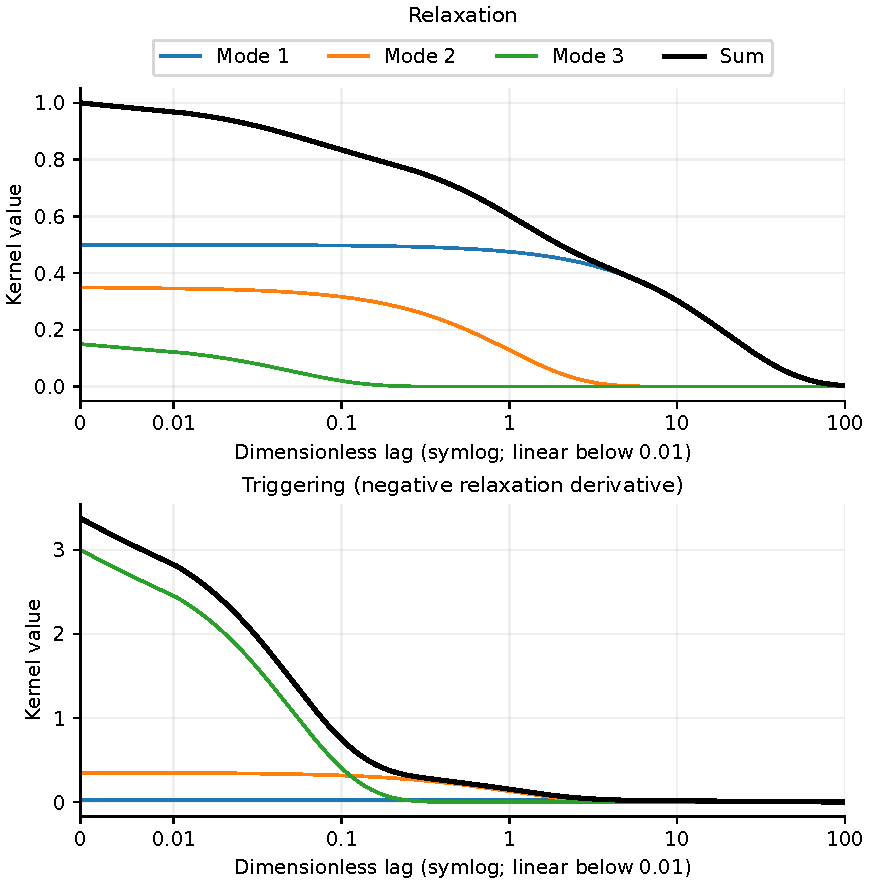
\includegraphics[width=0.95\linewidth]{finite_memory.pdf}
\caption{A dimensionless toy finite mixture with weights $(0.5,0.35,0.15)$ and rates $(0.05,1,20)$. The relaxation $\Phi$ and its negative derivative $h$ weight the same modes differently. Curves are direct evaluations of the displayed finite sums; they are not fits, simulations or an exact Mittag--Leffler kernel.}
\label{fig:finite_memory}
\end{figure}

In the physical model \(w_j\) is dimensionless, \(\vartheta_j\) and \(h\) have inverse-time units, \(\Phi\) is dimensionless, \(\rho\) is stress per unit time, and \(g(M)\) is measured in stress units. The jump \(\vartheta_j\kappa(M)\) has the units of \(U_j\). With no history, the sums in \eqref{eq:finite-X-mild}--\eqref{eq:finite-H-mild} are empty.

\section{The diagnostic model and observation}\label{sec:model_diagnostic}

For diagnostic work, retain a stress relaxation kernel \(\Phi_s\) and a normalized triggering density \(h_e\), initially allowing them to vary separately. Let \((T_i,Q_i)\) denote the accepted event times and their marks. Define the strictly prior cumulative release and excitation sums by
\begin{equation}\label{eq:diagnostic-sums}
G_s(t)=\sum_{0<T_i<t}g(Q_i)\Phi_s(t-T_i),
\qquad
H_e(t)=\sum_{0<T_i<t}\kappa(Q_i)h_e(t-T_i),
\end{equation}
and adopt the diagnostic intensity
\begin{equation}\label{eq:diagnostic-intensity}
\lambda_\eta(t)=B(t)\exp\{-\eta G_s(t)\}+nH_e(t).
\end{equation}

\begin{figure}[htb]
\centering
\includegraphics[width=0.95\linewidth]{model_architecture.pdf}
\caption{Physical loading and the independent-background diagnostic answer different questions. The left panel illustrates empty prehistory and equal initial stress coordinates $Z_j(0)=X_0$; arbitrary finite initial coordinates require the mode sum in \eqref{eq:finite-X-mild}. The physical model feeds loading through stress; the diagnostic specifies a background and suppresses its contribution by accumulated release. Triggering remains additive. The unit-productivity convention, with $n$ outside $H_e$, applies to the diagnostic.}
\label{fig:model_architecture}
\end{figure}
The baseline \(B(t)\) is deterministic at fixed parameters and specified independently of the stress-kernel family. A useful choice is \(B(t)=A\exp\{d x_{\mathrm{trend}}(t)\}\), where \(A=e^a>0\) and \(x_{\mathrm{trend}}(t)=2t/T_0-1\) for a declared fixed clock scale \(T_0>0\) (take \(T_0=T\) for the normalized single-window formulation). It is not generated by stress loading or by the marks. The strict inequalities in \eqref{eq:diagnostic-sums} are deliberate: an event is accepted before its mark is drawn, so its own release and productivity cannot enter its intensity.

This section adopts a convention change once and for all: diagnostic productivity is scaled to have unit mean,
\[
\E _F\kappa(Q)=1,
\]
while the coefficient \(n\) is retained \emph{outside} \(H_e\) in \eqref{eq:diagnostic-intensity}. In the physical model, by contrast, \(n=\E _F\kappa(M)<1\) is the mean carried by the productivity marks themselves. The diagnostic normalisation removes that mean from the marks and displays it explicitly as a coefficient. This is a bookkeeping convention, not an assertion that realised productivity is one, and it is not used to reinterpret the autonomous physical stability theorem.

The physical exponential link \eqref{eq:physical-link} embeds loading through \(X\): a constant \(\rho\) shifts the physical stress state and therefore changes \(\Psi(X)\). The time-dependent baseline \(B(t)\) in \eqref{eq:diagnostic-intensity} is an independently specified background. It does not replace \(\Psi(X)\) in the autonomous invariant-law theorem; that theorem does not cover externally varying \(B(t)\).

The shared subfamily imposes the identity \(h_e=-\Phi_s'\). This has substantive model content: the instantaneous excitation density is the negative derivative of the same kernel that governs stress relaxation. Consequently the decay of past stress and the contribution of a mark to the future compensator come from one memory structure, including its normalisation. Choices of \(\Phi_s\) and \(h_e\) that do not satisfy this identity define a separate-memory model. Normalization alone does not impose their equality.

A ground process records only the event times \(T_i\), whereas a marked process records the pairs \((T_i,Q_i)\). The ground law is a projection of the marked law. The event-time contribution to a joint marked likelihood, evaluated using observed past marks, is a different object from the marginal likelihood of times alone. Event times alone generally do not identify \(g\) and \(\kappa\) separately, nor their within-mark dependence, without an additional mark model. Conversely, the marked likelihood includes both ground acceptance probabilities and mark densities. Since marks are fresh after acceptance, past marks enter \eqref{eq:diagnostic-intensity} through the strict sums \eqref{eq:diagnostic-sums}, while a newly drawn mark first affects the future. This observational distinction is essential: marginalizing to times alone and evaluating a joint marked likelihood answer different questions.



The likelihoods studied below condition on a declared starting history. Empty prehistory is a model assumption rather than a statement that no earlier earthquakes occurred. Likewise, a fresh common mark law does not establish completeness or homogeneous measurement of the observed catalogue. Unobserved parents, omitted regions and uncertain magnitudes can change the relationship between the mathematical history and its recorded counterpart. The subsequent identification statements concern the declared complete marked process; their transfer to an earthquake catalogue requires an observation model.


\section{Master model and parameter dictionary}\label{sec:master-models}

The same letter can occur in a mathematical proof and in an archived program field. The following dictionary fixes the scientific meaning across the empirical chapters; explicitly local theoretical uses retain their stated assumptions. In particular, $X_{\rm phys}$ denotes latent physical stress when a distinction is needed, whereas $x_{\mathrm{trend}}(t)=2t/T_0-1$ is an affine clock, not a stress measurement. The earlier physical equations use $X$ for the former. A likelihood is written $\ell_{\rm score}$ when it could be confused with the LI range $\ell$; the auxiliary frozen response slope is a separate local theoretical quantity.

\begin{longtable}{@{}p{.17\textwidth}p{.77\textwidth}@{}}
\caption{Unified parameter meanings. Bounds and estimated/supplied status are procedure-specific and remain in the experimental chapters.}\label{tab:parameter-dictionary}\\
\toprule Symbol & Meaning \\\midrule\endfirsthead
\toprule Symbol & Meaning \\\midrule\endhead
$a,d$ & Log immigrant/background amplitude and affine-clock trend. Physical exponential-link slope $b$ is a different parameter. \\
$\widetilde a,\widetilde d$ & Exposure-orthogonalized background coordinates; a feasible reparameterization need not alter the represented intensity. \\
$n$ & Diagnostic excitation amplitude with unit-mean productivity; in the autonomous physical theorem it instead denotes the mean of the productivity mark. \\
$\eta$ & Nonnegative attenuation strength of the stated diagnostic history feature. \\
$\alpha,\tau$ & Mittag--Leffler fractional order and temporal scale; the implemented finite mixture is explicitly distinguished from the exact kernel. \\
$c,p$ & Omori time offset and power, with normalized density $k_O$ below. The magnitude-class cut is a separately declared threshold, not this time offset. \\
$r,\beta$ & Productivity exponent and exponential magnitude-excess rate. A training-only rate estimate and a freely fitted productivity exponent are different nuisance decisions. \\
$\omega$ & Redistribution share in the discrete spatial routing continuation. \\
$\sigma$ & Excitation spatial scale in the declared projected-domain density; a fitted/grid-selected model scale is not a measured interaction distance. \\
$\ell,\psi$ & LI attenuation range in kilometres and memory in days. Both disappear from the law at exact $\eta=0$. \\
$h,\delta$ & Magnitude-class association and parent-class fertility contrast. These do not denote the triggering density $h_e$ or a score difference $\Delta$. \\
\bottomrule
\end{longtable}

\begin{table}[htbp]\centering\small
\caption{Procedure names used in Parts III--IV. Names identify archived fitted recipes rather than new universal model families.}\label{tab:arm-dictionary}
\begin{tabularx}{\textwidth}{@{}lXX@{}}
\toprule Arm & Temporal law & Spatial/benchmark role \\\midrule
FC & Fixed-scale ML & Continuous reference-weighted offspring density \\
FL & Fixed-scale ML & Cell-lift offspring counterpart \\
MC & Free common-scale ML & Continuous offspring density \\
OC & Omori & Continuous reference-weighted offspring density \\
OL & Omori & Cell-lift offspring counterpart \\
EP & Omori ETAS adaptation & Separately fitted unweighted inverse-power radial offspring law \\
N0 & No offspring excitation & Separately refitted smooth immigrant background \\
LI & Matched OC excitation & Unrenormalized immigrant-only local attenuation \\
\bottomrule\end{tabularx}\end{table}

The labels FC through OL refer to the final smooth-background comparisons unless a factorial background is explicitly named. The earlier factorial also crosses cell and KDE-enriched backgrounds. EP is an excitation model; it is neither the no-trigger N0 recipe nor a constant-Poisson optimization floor. Comparisons of whole procedures must not be described as single-parameter inhibition ablations.

\section{Marked history and spatial observation laws}

For a magnitude excess $q$ under the working exponential law, the normalized productivity is
\[
 \kappa_r(q)=(1-r)e^{\beta rq},\qquad 0\leq r<1.
\]
Its unit mean is a property of that working law. The free-productivity experiment estimates $r$ within its declared continuous box; it is not a grid permitting $r\geq1$. The class-history extension replaces the fresh marginal mark allocation by a predictable class probability and a conditional within-class density. Its mark score includes that class probability once. Chapter~\ref{ch:temporal-extensions} gives the Perron normalization and explains why association can affect a joint fit without directly altering a fixed-history ground intensity after effective-scale matching.

On a fixed projected domain $D$, a noninhibited continuous model has
\begin{align}
 \lambda(t,z)&=e^{a+dx_{\mathrm{trend}}(t)}b_{\rm bg}(z)+nH(t,z),\label{eq:unified-spatial-law}\\
 H(t,z)&=\sum_{t_j<t}\kappa_j k_\theta(t-t_j)s_\sigma(z\mid z_j),\nonumber\\
 k_O(u)&=(p-1)c^{p-1}(u+c)^{-p},\qquad u>0,\quad c>0,\quad p>1,\nonumber\\
 s_\sigma(z\mid z_j)&=\frac{b_{\rm ref}(z)(1+\|z-z_j\|^2/\sigma^2)^{-2}}{\int_D b_{\rm ref}(v)(1+\|v-z_j\|^2/\sigma^2)^{-2}\,\dif v}.\label{eq:unified-OC-density}
\end{align}
Both spatial densities integrate to one over $D$; the temporal density integrates to one over all positive lags. Exposure uses the actual finite time window. The cell-lift counterpart allocates target-cell mass using its declared centre-based rule and spreads that mass uniformly inside the cell, retaining actual parent coordinates. EP normalizes a separately fitted radial law directly against projected area without $b_{\rm ref}$. Thus a location contrast always specifies its measure and reference.

Continuous local inhibition changes only the immigrant contribution:
\begin{align}
 \lambda_{\rm LI}(t,z)&=e^{a+dx_{\mathrm{trend}}(t)}b_{\rm bg}(z)e^{-\eta G(t,z)}+nH_{\rm OC}(t,z),\label{eq:unified-LI}\\
 G(t,z)&=\sum_{t_j<t}e^{-(t-t_j)/\psi}(1+\|z-z_j\|^2/\ell^2)^{-2}.\nonumber
\end{align}
The stress multiplier is one for every eligible recorded parent. The attenuation field is not a normalized spatial density; renormalizing the attenuated immigrant term would change the model. The observed California and synthetic-control clocks have distinct declared $T_0$, given in Chapter~\ref{ch:local-inhibition}. Exact $\eta=0$ restores OC at matching shared coordinates and makes every $\ell,\psi$ pair observationally equivalent. This boundary is the spatial counterpart of the identifiability limitation in Chapter~\ref{ch:identifiability}.

\section{Canonical proper-score semantics}\label{sec:master-scores}

Let $R(t)=\int_D\lambda(t,z)\,\dif z$ and let $\mathcal W$ be the scored window. All quantities below use the same fitted state and the same predictable observed history:
\begin{align}
 P&=\sum_{i\in\mathcal W}\log\lambda(t_i,z_i),&
 Q&=\sum_{i\in\mathcal W}\log R(t_i),\nonumber\\
 E&=\int_{\mathcal W}\int_D\lambda(t,z)\,\dif z\,\dif t,& C&=-E,\label{eq:master-PQECM}\\
 M&=\sum_{i\in\mathcal W}\log f(m_i\mid\mathcal H_{t_i},t_i,z_i).&&\nonumber
\end{align}
Thus
\begin{equation}\boxed{\begin{aligned}
 \text{Timing}&=Q+C=Q-E,\\
 \text{Conditional location}&=P-Q,\\
 \ell_{\rm score}&=P+C+M=\text{Timing}+\text{Conditional location}+M.
\end{aligned}}\label{eq:master-score-identity}\end{equation}
For temporal laws $P=Q$ and the conditional-location term is zero. For class-history laws the conditional class probability belongs to $M$, avoiding double counting. $E$ is nonnegative exposure, with expected-count dimension; it contributes negatively to a log score. A candidate-minus-reference difference obeys $\Delta C=-\Delta E$ and $\Delta\ell_{\rm score}=\Delta P+\Delta C+\Delta M$. Positive differences favour the candidate. There is no allocation of national exposure to event-only geographical groups unless an explicit spatial intensity supplies it.

\begin{table}[htbp]\centering\small
\caption{Master score-semantics crosswalk. Raw keys remain unchanged in the saved authorities; their scientific meaning is translated here.}\label{tab:score-crosswalk}
\fbox{\begin{minipage}{.94\textwidth}
\begin{tabularx}{\linewidth}{@{}XX@{}}
\toprule Saved context/key & Canonical meaning \\\midrule
Early temporal or LI pooled raw \texttt{E} & Event point-logsum contrast $\Delta P$ (temporal $\Delta Q$), not positive exposure \\
Early temporal or LI pooled raw \texttt{C} & Signed exposure contrast $\Delta C=-\Delta E$ \\
Sequence \texttt{timing\_compensator} & Difference $\Delta E$ in nonnegative exposure; it can have either sign and is subtracted \\
Benchmark \texttt{integrated\_intensity} & $E$ in arm rows, $\Delta E$ in contrast rows \\
JMA \texttt{positive\_C} / \texttt{signed\_negative\_C} & Positive exposure / its negative contribution \\
Marginal mark score & $M$, included once; it cancels only when the compared conditional mark laws agree \\
\bottomrule\end{tabularx}
\end{minipage}}
\end{table}
The pinned \path{validation/authorities/score_field_semantics_v2.json} is the documentary authority for this translation. It changes neither source fields nor scalar values. The repeated score check in Chapter~\ref{ch:design} fixes signs before any table is interpreted.

\chapter{Finite-Mode Stability and Exact-Memory Obstructions}\label{chap:stability}\label{ch:stability}

The finite-mode model admits a comparatively complete stability theory under autonomous loading and integrable marks. The theory combines a branching domination, a Lyapunov function, a synchronous coupling and a small-set estimate. Kernel approximation is then controlled on a fixed horizon. Finally, exact memory reveals a sharp obstruction without feedback and a resolvent response for an associated linear system; neither statement supplies a general nonlinear stationary theory.

\begin{figure}[htb]
\centering
\includegraphics[width=0.95\linewidth]{theory_scope.pdf}
\caption{The positive results have different assumption sets and limiting regimes. Finite-mode invariant laws, fixed-horizon approximation and the auxiliary response do not combine into a nonlinear exact-memory ergodicity theorem.}
\label{fig:theory_scope}
\end{figure}

\paragraph{Initialization and theorem scope.}
The autonomous finite-mode result concerns the stated finite-dimensional state
and its admissible initial states. It must be distinguished from the later
finite-horizon kernel comparison, which fixes a common finite initial stress
and no prehistory, and from the marked-resolvent identity, which assumes scalar
initial stress $X_0\Phi(t)$, zero initial excitation and no additional prehistory.
An arbitrary initialized excitation state contributes an additional homogeneous
term; it is not covered by silently reusing that scalar resolvent display.
None of these statements proves convergence of invariant laws as the number of
modes increases. The physical stress coordinate in this chapter is the
theoretical state, rather than the observed diagnostic's affine time coordinate.

\section{Autonomous finite-mode stability}\label{sec:finite-stability}

Fix the finite index set \(j\in\{1,\ldots,m\}\), \(m<\infty\), from Section~\ref{sec:model_physical}, and return to the physical convention \(n=\E _F\kappa(M)\). Suppose \(m_1<\infty\), \(n<1\), and \(\Psi:(-\infty,\bar x]\to(0,\infty)\) is nondecreasing and Lipschitz on the whole half-line. Write \(\bar\Psi=\Psi(\bar x)\). Put
\[
y_j=x_j^*-Z_j,\qquad Y=\sum_jw_jy_j,\qquad
W=\sum_j\frac{w_jU_j}{\vartheta_j},\qquad V=1+Y+cW,
\]
where
\begin{equation}\label{eq:c-choice}
c>\frac{m_1}{1-n}.
\end{equation}
The following theorem concerns constant \(\rho\) and fixed \(\Psi\); it is not a theorem about a time-varying diagnostic baseline.

\begin{theorem}[Finite-mode stability]\label{thm:finite_mode}
From every finite state in \(\mathcal X\), the autonomous finite-mode model has a pathwise unique, non-explosive, cadlag strong Markov construction and a Feller semigroup \(P_t\). There is a unique invariant probability \(\pi\) satisfying \(\pi(V)<\infty\). For suitable positive \(\epsilon,\beta,C,r\), with
\[
\|z-z'\|=\sum_jw_j\bigl(|Z_j-Z'_j|+|U_j-U'_j|\bigr),\qquad
d_\epsilon(z,z')=1\wedge\frac{\|z-z'\|}{\epsilon},
\]
and
\[
\widetilde d(z,z')=
\sqrt{d_\epsilon(z,z')\{1+\beta V(z)+\beta V(z')\}},
\]
one has
\begin{equation}\label{eq:weighted-contraction}
W_{\widetilde d}(P_t(z,\cdot),\pi)
\leq Ce^{-rt}\sqrt{1+V(z)},\qquad t\geq0.
\end{equation}
In particular, \(P_t(z,\cdot)\) converges weakly to \(\pi\).
\end{theorem}

Here \(W_c\) is the infimum of the expected cost \(c\) over couplings. The weighted cost \(\widetilde d\) need not satisfy a triangle inequality; the conclusion is not a total-variation mixing statement.

The constants generally depend on the rates, weights, \(m_1\), \(n\), the Lipschitz constant of \(\Psi\) and \(\bar\Psi\). No uniformity is claimed as \(\vartheta_{\min}=\min_j\vartheta_j\) tends to zero; the contractive time and the selected radius may deteriorate in that limit.

\begin{proof}
\emph{Construction and nonexplosion.} Use a marked Poisson embedding with thinning by the predictable intensity \(\Psi(X)+H\). The process is dominated by a marked Hawkes process with immigration \(\bar\Psi\), kernel
\[
h_d(t)=\sum_jw_j\vartheta_je^{-\vartheta_jt},
\]
and initial excitation \(\sum_jw_jU_j(0)e^{-\vartheta_jt}\). The latter integrates to \(W(z)\), and each cluster has expected total size \(1/(1-n)\). For every nonnegative mark weight \(\chi\) with finite mean,
\begin{equation}\label{eq:cluster-moment}
\E _z\sum_{T_i\leq T}\chi(M_i)
\leq\frac{\E _F\chi(M)}{1-n}
\{\bar\Psi T+W(z)\}.
\end{equation}
A generation is created before its marks are drawn, so \eqref{eq:cluster-moment} remains valid when \(\chi\) and \(\kappa\) are correlated. Finite expected counts imply nonexplosion; the deterministic flow and fresh Poisson increments yield the strong Markov property.

\emph{Lyapunov estimate.} Since the flow gives \(\dot Y=-\sum_jw_j\vartheta_jy_j\) and \(\dot W=-H\), while a jump adds \((g,\kappa)\), the extended generator satisfies
\[
\mathcal AV
=-\sum_jw_j\vartheta_jy_j-\delta H+(m_1+cn)\Psi(X),
\qquad
\delta=c(1-n)-m_1>0.
\]
Because \(\Psi(X)\leq\bar\Psi\) on \(\mathcal X\), direct comparison with the positive relaxation terms gives
\begin{equation}\label{eq:generator-bound}
\mathcal AV\leq-\kappa_V V+D,
\end{equation}
where
\[
K_0=(m_1+cn)\bar\Psi,\qquad
\kappa_V=\vartheta_{\min}\min\{1,\delta/c\},\qquad
D=\kappa_V+K_0.
\]
The weighted jump bound \eqref{eq:cluster-moment} makes the stopped compensated jump integral integrable. Applying the product formula to \(e^{\kappa_V t}V(z_t)\) and then Fatou's lemma gives
\begin{equation}\label{eq:lyap-moment}
P_tV(z)\leq e^{-\kappa_V t}V(z)+\frac{D}{\kappa_V}(1-e^{-\kappa_V t}).
\end{equation}

\emph{Coupling and smallness.} Couple two copies synchronously until their first unmatched event \(\sigma\). Identical jumps cancel before \(\sigma\), so
\[
\|z_t-z'_t\|\leq e^{-\vartheta_{\min}t}\|z-z'\|
\]
on \(\{\sigma>t\}\). Bounding the compensator of the difference of their rates by \(L\|z_t-z'_t\|\), with \(L=\max\{L_\Psi,1\}\), gives
\[
\mathbb P(\sigma\leq t)\leq
\frac{L}{\vartheta_{\min}}\|z-z'\|.
\]
Thus, whenever \(d_\epsilon(z,z')<1\),
\begin{equation}\label{eq:coupling-contraction}
W_{d_\epsilon}(P_tz,P_tz')
\leq\left(e^{-\vartheta_{\min}t}
+\frac{L\epsilon}{\vartheta_{\min}}\right)d_\epsilon(z,z').
\end{equation}
First fix \(R=4D/\kappa_V\) from the Lyapunov bound. Because the mode set is finite, \(\{V\leq R\}\) is compact and has finite diameter \(D_R\). Next choose \(\epsilon>0\) so that \(L\epsilon/\vartheta_{\min}\leq1/4\), and then choose \(t_0\) so that
\[
e^{-\vartheta_{\min}t_0}\leq1/4,
\qquad e^{-\vartheta_{\min}t_0}D_R\leq\epsilon/2.
\]
Thus \eqref{eq:coupling-contraction} has coefficient at most \(1/2\) for every \(t\geq t_0\). On the fixed sublevel set, event-free flow decreases both \(Y\) and \(W\), and the event rate is at most \(\Lambda_R=\bar\Psi+\vartheta_{\max}R/c\).
Use the same marked Poisson random measure $\Pi$ for both
copies, with intensity $\dif s\,\dif u\,F(\dif m)$ and the
usual acceptance threshold. The event
\[
 \Pi\bigl([0,t]\times[0,\Lambda_R]\times\mathsf M\bigr)=0
\]
has probability $e^{-\Lambda_Rt}$, since $F$ has total mass one. On this
event both copies follow their event-free flows and their rates remain at
most $\Lambda_R$, so neither jumps. Thus the synchronous coupling gives probability at least $e^{-\Lambda_Rt}$ that neither copy jumps. Once \(e^{-\vartheta_{\min}t}D_R\leq\epsilon/2\),
\[
\sup_{V(z),V(z')\leq R}W_{d_\epsilon}(P_tz,P_tz')
\leq1-\tfrac12e^{-\Lambda_Rt}<1.
\]
The same coupling shows that the state at a fixed time converges in probability as the initial state varies continuously. Expectations of bounded continuous functions therefore converge, establishing the Feller property. Taking \(t=t_0\) verifies contraction and smallness at the same time; the choices were made in the order \(R,\epsilon,t_0\).

Together with \eqref{eq:lyap-moment} this verifies the Lyapunov, contraction and smallness hypotheses of \citet{HairerMattinglyScheutzow2011}, Theorem~4.8 in the author-final version. Their Corollary~4.11 adds existence under the Feller and completeness conditions used here. Existence also follows from tight time-averaged laws, compact sublevels and \eqref{eq:lyap-moment}. The contraction time provided by the theorem may be later than the time used to check the hypotheses. Replacing \(d_\epsilon\) by \(\widetilde d\) and iterating the resulting contraction, while using \eqref{eq:lyap-moment} for the residual time, gives \eqref{eq:weighted-contraction}. No second mark moment is required.

To see that every invariant probability has the same finite moment without subtracting potentially infinite integrals, suppose \(PV\leq aV+b\) with \(a<1\), and put \(f_K(v)=\min(v,K)\). If \(\nu\) is invariant, concavity gives
\[
\nu\{f_K(V)-f_K(aV+b)\}\leq0.
\]
For \(K\geq b/(1-a)\), the integrand is at least
\([(1-a)V-b]\mathbf 1_{\{V\leq K\}}\). Hence
\(\nu(V\mathbf 1_{\{V\leq K\}})\leq b/(1-a)\). Monotone convergence and \eqref{eq:lyap-moment} yield \(\nu(V)\leq D/\kappa_V\). The weak Harris theorem supplies uniqueness.
\end{proof}

Under the invariant law, let \(\Lambda=\pi(\Psi(X)+H)>0\). Since \(\pi(V)<\infty\), every \(U_j\) and \(|Z_j|\) is integrable, and \(\Lambda<\infty\). The mild coordinate equations and fresh-mark compensation therefore give, for \(t>0\),
\[
\begin{aligned}
\pi(U_j)&=e^{-\vartheta_jt}\pi(U_j)
             +n\Lambda(1-e^{-\vartheta_jt}),\\
\pi(Z_j)&=e^{-\vartheta_jt}\pi(Z_j)
             +\frac{\rho-m_1\Lambda}{\vartheta_j}
               (1-e^{-\vartheta_jt}).
\end{aligned}
\]
All expectations are finite before cancellation: the expected marked jump sums are bounded by their first mark moments times \(\Lambda t\). Cancelling \(1-e^{-\vartheta_jt}>0\), then using \(H=\sum_jw_jU_j\), gives
\[
\pi(U_j)=n\Lambda,\qquad
\pi(Z_j)=\frac{\rho-m_1\Lambda}{\vartheta_j},\qquad
\Lambda=\frac{\pi(\Psi(X))}{1-n},
\]
and hence
\[
\pi(X)=(\rho-m_1\Lambda)\sum_j\frac{w_j}{\vartheta_j}.
\]
Under \(\mathbb P_\pi\), intensity ergodicity and the compensated counting martingale give \(N(t)/t\to\Lambda\), while the fresh-mark strong law gives \(t^{-1}\sum_{T_i\leq t}g(M_i)\to m_1\Lambda\).

\begin{proposition}[Infinite stationary second moments]\label{prop:heavy-moments}
If \(\E _Fg(M)^2=\infty\), then \(\pi(Y^2)=\infty\) and consequently \(\pi(X^2)=\infty\). If \(\E _F\kappa(M)^2=\infty\), then \(\pi(W^2)=\infty\) and consequently \(\pi(H^2)=\infty\).
\end{proposition}

\begin{proof}
Let \(\Phi_d(t)=\sum_jw_je^{-\vartheta_jt}>0\). The mild equations for the nonnegative depletion modes \(y_j\) and the integrated excitation modes give, on any stationary interval of length \(t\),
\[
Y(0)^2\geq\Phi_d(t)^2\sum_{-t<T_i\leq0}g(M_i)^2,
\qquad
W(0)^2\geq\Phi_d(t)^2\sum_{-t<T_i\leq0}\kappa(M_i)^2.
\]
Replace a squared mark by \(g_K^2=(g\wedge K)^2\). Fresh-mark compensation, applied before each mark is revealed, gives
\[
\E _\pi\sum_{-t<T_i\leq0}g_K(M_i)^2
=\E _Fg_K(M)^2\int_{-t}^0\E _\pi\lambda_s\,\dif s
=t\Lambda\E _Fg_K(M)^2.
\]
Thus
\(\pi(Y^2)\geq\Phi_d(t)^2t\Lambda\E _Fg_K(M)^2\).
Letting \(K\uparrow\infty\) proves the first implication. The productivity argument is identical. Since \(X=\bar x-Y\), infinite \(\pi(Y^2)\) implies infinite \(\pi(X^2)\). Since \(W\) and \(H\) are comparable through the finitely many positive rates, infinite \(\pi(W^2)\) implies infinite \(\pi(H^2)\).
\end{proof}

The argument concerns the corresponding jump transform: it asserts stress divergence when the stress-mark second moment diverges, and excitation divergence when the productivity second moment diverges. Finite first-moment stability and infinite stationary variance coexist. A quadratic theorem under stronger finite-moment assumptions is not contradicted; those stronger assumptions cannot be inferred for an untruncated heavy-tailed fitted law.

\section{Fixed-horizon kernel approximation}

Let \(\Phi\) and \(\Phi_d\) be nonnegative decreasing absolutely continuous kernels, normalised to one at zero and tending to zero at infinity, so that \(h=-\Phi'\) and \(h_d=-\Phi_d'\) are probability densities. Use the same scalar initial term \(X_0\Phi(t)\) (and \(X_0\Phi_d(t)\)), zero initial excitation, constant loading, no prehistory, fresh marks, and the first-moment assumptions above. In a finite mixture this scalar initial term means equal initial stress coordinates. These are not stationary initializations drawn from \(\pi_d\). Let \(\Psi\) be positive, nondecreasing and locally Lipschitz on \(\mathbb R\). For fixed \(T<\infty\), put
\[
B=A_T=|X_0|+\rho T,\qquad
K_T=\frac{\Psi(B)T}{1-n},
\]
\[
\Delta_\Phi=\sup_{[0,T]}|\Phi_d-\Phi|,
\qquad
\Delta_h=\int_0^T|h_d-h|.
\]

\begin{proposition}[Quantitative half-line approximation]\label{prop:quantitative-kernel}
If \(\Psi\) is Lipschitz on \((-\infty,B]\) with constant \(L_B\), then, under the same Poisson-measure coupling,
\begin{equation}\label{eq:quantitative-kernel}
\mathbb P(\text{marked catalogues differ on }[0,T])
\leq\min\{1,\;L_BT(A_T+m_1K_T)\Delta_\Phi+nK_T\Delta_h\}.
\end{equation}
For \(\Psi(x)=e^{a+bx}\), \(b\geq0\), one may take \(L_B=be^{a+bB}\).
\end{proposition}

\begin{proof}
All stresses remain at most \(B\). Until the two coupled processes first separate,
\[
|X_d(s)-X(s)|
\leq\Delta_\Phi\left(A_T+\sum_{T_i<s}g(M_i)\right),
\]
and the integrated excitation discrepancy is bounded by
\(\Delta_h\sum_{T_i\leq T}\kappa(M_i)\). Common pre-separation events form a subset of the reference events, which are dominated by the Hawkes process with immigration \(\Psi(B)\). Its expected event count is at most \(K_T\), while the corresponding weighted expectations are at most \(m_1K_T\) and \(nK_T\). Bounding the compensated difference of the two event intensities by the stress discrepancy and the excitation discrepancy and integrating its expectation gives \eqref{eq:quantitative-kernel}.
\end{proof}

Local Lipschitz continuity does not support the same linear error bound. It nevertheless gives qualitative convergence through a separate truncation.

\begin{proposition}[Qualitative local approximation]\label{prop:qualitative-kernel}
For \(R>0\), let \(L_R\) be a Lipschitz constant of \(\Psi\) on \([-|X_0|-R,B]\). Then
\begin{equation}\label{eq:qualitative-kernel}
\mathbb P(\text{catalogues differ on }[0,T])
\leq\min\left\{1,\frac{m_1K_T}{R}
+L_RT(A_T+R)\Delta_\Phi+nK_T\Delta_h\right\}.
\end{equation}
\end{proposition}

\begin{proof}
On common prehistories whose cumulative release is at most \(R\), both stresses lie in the compact interval on which \(L_R\) is valid, and the half-line calculation applies with \(R\) in place of the full released mass. The complement has probability at most \(m_1K_T/R\) by Markov's inequality. Fix \(R\), let the two kernel errors tend to zero, and then let \(R\to\infty\).
\end{proof}

Thus half-line Lipschitz continuity gives a quantitative error rate, whereas local Lipschitz continuity gives only qualitative fixed-horizon convergence. A finite half-line constant cannot be inferred from local Lipschitz continuity. The constants depend on \(T\) through \(B\), \(K_T\) and the relevant Lipschitz constant, and can deteriorate rapidly as the horizon increases. Neither bound is uniform in \(T\), and neither exchanges the kernel-approximation and long-time limits.

\section{Exact-memory obstruction and response}

Exact memory neither prevents all stationary constructions nor yields a general nonlinear stationary theorem. The first point is visible already in a zero-history model without feedback.

\begin{proposition}[No-feedback obstruction]\label{prop:exact-obstruction}
Let \(0<\alpha<1\), \(\tau>0\), and
\(\Phi(t)=E_\alpha(-(t/\tau)^\alpha)\). Consider the zero-history model with \(X_0=0\), constant immigration rate \(\mu>0\), no triggering, and loading \(\rho=\mu\E  S\). Let \(N(\dif v,\dif S)\) be Poisson with intensity \(\mu\,\dif v\,F_S(\dif S)\), let \(\widetilde N\) be its compensated measure, and define
\[
X(t)=-\int_0^t\Phi(t-v)S\,\widetilde N(\dif v,\dif S).
\]
If \(S=1\), no sequence \(t_k\to\infty\) has a tight subsequence of stress laws for \(\alpha\leq1/2\). If \(P(S>s)=s^{-q}\) for \(s\geq1\) and \(1<q<2\), the corresponding obstruction occurs when \(\alpha q\leq1\). For \(S=1\), \(\alpha>1/2\) admits a stationary two-sided compensated moving average in \(L^2\), and the zero-history one-time laws converge. For Pareto marks, \(\alpha q>1\) admits such a construction in \(L^p\) for every \(1/\alpha<p<q\).
\end{proposition}

\begin{proof}
The finite-interval Poisson exponential formula gives
\begin{equation}\label{eq:obstruction-cf}
\left|\E  e^{iuX(t)}\right|
=\exp\left\{-\mu\int_0^t
\E _F\{1-\cos(uS\Phi(v))\}\,\dif v\right\}.
\end{equation}
For unit marks, the integrand is asymptotic to \(u^2\Phi(v)^2/2\) for fixed \(u\neq0\). For Pareto marks and \(0<x\leq1\), restricting \(S\) to \([1/x,2/x]\) yields
\[
\E _F\{1-\cos(xS)\}
\geq(1-\cos1)(1-2^{-q})x^q.
\]
Since
\(\Phi(v)\sim\tau^\alpha v^{-\alpha}/\Gamma(1-\alpha)\),
the modulus \eqref{eq:obstruction-cf} tends to zero at every nonzero frequency in the stated regimes. Tightness would give a weak subsequential limit; by the continuity theorem its characteristic function would be continuous at zero, but the limit would equal zero at every \(u\neq0\) and one at \(u=0\), a contradiction.

Above the threshold, the two-sided compensated integrals converge in \(L^2\) by the isometry for unit marks. For Pareto marks, choose \(1/\alpha<p<q\). Then \(\E  S^p<\infty\) and \(\int_0^\infty\Phi(v)^p\,\dif v<\infty\), so the compensated Poisson \(L^p\) estimate gives the two-sided construction.
\end{proof}

This is a no-feedback statement. It does not assert nonstationarity of the stress-sensitive nonlinear model, and a stationary compensated construction is not the subtraction of two separately divergent, uncompensated past integrals.

Even the stationary unit-mark construction for \(\alpha>1/2\) has unbounded upper support. At a fixed stationary time split its stress as
\[
X_\infty=-\int_0^L\Phi(u)\,\widetilde N(\dif u)+R_L,
\qquad \E R_L^2=\mu\int_L^\infty\Phi(u)^2\,\dif u\longrightarrow0,
\]
where the recent and remote Poisson restrictions are independent. For any \(K\), choose \(L\) large enough that \(\mu\int_0^L\Phi(u)\,\dif u>K+1\) and \(\E R_L^2<1\). No recent event has probability \(e^{-\mu L}>0\), and \(\Pr(R_L>-1)>0\) by the second-moment bound. Their intersection gives \(X_\infty>K\). Hence \(\operatorname{ess\,sup}X_\infty=\infty\): finite variance does not provide a deterministic upper stress cap. For \(b>0\), \(e^{a+bX_\infty}\) is unbounded above, so the finite-mode half-line argument cannot be transferred to this law. Introducing that stress-dependent rate changes the no-feedback process and requires separate analysis; unbounded support alone proves neither nonexistence of a nonlinear invariant law nor divergence of the mean exponential rate.

For an auxiliary excitation-inclusive system, a positive stress-to-rate slope changes the response through an integrable resolvent with a heavy tail. Let \(m_1>0\), \(0\leq n<1\) and \(\ell>0\), and consider
\begin{equation}\label{eq:aux-response-equations}
x=-m_1\Phi*y,\qquad
y=\ell x+nh*y+\xi,\qquad
h=-\Phi',
\end{equation}
with zero initial perturbation and additive event-flux forcing \(\xi\). Set
\[
\gamma=m_1\ell,\qquad \beta_{\mathrm{rel}}=1-\alpha,\qquad
a_{\mathrm{rel}}=(1-n)\tau^{-\alpha}.
\]

\begin{proposition}[Excitation-inclusive response]\label{prop:auxiliary-response}
The causal solution of \eqref{eq:aux-response-equations} is
\(x=-m_1R_\gamma*\xi\), where
\begin{equation}\label{eq:response-transform}
\widehat R_\gamma(s)=\frac{1}{s+a_{\mathrm{rel}} s^{\beta_{\mathrm{rel}}}+\gamma}.
\end{equation}
For \(\gamma>0\), \(R_\gamma\) is completely monotone, \(R_\gamma(0+)=1\), \(\int_0^\infty R_\gamma(t)\,\dif t=1/\gamma\), and
\begin{equation}\label{eq:response-tail}
R_\gamma(t)\sim
\frac{a_{\mathrm{rel}}\beta_{\mathrm{rel}}}{\gamma^2\Gamma(1-\beta_{\mathrm{rel}})}t^{-1-\beta_{\mathrm{rel}}}.
\end{equation}
In particular, \(\int_0^\infty tR_\gamma(t)\,\dif t=\infty\).
\end{proposition}

\begin{proof}
Eliminating \(y\) in the Laplace domain gives
\[
\widehat\Phi(s)=\frac{s^{\alpha-1}}{s^\alpha+\tau^{-\alpha}},
\qquad
\widehat h(s)=\frac{\tau^{-\alpha}}{s^\alpha+\tau^{-\alpha}}.
\]
Substitution into \eqref{eq:aux-response-equations} yields
\[
\widehat x(s)=-\frac{m_1s^{\alpha-1}\widehat\xi(s)}
{s^\alpha+\gamma s^{\alpha-1}+(1-n)\tau^{-\alpha}}
=-m_1\widehat R_\gamma(s)\widehat\xi(s),
\]
which is \eqref{eq:response-transform}. The reciprocal of the nonnegative complete Bernstein function \(s+a_{\mathrm{rel}} s^{\beta_{\mathrm{rel}}}+\gamma\) is a Stieltjes function, hence \(R_\gamma\) is completely monotone
\citep[Section~2.1]{MeerschaertToaldo2019}. Its spectral density is
\[
k_\gamma(r)=
\frac{a_{\mathrm{rel}}\sin(\pi\beta_{\mathrm{rel}})r^{\beta_{\mathrm{rel}}}}
{\pi\{[\gamma-r+a_{\mathrm{rel}} r^{\beta_{\mathrm{rel}}}\cos(\pi\beta_{\mathrm{rel}})]^2+
a_{\mathrm{rel}}^2r^{2\beta_{\mathrm{rel}}}\sin^2(\pi\beta_{\mathrm{rel}})\}},
\]
so \(R_\gamma(t)=\int_0^\infty e^{-rt}k_\gamma(r)\,\dif r\). The limits of \eqref{eq:response-transform} at infinity and zero give \(R_\gamma(0+)=1\) and \(\int R_\gamma=1/\gamma\). Near \(r=0\),
\[
k_\gamma(r)\sim
\frac{a_{\mathrm{rel}}\sin(\pi\beta_{\mathrm{rel}})}{\pi\gamma^2}r^{\beta_{\mathrm{rel}}}.
\]
Rescaling the spectral integral and using the gamma reflection formula gives \eqref{eq:response-tail}. The tail exponent \(-1-\beta_{\mathrm{rel}}\) lies between \(-2\) and \(-1\), so the first temporal moment diverges.
\end{proof}

The weak-feedback crossover is equally explicit. Put \(t_\gamma=(a_{\mathrm{rel}}/\gamma)^{1/\beta_{\mathrm{rel}}}\). As \(\gamma\downarrow0\), the probability densities \(\gamma t_\gamma R_\gamma(t_\gamma u)\) on \((0,\infty)\) converge weakly to the law with Laplace transform \((1+z^{\beta_{\mathrm{rel}}})^{-1}\), because
\[
\int_0^\infty e^{-zu}\gamma t_\gamma R_\gamma(t_\gamma u)\,\dif u
=\frac{1}{1+z^{\beta_{\mathrm{rel}}}+z/(\gamma t_\gamma)}
\longrightarrow\frac{1}{1+z^{\beta_{\mathrm{rel}}}}.
\]
At \(\gamma=0\), \(R_0(t)=E_\alpha(-a_{\mathrm{rel}}t^\alpha)\) is not integrable. The crossover is separated from the early-time scale \(a_{\mathrm{rel}}^{-1/\alpha}\) only when \(\gamma\ll a_{\mathrm{rel}}^{1/\alpha}\). This is a statement about an auxiliary impulse response, not a nonlinear mixing time.

An abstract signed-response equation illustrates the limit of this resolvent method. Let \(\psi:\mathbb R\to\mathbb R\), \(\psi(0)=0\), and consider
\[
y=\psi(x)+nh*y+\xi,\qquad
\mathcal E(x)=m_1\psi(x)-\gamma x.
\]
If \(\mathcal E\) is globally Lipschitz with constant \(L<\gamma\), the map
\[
x=-R_\gamma*(m_1\xi+\mathcal E(x))
\]
has contraction constant at most \(L\|R_\gamma\|_1=L/\gamma<1\) on bounded causal functions, and
\(\|x\|_\infty\leq m_1\|\xi\|_\infty/(\gamma-L)\). This nonempty abstract class includes the signed linear response \(\psi(x)=\gamma x/m_1\). For jointly measurable stationary forcing on \(\mathbb R\) with an almost surely uniform deterministic bound, the analogous two-sided causal resolvent map has a stationary fixed point by shift-equivariant Picard iteration. This assertion concerns the integrable-resolvent equation, not absolute convergence of a two-sided \(\Phi*y\).

It is \emph{not} a global contraction criterion for the physical positive link. If \(\psi(x)=\Psi(x+x_*)-\Psi(x_*)\) on its lower-unbounded domain and \(\Psi>0\), then \(\psi(x)\geq-\Psi(x_*)\) and \(\mathcal E(0)=0\). For negative \(x\),
\[
\mathcal E(x)\geq\gamma|x|-m_1\Psi(x_*),
\]
so any global Lipschitz constant of \(\mathcal E\) is at least \(\gamma\). No differentiability assumption is needed for this obstruction. In particular, every positive nondecreasing physical link is excluded, not only the exponential example. A contraction restricted to a compact stress band would additionally require that the map preserve that band; no such invariant-band or exit control is proved here.

The obstruction and resolvent calculation therefore delimit the demonstrated scope. Neither supplies a generic stationary theorem for the nonlinear stress-sensitive exact-memory process.

\subsection{What the auxiliary response omits}

The actual marked process has two noise sources rather than a single prescribed event-flux input. In the physical productivity convention, define compensated marked measures by
\[
\dif M_g=\dif N_g-m_1\lambda\,\dif t,\qquad
\dif M_\kappa=\dif N_\kappa-n\lambda\,\dif t,
\]
where $N_g$ and $N_\kappa$ accumulate the corresponding marks. These martingales are generally correlated: both jump at the same events, and the two transforms of a fresh mark need not be independent. 

\begin{samepage}
In the following exact identity, \(\gamma>0\) is an auxiliary parameter added and subtracted algebraically; it is not an established lower physical restoring slope. Set $Q_\gamma=R_\gamma-nR_\gamma*h$, and let $X^+(t)$ denote post-event stress, including releases at time $t$. For scalar initial stress \(X_0\Phi(t)\), zero initial excitation and no additional prehistory, finite-horizon compensation and the same Laplace-resolvent algebra give the exact identity
\begin{align}
X^+(t)={}&X_0Q_\gamma(t)+\rho\int_0^tQ_\gamma(u)\,\dif u \notag\\
&+[R_\gamma*(\gamma X^+-m_1\Psi(X^+_-))](t) \notag\\
&-\int_{(0,t]}Q_\gamma(t-u)\,\dif M_g(u) \notag\\
&-m_1\int_{(0,t]}(R_\gamma*h)(t-u)\,\dif M_\kappa(u).
\label{eq:marked-resolvent}
\end{align}
\end{samepage}
Here $X^+_-(u)=X^+(u^-)$, and all assertions are on finite horizons under compensator integrability. At an event time, the intensity uses the left limit; the displayed post-event identity must be left-limited consistently if it is used to evaluate that intensity. The deterministic kernels in the two noise terms are bounded and integrable, but this does not by itself control the nonlinear residual in the second line. In particular, the stress can leave any band on which a positive lower slope is available. Establishing tightness or a uniform occupation bound outside that band remains a separate task. The identity explains the relevance of the auxiliary response while retaining the nonlinear term and both correlated mark martingales.

\paragraph{Compensation and cancellation.}
An event-free path has $\dif N_g=\dif N_\kappa=0$, but not
$\dif M_g=\dif M_\kappa=0$. Instead,
\[
  \dif M_g=-m_1\lambda\,\dif t,
  \qquad
  \dif M_\kappa=-n\lambda\,\dif t.
\]
The compensated integrals must therefore be retained even when no event
occurs. The causal kernels satisfy
\[
 Q_\gamma+nR_\gamma*h=R_\gamma,
 \qquad
 Q_\gamma+\gamma R_\gamma*\Phi=\Phi.
\]
For the stated initialization, put
$f=X_0\Phi+\rho(1*\Phi)$, where $(1*\Phi)(t)=\int_0^t\Phi(u)\,\dif u$.
In the following ordinary time convolutions write $X$ for $X^+$, retaining
$X_-$ in the predictable intensity. The original equations give
\[
 X=f-\Phi*\dif N_g,
 \qquad \lambda=\Psi(X_-)+h*\dif N_\kappa.
\]
Substitution of both compensated measures into the displayed identity,
followed by the first kernel relation, reduces its right-hand side to
\[
 X_0Q_\gamma+\rho(1*Q_\gamma)-Q_\gamma*\dif N_g
   +\gamma R_\gamma*X.
\]
The second kernel relation makes the first three terms
$X-\gamma R_\gamma*X$, proving the cancellation. These are finite-horizon
causal convolution identities under the stated integrability conditions;
no infinite-history transform of a nonlinear sample path or stationary
exact-memory limit is asserted.

The archival E04 worked example and expanded derivations remain in the public repository at \path{paper/supplements/explanatory_supplement.pdf}; compact standalone release bundles omit this supplement.

A uniform invariant-mean bound cannot be inferred from fixed-mode stability. If $\sup_d|\E _{\pi_d}X_d|<\infty$, $m_1>0$ and $A_d=\int_0^\infty\Phi_d(t)\dif t\to\infty$, stationary balance gives the following conditional implication; it establishes neither invariant-law convergence nor an exchange of limits:
\[
\E _{\pi_d}X_d=(\rho-m_1\Lambda_d)A_d
\quad\Longrightarrow\quad
m_1\Lambda_d\longrightarrow\rho.
\]



\chapter{Structural Identifiability, Boundary Singularity, and Regional Nonclosure}\label{chap:identifiability}\label{ch:identifiability}

An identifiability question asks whether distinct generative structures produce the same observed law. A visibility question asks how strongly those laws separate on a finite experiment. Exact nonidentification prevents recovery of the unidentified quantity from the observed law, whereas distinct laws can still be difficult to distinguish on a finite horizon. The distinction is essential here: stress memory disappears from the rate at zero feedback, yet under stronger assumptions it becomes identifiable when inhibition is active.

\section{Physical loading and the diagnostic family}

Let \(Q_i\) denote marks, let \(\Phi_s\) be a nonnegative normalized relaxation kernel, and put
\[
X(t)=X_0\Phi_s(t)+\rho\int_0^t\Phi_s(u)\,\dif u-G_s(t),
\qquad
G_s(t)=\sum_{T_i<t}g(Q_i)\Phi_s(t-T_i).
\]
The physical rate family is
\begin{equation}
\lambda_{\mathrm{phys}}(t)
=\exp\{a+bX(t)\}+nH_e(t),
\qquad
H_e(t)=\sum_{T_i<t}\kappa(Q_i)h_e(t-T_i).
\label{eq:physical-rate}
\end{equation}
Here \(\kappa\) is a unit trigger amplitude, \(\E \kappa(Q)=1\), and \(n\) is outside \(H_e\). Marks are generated from the common fresh-mark law specified for the experiment. The diagnostic experiment instead uses
\begin{equation}
\lambda_\eta(t)=B(t)e^{-\eta G_s(t)}+nH_e(t),
\qquad
B(t)=A e^{d x_{\mathrm{trend}}(t)},\qquad \eta\ge0,
\label{eq:diagnostic-rate}
\end{equation}
where \(A=e^a>0\) and \(x_{\mathrm{trend}}(t)=2t/T_0-1\) uses the fixed declared clock scale \(T_0>0\). This clock is distinct from physical stress \(X(t)\). The same event and mark parents supply \(G_s\) and \(H_e\). Thus \(nH_e\) has the same unit interpretation as in \eqref{eq:physical-rate}.

The independent background \(B(t)\) in the diagnostic family is not a reparameterization of the physical loading law. In the diagnostic model, \(B(t)=A e^{d x_{\mathrm{trend}}(t)}\) is an explicitly fitted background trajectory; in the physical model, the stress response is constrained by the relaxation kernel and by the latent initial stress. This distinction is part of the inferential target, not merely a matter of notation. It is also the reason a fitted background trend cannot by itself establish earthquake-induced inhibition. Productivity is displayed in the unit convention, with its branching coefficient separate.

\section{Exact nonidentification at zero feedback}

The first nonidentification result follows directly from the multiplicative role of \(b\). If the stress sensitivity \(b=0\) while \(X_0\) and \(\rho\) remain finite, then \(bX(t)=0\) for every history. Consequently the conditional intensity is
\[
\lambda(t)=\exp(a)+nH_e(t),
\]
which contains neither \(\Phi_s\) nor \(G_s\). Different relaxation kernels can therefore imply radically different latent stress trajectories while leaving the rate and the common mark law unchanged.

\begin{remark}[Stress-kernel nonidentification at zero feedback]
\label{prop:nonidentification}
Fix \(a\), \(n\), \(h_e\), the unit-mean transform \(\kappa\), and a common fresh-mark law. Two normalized relaxation kernels with the same finite \(X_0,\rho\) and \(b=0\) give identical observed marked laws, provided both constructions are nonexplosive. Indeed, their successive waiting-time hazards are both \(\exp(a)+nH_e\), and the accepted marks have the same conditional law. This constructs equal laws on each finite horizon; equality on nested windows extends to their generated infinite-horizon \(\sigma\)-field. The conclusion does not require a mark density.
\end{remark}

This observation uses equality of the fresh mark laws. Equality of ground intensities alone is not equality of marked laws if the conditional mark distributions differ: the same event times with different marks produce different full catalogue laws. The statement also concerns normalized relaxation kernels; it does not assert invariance to kernel-dependent changes in the trigger mechanism. The latent stress laws may be substantively different, including in their unobserved tails, even though every observed waiting time and mark has the same distribution.

In the diagnostic family the same argument applies at \(\eta=0\), holding background and triggering fixed. A shared-kernel restriction may still permit estimation of the kernel through triggering. Such estimation cannot validate the additional claim that an unobserved stress response has that same kernel.

There is a distinct singular closure as the positive stress sensitivity approaches zero. For \(b>0\), put \(p=bX_0\), \(q=b\rho\), and \(r=b\). The physical background component \(\mu_b=\exp(a+bX)\) satisfies
\[
\log\mu_b(t)=a+p\Phi_s(t)+q\int_0^t\Phi_s(u)\,\dif u-rG_s(t).
\]
Allowing \(r=0\) while \(q>0\) creates a deterministic kernel-shaped trend with no event-dependent inhibition. Reaching this closure requires \(\rho=q/r\) to diverge; retaining nonzero \(p\) also requires \(X_0=p/r\) to diverge. With fixed finite \(X_0\), therefore, \(p\to0\). The loading constraint \(\rho\ge0\) preserves \(q\ge0\). This trend-only closure and the finite-parameter \(b=0\) null are different hypotheses. A deterministic trend may identify aspects of \(\Phi_s\) through loading without identifying earthquake-induced inhibition or establishing \(h_e=-\Phi_s'\).

\section{Restricted active identification}

Nonidentification in the physical family does not mean that active inhibition is never identifiable. A deliberately restricted marked experiment can remove the zero-feedback ambiguity by exposing the nonlinear intervention term. The following statement is an idealized full-law result, not a finite-sample guarantee.

\begin{proposition}[Restricted active identification]
\label{prop:active_identification}
Consider the diagnostic family \eqref{eq:diagnostic-rate} with empty initial history, a positive continuous deterministic background \(B\), known positive continuous \(g\), and nonnegative \(\eta\). Let the known transform \(\kappa>0\) be continuous with \(\E \kappa(Q)=1\) and \(\kappa(q)\to\infty\), and let the common fresh mark law have a positive density on \([0,\infty)\). Let \(h_e\) be locally integrable at zero, continuous and positive for \(u>0\), normalized to integrate to one, and let \(\Phi_s\) be nonnegative continuous with \(\Phi_s(0)=1\). Assume all models are nonexplosive with finite mean event counts. Equality of two observed marked laws identifies \(B(t)\) on \([0,T]\), the product \(n h_e(u)\) for observed lags \(0<u<T\), and \(\eta\); if \(\eta>0\), \(\Phi_s\) is identical on \([0,T]\). For the scaled finite positive exponential-mixture family with known weights and relative rates, and \(n>0\), the mixture scale and \(n\) are also identified within that restricted family.
\end{proposition}

\begin{proof}
Before the first event \(G_s=H_e=0\), so the hazard is \(B(t)\). The distribution of the first waiting time identifies \(\int_0^tB(u)\,\dif u\), and continuity identifies \(B\) itself. Marked-law equality therefore permits comparison along a history containing one event at \(s\) with mark \(q\) and no further event before \(t\). Local integrability of \(h_e\) gives a positive no-further-event survival on each finite interval. For almost every \(s< t\) and \(q\ge0\), equality of the two hazards gives
\[
B(t)\exp\{-\eta g(q)\Phi_s(t-s)\}+n\kappa(q)h_e(t-s)
=
\widetilde B(t)\exp\{-\widetilde\eta g(q)\widetilde\Phi_s(t-s)\}
+\widetilde n\kappa(q)\widetilde h_e(t-s).
\]
Continuity extends this almost-everywhere identity to every finite \(q\) and positive observed lag. After \(B=\widetilde B\), divide by \(\kappa(q)\) and let \(q\to\infty\). The first term is bounded by \(B(t)\), while \(\kappa(q)\to\infty\); hence the normalized triggering term is identified as \(n h_e(u)=\widetilde n\widetilde h_e(u)\). Subtract this common term. The remaining background is positive on the observation window, so taking logarithms shows that \(\eta g(q)\Phi_s(u)=\widetilde\eta g(q)\widetilde\Phi_s(u)\). Dividing by the known positive \(g(q)\), and then letting \(u\downarrow0\) with \(\Phi_s(0)=1\), identifies \(\eta\). If \(\eta>0\), division by \(\eta\) identifies \(\Phi_s(u)\) throughout the observed window.

For the finite mixture \(h_e(u)=\sum_j w_j(c_j\tau_e)^{-1}\exp\{-u/(c_j\tau_e)\}\), with known positive \(c_j,w_j\) and unknown \(\tau_e>0\), the ratio \(-h_e'(0)/h_e(0)\) identifies the common scale \(\tau_e\) when the identified product \(n h_e\) is positive. Its value at zero then identifies \(n\).
\end{proof}

Several limitations are part of the result. If \(\eta=0\), the stress kernel is unidentified; if \(n=0\), the triggering scales are unidentified, even though the background may be known. The proof uses arbitrarily large marks across the full probability law. Bounded marks do not inherit this positive-identification proof: the limiting operation \(q\to\infty\) is unavailable, so a separate argument would be needed. Shared triggering may identify a trigger scale when \(\eta=0\), but it does not validate equality of the latent physical loading laws; the exact nonidentification argument remains applicable to the latent target. Unknown state-dependent mark laws, unmatched histories, random prehistory, and kernel behavior beyond the observation window are outside this restricted statement. Near-zero \(\eta\), structural identification can coexist with very weak finite-horizon separation.

\section{Instantaneous and finite-horizon visibility}

To quantify separation without invoking asymptotics, compare the diagnostic intensity \(\lambda_\eta\) with the noninhibited intensity \(\lambda_0=B+nH_e\) on the same realized history. Define
\[
p_B(t)=\frac{B(t)}{B(t)+nH_e(t)},
\qquad
\delta_\eta(t)=\frac{\lambda_0(t)-\lambda_\eta(t)}{\lambda_0(t)}
=p_B(t)\left(1-e^{-\eta G_s(t)}\right).
\]
The identity is an instantaneous comparison at fixed history. It does not simulate the different event history that inhibition would have generated, and therefore it is not a bound on the long-run causal effect of removing immigrant arrivals. Those immigrants would alter later descendants. Likewise, in a stationary uninhibited Hawkes model, \(1-n\) can be interpreted as an average immigrant fraction; that is not a pointwise identity for \(p_B\) in the varying-background inhibited family. A further masking mechanism can arise in marks: if \(\kappa(Q)\) grows faster with mark size than \(g(Q)\), then at a fixed positive lag the product \(p_BG_s\) can shrink even though the stress drop grows. Recovery time, background level, overlapping events, and kernel tails therefore matter as much as a single extreme mark.

The pointwise inequality \(0\le\delta_\eta\le p_B\) is sharp as \(\eta G_s\to\infty\) with \(p_B\) held fixed. It is useful for score geometry but is not itself a finite-horizon testing bound. The following entropy result supplies one.

\begin{lemma}[A weighted-history moment bound]\label{lem:weighted_history}
On \([0,T]\), start with empty history and use the same parents in the nonnegative sums \(G_s,H_e\), with fresh marks, \(\kappa>0\) almost surely, \(h_e(u)>0\) for \(0<u\leq T\), and finite \(\E N(T)\). Suppose
\[
C_T=\int_0^T\frac{\Phi_s(u)^2}{h_e(u)}\,\dif u<\infty,
\qquad m=\E\!\left[\frac{g(Q)^2}{\kappa(Q)}\right]<\infty.
\]
With \(G_s^2/H_e=0\) on empty histories,
\begin{equation}\label{eq:weighted_history_moment}
\E\int_0^T\frac{G_s(t)^2}{H_e(t)}\,\dif t
\leq C_Tm\,\E N(T).
\end{equation}
\end{lemma}
\begin{proof}
Weighted Cauchy--Schwarz gives
\[
\frac{G_s(t)^2}{H_e(t)}\leq
\sum_{T_i<t}\frac{g(Q_i)^2}{\kappa(Q_i)}
\frac{\Phi_s(t-T_i)^2}{h_e(t-T_i)}.
\]
Integrating each nonnegative summand over the remaining window and applying Tonelli bounds the left side of \eqref{eq:weighted_history_moment} by \(C_T\E\sum_{T_i<T}g(Q_i)^2/\kappa(Q_i)\). Fresh-mark compensation makes the last expectation \(m\E N(T)\), even though each mark can affect later event counts. This proves the bound.
\end{proof}

\begin{proposition}[Finite-horizon visibility bound]
\label{prop:visibility}
Work on \([0,T]\) with empty history, the same bounded nonnegative deterministic background, normalized nonnegative trigger kernel, stress kernel, almost surely finite nonnegative mark transforms and fresh mark law under every \(\eta\ge0\). Assume \(\E \kappa=1\) and \(0\le n<1\). For the resulting diagnostic laws,
\begin{align}
D_{\mathrm{KL}}(P_\eta\Vert P_0)
&\le \E _\eta\int_0^T
\frac{B(t)^2}{B(t)+nH_e(t)}
\min\{\eta^2G_s(t)^2,1\}\,\dif t \\
&\le \mathcal B,\qquad \mathcal B=\int_0^T B(t)\,\dif t.
\end{align}
If also \(n>0\), \(B\le B_{\max}\), \(\kappa>0\) almost surely, \(h_e(u)>0\) for \(0<u\le T\),
\(C_T=\int_0^T\Phi_s(u)^2/h_e(u)\,\dif u<\infty\), and
\(m=\E [g(Q)^2/\kappa(Q)]<\infty\), then
\[
D_{\mathrm{KL}}(P_\eta\Vert P_0)\le\eta^2K_T,
\qquad K_T=\frac{B_{\max}^2C_Tm\mathcal B}{n(1-n)}.
\]
Consequently every possibly randomized test \(\varphi\in[0,1]\) satisfies
\[
\E _\eta\varphi\le\E _0\varphi+
\min\{1,\eta\sqrt{K_T/2}\}.
\]
\end{proposition}

\begin{proof}
The common mark measure cancels from the likelihood ratio. Ratios in integrated expressions are set to zero where both intensities vanish; such times have no event contribution. On a fixed finite path,
\[
L_\eta=\exp\left\{\int_0^T(\lambda_0-\lambda_\eta)\dif t\right\}
\prod_i\frac{\lambda_\eta(T_i)}{\lambda_0(T_i)}
\le e^{\mathcal B}.
\]
The same bound holds after localization, so the likelihood local martingale is uniformly integrable. Subcritical Hawkes domination gives nonexplosion and \(\E _\eta N(T)\le\mathcal B/(1-n)\). These facts justify the changed law. The entropy identity is well-defined: \(\lambda_\eta\log(\lambda_0/\lambda_\eta)\le\lambda_0-\lambda_\eta\le B\) bounds the event-log expectation, and the integrated difference is also bounded by \(\mathcal B\). Substituting \(\lambda_\eta=\lambda_0(1-\delta_\eta)\) gives
\[
D_{\mathrm{KL}}(P_\eta\Vert P_0)=\E _\eta\int_0^T\lambda_0
\{(1-\delta_\eta)\log(1-\delta_\eta)+\delta_\eta\}\,\dif t.
\]
For \(0\le\delta\le1\), the bracket is at most \(\delta^2\), because their difference is \((1-\delta)(-\delta-\log(1-\delta))\ge0\). Combining this with \(1-e^{-\eta G_s}\le\min\{\eta G_s,1\}\) proves the first displayed bound. Since \(B^2/(B+nH_e)\le B\), it is at most \(\mathcal B\).

For the quadratic bound, \(B^2G_s^2/(B+nH_e)\leq B_{\max}^2G_s^2/(nH_e)\). Lemma~\ref{lem:weighted_history} and the count bound therefore give
\[
\E_\eta\int_0^T\frac{B^2G_s^2}{B+nH_e}\,\dif t
\leq\frac{B_{\max}^2C_Tm}{n}\E_\eta N(T)\leq K_T.
\]
Pinsker's inequality then bounds total variation by the square root of half the entropy, which bounds the difference in expectations of any \([0,1]\)-valued test.
\end{proof}

This is an upper bound on distinguishability with nuisances fixed; fitting cannot create information. It is not a necessary detection threshold and does not convert a feasibility calculation into a power theorem. It also does not make structural identification uniform near \(\eta=0\). The next chapter studies the likelihood and score geometry that connect these visibility statements to calibrated inference.

These constants are horizon-dependent. For the exact shared Mittag--Leffler pair, \eqref{eq:mittag-leffler} gives
\[
\frac{\Phi_s(u)^2}{h_e(u)}\sim
\frac{\tau^\alpha}{\alpha\Gamma(1-\alpha)}u^{1-\alpha},
\qquad
C_T\sim\frac{\tau^\alpha}{\alpha(2-\alpha)\Gamma(1-\alpha)}T^{2-\alpha}.
\]
With a fixed positive constant background and fixed \(m>0\), \(K_T\) consequently grows as \(T^{3-\alpha}\). The upper bound can become uninformative on long windows; this does not imply that actual information decreases with exposure. No space--time counterpart of this temporal bound is established here.

\section{What spatial pooling preserves}
\label{sec:regional_pooling}

The distinction between an observable statistical model and a physical mechanism also matters when regional histories are pooled. Suppose that local depletion suppresses only the background in its own region. Even with a common inhibition coefficient, adding the local intensities generally does not produce the same functional form as suppressing the total background by the summed depletion. This is a property of the exponential link, before any estimation or data analysis.

\begin{figure}[htb]
\centering
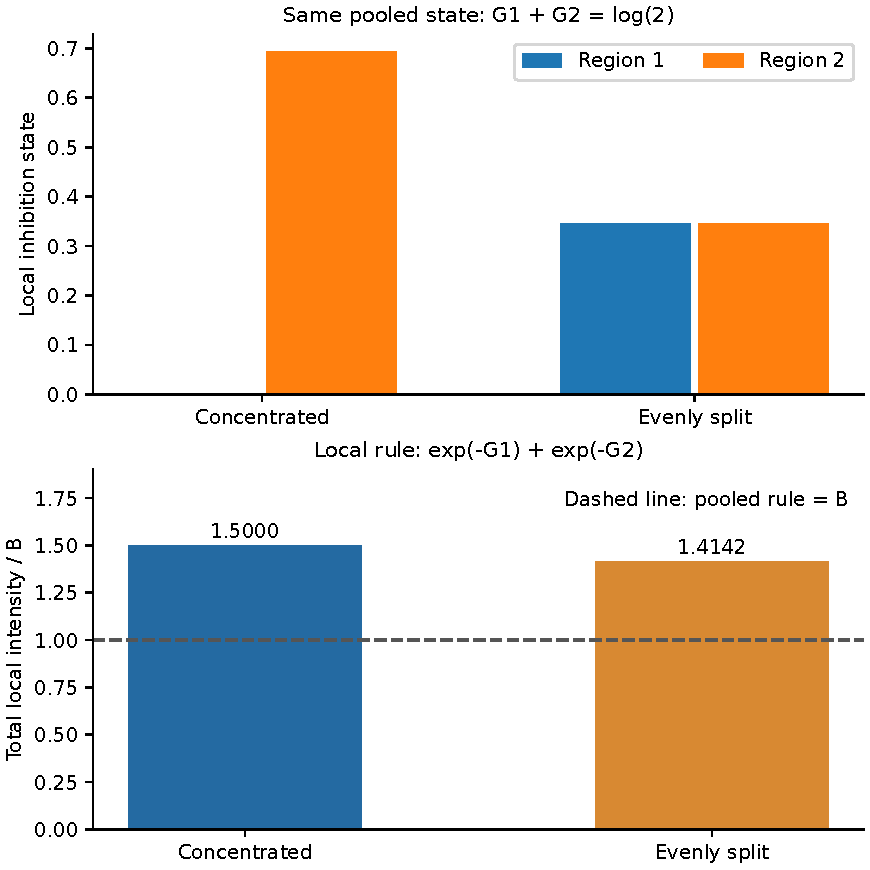
\includegraphics[width=0.85\linewidth]{pooling.pdf}
\caption{The same total depletion can have different local aggregate backgrounds. A pooled feature discards the regional allocation needed to distinguish these states. The comparison is conditional algebra, rather than an explanation of an observed predictive loss.}
\label{fig:pooling}
\end{figure}

\begin{remark}[A conditional failure of closure under pooling]
\label{prop:regional_nonclosure}
For finitely many regions, fix $B_k\geq0$ with $B_+=\sum_kB_k>0$, nonnegative depletions $G_k$, and $\eta>0$. The local aggregate background and the pooled recipe are
\begin{equation}
 J_{\mathrm{local}}=\sum_k B_k e^{-\eta G_k},
 \qquad
 J_{\mathrm{pooled}}=B_+e^{-\eta\sum_kG_k}.
\end{equation}
The local aggregate has an effective depletion
\begin{equation}
 G_{\mathrm{eff}}=-\frac1\eta\log\left(\sum_kp_ke^{-\eta G_k}\right),
 \qquad p_k=\frac{B_k}{B_+},
 \label{eq:effective_depletion}
\end{equation}
which generally depends on the regional allocation of depletion, the background shares and $\eta$. There exist two-region backgrounds for which no function of total depletion alone, including a single rescaling of $\eta$, represents this aggregate for all regional histories. This is a failure of closure of the model class, rather than a claim that every regional configuration fails to pool.

The expression for $G_{\mathrm{eff}}$ follows by factoring $B_+$ from $J_{\mathrm{local}}$ and taking the logarithm. To show the loss of information, take two equal positive backgrounds $B$ and fix $g>0$. The histories $(G_1,G_2)=(0,g)$ and $(g/2,g/2)$ both have total depletion $g$. Their local aggregates are respectively $B(1+e^{-\eta g})$ and $2Be^{-\eta g/2}$. Their difference is
\begin{equation}
 B\bigl(1-e^{-\eta g/2}\bigr)^2>0.
\end{equation}
Every recipe using only $B_+=2B$ and $G_1+G_2=g$ gives the same value on both histories, for any common choice of its inhibition coefficient. It cannot represent both distinct local aggregates.
\end{remark}



Some configurations admit pooling or rescaling; this conditional algebra supplies no empirical explanation of the observed triggering-only advantage. A regional point-process model must declare its filtration and cross-region triggering, and its likelihood must include quiet-region compensators as well as event terms. Chapter~\ref{ch:nz-spatial} reports the completed comparisons under matched observational measures.

\chapter{Finite-History Likelihood Identities and Response Tools}\label{chap:inference}\label{ch:inference}

The marked likelihood provides the common bridge from structural and visibility questions to fitted inference. It records event times, pre-event intensities, the complete observation window, and the mark factors under the same mark model. Likelihood geometry can then be separated into three questions: whether a score direction has finite second moment, whether amplitude profiling gives a well-defined finite-history optimization, and how the rejection probability of a calibrated rule responds when the generating inhibition changes.

\section{The full marked likelihood and a score bound}

For an observed marked history \((T_i,Q_i)_{i=1}^{N(T)}\), write \(G_i=G_s(T_i-)\) and \(H_i=H_e(T_i-)\), so the event at \(T_i\) is excluded from both. With the common mark density \(p_Q\),
\begin{equation}
\ell(\vartheta,\eta)
=
\sum_{i=1}^{N(T)}
\log\left\{B(T_i)e^{-\eta G_i}+nH_i\right\}
-\int_0^T\left\{B(t)e^{-\eta G_s(t)}+nH_e(t)\right\}\dif t
+\sum_{i=1}^{N(T)}\log p_Q(Q_i).
\label{eq:full-likelihood}
\end{equation}
Every event term uses its pre-event stress and trigger history, the time integral covers the full horizon, and no first event is deleted. The mark sum belongs to the full likelihood. The first two terms form its event-time contribution, evaluated on the observed marked history; they are not the marginal time-only likelihood. The mark sum cancels in a contrast only when both candidates evaluate the same marks under the same mark law and support; it is constant in ground-rate coordinates when that mark law is held fixed. Ground-rate equality without equality of mark laws is insufficient for equality of marked likelihoods. The likelihood is conditioned on the declared starting history, rather than on the observed count.

For example, let a magnitude excess \(Q\ge0\) have exponential density \(\beta e^{-\beta Q}\), and let
\[
\kappa(Q)=(1-r)e^{r\beta Q},\qquad 0\le r<1.
\]
Then \(\E \kappa=1\), and the raw triggering amplitude is
\(n(1-r)e^{r\beta Q}\). Changing \(\beta\) while holding \(r\) fixed changes both the future mark distribution and the raw productivity exponent. To preserve a raw law \(C e^{cQ}\) on the observed history under a changed \(\beta'\), one must instead use
\[
r'=c/\beta',\qquad n'=C/(1-r'),
\]
subject to \(\beta'>c\) and the branching constraints. This can preserve the event-time likelihood contribution evaluated on the observed marked history; it does not preserve the full marked law. A mark-only estimate from a training prefix is also not automatically the joint marked-process maximum-likelihood estimate, since the ground-rate term can depend on \(\beta\) through productivity.

For fixed nuisance parameters, the inhibition score is
\begin{equation}
U_\eta=\ell_\eta
=\int_0^T
-\frac{B(t)e^{-\eta G_s(t)}G_s(t)}
{B(t)e^{-\eta G_s(t)}+nH_e(t)}
\left\{\dif N(t)-\lambda_\eta(t)\dif t\right\}.
\label{eq:eta-score}
\end{equation}
At \(\eta=0\), this is the score for the declared boundary direction, with the ordinary Hawkes law as reference. The next bound shows that raw heavy-tailed marks need not imply an infinite variance for this particular intensity-weighted score.

\begin{proposition}[Restricted finite score variance]
\label{prop:score_bound}
On \([0,T]\), with empty initial history and \(\eta\geq0\), let \(0<B(t)\le B_{\max}<\infty\), \(0<n<1\), let \(\kappa>0\) almost surely with \(\E \kappa=1\), and let \(h_e\) be normalized with \(h_e(u)>0\) for \(0<u\le T\). Assume the same parents contribute to \(G_s\) and \(H_e\), with almost surely finite nonnegative mark transforms and nonnegative \(\Phi_s\), \(C_T=\int_0^T\Phi_s(u)^2/h_e(u)\,\dif u<\infty\), and \(m=\E [g(Q)^2/\kappa(Q)]<\infty\). Then the score \eqref{eq:eta-score} is square integrable and its predictable variance is
\[
\E _\eta U_\eta^2
=
\E _\eta\int_0^T
\frac{(B e^{-\eta G_s}G_s)^2}{\lambda_\eta}\,\dif t
\le
\frac{B_{\max}^2}{n}C_T\,\E _\eta N(T)m<\infty.
\]
\end{proposition}

\begin{proof}
The normalized subcritical Hawkes envelope gives \(\E_\eta N(T)\leq\mathcal B/(1-n)<\infty\), where \(\mathcal B=\int_0^T B(t)\,\dif t\). Since \(\lambda_\eta\geq nH_e\) and \(Be^{-\eta G_s}\leq B_{\max}\), Lemma~\ref{lem:weighted_history} bounds the expected bracket by
\[
\E_\eta\int_0^T\frac{(Be^{-\eta G_s}G_s)^2}{\lambda_\eta}\,\dif t
\leq\frac{B_{\max}^2}{n}\E_\eta\int_0^T\frac{G_s^2}{H_e}\,\dif t
\leq\frac{B_{\max}^2}{n}C_Tm\E_\eta N(T).
\]
The score is therefore an \(L^2\) compensated-counting martingale with the stated variance. More generally the same argument works for \(n>0\) if a finite mean count is supplied separately; subcriticality is the sufficient count control used here.
\end{proof}

Raw \(\E  g^2\) or \(\E \kappa^2\) may be infinite while the intensity-weighted ratio has finite moment. Positive \(n\) and matched triggering parents supply the required comparison history; the bound is not uniform as \(n\downarrow0\) or as the kernel-ratio integral grows.

\paragraph{Example for the declared temporal, positive-productivity mark law.}
For \(Q\sim\operatorname{Exp}(\beta)\),
\(g(Q)=e^{\gamma(Q-1)}\) and \(\kappa(Q)=(1-r)e^{r\beta Q}\),
where \(\gamma=\tfrac34\log 10\) is the local stress-mark exponent,
distinct from the auxiliary response gain in Chapter~\ref{ch:stability}.
The magnitude-six reference factor is included in \(g\); the outer
branching coefficient \(n\) is not included in \(\kappa\). Then
\[
  \E\!\left[\frac{g(Q)^2}{\kappa(Q)}\right]
  =\frac{e^{-2\gamma}}{1-r}
    \frac{\beta}{\beta(1+r)-2\gamma},
  \qquad \beta(1+r)>2\gamma.
\]
At the declared synthetic values \(\beta=2.849401764894274\) and \(r=0.7\),
the denominator is approximately \(1.390105\), giving
\(m\approx 0.216065\). Although both first moments are finite,
\(2\gamma>\beta\) and \(2r\beta>\beta\), so
\(\E[g(Q)^2]=\E[\kappa(Q)^2]=\infty\).
The finite weighted moment verifies this mark condition in Proposition~\ref{prop:score_bound},
not all its other hypotheses by itself. The positive-triggering,
matched-parent, finite-horizon and kernel-ratio conditions remain essential to that bound;
the bound is not uniform near the simultaneous zero boundary, and
no joint Fisher-information, central-limit or Wilks conclusion follows.

\paragraph{Which fitted directions inherit the mark bound.}
The preceding calculation is specific to its declared productivity ratio. In S02, the matched M2 candidate sets \(r=0\) but retains \(g(Q)=e^{\gamma(Q-1)}\); hence its ratio moment is \(\E g^2=\infty\) at the declared mark rate. In the spatial LI+ controls of Section~\ref{sec:s04-expanded}, the transform is instead \(g_+(Q)=e^{\gamma Q}\), with \(\beta=2\) and \(r=0.7\). Its ratio moment is infinite because \(\beta(1+r)<2\gamma\). Original unit-mark LI does not share this stress-mark obstruction. These statements concern ideal exponential mark laws. The executable calculation at \path{experiments/methodological_audit/moments.py} records the transforms, moment inequalities and source identities.

Failure of a sufficient upper bound is not by itself a divergence proof. The following argument supplies one for the relevant unstopped null laws with bounded kernels.

\begin{proposition}[A positive-triggering null obstruction]
\label{prop:null-score-obstruction}
Under the uninhibited temporal law, suppose the history starts empty, \(B\) is positive continuous and bounded on the finite horizon, \(0<n<1\), marks are fresh and independent with \(\E\kappa=1\) and \(\E g<\infty\), the normalized trigger kernel is bounded, and the nonnegative stress kernel is continuous with \(\Phi_s(0)=1\). If \(\E[g^2/(1+\kappa)]=\infty\), the immigrant-only null score has infinite second moment.
\end{proposition}
\begin{proof}
Condition on the first event time \(S=s\) in an early interval of positive probability and its mark \(Q=q\), allowing all later immigrants and descendants. On a later interval of positive length, the first parent's contribution gives \(G_s(t)^2\ge c\,g(q)^2\). The branching construction and fresh marks bound the expected total productivity of that parent's cluster by \(\kappa(q)/(1-n)\); future immigrant clusters contribute a finite bound independent of \(q\). Boundedness of the trigger kernel therefore gives \(\E[H_e(t)\mid S=s,Q=q]\le C(1+\kappa(q))\). Positivity of \(B\) and Jensen's inequality yield, on this interval,
\[
\E\!\left[\left.\frac{B(t)^2G_s(t)^2}{B(t)+nH_e(t)}
        \right|S=s,Q=q\right]
\ge c'\frac{g(q)^2}{1+\kappa(q)}.
\]
Integration over the first mark and that interval makes the expected bracket infinite. Meanwhile, \(\E g<\infty\), the finite mean count and bounded stress kernel imply \(\E\int_0^T B G_s\,\dif t<\infty\), so the compensated score is an integrable martingale. A square-integrable terminal score would imply finite expected bracket, a contradiction.
\end{proof}

The same argument applies on a finite spatial domain when the trigger density is bounded and the background and first-parent stress kernel have positive lower bounds on a time--space region of positive measure. The ideal spatial Omori null with positive temporal offset satisfies these conditions, as does the finite-mixture M2 candidate under its own fresh-mark null. For the exponential productivity above, \(1+\kappa\) and \(\kappa\) have equivalent tails, so the spatial LI+ ratio divergence gives the claimed null obstruction. For M2, \(\kappa=1\). This proof does not condition on absence of descendants: at positive triggering that condition would tilt the first mark's law. Nor does it identify the exact Mittag--Leffler or persistent-mark S02 generators with the finite-mixture candidate.

At the simultaneous boundary \(n=\eta=0\), the conclusion can fail. Take a constant Poisson background \(B>0\), marks \(Q\sim\operatorname{Exp}(\beta)\), and \(g(Q)=e^{\gamma(Q-1)}\) with \(\gamma<\beta\le2\gamma\). The first stress-mark moment is finite while the second is infinite. For one exponential relaxation mode of rate \(k>0\), the resulting positive shot noise has a stationary version of mean \(B\E g/k\); copies with the same future points and marks have differences that decay exactly as \(e^{-kt}\). Thus a first-moment stable state process is compatible with the following score irregularity. On the positive-probability event of exactly one event at \(S<T\), the pre-event stress is zero and the score contribution has the form
\[
U_0=g(Q)\int_S^T B(t)\Phi_s(t-S)\,\dif t.
\]
The fresh mark is independent of that event configuration, and the integral is strictly positive on a positive-probability set of \(S\). Hence the score has infinite second moment. At positive \(\eta\), even with \(n=0\),
\[
\frac{(G_sB e^{-\eta G_s})^2}{\lambda_\eta}
\le B G_s^2e^{-\eta G_s}
\le\frac{4B}{e^2\eta^2},
\]
so integrable \(B\) controls the score bracket without a raw second mark moment. This regularization is not uniform as \(\eta\downarrow0\) and does not establish null-boundary asymptotic theory.

\paragraph{Total attenuation and positive generating inhibition.}
For the separate family \(\lambda_\eta=(B+nH_e)e^{-\eta G_s}\), the fixed-nuisance score and its null expected predictable bracket are
\[
U_{\eta,\mathrm{total}}
=-\int_0^T G_s\,(\dif N-\lambda_\eta\,\dif t),
\qquad
I_{\mathrm{total}}(0)=
\E_0\int_0^T G_s^2(B+nH_e)\,\dif t.
\]
The immigrant-only ratio bound does not apply. A first parent's background contribution requires \(\E g^2<\infty\), and its same-parent stress--trigger contribution, where the kernels overlap and \(n>0\), requires \(\E[g^2\kappa]<\infty\). For \(g(Q)=C e^{\gamma Q}\) and the exponential productivity above, these conditions respectively require \(2\gamma<\beta\) and \(2\gamma+r\beta<\beta\). Both fail for the spatial LI+ law. Thus its expected null bracket diverges. These diagonal conditions are necessary obstructions, not a sufficient theorem for the cross-parent terms. Even absolute first-moment control involves \(\E[g\kappa]\), requiring \(\gamma+r\beta<\beta\); without an integrability argument, an infinite expected bracket should not be equated with an ordinary terminal-score variance.

Positive generating inhibition is different. The immigrant-only positive-\(\eta\) bound above holds regardless of the raw second mark moment. For total attenuation,
\[
G_s^2\lambda_\eta
\leq \frac{4}{e^2\eta^2}(B+nH_e),
\qquad \eta>0.
\]
The fresh-mark subcritical Hawkes envelope gives a finite expectation of the integrated right-hand side. Both families therefore have finite score brackets at each fixed positive generating \(\eta\) under these assumptions; the bounds are not uniform at the null.

A finite horizon alone does not truncate the ideal marks or counts. The implemented generators additionally use finite uniform grids, representable marks and explicit resource/numerical stopping rules. Their finite saved histories and any law conditioned on successful completion are distinct from the ideal unstopped law used above. Null moment irregularity neither proves that a positive-inhibition generating score is irregular nor establishes the cause of held-out losses, selected parameter values or optimizer behavior.

Finite score variance alone is not a central limit theorem. It also does not establish differentiability in quadratic mean for the full searched model or a regular information matrix at the boundary. This distinction is visible in the pathwise negative Hessian at the null:
\[
-\ell_{\eta\eta}(\vartheta,0)=A_T^{(2)}-C_T^{(2)},\qquad
A_T^{(2)}=\int_0^T B G_s^2\,\dif t,\qquad
C_T^{(2)}=\sum_i\frac{B(T_i)G_i^2 nH_i}{\lambda_0(T_i)^2}.
\]
For example, suppose \(B\) is continuous and positive, \(\Phi_s\) is continuous with \(\Phi_s(0)=1\), and \(\E g(Q)^2=\infty\). Let \(S\) be the first event time. Its null density on \((0,T)\) is \(B(s)\exp\{-\int_0^sB(v)\,\dif v\}\), and its fresh mark is independent of \(S\). The contribution of that first parent gives
\[
A_T^{(2)}\geq g(Q_1)^2\int_S^T B(t)\Phi_s(t-S)^2\,\dif t
\quad\text{on }\{S<T\}.
\]
The integral is strictly positive, so Tonelli yields \(\E_0 A_T^{(2)}=\infty\). This applies to the displayed exponential-mark example whenever \(2\gamma\geq\beta\). Under Proposition~\ref{prop:score_bound}'s additional hypotheses, define the finite null score bracket mean
\[
I_{\eta\eta}^{(0)}=\E_0\int_0^T\frac{B^2G_s^2}{\lambda_0}\,\dif t<\infty.
\]
Fresh-event compensation and the nonnegative integrand identity
\[
BG_s^2=\frac{BG_s^2nH_e}{\lambda_0}
       +\frac{B^2G_s^2}{\lambda_0}
\]
then imply \(\E_0 C_T^{(2)}=\infty\) as well. Thus taking the expectations of the two Hessian components separately produces an undefined \(\infty-\infty\), not a justified information identity. This fact alone does not determine integrability of their pathwise difference; cancellation would need its own argument. Finite score variance cannot be used as permission for that termwise interchange.

\section{Nuisance projection and local information}

Suppose the relevant scores are square integrable. Define the ensemble inner product
\[
\langle f,h\rangle_0
=
\E _0\int_0^T\lambda_0(t)f(t)h(t)\,\dif t.
\]
For a nuisance parameter \(\zeta\), the score integrand is
\(f_\zeta=\partial_\zeta\lambda_0/\lambda_0\). If the nuisance scores span a closed subspace, the residual after projecting \(f_\eta\) onto that subspace is the efficient-score integrand. In finite nonsingular notation,
\[
I_{\eta\mid\zeta}
=
I_{\eta\eta}-I_{\eta\zeta}I_{\zeta\zeta}^{-1}I_{\zeta\eta}
\le I_{\eta\eta}.
\]
When nuisance scores are redundant, a generalized inverse and its range condition replace the ordinary inverse.

This projection gives a quantitative meaning to masking by fitted background and triggering. Slowly varying depletion can resemble a background trend, while post-event depletion can resemble a triggering scale or productivity. It also shows why effective information is an ensemble object: it requires integrability and a reference law, not merely the algebra of one fixed path. At \(\eta=0\), the information contributed by an independently parameterized stress-kernel direction is zero, because
\(\partial_\theta\lambda=-\eta B e^{-\eta G_s}\partial_\theta G_s\).
An \(O(\eta^2)\) information statement away from zero requires a justified uniform moment bound for that derivative; the zero first derivative alone is not enough.

A related calculation can be made on one fixed reference path without the ensemble expectation. For \(B=\exp(a+d x_{\mathrm{trend}})\), the four null log-intensity directions are
\[
s_a=\frac B{\lambda_0},\quad
s_d=\frac{x_{\mathrm{trend}}B}{\lambda_0},\quad
s_n=\frac{H_e}{\lambda_0},\quad
s_\eta=-\frac{BG_s}{\lambda_0}.
\]
The realized Gram matrix \(J_{ij}=\int_0^T\lambda_0s_is_j\,\dif t\) is positive semidefinite. Its residual inhibition norm after projecting on \((s_a,s_d,s_n)\) is the minimum of
\(\int\lambda_0(s_\eta-b_as_a-b_ds_d-b_ns_n)^2\dif t\).
If \(G_s=c_0+c_1x_{\mathrm{trend}}+c_2H_e/B\), that residual is exactly zero. This algebra explains how depletion can resemble a fitted level, trend and triggering component.

On two frozen reference paths, the archived residual/raw squared-norm ratios were approximately \(10.82\%\) and \(3.26\%\). These are two realized-path projections, rather than estimates of ensemble Fisher information. The paths and their calibrations differ; their ordering does not establish that greater exposure reduces expected information. Additional score directions can only reduce the residual for the same path and inner product, but no power decomposition follows from that projection fact.

\section{Conditional amplitude profiling}

Fix one observed marked history and fix the trend coefficient \(d\) and inhibition \(\eta\). Put
\[
q_i=\exp\{d x_{\mathrm{trend}}(T_i)-\eta G_i\},
\qquad
c_i=nH_i,
\qquad
J=\int_0^T\exp\{d x_{\mathrm{trend}}(t)-\eta G(t)\}\,\dif t,
\]
and let \(A=\exp(a)\) with \(A\in[L,U]\), where \(L=e^{-12}\) and \(U=1\). The negative event-time contribution to the joint marked log-likelihood, omitting the common mark constant and writing \(K=\int_0^T H_e(t)\,\dif t\), so that \(nK\) is the full-window triggering compensator, is
\begin{equation}
F(A;d,\eta)=AJ+nK-\sum_{i=1}^{N}\log(Aq_i+c_i).
\label{eq:amplitude-objective}
\end{equation}
The full horizon and all pre-event intensities are retained. The mark factors in \eqref{eq:full-likelihood} are constant in these fitted coordinates under the common mark model.

\begin{proposition}[Conditional amplitude profile]
\label{prop:amplitude}
Assume a finite history and finite event features and parameters. Let every \(c_i\ge0\), let \(K\) be finite, and require \(0<J<\infty\). The specified finite-mode observation window satisfies these conditions when \(x_{\mathrm{trend}}\) is bounded and all recorded marks are finite. Then \eqref{eq:amplitude-objective} has a unique minimizer on \([L,U]\):
\begin{enumerate}
\item if \(F_A(L)\ge0\), the minimizer is \(L\);
\item otherwise, if \(F_A(U)\le0\), the minimizer is \(U\);
\item otherwise, the unique interior root of the continuous strictly increasing \(F_A\) is the minimizer.
\end{enumerate}
If \(N=0\), the unique minimizer is \(L\).
\end{proposition}

\begin{proof}
Ordinary finite-sum differentiation gives
\[
F_A=J-\sum_{i=1}^{N}\frac{q_i}{Aq_i+c_i},
\qquad
F_{AA}=\sum_{i=1}^{N}
\left(\frac{q_i}{Aq_i+c_i}\right)^2.
\]
For \(N\ge1\), \(q_i>0\), so \(F_{AA}>0\) and \(F_A\) is strictly increasing and continuous on the compact interval. If its endpoint values place zero inside the interval, it has one root, and the sign change from negative to positive identifies that root as the unique minimizer; endpoint cases place the minimizer at the corresponding boundary. If \(N=0\), then \(F(A)=AJ+nK\) is strictly increasing because \(J>0\), so the lower endpoint is the unique minimizer.
\end{proof}

The amplitude result is a finite-history optimization fact, not a global fit certificate. Convexity in \(A\) does not make the profiled surface \(V(d,\eta)=F(A_*(d,\eta);d,\eta)\) convex in \((d,\eta)\). A finite grid or local search establishes only its declared numerical search outcome.

For \(a=\log A\), set \(p_i=Aq_i/(Aq_i+c_i)\). Then
\[
g(a)=F_a=AJ-\sum_i p_i,
\qquad
g'(a)=AJ-\sum_i p_i(1-p_i),
\]
and \(g\) need not be monotone even though \(F_A\) is increasing in \(A\). A bracketing method for \(a\) can rely on continuity and endpoint signs, not on monotonicity of \(g\). At an interior root the exact balance is
\[
AJ=\sum_i p_i.
\]
The curvature identity in log amplitude is
\[
F_{aa}=\sum_i p_i^2+R,
\qquad
R=AJ-\sum_i p_i.
\]
Thus at the balanced root, the negative log-likelihood satisfies
\(F_{aa}=\sum_i p_i^2\), while the log-likelihood \(\ell=-F\) satisfies
\(\ell_{aa}=-\sum_i p_i^2\). At an approximate root, the balance residual \(R\) must be added to \(\sum_i p_i^2\); it is not exact curvature at that numerical point. In a region where the optimizing amplitude is interior, profile differentiation also gives
\[
V_d=AJ_x-\sum_i x_{\mathrm{trend}}(T_i)p_i,
\qquad
V_\eta=-AJ_G+\sum_i G_ip_i,
\]
where \(J_x\) and \(J_G\) integrate \(x_{\mathrm{trend}}(t)\) and \(G(t)\) against the background weight. Here \(J_x=\int_0^Tx_{\mathrm{trend}}(t)e^{dx_{\mathrm{trend}}(t)-\eta G(t)}\dif t\) and \(J_G=\int_0^TG(t)e^{dx_{\mathrm{trend}}(t)-\eta G(t)}\dif t\). At fixed \(d\), implicit differentiation in an interior-amplitude region gives

\[
\frac{\partial a_*}{\partial\eta}
=\frac{AJ_G-\sum_iG_ip_i(1-p_i)}{\sum_i p_i^2}.
\]
The numerator has no universal sign. An amplitude curve that also refits trend has a different total derivative. The identity \(AJ=\sum_i p_i\) equates integrated fitted background with event-wise background mixture weights; these weights are not observed physical parent labels or a stationary balance law. With empty prehistory and positive background, the first event has \(c_1=0\), so \(p_1=1\). No initial quiet interval or first event can be discarded from this argument.

These are local envelope and implicit formulas. Active endpoint transitions require one-sided treatment, and none of them implies that every starting point reaches the global profile minimum.

Stable evaluation also matters for the conditional proof. In logarithmic coordinates compute \(\log\lambda_i\) by a log-sum-exp of \(a+\log q_i\) and \(\log c_i\). When \(c_i=0\), the mathematically positive background gives \(p_i=1\), even if exponentiating \(\log q_i\) underflows. A numerical zero is not evidence that the exact objective is flat. The same amplitude algebra holds with positive quadrature weights, but agreement between quadrature orders at selected points is a numerical sensitivity check rather than a rigorous global integration bound.

\section{Boundary hypotheses and calibration}
\label{sec:boundary_calibration}

Feedback detection and testing equality of memories are different tasks. The first compares \(\eta=0\) with an active alternative; the second compares shared and separate stress/trigger families while permitting inhibition. At zero feedback, an independently varied stress-kernel parameter disappears from the observed law. Together with the one-sided constraint \(\eta\ge0\), this produces a nonregular null: there is a nuisance parameter present only under the alternative. A fixed-kernel boundary formula cannot automatically calibrate a maximization over stress kernels and fitted nuisances. The general difficulty is discussed by \citet{Davies1977}; the regularity conditions of boundary likelihood theory, including those in \citet{SelfLiang1987}, need their own verification here.

A calibration recipe must match the complete statistic actually computed. Under a fitted null, this means simulating new marked catalogues, refitting the allowed nuisance parameters under both candidates, repeating the declared kernel search and using the same failure and selection rules. A reference distribution for one nuisance block cannot be substituted for another. Such a plug-in procedure is a proposed finite-sample method; the present score bounds do not prove its uniform validity over a composite null or near weak identification. Non-rejection of shared memory cannot confirm that restriction without evidence that meaningful separate-memory alternatives are distinguishable.

The distinction between supplied and estimated nuisances is equally substantive. A likelihood ratio between two fully specified laws addresses a simple testing problem. A composite null can change its background and other permitted parameters, admitting alternative explanations that the simple null excludes. Superior calibrated detection with supplied generating values therefore does not measure purely avoidable fitting inefficiency. It combines different statistical questions with different procedures; neither an arbitrary optimizer improvement nor fixing real-data nuisance values without justification is guaranteed to recover the supplied-law performance.

\section{Response of a calibrated fixed-rule test}

Calibrated inference starts with a complete-data decision rule rather than with a particular fitted parameter value. Let \(I(\mathcal H)\in\{0,1\}\) be a fixed bounded measurable rejection indicator defined on every admissible marked history. The reference bank, tuning and model-selection procedure, critical threshold, treatment of empty histories, and any auxiliary randomization law are fixed independently of the true generating inhibition. The rule may estimate nuisances or select a model from the data, because these operations are part of the same measurable mapping from history to \(\{0,1\}\); what is held fixed is the rule as the generating \(\eta\) varies. Define
\[
p(\eta)=\E _\eta I(\mathcal H).
\]

\begin{proposition}[Positive-inhibition response of a fixed rule]
\label{prop:power_response}
Fix empty history, a common fresh mark law with finite nonnegative transforms, \(\E \kappa=1\), \(0\le n<1\), nonnegative kernels bounded on the finite window with normalized \(h_e\), and a deterministic nonnegative background with \(\mathcal B=\int_0^TB(t)\dif t<\infty\). Hold all these generating nuisances fixed as \(\eta\) varies. Then \(p(\eta)\) is continuously differentiable for \(\eta>0\), and
\[
p'(\eta)=\E _\eta[I(\mathcal H)S_\eta]
=\mathrm{Cov}_\eta(I(\mathcal H),S_\eta).
\]
Moreover,
\[
|p'(\eta)|
\le
\frac{2\sqrt{\mathcal B\,p(\eta)(1-p(\eta))}}{e\eta}
\le
\frac{\sqrt{\mathcal B}}{e\eta}.
\]
If in addition the fixed generating ingredients satisfy Proposition~\ref{prop:score_bound}, put
\[
K_T=\frac{B_{\max}^2C_Tm\mathcal B}{n(1-n)}.
\]
Then the stronger bound
\[
|p'(\eta)|\leq\sqrt{K_Tp(\eta)(1-p(\eta))}
\leq\frac{\sqrt{K_T}}2,\qquad \eta>0,
\]
is uniform in positive \(\eta\) with those ingredients fixed. It does not assert existence of \(p'(0)\).
\end{proposition}

\begin{proof}
Let \(P_0\) be the noninhibited Hawkes law. Its mean count is at most \(\mathcal B/(1-n)\), and it dominates each inhibited construction. On a finite path the likelihood ratio is
\[
L_\eta=\exp\left\{\int_0^TB(1-e^{-\eta G_s})\dif t\right\}
\prod_i\frac{Be^{-\eta G_i}+nH_i}{B+nH_i}\le e^{\mathcal B}.
\]
At actual event times the reference intensity is positive almost surely; where both intensities vanish away from events, set their likelihood ratio to one. The stopped density martingale is uniformly bounded and hence defines the changed law. Its score \(S_\eta=\partial_\eta\log L_\eta=U_\eta\) satisfies
\[
\E _\eta S_\eta=0,\qquad
\E _\eta S_\eta^2\le\frac{4\mathcal B}{e^2\eta^2},
\]
by the positive-inhibition bracket bound, without a raw stress-mark second moment.

For clarity, write
\[
\begin{aligned}
 \mathcal B&=\int_0^T B(t)\,\dif t,
 &J_\eta&=\int_0^T B(t)(1-e^{-\eta G_s(t)})\,\dif t,\\
 \varrho_i(\eta)&=\frac{B_i e^{-\eta G_i}+c_i}{B_i+c_i},
 &c_i&=nH_i\geq0,
\end{aligned}
\]
where $B_i=B(T_i)$ and $G_i,H_i$ are the pre-event features. Then
$L_\eta=e^{J_\eta}\prod_i\varrho_i(\eta)$, with $0\leq \varrho_i\leq1$ and
$0\leq J_\eta\leq\mathcal B$. At actual reference-law events
$B_i+c_i>0$ almost surely. On a compact positive interval
$\eta\in[\eta_-,\eta_+]$, direct differentiation gives
\[
 |\varrho_i'(\eta)|
 =\frac{B_i}{B_i+c_i}G_i e^{-\eta G_i}
 \leq\frac{1}{e\eta_-},
 \qquad
 |J_\eta'|\leq\frac{\mathcal B}{e\eta_-}.
\]
The product rule, without division by any $\varrho_i$, therefore yields
\[
\begin{aligned}
 |\partial_\eta L_\eta|
 &\leq e^{J_\eta}\left(
 |J_\eta'|\prod_i\varrho_i+
 \sum_i |\varrho_i'|\prod_{j\ne i}\varrho_j\right)\\
 &\leq\frac{e^{\mathcal B}(\mathcal B+N(T))}{e\eta_-}.
\end{aligned}
\]
The same bound applies to $|\partial_\eta(L_\eta I)|$ for the fixed bounded
indicator. It is integrable under the reference law because
$\E _0N(T)\leq\mathcal B/(1-n)$. The bound is for the derivative of
$L_\eta$, not its logarithm. The finite-path derivative is continuous in $\eta$. Dominated convergence gives
\(p'(\eta)=\E _0[I\partial_\eta L_\eta]=\E _\eta[IS_\eta]\).
No derivative of the data-dependent fitted outputs is taken: \(I\) is the same mapping on every history. The mean-zero score gives the covariance identity. Cauchy--Schwarz with \(\mathrm{Var}(I)=p(1-p)\) gives the general bounds. Under the additional weighted-moment hypotheses, Proposition~\ref{prop:score_bound} and \(\E_\eta N(T)\leq\mathcal B/(1-n)\) instead give \(\E_\eta S_\eta^2\leq K_T\); the same covariance inequality proves the uniform bound.
\end{proof}

The covariance has no proved sign. Stronger generating inhibition need not increase detection probability for a particular calibrated rule. The general positive-\(\eta\) estimate gives local differentiability and moment control but is not uniform as \(\eta\downarrow0\). The stronger bound needs positive triggering and the finite weighted-history moment; it bounds the positive-parameter slopes but supplies neither monotonic power nor null-boundary asymptotic calibration. Unknown, failed, capped, or otherwise unresolved computational outcomes remain unknown; they must not be recorded as nonrejections. Conditioning on completed cases estimates a different functional from the unconditional \(p(\eta)\) defined by the fixed rule.

The proposition also does not compare a simple hypothesis with a known generating law to a composite hypothesis whose nuisances are fitted. Those are different operating characteristics, with different permitted null explanations and decision rules. An oracle that knows the nuisance values and a composite rule that estimates them are not the same test function, so their performance gap is not by itself pure fitting waste.

\section{Scope and unresolved inference}

Taken together, the results separate four questions. Exact marked-law equality shows that zero feedback leaves a separately varied stress kernel unidentified; the restricted active-inhibition experiment can identify the inhibition parameter and kernel in an idealized full-law sense; the restricted score can remain square integrable even when raw mark moments diverge; and a calibrated fixed rule has a local covariance response at positive inhibition. Amplitude profiling adds a unique conditional optimization in \(A\), while leaving the remaining trend--inhibition surface without a global certificate.

These statements do not imply a Wilks law, a general Fisher-information theorem, likelihood-ratio asymptotics at \(\eta=0\), uniform validity near the boundary, a necessary detection threshold, or a finite-sample power result. They also provide no new numerical evidence and do not replace a specified calibration procedure by a general asymptotic claim. The unresolved inference is therefore explicit: structural identification in a restricted family is not practical detectability; finite score variance is not a distributional approximation; conditional amplitude uniqueness is not global identifiability; and a signed response formula for a fixed rule is not a theorem that stronger inhibition creates a more powerful test.

\chapter{Experimental Design, Sequential Conditional Scoring, and Audit Protocols}\label{chap:design}
\label{ch:design}

This chapter specifies the finite-history experiment used to study detection of the diagnostic inhibition term. The quantity of primary interest is a diagnostic inhibition parameter, \(\eta\), not the physical loading parameter of the original process model. The distinction is substantive. Within the diagnostic family, a positive \(\eta\) suppresses the background contribution after the specified history feature is represented. It does not identify the original physical loading parameter, nor does it establish a unique physical mechanism. The experiment is therefore an inference study about a class of fitted laws, not a reconstruction of a complete physical loading history.

The synthetic construction is model-correct relative to the laws it generates: histories are produced from the stated marked point-process model, evaluated under that model, and compared without introducing an external observation model. Geography, changing observation practices, and missing parents are deliberately omitted. Consequently, agreement or disagreement among procedures on these histories measures behavior within a specified filtration and law class. It cannot by itself establish that the same procedures are adequate for a catalogue affected by spatial heterogeneity, reporting changes, or genealogical incompleteness.

\section{The diagnostic law and its history}

For a history \(\mathcal H_t\), let
\begin{equation}
\lambda_\eta(t)
=
\exp\!\left\{a+d\left(\frac{2t}{T}-1\right)\right\}
\exp\{-\eta G_s(t)\}
+
nH_e(t),
\label{eq:experiment-intensity}
\end{equation}
where
\[
B(t)
=
\exp\!\left\{a+d\left(\frac{2t}{T}-1\right)\right\}.
\]
Here \(a\) controls the background level, \(d\) the linear trend in transformed time, \(n\) the additive triggering scale, and \(\eta\) the diagnostic inhibition of marked stress memory. The feature \(G_s(t)\) is a nonnegative marked stress-memory feature, while \(H_e(t)\) is a normalized marked triggering feature. The interpretation of \(\eta\) is conditional on the represented triggering process and on the specified background: it is an attenuation of the first term in \eqref{eq:experiment-intensity}, not a declaration that the physical process is governed by an equivalent coefficient.

Both \(G_s\) and \(H_e\) are functions of the strictly earlier history. If event \(i\) has time \(t_i\) and mark \(m_i\), the predictable intensity used for that event is \(\lambda_\eta(t_i-)\). The mark \(m_i\) affects later stress memory and later triggering but cannot affect the intensity immediately before its own occurrence. This timing convention prevents circular use of the event being evaluated and is essential to the likelihood interpretation below.

The numerical kernels are positive normalized finite spectral mixtures. They represent the stress and triggering responses with a finite number of modes rather than by evaluating the exact Mittag--Leffler kernel. In the shared implementation, the kernel scale parameters are \(\alpha=0.5\) and \(\tau=1\), and the normalized mixture comprises \(195\) modes. Although the modes may approximate a long-memory response, the finite mixture is itself the implemented model. For magnitude excess \(m_i=M_i-M_0\), the implemented features are
\begin{align}
 G_s(t)&=\sum_{t_i<t} e^{\gamma(m_i-1)}\Phi_s(t-t_i),
       &\gamma&=\tfrac34\log 10,\\
 H_e(t)&=\sum_{t_i<t}(1-r)e^{\beta r m_i}h_e(t-t_i).
 \label{eq:diagnostic-features}
\end{align}
The relaxation kernel has the form \(\Phi_s(u)=\sum_qw_qe^{-\rho_qu}\), with positive weights summing to one. The corresponding triggering density is \(h_e(u)=\sum_qv_q\zeta_qe^{-\zeta_qu}\), with positive weights summing to one and positive rates. Thus \(\Phi_s(0)=1\) and \(\int_0^\infty h_e(u)\,\dif u=1\). Sharing the relaxation parameters means using a common survival kernel and its negative derivative as the triggering density, rather than setting the two functions equal. The stress-mark normalization is the declared magnitude-six reference when \(M_0=5\). These formulas are explicit in \href{https://github.com/Drefetr/InhibitoryEarthquakeModels/blob/3e76a174cf4f58ce601c6c9640c4d0c11168813f/engine/iteration_20/code/restricted_history.py}{public restricted-history implementation} (\texttt{S10}) and \href{https://github.com/Drefetr/InhibitoryEarthquakeModels/blob/3e76a174cf4f58ce601c6c9640c4d0c11168813f/engine/iteration_27/code/adequacy.py}{public observed implementation} (\texttt{S17}). Conclusions therefore apply to the finite mixture that was used, not automatically to every exact infinite-mode limit.

\paragraph{Finite spectral recipe.}
For \(0<\alpha<1\) and the dimensionless rate variable $u$, the continuous representation
\citep[Eqs.~(2.12)--(2.13)]{Mainardi2014} is
\[
 E_\alpha(-t^\alpha)=\int_0^\infty e^{-ut}K_\alpha(u)\,\dif u,
 \qquad
 K_\alpha(u)=\frac{\sin(\pi\alpha)}{\pi}
 \frac{u^{\alpha-1}}{u^{2\alpha}+2u^\alpha\cos(\pi\alpha)+1}.
\]
Writing $u=e^v$ gives the log-rate density
\[
 K_\alpha(e^v)e^v=
 \frac{\sin(\pi\alpha)}{2\pi\{\cosh(\alpha v)+\cos(\pi\alpha)\}}.
\]
For the scaled relaxation $E_\alpha(-(t/\tau)^\alpha)$, the rates are
$e^v/\tau$. The following finite rule applies trapezoidal weights on the
stated log-rate grid, halves its endpoints, truncates and renormalizes.
The continuous representation and this numerical discretization are distinct;
the citation does not provide a universal likelihood- or inference-error bound.
The generating relaxation uses log rates \(v_j=0.4j\), \(j=-97,\ldots,97\), and rates \(\rho_j=e^{v_j}/\tau\) in days\(^{-1}\), with \(\alpha=0.5\) and \(\tau=1\) day. Before normalization its weights are
\[
 \widetilde w_j=\frac{0.4\sin(\pi\alpha)}{2\pi\{\cosh(\alpha v_j)+\cos(\pi\alpha)\}},
\]
with both endpoint weights halved, then \(w_j=\widetilde w_j/\sum_k\widetilde w_k\). More generally the implemented endpoint index is
\[
 J=\left\lceil\frac{1}{s}\max\left\{\frac{\log4}{\alpha},
 \frac{\log[4\sin(\pi\alpha)/(\pi\alpha\varepsilon)]}{\alpha}\right\}\right\rceil,
 \qquad s=0.4,\quad\varepsilon=10^{-8}.
\]
Thus the 195-mode count specifies the generating case, while candidate \(\alpha=0.7\) uses 137 modes with the same spectral rule. The machine-readable methods supplement supplies the rates and normalized weights. The finite triggering density remains \(h=-\Phi'\); its finite value at zero does not reproduce the exact fractional singularity.


Marks are generated with excess density
\[
f_\beta(m)=\beta e^{-\beta m},\qquad m>0,
\]
with \(\beta=2.849401764894274\). The normalized productivity factor is
\[
(1-r)e^{\beta r m},\qquad r=0.7.
\]
This normalization gives unit mean productivity at the reference scale and keeps the productivity multiplier positive. The exponential excess itself has finite moments. It is the exponential stress and productivity transforms that have finite first but infinite second moments at the declared parameters. That feature motivates bounded-indicator simulation checks rather than variance formulas or finite-information shortcuts based only on the raw marks.

\section{Generating histories and evaluating both laws}

The main generating experiment has duration \(T=24394\) days, begins with an empty prehistory, and produces random event counts. Counts are not conditioned on a target total; in particular, the design does not condition on a 913-event count. The generating nuisance parameters include
\[
a=-4.162108473051707,\qquad
d=0.23211265877958467,\qquad
n=0.5017751599706763,
\]
and the main diagnostic value is
\[
\eta=0.4885010300470942.
\]
The null experiment sets \(\eta=0\) while retaining the generating nuisance values in the null law. This is a comparison between a marked process with stress inhibition and a marked process without that inhibition, not a comparison against a law with triggering or marks removed.

The null reference bank is generated at the known simulation nuisance vector, not at an estimated null fit from each query. Thus even the procedures that estimate nuisance parameters are calibrated here against an oracle-supplied generating law. This controlled comparison isolates specified fitting procedures; it is not an implementable plug-in bootstrap for an unknown composite null, nor a test with demonstrated size uniformly over nuisance values.

\paragraph{Simulation and event clock.}
The simulator starts both modal states at zero. At each proposal it samples an exponential wait with envelope \(e^{a+|d|}+\sum_qw_qE_q\), where \(E_q\) is the current excitation state, advances and decays both modal states, and accepts with probability equal to the new predictable intensity divided by that envelope. Nonnegative inhibition bounds the background by \(e^{a+|d|}\), and excitation decays between events. Only after acceptance is a fresh exponential excess mark drawn; its productivity and stress increments then update future states. Proposals reaching the horizon add no event. The accepted clock retains the legacy compensated binary64 projection and the exact Decimal sum of sampled binary64 waits at precision 1600, together with residual coordinates and positive relative event gaps. Projected ties are retained without jitter or resampling; paired-clock likelihood evaluation uses those gaps. Unrepresentable waits, mark-transform overflow and resource caps remain explicit unresolved cases, with restart state retained.


For observed event times \(t_i\) and marks \(m_i\), the marked point-process log likelihood is
\begin{equation}
\ell(\vartheta,\eta;\mathcal H_T)
=
\sum_{i:t_i\le T}\log\lambda_\eta(t_i-)
-
\int_0^T\lambda_\eta(t)\,\dif t
+
\sum_{i:t_i\le T}\log f_\beta(m_i).
\label{eq:marked-likelihood}
\end{equation}
Evaluation uses the full predictable intensity and the full integral, including quiet exposure before, between, and after events and the terminal interval up to \(T\). It is not a count-conditional likelihood on the event times alone. When the same mark density is held fixed for both laws, the mark terms in \eqref{eq:marked-likelihood} cancel in their difference. They are present in both likelihoods; their cancellation is an algebraic consequence of the common mark law, not an omission of marks from the model.

Two comparison designs are distinguished. An oracle signed log-likelihood ratio compares two fully supplied laws. A fitted generalized statistic instead permits separate null and alternative optimizations over the nuisance parameters allowed by each procedure. The oracle therefore has additional information: it knows nuisance values that an estimation procedure must recover. This changes a simple-law comparison into a composite-law task. A contrast such as \(100\%\) detection for the known-law procedure versus roughly \(38\%\) for a fitted procedure is not, by itself, evidence of avoidable numerical inefficiency, nor does it establish the power of a hypothetical oracle for the composite problem. Estimating nuisance changes both the test statistic and its null distribution. Each procedure consequently requires its own reference calibration. In symbols, the oracle uses the signed contrast
\begin{equation}
 L_{10}=\ell(\vartheta_\star,\eta_\star;\mathcal H_T)
        -\ell(\vartheta_\star,0;\mathcal H_T),
 \label{eq:oracle-statistic}
\end{equation}
whereas a fitted procedure uses its selected maxima to form
\begin{equation}
 D=2\left\{\widehat\ell_1-\widehat\ell_0\right\}.
 \label{eq:fitted-statistic}
\end{equation}
The hats denote the declared finite fitting recipe, rather than a proof that a global maximum has been found. The oracle contrast need not be nonnegative; a fitted statistic with an exact eligible null floor is nonnegative. Their numerical scales and critical values cannot be exchanged.

\section{Reference calibration and inferential scope}

For each historical matched-law method described here, the null calibration uses \(999\) reference null history identifiers and a separate bank of \(1{,}000\) null query histories. The same reference identities are reused across methods, but each method fits and scores its own statistic on those histories. The \(150\) stronger alternative histories are also held in common across procedures. Reference histories are not scored as queries. For a query statistic \(D_q\), the reported rank probability is
\begin{equation}
p=\frac{1+\sum_{j=1}^{999}\mathbf 1\{D_j\ge D_q\}}{1000},
\qquad
\text{reject if }p\le 0.05.
\label{eq:rank-p}
\end{equation}
All ties count through the indicator, with no random tie breaking or exclusion. The add-one term and the denominator of \(1{,}000\) make the query effectively one member of a rank set containing \(999\) calibration references.

The reported summaries condition on the realized reference banks and generating law. For a procedure fixed in advance whose reference and query histories are exchangeable under the null, the rank rule has the usual finite-sample conservativeness of a Monte Carlo rank test. That ideal argument is not retrospective proof for a procedure selected and reused during the research process. Adaptive selection followed by scoring can alter both the statistic and the comparison being calibrated. The reported Clopper--Pearson intervals are nominal exact binomial summaries under fixed-bank, fixed-procedure and independent-query assumptions. They describe Monte Carlo uncertainty in query outcomes, rather than conditioning away those outcomes. They do not resample the reference bank, the generator, or the adaptive procedure-selection process. Similar realized null rejection rates therefore do not prove equal test size uniformly over a composite null.

The null value \(\eta=0\) lies on the boundary of the permitted nonnegative parameter space. The usual interior-parameter Wilks argument does not apply directly. This study uses empirical matched-null calibration rather than asserting a chi-squared reference law. The inferential calculations are based on the separately calibrated procedures and their realized reference distributions. Because each rejection decision is a bounded indicator, conditional Monte Carlo standard errors remain meaningful even when individual marked histories are heavy tailed. This does not imply that a finite joint Fisher information exists for the fitted model.

\section{Numerical controls and completed evidence}

The evaluation retains the full event clock, including extreme histories, rather than replacing generated histories with summaries. Required optimizer starts must resolve; an unresolved calculation stopped at a cap is recorded as unknown and is never converted into a non-rejection. Selected-point likelihood and intensity comparisons were checked across integration orders and backends, and direct likelihood contrasts were used where possible to reduce cancellation between nearly equal large integrals. Numerical envelopes serve as sensitivity controls for these calculations. They are not a universal quadrature bound and do not establish global maxima for an optimization.

The completed historical oracle, supplied-nuisance, estimated-background and level-only evaluations each retain all \(2{,}149\) declared histories. No failed or extreme history is removed to obtain these denominators. Reporting policies, inclusion rules, and provenance for the numerical controls are recorded in the appendix. The completed-history evaluation and its reference-calibration conventions are documented in \hyperlink{S09}{archival \texttt{S09} (recovered archive)}; the matched synthetic construction and likelihood accounting are recorded in \hyperlink{S11}{archival \texttt{S11} (recovered archive)}, and the final reporting structure is recorded in \hyperlink{S16}{archival \texttt{S16} (recovered archive)}.

\paragraph{Procedure-specific estimation.}
The completed supplied-trigger studies hold \(n,r,\beta,\alpha_e,\tau_e\) and the stress kernel fixed. The eta-only procedure uses starts \(0\) and \(0.2\) over \(\eta\in[0,3]\). The level-and-trend procedure runs two null optimizations in \((a,d)\in[-12,0]\times[-2,2]\) and selects the better null fit. It then runs two alternative optimizations from that one fit, initialized at \(\eta=0\) and \(\eta=0.2\). Thus level-and-trend has four prescribed optimizations; the two procedures together have six. Both use L-BFGS-B with \(\mathrm{maxiter}=100\), \(\mathrm{maxls}=40\), \(\mathrm{ftol}=10^{-10}\) and \(\mathrm{gtol}=2\times10^{-6}\). Failure alone enables the same-start CPU retries (line-search limits 40 then 200), followed by bounded Powell; the supplied-trigger procedures never free \(n\). Every prescribed start must resolve, the exact matching null remains eligible, and selected order 16 values are checked independently at CPU order 32 to tolerance \(10^{-4}\).
The distinct level-only procedure supplies \(d\) and profiles \(a\in[-12,0]\) for each \(\eta\). It checks 17 equally spaced \(\eta\)-values in \([0,3]\), the saved supplied-background alternative and zero, refines strict local mesh minima, and includes an 11-point profile. Its saved eligible floors and all mandatory solver returns are retained. Complete bounds, starts, stopping and recovery rules for this procedure, the historical fuller fit and the observed predictive fits are given separately in the methods supplement; none is a claim of global optimization.

\paragraph{Numerical integration and stable evaluation.}
The positive-gap history geometry retains initial and terminal quiet exposure. Within each event gap it inserts the offsets shorter than the gap from 23 geometric values spanning \(10^{-6}\) to \(10^5\) days and their 22 adjacent geometric means, then applies Gauss--Legendre order 16 on each subpanel. Selected controls use independent CPU order 32; the oracle refinement can require order 64. The triggering compensator uses the finite-mixture CDF, evaluated with \(-\operatorname{expm1}(-\rho_q u)\). Event log intensity uses a log-sum-exp evaluation, including an explicit zero-triggering branch. Each event reads the decayed pre-event state before adding its mark. The historical fuller search and observed search have separate parameter and recovery contracts in the companion specification.

\paragraph{Companion procedure specification.}
The portable methods supplement and machine-readable settings in \texttt{supplements/}
% Exact companion paths: supplements/methods_supplement.md; supplements/methods_settings.json
 distinguish the generating kernel, the historical fuller calibration, the supplied-trigger procedures, the level-only profile and the observed predictive search. They record estimated and supplied coordinates, bounds, starts, quadrature, recovery and unresolved availability limits at their respective accepted versions. The metadata arrays are deterministic evaluations of the documented mixture rule, not new event histories or refits.

The \href{https://github.com/Drefetr/InhibitoryEarthquakeModels/blob/3e76a174cf4f58ce601c6c9640c4d0c11168813f/paper/data/detection.json}{public detection summary} and the \hyperref[sec:source-supplements]{availability guide} provide public entry points. The original primary history bank and the complete executed known-law likelihood-and-rank replay are now supplied under \path{reproduction/synthetic/} and \path{reproduction/oracle/}. The replay starts from event histories and reproduces the saved oracle decisions. The original fitted-procedure records and their source reports are supplied under \path{reproduction/historical_fits/}.


\section{Sequential conditional prediction and regional cohorts}\label{sec:unified-design}

The observed comparisons use chronological training prefixes and later scored windows. Parameters, fitted mark-rate recipes and spatial nuisance choices are estimated from training information and frozen for each test window. During that window, strictly earlier observed test events enter the history. This is sequential conditional scoring: it differs from issuing a distribution for a complete future catalogue at a training cutoff. Equal timestamps are handled by the source-specific strict-history/batch convention; an event never predicts itself.

New Zealand uses the reconstructed GeoNet snapshot and its common historical targets. The baseline and primary middle stages retain the original chronological windows; constant-background and post-1980 sensitivities are separate procedures, not extra primary replications. California uses the repaired preferred-record schema with an explicit warmup interval. Its higher-magnitude sensitivity selects a different target set. Japan uses complete reported-primary magnitude records from the declared annual archives and an explicit missing-primary exclusion rule. Exact cohort sizes, time windows, warmup and training-prefix counts are retained in Chapters~\ref{ch:observed} and~\ref{ch:external}. They must not be pooled into a single denominator or repeatedly counted as fresh evidence.

Training-only spatial density selection prevents direct use of future test locations in nuisance fitting. It does not identify immigrant geography: the training density describes observed events, including clustering. Leave-one-out bandwidth selection and subsequent full-training plug-in estimation are also different operations. Shared nuisance scales in a factorial comparison mean that the result is conditional on the shared rule, not an independent full optimization of every family.

\section{Score sign, denominator and common-space checklist}\label{sec:score-audit}

Every comparison is candidate minus a named reference on common observations and a common dominating measure. The master definitions in Section~\ref{sec:master-scores} give
\[
 \Delta\ell_{\rm score}=\Delta P-\Delta E+\Delta M
 =\Delta Q+\Delta C+\Delta(P-Q)+\Delta M.
\]
The event contribution is $\Delta P$, never canonical $E$. Positive integrated exposure is subtracted; a raw archived key called \texttt{C} can denote a signed contribution or positive exposure, so the source-field crosswalk must be consulted. Quiet periods, all scored spatial cells and the terminal censor remain in the compensator. Spatial densities measured per projected square kilometre cannot be compared directly with label-only scores without a declared common-space lift.

Pooled nats per target are the sum of the window score differences divided by the sum of their test counts. An unweighted average of window-normalized differences is generally a different quantity. Fold signs, component signs and pooled signs answer different questions. The class-history mark likelihood is scored once; it is not silently assumed to cancel when the model changes the conditional class law. Neither a positive event-only contrast nor a larger location term establishes a positive complete joint score.

\section{Three separate calibration questions}

The historical nuisance ladder calibrates a procedure-specific test statistic against a matched reference bank. A separate observed in-sample exercise calibrates the no-feedback and common-memory restrictions under their fitted null laws, as reported in Chapter~\ref{ch:observed}; those conditional restriction tests are distinct from both synthetic detection and later predictive scoring. California conditional simulation instead starts from each original frozen OC state and generates complete branching futures for diagnostic coordinates. Its insertion-rank intervals, ties and audit scope are given in Chapter~\ref{ch:calibration}. That exercise does not calibrate EP and does not supply a composite boundary test for inhibition. The original LI fixed-seed histories are engineering/regime controls. The expanded matrix estimates regime-specific score and selection frequencies; its BIC-style gate is not a calibrated boundary test.

\section{Custody and review protocol for this edition}

The public package supplies the recovered inputs, original executed fit and score records, and separately identified reproduction runs. Historical authorities are preserved unchanged. Withdrawn results remain verifiable as historical records and are excluded from current manuscript-display counts. The claim ledger records the authority path, JSON pointer or textual locator, SHA-256 identity, transformation, score component, comparator and denominator, and derived presentation values retain their rounding rule. Source identity, arithmetic reconciliation, numerical controls, sampled or full-path computational replay, and external scientific review remain distinct forms of evidence.

The appendix retains the numerical rosters supporting the reported comparisons. A completed process exit is not proof of scientific correctness, and a successful multistart fit is not a global-optimization certificate. Negative contrasts, boundary selections, endpoint choices, failed continuation gates and retained limitations remain integral parts of the reported findings. The reproduction guide identifies the original executions and subsequent replays for each study; source and publication checks have separate records.

\chapter{Controlled Nuisance Sensitivity and Reference Calibration}\label{chap:synthetic}
\label{ch:synthetic}

This chapter reports what the matched synthetic studies establish about detecting marked stress sensitivity when parts of the background and triggering process are estimated. The historical comparisons below concern their stated law class and finite numerical implementation; the subsequent F continuation is reported separately at the end of the chapter. The common alternative bank contains \(150\) stronger histories, and each procedure has \(1{,}000\) null queries with \(999\) separately identified null references. Success is a calibrated rejection on an alternative history; the null rejection rate counts rejections among uninhibited query histories. Figure~\ref{fig:detection} summarizes the detection rates and their conditional binomial intervals.

\begin{table}[tbp]
\centering
\caption{Historical detection on the common stronger alternative bank and null rejection on \(1{,}000\) null queries. Intervals are nominal \(95\%\) Clopper--Pearson intervals conditional on the fixed bank and law.}
\label{tab:main-detection}
\small
\setlength{\tabcolsep}{4pt}
\begin{tabular}{@{}p{0.40\linewidth}ccc@{}}
\toprule
Procedure & Detections & \(95\%\) interval & Null rejections \\
\midrule
Known laws (fixed \(\eta\)) & \(150/150\) & \(97.57\)--\(100\%\) & \(50/1000\) \\
\(\eta\) estimated; nuisances supplied & \(150/150\) & \(97.57\)--\(100\%\) & \(49/1000\) \\
Level estimated; trend supplied & \(123/150\) & \(74.90\)--\(87.79\%\) & \(46/1000\) \\
Level and trend estimated & \(68/150\) & \(37.20\)--\(53.66\%\) & \(44/1000\) \\
Historical fuller fitted procedure & \(57/150\) & \(30.21\)--\(46.28\%\) & \(50/1000\) \\
\bottomrule
\end{tabular}
\end{table}

For the first four procedures, the triggering process, mark exponent \(\beta\), and both kernels are supplied. The first row supplies both laws completely. The second estimates \(\eta\) while supplying the remaining nuisance values. The third estimates \(\eta\) and background level while supplying the trend, and the fourth estimates \(\eta\), background level and trend. The final row is the fuller historical fitted procedure, which additionally estimates or searches the triggering, mark, and kernel components under the earlier recipe. It is therefore not a purely nested extension of the fourth row, and its count should not be interpreted as an independent replication.

The known-laws (fixed \(\eta\)) procedure detects every one of the \(150\) stronger alternatives. This demonstrates that, for the evaluated generating law and numerical kernels, the stronger marked sensitivity is distinguishable when the comparison laws are supplied. It is not a statement of intrinsic inability to distinguish arbitrary physical mechanisms, nor a proof that all mechanisms would be easy to distinguish in observed data. The \(\eta\)-estimated, nuisances-supplied procedure also detects all \(150\). There is no observed loss from estimating that parameter alone on this bank; this does not prove equality of population detection probabilities. Estimating the background level leaves \(123\) detections, while estimating both level and trend leaves \(68\). These named-procedure differences are not an additive attribution of the gap. Moving from \(150\) to \(123\) and from \(123\) to \(68\) describes the tested configurations; it does not decompose the loss into independently estimable physical or numerical contributions.

The realized null rates lie between \(4.4\%\) and \(5.0\%\). In row order, the conditional \(95\%\) null intervals are \(3.73\)--\(6.54\%\), \(3.65\)--\(6.43\%\), \(3.39\)--\(6.09\%\), \(3.21\)--\(5.86\%\), and \(3.73\)--\(6.54\%\). These similar observed rates are useful calibration summaries, but they do not establish equal test size uniformly over the composite null. The intervals are conditional on the realized reference bank and law, and the procedures were selected through research reuse.


\begin{figure}[tbp]
\centering
\includegraphics[width=\linewidth]{detection.pdf}
\caption{Historical matched-null detection on the same 150 stronger alternatives. Error bars are nominal conditional 95\% binomial intervals. Each procedure has its own 999 reference statistics and 1,000 separate null queries; adaptive selection and reference-bank uncertainty are omitted.}
\label{fig:detection}
\end{figure}

\section{Sensitivity to the diagnostic value}

The value of \(\eta\) changes the histories as well as the fixed-history intensity separation. In a paired comparison using the same \(150\) fresh pairs, the initial value \(\eta=0.2839974288868791\) produced \(49/150\) detections for the fuller fitted procedure, whereas the adjusted value \(\eta=0.4885010300470942\) produced \(57/150\). The paired gain is therefore \(8\) detected histories, or \(5.33\) percentage points, with a descriptive Monte Carlo standard error of \(4.71\) percentage points. A separate \(25\)-pair planning sample gave \(6/25\) and \(11/25\) under the two values; it is a planning exercise and is not pooled with the \(150\)-pair comparison.

The descriptive paired Monte Carlo standard error uses the sample variance of paired decision differences. For \(N_{\mathrm{pair}}\) pairs, let \(D_i\in\{-1,0,1\}\) be the first decision minus the second, with positive and negative discordance counts \(b,c\). Then
\[
 \overline D=\frac{b-c}{N_{\mathrm{pair}}},\qquad
 \widehat{\operatorname{MCSE}}
 =\sqrt{\frac{b+c-N_{\mathrm{pair}}\overline D^{\,2}}
 {N_{\mathrm{pair}}(N_{\mathrm{pair}}-1)}}.
\]
This is the sample standard deviation of \(D_i\) divided by \(\sqrt{N_{\mathrm{pair}}}\). Taking the adjusted-value decision first gives \(b=29,c=21\) and \(N_{\mathrm{pair}}=150\), hence \(4.7096\) percentage points, rounding to \(4.71\). Using empirical-variance divisor \(N_{\mathrm{pair}}\) instead gives a slightly different value from the same outcomes. The stated fixed-bank and adaptive-reuse qualifications still apply; no new test is added.

The mean achieved fixed-history total intensity suppression was \(14.159\%\) for the initial value and \(19.360\%\) for the adjusted value. For a realized nonempty history and fixed generating nuisance, the event-mean functional is
\begin{equation}
 S(\eta;\mathcal H_T)=\frac{100}{N_T}\sum_{i=1}^{N_T}
 \frac{B(t_i)\{1-e^{-\eta G_s(t_i)}\}}
      {B(t_i)+nH_e(t_i)}.
 \label{eq:achieved-suppression}
\end{equation}
Both intensities in each comparison use the same strictly earlier history. The reported mean then gives equal weight to each catalogue's event mean, rather than pooling every event across catalogues. This is the functional implemented in \hyperlink{S07}{archival \texttt{S07} (not distributed)}.
It is an event-mean description of separation on a common history, not a controlled reduction in earthquake count. Increasing \(\eta\) also changes the synthetic histories that are subsequently realized. Counts remain random, and no monotonicity of realized counts is guaranteed. An extreme retained pair, with \(449\) events under one member and \(6{,}553\) under the other, illustrates why suppression of a fixed-history rate cannot be reported as a promise about realized totals.

An earlier archive used a \(1{,}999\)-reference rank denominator of \(2{,}000\). The later recalibration using \(999\) references and \(1{,}000\) separate null queries produced the same count of \(57\) detections only by happenstance. It is a consistency observation, not an independent replication, and the two reference constructions should not be combined. The \href{https://github.com/Drefetr/InhibitoryEarthquakeModels/blob/3e76a174cf4f58ce601c6c9640c4d0c11168813f/paper/data/paired.json}{public paired summary} retains aggregate pairing results; the historical study is reported in \hyperlink{S08}{archival \texttt{S08} (not distributed)}. The completed-history provenance for later recalibration is recorded in \hyperlink{S09}{archival \texttt{S09} (not distributed)} and the final results in \hyperlink{S16}{archival \texttt{S16} (not distributed)}.

\section{Paired comparison of level and trend}

The level-and-trend comparison is more informative when the two procedures are paired on the same \(150\) histories rather than read only from marginal detection counts. Figure~\ref{fig:paired} crosses their decisions. Both procedures detect on \(62\) histories, the level-only procedure detects on \(61\) where the combined procedure does not, the combined procedure detects on \(6\) where level-only does not, and neither detects on \(21\). The marginal counts are therefore \(123\) and \(68\), and the difference is \(55/150=36.67\) percentage points, with a descriptive paired Monte Carlo standard error of \(4.58\) percentage points, using the same sample-variance convention with \(b=61,c=6\) and \(N_{\mathrm{pair}}=150\) (\(4.5776\) before rounding).

There is no pathwise dominance. The level-only procedure detects on \(61\) histories where the combined procedure does not, while the reverse occurs on \(6\). The \(55\)-history marginal gap is real for this realized paired bank, but the paired arrangement shows that it is not produced by a uniform improvement. Among the \(999\) null reference scores for the level-only procedure, \(604\) were exactly zero. Ties and the add-one rank rule are therefore material in that calibration. Different null thresholds can alter the comparison and must be considered when interpreting the paired decisions.

A ten-history raw-statistic pilot contained six null and four alternative histories. On that small pilot, level-only contraction exceeded trend-only contraction on four alternatives. This is a descriptive diagnostic of local score behavior, not a calibrated power comparison. That historical experiment does not contain a fully calibrated trend-only row, so the level-only discordance cannot be assigned uniquely to trend. The absence of that row does not imply that trend-only would perform best, nor does it automatically identify trend-only calibration as the best next experiment. A fair decision among procedures would require its own reference bank and calibration under the same reporting rules.

All \(1{,}150\) decisions in the reported historical detection-and-null evaluation resolved under the empirical numerical envelopes. That is a completeness statement for this realized study, not a rigorous universal bound on numerical integration or optimization. The selected-ten pilot is documented in \hyperlink{S15}{archival \texttt{S15} (not distributed)}. The paired detection table and matched-null results are documented in \hyperlink{S16}{archival \texttt{S16} (not distributed)}.


\begin{figure}[!htbp]
\centering
\includegraphics[width=0.68\linewidth]{paired.pdf}
\caption{Paired decisions for background level alone versus level and trend estimated. The 61 versus six discordant histories yield a 36.67 percentage-point net difference, but neither procedure dominates on every history.}
\label{fig:paired}
\end{figure}

\section{Diagnostics and limits of explanation}

A separate audit examined ten selected difficult completed histories using a larger iteration limit and a Powell search. The largest phase improvement in negative log likelihood was \(1.94995664\times10^{-8}\), and the largest direct generalized-likelihood-ratio change was \(3.89681745\times10^{-8}\), below the declared diagnostic screens of \(0.001\) for phase negative log likelihood and \(0.1\) for the direct statistic. These histories were selected because they were difficult, so the audit is neither representative of the full bank nor a global optimization guarantee. Within the audited set, however, it weakens an explanation of the fitted-law gap based on inadequate optimizer stopping. It does not eliminate the possibility of optimizer limitations on other histories. This selected-ten audit concerns the historical recipe; the later F solver diagnostics and unresolved outcomes are separately reported in the addendum.

Two pre-existing fixed-history score projections onto \(a\), \(d\), and \(n\) retain \(10.82\%\) and \(3.26\%\) of weighted \(\eta\) squared-score norms. These percentages show local overlap between the directions in which the background parameters and the diagnostic parameter move the score. They are not ensemble Fisher information, not fractions of statistical power, and not an explanation of the observed \(38\%\) fitted detection rate.

Saved likelihood accounting provides one further descriptive check: estimating background level and trend improved the selected null likelihood more than the alternative likelihood on all \(150\) histories, with median null negative-log-likelihood gain \(28.665\) versus \(0.862\) for the alternatives. This records how the supplied comparison accounted for background in these specific histories. It is not a measurement of physical loading. The optimizer audit is reported in \hyperlink{S14}{archival \texttt{S14} (not distributed)}; the score geometry is reported in \hyperlink{S02}{archival \texttt{S02} (not distributed)}; and the saved likelihood accounting is documented in \hyperlink{S11}{archival \texttt{S11} (not distributed)}.

Taken together, the matched studies locate a substantial change in calibrated detection when background parameters are estimated: under the stated synthetic law, the stronger alternatives are distinguishable with supplied laws and with \(\eta\) alone estimated, while fitting background components changes the calibrated detection outcome. The experiments cannot separate the unavoidable difficulty of a composite statistical problem from recoverable loss in a particular fitted procedure. They are controlled matched-law tests rather than empirical physical discovery, and the reported boundaries follow from that design. The scoped contribution is a reproducible, numerically explicit assessment of where the marked-sensitivity signal is retained or attenuated by estimation, together with the calibration limits needed to read it. 

The \href{https://github.com/Drefetr/InhibitoryEarthquakeModels/blob/3e76a174cf4f58ce601c6c9640c4d0c11168813f/paper/data/detection.json}{public detection summary} and the \hyperref[sec:source-supplements]{availability guide} provide public entry points. Raw histories, role/seed/clock mappings and the complete executed known-law replay are supplied in \path{reproduction/synthetic/} and \path{reproduction/oracle/}. Available later fitted states are retained alongside those histories; the reproduction guide identifies the original restricted-fit states that remain missing.


% Let the completed historical discussion flow into the continuation.
\section{Background nuisance estimation: the four-procedure continuation}
\label{sec:f-continuation}\label{sec:f-continuation-full}
Scientific execution occurred on 19 October 2026 UTC (20 October in New Zealand at completion); the source editorial revision was dated 22 October 2026. No new scientific computation accompanies this consolidation.


This continuation reuses pinned historical input and clock identities but
applies its separately frozen finite solver and control recipe. Its trend-only
cell does not retrospectively explain the historical level-only discordance.
The historical counts, conditional intervals and figures above retain their
own recipes and are not pooled with or overwritten by this continuation.
The full matrix below replaces the former brief continuation summary.

The question is whether background nuisance treatment changes a fixed finite
inhibition procedure, and whether conditional likelihood compensation or
numerical stopping sensitivity helps explain the observed differences.
No physical or causal explanation follows merely from a favourable contrast.
All alternatives estimate inhibition $\eta$; the null fixes $\eta=0$.
\begin{center}
\begin{tabular}{lll}\toprule
Cell & Free null coordinates & Free alternative coordinates\\\midrule
$I_{00}$ & none & $\eta$\\
$I_{10}$ & $a$ & $(a,\eta)$\\
$I_{01}$ & $d$ & $(d,\eta)$\\
$I_{11}$ & $(a,d)$ & $(a,d,\eta)$\\\bottomrule
\end{tabular}
\end{center}
Here $a,d$ are background log level and trend; other parameters are supplied
according to the pinned law. Supplied/supplied is not a fixed-$\eta$ oracle.
The original procedure is distinct from the separately labelled solver
and geometry diagnostics.

\section{Strict marked-history accounting}
For a fixed observed history, write
\[
 \lambda(t)=\exp\{a+d x_{\mathrm{trend}}(t)-\eta G(t)\}+nH(t),\qquad
 \ell=\sum_i\log\lambda(t_i^-)+\sum_i\log f_\beta(q_i)
       -\int_0^T\lambda(t)\,dt .
\]
Here $x_{\mathrm{trend}}(t)=2t/(24394\,\mathrm{days})-1$ is the actual affine
observation coordinate, with $t$ measured in days; it is not $1/t$ or a
Taylor approximation.
Only earlier events enter $G(t_i^-),H(t_i^-)$. The current mark affects later
history, not its own event intensity. Initial quiet and terminal exposure,
all earlier parents and the exact supplied projected/paired clock convention
are retained. No clock or mark repair is introduced.

The direct contrast retains event and complete compensator accounting.
With the same supplied $n$, trigger kernel/productivity and mark law, trigger
exposure and common mark terms cancel between null and alternative. This is
an explicit cancellation, not a reason to omit those terms in comparisons
that change them. Event-log terms cannot be additively allocated to latent
causes. The primary numerical procedure is order 16 with mandatory order-32
and other prescribed controls. A finite candidate does not override an
unresolved optimizer or control status. Bounded recipes establish neither
global optima nor equal effective complexity.

\section{Conditional amplitude computation}
The conditional objective and its convexity in $A=e^a$, rather than in $a$, are derived once in Proposition~\ref{prop:amplitude} and equation~\eqref{eq:amplitude-objective}. The continuation uses that result with background integral $\mathcal B=\int_0^T e^{d x_{\mathrm{trend}}(t)-\eta G(t)}dt$ and fixed triggering contributions $v_i=nH_i$.
The constrained profile has $A\in[e^{-12},1]$. A nonnegative derivative at the lower endpoint selects that endpoint; a nonpositive derivative at the upper endpoint selects the upper endpoint; otherwise a bracketed scalar root is used. When all $v_i=0$, the unconstrained solution $N/\mathcal B$ is restricted to the allowed interval; an empty history selects the lower endpoint.

The implementation reports actual derivative/KKT tolerance, amplitude
bracket width, stopping reason and exact/approximate status. Its parameter
named \texttt{a\_tolerance} gates width in $A$, not absolute error in $a$.
Interior acceptance can be curvature/bracket-width limited; it must not be
described as meeting a fixed derivative threshold alone. The conditional
mesh fixes the remaining parameters and is not a confidence region.
The $\eta=0$ analytic background branch and positive-$\eta$ quadrature branch
have a separately recorded numerical seam. All four prescribed difference
steps are retained, with truncation/cancellation and boundary-domain cautions;
no best step repairs a scientific acceptance rule.

\section{Realized-event geometry}
At a fixed point the event log-intensity columns are
\[
 c_i=(p_i,\;p_i x_{\mathrm{trend}}(T_i),\;-p_iG_i),\qquad
 Z=W^{1/2}C_{\rm event} .
\]
Main06 uses $W=I_N$, so every actual event weight is one. The factors
$p_i$ already enter the event columns; quadrature weights are separate.
The raw Gram matrix is $Z^\top Z$. Nonzero weighted columns are normalized
by their Euclidean norms before numerical SVD/projection. If $\widetilde z_\eta$
is the scaled inhibition column and $P_{a,d}$ the numerical least-squares
projection on the scaled nuisance columns, the reported residual is
\[
 r_\eta=\frac{\|(I-P_{a,d})\widetilde z_\eta\|_2^2}
                  {\|\widetilde z_\eta\|_2^2} .
\]
This is a \emph{squared} residual fraction, not a norm ratio. A zero
inhibition column is explicitly undefined for interpretation, despite its
reported zero convention. The event Gram excludes compensator derivatives
and random-history variation: it is not a full observed Hessian, ensemble
Fisher information, sampling covariance, global identification theorem or
causal quantity. Low residuals describe conditional path overlap only.

\section{Historical incomplete checkpoint and its recovery}
The following accounting describes the earlier interrupted checkpoint. The completed recovery is reported at the end of this chapter.
The independently reviewed historical geometry stage was partial: six of 11 cases
completed, two timed out, one was started-unknown at the tree-RSS stop and
two were unattempted. All 11 remain in the accounting. The original figure displayed six completed meshes; the updated figure below includes the subsequently recovered profiles. At that checkpoint, the absent meshes are new\_r076 and null0945 (partial), null1292 (started-unknown), and null1322 and null1434 (unattempted). The saved
portion has 253 of 396 solver rows and 840 of 1,540 profile points, with
840 corresponding order-32 controls. Two old failure witnesses were
intentionally selected separately from nine metadata extrema; neither
selection estimates population prevalence or detection probability.

The old witnesses reproduced maxls=40 ABNORMAL returns; diagnostic
maxls=100 returned success at unchanged objective and essentially unchanged
parameters. This is stopping-flag sensitivity, not proof of the precise old
cause, gradient convergence or a corrected production outcome. No old
unresolved status is promoted, and maxls=100 is not substituted into calibration.

The separate ended nine-case full-procedure tail run produced seven complete
cases and 31 of 36 controlled method outcomes. One finite candidate lacked
final controls and four methods were absent; all five remain unknown.
The large alternative case timed out during its Powell control, while the
largest null case failed the unchanged internal 128 MiB feature-cache limit.
An external 2 GiB tree lease did not relax that internal limit or repair the
saved failure. These stress cases do not demonstrate complete bank coverage.

\begin{figure}[p]
\centering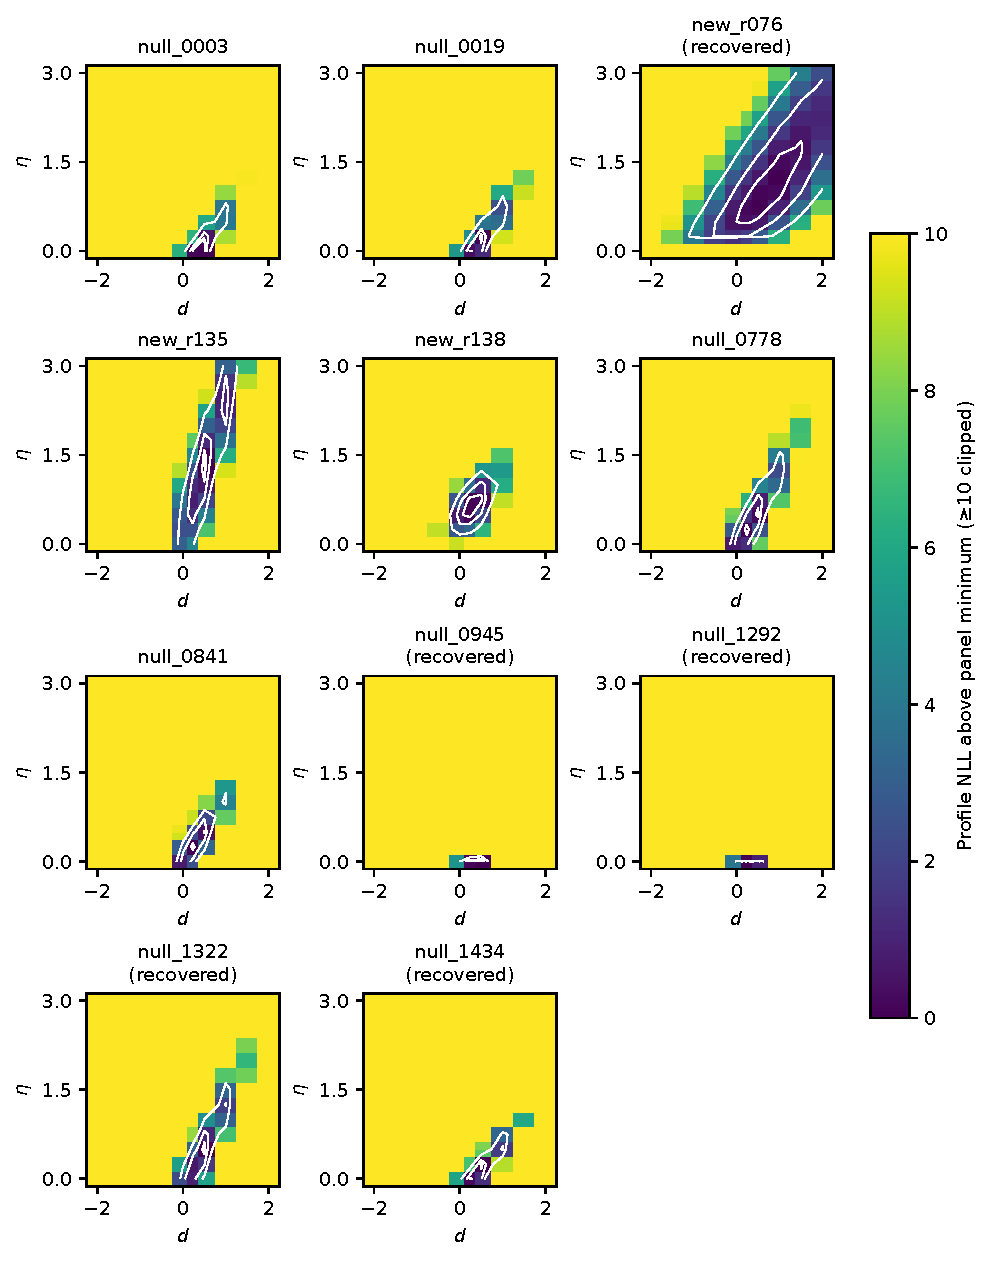
\includegraphics[width=\linewidth,height=.80\textheight,keepaspectratio]{s01_all11_profile_meshes.pdf}
\caption{Completed profile mesh cohort, with recovered panels marked. Each panel subtracts its own grid minimum; colour saturation is labelled. Completing profiles does not complete the historical Hessian diagnostics or establish a global optimum.}
\end{figure}
\begin{figure}[p]
\centering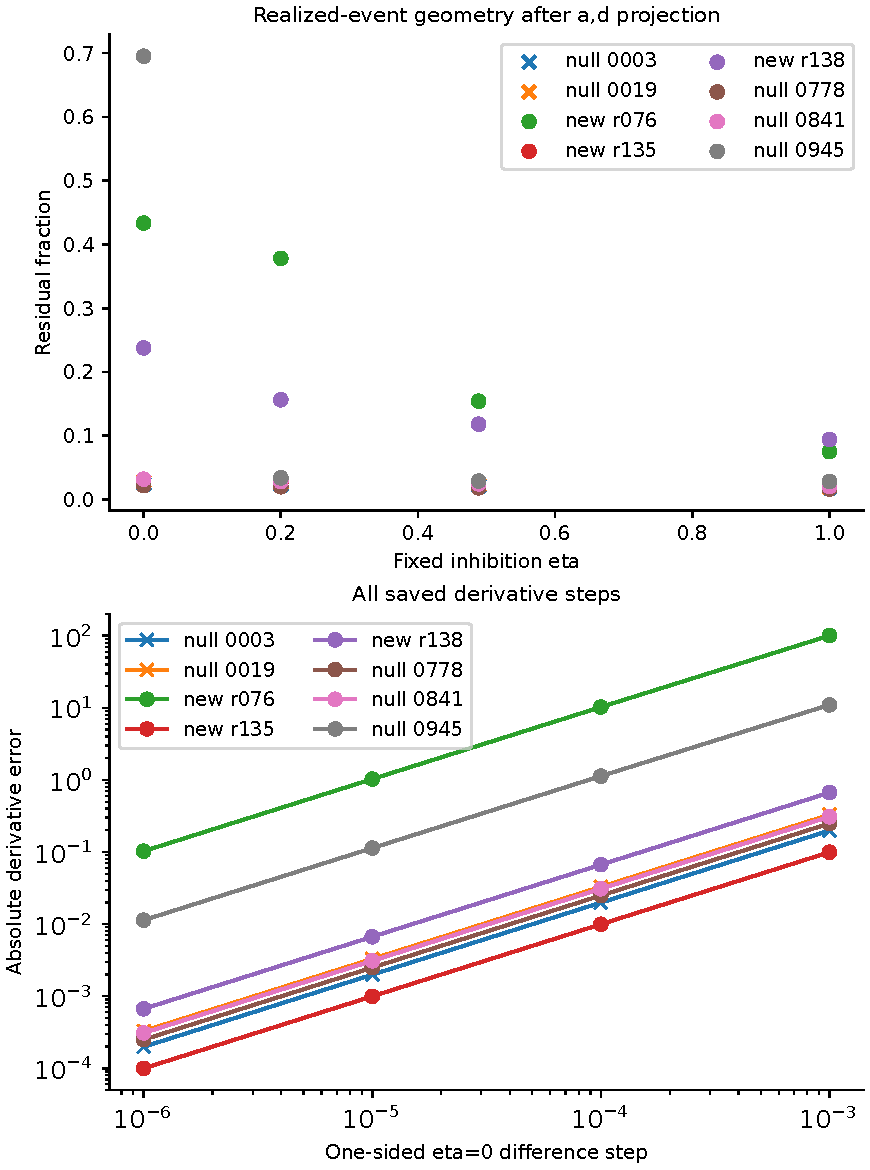
\includegraphics[width=\linewidth,height=.80\textheight,keepaspectratio]{a1_geometry_and_derivative_steps.pdf}
\caption{Realized-event overlap and all saved $\eta=0$ derivative steps.
Positive absolute errors use a log display; exact zeros, if any, are listed
separately without floors, clipping or imputation. Selected old witnesses
remain distinct. Neither panel establishes a causal mechanism.}
\end{figure}

\section{Calibration and uncertainty contract}
Let $R$ be the planned reference count, $K$ the controlled reference indices,
$U=R-|K|$, and $B_q=\sum_{r\in K}\mathbf 1\{T_r\geq T_q\}$ for a controlled
query statistic. The add-one rank interval is
\[
 p_q\in\left[\frac{1+B_q}{R+1},\frac{1+B_q+U}{R+1}\right].
\]
Ties use $\geq$. An uncontrolled query remains unknown. An upper endpoint
at most $\alpha$ gives a definite rejection; a lower endpoint above $\alpha$
gives a definite non-rejection; otherwise the decision remains unknown.
For $N$ planned queries, $k$ definite rejections and $u$ unknowns give
accounting bounds $[k/N,(k+u)/N]$, not sampling confidence intervals.

For the paired nuisance interaction,
\[
 D_i=I_i^{00}-I_i^{10}-I_i^{01}+I_i^{11},\qquad
 \overline D=N^{-1}\sum_iD_i,\qquad
 \operatorname{MCSE}=\sqrt{\frac{\sum_i(D_i-\overline D)^2}{N(N-1)}} .
\]
The declared point summary requires all planned paired rows resolved and
$N\geq2$; it is conditional on the fixed reference bank, not a survivor-only
estimate or reference-bank uncertainty measure.

The executed method used 2,000 shared-reference and paired-query resamples
as a separately gated descriptive sensitivity analysis, not automatic
confirmatory, simultaneous or unconditional coverage. Historical independence
is source-reported, and adaptive pilot/cost-query reuse remains relevant.
Both production jobs ended before final calibration. Independent review
reconstructed base decisions, replayed all 2,000 shared-reference plans and
checked all 80 chunk hashes. It independently recalculated eight declared
query-replicate witnesses.
A separate audit checked all 120 saved endpoint quantiles. This does not mean
every resampled query statistic was independently recalculated.

% Values retained from the independently audited saved-output checkpoint.
\section{Historical bounded checkpoint}
The historical checkpoint inventory retained 2,149 histories: 999 references, 1,000 null
queries and 150 alternative queries. Of 8,596 planned method outcomes,
7,068 have controlled statistics and 1,528 remain unknown. There are 1,752
histories with all four controlled, 18 partial, three with exceptions and
376 never attempted. One of the partial claimed histories was interrupted with
an uncontrolled final method. Registration is not complete computation.
The two production phases produced 1,639 new terminal records and reused
133 immutable carried records; the claim count was 1,640.

At $\alpha=0.05$, the historical checkpoint accounting was:
\begin{center}
\captionof*{table}{Historical incomplete F-continuation decisions and planned-denominator rejection bounds.}
\begin{tabular}{llrrrr}\toprule
Queries & Cell & Reject & Non-reject & Unknown & Rejection bounds\\\midrule
Null ($N=1000$)&$I_{00}$&30&593&377&$[0.030,0.407]$\\
&$I_{10}$&35&588&377&$[0.035,0.412]$\\
&$I_{01}$&31&586&383&$[0.031,0.414]$\\
&$I_{11}$&31&589&380&$[0.031,0.411]$\\\midrule
Alternative ($N=150$)&$I_{00}$&150&0&0&$[1,1]$\\
&$I_{10}$&122&28&0&$[0.8133,0.8133]$\\
&$I_{01}$&150&0&0&$[1,1]$\\
&$I_{11}$&65&82&3&$[0.4333,0.4533]$\\\bottomrule
\end{tabular}
\end{center}
The finite fitting recipe reported here gives 122 rejections out of 150
for $I_{10}$ and 65 rejections, 82 non-rejections and three unknown decisions
for $I_{11}$. These are distinct from the paper's historical counts of
123/150 and 68/150, respectively. A separate source-reported metadata check
matched historical and continuation input identities and case roles; this
compact packet does not reproduce it. No paired historical/continuation
outcome comparison is reported; the counts should not be combined or
interpreted as a paired change in detection.

These are bounds over all planned queries, not confidence intervals or
estimates conditional on successful fitting. Controlled reference counts
are 998, 998, 992 and 997 in cell order; controlled null-query counts are
623, 623, 619 and 620; alternative counts are 150, 150, 150 and 148.
Thus a controlled query can still have an unresolved decision because
reference uncertainty straddles the threshold. Null missingness depends
on history cost, traversal and deadlines; the broad bounds do not establish
empirical 5\% size.

At that checkpoint, the unresolved fraction was too large to establish a useful empirical Type I error rate near the nominal five percent level. Missingness cannot be treated as random: expensive histories, the traversal order and computational limits affect which results resolve. Neither a successful subset nor that checkpoint's resampling repaired the missing null coverage; the completed recovery later in this chapter does so explicitly.

The nuisance-interaction accounting bounds are $[-0.765,0.752]$ under
the null and $[-0.38,-0.36]$ under the alternative. The required full-pair
point mean and MCSE are unavailable for both roles. No survivor-only point
estimate is substituted. On these 150 saved alternative histories, supplying
level and estimating trend gives 150 definite rejections;
estimating both nuisance coordinates is associated with materially fewer
detections. The signed interaction is a procedure contrast, not a causal
effect or proof of physical inhibition.

\subsection{Completed descriptive resampling}
All 2,000 declared replicates completed, using one shared reference plan
across the four cells and both roles, and separate paired query plans by
role. Lower and upper accounting endpoints are summarized separately with
linear/type-7 quantiles. For the alternative $I_{11}$ cell, the 2.5\%, median
and 97.5\% quantiles of the lower endpoint are $(0.3800,0.4333,0.4667)$
for bank-only resampling and $(0.3400,0.4333,0.5200)$ when paired queries
are also resampled. The corresponding upper-endpoint quantiles are
$(0.4067,0.4533,0.4800)$ and $(0.3600,0.4533,0.5400)$.
These summarize sensitivity of incomplete accounting, not certified coverage.
All 120 endpoint quantiles and counts of every replicate status are retained
in the JSON/CSV tables; individual statuses remain in the saved chunk JSON.
No unresolved replicate is discarded. In the alternative
paired-query mode, 126 replicates have a resolved point interaction and
1,874 remain unresolved. This does not resolve the original full-pair point.

\subsection{Posthoc accounting of the continuation pilot}
This subsection concerns the earlier 25-query pilot of this continuation,
not the paper's separate $\eta$-planning experiment (6/25 versus 11/25).
After inspecting the aggregate calibration, a separate saved-evidence check
fixed the original 25 alternative IDs and compared their unchanged carried
scores under the old and expanded reference banks. This was descriptive
posthoc accounting: no fit, rank plan or history was regenerated.
For $I_{10}$, the original cohort changed from $(6,11,8)$ to $(19,6,0)$
in reject/non-reject/unknown counts. The remaining 125 alternatives gave
$(103,22,0)$ under the same final bank. For $I_{11}$, the original cohort
changed from $(6,17,2)$ to $(8,17,0)$ and the remaining cohort gave
$(57,65,3)$. Both cohorts have all rejections in $I_{00}$ and $I_{01}$.
The same 25 fitted scores yield different decisions under the new reference
calibration. This comparison does not isolate bank size from reference
composition, rank resolution or missingness. Neither
this comparison nor the additional query cohort establishes population
causality, independent validation or nominal test size.

\begin{figure}[htbp]
\centering
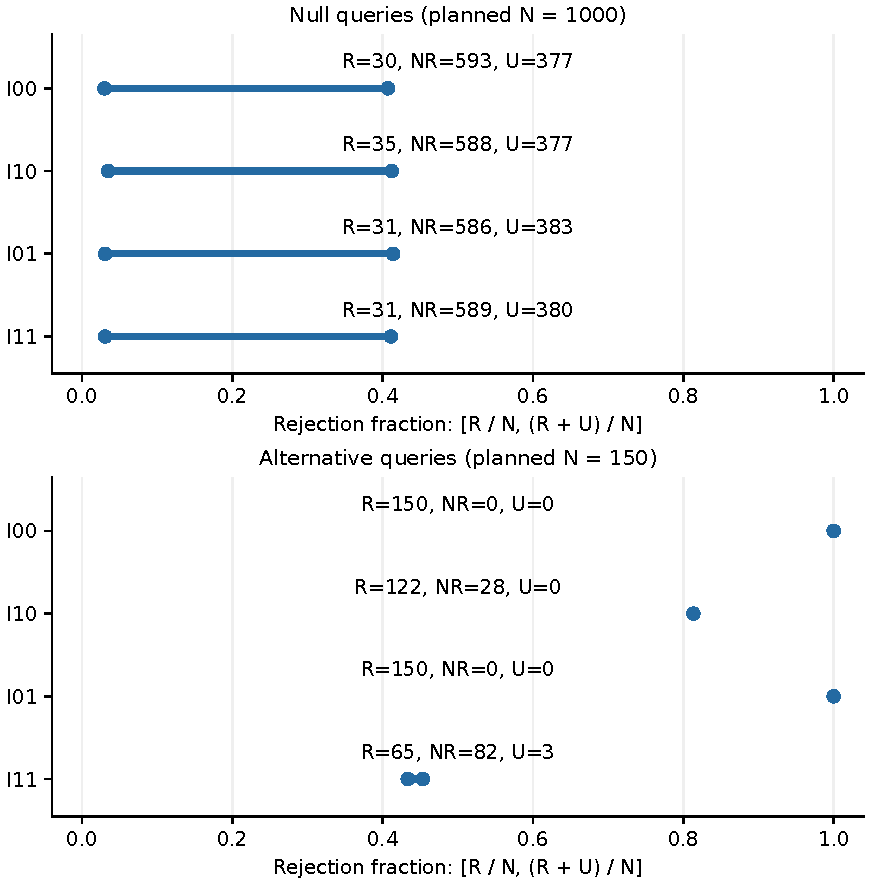
\includegraphics[width=\textwidth]{a1_planned_denominator_bounds.pdf}
\caption*{Historical incomplete calibration on the full planned denominators.
Segments span definite rejection through rejection plus unresolved outcomes;
they are accounting bounds, not confidence intervals. Counts distinguish
definite rejection (R), nonrejection (NR) and unresolved outcomes (U);
reference-bank counts remain in the accompanying text.}
\end{figure}

\begin{figure}[htbp]\centering
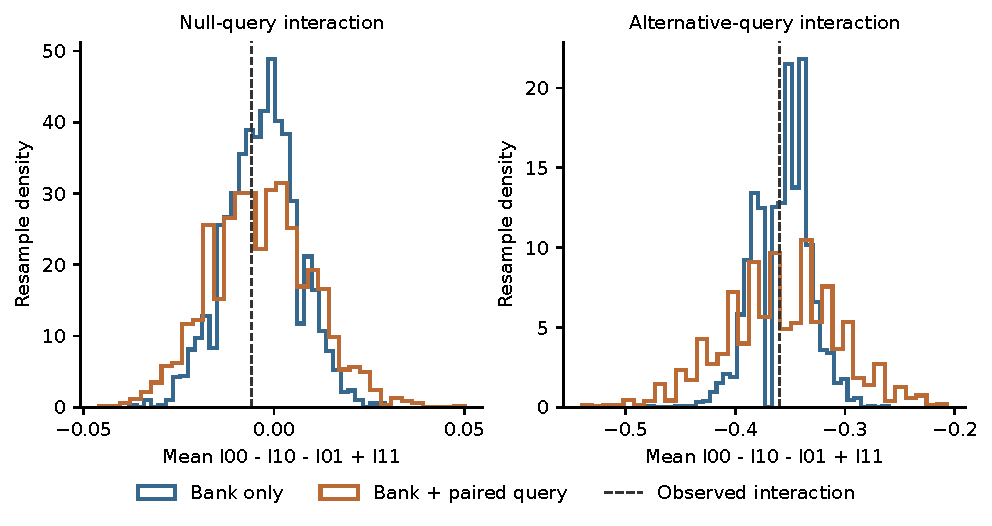
\includegraphics[width=\textwidth]{s01_saved_bootstrap_interactions.pdf}
\caption{The saved 2,000 resampled interaction means for each role and mode.
No additional fit or resampling was performed to draw this figure.}
\end{figure}

\subsection{Decision at the historical checkpoint}
The earlier continuation stopped incomplete and called for a cheaper, numerically validated recovery. The completed missing-only recovery below now supplies resolved counts; it preserves old failures as history and recalculates the rank decisions against the repaired reference bank.

\section{Availability and bounded interpretation}
The 2,149 reused bank byte/clock identities were reverified; the historical
RNG and generating process were not replayed at that checkpoint. The original
source-only delivery omitted the NPZ bank; the recovered-input edition now
supplies its exact histories and role, seed and clock mapping under
\path{reproduction/synthetic/}. Some original F restricted-fit states remain
missing and are not replaced by unrelated earlier fit records.
The accompanying saved summary, accounting tables and figures document the
reported numerical checkpoint; they do not replace the raw-history replay.
The saved \texttt{F\_RESULT\_TABLES.json} records an input
\texttt{summary.json} SHA-256 beginning \texttt{456a3c1f}, whereas
the bundled summary has SHA-256 beginning \texttt{32115580}.
The matrix counts and all displayed endpoint quantiles agree under
saved-value reconciliation; that agreement does not establish byte-identical
input provenance.

Conditional overlap, solver flags and controlled calibration outcomes must be
interpreted together with failures and missing tails. They do not identify
physical inhibition or justify an automatic cache change, retry, new bank,
broader search or next cycle. The separately authorized recovery below addresses that proposal; it retains the predictive and causal interpretation limits.

\subsection{Historical endpoint sensitivity and unresolved interactions}
All endpoint quantiles remain in Appendix~\ref{app:f-endpoints}, Table~\ref{tab:f-all-endpoints}. The repeated point-interaction statuses reduce to the four rows below. The 2,000 resamples per role and mode produced accounting-bound endpoints; an unresolved point interaction does not mean that its endpoint calculation failed. Repeating a status across ten endpoint rows does not create ten new resampling cohorts.
\begin{center}
\begin{tabular}{llrr}\toprule
Role & Resampling & Resolved & Unknown\\\midrule
Null & Bank only & 0 & 2000\\
Null & Bank and paired query & 0 & 2000\\
Alternative & Bank only & 0 & 2000\\
Alternative & Bank and paired query & 126 & 1874\\\bottomrule
\end{tabular}
\end{center}
These are descriptive sensitivity calculations, not confidence limits. Even a resolved resampled point does not resolve the original full-pair statistic or establish null calibration.

% Source: M01/S01_SUMMARY.json SHA256 b04416906237b7dfbaf8af5ef8f08b7e9147d10155e495bfcc9a694a5bb691a8.
% Acceptance: scientific_stage2_resume_20261031T205913Z/integration/S01_ACCEPTANCE.json.
% Figures and complete input bindings: temporal/integration/source_bindings.json.
\section{Completed F-continuation recovery}
The earlier incomplete continuation is a historical checkpoint, rather than
the final coverage statement. The authorized Stage~2 recovery filled only
missing statistics: 11 reference histories, 384 null-query histories and two
alternative-query histories, comprising 397 histories and 1,528 procedure
cells. The earlier shorthand of 383 null and three alternative histories is
superseded by this bound input map. All 7,068 originally controlled cells
were preserved. The final bank contains 999 reference statistics, 1,000 null
queries and 150 alternative queries for each of $I_{00},I_{10},I_{01},I_{11}$,
with no unresolved cells. Calibration uses the same add-one rank rule,
including ties through reference statistics greater than or equal to the
query statistic.

\begin{table}[htbp]\centering
\caption{Completed F-continuation rejection counts. All planned queries are
resolved; these proportions replace the historical missingness bounds as
the current numerical checkpoint.}\label{tab:f-stage2-completed}\label{tab:f-continuation}
\begin{tabular}{lrrrr}\toprule
Queries & $I_{00}$ & $I_{10}$ & $I_{01}$ & $I_{11}$\\\midrule
Null ($N=1{,}000$) & 49 (0.049) & 47 (0.047) & 52 (0.052) & 44 (0.044)\\
Alternative ($N=150$) & 150 (1.000) & 122 (0.8133) & 150 (1.000) & 68 (0.4533)\\\bottomrule
\end{tabular}\end{table}

\begin{table}[htbp]\centering
\caption{Completed recovery coverage. Query counts apply to each of the four procedures; repaired and preserved counts refer to procedure cells.}\label{tab:f-recovery-coverage}
\begin{tabular}{lr}\toprule
Quantity & Completed count\\\midrule
Reference histories per procedure & 999\\
Null queries per procedure & 1,000\\
Alternative queries per procedure & 150\\
Preserved procedure cells & 7,068\\
Repaired missing procedure cells & 1,528\\
Profile meshes & 11 of 11\\\bottomrule
\end{tabular}\end{table}

The completed paired interaction
$\overline D=\overline{I^{00}-I^{10}-I^{01}+I^{11}}$ is $-0.006$ under
the null queries (query-unit Monte Carlo standard error $0.00949$), and
$-0.360$ under the alternatives (standard error $0.04564$).
The 2,000 saved resamples in each role and resampling mode are all resolved.
\begin{table}[htbp]\centering
\caption{Completed paired nuisance-interaction means and query-unit Monte Carlo standard errors.}\label{tab:f-completed-interaction}
\begin{tabular}{lrr}\toprule
Queries & Mean $\overline D$ & Monte Carlo SE\\\midrule
Null ($N=1{,}000$) & $-0.006$ & $0.00949$\\
Alternative ($N=150$) & $-0.360$ & $0.04564$\\\bottomrule
\end{tabular}\end{table}
Their descriptive 2.5th, 50th and 97.5th percentiles appear in Table~\ref{tab:f-completed-bootstrap}.

% Completed Stage 2 bootstrap table; historical endpoints retained separately.
\begin{table}[htbp]\centering
\caption{Completed paired-interaction bootstrap summaries. All 2,000 replicates per row are resolved; quantiles are descriptive resampling summaries.}\label{tab:f-completed-bootstrap}
\begin{tabular}{llrrr}\toprule
Queries & Resampling & 2.5th & 50th & 97.5th\\\midrule
Null & Bank only & $-0.022$ & $-0.003$ & $0.015$\\
Null & Bank and paired query & $-0.029$ & $-0.004$ & $0.023$\\
Alternative & Bank only & $-0.4067$ & $-0.3533$ & $-0.3067$\\
Alternative & Bank and paired query & $-0.4667$ & $-0.3600$ & $-0.2533$\\\bottomrule
\end{tabular}\end{table}


These are reference-bank and paired-query resampling sensitivity summaries,
not certified confidence coverage or an independent population calibration.
The null rates are observed simulation frequencies, not proof of nominal
size for every generating law.

\begin{figure}[htbp]\centering
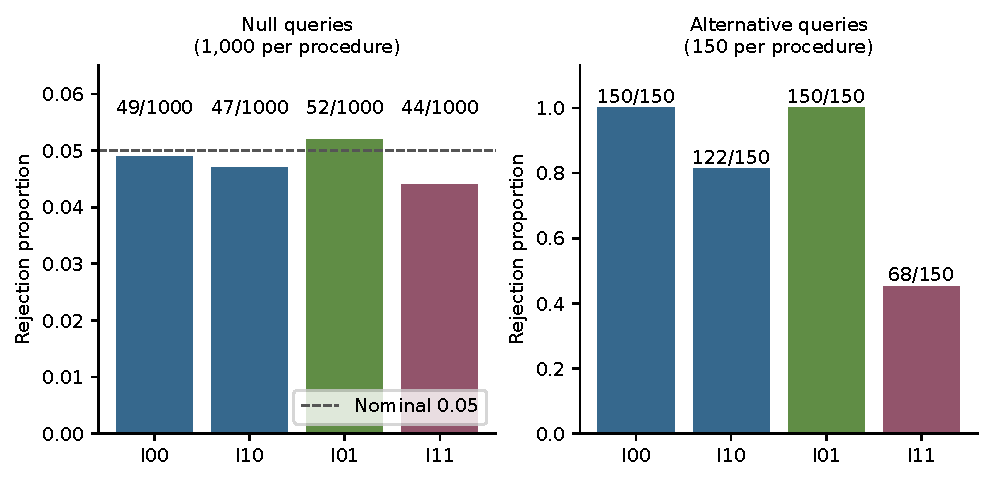
\includegraphics[width=\textwidth]{s01_completed_rejections.pdf}
\caption{Completed planned-denominator F-continuation rejection proportions.
No unresolved outcomes are imputed. The dashed line denotes nominal 0.05.}
\end{figure}



The reference-bank calibration remains an oracle calibration for the
specified synthetic law. It is not a nested fitted-null plug-in calibration:
the proposed 23,760-fit nested bootstrap was excluded by the authorized
scope. Recovery combines original controlled results with an eight-start
compiled procedure only for missing cells, and therefore does not claim
uniform reoptimization of every bank member. Validation comprises 20
resolved-history compatibility controls, independent kernel fixtures and a
three-history raw saved-point pilot, together with complete saved custody
and aggregate arithmetic checks. It does not claim independent raw replay
of every fit or mesh. The finite 195-mode approximation and predictable
pre-event clock convention remain those of the preserved implementation.


\part{Temporal, Mark-History, and Orthogonalized Extensions in New Zealand}
\chapter{Reconstructed New Zealand Baseline and Temporal Diagnostic}
\label{ch:observed}\label{chap:observed}

\section{Scope and provenance of the archived catalogue}

The three test windows contain 203, 155 and 254 events, totalling 612. These same targets are inspected again in the mark-history, productivity, orthogonalization, temporal-kernel and spatial studies of Chapters~\ref{ch:temporal-extensions} and~\ref{ch:nz-spatial}. Later choices were informed by earlier results. Training-only fitting within a frozen stage therefore coexists with sequential adaptive reuse of the evaluation archive; the programme does not provide independent confirmatory holdouts \citep{Dwork2015}.

\paragraph{Execution provenance.}
The recovered-input edition reran the frozen diagnostic fitting recipe from the exact reconstructed catalogue; Section~\ref{sec:autonomous-nz-comparison} reports a separately executed autonomous fit. Earlier restriction calibrations below retain their original records and were not recomputed during this edition.

The empirical analysis begins with an archived catalogue rather than with the unavailable inputs to the original manuscript. The primary archive is a GeoNet WFS snapshot downloaded on 15 October 2026. Events were selected with magnitude \(M\geq 5\) and depth no greater than \(40\)~km, within latitude \([-48.5,-33.5]\) and longitude \([165,180]\). The depth sentinel value \(-9\) was excluded, while other negative depths were retained. The resulting file contains 913 selected events in a 24,394-day observation window, from 1960-01-01 inclusive to 2026-10-15 exclusive. The event count is recorded, together with the filter definition and catalogue metadata, in the archived research report and processed metadata (\hyperlink{S25}{archival \texttt{S25} (recovered archive)}; \href{https://github.com/Drefetr/An_Evaluation_of_Earthquake_Models/blob/61aa599cd023f2441a6a0c6af9aa4b6fe9eda3e5/provenance/catalogue_snapshot_metadata.json}{public metadata extract} (\texttt{S24})).

The reappearance of the number 913 does not establish identity with the event list analysed in the original work. The original frozen data, source configuration, and executable code are absent, so neither event identity nor processing history can be recovered. A second archived FDSN interface from the same provider returned 914 selections, consisting of 913 events common to the primary snapshot and the additional event 2025p672513. These are interface selections from one national provider, not independent physical catalogues. The interfaces share the same provider and much of their processing history; agreement between them cannot serve as independent validation of completeness or magnitude accuracy.

This distinction governs the interpretation of every later comparison. The reconstruction is an independent analysis applied to a documented archive snapshot, not a numerical replay of the historical analysis. The fitted catalogue slope for a continuous excess-exponential magnitude model is \(2.849401764894274\). For comparison with the earlier manuscript's half-bin convention, define
\[
 \widehat\beta_{\mathrm{adj}}
 =\frac{1}{\overline{M-M_0}+0.05},\qquad M_0=5.
\]
Applied to the archived selection, this gives \(2.494071218330174\), consistent in rounded form with the reported value near \(2.494\). This reconciles an estimator convention; mixed precision and native magnitude scales do not establish a common half-bin adjustment as a generally validated correction for this catalogue. The primary continuous estimate, raw magnitudes, productivity normalization and fitted-law records remain unchanged. It does not demonstrate that the historical event sample or likelihood calculation has been reproduced. Completeness above a time-varying threshold, the relation between native magnitude scales, missing parents of smaller or deeper events, activity before 1960, and the adequacy of national pooling therefore remain explicit assumptions (\hyperlink{S27}{archival \texttt{S27} (recovered archive)}).


\begin{figure}[tbp]
\centering
\includegraphics[width=\linewidth]{catalogue.pdf}
\caption{Descriptive summaries of the 913-event archived selection: annual counts, magnitudes and native magnitude labels. The final calendar year is partial. These plots describe this selection and do not establish catalogue completeness or homogeneous observation through time.}
\label{fig:catalogue}
\end{figure}

\section{A restricted diagnostic intensity}

The observed comparison uses the temporal diagnostic defined in the experimental design:
\begin{equation}
 \lambda_\eta(t)=B(t)e^{-\eta G_s(t)}+nH_e(t),\qquad
 B(t)=e^{a+d(2t/T_0-1)},\quad \eta\geq0.
 \label{eq:observed-diagnostic}
\end{equation}
Here the subscript \(s\) denotes stress memory and \(e\) denotes excitation. Neither denotes a spatial coordinate. Both features depend only on strictly earlier events. The implemented Mittag--Leffler (ML) kernels are finite positive spectral mixtures. A shared-memory recipe supplies the same kernel parameters to the stress and triggering features, although those features enter different parts of the intensity. The background is specified independently of the stress history. Thus this family diagnoses a restricted form of inhibition; it does not reproduce the original physical loading construction.

The five observed candidate families were constant Poisson, loglinear Poisson, Omori triggering, ML triggering, and ML triggering with shared inhibition. The principal contrasts compare the last three families. Model labels use ``ML'' for Mittag--Leffler. The native local-magnitude label in Figure~\ref{fig:catalogue} is displayed as \(M_{\mathrm L}\); the original archive label is retained in the data. All five families and their search rules are recorded in \href{https://github.com/Drefetr/An_Evaluation_of_Earthquake_Models/blob/61aa599cd023f2441a6a0c6af9aa4b6fe9eda3e5/engine/iteration_27/configs/observed_frozen.json}{public search protocol (operational adaptation)} (\texttt{S18}).

The temporal Omori comparator uses the normalized triggering density
\[
 h_{\mathrm O}(u;c,p)=\frac{p-1}{c}\left(1+\frac{u}{c}\right)^{-p}
 =(p-1)c^{p-1}(u+c)^{-p},
 \qquad u\geq0,\quad c>0,\quad p>1.
\]
The lag \(u\) is measured in days. Its integral on $[0,\infty)$ is one. The scale $c$ is measured in days and
is stored as \texttt{KernelSpec.tau}; the triggering multiplier $n$ remains
separate. This specifies the temporal comparator used here, not a complete
space--time ETAS construction.

The split is chronological. The absolute trend coordinate is \(x=2t/T_0-1\), where \(T_0=24394\) days. Candidate fits use the first \(0.50\), \(0.65\), and \(0.80\) fractions of the archive horizon as training prefixes, comprising 301, 504, and 659 events. Tests use the following disjoint intervals \(0.50\)--\(0.65\), \(0.65\)--\(0.80\), and \(0.80\)--\(1.00\), containing 203, 155, and 254 events and 612 test events in total. These intervals correspond approximately to 1993--2003, 2003--2013, and 2013--2026, but the fractions and archive day indices are the operative definitions.

All retained history before each origin, including earlier test history, is available to the candidate intensity. Each fit uses only its training prefix. The exponential mark-rate estimate is obtained from training marks alone and is common across candidate families; it is a plug-in estimate rather than a joint marked-intensity maximum-likelihood estimate. The reported score is the full marked-event score: the sum of event log intensities and log mark densities minus the integrated intensity over quiet exposure, with the final censor handled explicitly in the declared protocol. The uninhibited fit is retained as an exact eligible point in the inhibited search, so nonnegative training gain is partly built into candidate selection. This fact limits any inference from training improvement alone. The stored training gains for the shared diagnostic are \(2.731009\), \(0.302486\), and \(0.143866\), but those numbers are not treated as evidence of predictive success.

\subsection{Saved parameters at the predictive origins}\label{sec:saved-fits}
Table~\ref{tab:saved-predictive-parameters} displays the saved selected records for the three triggering families at the three predictive origins, not new fits. The \href{https://github.com/Drefetr/An_Evaluation_of_Earthquake_Models/blob/61aa599cd023f2441a6a0c6af9aa4b6fe9eda3e5/paper/supplements/predictive_parameters.json}{selected-parameter companion}
% Exact companion path: supplements/predictive_parameters.json
 retains all fifteen records for the five families, full precision, source hashes and field pointers. The constant Poisson model fixes \(d=n=\eta=0\); loglinear Poisson fixes \(n=\eta=0\). The table's two uninhibited triggering families fix \(\eta=0\).

\begin{table}[htbp]
\centering\small
\setlength{\tabcolsep}{4pt}
\caption{Saved selected parameters at three predictive origins. The background is \(\exp(a+dz(t)-\eta G_s(t))\) per day, with \(z(t)=2t/24394-1\). Values are rounded for display; zeros in the uninhibited families are fixed.}
\label{tab:saved-predictive-parameters}
\begin{tabular}{llrrrr}
\toprule Origin & Family & \(a\) & \(d\) & \(n\) & \(\eta\) \\ \midrule
50\% & Omori & $-4.712517$ & $-0.457071$ & 0.685640 & 0.000000 \\
50\% & Mittag--Leffler & $-4.458572$ & $-0.252150$ & 0.455824 & 0.000000 \\
50\% & Shared inhibition & $-2.196743$ & 1.789757 & 0.481700 & 1.646714 \\
65\% & Omori & $-4.291554$ & 0.048036 & 0.570076 & 0.000000 \\
65\% & Mittag--Leffler & $-4.188810$ & 0.147441 & 0.497996 & 0.000000 \\
65\% & Shared inhibition & $-3.841844$ & 0.492682 & 0.503490 & 0.211710 \\
80\% & Omori & $-4.394252$ & $-0.196162$ & 0.561216 & 0.000000 \\
80\% & Mittag--Leffler & $-4.282575$ & $-0.056651$ & 0.470292 & 0.000000 \\
80\% & Shared inhibition & $-4.103408$ & 0.127638 & 0.473071 & 0.105254 \\
\bottomrule
\end{tabular}
\par\medskip
\begin{tabular}{lrrrr}
\toprule Origin & \(\beta_{\rm train}\) & \(r\) & Omori \(c\) (days) & Omori \(p\) \\ \midrule
50\% & 3.101622 & 0.4 & 0.012995 & 1.113368 \\
65\% & 3.149488 & 0.7 & 0.020798 & 1.198604 \\
80\% & 3.021907 & 0.7 & 0.006972 & 1.155845 \\
\bottomrule
\end{tabular}
\end{table}

All six selected Mittag--Leffler kernels use \(\alpha=0.5\), the lower searched grid endpoint, and \(\tau=1\) day, an interior grid value. The common selected productivity ratio is \(r=0.4\) at the first origin and \(r=0.7\) at the later origins; the former is the lower searched ratio endpoint. The Omori coordinates \(c,p\) were optimized continuously with a retained coarse-grid floor; they are not merely grid winners. These endpoint descriptions are newly checked arithmetic against the frozen search grids. Historical boundary flags, tolerance-based near-boundary classifications and standard errors were not saved. The selected continuous coordinates are strictly inside their recorded bounds under exact comparison. No uncertainty estimates are inferred.

The rates \(\beta_{\rm train}\) are estimated from training marks alone, held common across families, and frozen during each test. Inactive serialization fields are not fitted coordinates: the saved \(p\) field of a Mittag--Leffler kernel and \(\alpha\) field of an Omori kernel have no role in their respective formulas. 

At the three predictive origins, the selected shared-inhibition recipe's
unattenuated deterministic background is approximately \(9.60\), \(1.57\)
and \(1.34\) times that of the corresponding noninhibited Mittag--Leffler
recipe, respectively. The first-origin fit therefore combines a much larger
baseline with stronger depletion. These are descriptive ratios of fitted
components, not total-intensity ratios or a demonstrated causal explanation
of the subsequent predictive loss.

\section{Earlier calibrated restrictions}

The earlier reconstructed analysis tested two restrictions: no feedback and a common rather than separate memory scale. Its observed statistics were \(0.7036472\) and \(0.0829952\), respectively. The completed fitted-law calibration retained \(1{,}999\) null cases per restriction, giving add-one ranks of \(0.365\) and \(0.263\). Neither restriction was rejected by that declared five-percent procedure. These are conditional ranks, not probabilities that the hypotheses are true. In particular, non-rejection does not demonstrate equal physical memories, and the stress kernel's disappearance at zero feedback limits what such a restriction can establish. The calibration authority is \hyperlink{S01}{archival \texttt{S01} (recovered archive)}; its interpretation is summarized in \hyperlink{S27}{archival \texttt{S27} (recovered archive)}.

The later chronological comparison asks a different question: do the declared inhibited recipes predict subsequent observations better than serious triggering alternatives? A negative predictive result need not contradict a non-rejecting in-sample restriction test. Their targets, fitting rules and calibration differ.

\section{Held-out score comparison}

Table~\ref{tab:observed-scores} reports score differences relative to the ML triggering-only benchmark. Negative values favour the benchmark; positive values favour the named alternative.

\begin{table}[!ht]
\centering
\caption{Descriptive held-out marked-process score differences relative to the ML triggering-only benchmark. Tests are disjoint chronological intervals in the declared archive protocol. Values are differences, not log-likelihoods for separate datasets. Confidence intervals are not reported.}
\label{tab:observed-scores}
\small
\setlength{\tabcolsep}{4pt}
\begin{tabular}{lrrrr}
\toprule
Contrast & Test 1 & Test 2 & Test 3 & Total \\
\midrule
Shared inhibition \(-\) ML & \(-16.517557\) & \(-0.075277\) & \(-1.030025\) & \(-17.622859\) \\
Omori triggering-only \(-\) ML & \(+3.106623\) & \(+2.837708\) & \(+6.513790\) & \(+12.458121\) \\
\bottomrule
\end{tabular}
\end{table}

The shared diagnostic loses in all three folds. Its total disadvantage is driven overwhelmingly by the first block: approximately \(93.7\%\) of the total deficit occurs there. The second-block difference is nearly zero, but that is not strong independent evidence of parity because the training histories overlap and later folding choices were inspected during development. The calculations are exploratory and were not designed as confirmatory or as an independent sequence of repeated tests (\hyperlink{S19}{archival \texttt{S19} (recovered archive)}).

The continuous Omori recipe improves on the finite ML kernel grid in every fold. This result cannot be converted into a universal law ranking. The Omori refinement and the finite spectral ML candidate have unequal flexibility, and the contrast therefore favours the declared Omori recipe under its fitting convention. It is not an isolated estimate of the effect of \(\eta\), nor a demonstration that every continuously refined triggering model dominates every grid-based alternative. Residual diagnostics were descriptive, varied over the record, and did not certify any winner as an adequate physical model.


\begin{figure}[tbp]
\centering
\includegraphics[width=\linewidth]{prediction.pdf}
\caption{Chronological test-score contrasts for the declared recipes. The first test block contributes about 93.7\% of the aggregate shared-inhibition disadvantage. Training prefixes overlap and the periods were reused in exploratory development; the three periods are not independent confirmatory tests.}
\label{fig:prediction}
\end{figure}

\begin{samepage}
\paragraph{Executable replay.}
The recovered-input edition reran the unchanged frozen fitting recipe from the exact reconstructed catalogue: every scientific numerical field in the complete optimizer and diagnostic output matched the historical result exactly. Both complete outputs and the executable comparison are supplied in \path{reproduction/observed/}; the replay includes the prescribed starts, failed solver attempts, selected fits and numerical controls.
\end{samepage}

\section{Score accounting and temporal localization}

For a fold, write the score difference as
\begin{equation}
  \Delta\ell
  = \Delta Q+\Delta C,
  \qquad
  \Delta Q=\sum_i\log\frac{\lambda_{\mathrm{sh},i}}{\lambda_{\mathrm{ML},i}},
  \qquad
  \Delta C=\Lambda_{\mathrm{ML}}-\Lambda_{\mathrm{sh}},
  \label{eq:score-accounting}
\end{equation}
For this temporal model $P=Q$, $E=\int\lambda(t)\,dt>0$, and $C=-E$. Thus $\Delta C=E_{\mathrm{ML}}-E_{\mathrm{sh}}$. The historical event-sum symbol $E$ has been replaced here by $\Delta Q$. The event sum uses pre-event intensities at the realized times, and \(\Lambda\) denotes the corresponding integrated intensity. This separates event-term disagreement from realized compensator disagreement. In the first test block,
\[
\Delta Q=-33.715205,\qquad \Delta C=17.197647,\qquad \Delta\ell=-16.517557.
\]
The integrated intensities are \(115.871595\) under the shared diagnostic and \(133.069242\) under the ML benchmark for 203 events. These are not conventional expected counts from a fixed fitted Poisson model: the compensator is evaluated along an updating estimated history. Its realized value is not automatically the future expected count conditional only on information at the test origin. No naive Poisson count probability value is attached to their difference.

Four equal-duration bins within the first test interval sharpen the accounting without allocating events to bins by any counterfactual rule. Each bin uses the complete preceding history and integrates over its own realized path. Approximate calendar labels are displayed only for orientation; the archive-day boundaries define the calculation.

\begin{table}[!ht]
\centering
\caption{Descriptive score accounting within four equal-duration subintervals of the first test block. Each row uses full preceding history and realized integration within that subinterval. Confidence intervals are not reported.}
\label{tab:first-block-accounting}
\small
\setlength{\tabcolsep}{4pt}
\begin{tabular}{lrrr}
\toprule
Approximate interval & \(\Delta Q\) & \(\Delta C\) & \(\Delta\ell\) \\
\midrule
1993-05-24 to 1995-11-24 & \(-2.891244\) & \(2.464270\) & \(-0.426975\) \\
1995-11-24 to 1998-05-27 & \(-16.875378\) & \(7.143815\) & \(-9.731563\) \\
1998-05-27 to 2000-11-27 & \(-8.696131\) & \(4.642115\) & \(-4.054016\) \\
2000-11-27 to 2003-05-31 & \(-5.252451\) & \(2.947447\) & \(-2.305004\) \\
\bottomrule
\end{tabular}
\end{table}

The deficit is localized in time rather than uniformly spread across the first block. The strongest subinterval loss occurs between approximately late 1995 and mid-1998. This localization does not identify an earthquake sequence, a geological province, or a causal mechanism. It records that the aggregate score is sensitive to when an updating history and its compensator disagree (\hyperlink{S20}{archival \texttt{S20} (recovered archive)}).


\begin{figure}[tbp]
\centering
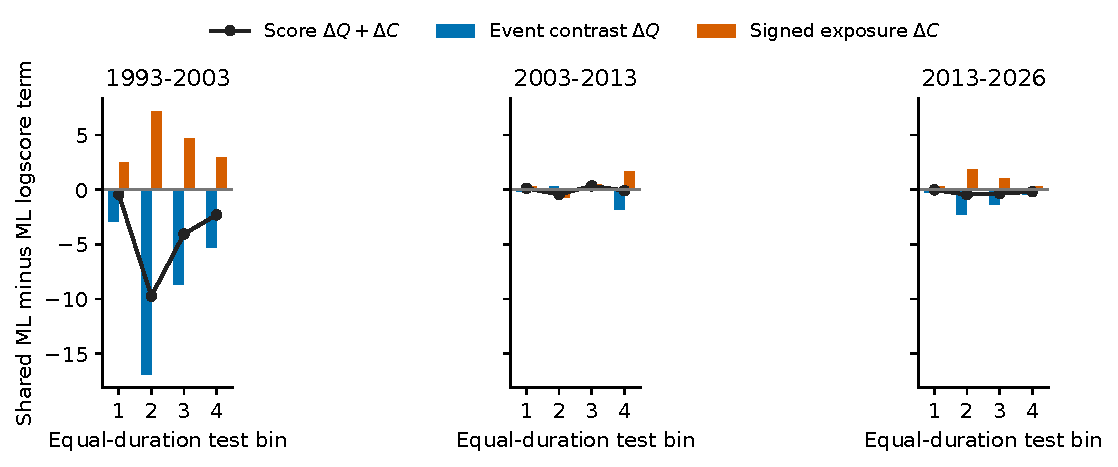
\includegraphics[width=\linewidth]{temporal.pdf}
\caption{Event and compensator contributions in four equal-duration bins in each of the three test periods. The archived figure uses $E$ for the event contrast $\Delta Q$ and $C$ for the compensator contrast $\Delta C$; its $E$ is not the positive exposure $E=\int\lambda(t)\,dt$ used in this volume. Each bin is integrated with complete preceding history. In the first period a favorable compensator contribution partly offsets the negative event term; the full score is $\Delta Q+\Delta C$.}
\label{fig:temporal}
\end{figure}

A spatial and mark audit found that all five occupied coarse cells had negative event-term contributions for the shared-minus-benchmark contrast. The same direction appeared for native ML and \(M_{\mathrm w}\) magnitude conventions and for all declared magnitude and depth groups. The shared specification contains one regional compensator rather than cell-specific or group-specific exposure. Accordingly, these sums are diagnostics of event-term sign under the fitted family, not local likelihoods, local rates, or fractions of the full score. Unequal cell areas, time-location confounding, sparse cells, and reuse of events across overlapping marginal classifications prevent such a local interpretation. Grouping by the current event's mark is descriptive: that mark affects subsequent intensity and does not enter its own pre-event intensity. Native magnitude-label composition changes most strongly in the last block, whereas the dominant loss is in the first, weakening a simple explanation based only on a modern label transition. Completeness and legacy magnitude-scale concerns remain.

\section{Archive sensitivity}

A replacement audit matched all 913 event identifiers and found 241 numerical magnitude differences, the largest absolute difference being \(0.164143665\). Many differences were only in small decimal places. The full history was rescored using alternate matched magnitudes while primary clocks, locations, depths, the fitted \(\beta\), and the recipe definitions were fixed. The additional event in the 914-event interface selection was excluded, and no parameters were refitted or physically converted between magnitude scales.

Under this replacement, the total shared score changed as follows:
\[
 -17.622859365\ \longrightarrow\ -17.617975447,
 \qquad \text{change }+0.004883918.
\]
No fold changed sign. The Omori total changed from \(12.458121\) to \(12.441651\), shown to six decimal places. Thus the tested archive value discrepancy does not explain the recipe failure. Equally, this bounded audit does not eliminate every observational uncertainty in magnitudes, depths, locations, completeness, or event identity.


The observed evidence in this chapter is therefore selective and conditional. The held-out scores are unfavourable to the implemented shared-inhibition recipes, the source-magnitude audit does not reverse that pattern, and the strongest loss is temporally localized. These findings constrain the current diagnostic families. They do not establish the absence of physical shared memory in the Earth system.

The \href{https://github.com/Drefetr/An_Evaluation_of_Earthquake_Models/blob/61aa599cd023f2441a6a0c6af9aa4b6fe9eda3e5/paper/data/prediction.json}{public predictive summary} and the \hyperref[sec:source-supplements]{availability guide} provide public entry points. The exact selected catalogue and complete historical and newly executed fitting outputs are supplied in \path{reproduction/nzca/} and \path{reproduction/observed/}. The command \path{scripts/reproduce_observed.py} rebuilds the fitted results from the catalogue and compares their scientific fields.


\section{Fitting an autonomous finite-mode subfamily}
\label{sec:autonomous-nz-comparison}

This section reports a separately executed fit of the raw constant-background
intensity family already used in Chapter~\ref{ch:temporal-extensions}
(Tables~\ref{tab:A-constant_background} and~\ref{tab:AG-constant_background}).
It makes the mapping to the autonomous theorem explicit; it does not introduce
a distinct intensity family.
Set constant loading $\rho=0$, link $\Psi(X)=\exp(a+X)$, and initial modes
$Z_j(0)=U_j(0)=0$. Retain the diagnostic recipe's fixed finite mixture and mark
scalings. With physical stress release $\eta g_d$ and productivity $n\kappa_d$,
the mode equations give
\[
 \begin{gathered}
 G(t)=\sum_{T_i<t}g_d(Q_i)\Phi(t-T_i),\qquad
 H(t)=\sum_{T_i<t}\kappa_d(Q_i)h(t-T_i),\\
 \lambda(t)=\exp\{a-\eta G(t)\}+nH(t),\quad h=-\Phi'.
 \end{gathered}
\]
Here $g_d(Q)=\exp\{\gamma(Q-1)\}$ and
$\kappa_d(Q)=(1-r)\exp(\beta rQ)$ use the existing fixed diagnostic scalings.
Under the posited independent exponential mark law,
$\mathbb E[\eta g_d]=\eta e^{-\gamma}\beta/(\beta-\gamma)$ when
$\eta>0$ and $\beta>\gamma$, while $\mathbb E[n\kappa_d]=n<1$.
At $\eta=0$ stress release is identically zero. Since $X\leq0$, the link is
bounded and Lipschitz on the reached half-line. These are the relevant
first-moment conditions of Theorem~\ref{thm:finite_mode}; zero initialization
is not a stationary draw.

For general constant loading, event-free equilibrium initialization
$Z_j(0)=\rho/\vartheta_j$ instead gives
\[
 X(t)=\rho\sum_j\frac{w_j}{\vartheta_j}-\eta G(t),\qquad
 a_{\mathrm{eff}}=a+\rho\sum_j\frac{w_j}{\vartheta_j}.
\]
Loading and intercept are therefore confounded; zero loading is a convention,
not an estimate. Equal non-equilibrium initial modes contribute
$X_0\Phi(t)+\rho\int_0^t\Phi(u)\,\dif u$, generally not an affine trend.
Neither convention is stationary event-process initialization.
Section~\ref{sec:finite-stability} quantifies the certificate's practical limits.


Each training prefix fixes the common estimate
$\hat\beta=N_{\mathrm{train}}/\sum Q_i$. The null fits $(a,n)$ at $\eta=0$;
the inhibited arm fits $(a,n,\eta)$ and retains the exact fitted null as a
candidate. Selection uses training likelihood only. All prescribed starts
completed, every returned vector and solver diagnostic is retained, and the
training and held-out quadrature checks and mark-moment gates passed.
Earlier parents and the final event-free tail are included. The frozen
protocol, executable fit and complete outputs are supplied under
\path{experiments/autonomous/} and \path{validation/live_results/}.

The earlier raw constant-background procedure used the conditional-within-bin
training estimate of the magnitude rate. The present estimate changes the
productivity weights as well as the common mark score. The prescribed starts,
solver tolerances, recovery settings and candidate accounting also differ.
Consequently these are different fitted procedures within the same intensity
family, and their score difference is not an isolated effect of changing
$\beta$. The earlier aggregate remains in
Table~\ref{tab:AG-constant_background}; the supplied protocol comparison
records both recipes without replacing either result.


\begin{table}[htbp]
\centering
\small
\begin{tabular}{lrrr}
\toprule
Fold & Null score & Inhibited score & Gain\\
\midrule
Early & -291.5675 & -301.5859 & -10.0184 \\
Middle & -170.2334 & -170.2334 & 0.0000 \\
Late & -523.5999 & -526.5270 & -2.9272 \\
Pooled & --- & --- & -12.9456 \\
\bottomrule
\end{tabular}
\caption{Held-out marked log scores and inhibited-minus-null gains for the
autonomous finite-mode subfamily, in nats. The common mark contribution
cancels from each gain; this is an occurrence-score comparison. The middle
fold selects $\hat\eta=0$: its displayed tie contains only a small
shared-coordinate optimization difference. These contrasts are descriptive;
confidence intervals are not reported.}
\label{tab:autonomous-nz}
\end{table}

The early and late fits select positive inhibition and lose held-out score;
the middle fit selects zero inhibition. The pooled gain is -12.9456 nats.
This exploratory comparison fits the autonomous theorem's model class on
reused chronological observations. Stability implies no predictive advantage,
and the fixed mark and kernel settings preclude full joint nuisance estimation.

\chapter{Magnitude History, Productivity Sensitivity, Exposure Orthogonalization, and Kernel Refinements}
\label{ch:temporal-extensions}\label{chap:temporal-extensions}
The historical observed comparison is retained in Chapter~\ref{ch:observed}.
This chapter consolidates the separately frozen magnitude-history and
productivity studies, followed by exposure orthogonalization, parent-class
temporal scales and continuously tuned Omori triggering. Each comparison uses
its own matched reference. The same historical targets recur across sensitivity
settings; they do not become independent replications.

This reuse is sequential and adaptive at programme level: inspected results helped motivate later model families, parameter domains and reporting contrasts. A protocol frozen before one stage constrains that stage's execution but does not restore an unused holdout after earlier inspection. The resulting scores are exploratory comparisons on a shared archive, subject to the adaptive-data-analysis distinction discussed by \citet{Dwork2015}.

For the temporal models, $P=Q$, timing is $Q+C$, and the joint marked score is
$P+C+M$, with $E>0$ integrated exposure and $C=-E$. Reported differences are
candidate minus the named reference. The source reports' event field (sometimes
called $E$ historically) is displayed here as $\Delta Q$; their compensator
contrast is $\Delta C$. The magnitude excess $q=M_{\rm magnitude}-5$ must not
be confused with the score component $M$. The class cutoff denoted $c$ in the
class-history equations is $c_{\rm class}=0.5$ magnitude units, whereas $c$
in the Omori sections is a temporal scale in days. These are separate local
namespaces. The free-productivity coordinate is continuous on $[0,0.95]$;
the seven-node grid below is a descriptive profile, not its optimization domain.


\section{The earlier magnitude-history misspecification pilot}
\label{sec:magnitude-history-pilot}
The run \path{magnitude_history_20261023T205716Z} precedes the observed
class-history forecast investigation. It asks whether changing magnitude
dependence alters a preserved inhibitory fitting procedure's preference under
a designed, entirely excitatory generating family. It is neither a fitted
comparison of the richer excitatory family nor a forecast experiment.

For magnitude excess $q$ with exponential rate $b$ and bin cutoff $a_{\rm bin}$, let $p_0=1-e^{-b a_{\rm bin}}$ and $p_1=e^{-b a_{\rm bin}}$. The bins are $[0,a_{\rm bin})$ and $[a_{\rm bin},\infty)$. Let
$P_{ij}(h)=(1-h)p_i+h\mathbf1_{i=j}$. With common normalized waiting density
$k$ and no magnitude productivity in the generator,
\[
 \lambda_i(t)=\mu p_i+n_g\sum_{k:t_k<t}P_{iJ_k}(h)k(t-t_k),\qquad
 \Lambda(t)=\mu+n_g\sum_{k:t_k<t}k(t-t_k).
\]
Generate the untyped timed branching forest first. Since the columns of $P$
sum to one and $Pp=p$, assigning immigrant classes from $p$ and child classes
from the parent's column preserves each node's marginal class law by induction.
Fixed-window censoring and chronological ordering depend only on the untyped
forest, so this remains an exact finite-window statement conditional on the
entire timed forest and its event count. Mixing the exponential law restricted
to each bin recovers exactly the same exponential one-event magnitude law.
At $h=0$ the marks are iid; positive $h$ changes labelled-history dependence
without changing total timing or one-event marginals. Class counts at positive
$h$ need not be multinomial, and conditioning on label-selected subsets does
not preserve this argument. In particular, with class histories $S_i$ and
$S=\sum_iS_i$,
\[
 \frac{\lambda_i}{\Lambda}
 =p_i+\frac{n_gh}{\Lambda}(S_i-p_iS).
\]
Each absolute class intensity is nonnegative and receives nonnegative event
increments even though its conditional class probability can decrease.

The same timed forest is labelled under all three persistence scenarios using
fixed per-node random inputs and separate time/mark streams. The independent
replicate is the forest, not each scenario catalogue or each event. The old
candidate uses magnitude-productivity exponent $r=0.7$, whereas the generator has no magnitude productivity ($r=0$, or $\gamma=0$ in its parameterization). Its finite-mixture temporal representation also differs from exact Mittag-Leffler generation. The candidate therefore remains misspecified even
at $h=0$; the mismatches are common across scenarios. Supplied-background
settings do not become true generator parameters. Positive nested fit gains
therefore cannot be interpreted as calibrated false-positive rates.

\subsection{Generator settings and fitted statistic}

The generator is a designed two-class MDFHP-form excitatory family with common Mittag-Leffler shape $0.5$ and scale $1/\mathrm{day}$, total immigrant rate $\exp(-4.162108473051707)$, offspring mean $0.5$ and empty prehistory over 24,394 days. Magnitude excess has marginal exponential rate $2.849401764894274$, with bins $[0,0.5)$ and $[0.5,\infty)$. The $\gamma=0$ productivity boundary and unbounded final bin are explicit extensions of the published fitted specification.
Selection was frozen as direct $\mathrm{GLR}>0.001$ and selected $\eta>\text{\texttt{1e-6}}$. No Wilks reference law, calibrated rejection cutoff, power ranking or physical-mechanism interpretation was used.

For scenario $h$ and planned independent skeleton $s$, let $G(s,h)$ be the procedure's resolved direct likelihood-ratio statistic and $\eta(s,h)$ its selected inhibition parameter. The frozen descriptive preference indicator equals $1$ when $G$ exceeds $0.001$ and $\eta$ exceeds $\text{\texttt{1e-6}}$. These thresholds define an operational preference; they are not calibrated significance cutoffs. The primary contrasts compare the preference indicator and continuous statistic at positive $h$ with the matched baseline at $h=0$ on the same skeleton.

Every scenario's planned denominator is retained. Resolved-only frequencies estimate a resolution-conditional descriptive quantity, with its denominator stated. If $k$ cases select inhibition and $u$ cases are unknown out of $N$ planned cases, the all-planned selection frequency is bounded by $[k/N,(k+u)/N]$. These are missing-outcome accounting bounds, not confidence intervals. Continuous-statistic summaries based on resolved cases remain conditional summaries; missing continuous values are not replaced by zero.

The frozen persistence values are $h=0$, $0.5$ and $0.9$. The actual pilot kernel has Mittag-Leffler shape $0.5$ and inverse-time scale $c=1\,\mathrm{day}^{-1}$, corresponding to the time scale $1/c=1$ day. This pilot $c$ is distinct from the Omori time scale used later in this chapter. The independent compiled core supports only shape $0.5$ and $1$; support for another shape is not claimed. Here $b$ is the continuous mark rate and $n_g$ is the generator branching mean. They are distinct from similarly named shape/productivity parameters in the preserved comparison engine.

The frozen primary procedure estimates background level and trend together with the inhibition alternative, while retaining the staged procedure's supplied triggering, stress and mark-rate settings. Its prescribed starts comprise two null fits followed by two alternative starts from the selected null. A secondary supplied-background procedure uses two inhibition starts. The supplied-background label does not mean its nuisance settings are true generating parameters.

This source-bound six-start staged comparison is narrower than the historical full kernel/productivity searches, the separate later nuisance continuation or the observed-catalogue fitting recipe. Results must identify this exact procedure. They cannot be substituted into historical counts, reference banks or claims about the larger searches. Solver starts, explicit $\eta=0$ eligibility, subset floors, failure-only recovery and original numerical controls remain part of the procedure. Local optimization is not a global optimum certificate.

The $h=0$ scenario is the experiment's independence baseline, not an in-model null-size experiment for the old procedure. The generator has $\gamma=0$ magnitude productivity, while the old candidate intensities depend on prior continuous marks through their productivity and stress transforms. Exact Mittag-Leffler generation and the old finite-mixture representation also remain distinct. These mismatches are common to the persistence scenarios; the paired persistence contrast isolates the change in magnitude history within this deliberately specified stress family, without establishing correct specification at $h=0$.

The primary comparison uses the same realized continuous marks and exposure for its excitatory and inhibitory candidates. A common mark-density term can cancel within that paired comparison, but marks still enter subsequent candidate intensities. Dropping a common density term does not justify discarding the marks. No comparison of raw continuous densities with discrete bin masses is made, and no held-out forecast-score claim follows from these fitted-statistic preferences.

\subsection{Pairing, numerical exposure and reproducibility limits}

The plan contains 20 independent untyped skeletons, each labelled under all three persistence scenarios. There are 60 scenario catalogues but 20 independent replicate blocks. Pairing shares the untyped skeleton and fixed per-node random inputs, while each scenario generates its own conditional labels and within-bin magnitudes. One fixed iid mark sequence must not be reused as the observed marks in every scenario.

Separate time and mark pseudorandom streams, their exact implementation, the compiler and runtime are pinned. Equal seeds in another language or standard-library implementation are not asserted to reproduce the same streams. Uncertainty for persistence contrasts resamples skeleton blocks. Resolved-only paired contrasts state the number of paired-resolved skeletons; all-planned bounds additionally retain unknown preference indicators. Pilot intervals are exploratory Monte Carlo summaries, not confirmatory coverage certification.

The synthetic window is fixed independently of the first and last events. The likelihood retains initial quiet exposure, every positive event gap and the final no-event interval. Saved two-part timestamps and positive gaps define ordering, including cases where a lossy binary64 projection ties. The generator reports a precision failure when its declared parent-child wait-error gate is exceeded; it does not redraw a wait, jitter an event or replace a magnitude to force completion. Resource caps and unresolved mandatory solver states stay explicit unknown outcomes.

The computational route combines an independently implemented C++ generator/numerical core, an R interface and the preserved Python comparison machinery with its declared CUDA/FP64 primary route and existing failure-only recovery. It is not a full rewrite of the historical engine. Independent mathematical/spectral-quadrature, saved-clock and waiting-law controls have separate evidence and declared finite scopes.

An additional reference bridge ran the original released ml.m in GNU Octave. A private byte-preserving copy changed only the C++ dispatch switch to select its original language implementation; the copyright notice and original clone were retained. Fixed-input survival and kernel calculations were compared against the new independent core. This is executable original-source validation without MATLAB, not reproduction of the original MATLAB optimizer, all fitted examples or every numerical regime.

The exact author preprint is separately pinned from the version of record. The exact published supplement remains unavailable in this run, the released Japan CSV contains no event rows, and historical banks excluded from the existing public package remain unavailable. Those gaps constrain exact-reproduction claims; they do not authorize reconstructing historical inputs by guesswork. Third-party source copies and raw catalogue material are not covered by a blanket project licence and remain outside a tidy public payload unless their terms are established.

$\gamma=0$ is a boundary/limiting case of the released positive-productivity fitting transform. The unbounded final magnitude bin extends the article's finite upper magnitude support. The accurate model label is a designed MDFHP-form excitatory stress family with matched exponential marginal marks, not an exact recovered author fit or the entire MDFHP family.

No correctly specified richer excitatory model is fitted in this bounded pilot. A changed inhibitory preference would demonstrate a vulnerability or response of the selected old procedure under this generator; it would not establish that an estimated MDFHP practically absorbs the effect in observed data. Conversely, a small or unresolved contrast would be limited to this family, sample budget and fitting procedure; it would not rule out other magnitude-history mechanisms.

There is no fresh null calibration, size-matched power comparison, observed-catalogue evaluation, causal intervention or physical inhibition identification. Pointwise checks cannot establish uniform performance over nuisance parameters. No combined inhibitory MDFHP, general exact-memory stability theorem, exhaustive novelty claim or external-publication conclusion is asserted. Final claims require terminal saved outputs, complete failure accounting and independent review.

\section{Historical pilot results and interpretation}

The validated machinery is feasible, and the full bounded pilot completed: 20 independent timed forests, three magnitude-dependence scenarios, 60 catalogues and 120 resolved method outcomes. No planned outcome is missing.

Under the frozen descriptive rule, the primary fitted-background comparison preferred positive inhibition in 15/20 independent-mark controls, 17/20 moderate-dependence histories and 18/20 strong-dependence histories. However, both primary paired GLR-difference intervals span zero. This pilot does not establish a clear increase in likelihood evidence specifically caused by magnitude history, or explain previous observed-catalogue evidence.

A nested, unpenalized alternative can improve fit under an excitatory generator. The rule below resolves a positive fit preference near numerical tolerance; these frequencies are not calibrated false-positive rates and do not demonstrate failure of any advertised calibrated inhibition test.

\subsection{Complete outcomes}

All 20 cases per scenario resolved, so resolution-conditional and all-planned frequencies coincide here. Wilson intervals describe Monte Carlo selection frequencies under this rule. They do not calibrate the test. Missing-outcome bounds are retained in the machine-readable summary and are not confidence intervals.
{\small
\setlength{\tabcolsep}{3pt}
\begin{longtable}{llrrrrr}
\caption{All six descriptive pilot frequency cells. Wilson endpoints are frequency fractions across independent forests; they do not calibrate the inhibitory test.}\label{tab:pilot-frequency}\\
\toprule
Procedure & $h$ & Selected/planned & Unknown & Wilson lower & Wilson upper & Median GLR\\\midrule
\endfirsthead
\toprule
Procedure & $h$ & Selected/planned & Unknown & Wilson lower & Wilson upper & Median GLR\\\midrule
\endhead
Supplied & 0.0 & 6/20 & 0 & 0.145477 & 0.518973 & 0.000000\\
Supplied & 0.5 & 6/20 & 0 & 0.145477 & 0.518973 & 0.000000\\
Supplied & 0.9 & 4/20 & 0 & 0.080658 & 0.416017 & 0.000000\\
Fitted (primary) & 0.0 & 15/20 & 0 & 0.531299 & 0.888138 & 1.205812\\
Fitted (primary) & 0.5 & 17/20 & 0 & 0.639581 & 0.947631 & 1.053431\\
Fitted (primary) & 0.9 & 18/20 & 0 & 0.698966 & 0.972134 & 1.052331\\
\bottomrule
\end{longtable}
}

\subsection{Paired changes from the independent-mark control}

Each contrast uses all 20 paired forests and the predeclared 20,000-resample skeleton bootstrap, seed 2026102499. These are exploratory percentile summaries, not confirmatory coverage guarantees. A zero or zero-touching interval is not proof of equivalence.

The primary selection frequency rises, but its median GLR does not increase and its paired mean GLR changes are small relative to their uncertainty. The secondary procedure moves in the opposite direction at strong persistence. These observations do not support a simple, procedure-independent claim that stronger magnitude history yields stronger inhibitory evidence.

The post-execution class-manipulation diagnostic is recorded separately in methods/pilot\_input\_diagnostics.json: observed parent-child same-class fractions were approximately 0.6304, 0.8207 and 0.9656, versus design expectations 0.6346, 0.8173 and 0.9635. This is a descriptive implementation diagnostic, not a new primary test; no event-iid uncertainty is asserted.

\noindent The pilot implementation, validation and resources are retained in \hyperref[app:audit09-pilot-implementation]{Appendix~\ref{app:audit09-pilot-implementation}}.
{\small
\setlength{\tabcolsep}{3pt}
\begin{longtable}{llrrrrrr}
\caption{All four paired changes from the independent-mark control. Selection changes are frequency fractions (multiply by 100 for percentage points); endpoints are exploratory paired-forest bootstrap summaries, not confirmatory coverage.}\label{tab:pilot-paired}\\
\toprule
Procedure & $h$ & Selection diff. & Lower & Upper & GLR diff. & Lower & Upper\\\midrule
\endfirsthead
\toprule
Procedure & $h$ & Selection diff. & Lower & Upper & GLR diff. & Lower & Upper\\\midrule
\endhead
Supplied & 0.5 & 0.000000 & 0.000000 & 0.000000 & -0.010306 & -0.039395 & 0.018140\\
Supplied & 0.9 & -0.100000 & -0.250000 & 0.000000 & -0.040430 & -0.073392 & -0.012346\\
Fitted (primary) & 0.5 & 0.100000 & 0.000000 & 0.250000 & -0.162155 & -0.846990 & 0.354902\\
Fitted (primary) & 0.9 & 0.150000 & 0.000000 & 0.300000 & 0.030885 & -1.114732 & 1.029795\\
\bottomrule
\end{longtable}
}

\begin{figure}[tbp]
\centering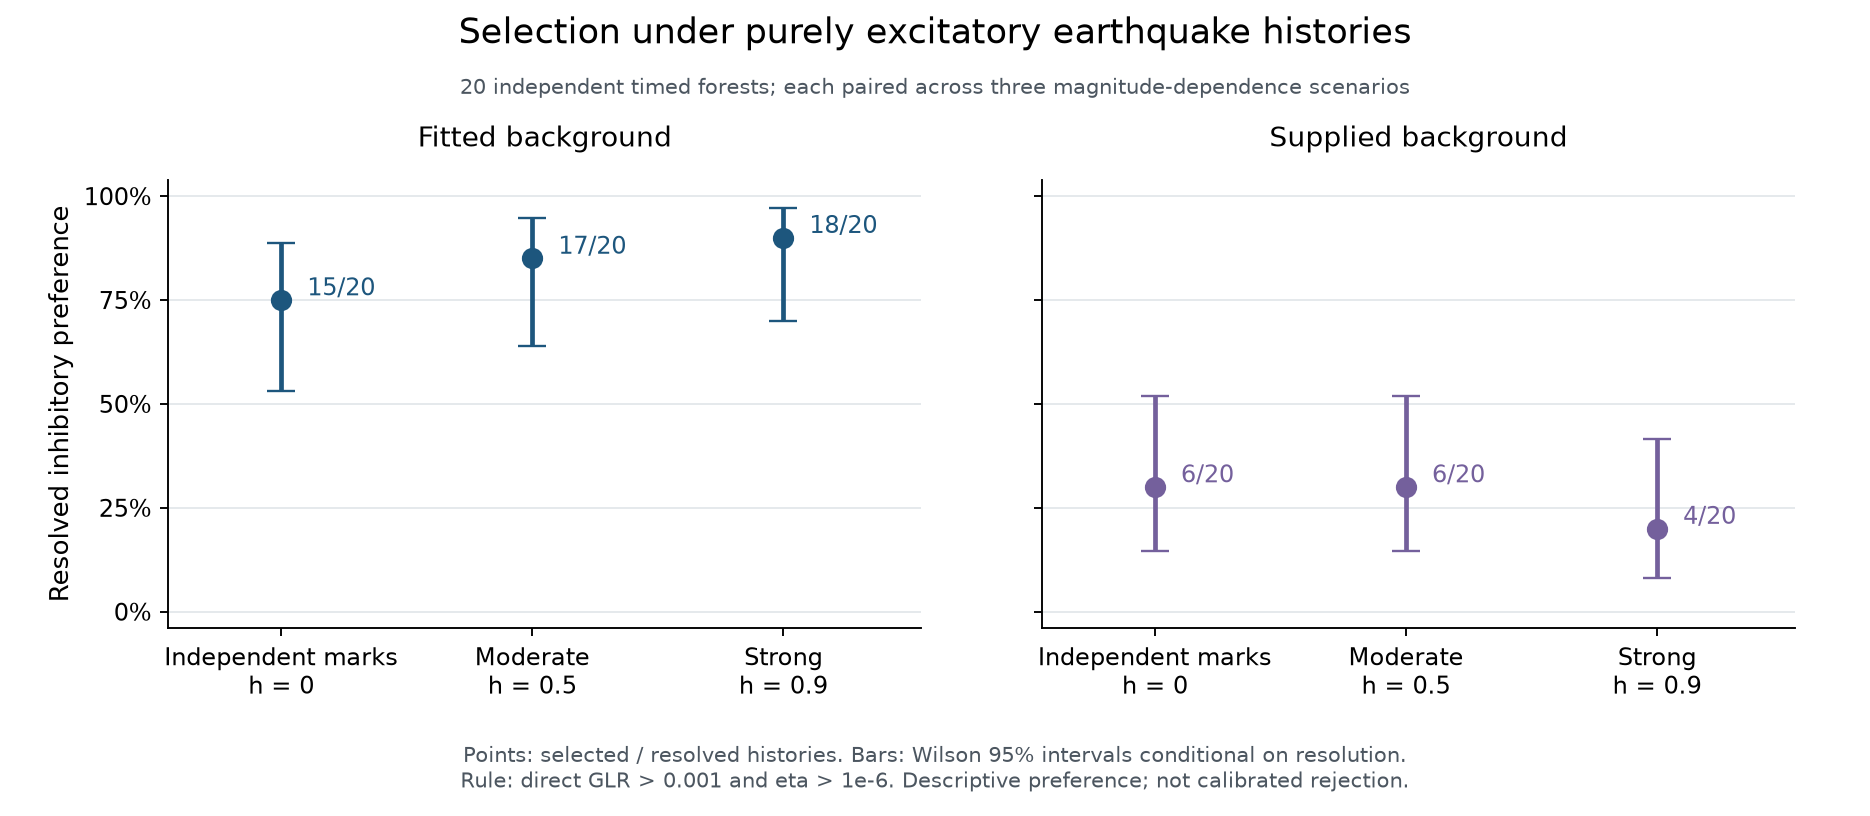
\includegraphics[width=\linewidth]{a2_pilot_selection_final.png}
\caption{Saved final magnitude-history pilot selection frequencies. Forests
are paired across scenarios. These descriptive Monte Carlo intervals do not
calibrate a rejection test or establish a magnitude-history mechanism.}
\label{fig:magnitude-history-pilot}
\end{figure}

\subsection{Interpretation}

The feasibility and bounded descriptive pilot gates pass. The machinery can generate the intended history-dependent marks and apply the selected existing comparison reproducibly. The completed observation is that this narrow procedure can show positive inhibitory fit preference under a purely excitatory designed family, including its independent-mark control.

Whether accounting for magnitude history explains previous observed evidence remains unresolved. No correctly specified richer excitatory model was fitted in this cycle; known-law scoring controls are separate from fitting. There was no fresh null calibration, size-matched power comparison, observed-catalogue evaluation or held-out forecast comparison.

The next scientific stage should first define the claim and fit the competing excitatory family under a reviewed protocol, while separating common productivity misspecification from the history contrast. Any advertised rejection test then needs fresh calibration and independent evaluation banks reproducing nuisance fitting and selection. An observed-data comparison would require matched scoring targets/exposure and separate catalogue/completeness gates. No additional campaign was launched here.

\noindent The pilot reproducibility artifacts are retained in \hyperref[app:audit09-pilot-artifacts]{Appendix~\ref{app:audit09-pilot-artifacts}}.

\noindent The pilot evidence map is retained in \hyperref[app:audit09-pilot-evidence]{Appendix~\ref{app:audit09-pilot-evidence}}.

\section{Purpose and relationship to the earlier releases}
\label{a2:purpose}

The original GitHub research manuscript separates mathematical legitimacy,
identification of an observation law and the predictive value of a fitted
procedure (Chapter~\ref{ch:observed}; Appendix~\ref{app:custody}). Its first addendum examined a separate
background-nuisance continuation whose initial null gap is closed in
Section~\ref{sec:f-continuation} (Appendix~\ref{app:custody}). This second companion adds a different empirical
axis: whether magnitude-class history or a more flexible magnitude-productivity
law improves the declared predictive comparisons. It reports the two completed
follow-ups, their numerical evidence and their stopping decisions, preserving
the earlier scientific records.

The distinction between releases is substantive. The manuscript's observed
reconstruction selected productivity ratios \(r=0.4,0.7,0.7\) at its three
origins. The new matched reference candidates use \(r=0.7\) throughout and a
different, common training-only magnitude-rate estimator
(Table~\ref{a2:recipe}). They are separately specified follow-up experiments,
not replacements for the manuscript's historical score table. Both use the
same hash-pinned GeoNet selection as our observed reconstruction. That archive
identity does not establish identity with the unavailable earlier analysis
discussed in the manuscript's catalogue-provenance section.

\begin{table}[tbp]
\centering\small
\caption{Scientific lineage and recipe differences. These studies are
related releases, not interchangeable fits or pooled calibration results.}
\label{a2:recipe}
\begin{tabular}{>{\raggedright\arraybackslash}p{0.18\linewidth}>{\raggedright\arraybackslash}p{0.34\linewidth}>{\raggedright\arraybackslash}p{0.39\linewidth}}
\toprule
Study & Question/target & Productivity and magnitude treatment\\
\midrule
Original manuscript &
Restricted stability/identification, controlled nuisance comparisons,
and exploratory observed prediction &
Observed recipe selected \(r=0.4,0.7,0.7\) at the three origins;
training plug-in magnitude rates \(3.101622\), \(3.149488\), \(3.021907\).\\
F companion &
Four-procedure synthetic background-nuisance continuation; old null
gap resolved in Stage~2 &
Supplied triggering/mark law in the declared nuisance comparison;
its counts and procedure differ from the historical study.\\
Class-history follow-up &
Does a restricted class-history extension improve matched forecasts? &
Fixed \(r=0.7\); shared training-only conditional-bin magnitude
estimator; source fertility \(\delta\) and association \(h\).\\
Productivity follow-up &
Does a training-estimated continuous slope improve matched forecasts? &
Same conditional-bin magnitude estimator;
fixed \(r=0.7\) versus estimated \(r\in[0,0.95]\) in E0 and I0;
class-history continuation gated off.\\
\bottomrule
\end{tabular}
\end{table}


\subsection{External framework and attribution}

Self- and mutually exciting point processes provide a natural setting for
event-triggered clustering \citep{Hawkes1971}; earthquake triggering models
include the ETAS tradition \citep{Ogata1988}. Davis, Baeumer and Wang's
fractional earthquake model supplies context for Mittag-Leffler triggering
with magnitude productivity \citep{DavisBaeumerWang2024}. Their multivariate
fractional construction represents magnitude ranges as subprocesses and
permits history-dependent magnitude proportions
\citep{DavisBaeumerWang2026}. We inspected its model definitions in the
separately identified author preprint, Section~2, equations~(2)--(4)
\citep{DavisBaeumerWangPreprint2024}; those locators do not assert final-journal
pagination. For positive linear marked Hawkes models, partitioned multivariate
constructions provide an approximating parametric description under stated
assumptions \citep{DavisKresinBaeumerWang2026}. No stationarity or
identification theorem from that setting is transferred to our nonlinear
inhibitory comparator. These sources motivate the question and
model language; they do not supply the empirical findings reported here.

Our low-dimensional two-class shared-kernel family simplifies some class
and kernel structure while changing mark support and nuisance treatment.
The consulted MDFHP preprint \citep[Section~2]{DavisBaeumerWangPreprint2024}
uses truncated within-bin magnitude densities, including an upper magnitude
of 10. Our working exponential excess law is
unbounded. Consequently, our complete joint model is not a strict submodel
of that specification. The present comparisons neither reproduce nor refute
the authors' Japan and Middle America fitted results. Their results and
software must be credited in their own scope, and the locally derived
summation identity below is a result for the family actually implemented.

\section{Restricted class history and productivity sensitivity}
\label{a2:models}

The class-history candidate is a restricted two-class, shared-kernel
construction motivated by multivariate representations of marked excitation
\citep{DavisBaeumerWang2026,DavisKresinBaeumerWang2026}.
The equations below specify the implemented follow-up family; they are not
the full fitted model or a reproduction of the empirical comparisons in those
papers. It simplifies class and temporal-kernel structure while changing the
mark support, and is not a strict submodel of the authors' bounded-mark
family. Shared target kernels and the low-dimensional association parameter
are choices of this experiment. Notation is local: our \(\beta\) denotes the
magnitude rate, rather than a source paper's fractional-kernel order.

\subsection{Class association and the conditional ground intensity}

Write \(q=M-5\), let the class cut be \(c=0.5\), and define
\(\mathcal C_0=[0,c)\), \(\mathcal C_1=[c,\infty)\). Write
\(p_0=1-e^{-\beta c}\), \(p_1=e^{-\beta c}\) for the background class
probabilities under the working excess-exponential law. The common
\(\beta>0\) is estimated using training marks only and held fixed in each
forecast window. Let \(C_k\in\{0,1\}\) be the class label of event \(k\).
For source class \(j\), define the strictly past history
\[
 H_j(t)=\sum_{k:\,t_k<t,\ C_k=j}\kappa_{0.7}(q_k)g(t-t_k),
 \qquad
 R_0(\delta)=e^{-\delta/2},\quad R_1(\delta)=e^{\delta/2},
\]
where \(g\) is the retained unit-integral finite positive exponential
mixture and \(\kappa_r\) is defined in equation~\eqref{a2:productivity}.
Write \(\mu(t)=\exp\{a+d x_{\mathrm{trend}}(t)\}\) for the background, with the affine
observation coordinate specified in Section~\ref{a2:protocol}.
The implemented target-class intensity is
\begin{equation}
 \begin{aligned}
 \lambda_i(t)&=p_i\mu(t)+\frac{n}{\rho(h,\delta)}
       \sum_{j=0}^1 P_{ij}(h)R_j(\delta)H_j(t),\\
 P_{ij}(h)&=(1-h)p_i+h\,\mathbf 1_{\{i=j\}}.
 \end{aligned}
 \label{a2:class-intensity}
\end{equation}
Here \(n\) is the class-history candidate's scalar branching parameter and
\(\rho(h,\delta)\) is the normalizing Perron root specified below.
The frozen parameter box is
\[
 -0.95\min(p_0/p_1,p_1/p_0)\leq h\leq 0.95,\qquad
 -1\leq\delta\leq1,\qquad 0\leq n\leq 0.98.
\]
The factor \(0.95\) retains a margin inside the mathematical
nonnegativity limit for \(P\); the Perron root \(\rho(h,\delta)\) is
strictly positive.
For the working within-class magnitude laws, let
\[
 m_j=E[\kappa_{0.7}(Q)\mid Q\in\mathcal C_j],\qquad
 m_0=\frac{1-e^{-0.3\beta c}}{p_0},\quad m_1=e^{0.7\beta c}.
\]
The raw mean offspring matrix and its normalization are
\[
 A_{ij}(h,\delta)=P_{ij}(h)R_j(\delta)m_j,\qquad
 \rho(h,\delta)=\rho_{\rm PF}(A),\qquad K=\frac{n}{\rho}A,
\]
where \(\rho_{\rm PF}\) denotes the Perron root. Thus \(K\) is the
class-history candidate's mean offspring matrix, with Perron radius \(n\).
Association \(h\) and fertility contrast \(\delta\) play different roles.
Signed association can describe class anti-persistence while all
excitation coefficients remain nonnegative. At \(n=0\),
\(\lambda_i=p_i\mu\); trigger association and fertility are unidentified.

For every source class, \(\sum_iP_{ij}(h)=1\). Thus, conditional on a
fixed observed marked history,
\begin{equation}
 \Lambda(t)=\sum_i\lambda_i(t)
 =\mu(t)+s\{R_0(\delta)H_0(t)+R_1(\delta)H_1(t)\},
 \qquad s=\frac{n}{\rho(h,\delta)}.
 \label{a2:ground-intensity}
\end{equation}
The direct redistribution across target classes cancels from the ground
intensity. The conditional timing log likelihood is
\[
 \ell_{\rm time}=\sum_k\log\Lambda(t_k)-\int_{\mathcal W}\Lambda(t)\,dt.
\]
For these classes, the conditional within-class magnitude density is
\[
 f_i(q)=\frac{\beta e^{-\beta q}}{p_i}\mathbf1_{\{q\in\mathcal C_i\}}.
\]
The mark density at an observed event of class \(i\) is
\(\{\lambda_i(t)/\Lambda(t)\} f_i(q)\), giving mark log density
\(\log(\lambda_i/\Lambda)+\log\beta-\beta q-\log p_i\).
This gives the saved decomposition
\(\ell_{\rm joint}=\ell_{\rm time}+\ell_{\rm mark}\).

Equation~\eqref{a2:ground-intensity} has several qualifications.
First, holding \(n\) fixed does not remove \(h\), because \(\rho\) may
depend on \(h\). Second, matching an effective scale at \(h=0\) requires
\[
 n_0=n\frac{\rho(0,\delta)}{\rho(h,\delta)}.
\]
This mapping preserves timing intensities only if the mapped parameter is
admissible, in particular \(0\leq n_0\leq 0.98\); \(n=0\) gives the
trivial no-trigger case. The frozen bound on \(n\), and any relevant
stability constraint, can make feasible effective-scale ranges depend on
\(h\). We therefore do not assert that all constrained timing families are
identical. Third, joint timing-and-mark estimation can shift \(s,\delta\)
and background parameters, producing indirect changes in timing forecasts.
Finally, the identity conditions on the actually observed marked past.
When future marks themselves are generated by the model, their class
composition can depend on \(h\), and so can a multistep or unconditional
timing law.

At \(h=0\), \(\lambda_i(t)=p_i\Lambda(t)\); the conditional magnitude law
is history-free even when \(\delta\) remains fitted. Consequently, we denote this association-zero ablation \(E1_{h=0}\);
it is the appropriate primary ablation for the association parameter
within this restricted family. It is not the same restriction
as setting both \(h\) and \(\delta\) to zero.

\subsection{Continuous productivity and dynamic evaluation}

The second follow-up replaces fixed \(r=0.7\) by a training-estimated
\(r\in[0,0.95]\) in
\begin{equation}
 \kappa_r(q)=(1-r)e^{\beta rq},\qquad
 \partial_r\kappa_r(q)=\kappa_r(q)
            \left(\beta q-\frac{1}{1-r}\right).
 \label{a2:productivity}
\end{equation}
For \(Q\sim{\rm Exp}(\beta)\), \(E[\kappa_r(Q)]=1\) when \(r<1\).
This is a normalization under the working law, not an empirical statement
about the historical magnitude catalogue.

The geometry records \(D_{ik}=g(t_i-t_k)\mathbf 1_{\{t_k<t_i\}}\)
and each parent's full-window exposure \(J_k\), independently of \(r\).
Every C++ value and gradient evaluation recomputes
\[
 H_r(t_i)=\sum_k D_{ik}\kappa_r(q_k),\quad
 K(r)=\sum_kJ_k\kappa_r(q_k)
\]
and their \(r\)-derivatives. In the excitatory candidate, and in the
inhibitory candidate whose supplied stress feature is independent of \(r\),
\begin{equation}
 \partial_r{\rm NLL}
 =n\left\{K'(r)-\sum_i\frac{\partial_rH_r(t_i)}{\Lambda(t_i)}\right\}.
 \label{a2:r-gradient}
\end{equation}
The common training magnitude law gives exactly the same mark score to
the fixed- and free-\(r\) stage-one candidates. Their score differences
therefore concern timing. At \(n=0\), the timing score is independent of
\(r\), its derivative vanishes and \(r\) is unidentified. Complete quiet
exposure, pretraining parents,
strictly past event histories and the final censor are retained.

For the same unbounded exponential working law and \(m>0\),
\[
 E[\kappa_r(Q)^m]=\frac{(1-r)^m}{1-mr}
 \quad\text{when }mr<1;
\]
the moment diverges for \(mr\geq1\). In particular, productivity variance
is infinite at \(r\geq 0.5\), including the baseline \(r=0.7\).
Finite saved-catalogue likelihoods and numerical checks do not supply
variance-based confidence or power conclusions.

\subsection{Synthetic normalization and information}

The engineering controls are execution witnesses. For a multitype mean
offspring matrix \(K\), fixing its Perron radius does not fix the expected
first-generation offspring count of an immigrant with class law \(p\):
the latter is \(\mathbf 1^\top Kp\). The class-active history control
changed this quantity and the resulting offspring/event composition despite
using the same Perron branching parameter as its control. Its offspring
dilution must therefore be retained when interpreting successful fits or
forecast gains. Neither these controls nor the small fixed-\(r\) and
free-\(r\) engineering examples constitute matched-power, bias, coverage or
reliable-recovery studies.

\section{Frozen exploratory protocols and score targets}
\label{a2:protocol}

The primary observed selection contains 913 GeoNet earthquakes with
\(M\geq5\), in the archived 24,394-day interval beginning 1960-01-01.
The provider is the GeoNet earthquake catalogue \citep{GeoNetCatalogue}.
Both follow-ups use the exact selected snapshot rather than a new provider
download (Appendix~\ref{app:audit09}).
Their training origins are \(0.50T,0.65T,0.80T\), with forecast endpoints
\(0.65T,0.80T,T\), where \(T=24{,}394\) days. Initial training counts are
301, 504 and 659; the consecutive held-out counts are 203, 155 and 254.
The frozen history rule retains all available strictly earlier parents,
including events before the training-likelihood start. In the post-1980
sensitivity that start is day 7,305. Matching saved training-count
differences imply 164 earlier selected events. Their retention follows
the protocol rule and is documented by historical audit records; this
editorial aggregate check does not newly verify parent geometry. The
constant-background sensitivity fixes the background trend at zero.

The ground candidates are
\[
 \Lambda_{E0}(t)=e^{a+d x_{\mathrm{trend}}(t)}+nH_r(t),\qquad
 \Lambda_{I0}(t)=e^{a+d x_{\mathrm{trend}}(t)-\eta G(t)}+nH_r(t),
 \quad x_{\mathrm{trend}}(t)=2t/T-1.
\]
Here \(G\) is the retained stress feature, \(H_r\) is productivity-weighted
triggering, and the finite positive exponential mixture and stress-law
settings are fixed within each declared protocol. The \(E1\) class
candidate is given by equation~\eqref{a2:class-intensity};
\(E1_{h=0}\) estimates fertility while fixing association at zero.
Continuous free-\(r\) estimation is performed in E0 and I0, with the
class-history extension conditional on the declared continuation gate.

The retained temporal kernel is a normalized finite positive exponential
approximation to Mittag-Leffler memory. In particular, its finite value
at zero is not the exact fractional kernel's short-lag singularity.
Earlier closed-form or reference-kernel checks and the later predictive
mixture representation are distinct numerical objects.

At a forecast event, the information set contains the actually observed
marked past only. The ground intensity uses a left limit, and all
initial, inter-event and terminal quiet exposure enters the compensator.
The common conditional-within-bin exponential magnitude-rate estimate is
computed from training marks at cut \(c=0.5\), then frozen for all matched
candidates in that window. The joint score is a density log score with
timing and mark components, not a comparison of a bin probability mass to
an unrelated continuous density. The use of proper scores motivates
evaluating complete predictive distributions \citep{GneitingRaftery2007};
it does not make previously inspected windows independent validation data.

The historical class-history fits required eight starts for every
procedure. The productivity follow-up likewise required eight starts per
main procedure, with seven fixed-\(r\) profile nodes and four starts per
node for primary free-\(r\) models. Nested fixed-parameter candidates and
same-\(r\) excitation-to-inhibition floors are admitted using training
scores. All profile candidates enter the training pool before forecasts
are evaluated. The selected parameter vector minimizes the prescribed
training objective; descriptive profile forecasts cannot replace it.
The saved near-training-equivalent band and its forecast-spread diagnostic
assess the retained candidate pool, not global optimizer uncertainty.

For clarity, held-out scores intentionally decide whether the next
prespecified scientific stage is warranted. They do not choose parameter
values, optimization starts or an adaptively refined profile grid.
Failure and unknown states remain explicit. The follow-up comparisons
have no new null calibration, prospective holdout or size-matched power
interpretation.

\section{Saved predictive results}
\label{a2:results}

Both follow-ups used the same pinned 913-event GeoNet selection and three
chronological prediction windows containing 203, 155 and 254 events.
The three settings reuse those 612 distinct targets; they do not create
1,836 independent observations or nine independent trials. Parameters are
fitted using each training prefix and then held fixed. Genuinely observed
past events update the forecast history, with future events excluded.
The reported quantities are event-weighted log-score differences over the
complete forecast exposure, including quiet periods.

\subsection{The class-history extension}

Saved source records report nine observed cases, 30 fitting procedures
and all 240 required starts for the completed history study. They record
a passed independent saved-output audit, with no unknown procedure or
forecast-ambiguity flag. The supplied audit/start evidence excerpt retains
these completion records. The present editorial reconciliation checks
saved records and aggregates rather than repeating that audit. These are
completed local searches, not global-optimum certificates
(Appendix~\ref{app:audit09}).

All nine constant-background fits prescribe \(d=0\), and the three
primary \(E1_{h=0}\) ablations prescribe \(h=0\). The middle-window
\(I0\) fit also reaches the estimated-coordinate boundary \(\eta=0\).
In post-1980 fold 0, \(I0\) reaches \(d=2\) and \(E1\) reaches
\(\delta=-1\). These boundary-dependent local fits do not establish
interior identification of the corresponding coordinates.

% Exact cells: history/primary/E1-E0/{timing,mark,joint}, etc.
\begin{table}[tbp]
\centering\small
\caption{History-study forecast gains in nats per event. Positive values
favor the first model. Post-1980 changes the training start while
retaining earlier parents. The \(h=0\) ablation was required in primary
only. All settings reuse the same 612 targets.}
\label{a2:history-results}
\begin{tabular}{llrrrr}
\toprule
Setting & Contrast & Timing & Mark & Joint & Winning windows\\
\midrule
Primary & \(E1-E0\) & -0.003092 & -0.005590 & -0.008682 & 1/3\\
Primary & \(E1-I0\) & +0.026624 & -0.005590 & +0.021034 & 2/3\\
Primary & \(E1-E1_{h=0}\) & +0.000242 & -0.005590 & -0.005348 & 1/3\\
Constant background & \(E1-E0\) & -0.005894 & -0.005602 & -0.011496 & 1/3\\
Constant background & \(E1-I0\) & +0.015408 & -0.005602 & +0.009806 & 3/3\\
Post-1980 & \(E1-E0\) & -0.006146 & -0.002550 & -0.008696 & 1/3\\
Post-1980 & \(E1-I0\) & +0.025900 & -0.002550 & +0.023350 & 2/3\\
\bottomrule
\end{tabular}
\end{table}

The full \(E1\) candidate beat \(I0\) but lost to \(E0\) in every aggregate
setting. The primary joint loss is \(-5.313603\) total nats over 612 targets. Its primary association-specific gain relative to
\(E1_{h=0}\) was also negative: a small timing difference of
\(0.000242\) nats/event was outweighed by a mark-score loss of
\(0.005590\). Joint estimation can alter fitted effective scale and
fertility, so the nonzero timing difference does not contradict the
conditional ground-intensity identity.

The direct baseline contrast \(E0-I0\), obtained as
\((E1-I0)-(E1-E0)\), was positive in all three settings:
\(0.029716\), \(0.021302\) and \(0.032046\) nats/event, respectively.
Beating the inhibitory candidate therefore does not establish an added
benefit from class history. The frozen criteria required at least
\(0.01\) nats/event over both baselines and at least two shared winning
windows in primary, with the declared sensitivity requirements. Those
conditions failed, yielding \texttt{stop\_no\_robust\_joint\_gain}.

\subsection{Continuous-productivity sensitivity}

The productivity study's saved source records report nine cases, 36 main
procedures, 42 primary profile procedures and all 456 mandatory starts.
They record an independent auditor that reconstructed geometry from the
raw local catalogue and checked 1,116 train/fine candidate evaluations,
288 near-candidate forecasts and 42 descriptive profile forecasts. The
supplied audit/start evidence excerpt preserves the relevant saved counts
and completion records. The editorial reconciliation checks these saved
records and aggregates; it does not repeat the raw-data audit
(Appendix~\ref{app:audit09}).

% Exact cells: productivity/<setting>/<contrast>/{timing,mark,joint}.
\begin{table}[tbp]
\centering\small
\caption{Free-productivity forecast gains, in nats per event. The mark-score
differences are exactly zero, so the joint differences concern timing
(up to floating-point summation). Positive values favor the first model.}
\label{a2:productivity-results}
\begin{tabular}{lrrrr}
\toprule
Setting & \shortstack{E0\\free - fixed} &
\shortstack{I0\\free - fixed} &
\shortstack{E0 free\\- I0 free} &
\shortstack{E0 positive\\windows}\\
\midrule
Primary & -0.008782 & -0.009105 & +0.030039 & 1/3\\
Constant background & -0.010447 & -0.008689 & +0.019544 & 1/3\\
Post-1980 & -0.060929 & -0.054066 & +0.025183 & 0/3\\
\bottomrule
\end{tabular}
\end{table}

The primary \(E0\) estimates were
\(r=0.471908,\ 0.605853,\ 0.610446\). Across both families and all settings,
16 of 18 estimates were below \(0.7\); the two middle-window post-1980
estimates were above it. All 18 estimated \(r\) values were interior.
Other estimated coordinates reached constraints: \(I0_{\rm fixed}\)
and \(I0_{\rm free}\) both reached \(\eta=0\) in the middle
constant-background window and \(d=2\) in post-1980 fold 0. Thus the
productivity study has four such estimated-boundary fits, distinct from
the history-study cases above. The 12 prescribed constant-background \(d=0\) coordinates and 18 fixed
\(r=0.7\) coordinates are restrictions rather than estimated-boundary
findings.
These results do not establish interior identification of every coordinate.
Both nested free-\(r\) families improved training fit but lost forecast
score in every aggregate setting. The primary free-\(r\) excitation loss is \(-5.374505\) total nats (\(-0.008782\) per event). Training improvement is partly guaranteed by
admitting the exact fixed-\(r\) floor, and is not evidence of a correct
physical slope.

The primary fixed-\(r\) profiles used the frozen grid
\(0,\ 0.2,\ 0.35,\ 0.5,\ 0.7,\ 0.85,\ 0.95\). For both families in the
first window, sampled nodes \(0.35\) and \(0.5\) lay within two nats of
the selected optimum. In the other four family/window profiles, no
sampled node lay within that band of the off-grid optimum. These are
sparse descriptive support sets, not confidence intervals or evidence
of precise identification. The maximum saved forecast spread among
near-training-equivalent candidates was approximately
\(9.04\times10^{-5}\) nats/event, below the frozen \(0.01\) diagnostic
threshold. It describes the saved candidate pool, not global uncertainty.

The stage-one continuation gate required primary \(E0\) gain of at least
\(0.01\) nats/event with at least two positive windows, plus positive
aggregate gains and at least two positive windows in both sensitivities,
complete audit and no forecast ambiguity. It failed while the resource
reserve remained available. The checkpoint was
\texttt{stop\_no\_robust\_productivity\_gain}; the free-\(r\) class-history
models \(E1_r\) and \(E1_{h=0,r}\) were not run. These planned labels
would allow \(r\) to vary in the full class-history candidate and its
association-zero restriction, respectively. Held-out scores intentionally governed this
prespecified continuation decision. They did not select parameters,
admit profile candidates, refine the grid or choose among fits.

\subsection{A descriptive cross-run comparison}

The history-free step-fertility restriction \(E1_{h=0}\) and continuous
\(E0_{\rm free}\) are two different extensions of their matched
fixed-\(r\) \(E0\) baselines. In the same primary windows, both favored
lower relative productivity for large magnitudes during training, and
their forecast differences had the same signs
(Table~\ref{a2:cross-run}). The fixed-\(r\) baseline forecasts agree across
the two implementations to approximately \(5.57\times10^{-5}\) nats
or better over all nine cases, consistent with small local-optimizer
coordinate differences.

% Values reconciled from saved selected training records and forecast CSVs.
\begin{table}[tbp]
\centering\small
\caption{Primary cross-run gains over each study's matched \(E0\)
baseline, in total nats. Training gains are partly ensured by nested
candidate admission. The shared pattern is descriptive and uses the same
historical folds, rather than independent validation.}
\label{a2:cross-run}
\begin{tabular}{rrrrrrr}
\toprule
 & & & \multicolumn{2}{c}{Step fertility} & \multicolumn{2}{c}{Free \(r\)}\\
\cmidrule(lr){4-5}\cmidrule(lr){6-7}
Fold & \(N_{\rm train}\) & \(N_{\rm test}\) & Training & Test & Training & Test\\
\midrule
0 & 301 & 203 & +7.260 & -5.209 & +8.622 & -7.121\\
1 & 504 & 155 & +2.254 & +5.006 & +2.296 & +8.167\\
2 & 659 & 254 & +4.491 & -1.838 & +5.228 & -6.420\\
\bottomrule
\end{tabular}
\end{table}

This correspondence is consistent with both adjustments responding to
weaker apparent training magnitude-productivity scaling. It does not
establish exact equivalence of the fitted features, changing physical
productivity through time, or a specific underprediction of large-event
aftershocks as the cause of the losses. Background, branching and
compensator terms also change. Because the free-\(r\) association/fertility
stage was not executed, the experiments do not determine whether
\(\delta\) would shrink when jointly fitted with \(r\).



\begin{figure}[p]
\centering
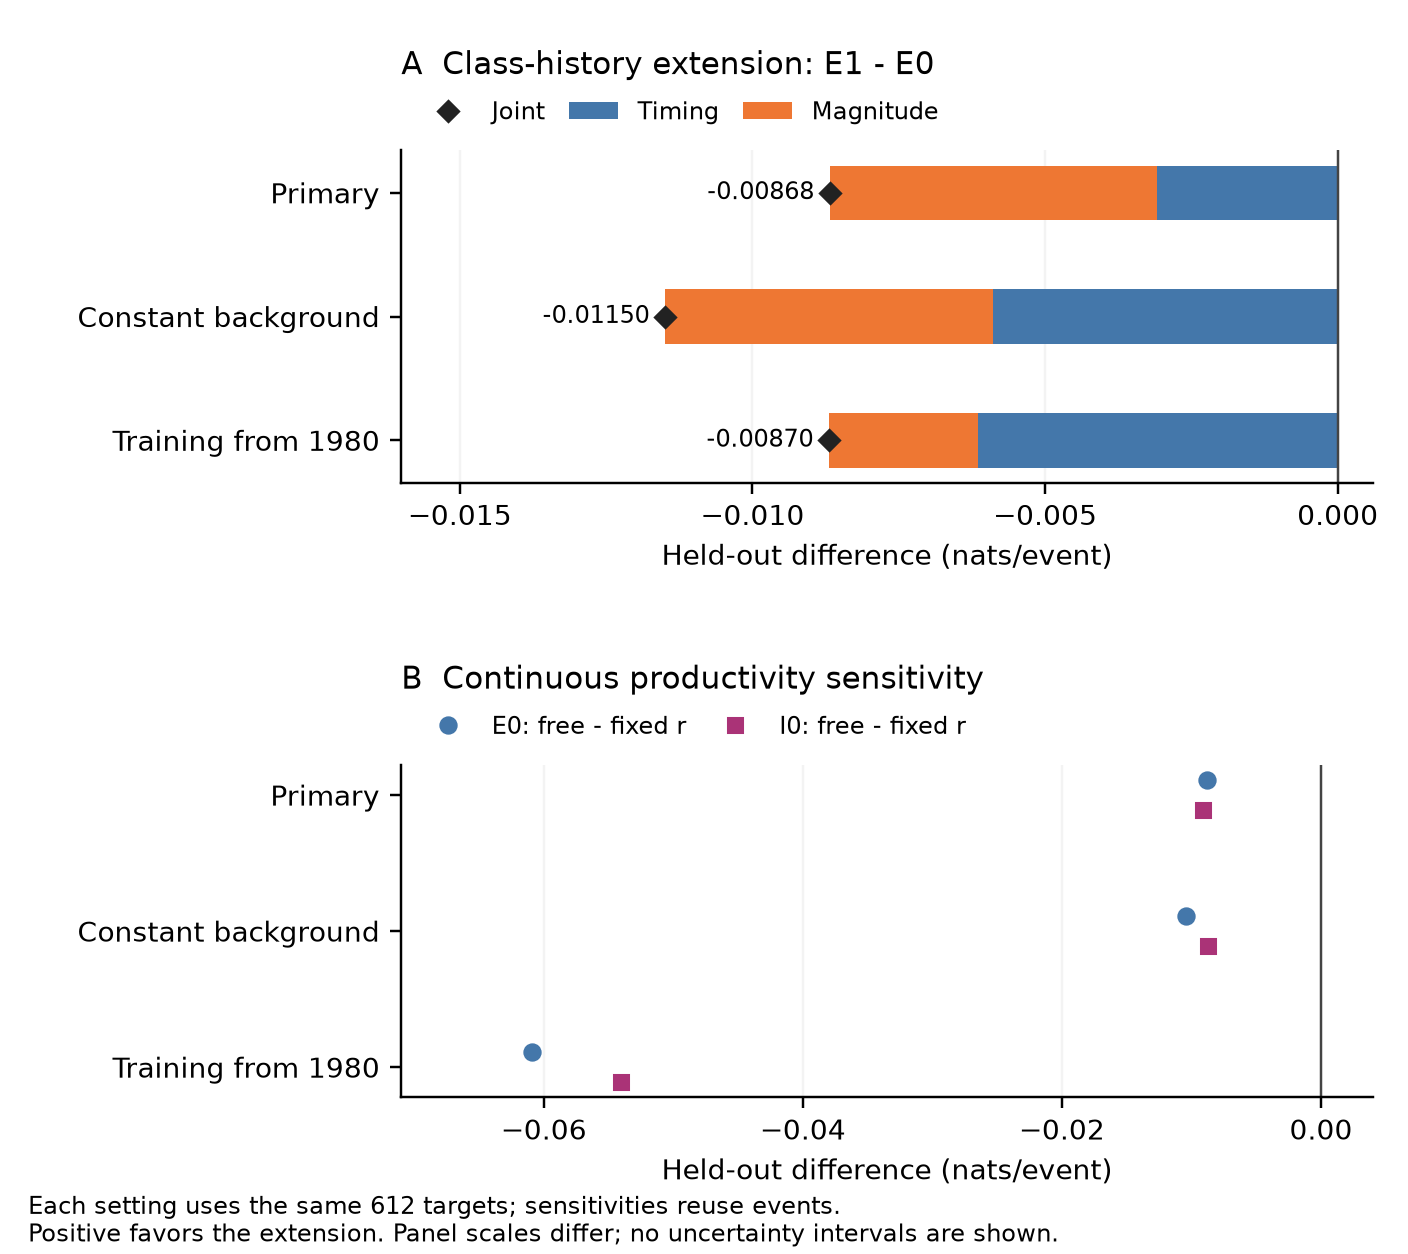
\includegraphics[width=\linewidth]{a2_forecast_comparisons.png}
\caption{Saved aggregate forecast differences. Panel A decomposes the
class-history contrast into timing and magnitude terms; diamonds show their
joint difference. Panel B compares free with fixed productivity in each
ground family. Positive values favor the extension. Each setting reuses
the same 612 targets, the panel scales differ, and no uncertainty intervals
are claimed. Source values are the accompanying reconciled gain tables.}
\label{a2:forecast-figure}
\end{figure}

\section{Interpretation, limitations and disposition}
\label{a2:limits}

The original manuscript, the F nuisance companion and the present
follow-ups address related but distinct questions. The original observed
recipe selected \(r=0.4\) at its first origin and \(r=0.7\) later, with a
different training magnitude-rate estimator. The new comparisons fix
\(r=0.7\) in their reference fits and use a shared training-only
conditional-within-bin estimator. Their matched contrasts are valid
within those separately frozen protocols; they are not corrected entries
in the original paper's predictive table (Chapter~\ref{ch:observed}; Appendix~\ref{app:custody}).

The F checkpoint had 1,528 unknown method outcomes out of 8,596
planned before Stage~2 recovery. Historical counts and accounting bounds
retain their original scope. Neither observed follow-up supplies those
missing null-query results, establishes empirical null size or upgrades a
power comparison. No F fit, bank, calibration or resampling plan was
reopened in this study (Section~\ref{sec:f-continuation}; Appendix~\ref{app:custody}).

The class-history construction is deliberately restricted. The consulted
MDFHP preprint permits class-specific temporal and magnitude-productivity
parameters and bounded class mark distributions, with upper magnitude
10 \citep[Section~2]{DavisBaeumerWangPreprint2024}. Our common-kernel,
low-dimensional \(P(h)\) and source-fertility
contrast, together with an unbounded excess-exponential working law, are
different modelling choices. The conditional summed-intensity identity
depends on those choices. It does not refute the broader class-history
framework, reproduce the authors' Japan or Middle America fits, or
transfer identification and stationarity theorems to a nonlinear
inhibitory family.

All forecast windows had been inspected in earlier research. Training
prefixes overlap and the sensitivity settings reuse the same 612
targets. The results are retrospective exploratory procedure comparisons,
not prospective confirmation or independent replications. Three windows
do not support treating clustered events as independent draws for
standard errors or significance claims. Native magnitude rounding,
mixed magnitude conventions, time-varying detection, missing smaller or
deeper parents, pre-1960 activity and national spatial pooling remain
observation/model assumptions. They were not resolved by these
extensions.

The engineering controls and complete numerical audits make the
implementation inspectable, but do not establish global optima, precise
identification, confidence coverage or power. Positive control examples
show that the fitted pipeline can return gains on particular generating
histories. Equal Perron branching radius did not equate immigrant-weighted
offspring production in the class-active control; different offspring
composition and event counts limit any information-matched comparison.
Sparse profiles and near-training-equivalent candidate spreads retain
their descriptive meanings.

The negative forecast results do not establish that physical inhibition
is absent. Nor do lower fitted slopes establish that \(r=0.7\) is
physically wrong, or show that the earlier negative fertility contrasts
were caused by that fixed value. The cross-run pattern motivates a
possible compensation interpretation, while joint estimation of the
fertility/association extension with free \(r\) remains unperformed.
The persistence of \(E0\)'s forecast advantage over \(I0\) is specific
to the tested recipes and windows.

Both investigations are therefore retained at their respective negative
checkpoints. The fixed-\(r\) \(E0\) candidate remains the predictive
reference for these follow-up comparisons. Broken-slope, saturation,
spatial-locality and independent-data extensions were outside their
executed scope. A future study would require a separately justified
question, information set and protocol, rather than further tuning of
these already examined forecast windows.

\section{Evidence and reproducibility scope}
\label{a2:repro-scope}

The companion records exact protocol, source, score-table and review
identities. The deterministic editorial reconciliation recomputes display
contrasts and counts from saved aggregate/model records using an explicit
hash-bound input list. It does not regenerate scientific histories,
refit models, recalibrate tests or repeat the raw-catalogue auditors.

The original history audit and the later source-reconstructed productivity
audit have different recorded scopes. The latter evaluated all saved
candidates using independently reconstructed geometry rather than merely
checking cache hashes and scoring from production arrays. Their passed
receipts are evidence about the executed checks, not certification of
every mathematical or scientific assertion.

The first API harness and first fresh-control saved-auditor interface
failures in the productivity study remain preserved with their repairs.
The successful append-only auditor corrected terminal-record model-name
extraction without changing scientific fits or tolerances. No control
history was redrawn and no observed outcome refitted in that repair.
A cosmetic profile-figure correction changed marker visibility only.
Earlier engineering adjustments in the history study likewise remain
in its own execution evidence.

The public companion contains the reviewed source and derived score and
parameter display packet, source/result identities and accepted figures.
The exact public manifest identifies its membership. Raw observed catalogue rows and
geometry caches, external article PDFs, private literature inputs and
provider conversations are excluded. Complete raw-geometry replay
requires the separately held matching input and cache files; frozen
absolute paths require an explicit reviewed relocation mapping.
Availability of a compact saved-result packet does not imply availability
of every historical dependency.
The accompanying historical-execution excerpt retains mandatory-start
completion slots and the relevant saved auditor counts and geometry-check
flags, with selectors and original source hashes. It reports prior checks;
no raw-source reconstruction was repeated for this addendum. A separate
boundary inventory distinguishes prescribed coordinates from estimated
constraint hits.

Likelihood and analytic-gradient evaluation run in C++; Python handles
geometry, optimization orchestration, artifact analysis and audits.
MATLAB was unnecessary for these two predictive follow-ups. An earlier
reference-kernel bridge and inspected upstream source are attributed
separately from the independently implemented repeated likelihood.
Existing contributor and AI-assistance disclosures are retained;
computational-agent review is distinct from independent external
human peer review.



\subsection{Data, source and software attribution}

The GeoNet catalogue DOI identifies a continuously updated data resource;
the analyses use the frozen archived selection, whose processed SHA-256 is
\begin{center}\small
\nolinkurl{feacccb7581d1c4c33f88874cd6b198c41639da6930a7fc35e46f910a594fb3e}.
\end{center}
We acknowledge GeoNet and its programme sponsors for the data underlying
the studies. Native magnitude scales and the original selected values are
retained. Neither source citations nor matching archive hashes validate
homogeneity or catalogue completeness.

The Otago implementation was inspected at the separately identified
\emph{MDFHPCode} source commit \citep{MDFHPCode}. An earlier feasibility
reference-kernel bridge is distinct from the independently implemented
finite-mixture objective used in the two predictive follow-ups. Its source
context includes Garrappa's numerical Mittag-Leffler work
\citep{Garrappa2015}. We do not redistribute the upstream general contour
implementation, reference-paper PDFs, upstream binaries or private
literature packet. Citation of a paper and compliance with a code file's
licence are separate responsibilities; no claim of a full MATLAB optimizer
reproduction follows from the reference check.

The recorded pilot environment used Python 3.13.4, NumPy 2.2.6 and SciPy
1.15.3. NumPy, SciPy and Matplotlib are credited for their actual array,
optimization and display roles \citep{Harris2020,Virtanen2020,Hunter2007}.
Repeated likelihood and analytic-gradient work was compiled C++; changing
the compiler or rebuilding a library creates a new binary identity. The
editorial build uses Tectonic 0.17.0, and its source, tool and figure hashes
are recorded separately from the scientific execution records. Font and
package resources were not snapshotted as a byte-identical historical
environment.

\subsection{Versioned evidence and saved-display replay}

The history record is
\nolinkurl{magnitude_prediction_20261023T222049Z}, at checkpoint
\nolinkurl{stop_no_robust_joint_gain}. The productivity record is
\nolinkurl{productivity_slope_20261024T023501Z}, at checkpoint
\nolinkurl{stop_no_robust_productivity_gain}. These local records are
identified by their saved protocol, source and output hashes. The companion
data provide complete case/model score and parameter tables, the saved-count
derivation for the 164 earlier selected parents, and the aggregate values
and cell provenance used here; no
journal DOI or already-published remote record is invented for either run.

Portable display replay reads only the supplied aggregate JSON/CSV packet
and writes to new output directories. It can recreate the gain tables and
figures without fitting models, generating histories or accessing event
rows. The source/replay guide explains commands and omitted dependencies.
The annotated \texttt{scientific\_settings.json} excerpt retains the
kernel/stress constants, solver and profile policies, and continuation
gates, with the original producer-protocol hashes. It is not a replacement
frozen protocol. For the Mittag-Leffler representation, the serialized
\(p=1.3\) field is inactive rather than an additional fitted kernel shape.
This is different from repeating the original raw-data auditors or
reconstructing every historical scientific source epoch. Original
absolute-path producer records retain their old identities; a relocated
raw-data replay needs an explicit reviewed mapping and matching private
inputs.

\begin{figure}[p]
\centering
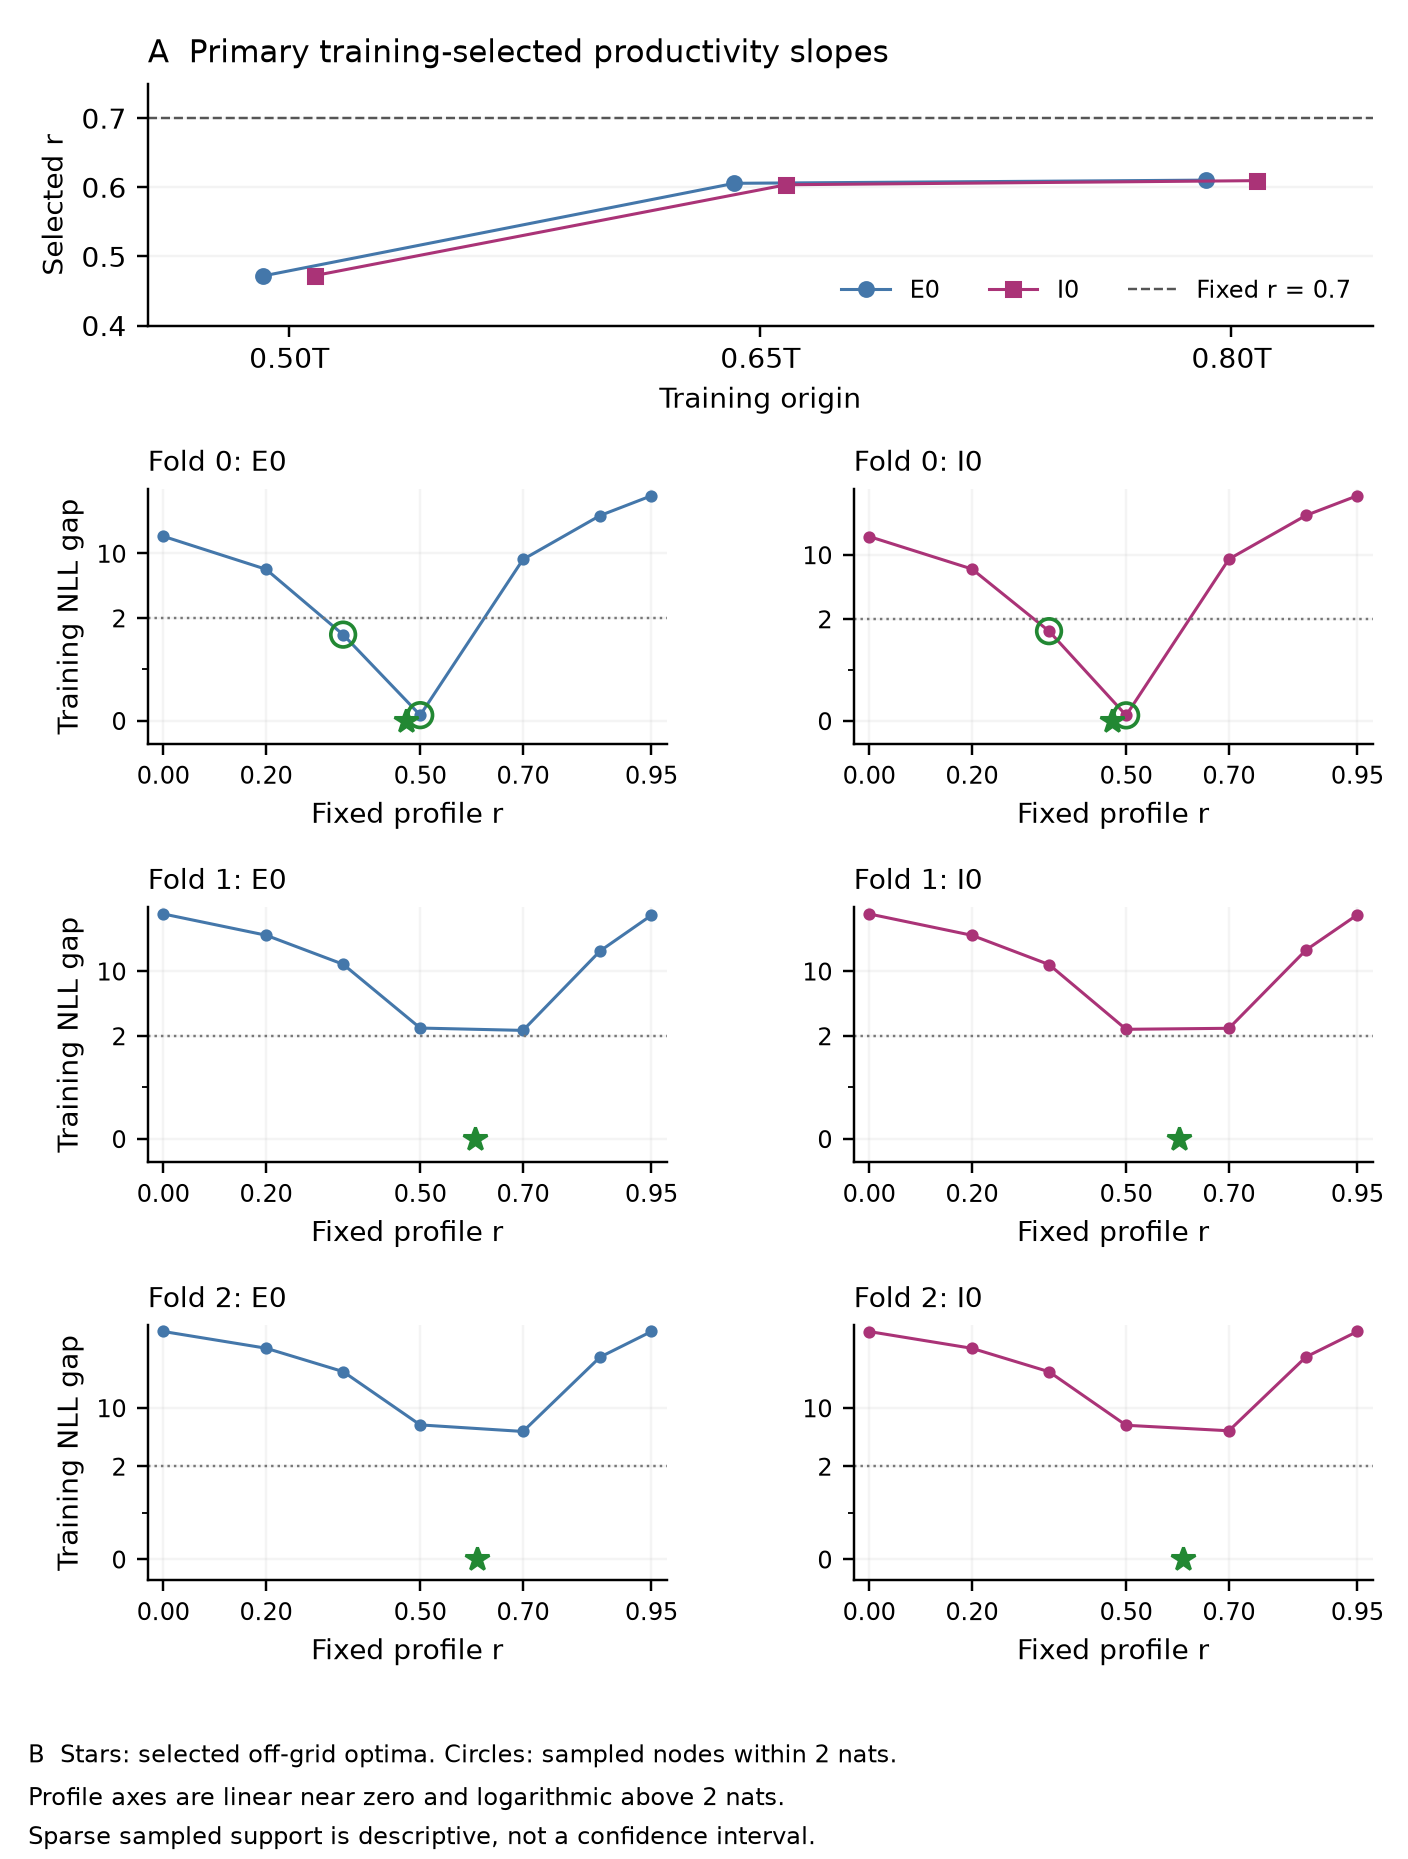
\includegraphics[width=\linewidth,height=.78\textheight,keepaspectratio]{a2_productivity_profiles.png}
\caption{Primary training-selected productivity ratios and the seven-node
descriptive profiles. Stars show selected off-grid optima; circles identify
sampled points within two nats. The profile vertical axes are linear near
zero and logarithmic above two nats. Empty sampled support in four panels
does not define an empty confidence interval. All values are saved training
results; profile forecasts did not select parameters.}
\label{a2:profile-figure}
\end{figure}

\noindent The complete magnitude-extension fold accounting is retained in \hyperref[app:audit09-magnitude-folds]{Appendix~\ref{app:audit09-magnitude-folds}}.

\section{Exposure orthogonalization and the Stage A coarse-kernel comparison}
\label{sec:stage-a}
Let $w_l>0$ be the normalized training exposure quadrature weights and write
$\bar x=\sum_lw_lx_{\mathrm{trend}}(t_l)$, $\bar G=\sum_lw_lG_l$. Provided
$V_x=\sum_lw_l(x_{\mathrm{trend}}(t_l)-\bar x)^2>0$, define
\[
 \gamma_1=\frac{\sum_lw_l(x_{\mathrm{trend}}(t_l)-\bar x)(G_l-\bar G)}{V_x},\qquad
 \gamma_0=\bar G-\gamma_1\bar x,\qquad R=G-\gamma_0-\gamma_1x_{\mathrm{trend}}.
\]
Then $\sum_lw_lR_l=\sum_lw_lx_{\mathrm{trend}}(t_l)R_l=0$ algebraically. The coefficients
are estimated from training exposure only and frozen for prediction and
order-32 checking. Refitting them on the verification grid would change the
model. Degenerate exposure variance invalidates the two-coordinate projection;
zero residual variance reports redundancy rather than identification.
The unrestricted map is exact:
\[
 \widetilde a=a-\eta\gamma_0,\quad
 \widetilde d=d-\eta\gamma_1,\qquad
 a=\widetilde a+\eta\gamma_0,\quad
 d=\widetilde d+\eta\gamma_1.
\]
Thus $a+dx_{\mathrm{trend}}-\eta G=\widetilde a+\widetilde d x_{\mathrm{trend}}-\eta R$ at every time.
Equal numerical boxes in these coordinates describe different constrained
families; mapped floors are admissible only when all destination restrictions
hold, without clipping. An $\eta$-only ridge is invariant under this map.
Raw $d=0$ differs from residual $\widetilde d=0$. The residual can be negative,
so the detrended background may locally exceed its nominal undepleted level.
Exposure orthogonality is not likelihood-score orthogonality: event scores
contain $B/\lambda$, information involves $B^2/\lambda$, and projection onto
$(1,x_{\mathrm{trend}})$ does not remove dependence on the excitation-amplitude score.

For $B=\exp(\widetilde a+\widetilde d x_{\mathrm{trend}}-\eta R)$ and
$\lambda=B+nH$, let $J$ be complete productivity-weighted trigger exposure.
The timing negative log likelihood and gradient are
\begin{align*}
 L&=\sum_lq_lB_l+nJ-\sum_i\log\lambda_i,\\
 L_{\widetilde a}&=\sum_lq_lB_l-\sum_i B_i/\lambda_i,&
 L_{\widetilde d}&=\sum_lq_lx_{\mathrm{trend}}(t_l)B_l-\sum_i x_{\mathrm{trend}}(T_i)B_i/\lambda_i,\\
 L_n&=J-\sum_iH_i/\lambda_i,&
 L_\eta&=-\sum_lq_lR_lB_l+\sum_iR_iB_i/\lambda_i.
\end{align*}
The raw formulas replace $R$ by $G$. At $n=0$, $L_n$ remains well defined;
at $\eta=0$, values and shared-coordinate gradients must nest using a common
integration branch or an explicitly controlled numerical seam.

Stage A selected Omori triggering by training excitation-only fits on the
nine-point grid $c\in\{0.1,1,10\}$ days and $p\in\{1.1,1.3,1.7\}$.
The selected kernel was frozen for its excitation/inhibition pair. The stress
survival law and $r=0.7$ remained fixed. This is a restricted coarse-grid
procedure, distinct from the historical continuously refined Omori fit and
the later continuous Extension O.
\section{Stage A saved evidence and interpretation}


All planned procedures are complete and independently audited. A negative predictive result is a completed Stage A result.

\subsection{Aggregate held-out comparisons}


The variants reuse the same targets. Mark-score differences cancel; timing is the event plus compensator contribution. In primary, exposure orthogonalization changes the pooled ML inhibition contrast by only \(-0.000045575\) nats, from \(-18.186415\) to \(-18.186460\) nats. The raw interior optimum maps feasibly into the orthogonal box; better Gram conditioning therefore does not change the represented optimum materially.





\subsection{Interpretation limits}


Orthogonalization is an invertible unrestricted coordinate transformation. Identical boxes in raw and transformed coordinates define different constrained families, including intercept constraints. The projection removes exposure drift; it does not establish likelihood-score orthogonality. Constant-background restrictions have different meanings in the two coordinates.

Omori parameters were selected by training E0 on the fixed nine-point grid and shared within each excitation/inhibition pair. The ML stress survival law and r=.7 remained fixed. This is not exact replication of Iteration27 continuous kernel/productivity selection.

Historical Fold0 raw inhibition loss around -16.99 nats is contextual. Compare against the newly recomputed raw baseline and retain differences due to nuisance/optimizer estimation. Selected parameters, mapped feasibility, bound flags, training-only coefficients and Gram diagnostics are saved in results/analysis.

Previously inspected chronological windows and one regional catalogue support descriptive predictive comparisons only. No event-iid confidence intervals, Wilks boundary claims, global-optimum certificate or physical-causality assertion. Stage A preceded the completed Stage B and C studies reported later in this volume.

\subsection{Audit}


The independent auditor reconstructed local raw rows, nuisance estimates, kernels, quadrature and projection; checked every saved candidate and solver return, exact floors, all planned start slots and aggregate score entries. Internal optimizer line-search iterates were not all serialized.

\subsection{Fold0 reconciliation}


Historical rawI-minus-E0: -16.988778741 nats; recomputed rawI-minus-E0: -16.988735123; difference: +0.000043618.
Orthogonal ML inhibition minus E0: -16.988768914; orthogonal-minus-raw improvement: -0.000033791 nats.
Matched Omori inhibition minus its E0: -16.404033164; Omori E0 minus ML E0: -3.210666185; combined orthogonal Omori minus ML E0: -19.614699350 nats.
These are arithmetic contrasts of separately trained constrained procedures, not a causal decomposition.




\noindent The stage A complete fold score accounting is retained in \hyperref[app:audit09-stage-a-folds]{Appendix~\ref{app:audit09-stage-a-folds}}.

\subsection{Stage A complete aggregate score accounting}
Comparison keys are local to this table. 
\begin{description}
\item[AG1] \path{I0_raw_ml-E0_ml}
\item[AG2] \path{I0_orth_ml-E0_ml}
\item[AG3] \path{I0_orth_ml-I0_raw_ml}
\item[AG4] \path{E0_omori-E0_ml}
\item[AG5] \path{I0_orth_omori-E0_omori}
\item[AG6] \path{I0_orth_omori-I0_orth_ml}
\item[AG7] \path{(I0_orth_omori-E0_omori)-(I0_orth_ml-E0_ml)}
\end{description}

\noindent The stage A aggregate sensitivity accounting is retained in \hyperref[app:audit09-stage-a-sensitivity]{Appendix~\ref{app:audit09-stage-a-sensitivity}}.

{\small
\setlength{\tabcolsep}{3pt}
\begin{longtable}{lrrrrrr}
\caption{Stage A complete aggregate score accounting; primary. Total nats unless stated otherwise. Positive favors the candidate. The same 612 targets enter each aggregate; positive-fold counts are out of three.}\label{tab:AG-primary}\\
\toprule
Key & $\Delta Q$ & $\Delta C$ & Timing & $\Delta M$ & Joint & Joint/event\\\midrule
\endfirsthead
\toprule
Key & $\Delta Q$ & $\Delta C$ & Timing & $\Delta M$ & Joint & Joint/event\\\midrule
\endhead
AG1 & -40.854975 & 22.668560 & -18.186415 & 0.000000 & -18.186415 & -0.029716\\
AG2 & -40.855042 & 22.668582 & -18.186460 & 0.000000 & -18.186460 & -0.029716\\
AG3 & -0.000068 & 0.000022 & -0.000046 & 0.000000 & -0.000046 & -0.000000\\
AG4 & -38.017200 & -0.154092 & -38.171292 & 0.000000 & -38.171292 & -0.062371\\
AG5 & -36.772664 & 20.496091 & -16.276573 & 0.000000 & -16.276573 & -0.026596\\
AG6 & -33.934822 & -2.326583 & -36.261405 & 0.000000 & -36.261405 & -0.059251\\
AG7 & 4.082379 & -2.172491 & 1.909887 & 0.000000 & 1.909887 & 0.003121\\
\bottomrule
\end{longtable}
}

\noindent The stage A training exposure geometry is retained in \hyperref[app:audit09-stage-a-geometry]{Appendix~\ref{app:audit09-stage-a-geometry}}.

\section{Stage B: common and parent-class temporal scales}
\label{sec:stage-b}
For a pinned positive mixture with $\sum_mw_m=1$, use $s=\log\tau$ and
$a_m=\lambda_m e^{-s}$ to write
\[
 k_s(u)=\sum_mw_ma_me^{-a_mu},\qquad S_s(u)=\sum_mw_me^{-a_mu}.
\]
Every scale preserves unit mass; the parent's observed class selects its
entire kernel. The prospective range was $\tau\in[0.001,20]$ days,
including subhour scales. This is no cutoff on the retained parent history.
At $y=a_mu$,
\[
 \partial_s k_s(u)=\sum_mw_ma_me^{-y}(y-1).
\]
For a parent's finite-window lag interval $[L,U]$,
\begin{align*}
 J_k(s)&=\sum_mw_me^{-a_mL}\{-\operatorname{expm1}[-a_m(U-L)]\},\\
 \partial_sJ_k&=\sum_mw_m\{a_mLe^{-a_mL}-a_mUe^{-a_mU}\}.
\end{align*}
Productivity weights multiply these expressions; all earlier parents and quiet
exposure remain. Lags, rather than edited cached kernel values, define dynamic
evaluation. The fixed-scale, common-free and class-free models respectively
fix both scales to one day, estimate a common scale, and estimate two parent
scales. All use $h=\delta=0$, fixed $r=0.7$ and the common training magnitude
law. The common gradient is the sum of class gradients on the diagonal;
at $n=0$ all scale derivatives vanish and the scales are unidentified.

The optional association family preserves the original Perron normalization:
\[
 \lambda_i=p_iB+\frac n{\rho(h)}\sum_jP_{ij}(h)H_j,\qquad
 \Lambda=B+\frac n{\rho(h)}(H_0+H_1).
\]
Unit temporal mass makes $\rho$ independent of the scales. Column stochasticity
still cancels target redistribution even with different parent kernels.
At fixed effective amplitude $n/\rho(h)$, timing is invariant to $h$ wherever
the map remains feasible; conditional marks can change. Joint refitting and
box constraints may indirectly change timing. No target-class temporal family
was introduced to evade this identity.

For $\Gamma=n/\rho$, $T_i=\sum_jP_{ij}H_j$ and
$e_i=p_iB+\Gamma T_i$, the optional joint negative log likelihood is
\[
 L=\int B+\Gamma(J_0+J_1)-\sum_i\log e_i
   -\sum_i\{\log f_\beta(q_i)-\log p_i\}.
\]
Its scale gradient is
$L_{s_j}=\Gamma J'_j-\sum_i\Gamma P_{ij}H'_j/e_i$ and
\[
 L_h=-\Gamma\frac{\rho'}\rho(J_0+J_1)
 -\sum_i\frac{\Gamma\{\sum_jP'_{ij}H_j-(\rho'/\rho)T_i\}}{e_i},
 \quad P'_{ij}=\mathbf1_{i=j}-p_i.
\]
The nuisance $\beta,p_i$ are training-frozen. At $n=0$, association and scale
gradients vanish. All prescribed starts and exact nested floors must resolve;
a finite candidate cannot replace an incomplete start. Near-training-equivalent
candidates within $4\times10^{-4}$ NLL receive full forecast checks with spread
strictly below $0.01$ nats/event.
\section{Stage B audited results, historical bridge and failed association gate}


Allowing one common Mittag-Leffler timescale improves pooled event-timing forecasts in all three retained windows. Additional parent-class timescales give a small positive aggregate gain, but improve only one window against the common-scale model. The predeclared association gate therefore fails, and no observed h model was fitted. This is a completed gated investigation, not a negative result for the unexecuted h branch.

\subsection{Audited comparisons}


All nine observed fit procedures and 72 prescribed starts completed. The independent raw-row audit reconciled 90 candidates and 72 solver returns, with no failed finite solver returns. The two fixed-seed engineering histories also completed eight procedures/64 starts, including the optional h engine. Near-optimal forecast stability and source/input integrity gates passed.

The 612 targets occur in disjoint chronological windows containing 203, 155 and 254 events; their training prefixes overlap. All three observed models use fixed r=0.7, the same training-only beta per case, h=0 and the same magnitude density. Mark differences cancel up to floating-point roundoff, so timing and joint gains coincide.


Here the historical E field is the ground event-log-intensity contrast, denoted $\Delta Q$ in this volume and C is the baseline-minus-candidate compensator, so $\Delta Q+\Delta C$ equals timing. Timing plus the conditional-mark contrast equals joint score. These are event-weighted sums divided by 612, rather than unweighted averages of fold rates.


The common-scale gain is consistent across these windows, although Fold 0's gain is only 0.077011 nats. The class-specific aggregate is positive, not a net loss. Its inconsistency against the stronger common-scale comparator is the reason the next branch stops. Winning two windows against the fixed tau=1 baseline is not the declared gate.

\subsection{Scale and selection limits}


All selected parameters are interior to their prescribed bounds. The allowed tau range was 0.001 to 20 days, including subhour values, but none of the observed fitted scales is subhour. There is no lower-bound truncation explanation for these selected estimates and no bound expansion was performed.

Class 0 means 5.0$\leq$M<5.5 and class 1 means M$\geq$5.5. The kernels attach to the parent's class. The fitted ordering changes: class 0 is faster in Fold 0 but slower in Folds 1 and 2. These fits do not establish a stable physical magnitude ordering of aftershock timescales. Tau is a normalized-kernel scale, not a finite aftershock-duration cutoff, and is not interchangeable with Omori c.

Training NLL improves under exact nested floors. The additional class-specific training gains against the common model are approximately 0.012055, 1.867655 and 5.248592 nats, yet two held-out windows lose. Neither training improvement nor passing near-optimal forecast checks certifies physical scale identification or a global optimizer.

\subsection{Optional association branch}


The prospective rule required class-specific h=0 timing to exceed common-scale timing by more than 0.0001 total nats in at least two windows, after complete fitting, independent audit and forecast stability. Only Fold 1 qualifies. The audited gate is false: zero of the conditional three observed h procedures/24 starts were executed. The h code, derivatives and synthetic engineering were validated before observing this decision; engineering validation is not observed evidence for or against association.

The optional mathematical family preserves the legacy Perron normalization. With parent-class kernels, summing the column-stochastic transition matrix still gives ground intensity B+(n/rho(h))(H0+H1). Association h adds no new direct temporal shape conditional on observed parent history; its scalar n/rho effect is already an excitation-amplitude coordinate. At fixed effective amplitude, timing is invariant to h, while conditional mark probabilities can change. No target-class kernels or post-gate model family were introduced.

\subsection{Historical Omori reference}


The immutable historical Omori total is -990.170063 joint nats. The new fixed-scale, common-scale and class-scale procedures have raw joint totals of approximately -984.684158, -977.300484 and -976.292651. Their raw differences from historical Omori are +5.485905, +12.869579 and +13.877412 nats, respectively.

These are descriptive cross-procedure comparisons, not matched kernel-only gains. Historical selected productivity ratios are [0.4,0.7,0.7], whereas B fixes 0.7 throughout; only Fold 0 has that productivity mismatch. All three historical beta estimates use a different global-MLE convention. Beta also enters productivity weights, so this difference affects timing as well as magnitude scores. Historical Omori also used its own continuous shape/scale selection.

For common free tau, the raw historical difference splits into +10.389214 timing and +2.480366 magnitude nats. Magnitude terms therefore cannot be cancelled across those recipes. The matched B free-scale gain remains +7.383674 nats; the larger historical difference cannot be attributed solely to freeing tau. No prior Omori fit was rerun or overwritten, and no new matched Omori model was fitted.

\subsection{Delimited conclusion}


The supported result is a modest, consistent timing gain from a common free ML scale in this bounded pooled procedure. Parent-class scales add a smaller positive aggregate but fail the predeclared across-window continuation criterion. Optional h remains untested on observed data.

This retains the original regional B design despite earlier spatial results; it is not a combined spatial-temporal validation or an independently replicated catalogue. All windows were previously examined. No physical causality, event-iid confidence interval, Wilks boundary inference, global-optimum certificate, alternative bounds or automatic further study is warranted.


\noindent The stage B complete fold score accounting is retained in \hyperref[app:audit09-stage-b-folds]{Appendix~\ref{app:audit09-stage-b-folds}}.

\subsection{Stage B complete aggregate score accounting}
Comparison keys are local to this table. 
\begin{description}
\item[BG1] \path{E0_tau_free-E0_tau1}
\item[BG2] \path{E1_tau_class-E0_tau_free}
\item[BG3] \path{E1_tau_class-E0_tau1}
\end{description}

{\small
\setlength{\tabcolsep}{3pt}
\begin{longtable}{lrrrrrrr}
\caption{Stage B complete aggregate score accounting; primary. Total nats unless stated otherwise. Positive favors the candidate. The same 612 targets enter each aggregate; positive-fold counts are out of three.}\label{tab:BG-primary}\\
\toprule
Key & $\Delta Q$ & $\Delta C$ & Timing & $\Delta M$ & Joint & Joint/event & Positive folds\\\midrule
\endfirsthead
\toprule
Key & $\Delta Q$ & $\Delta C$ & Timing & $\Delta M$ & Joint & Joint/event & Positive folds\\\midrule
\endhead
BG1 & 4.405481 & 2.978194 & 7.383674 & 0.000000 & 7.383674 & 0.012065 & 3\\
BG2 & 5.297977 & -4.290144 & 1.007833 & 0.000000 & 1.007833 & 0.001647 & 1\\
BG3 & 9.703458 & -1.311951 & 8.391507 & 0.000000 & 8.391507 & 0.013712 & 2\\
\bottomrule
\end{longtable}
}

\noindent The stage B selected temporal scales are retained in \hyperref[app:audit09-stage-b-scales]{Appendix~\ref{app:audit09-stage-b-scales}}.

\section{Extension O: continuously tuned, kernel-matched inhibition}

The Omori--Utsu temporal law is a standard aftershock-decay model \citep{Utsu1995}; the comparisons below concern its declared fitted implementation and bounds.
\label{sec:extension-o}
For $u\geq0$, use the normalized Omori density and survival
\[
 k(u)=\frac{p-1}{c}(1+u/c)^{-p},\quad
 S(u)=(1+u/c)^{1-p},\qquad c>0,\ p>1.
\]
With $s=\log c$, $A(u)=\log(1+u/c)$ and $v=u/(c+u)$,
\[
 \partial_s\log k=-1+pv,\quad
 \partial_p\log k=(p-1)^{-1}-A,\quad
 \partial_sS=(p-1)vS,\quad \partial_pS=-AS.
\]
Parent exposure is $J=S(L)-S(U)$ and its derivatives use the same endpoint
differences; stable evaluation uses $S(L)\{-\operatorname{expm1}[(1-p)
(A(U)-A(L))]\}$. No lag truncation is used. The prospectively fixed bounds
are $c\in[10^{-4},20]$ days and $p\in[1.01,2.5]$. These numerical domains
do not identify physical duration or justify an outcome-dependent expansion.
For $z\in\{s,p\}$ the additional timing gradient is
\[
 L_z=n\sum_k\kappa_k\partial_zJ_k
          -\sum_i\frac{n\partial_zH_i}{\lambda_i}.
\]
The stress feature remains the original unit-scale ML survival history and
has no $c,p$ derivative. Both kernel gradients vanish at $n=0$.

The primary excitation fit selects $(c,p)$ by training NLL and shares those
values exactly with raw and orthogonal matched inhibition. The jointly tuned
orthogonal inhibitory fit is secondary. Exact Poisson/nested floors and the
sealed coarse Stage A excitation point are reevaluated in the new objective;
old scores are neither overwritten nor substituted. Every procedure uses its
prescribed starts, with training-only selection and the saved forecast-stability
gate. The same coordinate map and feasibility requirements from Stage A apply.

For the raw inhibited engineering law, the valid thinning envelope is the
undepleted background plus excitation; current inhibited intensity is not a
monotone envelope because stress may recover between events. Independent time
and mark streams, rejection records, caps and unreplaced failed histories are
part of engineering eligibility. A matched training-selected kernel need not
equal the generating kernel; no invalid truth-containment claim follows.
\section{Extension O audited results and sensitivity interpretation}


Continuously training-tuned Omori excitation improved held-out timing over the fixed ML baseline in all three primary windows. Stress inhibition still reduced aggregate held-out scores under the same E-selected Omori kernels. The primary matched orthogonal contrast lost 14.137174 nats across 612 targets, and the secondary jointly tuned inhibitory model lost 11.803237 nats. This is a negative result for the implemented bounded stress-depletion procedures, alongside a positive result for temporal-kernel tuning.

All 45 planned procedures and 360 prescribed starts completed; the independent raw-row audit reconciled 456 candidates and 360 solver returns and found stable near-optimal forecasts. Model selection used training NLL only. Magnitude scores are identical within each case, so every displayed timing difference is also the joint difference.


The matched orthogonal model won only Fold 1 by 0.175158 nats and lost Folds 0 and 2. The jointly tuned inhibitory model lost all three primary windows. Its 2.333937-nat aggregate improvement over matched orthogonal inhibition is secondary; it does not turn the inhibitory versus excitatory comparison positive.

For E\_omori minus E\_ml, the event-log-intensity gain was 17.242145 nats and the compensator contribution was -5.036642 nats, giving +12.205503. For matched orthogonal inhibition minus E\_omori, the event contribution was -37.002313 and the compensator contribution +22.865140, leaving -14.137174. Lower exposure could not offset lost event intensity.

The training-selected primary excitation kernels are reported in Table~\ref{tab:o-kernels} in Appendix~\ref{app:audit09-extension-o-kernels}.


These c and p estimates are interior to the prospectively fixed bounds. The short selected c values explain why the earlier coarse grid with minimum c=0.1 day did not adequately search this continuous family. This is a scale parameter of a heavy-tailed kernel, not an estimated physical recovery duration. Stress itself still uses the original fixed ML survival kernel; only triggering was continuously tuned.

Orthogonalization did not rescue the primary loss. In Fold 0 raw inhibition reached its raw d=2 upper boundary. Its selected point maps feasibly into orthogonal coordinates, while the orthogonal optimum maps back to raw d=2.114439 and lies outside the raw box. The orthogonal fit improves training NLL by only 0.005858 nats but loses a further 0.361471 test nats. In Folds 1 and 2 the selected points map feasibly both ways and their forecasts agree up to numerical optimization differences. Thus the small primary difference between raw and orthogonal procedures is explained by a changed bounded parameter domain, rather than a new unrestricted model space. Exposure orthogonality is not likelihood-score orthogonality.

The constant-background sensitivity fixes raw d=0 or detrended d\_tilde=0 respectively. These are different restrictions; all selected mapped raw/orth constant-case points violate the destination constant restriction. Their contrast cannot be interpreted as pure reparameterization. The post-1980 variant changes the training window and its projection/nuisance estimates, while retaining full prior event history.


Omori excitation wins all three windows in each sensitivity variant. Every inhibitory aggregate remains negative. Constant-background detrended inhibition improves over raw inhibition by 5.449474 nats, but still loses 8.796918 nats against its matched excitatory comparator. The same test events are reused across variants and must not be pooled as 1,836 independent targets.

Within this bounded, regionally pooled fixed-productivity family, inhibitory failure therefore persists after replacing the inferior fixed ML trigger with continuously tuned Omori excitation. It cannot be attributed solely to that fixed-trigger choice or solely to the raw trend boundary. This does not establish that physical stress inhibition is absent, and it does not test continuous spatial stress or a joint spatial/temporal extension. The historical Iteration 27 Omori result uses a different nuisance recipe, including the Fold 0 productivity ratio and training magnitude estimator; the present gain is a new internally matched comparison, not a numerical reproduction of that historical score.

The catalogue and windows were previously inspected, and three chronological tests provide limited robustness evidence. No event-iid intervals, boundary Wilks claims, physical-causality conclusions or global-optimum certificate follow. S was designed and frozen before these outcomes; its launch is governed by correctness and resource admission, not this score direction.

Exact per-window scores, parameters, boundary flags and both-direction mapping diagnostics are in summary.json. The independent raw-row reconciliation is in observed\_saved\_audit\_v1.json.

\noindent The extension O complete fold score accounting is retained in \hyperref[app:audit09-extension-o-folds]{Appendix~\ref{app:audit09-extension-o-folds}}.

\subsection{Extension O complete aggregate score accounting}
Comparison keys are local to this table. 
\begin{description}
\item[OG1] \path{E_omori-E_ml}
\item[OG2] \path{Iorth_matched-E_omori}
\item[OG3] \path{Iraw_matched-E_omori}
\item[OG4] \path{Iorth_joint-E_omori}
\item[OG5] \path{Iorth_joint-Iorth_matched}
\item[OG6] \path{Iorth_matched-Iraw_matched}
\end{description}

\noindent The extension O aggregate sensitivity accounting is retained in \hyperref[app:audit09-extension-o-sensitivity]{Appendix~\ref{app:audit09-extension-o-sensitivity}}.

{\small
\setlength{\tabcolsep}{3pt}
\begin{longtable}{lrrrrrrr}
\caption{Extension O complete aggregate score accounting; primary. Total nats unless stated otherwise. Positive favors the candidate. The same 612 targets enter each aggregate; positive-fold counts count joint gains exceeding $10^{-4}$ nats out of three. Positive values at or below that threshold are treated as numerical ties.}\label{tab:OG-primary}\\
\toprule
Key & $\Delta Q$ & $\Delta C$ & Timing & $\Delta M$ & Joint & Joint/event & Positive folds\\\midrule
\endfirsthead
\toprule
Key & $\Delta Q$ & $\Delta C$ & Timing & $\Delta M$ & Joint & Joint/event & Positive folds\\\midrule
\endhead
OG1 & 17.242145 & -5.036642 & 12.205503 & 0.000000 & 12.205503 & 0.019944 & 3\\
OG2 & -37.002313 & 22.865140 & -14.137174 & 0.000000 & -14.137174 & -0.023100 & 1\\
OG3 & -36.491541 & 22.715835 & -13.775706 & 0.000000 & -13.775706 & -0.022509 & 1\\
OG4 & -27.179752 & 15.376515 & -11.803237 & 0.000000 & -11.803237 & -0.019286 & 0\\
OG5 & 9.822562 & -7.488625 & 2.333937 & 0.000000 & 2.333937 & 0.003814 & 1\\
OG6 & -0.510772 & 0.149304 & -0.361468 & 0.000000 & -0.361468 & -0.000591 & 0\\
\bottomrule
\end{longtable}
}

\noindent The extension O selected continuous kernels are retained in \hyperref[app:audit09-extension-o-kernels]{Appendix~\ref{app:audit09-extension-o-kernels}}.

\section{Engineering witnesses and constrained-map diagnostics}
\subsection{Control normalization and saved forecast contrasts}
These are particular fixed engineering realizations. Equal Perron radii do
not equalize immigrant-weighted first-generation production, event counts or
statistical information. In particular the class-active laws can dilute the
offspring contribution. All controls remain visible, including losses, rather
than retaining only successful examples. These tables support implementation
inspection, not calibrated power, bias, coverage or reliable recovery.

\noindent The engineering normalization, forecast, profile and map witnesses are retained in \hyperref[app:audit09-engineering-witnesses]{Appendix~\ref{app:audit09-engineering-witnesses}}.

\subsection{Coarse-grid loss and the later continuous-kernel gain}
The coarse Stage A excitation-only Omori procedure lost to its matched ML
reference in every aggregate setting: primary -38.171292, post-1980 -15.005799 and constant-background -43.433403 nats.
Every excitation-selected scale in Table~\ref{tab:a-coarse-kernels} is at the
lower coarse-grid endpoint, $c=0.1$ day. In contrast, continuous Extension O
gained 12.205503 primary nats over its matched ML reference, with all three windows positive.
This is a materially different outcome from the coarse-grid loss. The continuous
primary selected scales lie below the earlier grid, but these results compare
bounded fitted procedures; they do not identify a universal kernel ranking.

\noindent The stage A selected coarse-grid kernels are retained in \hyperref[app:audit09-coarse-kernels]{Appendix~\ref{app:audit09-coarse-kernels}}.

\subsection{Engineering-clock and evaluation scope}
Stage B's two engineering laws fixed a common scale of $0.02$ day or parent
scales $(0.005,0.5)$ day, with log immigration $a=\log(0.4)$, $d=0$,
$n=0.2$, $\beta=2.85$, $r=0.7$, a $500$-day horizon and training ending at
day $350$. The horizon was fixed before generation to retain expected
immigration while reducing binary64 clock spacing relative to the earlier
$5000$-day engineering design. It did not rescale observed data or change the
absolute scale bounds. In the uninhibited constant-background controls,
inversion of the exact integrated hazard needs no acceptance uniform because
envelope and actual intensity agree. Independent time and mark streams,
retained sampled versus actual binary64 elapsed times and fail-without-jitter
clock rules remain essential. Known synthetic nuisance values and the observed
training-only nuisance adapter have distinct verification roles. The optional
association engine was exercised on both controls before the observed gate;
this supplies no observed evidence about the unexecuted association branch.

The common-scale and parent-scale engineering laws are deliberately fixed
examples, not estimates of a physical ordering. Saved numerical derivatives,
exact nested floors, left limits, complete parent exposure and direct-history
truth checks delimit implementation validity. A repaired control or audit
interface does not authorize replacing failed histories or promoting an
unresolved production outcome. No new engineering computation accompanied
that historical consolidation.

\section{Completed matched magnitude-history experiment}

\label{sec:s02-completed}

\textit{Execution provenance: the original completed campaign passed the saved custody checks and predeclared independent raw sample. Acceptance uses sampled validation, not independent replay of every fit. This edition recovered and verified the original histories, selected fit states and attempt records; it did not rerun the fitting campaign.}

The experiment uses 100 paired forest units and 300 catalogues across persistence settings $h\in\{0,0.5,0.9\}$. The strictly subcritical generator has productivity ratio $r=0$ and reproduction mean $n=0.5$. Each catalogue is fitted by M1, the misspecified $r=0.7$ candidate, and M2, the productivity-matched $r=0$ candidate. Both hold $n=0.5$ and use the same inherited kernels and eight-start null/alternative procedure, fitting the background level, trend and stress coefficient. All 600 procedure--catalogue cases are complete; no seed was redrawn.

M1 is a structural replication arm, not an exact numerical replication of the earlier pilot: the common reproduction mean and strengthened starts are disclosed. M2 matches productivity at $h=0$, but the exact Mittag--Leffler generator and finite 195-mode candidate still differ numerically. It is therefore not described as a literally exact full null law.

\begin{table}[htbp]\centering\setlength{\tabcolsep}{5pt}

\caption{Completed selection counts and descriptive empirical calibration. Selection uses $\mathrm{GLR}>0.001$ and $\hat\eta>10^{-6}$. All entries have 100 resolved catalogues; intervals are 95\% Wilson intervals for selection proportions.}\label{tab:s02-completed}

\begin{tabular}{llrrrr}\toprule

Procedure & $h$ & Selected & Wilson interval & Empirical $h=0$ threshold & Above threshold\\\midrule

M1 & 0.0 & 79/100 & [0.700, 0.858] & 7.665955 & 4/100 \\

M1 & 0.5 & 85/100 & [0.767, 0.907] & 7.665955 & 6/100 \\

M1 & 0.9 & 85/100 & [0.767, 0.907] & 7.665955 & 6/100 \\

M2 & 0.0 & 75/100 & [0.657, 0.825] & 4.629883 & 4/100 \\

M2 & 0.5 & 75/100 & [0.657, 0.825] & 4.629883 & 4/100 \\

M2 & 0.9 & 69/100 & [0.594, 0.772] & 4.629883 & 4/100 \\

\bottomrule\end{tabular}\end{table}

The empirical threshold is the higher empirical 95th percentile of the same 100 $h=0$ GLRs within each procedure. The four strict exceedances among those same controls are a consequence of this in-sample construction and ties, not independent evidence of 5\% Type I error control. Selection by the small fixed GLR cutoff and exceedance of this descriptive threshold are distinct summaries.

\begin{table}[htbp]\centering

\caption{Paired GLR changes from $h=0$ on the same forest units. MC SE is a forest-unit sample standard error.}\label{tab:s02-paired}

\begin{tabular}{llrrr}\toprule Procedure & $h$ & Mean change & Median change & MC SE\\\midrule

M1 & 0.5 & -0.009000 & 0.000000 & 0.146627 \\

M1 & 0.9 & 0.010831 & 0.046652 & 0.416236 \\

M2 & 0.5 & -0.106278 & 0.000000 & 0.098682 \\

M2 & 0.9 & -0.140055 & 0.000000 & 0.118097 \\

\bottomrule\end{tabular}\end{table}

\begin{table}[htbp]\centering

\caption{Within-forest M2 minus M1 GLR contrasts. Negative values favour a larger fitted GLR under the misspecified M1 procedure, not better predictive calibration.}

\begin{tabular}{lrr}\toprule $h$ & Mean GLR contrast & MC SE\\\midrule

0.0 & -1.132859 & 0.425666 \\

0.5 & -1.230138 & 0.423813 \\

0.9 & -1.283745 & 0.211306 \\

\bottomrule\end{tabular}\end{table}

These paired results retain all forest units. Neither the large fixed-cutoff selection proportions nor the descriptive self-calibrated thresholds establish a generally valid test for stress inhibition. There is no independent calibration sample in this threshold comparison.

\begin{figure}[htbp]\centering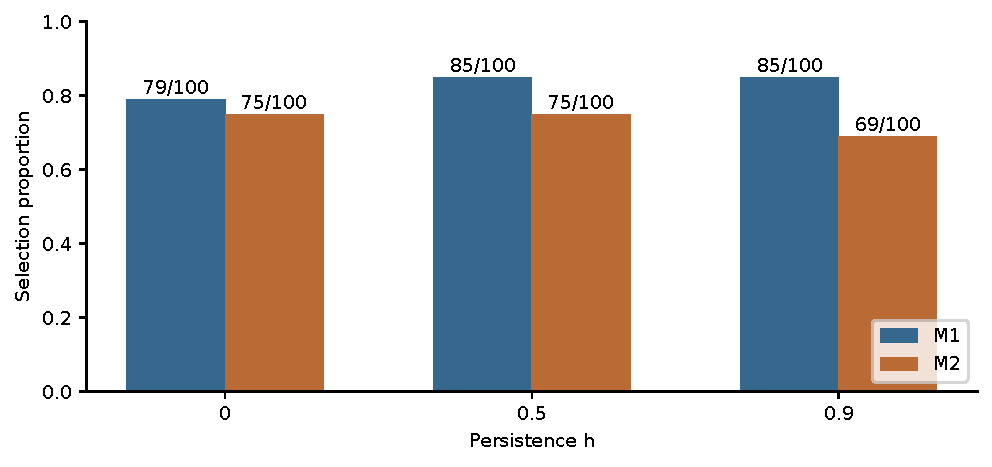
\includegraphics[width=\textwidth]{s02_completed_selection.pdf}\caption{Completed selection proportions under M1 and M2, each based on 100 paired forest units. The display is descriptive; saved custody checks and sampled raw validation passed.}\end{figure}


\part{Spatial Structure, Regional Transfer, Competitive Benchmarks, and Continuous Local Inhibition}
\chapter{Discrete Routing, Continuous Offspring Geography, and Background Nuisance in New Zealand}

In the tables, $I_{\mathrm{d,g}}$ denotes distance excitation with global stress (the saved identifier \texttt{I\_distance\_globalG}). A stacked mantissa and power of ten form one scientific-notation value; their full displayed precision is retained.
\label{ch:nz-spatial}
\section{From regional aggregation to matched spatial forecasts}
The successive studies below turn the locality question into matched predictive comparisons. They progress from three labelled zones (C1), through a conserved cross-zone mixing law (W), finite-cell distance allocation (D), and continuous-area offspring density (S), to a joint temporal--spatial/background factorial. These stages reuse the historical windows; their gains cannot be concatenated into an independent replication count. The regional algebra motivates the completed comparisons without identifying a geological mechanism.

\paragraph{Execution provenance.}
This chapter retains the original spatial and background-extension fits and numerical audits. The later selected-state replay recomputes the declared likelihoods using the recovered cached features and reconciles the common-space and partition comparisons. It does not rerun optimizer searches. The fresh frozen diagnostic and autonomous fits in Chapter~\ref{ch:observed} are separate computations.

The completed spatial programme compared, on the same region-labelled observations, three deliberately matched candidates: no inhibition, pooled inhibition across regions, and local inhibition. For a given regional history, the motivating schematic intensities are
\begin{align}
  \lambda_k^{(0)}&=B_k+H_k, \label{eq:locality-none}\\
  \lambda_k^{(\mathrm{pool})}
    &=B_k\exp\!\left(-\eta\sum_jG_j\right)+H_k, \label{eq:locality-pooled}\\
  \lambda_k^{(\mathrm{local})}
    &=B_k\exp(-\eta G_k)+H_k, \label{eq:locality-local}
\end{align}
where \(H_k\) includes the trigger amplitude and must be defined identically across alternatives. A fair comparison matches spatial backgrounds, triggering families with a serious Omori baseline, mark and history rules, observation rules, and fitting effort. With region label \(r_i\) for event \(i\), every candidate uses the same joint score
\begin{equation}
 \ell=\sum_i\log\lambda_{r_i}(t_i-)
      -\sum_k\int_0^T\lambda_k(t)\,\dif t
      +\sum_i\log f(m_i).
 \label{eq:proposed-spatial-score}
\end{equation}
The integrals include quiet regions and quiet intervals. Omitting them would reward or penalize models according to event allocation without accounting for exposure. Alternatively, candidates must be marginalized to the same label-discarded observations; a label-aware likelihood and a label-discarded likelihood cannot be ranked as if they used the same data event.


The subsequent stages declare their own background and geometry recipes. A later replay may differ at solver precision from an older sealed result; it does not replace that result. Throughout this chapter, an ``Event'' column is the point-event logsum contribution and ``Compensator'' is the signed contribution $C=-E$. For discrete zones/cells, the point intensity is with respect to counting measure; continuous comparisons below first put every arm on the same projected-area measure.

\section{C1: region-labelled local and global controls}

C1 supports localizing excitation for time-zone prediction, but does not support adding local stress inhibition to that localized excitation model. All three folds, four models, 12 case fits and 96 prescribed starts completed. The independent raw-row audit passed, reconciling 114 candidates and 96 solver returns; saved near-optimal forecasts passed the declared stability gate. The catalogue and historical authorities were preserved.

\subsection{Separate timing from zone prediction}

On the 612 held-out targets, local excitation beats global excitation by 349.786446 joint nats (+0.571546481 nats/event), positive in all three folds. Of this gain, 347.958257 nats comes from conditional-zone prediction and only 1.828190 nats from regional timing. Joint gains are +105.104546, +119.000978 and +125.680922 nats; timing differences are -2.083237, +1.797562 and +2.113864. The strong joint result therefore concerns predicting which of three fixed latitude bands receives the next event. It is not evidence of a comparably large improvement in event timing or of continuous-location forecast skill.

At the same parameters, local E0 and global E0 have exactly the same regional ground intensity and compensator. Their conditional-zone factors differ, so selecting each by full time-zone training NLL produces different fitted parameters and modestly different timing forecasts. The observed timing difference does not contradict the fixed-parameter identity.

Local inhibition also beats global inhibition strongly: +364.573096 joint nats (+0.595707674 nats/event), including +17.936860 regional-timing and +346.636237 conditional-zone nats. Both joint and timing differences are positive in all three folds. This comparison includes both localized triggering and localized stress, and the poor globally inhibited baseline. It does not establish the value of inhibition beyond a matched local excitation model.

\subsection{The matched inhibition result remains negative}

Adding local inhibition to local excitation loses 3.399761 joint nats (-0.005555164 nats/event): -2.077741 regional timing and -1.322020 conditional zone. Fold differences are -0.207862, -3.191896 and approximately zero (-0.000003) nats. The last difference is below the 0.0001-nat score-reconciliation tolerance and the selected eta is exactly zero; it should be described as a numerical tie rather than a substantive third forecast loss.

The local inhibitory fit lowers training NLL by approximately 0.112071, 1.061892 and zero nats in Folds 0-2, respectively, yet none yields a substantive held-out gain. These are modest training improvements of a nested bounded fitting procedure, not evidence for a nonzero physical depletion parameter.

Global inhibition loses 18.186411 nats (-0.029716357 nats/event). The difference of matched inhibition contrasts is therefore +14.786650 nats (+0.024161193 nats/event): localization makes the inhibitory penalty much less severe, while the local incremental inhibition contrast remains negative. This descriptive difference is positive in Folds 0 and 2, negative in Fold 1. It is not a causal difference-in-differences design.

\subsection{Fold 0 and proper exposure accounting}

Fold 0's global inhibitory contrast is -16.988735 nats, decomposed into -33.904743 event and +16.916008 compensator nats. The matched local inhibitory contrast is -0.207862 nats: -3.000762 event and +2.792900 compensator nats. Regional timing improves from a -16.988735 global inhibitory penalty to a -0.831697 local inhibitory penalty; the local conditional-zone contribution is +0.623835 nats.

The proper Fold 0 local inhibitory score differences by zone are +0.289381 south, -0.141682 central and -0.355561 north. Their sum gives -0.207862. Across all three folds, the matched local inhibitory differences are negative in each zone: -1.199738, -1.134201 and -1.065822 nats. These are full zone contrasts with their own valid integrated exposures, not event-only geographical summaries.

The large local-versus-global joint gains cannot be reduced to a positive event term everywhere. For example, Fold 0 local E0 has a negative central-zone event contrast (-2.324219 nats), offset by a +17.184730 compensator contribution, giving a +14.860511 central-zone total. Quiet exposure and all-zone compensators are essential to the result.

\subsection{Parameters and historical reconciliation}

The selected global eta values are 1.451113, 0.230849 and 0.116715; local eta values are 0.374699, 0.517222 and 0. Local eta is smaller in Folds 0 and 2 but larger in Fold 1. There is no uniform shrinkage result. Local and global stress histories also differ in scale and composition, so eta alone is not a directly comparable measure of physical stress strength. No selected coordinate hits a restrictive box boundary except the local eta=0 boundary in Fold 2.

The fresh global inhibitory contrasts reproduce Stage A's global raw contrasts to numerical precision: Fold 0 shifts by about 1e-11 nats, Fold 1 by +0.000013869 and Fold 2 by -0.000009878. Fixed-parameter global reduction was independently verified; these tiny separately optimized fit shifts are not failures of that identity. Historical Iteration28's -16.517557 Fold 0 contrast belongs to its own fitted/nuisance recipe and remains a separate authority.

The old five-degree cell crosswalk regroups event log-intensity ratios only. C1 defines three zone intensities, without a within-zone cell probability model; consequently cell compensators and cell full likelihoods are undefined. Proper zone compensators remain separate. Historical cell event penalties are retained with their source hashes and are not spliced into new denominators.

\subsection{Delimited conclusion}

The useful result is strong retrospective categorical-zone prediction from localized triggering, with a small mixed-sign timing benefit for local E0. Localizing the whole inhibitory procedure largely removes the catastrophic global inhibition penalty, but the matched local inhibitory extension still adds no held-out value. This supports retaining \modeltag{E0}{local} as the better of these declared local procedures; it does not demonstrate physical stress inhibition or identify a causal spatial mechanism.

The result applies to three predeclared latitude bands, omega=0, fixed r=0.7 and the retained ML law on one previously examined regional catalogue. Training-only pi and beta were frozen for test; observed history updated predictably. No event-iid confidence interval, Wilks boundary test, global-optimum certificate, new partition, kernel search, C2 or other model stage follows from this review.

Evidence: results/\allowbreak{}\allowbreak{}analysis/summary.json; methods/\allowbreak{}\allowbreak{}observed\_\allowbreak{}saved\_\allowbreak{}audit.json; results/\allowbreak{}\allowbreak{}analysis/historical\_\allowbreak{}reconciliation.json; results/\allowbreak{}\allowbreak{}analysis/cell\_\allowbreak{}event\_\allowbreak{}crosswalk.json; design/spatial\_\allowbreak{}zone\_\allowbreak{}counts.json; protocol\_\allowbreak{}observed\_\allowbreak{}v1.json. This interpretation introduces no numerical refit or pinned-source change.

\subsection{C1: complete audited comparisons}

All three folds, four models (12 case fits), and 96 prescribed starts are complete. The same 612 held-out targets are scored once per model. The interpretation in Section~\ref{sec:empirical-interpretation} applies.

\begingroup\scriptsize\setlength{\tabcolsep}{2pt}\renewcommand{\arraystretch}{1.18}
\begin{longtable}{@{}>{\raggedright\arraybackslash}p{0.1251\textwidth}>{\raggedright\arraybackslash}p{0.1251\textwidth}>{\raggedright\arraybackslash}p{0.1251\textwidth}>{\raggedright\arraybackslash}p{0.1251\textwidth}>{\raggedright\arraybackslash}p{0.1251\textwidth}>{\raggedright\arraybackslash}p{0.1251\textwidth}>{\raggedright\arraybackslash}p{0.1251\textwidth}@{}}
\toprule
{}Comparison & Regional timing & Conditional zone & Magnitude & Joint nats & Nats/event & Positive folds \\
\midrule\endfirsthead
\toprule
Comparison & Regional timing & Conditional zone & Magnitude & Joint nats & Nats/event & Positive folds \\
\midrule\endhead
\midrule\multicolumn{7}{r}{\emph{Continued on next page}}\\
\endfoot
\bottomrule\endlastfoot
{}\modeltag{E0}{local}\allowbreak{}-\allowbreak{}\modeltag{E0}{global} & 1.82819 & 347.958 & 0 & 349.786 & 0.571546 & 3/3 \\
{}\modeltag{I0}{local}\allowbreak{}-\allowbreak{}\modeltag{I0}{global} & 17.9369 & 346.636 & 0 & 364.573 & 0.595708 & 3/3 \\
{}\modeltag{I0}{local}\allowbreak{}-\allowbreak{}\modeltag{E0}{local} & -2.07774 & -1.32202 & 0 & -3.39976 & -0.00555516 & 0/3 \\
{}\modeltag{I0}{global}\allowbreak{}-\allowbreak{}\modeltag{E0}{global} & -18.1864 & \shortstack[r]{$-5.11591$\\$\times10^{-13}$} & 0 & -18.1864 & -0.0297164 & 0/3 \\
{}(\modeltag{I0}{local}\allowbreak{}-\allowbreak{}\modeltag{E0}{local})-(\modeltag{I0}{global}\allowbreak{}-\allowbreak{}\modeltag{E0}{global}) & 16.1087 & -1.32202 & 0 & 14.7866 & 0.0241612 & 2/3 \\
\end{longtable}\endgroup

% Audit-table relocation: app:audit10-c1
The complete C1 per-fold contrasts and exact zone decompositions are retained in Appendix~\ref{app:audit10-c1}.

\subsection{Scope}

K=3 fixed latitude zones, raw local stress, fixed ML excitation and r=.7, omega=0. Background proportions and magnitude nuisance use training only. Local triggering and local inhibition are compared with matched global/local excitation controls. Joint gains can come from zone prediction without improved regional timing; the two components must not be conflated.

The C1 model does not define within-zone cell probabilities, so cell event crosswalks have no invented cell compensators. Full compensator differences are reported per zone. Historical Iteration28 cell event penalties and recipe differences are retained separately in historical\_\allowbreak{}reconciliation.json.

All comparisons are retrospective on previously examined chronological windows. The common inferential and optimization boundaries in Section~\ref{sec:empirical-interpretation} apply. No follow-up model/kernel/productivity search or other stage was run.

\section{W: conserved cross-zone redistribution}

W supports a small training-estimated global redistribution component in the otherwise local excitation model for zone prediction. It does not support an incremental inhibitory extension or a direct timing benefit from the mixing weight. All 27 case fits and 216 prescribed starts completed; the independent raw-row audit passed, checking 279 candidates and 216 solver returns. Reported differences use 612 targets and common magnitude scores cancel.

\subsection{Excitation mixing improves the joint score through zone prediction}

Free-omega excitation improves on purely local excitation by 10.553372 joint nats (+0.017244071 nats/event), positive in all three held-out windows: +2.293398, +8.176718 and +0.083256 nats. Its conditional-zone gain is +13.789492 nats, while regional timing worsens by 3.236121 nats. Timing differences are +0.865688, -0.561462 and -3.540347 nats. The joint improvement should therefore be described as a categorical-zone forecast improvement with a net timing cost.

Selected excitation \(\omega\) values are 0.046125, 0.045172 and 0.044339. These are weights on a globally redistributed trigger component; they are not literal cross-zone offspring probabilities. The globally redistributed component can also return to the parent's own zone, so a parent's actual cross-zone allocation is \(\omega(1-\pi_{z_j})\), where \(z_j\) is the parent's zone. No physical transfer rate is identified by these fitted routing weights.

The free model's training NLL gains against omega0 are approximately 2.163997, 4.867366 and 13.271381 nats. Exact completed endpoint floors preserve the nested training comparison, and all prescribed starts and near-optimal forecast checks passed. Three similar estimates from overlapping training prefixes do not provide an independent replication or confidence interval for a physical mixing parameter.

Free excitation beats global excitation by 360.339778 joint nats (+0.588790487 nats/event), with +361.747747 conditional-zone nats and -1.407969 timing nats. This chiefly retains the large spatial prediction benefit already seen in C1, with an additional modest gain over the strictly local endpoint.

\subsection{Omega has no direct timing effect}

For either fixed stress choice and the same remaining parameters,

\begin{equation}\sum_z\lambda_z=\sum_z\pi_z e^{a+d x_{\mathrm{trend}}(t)-\eta G_z^{\rm stress}}+nH_{\rm global}.\end{equation}

Omega cancels because excitation allocation is column-stochastic. This holds for E and both local/global-stress I families. Ground likelihood and total compensator are omega-invariant at fixed (a,d,n,eta). The observed timing changes arise indirectly because full time-zone training refits those other coordinates. They do not overturn the shared-kernel timing-invariance result or establish direct improvement in event timing from cross-zone redistribution.

\subsection{Matched free inhibition remains negative}

With omega free in both matched models, local-stress inhibition loses 3.637297 joint nats (-0.005943296 nats/event) against excitation: -2.292422 timing and -1.344875 conditional-zone nats. Fold differences are +0.087297, -3.232617 and -0.491977 nats. Even the small Fold 0 joint gain combines worse timing (-0.704286) with better zone prediction (+0.791583). Regional timing is worse in all three windows.

Global-stress inhibition loses 12.887727 joint nats (-0.021058377 nats/event): -11.593479 timing and -1.294248 zone nats. Fold differences are -11.191948, +0.639379 and -2.335157 nats. Most of its aggregate loss remains in Fold 0. Local-stress inhibition outperforms global-stress inhibition in the free-omega comparison by 9.250429 nats, positive in two windows, but neither improves on matched excitation overall.

The selected free local-stress eta values are 0.281470, 0.579390 and 0.059749, with omega near 0.044-0.045. Free global-stress eta values are 0.910443, 0.133890 and 0.162321; their omega values are 0.068905, 0.048547 and 0.046997. These are fitted constrained prediction coordinates under different stress histories, not directly comparable physical stress strengths or a causal explanation of the losses.

\subsection{The factorial endpoints prevent a blanket localization claim}

At fixed local excitation (omega0), global-stress inhibition loses only 1.005026 aggregate nats, whereas local-stress inhibition loses 3.399764 nats. Thus local stress is not uniformly the better stress choice. The global-stress eta is 0.068165 in Fold 0 and exactly zero in Folds 1 and 2; its tiny positive score differences in those latter windows are numerical ties, not meaningful forecast wins.

At fixed global excitation (omega1), local-stress eta is exactly zero in all three windows. Its aggregate score difference from excitation is -0.000031725 nats, below the 0.0001-nat saved-score reconciliation tolerance, and should be treated as a nested numerical tie. Global-stress inhibition at that same excitation endpoint loses 18.186431 nats, including -16.988727 in Fold 0.

The factorial result is an interaction among excitation routing, stress choice and joint nuisance refitting. It does not justify a universal statement that localizing stress rescues inhibition. Much of the earlier local-versus-global improvement is attributable to excitation routing and conditional-zone forecasting. The raw positive-window counters in the audit retain arithmetic signs; eta0 differences of order1e-5 or1e-6 are not scientific evidence for an inhibitory gain.

\subsection{Proper exposure and conclusion}

All score contrasts include complete zone compensators. For example, Fold 0 free-local-inhibition versus free excitation has an event contribution of -2.002970 nats and a compensator contribution of +2.090266, giving +0.087297. Event penalties alone would give the wrong sign. No cell-within-zone score is present in this three-zone W stage; its full score is timing plus conditional zone plus common magnitude.

The delimited result favors free-omega excitation for categorical-zone forecasting among the declared W procedures, while the incremental local/global inhibitory alternatives remain negative overall. There is no direct omega timing effect, physical stress-transfer claim, event-iid confidence interval, Wilks boundary inference or global-optimum certificate.

D's model support, smoothing, distance grid, synthetic laws and selection rules were frozen before W outcomes. This interpretation changes none of them. Its historical admission depended on engineering correctness and protected resource/audit reserves; a positive W result was not an admission condition. The same held-out events were reused in D, rather than forming a fresh independent validation catalogue.

Evidence: results/\allowbreak{}\allowbreak{}W/analysis/\allowbreak{}\allowbreak{}summary.json; methods/\allowbreak{}\allowbreak{}W\_\allowbreak{}observed\_\allowbreak{}saved\_\allowbreak{}audit.json; protocol\_\allowbreak{}W\_\allowbreak{}observed.json; reports/\allowbreak{}\allowbreak{}W\_\allowbreak{}decision\_\allowbreak{}report.md. No new fit, source modification or extension was performed for this interpretation.

\subsection{W: complete audited comparisons}

All declared procedures and starts resolved. Source and audit bind this report to the frozen protocol. The interpretation in Section~\ref{sec:empirical-interpretation} applies.

\begingroup\scriptsize\setlength{\tabcolsep}{2pt}\renewcommand{\arraystretch}{1.18}
\begin{longtable}{@{}>{\raggedright\arraybackslash}p{0.1251\textwidth}>{\raggedright\arraybackslash}p{0.1251\textwidth}>{\raggedright\arraybackslash}p{0.1251\textwidth}>{\raggedright\arraybackslash}p{0.1251\textwidth}>{\raggedright\arraybackslash}p{0.1251\textwidth}>{\raggedright\arraybackslash}p{0.1251\textwidth}>{\raggedright\arraybackslash}p{0.1251\textwidth}@{}}
\toprule
{}Comparison & Regional timing & Conditional zone & Within-zone cell & Joint nats & Nats/event & Positive folds \\
\midrule\endfirsthead
\toprule
Comparison & Regional timing & Conditional zone & Within-zone cell & Joint nats & Nats/event & Positive folds \\
\midrule\endhead
\midrule\multicolumn{7}{r}{\emph{Continued on next page}}\\
\endfoot
\bottomrule\endlastfoot
{}\modeltag{E}{wfree}\allowbreak{}-\allowbreak{}\modeltag{E}{w0} & -3.23612 & 13.7895 & 0 & 10.5534 & 0.0172441 & 3/3 \\
{}\modeltag{E}{wfree}\allowbreak{}-\allowbreak{}\modeltag{E}{w1} & -1.40797 & 361.748 & 0 & 360.34 & 0.58879 & 3/3 \\
{}\modeltag{Ilocal}{wfree}\allowbreak{}-\allowbreak{}\modeltag{E}{wfree} & -2.29242 & -1.34487 & 0 & -3.6373 & -0.0059433 & 1/3 \\
{}\modeltag{Iglobal}{wfree}\allowbreak{}-\allowbreak{}\modeltag{E}{wfree} & -11.5935 & -1.29425 & 0 & -12.8877 & -0.0210584 & 1/3 \\
{}\modeltag{Ilocal}{w0}\allowbreak{}-\allowbreak{}\modeltag{E}{w0} & -2.07775 & -1.32201 & 0 & -3.39976 & -0.00555517 & 1/3 \\
{}\modeltag{Iglobal}{w0}\allowbreak{}-\allowbreak{}\modeltag{E}{w0} & -0.528304 & -0.476721 & 0 & -1.00503 & -0.0016422 & 2/3 \\
{}\modeltag{Ilocal}{w1}\allowbreak{}-\allowbreak{}\modeltag{E}{w1} & \shortstack[r]{$-3.17254$\\$\times10^{-5}$} & \shortstack[r]{$-1.7053$\\$\times10^{-13}$} & 0 & \shortstack[r]{$-3.17254$\\$\times10^{-5}$} & \shortstack[r]{$-5.18389$\\$\times10^{-8}$} & 0/3 \\
{}\modeltag{Iglobal}{w1}\allowbreak{}-\allowbreak{}\modeltag{E}{w1} & -18.1864 & \shortstack[r]{$-1.7053$\\$\times10^{-13}$} & 0 & -18.1864 & -0.0297164 & 0/3 \\
{}\modeltag{Ilocal}{wfree}\allowbreak{}-\allowbreak{}\modeltag{Iglobal}{wfree} & 9.30106 & -0.0506271 & 0 & 9.25043 & 0.0151151 & 2/3 \\
\end{longtable}\endgroup

% Audit-table relocation: app:audit10-w
The complete W window-level event/compensator contrasts and target-region exposures are retained in Appendix~\ref{app:audit10-w}.

\subsection{Routing interpretation}
Magnitude-score differences cancel because the mark forecast is shared. W estimates cross-zone redistribution and independently varies stress localization. Column-stochastic mixing preserves total triggering at fixed remaining parameters; a timing difference after joint refitting is indirect. The same previously inspected targets recur in D and the later density comparisons, so completed stage protocols do not make these independent replications.

\section{D: finite-distance cell allocation}

The fixed-cell distance excitation procedure improves categorical location forecasts on this catalogue, but not regional timing against its primary C 1-cell comparator. Adding either tested inhibitory extension remains negative in aggregate. All 33 D procedures (21 main fits and 12 scale selectors), 264 starts and the independent raw-row saved audit completed; the audit checked 312 candidates and 264 solver returns.

The primary \modeltag{E}{distance}\allowbreak{}-\allowbreak{}\modeltag{E}{bridge} gain is 74.843795 nats (+0.122293783 nats/event), positive in all three windows: +3.445007, +33.268354 and +38.130434. It decomposes into -3.259471 regional timing, -5.704315 conditional-zone and +83.807581 conditional-within-zone cell nats. The improvement concerns which of nine fixed cells receives an event. It is not a timing or continuous-location density gain. \modeltag{E}{bridge} is the strict omega 0 C 1 procedure refined onto the same cell space; it is not W's improved free-omega reference.

Training E selected sigma=150,150,50 km from the frozen four-point grid. The third choice reaches the grid's lower boundary. Cross-grid near-optimal forecast spreads were approximately 0.000002113, 0.000011607 and 0.000002524 nats/event, below the declared 0.01 gate. This establishes saved forecast stability under that criterion, not identification of a physical distance scale or an optimum beyond the grid. The global infinite-scale model remains a separate baseline, not a fifth selected point.

At the same background/productivity parameters, normalized excitation columns preserve the ground intensity for every E scale. The observed E timing differences after full-cell joint training are indirect consequences of refitting other parameters. Distance inhibition can additionally change timing through its unnormalized stress similarity, which is distinct from the normalized triggering probability. Its stress scale was tied to the E-selected scale; no separate stress-range search occurred.

\modeltag{I}{distance}\allowbreak{}-\allowbreak{}\modeltag{E}{distance} is -2.275081 nats (-0.003717452 nats/event), comprising -0.516136 timing, -6.109160 zone and +4.350215 within-zone cell nats. Two windows gain (+0.452200 and +0.013479), but the middle window loses 2.740760 nats and determines the negative aggregate. Positive-window counts do not replace the event-weighted total. The global-stress alternative loses 2.990767 nats; local distance stress improves on that alternative by 0.715686 nats but neither beats matched excitation overall.

The local distance eta estimate equals its upper bound 3 in ALL THREE folds. Its training NLL gains against E are approximately 2.025365,5.832549 and 1.033420 nats, yet aggregate held-out performance is negative. These are bound-limited results for the declared procedure. They do not establish an unconstrained eta optimum, absence of physical stress effects, or performance under a larger bound or different independently selected stress range. No bound expansion or refit was performed.

All nine cells remain supported by predeclared hierarchical half-count smoothing, which preserves the original training zone proportions. This includes the held-out event in a previously unoccupied training cell. Proper compensators cover every target cell, including quiet/unoccupied cells. Unlike the old C 1 event-only cell crosswalk, D explicitly supplies cell intensities, so its cell P+C contrasts are defined. The new C 1-cell bridge is a declared q allocation, not a retroactive alteration of historical C 1 scores.

The separately labeled secondary comparison refines fixed W \modeltag{E}{wfree} to this same cell space without refitting. \modeltag{E}{distance} gains 64.290424 nats (+0.105049712 nats/event), positive in all three windows; its timing difference is -0.023350, zone difference -19.493808 and within-zone cell gain +83.807581 nats. This supports an additional categorical-within-zone benefit even against the improved W reference, while providing no net timing improvement. It remains adaptive reporting, planned after W and before opening D outcomes, rather than an original primary contrast or independent validation.

Scope: fixed ML/r=.7, nine categorical cells, the predeclared four-scale grid and eta bound, one previously examined catalogue and reused chronological targets. No continuous spatial-density validation, physical causality, event-iid interval, Wilks boundary claim, global optimum certificate or further search follows. Evidence is in the D analysis/audit tables and the separately audited secondary common-space outputs.

\subsection{D: complete audited comparisons}

All declared procedures and starts resolved. Source and audit bind this report to the frozen protocol. The interpretation in Section~\ref{sec:empirical-interpretation} applies.

\begingroup\scriptsize\setlength{\tabcolsep}{2pt}\renewcommand{\arraystretch}{1.18}
\begin{longtable}{@{}>{\raggedright\arraybackslash}p{0.1251\textwidth}>{\raggedright\arraybackslash}p{0.1251\textwidth}>{\raggedright\arraybackslash}p{0.1251\textwidth}>{\raggedright\arraybackslash}p{0.1251\textwidth}>{\raggedright\arraybackslash}p{0.1251\textwidth}>{\raggedright\arraybackslash}p{0.1251\textwidth}>{\raggedright\arraybackslash}p{0.1251\textwidth}@{}}
\toprule
{}Comparison & Regional timing & Conditional zone & Within-zone cell & Joint nats & Nats/event & Positive folds \\
\midrule\endfirsthead
\toprule
Comparison & Regional timing & Conditional zone & Within-zone cell & Joint nats & Nats/event & Positive folds \\
\midrule\endhead
\midrule\multicolumn{7}{r}{\emph{Continued on next page}}\\
\endfoot
\bottomrule\endlastfoot
{}\modeltag{E}{bridge}\allowbreak{}-\allowbreak{}\modeltag{E}{global} & 1.82817 & 347.958 & \shortstack[r]{$1.42109$\\$\times10^{-14}$} & 349.786 & 0.571546 & 3/3 \\
{}\modeltag{I}{bridge}\allowbreak{}-\allowbreak{}\modeltag{I}{global} & 17.9368 & 346.636 & \shortstack[r]{$-2.13163$\\$\times10^{-13}$} & 364.573 & 0.595708 & 3/3 \\
{}\modeltag{I}{bridge}\allowbreak{}-\allowbreak{}\modeltag{E}{bridge} & -2.07775 & -1.32201 & \shortstack[r]{$2.84217$\\$\times10^{-14}$} & -3.39976 & -0.00555517 & 1/3 \\
{}\modeltag{E}{distance}\allowbreak{}-\allowbreak{}\modeltag{E}{bridge} & -3.25947 & -5.70432 & 83.8076 & 74.8438 & 0.122294 & 3/3 \\
{}\modeltag{E}{distance}\allowbreak{}-\allowbreak{}\modeltag{E}{global} & -1.4313 & 342.254 & 83.8076 & 424.63 & 0.69384 & 3/3 \\
{}\modeltag{I}{distance}\allowbreak{}-\allowbreak{}\modeltag{E}{distance} & -0.516136 & -6.10916 & 4.35022 & -2.27508 & -0.00371745 & 2/3 \\
{}\modeltag{I}{d,g}-\modeltag{E}{distance} & -2.85336 & 0.0832518 & -0.220656 & -2.99077 & -0.00488687 & 1/3 \\
{}\modeltag{I}{distance}\allowbreak{}-\allowbreak{}\modeltag{I}{d,g} & 2.33723 & -6.19241 & 4.57087 & 0.715686 & 0.00116942 & 2/3 \\
\end{longtable}\endgroup

% Audit-table relocation: app:audit10-d
The complete D window-level contrasts and target-cell exposures are retained in Appendix~\ref{app:audit10-d}.



\subsection{Common-observation reconciliation}

Secondary/adaptive reporting after W, planned before opening D outcomes; not an original primary contrast or a new fit. These contrasts are descriptive; no confidence intervals are supplied.

The reference is the fixed audited W \modeltag{E}{wfree} forecast, refined to nine cells with the already frozen training q(c|z). Timing and conditional-zone scores remain unchanged; the within-zone cell term is sum log q and each cell compensator is q times its W zone compensator. All seven D main models are compared without refitting or reselection.

\begingroup\scriptsize\setlength{\tabcolsep}{2pt}\renewcommand{\arraystretch}{1.18}
\begin{longtable}{@{}>{\raggedright\arraybackslash}p{0.1080\textwidth}>{\raggedright\arraybackslash}p{0.1080\textwidth}>{\raggedright\arraybackslash}p{0.1080\textwidth}>{\raggedright\arraybackslash}p{0.1080\textwidth}>{\raggedright\arraybackslash}p{0.1080\textwidth}>{\raggedright\arraybackslash}p{0.1080\textwidth}>{\raggedright\arraybackslash}p{0.1080\textwidth}>{\raggedright\arraybackslash}p{0.1080\textwidth}@{}}
\toprule
{}D candidate minus refined W reference & Timing & Zone & Within-zone cell & Magnitude & Joint nats & Nats/event & Positive folds \\
\midrule\endfirsthead
\toprule
D candidate minus refined W reference & Timing & Zone & Within-zone cell & Magnitude & Joint nats & Nats/event & Positive folds \\
\midrule\endhead
\midrule\multicolumn{8}{r}{\emph{Continued on next page}}\\
\endfoot
\bottomrule\endlastfoot
{}\modeltag{E}{global} & 1.40795 & -361.748 & \shortstack[r]{$1.42109$\\$\times10^{-14}$} & 0 & -360.34 & -0.588791 & 0/3 \\
{}\modeltag{I}{global} & -16.7785 & -361.748 & 0 & 0 & -378.526 & -0.618507 & 0/3 \\
{}\modeltag{E}{bridge} & 3.23612 & -13.7895 & \shortstack[r]{$1.42109$\\$\times10^{-14}$} & 0 & -10.5534 & -0.0172441 & 0/3 \\
{}\modeltag{I}{bridge} & 1.15837 & -15.1115 & 0 & 0 & -13.9531 & -0.0227992 & 0/3 \\
{}\modeltag{E}{distance} & -0.02335 & -19.4938 & 83.8076 & 0 & 64.2904 & 0.10505 & 3/3 \\
{}\modeltag{I}{distance} & -0.539486 & -25.603 & 88.1578 & 0 & 62.0153 & 0.101332 & 3/3 \\
{}\modeltag{I}{d,g} & -2.87671 & -19.4106 & 83.5869 & 0 & 61.2997 & 0.100163 & 2/3 \\
\end{longtable}\endgroup

% Audit-table relocation: app:audit10-common
The complete window arithmetic for the secondary common-space comparison, together with its reconciliation scope, is retained in Appendix~\ref{app:audit10-common}.

\subsection{Shared limits of the W and D comparisons}
W and D completed 60 observed procedures, 480 mandatory starts and 591 audited observed candidates; their fixed-seed engineering schedules completed 40 procedures and 320 starts. The secondary common-space comparison retained all 21 per-window contrasts and seven aggregates without refitting. Its refinement preserves the W timing and zone scores, adds the fixed conditional-cell allocation, and supplies corresponding cell compensators.
The distance excitation gains against refined W are +1.151609, +25.091636 and +38.047178 nats by window. Its aggregate timing difference is small in score units but is not a formal equivalence result. The two distance inhibitory models also beat refined W by +62.015343 and +61.299657 nats, while both remain below matched distance excitation. Beating a coarser reference therefore does not establish incremental inhibition.
The scientific scope is coarse spatial allocation under declared grids and bounds. Normalized routing does not directly change regional intensity at fixed parameters, selected ranges do not identify physical interaction distances, and no event-iid interval, global optimum or causal mechanism follows. Detailed contrasts, parameters and exposures are retained in Appendix~\ref{app:audit10}.

\section{S: continuous area density}

Continuous-area triggering substantially improved held-out point-location density forecasts relative to the projected cell-center lift, but did not improve regional event timing. Across the same 612 targets, \modeltag{E}{cont} minus \modeltag{E}{lift} gained 1,458.803884 joint nats (+2.383666477 nats/event), while losing 10.470041 timing nats. Most of the joint gain came from resolving locations within cells. Neither the zone-stress nor global-stress inhibitory extension supplied a meaningful incremental forecast gain.

This is principally a check of spatial discretization: a continuous density is compared with uniform spreading of cell mass, not with an equally resolved competitive spatial model. The +1,452.412080 within-cell nats account for almost all of the joint gain. The score improvement is real for these declared forecast distributions and common units, but its size does not establish a new physical mechanism or superiority over a strong continuous benchmark. The earlier national-routing reference is likewise a coarse spatial ablation.

All 42 planned procedures and 336 prescribed starts completed. The two selected E models per fold are aliases of existing selector results, not extra fits. The independent raw-row audit replayed 384 candidates and 336 solver returns, reconstructed geometry and positive rectangle integrals independently, and found stable candidate forecasts. The score contrasts below are descriptive, without confidence intervals.

\begingroup\scriptsize\setlength{\tabcolsep}{2pt}\renewcommand{\arraystretch}{1.18}
\begin{longtable}{@{}>{\raggedright\arraybackslash}p{0.1480\textwidth}>{\raggedright\arraybackslash}p{0.1480\textwidth}>{\raggedright\arraybackslash}p{0.1480\textwidth}>{\raggedright\arraybackslash}p{0.1480\textwidth}>{\raggedright\arraybackslash}p{0.1480\textwidth}>{\raggedright\arraybackslash}p{0.1480\textwidth}@{}}
\toprule
{}Contrast & Fold 0 (203) & Fold 1 (155) & Fold 2 (254) & Total joint nats & Nats/event \\
\midrule\endfirsthead
\toprule
Contrast & Fold 0 (203) & Fold 1 (155) & Fold 2 (254) & Total joint nats & Nats/event \\
\midrule\endhead
\midrule\multicolumn{6}{r}{\emph{Continued on next page}}\\
\endfoot
\bottomrule\endlastfoot
{}\modeltag{E}{cont}\allowbreak{}-\allowbreak{}\modeltag{E}{lift} & +549.866921 & +457.463557 & +451.473406 & +1458.803884 & +2.383666477 \\
{}\modeltag{E}{cont}\allowbreak{}-\allowbreak{}E\_\allowbreak{}oldD\_\allowbreak{}lift & +549.307187 & +462.729938 & +451.046777 & +1463.083902 & +2.390659970 \\
{}\modeltag{E}{cont}\allowbreak{}-\allowbreak{}\modeltag{E}{global} & +657.856745 & +614.999257 & +614.858124 & +1887.714125 & +3.084500205 \\
{}I\_\allowbreak{}cont\_\allowbreak{}zone-\modeltag{E}{cont} & +0.000032 & -0.211419 & -0.186526 & -0.397913 & -0.000650184 \\
{}I\_\allowbreak{}cont\_\allowbreak{}globalG-\modeltag{E}{cont} & +0.000032 & -0.000016 & -0.000004 & +0.000013 & +0.000000021 \\
{}\modeltag{E}{lift}\allowbreak{}-\allowbreak{}E\_\allowbreak{}oldD\_\allowbreak{}lift & -0.559734 & +5.266381 & -0.426630 & +4.280018 & +0.006993493 \\
\end{longtable}\endgroup

The continuous model wins joint point scores in all three windows against each excitatory comparator. Against \modeltag{E}{lift}, its timing differences are -3.163215, +0.705482 and -8.012308 nats; it improves timing in only Fold 1. The aggregate joint decomposition is:

\begingroup\small\setlength{\tabcolsep}{2pt}\renewcommand{\arraystretch}{1.18}
\begin{longtable}{@{}>{\raggedright\arraybackslash}p{0.4680\textwidth}>{\raggedright\arraybackslash}p{0.4680\textwidth}@{}}
\toprule
{}Component, \modeltag{E}{cont} minus \modeltag{E}{lift} & Nats \\
\midrule\endfirsthead
\toprule
Component, \modeltag{E}{cont} minus \modeltag{E}{lift} & Nats \\
\midrule\endhead
\midrule\multicolumn{2}{r}{\emph{Continued on next page}}\\
\endfoot
\bottomrule\endlastfoot
{}Regional timing & -10.470041 \\
{}Conditional zone & -4.471988 \\
{}Conditional cell within zone & +21.333833 \\
{}Within-cell area logdensity & +1452.412080 \\
{}Magnitude & 0.000000 \\
{}Joint & +1458.803884 \\
\end{longtable}\endgroup

The corresponding point-event contribution is +1448.297321 nats and compensator contribution +10.506563, which reconcile to the joint gain because the common magnitude term cancels. This is evidence of improved conditional location prediction, predominantly inside the original coarse cells. It must not be reported as a 1,458.8-nat improvement in event timing. Normalized spatial triggering leaves the regional ground intensity unchanged at fixed nuisance parameters; the smaller timing differences arise through refitting those nuisance parameters to joint point likelihood.

Both families use actual unsnapped parent coordinates and the same equal-area projection, background density, six-point scale grid and square-kilometre area measure. The continuous model evaluates actual target points and analytically integrates each parent kernel over the rectangular domain. \modeltag{E}{lift} allocates parent mass at projected target-cell centers and spreads that mass uniformly within a cell. Its within-cell density is therefore fixed by cell area, whereas \modeltag{E}{cont} predicts subcell locations. The decomposition is proper: the within-cell term is an area logdensity, not a discrete probability.

\begingroup\footnotesize\setlength{\tabcolsep}{2pt}\renewcommand{\arraystretch}{1.18}
\begin{longtable}{@{}>{\raggedright\arraybackslash}p{0.1800\textwidth}>{\raggedright\arraybackslash}p{0.1800\textwidth}>{\raggedright\arraybackslash}p{0.1800\textwidth}>{\raggedright\arraybackslash}p{0.1800\textwidth}>{\raggedright\arraybackslash}p{0.1800\textwidth}@{}}
\toprule
{}Fold & \modeltag{E}{cont} selected sigma (km) & \modeltag{E}{lift} selected sigma (km) & Zone-I eta & Global-I eta \\
\midrule\endfirsthead
\toprule
Fold & \modeltag{E}{cont} selected sigma (km) & \modeltag{E}{lift} selected sigma (km) & Zone-I eta & Global-I eta \\
\midrule\endhead
\midrule\multicolumn{5}{r}{\emph{Continued on next page}}\\
\endfoot
\bottomrule\endlastfoot
{}0 & 5 & 150 & 0.000000000 & 0.000000000 \\
{}1 & 15 & 150 & 0.068954189 & 0.000000000 \\
{}2 & 15 & 5 & 0.021703682 & 0.000000000 \\
\end{longtable}\endgroup

The continuous scale is at the 5-km lower grid boundary in Fold 0 and at 15 km in Folds 1 and 2. The data and this finite grid do not identify a universal physical interaction length or support extrapolation below 5 km. Each family selects its own scale using training likelihood; \modeltag{E}{cont} versus \modeltag{E}{lift} is a comparison of complete selection procedures, rather than a fixed-scale-only geometric effect. The small near-optimal forecast spreads certify local forecast stability under the prescribed candidate pool, not unique identification of sigma.

Zone inhibition selects eta=0 in Fold 0 and small positive eta in Folds 1 and 2. Its aggregate change is -0.397913 joint nats (-0.000650184 per event), including -0.115282 timing nats. Fold 0 differs from E only by approximately 0.000032 nats at eta=0, a solver-scale tie; the other windows lose 0.211419 and 0.186526 nats. Global inhibition selects eta=0 in every fold. Its aggregate +0.000013 nats is below the 0.0001-nat reconciliation tolerance and is a numerical tie, not evidence of benefit. Both inhibition procedures use the same \modeltag{E}{cont}\allowbreak{}-\allowbreak{}selected sigma without reselection. Stress remains a raw three-zone or global temporal field, not a continuously resolved spatial stress field.

The sealed old C \modeltag{E}{distance} and \modeltag{E}{global} references were not refitted. They were lifted to point densities by dividing cell intensity by the exact projected cell area; their categorical joint totals subtract the same sum of test log-cell-areas. The independently checked lift identity puts every displayed contrast on the same \(\mathrm{km}^{-2}\) measure. \modeltag{E}{cont} gains 1,463.083902 nats over the old distance lift. The new \modeltag{E}{lift} gains only 4.280018 aggregate nats over that reference, winning one window. That latter contrast changes projection/target-center geometry, scale-grid range and fresh fitting, so it is not a pure metric effect. Neither comparison directly subtracts categorical and density likelihoods.

Two harness failures were retained and repaired in append-only epochs. First, six historical fit-file identity pins were missing although their identical model contents were already inside pinned old case JSON. The 14 completed first-case procedures and 112 starts were reused; only the remaining 28 procedures and 224 starts were newly run. Second, the independent old-anchor oracle recorded a unit diagnostic normalizer instead of the raw pi-weighted kernel sum. One diagnostic assignment was repaired; normalized masses, densities, likelihoods, gradients, fits, scores and tolerances were unchanged. A complete recovery-aware raw-row audit then passed. No completed start was refitted and no synthetic history was redrawn. Failed-attempt and audit wall time remain charged in final accounting.

This is retrospective evidence on a previously inspected catalogue and fixed finite domain. Isotropy is Euclidean in the declared cylindrical equal-area projection, not geodesic equivalence. The background remains nine-cell piecewise density, temporal excitation is fixed unit-scale ML with r=0.7, and no joint O/S model was fit. There are no event-iid intervals, Wilks boundary claims, physical-causality conclusions or universal bandwidth claims. The appropriate scientific conclusion is a strong location-density improvement for this continuous triggering procedure, with no accompanying timing improvement and no meaningful incremental inhibition gain.

Exact score and boundary tables are in summary.json, with the terminal independent reconciliation in observed\_\allowbreak{}saved\_\allowbreak{}audit\_\allowbreak{}v3.json.

\section{Joint temporal--spatial and background comparison}

A matched comparison of twelve earthquake forecasting models finds positive predictive evidence from continuous event locations and, within that representation, Omori temporal decay. The experiment reuses 612 historical targets across three chronological windows. A training-only kernel-density background reduces but does not remove the continuous-location advantage over a cell approximation: gains remain 2.326-2.369 nats per event across three temporal families. With that stronger background and continuous locations, Omori improves on fixed-scale Mittag-Leffler (ML) triggering by 15.474 joint-score nats, including 10.368 timing nats, with both components positive in every window. The fully combined procedure improves aggregate timing and location scores over its current matched coarse comparator; location prediction accounts for most of the gain. Negative temporal contrasts and losing 1-2 km sensitivity fits limit the interpretation. These are retrospective fitted-procedure comparisons, not independent confirmation, identification of physical triggering, or evidence for inhibition.

\section{Relation to the temporal and mark comparisons}

Chapter~\ref{ch:temporal-extensions} reports negative exploratory results from shared-kernel magnitude-class history and free productivity estimation. This chapter asks whether temporal decay and finer spatial representation improve forecasts after a more flexible background geography is supplied. These comparisons retain the earlier matched results and restricted theoretical conclusions. The withdrawn background-nuisance continuation remains a separate historical study.

The original discussion proposed that a spatial conditional intensity should be examined with common observations, proper compensators and serious temporal benchmarks. Subsequent research explored those directions. This chapter reports the jointly fitted temporal-spatial/background experiment, rather than attempting to concatenate gains from separate historical runs. Its key contribution is a controlled comparison showing that the location improvement persists under a stronger background, while the temporal benefit depends on the spatial representation and comparator.

The Hawkes/ETAS and fractional-triggering literature already cited in the manuscript bibliography supplies the modelling context. No novelty or reproduction claim for those model families is made here.

The authority is the sealed run \nolinkurl{temporal_spatial_background_20261024T211225Z}, source commit \nolinkurl{764f7e74576d71a3bd224990aa00491a533c13de}. The original sealed manuscript and addenda remain historical source authorities for this unified account. The decision report and complete audited summary provide the full comparison roster.

\section{Matched design and scoring}

The local GeoNet snapshot contains 913 events of magnitude at least 5.0. Training prefixes contain 301, 504 and 659 events; their disjoint test windows contain 203, 155 and 254 targets. Times are days since 1960-01-01 UTC, with horizon 24,394 days. All earlier observed events remain eligible parents. During a test window the forecast history updates with earlier observed test events, while fitted parameters and spatial nuisance estimates remain frozen. This is sequential conditional forecasting, not a single forecast of an entire future catalogue at the training cutoff.

The factorial crosses three temporal forms (fixed-scale ML, common free-scale ML, Omori), two immigrant-background representations (cell and KDE-enriched), and two offspring-location representations (continuous and cell-lift). All share fixed magnitude productivity parameter r = 0.7 and the same training-only conditional-bin magnitude-rate estimate. No new magnitude-productivity search is included.

For time t and projected location z, the conditional intensity has the form

\begin{align}
\lambda(t,z)&=e^{a+dx_{\mathrm{trend}}(t)}b_{\rm bg}(z)+n\sum_{j:t_j<t}\kappa_j k_\theta(t-t_j)s_\sigma(z\mid z_j),\\
x_{\mathrm{trend}}(t)&=2t/24394-1.
\end{align}

Here \(\kappa_j\) is the shared, training-calibrated magnitude-productivity weight of parent \(j\). Both spatial densities integrate to one over the fixed nine-cell domain. Consequently the integrated regional rate is the background amplitude plus the normalized temporal offspring contribution. The joint marked log score includes point-event log intensity, the full space-time compensator and the common magnitude density. It decomposes exactly into timing, conditional zone, conditional cell, within-cell area density and magnitude terms. Higher score is better. All location scores use the same projected-area measure in square kilometres; a joint gain is not a percentage improvement in accuracy.

Continuous offspring density is proportional to a fixed training-derived reference density times the radial factor (1 + squared distance / sigma squared) to power -2, normalized separately for each actual parent. The lift comparator uses target-cell-centre weights and spreads each resulting cell mass uniformly inside that cell; it also retains actual parent coordinates. The radial factor is isotropic in the declared equal-area projection, but reference weighting and domain truncation make the full density generally anisotropic and piecewise smooth.

Where the fixed nine-cell reference density changes across a cell boundary, multiplication by that density can give the offspring density a step discontinuity even though the radial factor is smooth. Normalization preserves its unit mass but does not remove those artificial grid-boundary jumps. This limits any interpretation as a smooth physical stress or transport field.

The KDE-enriched background mixes 95\% training kernel density with a fixed 5\% cell-density floor. Each kernel is separately normalized on the finite domain. Bandwidth selection uses spatial leave-one-out scores, removing exactly the scored row from both density and hierarchical counts. After selection the full-training plug-in density, including self-kernels, is frozen. It estimates observed event geography, not an identified immigrant distribution; in-sample fitting therefore includes nuisance reuse.

This undeclustered plug-in background uses all training events, including events generated by triggering. It therefore mixes background and clustered seismicity; leave-one-out bandwidth selection does not turn it into an identified immigrant density. Stochastic declustering instead estimates background and triggering contributions jointly or probabilistically \citep{ZhuangOgataVereJones2002}. The retained self-kernels can increase in-sample density at training coordinates, a nuisance-fitting limitation rather than test-location inclusion.

Fixed ML uses the pinned normalized 195-mode mixture at one day. Common ML estimates its scale over 0.001-20 days; Omori estimates c over 0.0001-20 days and p over 1.01-2.5. Temporal kernels have unit mass over all positive lags, with exact finite-window exposure rather than window renormalization. Spatial scale sigma is selected once per fold by the fixed-ML/cell-background/continuous baseline from 5, 15, 50, 150, 500 and 1500 km, then shared across all twelve primary procedures. Free parameters are refitted separately within each procedure. These are conditional shared-scale comparisons, not independent spatial optimization for every model. The frozen protocol specifies bounds, starts and selection rules.

\section{Temporal improvement is positive but conditional}

The table below reports continuous-location comparisons. Differences are candidate minus reference, aggregated over the same 612 targets; nats/event is total gain divided by 612. These contrasts are descriptive; no confidence intervals are supplied.

\begingroup\footnotesize\setlength{\tabcolsep}{2pt}\renewcommand{\arraystretch}{1.18}
\begin{longtable}{@{}>{\raggedright\arraybackslash}p{0.1800\textwidth}>{\raggedright\arraybackslash}p{0.1800\textwidth}>{\raggedright\arraybackslash}p{0.1800\textwidth}>{\raggedright\arraybackslash}p{0.1800\textwidth}>{\raggedright\arraybackslash}p{0.1800\textwidth}@{}}
\toprule
{}Background and temporal contrast & Joint nats & Nats/event & Timing nats & Joint-positive windows \\
\midrule\endfirsthead
\toprule
Background and temporal contrast & Joint nats & Nats/event & Timing nats & Joint-positive windows \\
\midrule\endhead
\midrule\multicolumn{5}{r}{\emph{Continued on next page}}\\
\endfoot
\bottomrule\endlastfoot
{}Cell: common ML - fixed ML & -1.25 & -0.00204249 & +1.4546 & 2/3 \\
{}Cell: Omori - fixed ML & +67.9659 & +0.111055 & +23.4194 & 3/3 \\
{}Cell: Omori - common ML & +69.2159 & +0.113098 & +21.9648 & 3/3 \\
{}KDE-enriched: common ML - fixed ML & +5.61686 & +0.00917788 & +9.6524 & 2/3 \\
{}KDE-enriched: Omori - fixed ML & +15.4742 & +0.0252847 & +10.3682 & 3/3 \\
{}KDE-enriched: Omori - common ML & +9.85737 & +0.0161068 & +0.715779 & 1/3 \\
\end{longtable}\endgroup

With the KDE-enriched background, Omori's joint gains over fixed ML are +0.687236, +0.845910 and +13.941085 nats; timing gains are +3.042197, +2.293691 and +5.032289. The timing improvement therefore survives the stronger background in each window, although most joint gain occurs in the third.

The comparison against common-scale ML is less consistent: joint differences are -1.091786, -5.559124 and +16.508279 nats. Moreover, under KDE-enriched background and cell-lift geography, Omori loses 10.186077 joint nats and 0.970870 timing nats to fixed ML. The evidence favours Omori over fixed ML within the continuous representation, not universal superiority of one kernel.

\begin{figure}[htbp]\centering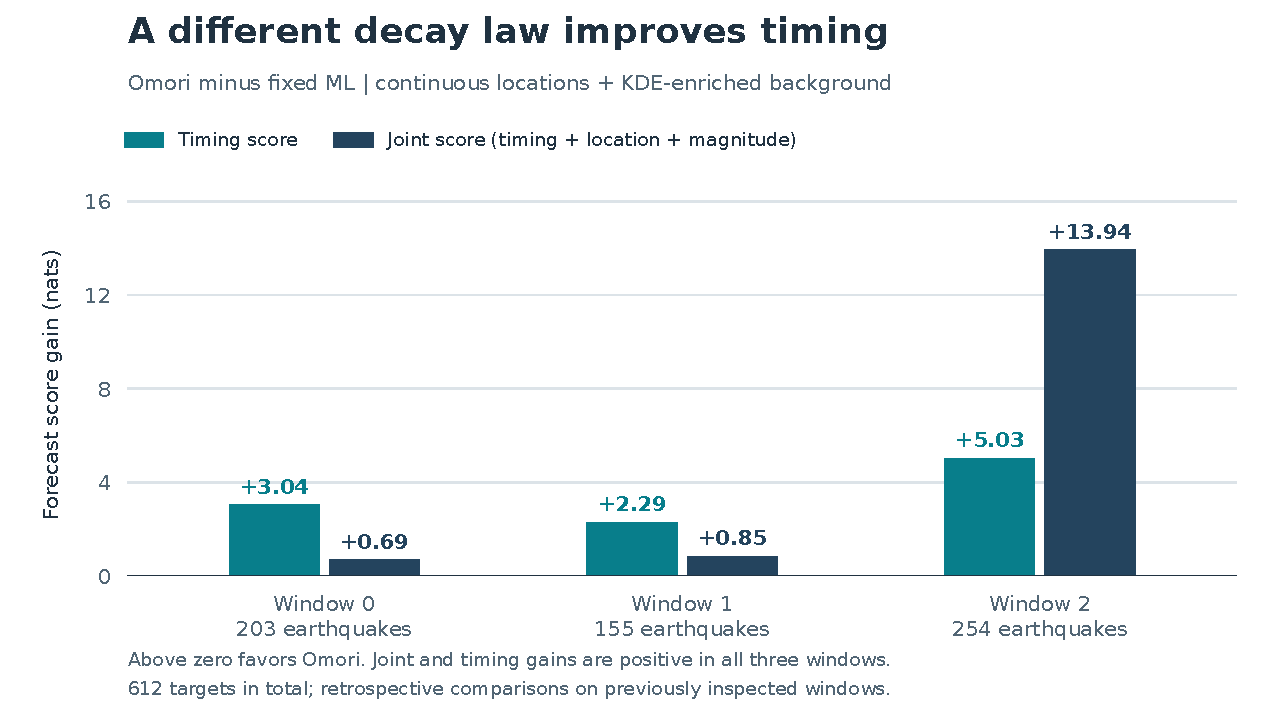
\includegraphics[width=\linewidth,height=.78\textheight,keepaspectratio]{spatial_addendum_iii_fig1_temporal.pdf}
\caption{Temporal comparisons across the three historical evaluation windows.}\end{figure}

\section{The location improvement survives stronger background geography}

Every continuous-minus-lift joint contrast wins all three windows under both backgrounds. The table below separates the spatial refinement from the effect of improving background geography. These contrasts are descriptive; no confidence intervals are supplied.

\begingroup\footnotesize\setlength{\tabcolsep}{2pt}\renewcommand{\arraystretch}{1.18}
\begin{longtable}{@{}>{\raggedright\arraybackslash}p{0.1800\textwidth}>{\raggedright\arraybackslash}p{0.1800\textwidth}>{\raggedright\arraybackslash}p{0.1800\textwidth}>{\raggedright\arraybackslash}p{0.1800\textwidth}>{\raggedright\arraybackslash}p{0.1800\textwidth}@{}}
\toprule
{}Temporal family & Continuous - lift, cell background (nats) & Continuous - lift, KDE-enriched background (nats) & KDE continuous--lift joint (nats/event) & KDE continuous--lift timing (nats) \\
\midrule\endfirsthead
\toprule
Temporal family & Continuous - lift, cell background (nats) & Continuous - lift, KDE-enriched background (nats) & KDE continuous--lift joint (nats/event) & KDE continuous--lift timing (nats) \\
\midrule\endhead
\midrule\multicolumn{5}{r}{\emph{Continued on next page}}\\
\endfoot
\bottomrule\endlastfoot
{}Fixed ML & +1453.29 & +1424.12 & +2.327 & +16.5456 \\
{}Common ML & +1445.7 & +1423.3 & +2.32565 & +15.1151 \\
{}Omori & +1507.21 & +1449.79 & +2.36893 & +27.8846 \\
\end{longtable}\endgroup

The stronger background reduces the continuous-location advantage by 22.397419-57.420970 nats. It explains some of that advantage, but does not remove it within the declared models.

Location dominates the remaining improvement. For Omori with KDE-enriched background, the +1449.785291 joint nats comprise +27.884617 timing, +14.810114 conditional-zone, +18.815997 conditional-cell and +1388.274563 within-cell area-density nats. Magnitude differences are zero. The timing aggregate is positive despite two losing windows (+35.932611, -2.308009, -5.739984); this spatial result must not be presented as uniform timing success.

Changing background geography itself improves continuous-model joint scores by 85.740055, 92.606919 and 33.248405 nats for fixed ML, common ML and Omori. For Omori that background change loses 1.757274 timing nats. At fixed common parameters, normalized spatial changes leave total regional intensity unchanged; their fitted timing effects arise through refitting.

\begin{figure}[htbp]\centering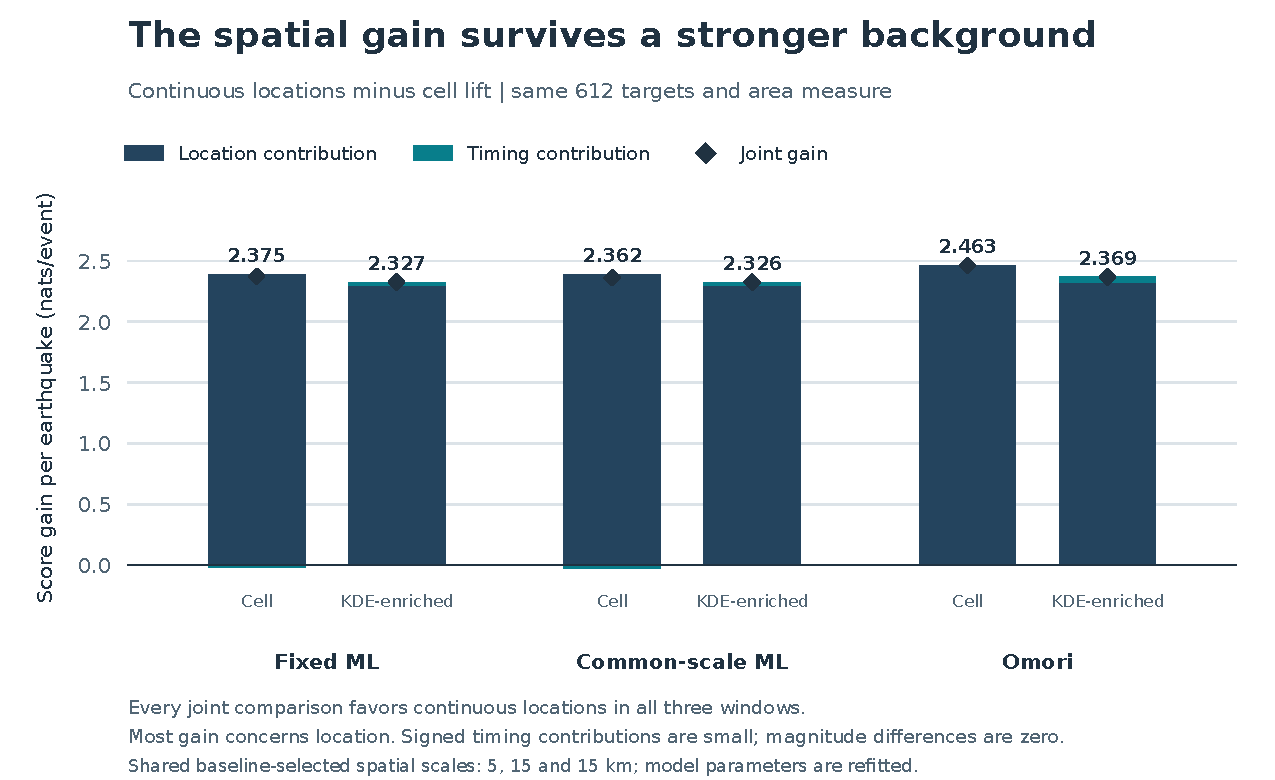
\includegraphics[width=\linewidth,height=.78\textheight,keepaspectratio]{spatial_addendum_iii_fig2_spatial.pdf}
\caption{Continuous-location improvements under both background representations, with location and timing distinguished.}\end{figure}

\section{Combined procedure and scale sensitivity}

Against the current matched fixed-ML/cell-background/lift comparator, Omori with continuous locations gains 1521.255407 joint nats using cell background, or 1554.503812 nats (2.540039 per event) using KDE-enriched background. The latter has +11.530195 timing nats and +1542.973617 net conditional-location nats; magnitude contributes zero. Joint gains are positive in all three windows, but timing changes are -2.961931, +4.108633 and +10.383493. These are direct fitted contrasts, not sums of earlier separate experiments. The previous sealed lift procedure selected its own sigma and is not the present shared-sigma comparator.

Training selected sigma values of 5, 15 and 15 km; KDE bandwidth was 15 km in all three windows. The first sigma lies at the primary grid's lower endpoint. Bounded sensitivity therefore retained separate fixed-ML/continuous fits at 1 and 2 km under both backgrounds. All twelve lost joint score against their primary reference, by 96.988003-308.063524 nats. Some improved timing while losing more location density. These sensitivity fits neither replace the primary models nor constitute an expanded-grid factorial.

\begin{figure}[htbp]\centering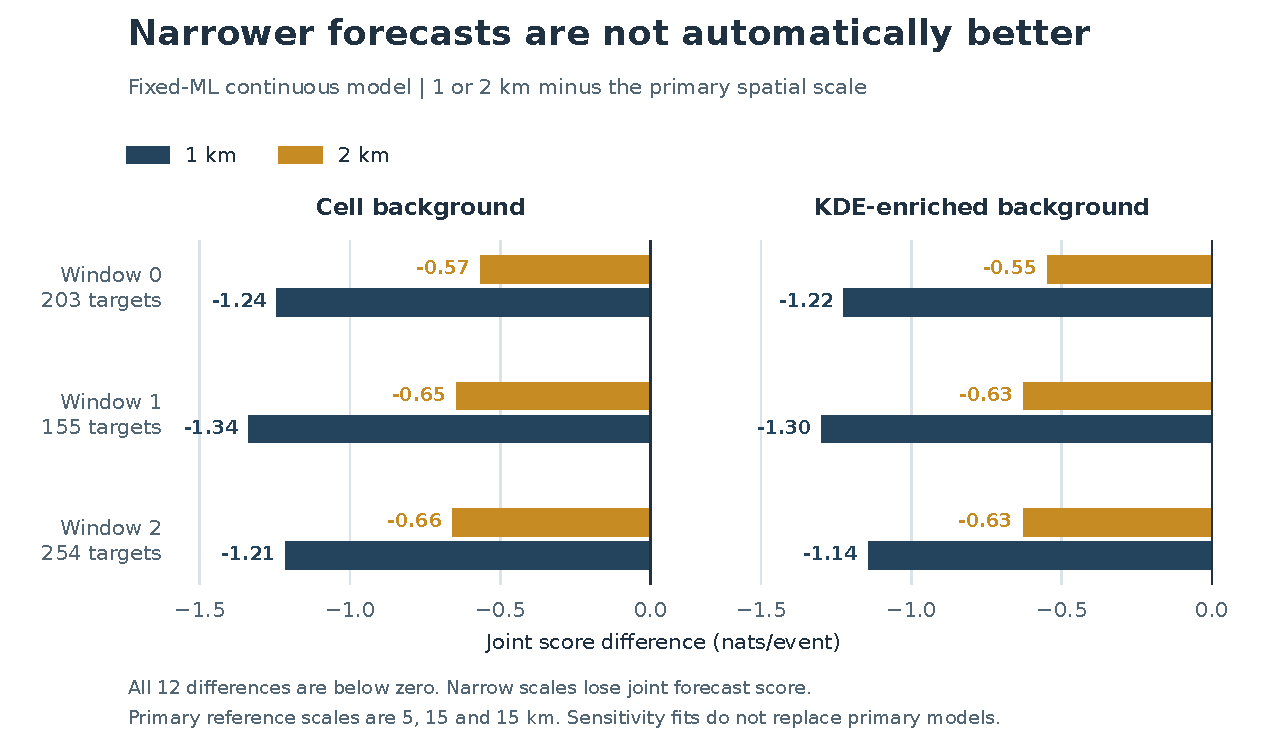
\includegraphics[width=\linewidth,height=.78\textheight,keepaspectratio]{spatial_addendum_iii_fig3_sensitivity.pdf}
\caption{Joint-score losses from the declared 1 and 2 km sensitivity procedures.}\end{figure}

The catalogue has 910 distinct coordinate pairs among 913 events, with three repeated pairs. Serialized decimal places do not establish location accuracy; these results identify neither a physical interaction distance nor a universal optimal bandwidth.

\section{Validation, scope and implications}

All 63 observed procedures and 504 prescribed starts resolved, retaining 579 candidates and 75 exact floors. Including two fixed-seed engineering histories, totals are 87 procedures, 696 starts and solver returns, 803 candidates and 107 floors. Analytic gradients, finite differences, normalization, exact nesting and quadrature checks preceded observed fitting. An independent raw-history auditor reconciled saved scores to within 3.28e-11 nats, below the unchanged 1e-4 tolerance. Near-optimal forecast spread passed the declared gate. Neither multiple starts nor that gate certifies a global optimum.

One initial audit failed because a metadata assertion required exact binary equality between independently solved magnitude-rate estimates differing by six floating-point units. An append-only repair separated exact producer identity from the existing reconstruction tolerance. Independent numerical scores still used raw-derived values; all 326 scientific outputs remained unchanged, with no refits or replacement histories. The audit review and accounting retain that failure and recovery. The reconstructed catalogue rows are now supplied with an executable cohort replay; event-level feature caches are numerical rebuild products. This chapter retains its reviewed spatial aggregates and does not claim a new execution of these spatial fits or their original score audit. Computational-agent review is not external academic peer review.

The strongest supported conclusion is a positive retrospective forecasting ablation: finer offspring-location representation retains a large location-score advantage under a stronger background, while Omori adds a smaller timing improvement against fixed ML in the continuous model. Background and temporal comparisons also contain losses that prevent a blanket preference claim. Constant-Poisson floors are numerical witnesses, not an optimized no-trigger comparator, so this experiment does not establish that physical triggering is present or required. It does not test inhibition.

The same historical windows have been inspected repeatedly; overlapping training prefixes and dependent earthquake histories preclude event-iid confidence intervals or claims of independent replication. Proper held-out scoring does not remove this adaptive-reuse limitation. No Wilks inference, physical causality, immigrant-law recovery or universal scale claim follows. At the time of this factorial study, continuous local inhibition and unused-data replication were design-only follow-ons. The subsequently completed immigrant-only local-inhibition study is reported in Chapter~\ref{ch:local-inhibition}; genuinely unused-data replication remains a separate objective. The current update supplies a bounded positive predictive finding while preserving those outstanding questions and all earlier manuscript conclusions in their original scope.
% Audit-table relocation: app:audit10-factorial
All primary arm-by-window absolute scores are retained in Appendix~\ref{app:audit10-factorial}; its \hyperref[app:audit10-sensitivity]{small-scale sensitivity table} retains every bounded sensitivity fit.

\section{Reproducible geometry and fitting contract}
Let $A_c$ be projected cell area and $N_c,N_z$ the training cell and zone counts. The hierarchical reference obeys
\begin{equation}
 \pi_z=N_z/N,\qquad q(c\mid z)=\frac{N_c+1/2}{N_z+3/2},\qquad
 b_{\rm ref}(z)=\frac{\pi_{z(c)}q(c\mid z(c))}{A_c}\quad(z\in c).
\end{equation}
Writing $D_h(v)=(1+\lVert v\rVert^2/h^2)^{-2}$, define $F_j(h)=\int_D D_h(v-z_j)\,\mathrm dv$. The actual smooth immigrant density and the parent-normalized offspring law are
\begin{align}
 b_{\rm bg}(z)&=0.05b_{\rm ref}(z)+\frac{0.95}{N}\sum_{j=1}^N\frac{D_h(z-z_j)}{F_j(h)},\\
 s_\sigma(z\mid z_j)&=\frac{b_{\rm ref}(z)D_\sigma(z-z_j)}{\int_D b_{\rm ref}(v)D_\sigma(v-z_j)\,\mathrm dv},\\
 W_{cj}&=\frac{\pi_cD_\sigma(v_c-z_j)}{\sum_l\pi_lD_\sigma(v_l-z_j)},\qquad
 s_{\rm lift}(z\mid z_j)=W_{cj}/A_c\quad(z\in c).
\end{align}
Here $v_c$ is the projected rectangle centre and $\pi_c=\pi_{z(c)}q(c\mid z(c))$. Parents retain actual coordinates in both laws; only the lift's target weights use centres. The same KDE-enriched immigrant density is retained even in a lifted offspring arm; its cell-density floor can retain boundary jumps. Leave-one-out selection removes the scored row's identity from both the kernel mixture and hierarchical counts, retains other observations with duplicate coordinates, and normalizes every retained kernel separately. Exact bandwidth ties select the smaller bandwidth. Full-training plug-in nuisance density, including self contributions, is frozen after selection.

The equal-area coordinates are $x=R\cos\phi_0(\lambda-\lambda_0)$ and $y=R(\sin\phi-\sin\phi_0)/\cos\phi_0$, with angular arguments in radians. Euclidean radial isotropy is specific to this projection. Multiplication by piecewise reference geography and finite-domain truncation generally destroys isotropy and translation invariance of the full density. Positive rectangle integrals are checked without clipping invalid values. For any parent, finite-window temporal exposure uses $S(L)-S(U)$ with $L=\max(t_{\rm start}-t_j,0)$ and $U=\max(t_{\rm end}-t_j,0)$; temporal kernels are never renormalized to the evaluation window.

All main fits use the same bounded training-likelihood selection rule. Fixed ML starts span the prescribed amplitude offset, trend and branching schedule. Common-scale ML and Omori initialize shared nuisance coordinates from their same-background/same-geography fixed-ML fit; this is a declared procedure dependency, not held-out selection. The constant-Poisson floor is an admissible numerical witness. Common-scale ML additionally retains the exact fixed-ML floor; Omori and ML are not nested within these finite parameter bounds. Background and continuous/lift families are not declared nested.
% Audit-table relocation: app:audit10-protocol
The complete scalar numerical protocol, prescribed starts, bounds and engineering-control coordinates are retained in Appendix~\ref{app:audit10-protocol}.


\chapter{External Comparisons, Competitive ETAS Benchmarks, Robustness, and Sequence Concentration}
\label{ch:external}
\section{Study overview}

The stronger benchmark defeats the target procedure in both external regions: fitted inverse-power ETAS (EP) exceeds Omori continuous (OC) on joint score in every primary California and Japan test window (while losing one episode in the separate five-episode causal-window backtest in Section~\ref{sec:s06-completed}). OC nevertheless improves California timing against fixed-scale Mittag-Leffler continuous (FC) by 0.119969 nats per target and location against the coarse Omori cell-lift (OL) by 2.140710, over 315 targets. These are different references, and the location gain primarily measures recovery of within-cell density. Japan retains that representation contrast but reverses the OC--FC timing direction in every window, so the registered combined transfer criterion is not demonstrated. California's positive timing contrast is strongly concentrated in one eligible sequence period. Conditional diagnostics also expose OC discrepancies. These inspected and revised archives support retrospective fitted-procedure comparisons, not pristine confirmation or a physical mechanism.

\section{Question, status and relation to the preceding work}

The question is how far the specific forecasting improvements reported in Chapter~\ref{ch:nz-spatial} travel when the region, comparator and diagnostic question change. There are four distinct questions: does a matched ablation retain its direction elsewhere; does the complete procedure beat serious alternatives; do its conditional probabilities resemble the recorded history; and where do the realised score differences occur? A positive answer to one does not answer the others.

Chapter~\ref{ch:nz-spatial} found a large location-score advantage for continuous offspring geography over a cell-lift representation in New Zealand, and a smaller timing advantage for Omori decay over fixed-scale Mittag-Leffler decay within the continuous representation. Its 612 historical targets are context for the programme, not an additional denominator for any table below. The present chapter consolidates subsequent completed studies. Chapter~\ref{ch:local-inhibition} separately reports the local-inhibition extension and its negative observed result. The original manuscript and Addenda I--III remain historical source authorities; the present chapter integrates the completed studies into this unified monograph.

The historical comparisons in this chapter are supported by retained fit, score and audit records. The current public reproduction bundle supplies the recovered catalogue inputs and original fitted states; the reproduction guide identifies each independently executed replay.

\section{Models, forecast object and score}

\subsection{Arm names and what each comparison changes}

The abbreviations are local procedure names, not claims of new model families. All excitation arms share the declared training-only magnitude recipe with productivity exponent r = 0.7 and score the magnitude mark once.

\begingroup\small\setlength{\tabcolsep}{2pt}\renewcommand{\arraystretch}{1.18}
\begin{longtable}{@{}>{\raggedright\arraybackslash}p{0.2280\textwidth}>{\raggedright\arraybackslash}p{0.2280\textwidth}>{\raggedright\arraybackslash}p{0.2280\textwidth}>{\raggedright\arraybackslash}p{0.2280\textwidth}@{}}
\toprule
{}Arm & Temporal law & Offspring geography & Role \\
\midrule\endfirsthead
\toprule
Arm & Temporal law & Offspring geography & Role \\
\midrule\endhead
\midrule\multicolumn{4}{r}{\emph{Continued on next page}}\\
\endfoot
\bottomrule\endlastfoot
{}FC & Fixed-scale Mittag-Leffler & Continuous OC geography & Primary timing reference \\
{}FL & Fixed-scale Mittag-Leffler & Cell-lift & Spatial/context reference \\
{}MC & Free common-scale Mittag-Leffler & Continuous OC geography & Temporal context \\
{}OC & Omori & Continuous OC geography & Frozen target procedure \\
{}OL & Omori & Cell-lift & Primary location reference \\
{}EP & Omori ETAS adaptation & Unweighted inverse-power radial law & Competitive reference \\
{}N0 & No offspring excitation & Smooth background & Refitted no-trigger reference \\
{}LI & Omori plus immigrant attenuation & Continuous OC geography & Inhibition extension in Chapter~\ref{ch:local-inhibition} \\
\end{longtable}\endgroup

The continuous OC offspring density multiplies a radial factor by a fixed training-derived reference density and normalizes over the finite domain separately for each parent. A cell-lift uses target-cell-centre weights and spreads each cell's offspring mass uniformly inside it; actual parent coordinates remain in the calculation. Thus OC-OL is a particular within-domain representation comparison. Both retain smooth immigrant geography. EP instead uses a separately fitted, pure inverse-power offspring kernel, normalized with respect to projected area without OC's reference-density multiplier. OC-EP compares whole procedures with different spatial laws; it is not an isolated temporal-kernel experiment.

The cell-lift and national-routing arms are coarse representation controls. Their losses establish the cost of those discretizations for the declared score, rather than competitive superiority over an equally resolved alternative. The separately fitted EP arm supplies the stronger spatial comparison. Keeping the testing population, forecast object and reference explicit follows the forecast-evaluation distinction emphasized in CSEP methodology \citep{Schorlemmer2007,Zechar2010}.

N0 fixes branching at zero and refits its own background time-rate parameters on training data. It is neither an OC fit with its trigger switched off afterwards nor a constant-Poisson numerical floor. LI attenuates only the immigrant component of OC; its full definition and exact zero-inhibition nesting are given in Chapter~\ref{ch:local-inhibition}.

\subsection{Sequential conditional forecasting}

At each origin, parameters and spatial nuisance choices use training data only and remain fixed during the test window. Every strictly earlier admissible observed event can enter the subsequent history, including earlier events in that test window. This scores a sequential conditional forecast. It does not supply the whole future catalogue at the origin, and it is not an issue-frozen nonhomogeneous Poisson forecast of the complete future path.

The finite domain, parent eligibility, exposure and projected-area measure are shared within each contrast. For an event intensity \(\lambda(t,z)\), its regional ground intensity \(R(t)\), full space-time exposure \(E\), and common magnitude-mark score \(M\), define

\begin{align}
P&=\sum_i\log\lambda(t_i,z_i),&Q&=\sum_i\log R(t_i),\\
E&=\int_{I}\int_D\lambda(t,z)\,\mathrm dz\,\mathrm dt,&C&=-E,\\
S_{\rm time}&=Q+C,&S_{\rm loc}&=P-Q,\\
S_{\rm joint}&=P+C+M=S_{\rm time}+S_{\rm loc}+M.
\end{align}

Higher is better. In a difference between procedures, the signed exposure contribution is minus the difference in E. Quiet periods therefore contribute even when they contain no targets. Common mark differences cancel; a positive location difference is not a statement about magnitude forecasting. Nats are natural-log score units, not percentage accuracy, correlations, causal effects or an estimated percentage of predictable earthquakes. Pooled nats per target divide the sum of window differences by the sum of target counts, never the unweighted average of window means.

This event-logsum and compensator construction is a logarithmic point-process score (the negative of an entropy-loss convention); its differences express log-score gain for the declared observation law \citep{DaleyVereJones2004}.

These symbols are the narrative convention throughout Chapters~\ref{ch:external}--\ref{ch:local-inhibition}. The source-field dictionary maps legacy labels without changing their values: LI's raw pooled key E denotes a point-logsum difference, while sequence timing\_\allowbreak{}compensator denotes a signed difference in nonnegative integrated exposure whose score contribution has the opposite sign. Neither raw name overrides the definitions above.

Primary timing means OC-FC timing; primary location means OC-OL conditional location. These rows use different references and cannot be added to manufacture a combined gain. A direct OC-FL joint contrast, where reported, is a separate comparison.

\section{California: successful matched transfer with uneven contributions}

\subsection{Population and chronological windows}

The repaired California source contains 1,272 canonical unique preferred SCEDC/SCSN records meeting reported M $\geq$ 4.0, latitude 32-37 degrees, longitude -121 to -114 degrees and depth -5 to 40 km. Of these, 106 records in 1981-1985 provide warmup parents. Scored training begins in 1986; expanding training prefixes contain 851, 930 and 1,097 targets. The three half-open UTC test windows contain 79, 167 and 69 targets. Their total is 315 unique held-out targets. Reappearance of this denominator in the benchmark, calibration, concentration and inhibition studies reflects reuse of those same targets, not new samples.

The schema repair retained an earlier stop and changed only acceptance of unused location-quality metadata as opaque printable tokens. All 45 cached official files were reused unchanged; no query, row removal, imputation or forecasting-engine change was needed. The 134 previously rejected occurrences were retained, and none was an M $\geq$ 4 model candidate. Independent reconstruction established equality of the previous model and diagnostic arrays. This establishes lossless handling within the verified snapshot, not universal source completeness or uninspected historical forecasting.

\subsection{Primary results}

\begingroup\footnotesize\setlength{\tabcolsep}{2pt}\renewcommand{\arraystretch}{1.18}
\begin{longtable}{@{}>{\raggedright\arraybackslash}p{0.1800\textwidth}>{\raggedright\arraybackslash}p{0.1800\textwidth}>{\raggedright\arraybackslash}p{0.1800\textwidth}>{\raggedright\arraybackslash}p{0.1800\textwidth}>{\raggedright\arraybackslash}p{0.1800\textwidth}@{}}
\toprule
{}Window (targets) & OC-FC timing nats & Timing nats/target & OC-OL location nats & Location nats/target \\
\midrule\endfirsthead
\toprule
Window (targets) & OC-FC timing nats & Timing nats/target & OC-OL location nats & Location nats/target \\
\midrule\endhead
\midrule\multicolumn{5}{r}{\emph{Continued on next page}}\\
\endfoot
\bottomrule\endlastfoot
{}2011-2016 (79) & +0.099084 & +0.001254 & +91.803255 & +1.162067 \\
{}2016-2021 (167) & +32.722878 & +0.195945 & +465.829993 & +2.789401 \\
{}2021-2026 (69) & +4.968377 & +0.072005 & +116.690274 & +1.691163 \\
{}Pooled (315) & +37.790339 & +0.119969 & +674.323522 & +2.140710 \\
\end{longtable}\endgroup

Both primary directions are positive in all three windows. Timing is nearly tied in the early window; the middle window supplies about 87\% of the total timing difference. The timing pair also has a negative conditional-location difference in the middle window. Positive primary directions therefore do not imply uniformly improved components or a constant effect size.

Of the +674.323522 conditional-location nats, +653.602228 come from within-cell density. This is consistent with the distinction between a continuous density and uniform within-cell offspring mass. It does not establish a similarly large gain in allocation among broad zones or cells, nor general accuracy of individual event locations. Training selected both background bandwidth and inherited offspring scale at 5 km, the lower grid endpoint in every California fold. This is a boundary of the declared grid, not an identified physical interaction distance or proof of coordinate accuracy.

Thus about 96.93\% of this location contrast comes from within-cell density. The analogous higher-threshold share is about 95.48\%. These large shares are consequences of the particular uniform-within-cell reference; they are not percentages of correctly predicted locations or evidence of a physical interaction distance.

For context, OC-MC gains +21.177884 joint nats (+0.067231 per target), FC-FL gains +671.244340 location nats (+2.130934), and the direct OC-FL comparison gains +747.800021 joint nats (+2.373968). Each wins all three windows. Their reference arms and score components differ; these results are not additive.

\begin{figure}[tbp]\centering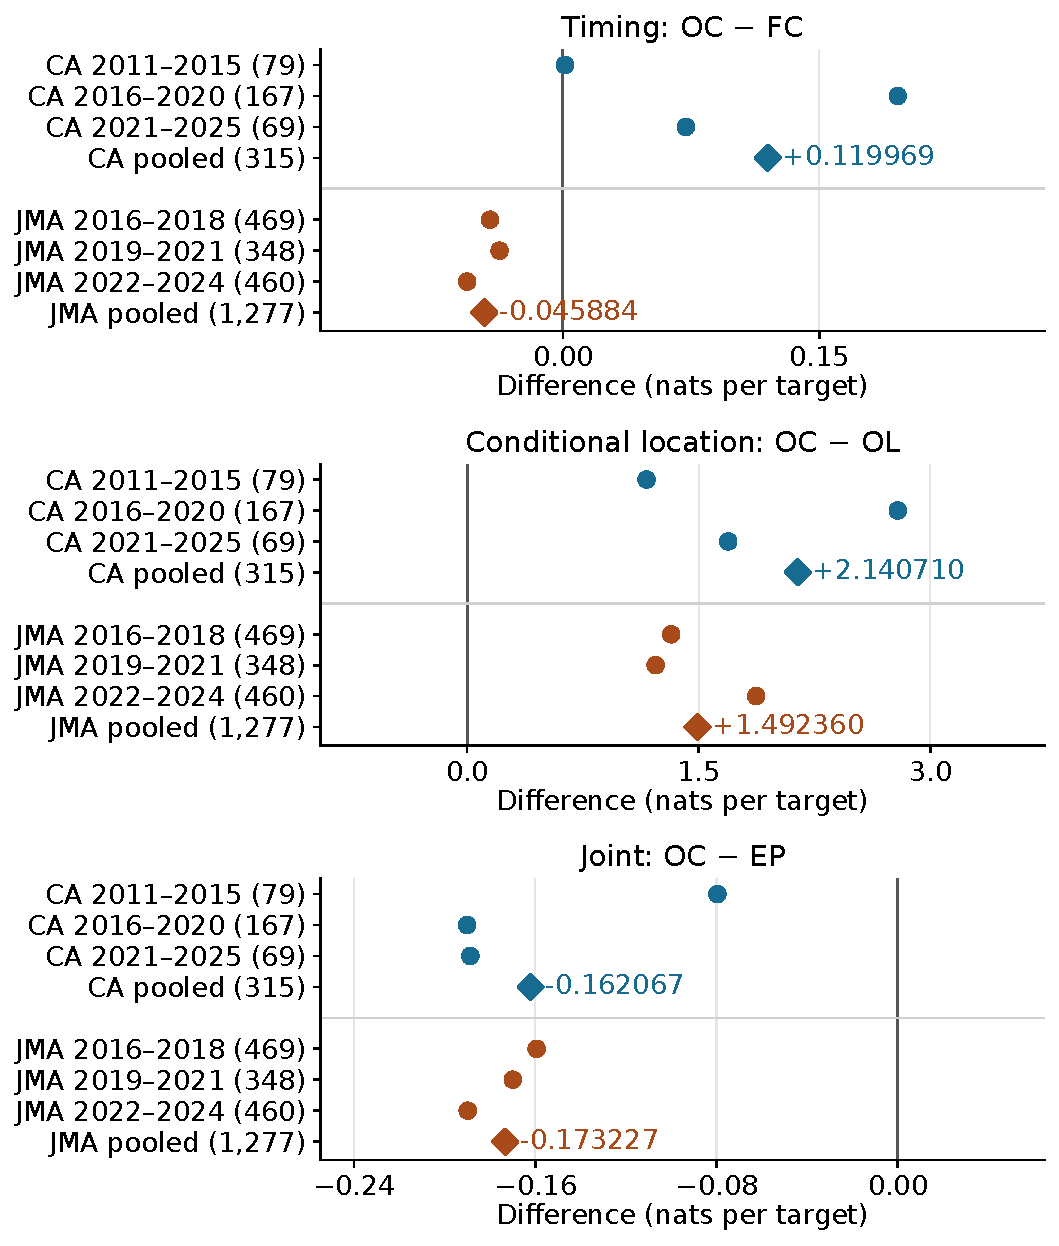
\includegraphics[width=\linewidth,height=.78\textheight,keepaspectratio]{spatial_addendum_iv_matched_regional_contrasts.pdf}
\caption{Matched timing and location comparisons in California and Japan. Realised proper-score contrasts from the original California M $\geq$ 4 cohort (315 targets) and the JMA reported-primary M $\geq$ 4.5 complete-case cohort (1,277 records). Each panel has its own reference and horizontal scale. Timing compares OC with FC; conditional location compares OC with OL; joint compares OC with EP. Pooled diamonds divide summed window nats by the regional total. California uses UTC years and JMA source-JST years. Different-reference columns and geographies are not added. Related retrospective windows have no event-iid uncertainty intervals.}\end{figure}



The California accepted report supplies source selection, repair chronology and complete comparison components.

\section{Stronger benchmarks change the conclusion}

OC exceeds the refitted N0 procedure by +1694.942967 joint nats over 315 targets, but EP exceeds OC in each primary California test window. The same 315 targets, common mark law and frozen OC states are used. EP was independently fitted using training data; it was not selected as a replacement downstream forecast after inspecting these scores.

\begingroup\footnotesize\setlength{\tabcolsep}{2pt}\renewcommand{\arraystretch}{1.18}
\begin{longtable}{@{}>{\raggedright\arraybackslash}p{0.1800\textwidth}>{\raggedright\arraybackslash}p{0.1800\textwidth}>{\raggedright\arraybackslash}p{0.1800\textwidth}>{\raggedright\arraybackslash}p{0.1800\textwidth}>{\raggedright\arraybackslash}p{0.1800\textwidth}@{}}
\toprule
{}OC minus reference, pooled 315 & Joint nats & Timing nats & Location nats & Joint nats/target \\
\midrule\endfirsthead
\toprule
OC minus reference, pooled 315 & Joint nats & Timing nats & Location nats & Joint nats/target \\
\midrule\endhead
\midrule\multicolumn{5}{r}{\emph{Continued on next page}}\\
\endfoot
\bottomrule\endlastfoot
{}N0 & +1694.94 & +894.846 & +800.097 & +5.38077 \\
{}EP & -51.0512 & +0.33625 & -51.3875 & -0.162067 \\
\end{longtable}\endgroup

OC-N0 joint, timing and location differences are positive in all three windows. This supplies a serious no-trigger predictive comparison that a numerical Poisson floor could not supply. Its middle window contributes about 77.49\% of the joint gain. The comparison is between complete procedures with shared trained geography; it does not establish causal triggering or identify immigrant labels.

OC-EP joint differences are -6.288819, -31.742512 and -13.019873 nats. Conditional location loses in each window. The pooled timing difference is only +0.001067 nats per target, with a small middle-window loss; EP's joint advantage is mainly spatial. Therefore the finding that OC improves on OL cannot be promoted into superiority over the strongest evaluated spatial benchmark.

The decomposition also matters. Against EP, the point-event difference is -54.591677 nats, partly offset by a +3.540472 signed exposure contribution. Against N0, these are +1612.690857 and +82.252111. A point-only comparison would omit quiet-period exposure. The common magnitude law contributes equally to every arm, so these joint-score contrasts measure space--time occurrence forecasting; all mark differences are zero.

\begin{figure}[tbp]\centering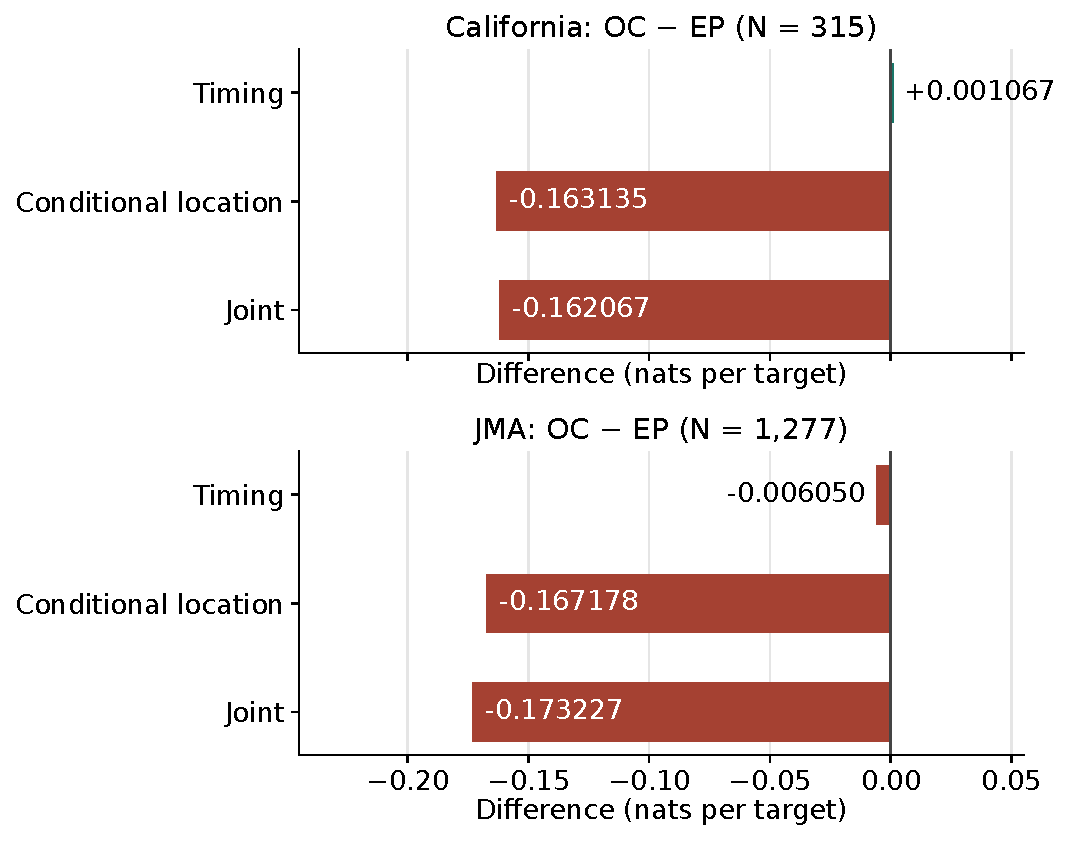
\includegraphics[width=\linewidth,height=.78\textheight,keepaspectratio]{spatial_addendum_iv_ep_score_components.pdf}
\caption{Timing and location components of OC relative to EP in California and Japan. Pooled OC-minus-EP timing, conditional-location and joint differences, normalized separately by 315 California targets and 1,277 JMA records. Joint equals timing plus conditional location because mark differences are zero. California has a tiny timing edge; JMA has a timing loss. The larger location deficit accounts for most joint loss in both regions. EP is a separately fitted complete procedure; relative superiority establishes neither EP calibration nor an isolated temporal-kernel effect.}\end{figure}



The competitive benchmark report is the numeric authority for this section. The LI replay in Chapter~\ref{ch:local-inhibition} is separately sourced and differs at floating-point scale; it does not replace these archived benchmark values.

\section{Conditional adequacy is a separate question}
The frozen OC conditional simulation and its complete coordinate results are developed in Chapter~\ref{ch:calibration}. Relative scores here do not supply an adequacy result for either OC or EP.
\section{Robustness and concentration answer narrower questions}

\subsection{A higher threshold retains directions under a changed observation law}

The base annual accounting retains every event's original history and all exposure, including years with zero targets. It refits no base parameter. A separately admitted M $\geq$ 4.5 sensitivity rebuilds the population, eligible histories, training estimates, mark law and fitted procedures. Its 391-record population includes 33 warmup parents; training counts are 271, 287 and 340, and test counts 16, 53 and 18, totaling 87. Those 87 are a higher-threshold subset of the California history, not 87 additional independent records to add to 315.

The sensitivity applies the threshold to the provider's exact preferred-magnitude token before converting magnitude excess to binary64. Its relative mark-bin cutoff remains 0.5, corresponding to M5.0. Domain, depth/type/time rules, strict earlier-parent eligibility and $r=0.7$ are retained. Beta, hierarchical reference masses, KDE bandwidth and model parameters are re-estimated from each training prefix. Six fixed-ML continuous spatial selectors, a lifted prerequisite, common-scale ML and the two Omori procedures remain in the roster; the selected fixed-ML arm is an alias of its winning selector, not an extra fit. The first fold served as the resource/correctness pilot, and its accepted files were reused without score-based continuation or replacement. The 87 targets fall below the inherited descriptive reference of 100 in total; 16 and 18 also fall below 20 per window. Those pragmatic references are not power guarantees.

\begingroup\footnotesize\setlength{\tabcolsep}{2pt}\renewcommand{\arraystretch}{1.18}
\begin{longtable}{@{}>{\raggedright\arraybackslash}p{0.1800\textwidth}>{\raggedright\arraybackslash}p{0.1800\textwidth}>{\raggedright\arraybackslash}p{0.1800\textwidth}>{\raggedright\arraybackslash}p{0.1800\textwidth}>{\raggedright\arraybackslash}p{0.1800\textwidth}@{}}
\toprule
{}Primary comparison and component & M $\geq$ 4.0 nats/target (315) & M $\geq$ 4.5 nats/target (87) & M $\geq$ 4.5 total nats & Positive windows \\
\midrule\endfirsthead
\toprule
Primary comparison and component & M $\geq$ 4.0 nats/target (315) & M $\geq$ 4.5 nats/target (87) & M $\geq$ 4.5 total nats & Positive windows \\
\midrule\endhead
\midrule\multicolumn{5}{r}{\emph{Continued on next page}}\\
\endfoot
\bottomrule\endlastfoot
{}OC-FC timing & +0.119969 & +0.152292 & +13.2494 & 3/3 \\
{}OC-OL location & +2.14071 & +2.12387 & +184.776 & 3/3 \\
{}OC-MC joint context & +0.0672314 & +0.0775184 & +6.7441 & 2/3 \\
\end{longtable}\endgroup

The first higher-threshold OC-MC joint difference is -0.626348 nats, and its OC-FC timing gain is only +0.077968 total nats. The two smaller test windows contain fewer than 20 targets. The threshold columns describe distinct complete procedures and target/parent laws; their difference is not a paired performance improvement or a threshold selection result. EP was not refitted or evaluated in this sensitivity, and no new calibration was performed.

Against OL, the higher-threshold location decomposition is +5.881781 zone, +2.472120 conditional-cell and +176.422568 within-cell nats. Its OC--FC timing decomposition is +14.762895 event-ground nats minus 1.513472 integrated-exposure nats; OC--MC joint gain comprises +5.992897 timing and +0.751200 location nats. Each decomposition retains its own reference.

Preferred magnitudes mix magnitude types and are not homogeneous moment magnitude. Count eligibility does not establish physical detection completeness. The source provides no defensible numerical location covariance or empirical location-error distribution; no perturbation law was invented from quality codes or decimal places. No independent alternate historical snapshot was admitted. The sensitivity therefore supports direction under one specified observation-law change, not general robustness to catalogue uncertainty.

\begin{figure}[tbp]\centering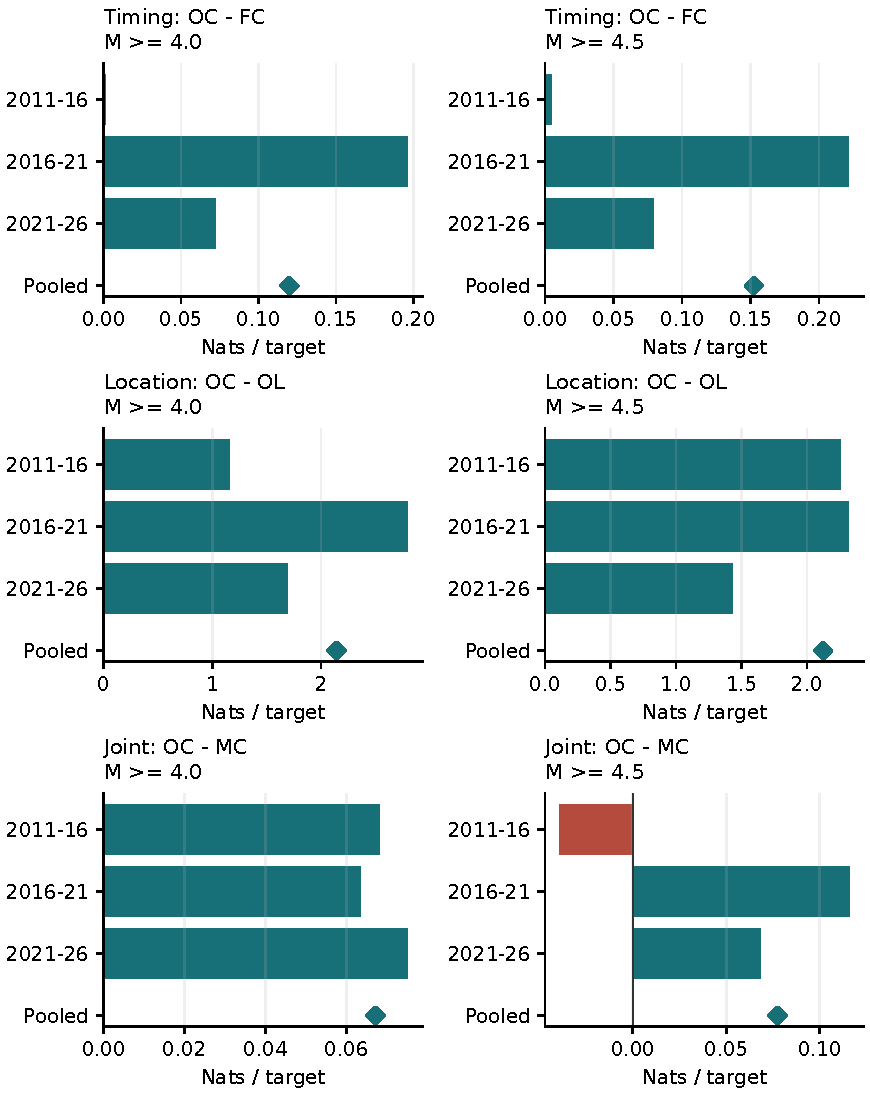
\includegraphics[width=\linewidth,height=.78\textheight,keepaspectratio]{spatial_detail_window_primary_nats_per_target_m4_m45_v1.pdf}
\caption{Fixed-window and event-weighted pooled primary score contrasts per target under M $\geq$ 4.0 and M $\geq$ 4.5. Bars retain the three windows and pooled diamonds divide summed nats by 315 or 87 targets. Each component uses its named reference; the negative early OC--MC joint contrast is retained. Cross-threshold differences are descriptive, not paired performance gains.}\end{figure}


\subsection{Annual gains are concentrated}

In the base analysis, calendar 2019 has 116 targets and contributes +29.280597 OC-FC timing nats, +392.773429 OC-OL location nats and +7.979400 OC-MC joint nats. At M $\geq$ 4.5, 37 targets in that year contribute +10.977080, +112.007721 and +5.288450 respectively. These are separate contrast/component columns. Negative annual contributions remain in the accepted tables.

The base 2019 signed shares are 77.48\%, 58.247\% and 37.678\% of their respective pooled contrasts, including negative years in each denominator. At the higher threshold, ten of fifteen annual timing contributions are negative. Zero-target years 2015 and 2017 retain their exposure terms; their per-target means are undefined, not zero. Appendix~\ref{app:audit11-annual} retains every annual row and both thresholds.

Annual partitions preserve subsequent parent history. They do not estimate a counterfactual catalogue without a sequence. Their purpose is to locate realised score contributions, not to remove inconvenient years or create independent replications. The robustness decision report records the full design and absent sensitivity laws.

\begin{figure}[tbp]\centering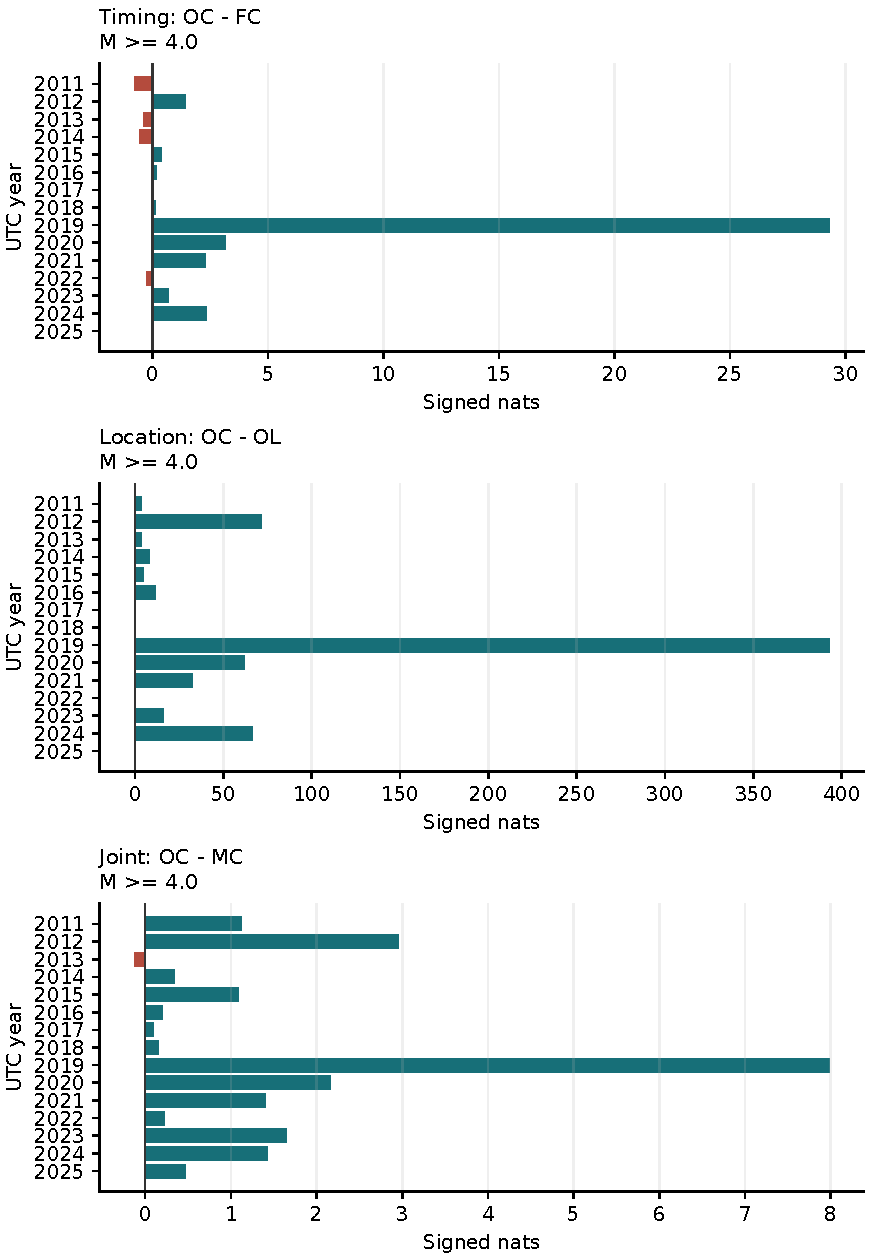
\includegraphics[width=\linewidth,height=.78\textheight,keepaspectratio]{spatial_detail_annual_primary_contributions_v1.pdf}
\caption{Annual signed score contributions for all fifteen California M $\geq$ 4.0 test years under the three distinct named comparisons. The panels use their own references; negative years remain. These are contributions to realised scores, not independent annual replications.}\end{figure}

\begin{figure}[tbp]\centering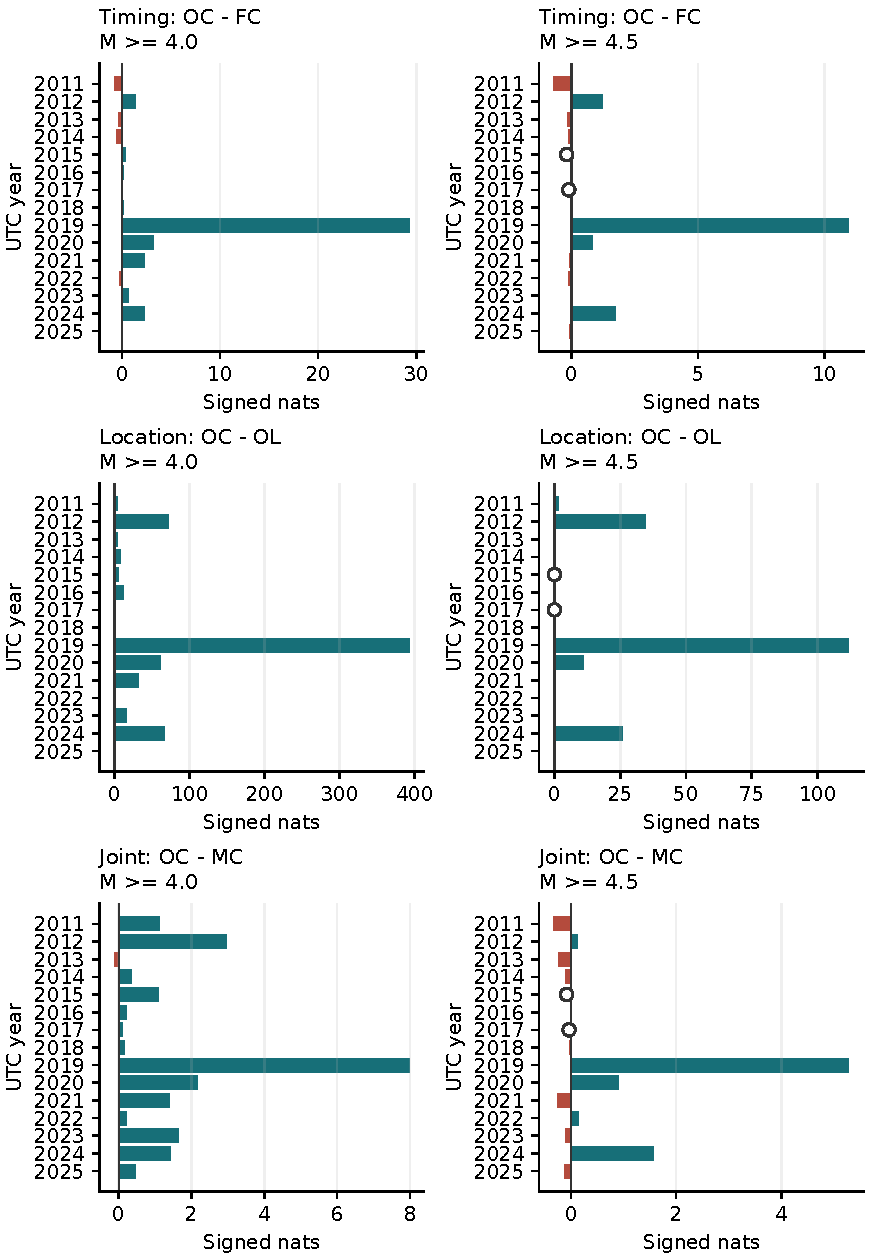
\includegraphics[width=\linewidth,height=.78\textheight,keepaspectratio]{spatial_detail_annual_primary_contributions_m4_m45_v1.pdf}
\caption{Annual signed score contributions under M $\geq$ 4.0 and M $\geq$ 4.5. All fifteen years remain; hollow circles identify zero-target years whose exposure contributions are retained. Component panels have distinct references. The nested populations and refitted procedures do not define a paired threshold gain.}\end{figure}


\subsection{One eligible active episode, with the complete complement retained}
\label{sec:calendar-sequence-partition}

The finer sequence partition was chosen after annual inspection, including 2019. The frozen metadata rule marks regional time active when an admissible M $\geq$ 6 anchor at u satisfies u < t $\leq$ u + 30 days. Overlapping anchor windows merge globally before fold clipping; eligible prehistory is retained. This is a regional time partition, not a causal or spatial aftershock classification. The initial anchor belongs to the complement unless an earlier anchor already activates it.

Only one eligible episode intersects the scored test windows: a Ridgecrest-associated union lasting 31.406991204 days with 110 targets. The other 205 targets and 5,447.593008796 exposure days remain the complete complement. Thirteen anchors and ten global episodes occur in the admitted chronology, but nine episodes lie in pre-test history. They are not nine additional scored replications.

The active period contributes +30.058155064 of the +37.790339259 pooled OC--FC timing nats, approximately 79.54\%. With only one scored episode, the archive cannot estimate reproducibility of that concentration across sequences. Integer UTC membership and global interval merging are fixed before fold clipping. One of the two test anchor targets is active and the other is in the complement; event-only anchor scores are not part of the public aggregate.

\begingroup\footnotesize\setlength{\tabcolsep}{2pt}\renewcommand{\arraystretch}{1.18}
\begin{longtable}{@{}>{\raggedright\arraybackslash}p{0.1800\textwidth}>{\raggedright\arraybackslash}p{0.1800\textwidth}>{\raggedright\arraybackslash}p{0.1800\textwidth}>{\raggedright\arraybackslash}p{0.1800\textwidth}>{\raggedright\arraybackslash}p{0.1800\textwidth}@{}}
\toprule
{}Pooled category & Targets & OC-FC timing nats & OC-OL location nats & OC-MC joint nats \\
\midrule\endfirsthead
\toprule
Pooled category & Targets & OC-FC timing nats & OC-OL location nats & OC-MC joint nats \\
\midrule\endhead
\midrule\multicolumn{5}{r}{\emph{Continued on next page}}\\
\endfoot
\bottomrule\endlastfoot
{}Active period & 110 & +30.0582 & +375.945 & +9.87815 \\
{}Complete complement & 205 & +7.73218 & +298.379 & +11.2997 \\
{}Full original pool & 315 & +37.7903 & +674.324 & +21.1779 \\
\end{longtable}\endgroup

The six-target calendar-2019 complement is the non-active portion of the 116-target UTC calendar year 2019 within primary Fold 1, distinct from the 127-target causal-origin block and its 16-target complement in Section~\ref{sec:s06-completed}. This calendar-year complement has -0.777558 timing nats and -1.898745 OC-MC joint nats, although its location contribution is positive. The annual timing and MC-context gains therefore arise in the active period. Across the full fifteen test years, all three contextual totals remain positive in the complement; concentration does not mean every contextual gain is confined to that episode.

The stronger reference still wins both partitions. OC-EP joint score is -18.372230 nats in the active period and -32.678975 in the complete complement. Its active timing difference is -0.806683 and location difference -17.565547. Complement timing is +1.142932, outweighed by -33.821907 location nats. All original parents and full-domain exposure remain in every score; event-only scoring would answer a different question. The sequence audit report retains empty active rows, exact exposure accounting and the full partition.

The complete partition tables in Appendix~\ref{app:audit11-sequence} retain empty active periods, full-domain exposures and absolute arm scores. Calendar-2019 and pooled rows repeat portions of the original folds for reporting and must not be added to them. The sequence partition changes neither the original fifteen selected states nor their eligible parent histories.

\section{Japan: spatial direction transfers, combined criterion does not}

\subsection{The reported-record target}

The JMA analysis processes 19 local annual archives for source-JST years 2006-2024. Its 4,019,138 source records yield 4,602 usable study records. The target requires agency J, natural subsidiary 1, determination K/k/A, allowed primary magnitude types J/D/V/d/v, observed numeric primary reported M $\geq$ 4.5, depth 0-60 km and the fixed projected region. Primary and secondary magnitudes remain separate. This is an observed primary complete-case reported-record cohort, not homogeneous Mw, inferred latent magnitudes or proof of physical completeness.

Inspection identified 41,278 initially unresolved target observations: 41,277 with missing/undetermined primary information alone and one with an additional depth issue. An explicit, inspection-informed restriction requires numeric observed primary magnitude and an allowed primary type. It was documented and independently reviewed before fitting. Those records receive no assigned latent magnitude and are not asserted to be physically small. No complete target row was added, removed or modified by that clarification. One auxiliary depth-ambiguous subthreshold record remains unusable for diagnostics and has zero target, parent or beta-observation effect.

The 496 records in 2006-2010 supply warmup only. The following training prefixes and disjoint test windows use exact source-JST boundaries.

\begingroup\footnotesize\setlength{\tabcolsep}{2pt}\renewcommand{\arraystretch}{1.18}
\begin{longtable}{@{}>{\raggedright\arraybackslash}p{0.1800\textwidth}>{\raggedright\arraybackslash}p{0.1800\textwidth}>{\raggedright\arraybackslash}p{0.1800\textwidth}>{\raggedright\arraybackslash}p{0.1800\textwidth}>{\raggedright\arraybackslash}p{0.1800\textwidth}@{}}
\toprule
{}Origin & Scored training years & Training records & Test years & Test records \\
\midrule\endfirsthead
\toprule
Origin & Scored training years & Training records & Test years & Test records \\
\midrule\endhead
\midrule\multicolumn{5}{r}{\emph{Continued on next page}}\\
\endfoot
\bottomrule\endlastfoot
{}2016 & 2011-2015 & 2,829 & 2016-2018 & 469 \\
{}2019 & 2011-2018 & 3,298 & 2019-2021 & 348 \\
{}2022 & 2011-2021 & 3,646 & 2022-2024 & 460 \\
\end{longtable}\endgroup

The total scored denominator is 1,277. These are revised local records; catalogue inspection and observation adjudication preclude a pristine as-issued holdout claim. The JMA processing report gives the source restrictions and exact accounting.

\subsection{Descriptive transfer rule and competitive context}

The combined descriptive transfer rule requires both primary contrasts to exceed +0.0006 pooled total nats and each to be positive in at least two of three folds after audit pass. That threshold allows the declared numerical score tolerance; it is not a statistical significance boundary. The EP joint comparison is separate competitive context.

The $0.0006$ threshold allows $0.0001$ nat for each of two arm scores across three folds. It is a numerical comparison rule, not evidence that the three windows or their events are independent tests.

\begingroup\footnotesize\setlength{\tabcolsep}{2pt}\renewcommand{\arraystretch}{1.18}
\begin{longtable}{@{}>{\raggedright\arraybackslash}p{0.1800\textwidth}>{\raggedright\arraybackslash}p{0.1800\textwidth}>{\raggedright\arraybackslash}p{0.1800\textwidth}>{\raggedright\arraybackslash}p{0.1800\textwidth}>{\raggedright\arraybackslash}p{0.1800\textwidth}@{}}
\toprule
{}Comparison and component & Total nats & Nats/record (1,277) & Direction in windows & Interpretation \\
\midrule\endfirsthead
\toprule
Comparison and component & Total nats & Nats/record (1,277) & Direction in windows & Interpretation \\
\midrule\endhead
\midrule\multicolumn{5}{r}{\emph{Continued on next page}}\\
\endfoot
\bottomrule\endlastfoot
{}OC-FC timing & -58.5935 & -0.0458837 & Negative 3/3 & Timing direction reverses \\
{}OC-OL location & +1905.74 & +1.49236 & Positive 3/3 & Spatial direction transfers \\
{}OC-EP joint & -221.211 & -0.173227 & Negative 3/3 & Strong reference still wins \\
{}OC-MC joint context & -49.1946 & -0.0385236 & Negative 3/3 & No universal Omori preference \\
{}FC-FL location context & +1847.64 & +1.44686 & Positive 3/3 & Spatial result also under FC \\
\end{longtable}\endgroup

The registered combined criterion is \textbf{not demonstrated}. OC-FC timing losses are approximately -19.9765, -12.8718 and -25.7452 nats. OC-OL location gains are approximately +619.711, +424.797 and +861.235. A large location total cannot compensate for a timing requirement with the wrong sign, and primary contrasts with different references must not be added.

EP exceeds OC jointly in all three windows. Conditional location accounts for 213.485907 of the 221.211492-nat deficit. OC also exceeds N0 on pooled joint score, but the strong-reference failure remains. These findings support a useful continuous-versus-lifted representation contrast while qualifying temporal transfer and overall competitive performance.

All background bandwidth selectors choose the lower 5 km endpoint, while FC spatial-scale selectors choose the interior 15 km value. The background trend slope reaches its lower bound for 7, 6 and 2 of seven models in the three folds. Results apply to the frozen grids and bounds; these choices do not identify physical length scales or measurement precision. The JMA forecast report retains full components, annual accounting and the registered decision.

Appendix~\ref{app:audit11-jma} retains all seven pooled contrasts and their three window differences, including OC--FL and OC--N0. The nine annual source-JST blocks retain the same counts and all canonical score/exposure components. No Powell recovery was needed for the 288 accepted L-BFGS-B returns. The filesystem retry reused seven completed procedures byte-for-byte and restored one written floor without reevaluation; it did not change the scientific objective or selection rule.

\section{Consolidated implications and limits}

The completed evidence separates five conclusions. First, continuous offspring geography repeatedly improves conditional location relative to the declared cell-lift procedure, including California's higher-threshold sensitivity and the JMA reported-record cohort. Second, Omori's timing advantage over fixed-scale ML is conditional: positive in the original New Zealand/California comparisons, but negative in every JMA window. Third, excitation improves relative scores over a serious refitted no-trigger baseline, while EP beats OC on joint score in the primary California and Japan folds, mainly through location. Fourth, OC's conditional diagnostics disclose material discrepancies, so relative gains are not adequate-probability certification. Fifth, California gains are uneven and concentrated, with only one eligible scored sequence period and substantial full-complement contributions.

The historical archives have been inspected, processed and revised; later studies adaptively reuse outcomes and related chronological windows. Frozen training/test calculations within a study do not erase that programme-level reuse. Overlapping training prefixes, earthquake dependence and small numbers of windows preclude event-iid confidence intervals and broad independent-replication claims. No Wilks inference, causal triggering claim, recovered immigrant law, physical stress range or absolute calibration result follows. Magnitude-type mixtures, reported-coordinate observation laws, finite-domain parent omissions, plug-in background estimates and grid/boundary choices remain material.


\section{Numerical custody and review scope}

Numerical agreement supports the reported calculations; it does not independently replicate earthquake science. The California source repair accounted for 30 procedures and 240 starts. The separate benchmark audited all six new fit procedures and reconciled scores within 8.19e-11 nats. The higher-threshold sensitivity accounted for 30 procedures and 240 starts, reconciling within 1.13e-11 nats. The sequence audit retained all 315 targets and passed 7,128 component checks with maximum discrepancy 4.55e-13 nats. These are different validation rosters and are not independent research samples to add together.

JMA fitting resolved 36 procedures, 288 starts, 42 floors and 330 slots. Maximum independently reconstructed score disagreement was 1.82e-10 nats against a 1e-4-nat tolerance; maximum stored near-optimal spread was 3.75e-5 nats per record against a strict 0.01 gate. A retained atomic-save interruption was repaired by bounded filesystem retry, preserving completed states without refitting. Other historical failures and recoveries remain in the source reports. Multistart completion and near-optimal-set stability are not global optimization certificates or uncertainty intervals.

The public reproduction bundle now reconstructs the California and Japan cohorts from the original provider records, including source-row identities, exclusion accounting, exact clocks and chronological partitions. The Japanese bundle also supplies recovered fitted states and the explicit projected-region predicate. The current evidence index retains the source pins, unchanged display scalars, source-specific field dictionary and claim bindings. The readable scientific protocol subset supplies the LI law, clocks and fitting contract used in Chapter~\ref{ch:local-inhibition}. The review guide separates these executed cohort replays from regional model refitting and scoring; rebuilding a cohort does not itself rerun its benchmark fits. Rebuildable event caches are outputs of the numerical pipeline, rather than required private inputs.

The detailed numerical record is organized once in Appendix~\ref{app:audit11}. It contains the annual, higher-threshold, sequence-partition and JMA backup tables, with their source-specific denominators and exposure signs; the standalone decision-report narratives are not repeated here.


\section{Completed four-arm spatial comparison}

\label{sec:s03-completed}

\textit{Numerical status: all folds passed their saved custody and score-decomposition checks, and the predeclared independent California-fold sample passed. Acceptance uses sampled validation, not independent raw replay of every fit.}

The comparison contains three California folds with 315 targets and three New Zealand folds with 612 targets. Four procedures are evaluated in each fold: arm 1 uses the reference-density-weighted rational offspring kernel and inherited KDE background; arm 2 removes reference-density weighting; arm 3 adds identity-based leave-one-out background fitting; arm 4 uses the unweighted EP offspring shape with the inherited background procedure. The temporal and mark parameters remain training-selected and fixed. Background level, trend and reproduction coefficient are refitted under the declared arm-specific normalization. California uses the archived training-selected EP spatial scale and shape. The New Zealand OC archives did not contain EP spatial parameters, so a separate training-only prerequisite estimated these missing nuisance parameters before the four-arm comparison. Those values were then frozen: each final arm optimizes only background level, trend and reproduction coefficient. This prerequisite is an explicit addition to the original execution specification, not a claim that the entire preparation fitted only three parameters.

\begin{table}[htbp]\centering

\caption{Held-out joint log-score contrasts in nats. Positive values favour the first named arm. Arm labels follow the text.}\label{tab:s03-completed}

\begin{tabular}{llrrrrr}\toprule Region & Fold & Targets & $2-1$ & $3-2$ & $4-2$ & $4-1$\\\midrule

CA & 0 & 79 & -0.2962 & 1.4515 & 6.3629 & 6.0668 \\

CA & 1 & 167 & 1.0722 & 3.1070 & 29.9884 & 31.0606 \\

CA & 2 & 69 & 0.2776 & 0.7288 & 12.6035 & 12.8811 \\

NZ & 0 & 203 & 0.3421 & 2.1881 & 17.9074 & 18.2495 \\

NZ & 1 & 155 & 33.2980 & -0.3822 & -0.0583 & 33.2397 \\

NZ & 2 & 254 & -1.2518 & -3.2235 & 0.0346 & -1.2172 \\

\bottomrule\end{tabular}\end{table}

\begin{table}[htbp]\centering

\caption{Regional totals for EP minus the OC baseline, in nats. The common mark score cancels.}

\begin{tabular}{lrrr}\toprule Region & Timing & Location & Joint\\\midrule

CA & -0.8205 & 50.8289 & 50.0085 \\

NZ & 2.1452 & 48.1269 & 50.2721 \\

\bottomrule\end{tabular}\end{table}

The contrasts are descriptive comparisons of fitted procedures, not additive causal contributions. In particular, arm 4 minus arm 3 changes the offspring model and the background fitting procedure; it is not a pure tail effect. Arm 4 minus arm 2 is the direct EP versus unweighted-rational comparison with the same background procedure. The identity $(4-1)=(2-1)+(3-2)+(4-3)$ is exact bookkeeping, whereas $(2-1)+(3-2)+(4-2)$ is not the total. Refitting the shared nuisance coefficients further prevents a mechanical causal attribution to a single feature.

All finite retained-state and near-optimal forecast checks are supplied in \path{reproduction/regional/original_completion_20261101.zip}, with planned denominators retained. The closure verification checks the exact frozen spatial parameters, common temporal and mark parameters, three-coordinate final fits, and training-only winner selection across all six folds. It verifies original and portable case byte identities separately and requires exact parsed-content equality; serialization differences are not treated as changed scientific inputs. This is retrospective verification of the saved contract, not a new fit or a fresh validation cohort. The acceptance plan combines a predeclared independent raw geometry/score sample for California fold zero with saved custody, start coverage, selection and score-decomposition checks across all folds. It does not claim independent raw replay of every fit or New Zealand shape prerequisite. New Zealand results retain the archive-reuse disclosure; they are not a fresh untouched holdout.

\begin{figure}[htbp]\centering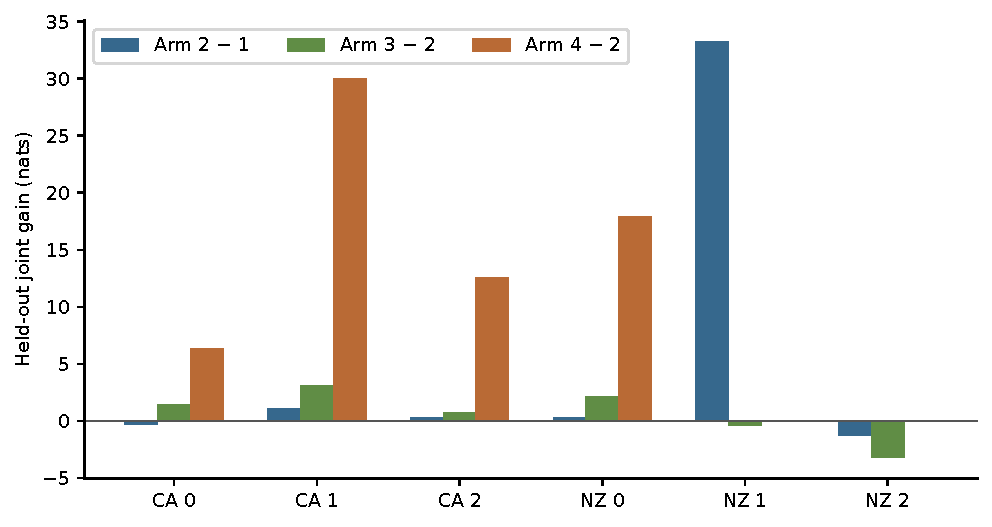
\includegraphics[width=\textwidth]{s03_completed_joint_contrasts.pdf}\caption{Saved held-out joint contrasts across all six folds. Each fold has its own refitted nuisance coefficients; these differences are not a causal mechanism decomposition. Saved custody checks and independent sampled raw validation passed.}\end{figure}


\section{Causal-window California backtests and JMA trend ablation}

\label{sec:s06-completed}

The California and JMA values in this section are recovered original fit and score outputs with checked hashes and source identities. The fitting and rescoring described below belong to the original study; this edition does not recompute them. The original audit coverage is retained.

The completed California map contains five eligible episodes, in 1994, 1999, 2004, 2010 and 2019. The two 1992 episodes are excluded by the predeclared training-count or zone-adequacy rule, not silently replaced by a more favourable sequence. Training expands from 1986 up to, but not including, each episode origin; the parent history retains the 1981 warmup. Each scored block ends at the earlier of the next eligible origin, one year after its origin, or the coverage cutoff. Parameters, spatial scale and nuisance inputs are selected only on the preceding training prefix.

The $M\geq6$ episode origins were identified retrospectively from the catalogue. The roster is retrospective and exploratory. Overlapping training histories and a common archive mean that the five episodes are not independent replications. The active partition is the union of declared episode time intervals, and its complement fills the rest of the scored block; it does not causally label individual earthquakes as aftershocks.

\begin{table}[htbp]\centering\caption{Held-out joint scores (nats) on the five eligible California blocks. Higher is better. These descriptive scores have no confidence intervals.}\label{tab:s06-ca}

\begin{tabular}{lrrrrr}\toprule Year & Targets & FC & MC & OC & EP\\\midrule

1994 & 64 & -527.0462 & -525.5013 & -526.7452 & -521.5603 \\

1999 & 75 & -551.4448 & -545.6841 & -540.1365 & -521.8412 \\

2004 & 30 & -349.2570 & -347.5086 & -347.8333 & -341.1560 \\

2010 & 125 & -1044.6385 & -1055.3761 & -1050.2614 & -1059.1042 \\

2019 & 127 & -696.3825 & -679.3514 & -670.2133 & -647.9267 \\

\bottomrule\end{tabular}\end{table}

\begin{table}[htbp]\centering\caption{OC minus FC joint contrasts, partitioned without changing fitted parameters. Full equals active plus complement, subject to the saved numerical tolerance. These contrasts are descriptive; no confidence intervals are supplied.}

\begin{tabular}{lrrrrr}\toprule Year & Active $N$ & Complement $N$ & Full & Active & Complement\\\midrule

1994 & 49 & 15 & 0.3010 & -0.0672 & 0.3682 \\

1999 & 61 & 14 & 11.3083 & 11.3970 & -0.0887 \\

2004 & 7 & 23 & 1.4237 & -0.1897 & 1.6134 \\

2010 & 75 & 50 & -5.6229 & -6.0147 & 0.3918 \\

2019 & 111 & 16 & 26.1693 & 26.3067 & -0.1374 \\

\bottomrule\end{tabular}\end{table}

EP achieves the highest held-out joint score in the 1994, 1999, 2004 and 2019 blocks, but loses in the 2010 block. That block contains 125 targets: 75 active and 50 in the complement.

EP's joint score of -1059.1042 is below OC (-1050.2614), FC (-1044.6385) and MC (-1055.3761). OC also trails FC: its joint contrast is -5.6229 nats, comprising -6.0147 active nats and 0.3918 complement nats. EP's joint advantage in the three primary chronological folds is therefore not uniform across every retrospective episode block.

The 2019 episode block contains 127 targets (111 active and 16 in the complement). It starts at the $M\geq6$ episode origin and runs for one year, so its denominator differs from the UTC calendar-2019 slice in Section~\ref{sec:calendar-sequence-partition}.

For JMA, the free-trend states are the preserved training-selected parameters, rescored without gratuitous refitting. The stationary alternative fixes $d=0$ and refits the prescribed starts and floors under the same training nuisance inputs. Both trends use identical target populations, the reported magnitude-lattice counting measure and all 1,277 targets across the three folds.

\begin{table}[htbp]\centering\caption{JMA contrasts (nats) under free and stationary background trend. Positive values favour OC. These contrasts are descriptive; no confidence intervals are supplied.}\label{tab:s06-jma}

\begin{tabular}{llrrrr}\toprule Fold & Trend & Targets & OC--FC timing & OC--EP timing & OC--EP joint\\\midrule

0 & free & 469 & -19.9765 & -1.1943 & -74.7591 \\

0 & $d=0$ & 469 & -20.0603 & -5.8012 & -76.4264 \\

1 & free & 348 & -12.8718 & -1.4445 & -59.1334 \\

1 & $d=0$ & 348 & -8.1665 & -4.1719 & -61.1146 \\

2 & free & 460 & -25.7452 & -5.0868 & -87.3190 \\

2 & $d=0$ & 460 & -9.6847 & -3.6114 & -84.6859 \\

\midrule

All & free & 1277 & -58.5935 & -7.7256 & -221.2115 \\

All & $d=0$ & 1277 & -37.9115 & -13.5846 & -222.2269 \\

\bottomrule\end{tabular}\end{table}

These ablation contrasts diagnose sensitivity to the fitted trend within the declared procedures. They do not isolate a physical mechanism, certify global optimization, or establish independent cross-region validation. Saved acceptance checks cover source and cache identities, causal windows, retained parent prefixes, required start/floor coverage, selected parameter reuse, numerical refinement, proper-score identities and the complete temporal partition. No independent likelihood replay is claimed by this completion check.

Fixing the background trend at zero reduces the pooled OC--FC timing deficit but does not eliminate it. The OC--EP joint deficit also persists, so a lower-bound trend estimate alone does not explain the Japanese reversal.

New Zealand remains an adaptively reused archive in this manuscript. S06 supplies no fresh New Zealand cohort and does not remove the adaptive-reuse disclosure or the need for genuinely prospective validation.

\begin{figure}[htbp]\centering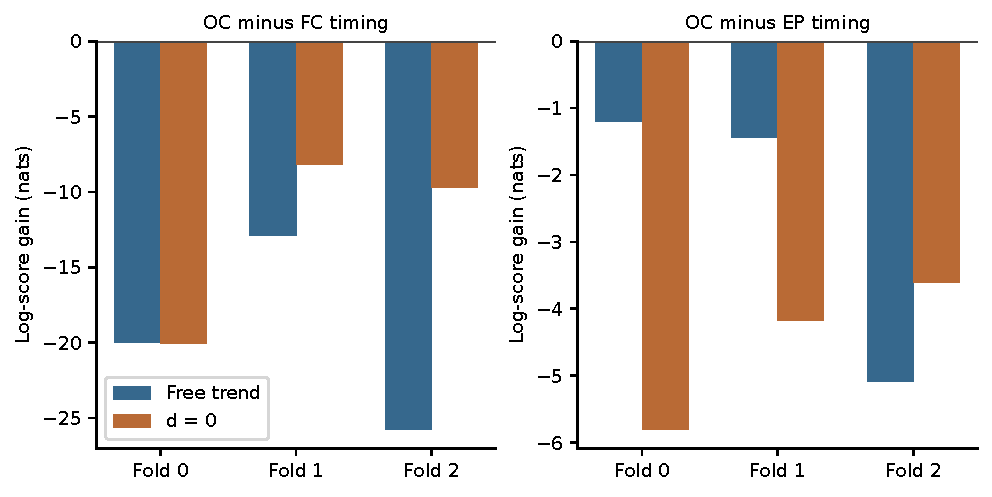
\includegraphics[width=\textwidth]{s06_jma_trend_timing.pdf}\caption{Saved JMA timing contrasts under free and stationary background trends. Each bar uses the same fold population; no new likelihood calculation or simulation was performed for the plot.}\end{figure}


\chapter{Conditional Simulation Diagnostics of Frozen Forecasts}
\label{ch:calibration}
\section{Conditional diagnostics: useful discrimination without overall adequacy}

\subsection{Frozen target and diagnostic reference}

The completed conditional check targets original frozen OC alone. For each of its three origins, 999 complete branching-future paths were generated conditional on that origin's fixed fitted state, nuisance choices and original prehistory. Descendants can generate further descendants. All 2,997 paths completed; failed and unknown counts are zero. They are dependent-event paths under the model, not 2,997 independent earthquake samples. The observed-path exposure is a realised predictable compensator; it is not a Poisson future-count mean.

Each origin has 84 recorded coordinates, covering count, time gaps and dependence, spatial transforms and allocation, scores and subblocks. The 252 entries are not 252 independent diagnostic tests: immigrant exposure is a deterministic bookkeeping coordinate at each fixed origin, and total-exposure and trigger-exposure ranks coincide because their difference is that fixed constant. Those entries are retained for accounting, explicitly flagged in Appendix~\ref{app:audit12}, and add no independent evidence of adequacy. The spatial transforms draw on the probability-integral-transform tradition \citep{Rosenblatt1952,Schoenberg2003}. A coordinate's insertion interval is

\begin{equation}
\left[\frac{1+\#\{S^{(r)}<S^{\rm obs}\}}{1000},\quad
\frac{1+\#\{S^{(r)}\leq S^{\rm obs}\}}{1000}\right].
\end{equation}

The resolution is 0.001. Boundary ranks are finite reference comparisons, not zero probability or exact population tail probabilities. Ties can create wide intervals. This descriptive collection has no asserted omnibus significance test, and its coordinates are not separate unadjusted discoveries. Empirical reference intervals describe simulated catalogues, not confidence intervals for fitted parameters or scientific validity.

\subsection{Discrepant and ordinary-looking results coexist}

\begingroup\footnotesize\setlength{\tabcolsep}{2pt}\renewcommand{\arraystretch}{1.18}
\begin{longtable}{@{}>{\raggedright\arraybackslash}p{0.1800\textwidth}>{\raggedright\arraybackslash}p{0.1800\textwidth}>{\raggedright\arraybackslash}p{0.1800\textwidth}>{\raggedright\arraybackslash}p{0.1800\textwidth}>{\raggedright\arraybackslash}p{0.1800\textwidth}@{}}
\toprule
{}Origin & Recorded count & Supplied simulated count interval & Count insertion interval & Selected diagnostic evidence \\
\midrule\endfirsthead
\toprule
Origin & Recorded count & Supplied simulated count interval & Count insertion interval & Selected diagnostic evidence \\
\midrule\endhead
\midrule\multicolumn{5}{r}{\emph{Continued on next page}}\\
\endfoot
\bottomrule\endlastfoot
{}Early & 79 & 121-453 & [0.001, 0.001] & Gap KS, serial statistic and spatial KS exceed every reference \\
{}Middle & 167 & 90-398 & [0.704, 0.712] & Ordinary total hides yearly concentration and dependence \\
{}Late & 69 & 69-279 & [0.021, 0.028] & Marginal gap/spatial KS ordinary; dependence and variance discrepant \\
\end{longtable}\endgroup

Early count is below all 999 simulated counts. Its exposure and trigger exposure are also below all references. Its gap KS is 0.222245 and spatial Rosenblatt KS is 0.167335, each above every reference. Yet the time event-logsum insertion is 0.583, the censored terminal tail 0.111 and within-cell absolute maximum 0.187. The model does not fail every coordinate in the same way.

Middle total count looks ordinary, but the five yearly counts are 12, 4, 8, 116 and 27. Its subblock balance maximum has insertion 0.998; the gap serial statistic exceeds all references. Its conditional-location score insertion is 0.364 and within-cell density score 0.312, while spatial KS, cross dependence and allocation show discrepancies. A satisfactory-looking total or score coordinate does not settle concentration or dependence.

Late gap KS has insertion 0.676 and spatial KS 0.810, yet serial dependence has insertion 0.998, the spatial cross statistic 0.992, and dimensionless location variance exceeds every reference. Across origins, cell 4 observed counts 15, 7 and 8 are below conditional allocations 23.493717, 16.132286 and 14.770085. These allocations sum conditional probabilities at observed event times; they are not unconditional event-count means. Empty-cell ties require particular care: one zero count has insertion [0.001, 0.563], which cannot be summarized by its lower endpoint.

Raw score totals also depend on target count and density measure. Early total location and joint scores exceed all simulated totals while its count is below all simulated counts; this does not validate its probabilities. Immigrant exposure ties identically across paths within a fixed state by construction. Neither that deterministic tie nor count-dependent mark totals validates the underlying recipe.

\subsection{Diagnostic scope}

OC shows material conditional diagnostic discrepancies in all three origins: early count and several dependence/spatial coordinates, middle concentration and dependence, and late dependence and location variance. The fixed-state forecast therefore lacks demonstrated conditional adequacy. That original coordinate-wise conclusion was descriptive rather than an omnibus rejection. EP was absent from that historical OC-only simulation experiment. The subsequent comparative conditional evaluation in Section~\ref{sec:s05-completed} includes EP and the declared within-origin omnibus statistics. Simulation-based forecast testing separates these questions \citep{Schorlemmer2007,Zechar2010}. Fitting, selection, measurement and catalogue-revision uncertainty are excluded by fixing the state. Later training histories include earlier target periods; separate per-origin simulations do not define a coherent cross-origin joint null. Cross-window patterns remain descriptive. Heavy-tailed productivity has infinite second moment under the fixed mark recipe, and normal/CLT count inference is not used. A censored terminal tail is survival information, not an additional completed gap.

The conditional diagnostic report and current evidence index retain the coordinate-level source and audit scope. All paths received identity/count/mark/exposure checks; independent full 84-coordinate raw replay covered nine paths, three prescribed indices per origin, not all 2,997 complete vectors. These are original audit outcomes. This edition recovered the simulation and diagnostic records and checked their hashes and source identities; it did not repeat that simulation or diagnostic campaign.



\section{Complete diagnostic record and subsequent evaluation}
Appendix~\ref{app:custody}, Section~\ref{app:audit12}, retains the complete coordinate tables and origin-specific rank figures, their reference definitions, and the independent numerical audit. The compact summary above and that full record describe the same frozen OC experiment.

The subsequent score-concentration and catalogue-robustness evaluation retained both discrepant and ordinary-looking diagnostics. Its completed results appear in Chapter~\ref{ch:external}; the frozen OC calibration target was not replaced by that follow-on.

\section{Completed conditional forecast calibration}

\label{sec:s05-completed}

Each model and California origin has 999 conditional simulated futures and its observed vector. The following tests condition on the fitted state and past history; they do not integrate parameter-estimation uncertainty.

\begin{table}[htbp]\centering\caption{Conditional count, original minimum-rank and continuous-coordinate pooled tests. All p-values use their declared inclusive-tail conventions.}\label{tab:s05-completed}

\begin{tabular}{llrrrr}\toprule Model & Fold & Conditional $N$ & Min-rank & Quadratic & Fisher-type\\\midrule

OC & 0 & 0.002 & 0.070 & 0.004 & 0.001 \\

OC & 1 & 0.594 & 0.075 & 0.003 & 0.004 \\

OC & 2 & 0.056 & 0.069 & 0.007 & 0.012 \\

EP & 0 & 0.002 & 0.070 & 0.004 & 0.002 \\

EP & 1 & 0.698 & 0.075 & 0.005 & 0.006 \\

EP & 2 & 0.036 & 0.069 & 0.009 & 0.008 \\

\bottomrule\end{tabular}\end{table}

The conditional count summary retains lower and upper inclusive empirical tails and reports twice the smaller tail, capped at one. The original minimum-rank test is retained with its exclusions and tie behaviour; it is not replaced by the continuous-coordinate statistics.

The pooled quadratic statistic uses eight declared coordinates: total exposure, time-event log sum, gap KS, gap serial correlation, spatial Rosenblatt KS maximum, absolute spatial cross-correlation, and dimensionless location-log-density mean and variance. Standardization and the ridge-regularized covariance are computed symmetrically on the observed vector plus all simulated vectors. The Fisher-type statistic is the preserved $-\sum_j\log\widetilde p_j$, not an independently calibrated chi-square reference or an assumption of independent coordinates. Both statistics use the inclusive upper rank in the same symmetric pool.

\begin{table}[htbp]\centering\caption{Retained-coordinate and tie diagnostics. Equal counts include the observed vector and every exactly tied pooled statistic.}

\begin{tabular}{llrrr}\toprule Model & Fold & Min-rank coordinates & Quadratic equal & Fisher equal\\\midrule

OC & 0 & 82 & 1 & 1 \\

OC & 1 & 82 & 1 & 1 \\

OC & 2 & 82 & 1 & 1 \\

EP & 0 & 82 & 1 & 1 \\

EP & 1 & 82 & 1 & 1 \\

EP & 2 & 82 & 1 & 1 \\

\bottomrule\end{tabular}\end{table}

Continuous does not automatically mean tie-free: coordinate duplicates and equality with the observed statistic are retained in the public aggregate and interpreted conservatively. This is the declared conditional calibration and pooled omnibus scope. No CSEP L-, M- or S-test results are inferred, and a non-rejection is not proof that the model or physical inhibition mechanism is correct. The independent reconstruction coverage is reported separately below; saved arithmetic checks and raw replay remain distinct forms of evidence.

\begin{figure}[htbp]\centering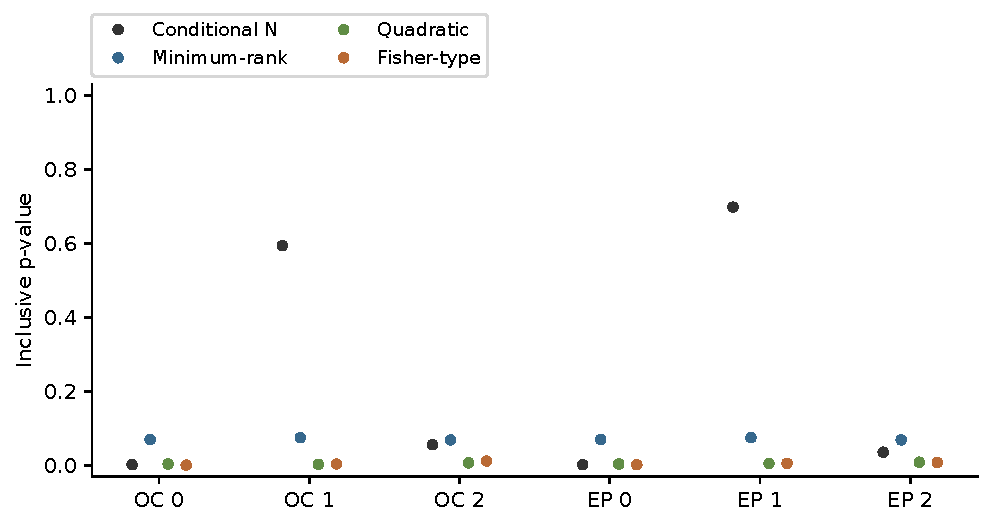
\includegraphics[width=\textwidth]{s05_conditional_pvalues.pdf}\caption{Reported inclusive conditional/pooled p-values.}\end{figure}

\begin{center}\begin{tabular}{llrrl}\toprule Model & Fold & Completed futures & Planned futures & Status\\\midrule

OC & 0 & 999 & 999 & resolved \\

OC & 1 & 999 & 999 & resolved \\

OC & 2 & 999 & 999 & resolved \\

EP & 0 & 999 & 999 & resolved \\

EP & 1 & 999 & 999 & resolved \\

EP & 2 & 999 & 999 & resolved \\

\bottomrule\end{tabular}\end{center}

Both continuous-statistic omnibus procedures reject at the declared five-percent level for each model and origin, while the retained minimum-rank procedure does not. Thus the EP score advantage is not a conditional-adequacy certificate. These are separate within-origin tests, not a joint cross-origin or model-selection-adjusted rejection. The historical OC full-vector audit remains separate.

% Additive replacement audit-scope text for 12_s05_completed.tex.
% Preserve every existing calibration p-value, table and figure.
The original completed independent closure reconstructed count, marks, immigrant and triggering exposure, temporal event logs, and spatial point, location and joint scores directly from all 5,994 saved OC and EP futures (999 per model and origin). It also reconstructed all 84 diagnostic coordinates and all 11 event-detail columns on EP indices 0, 249, 499, 749 and 998 in each of the three origins, giving 15 predeclared full-vector replays. Count identities are exact; finite numerical discrepancies satisfy the declared score, diagnostic and spatial-CDF tolerances. This extends the earlier nine-path native sample and zero-full-vector scope; it does not assert full spatial-PIT replay on all futures.

The independent reconstruction uses incomplete-beta line integrals and a separately implemented positive-polar rectangle-integration kernel. The scoring route and source identities are documented in \path{reproduction/regional/README.md}.

\begin{center}\begin{tabular}{lr}\toprule Independent closure quantity & Value\\\midrule
Independent raw point-score paths & 5994 \\
EP paths with all 84 diagnostics & 15 \\
Maximum point-score error (nats) & 1.17143e-09 \\
Maximum full-vector score error (nats) & 9.09495e-12 \\
Maximum other diagnostic error & 8.18545e-12 \\
Maximum spatial-CDF error & 6.66134e-15 \\
Maximum event-log error (nats) & 1.10134e-13 \\
Maximum gap error & 1.15463e-14 \\
\bottomrule\end{tabular}\end{center}



\chapter{Continuous Immigrant Local Inhibition and Synthetic Control Regimes}
\label{ch:local-inhibition}
\section{Study overview}

The registered continuous local-inhibition (LI) procedure selects exactly zero inhibition strength in all three previously inspected California test windows. Across the same 315 targets used in the preceding comparisons, LI is a numerical tie with matched Omori continuous (OC); its raw pooled positive difference is only 1.884928e-10 total nats and is not a predictive gain. The inverse-power ETAS benchmark (EP) remains better jointly in every window, mainly through conditional location. In the historical initial control study, all eight fixed-seed controls are retained: LI loses to OC on both uniform-null, both smooth-null and both narrow/short-inhibition datasets, and wins on both broad/long-inhibition datasets. Two seeds per regime cannot estimate power or a false-positive rate, and the narrow/short losses prevent a claim that this procedure would reliably detect inhibition when present. At zero inhibition, range and memory are unidentified. These results concern a frozen statistical extension that attenuates only the immigrant component at recorded coordinates; they do not establish absence of physical inhibition, causal mechanisms, significance or global optimization.

\section{Key question and review status}

Does spatially local, temporary attenuation improve retrospective prediction beyond the matched OC procedure, and does the resulting procedure compete with EP? The question follows the positive continuous-location ablation in Chapter~\ref{ch:nz-spatial} and the more qualified external, benchmark and diagnostic findings in Chapter~\ref{ch:external}. It requires an actual likelihood with full exposure, a frozen fitting rule, matched references, retained negative controls and complete accounting. A term described as inhibition is not evidence that a physical stress-depletion mechanism has been identified.

The historical source is the accepted initial local-inhibition completion, including its selected-state diagnostics, aggregate checker and preservation audits. Its results remain identified separately from the expanded controls in Section~\ref{sec:s04-expanded}, which report new numerical follow-up. The historical source authorities remain unchanged. It activates no live forecast. Underlying independent computational review is distinct from external academic inspection; the latter remains pending for this package.

\section{Recorded-event design and comparator definitions}

\subsection{Same California history, not a new sample}

The observation law selects preferred California records with reported M $\geq$ 4.0, latitude 32-37 degrees, longitude -121 to -114 degrees and depth -5 to 40 km. The fixed source contains 1,272 unique events: 106 warmup parents in 1981-1985 and 1,166 evaluated records in 1986-2026. The latter comprise 851 initial training targets plus 315 subsequent test targets. Warmup is already included in 1,272; the counts must not be added a second time.

\begingroup\footnotesize\setlength{\tabcolsep}{2pt}\renewcommand{\arraystretch}{1.18}
\begin{longtable}{@{}>{\raggedright\arraybackslash}p{0.1800\textwidth}>{\raggedright\arraybackslash}p{0.1800\textwidth}>{\raggedright\arraybackslash}p{0.1800\textwidth}>{\raggedright\arraybackslash}p{0.1800\textwidth}>{\raggedright\arraybackslash}p{0.1800\textwidth}@{}}
\toprule
{}Fold & Test window, UTC & Training targets & Test targets & Exposure days \\
\midrule\endfirsthead
\toprule
Fold & Test window, UTC & Training targets & Test targets & Exposure days \\
\midrule\endhead
\midrule\multicolumn{5}{r}{\emph{Continued on next page}}\\
\endfoot
\bottomrule\endlastfoot
{}F0 & 2011-2016 & 851 & 79 & 1,826 \\
{}F1 & 2016-2021 & 930 & 167 & 1,827 \\
{}F2 & 2021-2026 & 1,097 & 69 & 1,826 \\
{}Pooled test & 2011-2026 & Overlapping prefixes & 315 & 5,479 \\
\end{longtable}\endgroup

These are the same 315 targets in the California replication, benchmark, conditional diagnostic and concentration studies. Their repeated evaluation is not independent replication. The archive and earlier annual/sequence outcomes had already been inspected. Parameters and nuisance choices use training data, remain frozen in test, and histories update sequentially after each observed timestamp. Only strictly earlier eligible events enter excitation and inhibition; timestamp ties are processed as a batch, with no within-batch self- or mutual influence.

\subsection{The references answer different questions}

OC means Omori temporal triggering with the finite-domain continuous, reference-density-weighted offspring law and smooth immigrant background. EP means a separately fitted Omori ETAS adaptation whose inverse-power radial offspring density is normalized directly against projected area without OC's reference weighting. EP is an excitation model, not a Poisson model. LI-OC is the matched extension comparison. LI-EP compares complete competing procedures with different spatial excitation laws and does not isolate inhibition alone.

For completeness, the other abbreviations in the programme are FC (fixed-scale Mittag-Leffler continuous), FL (its cell-lift counterpart), OL (Omori cell-lift), MC (free common-scale Mittag-Leffler continuous) and N0 (a separately refitted smooth no-trigger procedure). Their primary contrasts are detailed in Chapter~\ref{ch:external}. A constant-Poisson candidate here is a numerical optimization floor, distinct from N0 and EP.

\section{The continuous immigrant-inhibition model}

\subsection{Intensity and attenuation field}

For time t and recorded projected location z in the fixed finite domain D, the model is

\begin{align}
\lambda_{\rm LI}(t,z)&=e^{a+dx_{\mathrm{trend}}(t)}b_{\rm bg}(z)e^{-\eta G(t,z)}+nH_{\rm OC}(t,z),\label{eq:spatial-li-intensity}\\
x_{\mathrm{trend}}(t)&=2t/T_0-1,\qquad T_0=16436\ \text{days},\\
G(t,z)&=\sum_{j:t_j<t}e^{-(t-t_j)/\psi}
\left(1+\frac{\lVert z-z_j\rVert^2}{\ell^2}\right)^{-2}.\label{eq:spatial-li-field}
\end{align}
The observed clock is days since 1981-01-01 00:00:00 UTC.

Here $a$ and $d$ govern immigrant amplitude/trend; $b_{\rm bg}$ is the inherited training-only background density; $n$ scales excitation $H_{\rm OC}$; $\eta$ is nonnegative inhibition strength; $\ell$ is its spatial range in kilometres; and $\psi$ is its memory in days. The observed clock uses the frozen timestamp convention and strict earlier-integer-timestamp parent rule, including tied batches. Synthetic controls have their own day-zero origin and normalization, specified in Section~\ref{sec:li-generating-contract}. The stress mark multiplier is fixed to one: every eligible earlier recorded event contributes to $G$ without magnitude weighting. No latent immigrant/offspring classification is required. Inhibition acts only on the immigrant term. It does not suppress $H_{\rm OC}$, and it is not spatially renormalized. It therefore changes both local density and total immigrant rate. Renormalizing the inhibited density would define a different model.

The unit stress mark is a substantive restriction: at the same lag and separation, an eligible M4 event and an eligible M7.1 event contribute equally to the attenuation field. Their excitation productivity can still differ through $\kappa_j$. This model therefore does not represent magnitude-scaled stress release, a Coulomb stress tensor, or suppression of the full triggered sequence. It tests immigrant attenuation under one restricted statistical law.

More explicitly, the inherited excitation is a sum over all eligible strictly earlier parents:

\begin{align}
H_{\rm OC}(t,z)&=\sum_{j:t_j<t}\kappa_j k_O(t-t_j)s_\sigma(z\mid z_j),\\
k_O(u)&=\frac{(p-1)c^{p-1}}{(u+c)^p},\qquad u>0,\\
s_\sigma(z\mid z_j)&=\frac{b_{\rm ref}(z)(1+\lVert z-z_j\rVert^2/\sigma^2)^{-2}}{Z_j},\label{eq:spatial-normalized-density}\\
Z_j&=\int_D b_{\rm ref}(v)(1+\lVert v-z_j\rVert^2/\sigma^2)^{-2}\,\mathrm dv.
\end{align}

Here $\kappa_j$ is the shared training-calibrated magnitude-productivity weight, with fixed exponent $r=0.7$; $b_{\rm ref}$ is the frozen training-derived reference geography. The background $b_{\rm bg}$ integrates to one on $D$. The temporal kernel integrates to one over all positive lags and each $s_\sigma$ integrates to one on $D$; exposures use the actual finite time window. The training-only smooth background, parent eligibility and inherited excitation nuisance choices follow the matched OC procedure. LI introduces no new background bandwidth or excitation spatial-scale search. The stress radial factor in $G$ itself is not a normalized spatial probability density; it is an attenuation field inside the exponential.

The temporal factor is the normalized Omori--Utsu law \citep{Utsu1995}; the reference-weighted spatial factor is a particular fitted forecasting choice rather than a physical stress law.

At $\eta$ = 0, $\exp[-\eta G]$ equals one everywhere and LI exactly nests OC when shared coordinates agree. All $\ell$ and $\psi$ choices then give the same law. Canonical $\ell$ = 30 km and $\psi$ = 7 days are display conventions at that boundary, not recovered scales. Even a positive procedure score difference at $\eta$ = 0 could arise from refitting shared coordinates through another optimization path; it would not establish active attenuation. The separate approved selected-state diagnostics are therefore essential to the conclusion below.

\subsection{Frozen fitting and selection contract}

The fitted coordinates are $(a,d,n,\log c,p,\eta,\log\ell,\log\psi)$, where $c$ and $p$ parameterize the normalized Omori kernel. The physical bounds are fixed.

\begingroup\small\setlength{\tabcolsep}{2pt}\renewcommand{\arraystretch}{1.18}
\begin{longtable}{@{}>{\raggedright\arraybackslash}p{0.2280\textwidth}>{\raggedright\arraybackslash}p{0.2280\textwidth}>{\raggedright\arraybackslash}p{0.2280\textwidth}>{\raggedright\arraybackslash}p{0.2280\textwidth}@{}}
\toprule
{}Coordinate & Bound & Coordinate & Bound \\
\midrule\endfirsthead
\toprule
Coordinate & Bound & Coordinate & Bound \\
\midrule\endhead
\midrule\multicolumn{4}{r}{\emph{Continued on next page}}\\
\endfoot
\bottomrule\endlastfoot
{}a & [-12, 0] & d & [-2, 2] \\
{}n & [0, 0.98] & c & [0.0001, 20] days \\
{}p & [1.01, 2.5] & $\eta$ & [0, 4] \\
{}$\ell$ & [5, 150] km & $\psi$ & [1/24, 365] days \\
\end{longtable}\endgroup

Each main arm has eight prescribed starts. For LI fits only, shared a,d,n start from the accepted matched OC state. LI start 0 retains OC's c,p and $\eta$ = 0; the other LI starts use the fixed c,p,$\eta$,$\ell$,$\psi$ schedule below. Synthetic OC control fits use a separate frozen initialization rule, not their own subsequently accepted fit: a0 = clip(log(0.6 max(Ntrain,1)/365), -11.5, -0.1), d0 = 0.2 and n0 = 0.35, with eight prescribed c,p rows in synthetic\_\allowbreak{}common/OC\_\allowbreak{}start\_\allowbreak{}fill. The readable protocol subset gives both start schemes, floors, bounds and tolerances in full.

L-BFGS-B has maxiter 200, maxfun 20,000, maxls 200, ftol 1e-10 and gtol 2e-6. Bounded Powell is allowed only after failure of the declared first-method acceptance rule, from the same original start, with maxiter 400, maxfev 5,000, xtol 1e-6 and ftol 1e-10. These limits describe a bounded search, not a global optimization proof.

\begingroup\small\setlength{\tabcolsep}{2pt}\renewcommand{\arraystretch}{1.18}
\begin{longtable}{@{}>{\raggedright\arraybackslash}p{0.2280\textwidth}>{\raggedright\arraybackslash}p{0.2280\textwidth}>{\raggedright\arraybackslash}p{0.2280\textwidth}>{\raggedright\arraybackslash}p{0.2280\textwidth}@{}}
\toprule
{}LI start: c (days), p & $\eta$ & $\ell$ (km) & $\psi$ (days) \\
\midrule\endfirsthead
\toprule
LI start: c (days), p & $\eta$ & $\ell$ (km) & $\psi$ (days) \\
\midrule\endhead
\midrule\multicolumn{4}{r}{\emph{Continued on next page}}\\
\endfoot
\bottomrule\endlastfoot
{}0: accepted OC c,p & 0 & 30 & 7 \\
{}1: 0.0001, 1.1 & 0.1 & 5 & 1/24 \\
{}2: 0.001, 1.3 & 0.3 & 15 & 0.25 \\
{}3: 0.01, 1.1 & 0.7 & 50 & 7 \\
{}4: 0.1, 1.3 & 1.5 & 150 & 30 \\
{}5: 1, 1.7 & 3 & 5 & 365 \\
{}6: 20, 2.5 & 4 & 150 & 1/24 \\
{}7: 0.1, 1.01 & 0.5 & 30 & 365 \\
\end{longtable}\endgroup

Selection minimizes accepted training joint negative log likelihood. Exact ties prefer the OC floor, then the Poisson floor, then start and method ordinals. Held-out score does not select a candidate, method, computational epoch or seed. Candidates within 0.0004 training NLL units of the selected state receive the declared held-out spread check, requiring spread strictly below 0.01 nats per target. This is an admission/sensitivity diagnostic over the stored near-optimal set; it is neither an uncertainty interval nor permission to select the best test forecast.

The readable protocol subset and exact data-free case matrix copy expose the full start schedules, law, observation scope and selection rule; source pins bind their identities. The case matrix retains historical execution-status labels; final accepted completion receipts establish the results status. An earlier methods proposal is contextual, and the structured frozen case matrix is authoritative where it differs.

\subsection{Proper scores and exposure}

Write P for summed event log point intensity, Q for summed event log regional intensity, E for positive full-domain integrated intensity, C = -E for its signed score contribution and M for the common magnitude-mark score. Then

\begin{align}
S_{\rm time}&=Q+C=Q-E,&S_{\rm loc}&=P-Q,\\
S_{\rm joint}&=P+C+M=S_{\rm time}+S_{\rm loc}+M,\\
\Delta P&=P_{\rm LI}-P_R,&\Delta C&=E_R-E_{\rm LI},\\
\Delta S_{\rm joint}&=\Delta P+\Delta C+\Delta M.
\end{align}

All quiet-period and full-domain exposure is retained. Lower exposure can offset a worse event-intensity term; an event-only gain is insufficient. Within each arm, Q uses that arm's spatially integrated ground intensity under the fixed observed history, and all components use its same fitted state. Independently fitted arms can have different parameters. The shared conditional mark law is scored once and cancels in contrasts. Pooled scores sum all three window totals and divide by 315. These are nats of realised predictive log score, not percent accuracy, correlation, a physical effect size or evidence of calibration.

The source-field dictionary distinguishes these narrative symbols from legacy aggregate keys. In particular, LI's raw pooled E field means the point-event logsum difference, not positive exposure; its raw C is the signed exposure contribution. Sequence timing\_\allowbreak{}compensator instead stores signed difference in nonnegative integrated exposure and enters the score negatively. Source keys and scalars remain unchanged.

\section{Observed result: no selected inhibition and a numerical tie}

All three selected LI fits have $\eta$ \textbf{exactly zero}. The procedure selects no active attenuation term in these observed windows. Its joint contrasts against OC are numerical ties under the frozen aggregate sign tolerance of +/-0.0002 total nats (inclusive).

\begingroup\footnotesize\setlength{\tabcolsep}{2pt}\renewcommand{\arraystretch}{1.18}
\begin{longtable}{@{}>{\raggedright\arraybackslash}p{0.1800\textwidth}>{\raggedright\arraybackslash}p{0.1800\textwidth}>{\raggedright\arraybackslash}p{0.1800\textwidth}>{\raggedright\arraybackslash}p{0.1800\textwidth}>{\raggedright\arraybackslash}p{0.1800\textwidth}@{}}
\toprule
{}Window & Targets & LI-OC joint nats/target & Selected $\eta$ & Interpretation \\
\midrule\endfirsthead
\toprule
Window & Targets & LI-OC joint nats/target & Selected $\eta$ & Interpretation \\
\midrule\endhead
\midrule\multicolumn{5}{r}{\emph{Continued on next page}}\\
\endfoot
\bottomrule\endlastfoot
{}F0 & 79 & 0 & 0 & Numerical tie \\
{}F1 & 167 & +1.128699e-12 & 0 & Numerical tie \\
{}F2 & 69 & 0 & 0 & Numerical tie \\
{}Pooled & 315 & +5.983898e-13 & 0 in 3/3 & Numerical tie \\
\end{longtable}\endgroup

The raw pooled difference is +1.88492776942439e-10 total nats. Its tiny positive floating-point sign is retained for arithmetic traceability and is not a forecast improvement. The frozen aggregate sign tolerance concerns numerical comparison, not statistical significance or a fitter admission gate. Exact model nesting and finite arithmetic are separate issues: the selected law has no inhibition, while independently evaluated saved score arithmetic may differ at roundoff scale.

The zero-strength boundary leaves $\ell$ and $\psi$ unidentified. Neither their canonical values nor bounds identify a physical inhibition footprint or duration. This result supports the narrower statement that the registered fitting procedure selected no active immigrant attenuation on this inspected recorded-coordinate history. It supplies no proof that earthquakes lack inhibition, no universal detection limit and no evidence of physical absence.

\section{EP remains the stronger joint forecast}

LI scores below EP in every observed window. Its pooled timing edge is tiny and mixed across windows; its larger conditional-location deficit accounts for the joint loss. All differences below are LI minus EP in nats per target.

\begingroup\footnotesize\setlength{\tabcolsep}{2pt}\renewcommand{\arraystretch}{1.18}
\begin{longtable}{@{}>{\raggedright\arraybackslash}p{0.1800\textwidth}>{\raggedright\arraybackslash}p{0.1800\textwidth}>{\raggedright\arraybackslash}p{0.1800\textwidth}>{\raggedright\arraybackslash}p{0.1800\textwidth}>{\raggedright\arraybackslash}p{0.1800\textwidth}@{}}
\toprule
{}Window (targets) & Timing & Conditional location & Joint & Mark difference \\
\midrule\endfirsthead
\toprule
Window (targets) & Timing & Conditional location & Joint & Mark difference \\
\midrule\endhead
\midrule\multicolumn{5}{r}{\emph{Continued on next page}}\\
\endfoot
\bottomrule\endlastfoot
{}F0 (79) & +0.006244055 & -0.085849360 & -0.079605305 & 0 \\
{}F1 (167) & -0.001101051 & -0.188973874 & -0.190074925 & 0 \\
{}F2 (69) & +0.000389054 & -0.189082869 & -0.188693815 & 0 \\
{}Pooled (315) & +0.00106746 & -0.163135 & -0.162067 & 0 \\
\end{longtable}\endgroup

The exact source-reported pooled LI-EP joint difference is -51.0512047628713 total nats, or -0.162067316707528 per target. Its timing and conditional-location totals are +0.336249525419333 and -51.3874542882905. These are predictive components, not causal shares or a decomposition of physical immigrant versus offspring generation.

The separately archived OC-EP benchmark in IV differs slightly at floating-point scale from this replay. Each is reported under its own accepted source identity; substituting one for the other would obscure provenance. Neither EP's better relative score nor LI's exact nesting supplies a probability-calibration result. The completed conditional calibration concerned original OC only and found material discrepancies.

\section{Every fixed-seed control, including the failures}

\subsection{Generating contract}\label{sec:li-generating-contract}

Eight datasets, two seeds per regime, were fixed in advance. The null regimes have $\eta$ = 0. The narrow/short positive regime has $\eta$ = 0.5, $\ell$ = 5 km and $\psi$ = 1/24 day. The broad/long regime has $\eta$ = 2, $\ell$ = 50 km and $\psi$ = 30 days. At the null, $\ell$/$\psi$ do not affect the law. The domain is 100 by 100 km; synthetic t is days since simulated history begins at day zero, with $x_{\mathrm{trend}}(t)=2t/760-1$. Warmup ends at day 30, training at day 395 and test at day 760. The observed 16,436-day normalization is not used for these controls. Known nuisance/background inputs are fixed equally for paired OC/LI fits. Chronological thinning uses accepted-event ancestry and fixed PCG64DXSM streams, with original caps/failures attached to their seeds. No failed or inconvenient seed is redrawn.

The controls test the registered fitting procedure on these laws. They do not mimic every catalogue feature, location-error process or earthquake mechanism. The public control table is complete.

\begingroup\footnotesize\setlength{\tabcolsep}{2pt}\renewcommand{\arraystretch}{1.18}
\begin{longtable}{@{}>{\raggedright\arraybackslash}p{0.1800\textwidth}>{\raggedright\arraybackslash}p{0.1800\textwidth}>{\raggedright\arraybackslash}p{0.1800\textwidth}>{\raggedright\arraybackslash}p{0.1800\textwidth}>{\raggedright\arraybackslash}p{0.1800\textwidth}@{}}
\toprule
{}Generating regime & Seed & Test targets & LI-OC joint nats & Nats/target \\
\midrule\endfirsthead
\toprule
Generating regime & Seed & Test targets & LI-OC joint nats & Nats/target \\
\midrule\endhead
\midrule\multicolumn{5}{r}{\emph{Continued on next page}}\\
\endfoot
\bottomrule\endlastfoot
{}Uniform null & 410001 & 116 & -148.647608 & -1.281445 \\
{}Uniform null & 410002 & 138 & -4.930159 & -0.035726 \\
{}Smooth null & 410101 & 128 & -4.489917 & -0.035077 \\
{}Smooth null & 410102 & 120 & -7.638775 & -0.063656 \\
{}Narrow/short inhibition & 410201 & 107 & -1.297391 & -0.012125 \\
{}Narrow/short inhibition & 410202 & 102 & -25.357970 & -0.248608 \\
{}Broad/long inhibition & 410301 & 23 & +2.242679 & +0.097508 \\
{}Broad/long inhibition & 410302 & 27 & +6.771012 & +0.250778 \\
\end{longtable}\endgroup

LI loses on six examples, including both positive narrow/short laws, and wins on the two broad/long examples. The first uniform-null loss is large and remains displayed. The broad/long examples contain only 23 and 27 test targets. Averaging these rows into a single success rate would discard the intentionally different laws and denominators.

These controls do not establish reliable recovery even within the tested positive-inhibition family. They are compatible with finite-sample overfitting, weak information about the extra coordinates, or limitations of the bounded numerical search; two seeds per regime do not distinguish those explanations. In particular, a nested training floor at $\eta=0$ protects training likelihood, not future log score. A large held-out loss therefore does not by itself prove optimizer failure. The LI initialization uses the accepted fitted OC state, not a guarantee that all starting coordinates equal the generating truth. The two broad/long wins do not establish general power, and the null losses do not identify a physical mechanism.

\clearpage
\begin{figure}[p]\centering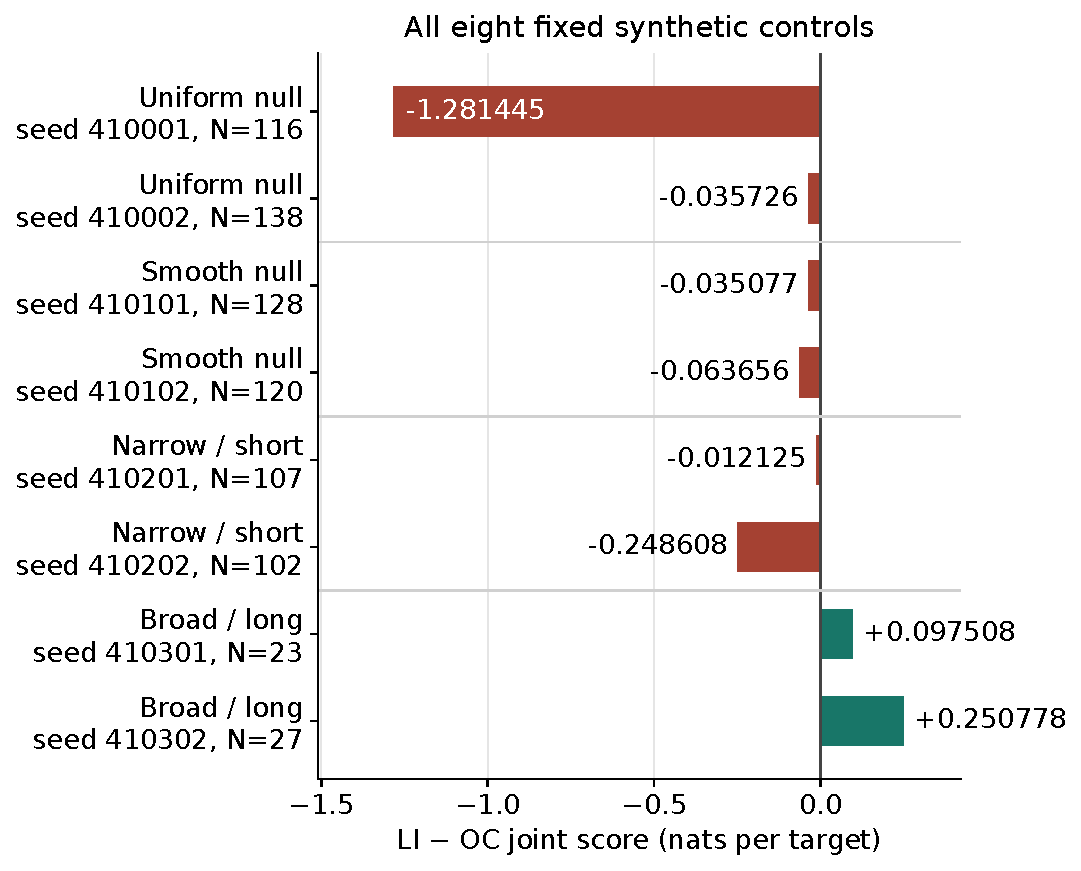
\includegraphics[width=\linewidth,height=.78\textheight,keepaspectratio]{spatial_addendum_v_li_fixed_controls.pdf}
\caption{All eight prescribed LI-minus-OC fixed controls. The full linear scale retains the large uniform-null loss. Every seed and test count remains labelled. Positive means LI scored better; the rows are fixed examples, not estimated success probabilities.}\end{figure}
\clearpage



\subsection{What the controls do and do not show}

Both broad/long wins show that the registered procedure can improve held-out score on those two fixed examples. Both narrow/short losses show why the observed zero-strength result cannot be read as a reliable absence test. A true positive term in the generating law need not improve this finite-sample fitted procedure's held-out score. Conversely, an active fitted term or better score would not identify a physical mechanism.

Two seeds per regime cannot estimate false-positive rate, power, parameter coverage or general recovery probability. Six losses do not prove absence of inhibition in the generating laws, and two wins do not establish reliable detection. Narrow/short failure does not locate a physical resolution threshold. The recorded-coordinate law has no admitted empirical location-error distribution; the engineering lower bound $\ell$ = 5 km is a model/search constraint, not a measurement-accuracy assertion.

\section{Identifiability and consolidated scientific implications}

At $\eta$ = 0 the likelihood does not depend on $\ell$ or $\psi$. Thus zero-strength selection does not estimate a zero range or duration: it removes those coordinates from the law. The null also lies at the boundary of a constrained parameter space. Exact nesting alone justifies neither ordinary Wilks inference nor a universal half-chi-square reference. No significance, p-value or event-iid confidence interval is reported.

The finite multistart procedure is part of the estimand. Negative held-out differences are possible even for nested model families because training-defined selection and finite samples do not guarantee held-out superiority. The complete retained candidates and near-optimal checks reduce particular numerical concerns; they do not certify a global optimum or prove that no positive-inhibition state could ever perform better. The conclusion must stay about the registered procedure and this history.

Together with Chapter~\ref{ch:external}, the programme supports a qualified predictive conclusion. Continuous offspring geography improves location relative to the declared cell-lift procedure in the examined regional comparisons. Omori's timing advantage is conditional and reverses in Japan. OC and its zero-inhibition LI extension remain below EP jointly in California; EP also wins in Japan. OC and EP both show fixed-state conditional discrepancies in Section~\ref{sec:s05-completed}; prospective calibration remains separate. California score gains are heterogeneous and concentrated in a single eligible scored sequence period while retaining positive contextual totals over the complete complement.

The new LI result adds a negative extension finding: no selected active inhibition and no predictive gain over matched OC in the observed windows. It does not overturn the earlier location ablation, reverse the serious-benchmark deficit, resolve calibration, recover physical labels or prove absence of a physical mechanism. The eight controls reinforce the need to distinguish procedural sensitivity from a physical absence claim.

All archives had been inspected and revised. Chronological test windows are related through overlapping training history and earthquake dependence, and the same California targets recur across studies. No pristine confirmation, broad independent sequence replication or causal conclusion follows. The prospective New Zealand programme remains readiness only; future capture, issuance and scoring are separate from these historical results. This chapter provides no issued-forecast outcomes, scheduling activation or publication decision.

\section{Numerical completion is a separate validation result}

The historical initial completed roster contains 19 fit procedures: paired OC/LI fits for eight synthetic datasets plus three observed LI fits. It accounts for 152 prescribed starts and 30 floors, giving 182 final slots. Seventeen historical CPU fits were preserved; the two remaining observed fits completed with the admitted GPU provider. Nineteen score jobs replayed all candidates and finite feasible solver returns. These are computation denominators, not 19 empirical replications.

The 42 validation jobs comprise 38 procedure-phase audits, three paired sealed-reference jobs covering six comparator states, and a separate censored-attempt preservation audit. The earlier interrupted LI pool remains excluded from the final eligible pool and preserved separately; its partial success did not select the final computational epoch. Recovery changed execution machinery within the frozen scientific law and roster. No observed event was removed and no synthetic seed was replaced.

All 19 training-defined near-optimal spreads are below 0.01 nats per target; the largest is 0.00053761640079144. The exact aggregate checker passed 369 checks, with independent saved-output review and arithmetic reconstruction. Gradient statuses are fully accounted for. These checks support custody and numerical consistency under tested states, not universal gradient representability, scientific replication, physical scale recovery or global optimization.

\section{Evidence and reading guide}

The accepted scientific report is the source for observed results, all controls and completion counts. The computational provenance report preserves execution/recovery boundaries. The current evidence index routes the unchanged aggregate, source pins, complete claim bindings and field semantics. The evidence catalogue, readable protocol subset and review guide supply the exact source identities, full scientific contract and inspection order.

Claim families LI-OBSERVED, LI-CONTROLS and LI-VALIDATION separate the scientific result, fixed examples and numerical evidence. CA-BENCHMARK and CA-CALIBRATION supply the earlier comparator/calibration context; OPS-READINESS supplies the separate future-operations boundary. Current figure arithmetic is reproduced from accepted scalars; underlying fits, simulations and audits remain source-reported. Raw records, event caches and fitted vectors remain outside the review bundle. External scientific inspection is pending.

\section{Expanded fixed-backbone controls and magnitude-scaled inhibition}

\label{sec:s04-expanded}

The original S04 completed campaign expands the fixed-seed control matrix and evaluates magnitude-scaled immigrant-only and total-intensity inhibition (LI+). The earlier eight examples above remain historical results under their original numerical procedure. The expanded results below use the same declared generating regimes and shared fixed background/excitation inputs; they are not full joint nuisance refits.

The original S04 positive-control histories are generated by the original unit-mark, immigrant-only LI law. Magnitude-scaled LI+ and total-intensity attenuation are alternative fitted procedures on those same histories, not their matched generating models. Their contrast therefore measures performance under that specified generator; it does not establish relative power when magnitude-scaled or total-intensity inhibition generates the data.

The original S04 expanded roster contains 80 distinct histories, 20 in each regime, with five paired procedure/gate combinations and 400 score rows. The stress field is
\[
G_+(t,z)=\sum_{t_j<t}\exp\{\gamma Q_j-(t-t_j)/\psi\}
 \left(1+\|z-z_j\|^2/\ell^2\right)^{-2},\qquad
\gamma=\tfrac34\log 10.
\]
Here $Q_j$ is excess magnitude, so the reference excess is zero. Original LI uses the same field with unit magnitude weights. This bounded design retains a common shadow radius; it does not fit a magnitude-dependent rupture radius. With the shared fixed backbone written $B+nH$, the two LI+ intensities are
\[
 \lambda_{\rm imm}=B e^{-\eta G_+}+nH,
 \qquad \lambda_{\rm total}=(B+nH)e^{-\eta G_+}.
\]
The gate retains an active fit only when its training log-likelihood improvement exceeds $\tfrac32\log N_{\rm train}$.

The BIC-style gate is a training-only complexity penalty, not a Davies-calibrated test or a nominal-size guarantee. The gate can select the exact uninhibited floor. A held-out win and an active training fit are distinct outcomes. No seed was redrawn and no negative score was removed.

\begingroup\footnotesize\setlength{\tabcolsep}{3pt}

\begin{longtable}{@{}llrrrrr@{}}

\toprule Regime & Procedure & $N$ & Mean gain & MC SE & Median & Wins \\

\midrule\endfirsthead

\toprule Regime & Procedure & $N$ & Mean gain & MC SE & Median & Wins \\

\midrule\endhead

\bottomrule\endlastfoot

Uniform null & LI & 20 & -2.9299 & 0.9259 & -1.6435 & 3 \\

Uniform null & LI+ immigrant gated & 20 & 0.0000 & 0.0000 & 0.0000 & 0 \\

Uniform null & LI+ immigrant & 20 & -2.9514 & 1.3451 & -0.3835 & 4 \\

Uniform null & LI+ total gated & 20 & 0.0000 & 0.0000 & 0.0000 & 0 \\

Uniform null & LI+ total & 20 & -74.6499 & 42.9783 & -2.2181 & 1 \\

Smooth null & LI & 20 & -3.4230 & 1.3263 & -2.2716 & 4 \\

Smooth null & LI+ immigrant gated & 20 & 0.0000 & 0.0000 & 0.0000 & 0 \\

Smooth null & LI+ immigrant & 20 & -3.6408 & 1.5156 & -1.9787 & 4 \\

Smooth null & LI+ total gated & 20 & 0.0000 & 0.0000 & 0.0000 & 0 \\

Smooth null & LI+ total & 20 & -448.5272 & 445.0217 & -0.0604 & 3 \\

Narrow/short & LI & 20 & -3.8713 & 1.3147 & -2.3528 & 3 \\

Narrow/short & LI+ immigrant gated & 20 & 0.0000 & 0.0000 & 0.0000 & 0 \\

Narrow/short & LI+ immigrant & 20 & -3.4720 & 1.6063 & -1.1309 & 4 \\

Narrow/short & LI+ total gated & 20 & 0.0000 & 0.0000 & 0.0000 & 0 \\

Narrow/short & LI+ total & 20 & -129.3344 & 103.6071 & -0.6334 & 6 \\

Broad/long & LI & 20 & 33.8922 & 1.2083 & 33.4049 & 20 \\

Broad/long & LI+ immigrant gated & 20 & 28.3296 & 1.6682 & 26.6651 & 20 \\

Broad/long & LI+ immigrant & 20 & 28.3296 & 1.6682 & 26.6651 & 20 \\

Broad/long & LI+ total gated & 20 & -5.4013 & 13.7572 & 3.9231 & 10 \\

Broad/long & LI+ total & 20 & -5.3446 & 13.7585 & 4.4063 & 14 \\

\end{longtable}\endgroup

Mean and median gains are total held-out log-score differences from the shared uninhibited baseline; MC SE is the sample standard deviation divided by the square root of the number of independent seeded datasets within each regime. It is a descriptive finite-sample summary, not a calibrated confidence interval. The unbounded magnitude transforms and large retained losses do not by themselves establish finite score variance or a Gaussian approximation. The broad/long regime supports improved mean performance for original LI and immigrant-only LI+. Total-intensity attenuation has a negative mean even there, despite a positive median. The large negative means in other regimes are retained rather than trimmed.

In original S04, gating selects the uninhibited floor throughout both null regimes, but also throughout the narrow/short positive regime. This demonstrates the sensitivity--overfitting tradeoff of this procedure on these controls; it does not establish nominal Type I error or general detection power.

The original S04 completed matrix combines accepted first-pass results with quadrature refinement and same-history finer-grid refits. Training-only selection preserves the prescribed starts, bounds and exact uninhibited floor. Finer-grid validation checks retained candidates, score decomposition and forecast spread. Independent compiled CPU replays cover predeclared anchors; the remaining cases have per-case numerical checks and sampled-audit coverage, not individual independent replay. All aggregate tables and their source identities are retained in the evidence bundle.

These results extend the synthetic evidence only. They do not replace the observed California comparison, for which the completed observed LI+ evaluation is reported in Section~\ref{sec:s04-observed-completed} below.

\begin{figure}[p]\centering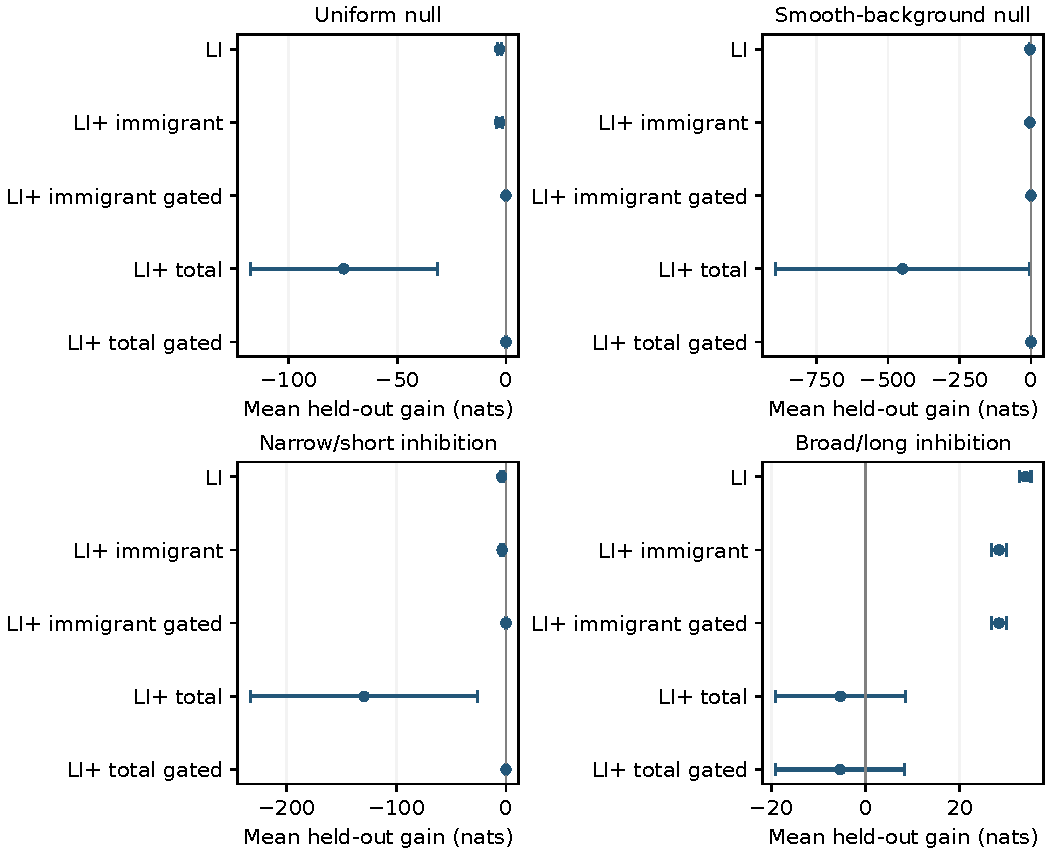
\includegraphics[width=\linewidth]{s04_unitmark_mean_gains.pdf}
\caption{Original S04 unit-mark fixed-backbone controls. Points show mean held-out gain and bars show the descriptive sample standard deviation divided by the square root of the row denominator, labelled MC SE in the table. These bars are not calibrated confidence intervals. Panels retain their full linear ranges, including large losses; horizontal scales differ. Each plotted summary uses the full corresponding row denominator in the preceding table. The zero line is the shared uninhibited comparator.}\end{figure}


\subsection{Matched magnitude-scaled generators (S04B)}

\label{sec:s04b-matched}

S04B is a separate matched-generator extension, not a replacement for the unit-mark S04 controls above. Magnitude-scaled immigrant-only and total-intensity laws each generate narrow/short and broad/long positive controls. Only accepted events enter the strictly prior stress field and spawn descendants. Immigrant-only generation thins immigrant proposals; total-intensity generation also thins offspring proposals.

The completed extension contains 80 independent seeded histories and 400 paired procedure scores. Every regime--procedure row has 20 histories. The five procedures share each history and are not independent replications. The original null histories remain valid at zero inhibition; they are not regenerated or added to this positive-control denominator.

Generation uses the smooth background and the same day-based split as the original controls: warmup $[0, 30)$, training $[30, 395)$ and test $[395, 760)$, with horizon $760$ days. For each generating law, narrow/short inhibition has $(\eta,\ell,\psi)=(0.5,5\ {\rm km},1/24\ {\rm day})$ and broad/long inhibition has $(2.0,50\ {\rm km},30\ {\rm days})$. The magnitude scaling and the two intensity definitions are those displayed above. Seeds are predeclared and retained without replacement: immigrant narrow/short $410401$ through $410420$, immigrant broad/long $410501$ through $410520$, total narrow/short $410601$ through $410620$, and total broad/long $410701$ through $410720$. Training uses all $8$ prescribed starts plus the exact uninhibited floor at quadrature order $16$; every retained finite state is checked at order $32$ on training and test windows. The first seed in each regime is the predeclared independent CPU anchor. These settings and source identities are retained in the bundled frozen-method projection and protocol.

All fits hold the shared background and excitation backbone fixed. Training-only selection and the complexity gate retain the exact uninhibited floor. Full saved-row arithmetic and numerical gates are audited; independent CPU objective and gradient replays cover 48 predeclared phase--model contexts from the anchor histories, rather than every history.

Under immigrant: narrow/short generation, the matched raw procedure has a negative mean gain and a negative median; its gated version has a negative mean. Under immigrant: broad/long generation, the matched raw procedure has a positive mean gain and a positive median; its gated version has a positive mean. Under total: narrow/short generation, the matched raw procedure has a negative mean gain and a negative median; its gated version has a positive mean. Under total: broad/long generation, the matched raw procedure has a positive mean gain and a positive median; its gated version has a positive mean. Both matched raw procedures lose on average in their narrow/short settings. The positive gated mean under narrow/short total generation comes from a single winning active history and otherwise exact-floor ties; it does not demonstrate reliable recovery. Under narrow/short immigrant generation, the matched gate instead retains a single active loss and otherwise floor ties. In both broad/long generating settings, matched raw and gated procedures win on every history in this declared bank. These outcomes remain conditional on the fixed nuisance backbone and chosen regimes.

Mean and median gains below are total held-out log-score differences per simulated history, not per earthquake. MC SE is the within-regime sample standard deviation divided by the square root of the history denominator. It is descriptive: these heavy-tailed marked laws do not supply an automatic finite-variance or Gaussian guarantee. Wilson intervals describe bounded held-out-win indicators under the declared seeded simulation design; they are not intervals for the mean gain or calibrated detection power. A positive held-out gain, an active fit and an identified physical mechanism are different statements.

\begingroup\footnotesize\setlength{\tabcolsep}{3pt}

\begin{longtable}{@{}lrrrrrrr@{}}

\caption{S04B: Immigrant: narrow/short. Wins are strict positive gains; interval endpoints are probabilities.}\label{tab:s04b-4}\\

\toprule Procedure & $N$ & Mean & MC SE & Median & Wins & Wilson 95\% & Active \\

\midrule\endfirsthead

\toprule Procedure & $N$ & Mean & MC SE & Median & Wins & Wilson 95\% & Active \\

\midrule\endhead

\bottomrule\endlastfoot

LI & 20 & -3.9493 & 1.2142 & -2.7555 & 2 & [0.028, 0.301] & 19 \\

LI+ immigrant & 20 & -4.5674 & 1.6218 & -2.0582 & 5 & [0.112, 0.469] & 20 \\

LI+ immigrant gated & 20 & -1.3440 & 1.3440 & 0.0000 & 0 & [0.000, 0.161] & 1 \\

LI+ total & 20 & -21.5766 & 9.8329 & -3.1228 & 4 & [0.081, 0.416] & 19 \\

LI+ total gated & 20 & -1.0043 & 1.0043 & 0.0000 & 0 & [0.000, 0.161] & 1 \\

\end{longtable}\endgroup

\begingroup\footnotesize\setlength{\tabcolsep}{3pt}

\begin{longtable}{@{}lrrrrrrr@{}}

\caption{S04B: Immigrant: broad/long. Wins are strict positive gains; interval endpoints are probabilities.}\label{tab:s04b-5}\\

\toprule Procedure & $N$ & Mean & MC SE & Median & Wins & Wilson 95\% & Active \\

\midrule\endfirsthead

\toprule Procedure & $N$ & Mean & MC SE & Median & Wins & Wilson 95\% & Active \\

\midrule\endhead

\bottomrule\endlastfoot

LI & 20 & 44.3122 & 1.4559 & 43.3861 & 20 & [0.839, 1.000] & 20 \\

LI+ immigrant & 20 & 48.3868 & 0.9599 & 47.7879 & 20 & [0.839, 1.000] & 20 \\

LI+ immigrant gated & 20 & 48.3868 & 0.9599 & 47.7879 & 20 & [0.839, 1.000] & 20 \\

LI+ total & 20 & 19.4993 & 7.2001 & 35.3378 & 15 & [0.531, 0.888] & 19 \\

LI+ total gated & 20 & 19.3802 & 7.2159 & 35.3378 & 14 & [0.481, 0.855] & 18 \\

\end{longtable}\endgroup

\begingroup\footnotesize\setlength{\tabcolsep}{3pt}

\begin{longtable}{@{}lrrrrrrr@{}}

\caption{S04B: Total: narrow/short. Wins are strict positive gains; interval endpoints are probabilities.}\label{tab:s04b-6}\\

\toprule Procedure & $N$ & Mean & MC SE & Median & Wins & Wilson 95\% & Active \\

\midrule\endfirsthead

\toprule Procedure & $N$ & Mean & MC SE & Median & Wins & Wilson 95\% & Active \\

\midrule\endhead

\bottomrule\endlastfoot

LI & 20 & -1.7818 & 0.6357 & -0.9047 & 5 & [0.112, 0.469] & 20 \\

LI+ immigrant & 20 & -3.2420 & 1.2527 & -0.5371 & 7 & [0.181, 0.567] & 20 \\

LI+ immigrant gated & 20 & 0.0000 & 0.0000 & 0.0000 & 0 & [0.000, 0.161] & 0 \\

LI+ total & 20 & -14.5947 & 7.8248 & -0.1064 & 10 & [0.299, 0.701] & 20 \\

LI+ total gated & 20 & 0.0686 & 0.0686 & 0.0000 & 1 & [0.009, 0.236] & 1 \\

\end{longtable}\endgroup

\clearpage

\begingroup\footnotesize\setlength{\tabcolsep}{3pt}

\begin{longtable}{@{}lrrrrrrr@{}}

\caption{S04B: Total: broad/long. Wins are strict positive gains; interval endpoints are probabilities.}\label{tab:s04b-7}\\

\toprule Procedure & $N$ & Mean & MC SE & Median & Wins & Wilson 95\% & Active \\

\midrule\endfirsthead

\toprule Procedure & $N$ & Mean & MC SE & Median & Wins & Wilson 95\% & Active \\

\midrule\endhead

\bottomrule\endlastfoot

LI & 20 & 42.5503 & 1.7274 & 44.8818 & 20 & [0.839, 1.000] & 20 \\

LI+ immigrant & 20 & 49.2902 & 1.3502 & 48.5828 & 20 & [0.839, 1.000] & 20 \\

LI+ immigrant gated & 20 & 49.2902 & 1.3502 & 48.5828 & 20 & [0.839, 1.000] & 20 \\

LI+ total & 20 & 53.2332 & 2.1250 & 51.2906 & 20 & [0.839, 1.000] & 20 \\

LI+ total gated & 20 & 53.2332 & 2.1250 & 51.2906 & 20 & [0.839, 1.000] & 20 \\

\end{longtable}\endgroup

Active counts record off-floor selection ($\hat\eta > 0$), including the effect of the training-only gate. The bundled public audit exports score contrasts and off-floor indicators rather than empirical distributions of selected $(\hat\eta,\hat\ell,\hat\psi)$: S04B evaluates held-out predictive log-score gain rather than parameter recovery. An active fit can still overfit or adjust shared coordinates without recovering the generating $(\eta,\ell,\psi)$. Zero gains remain ties, not wins. No negative gain is trimmed and no seed is substituted. The completed matched generation resolves the prior generating-law gap for these bounded settings; it does not resolve joint nuisance estimation, nominal test size, general recovery or prospective observational evidence.

\begin{figure}[p]\centering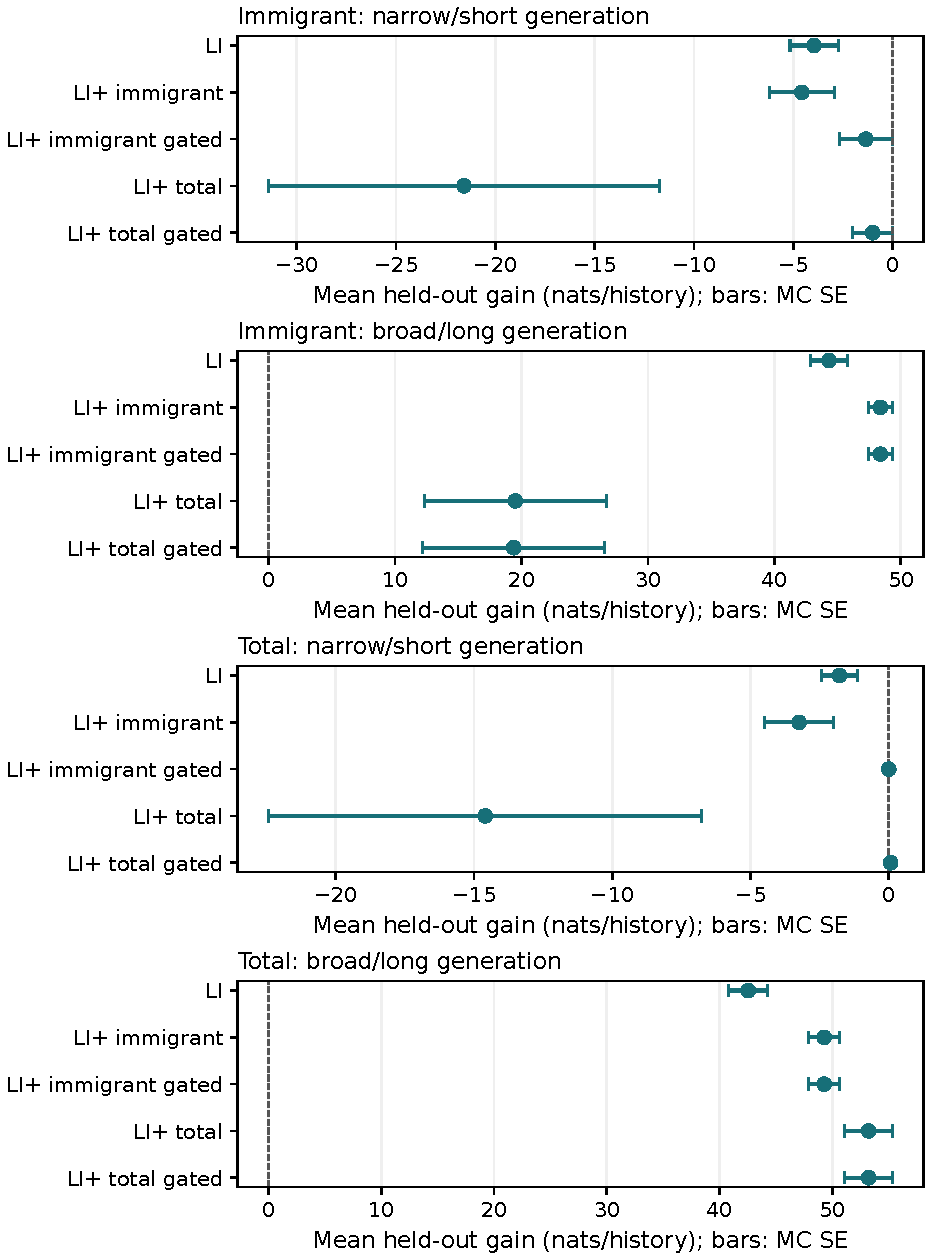
\includegraphics[width=\linewidth]{s04_expanded_mean_gains.pdf}

\caption{S04B matched-generator controls. Each panel keeps its own full linear range. Points show row means; bars show descriptive MC SE, not calibrated confidence intervals. Each procedure uses the same complete history denominator within its generating regime. The dashed zero line denotes the uninhibited floor; regimes are not pooled.}\label{fig:s04b-matched}\end{figure}


\section{Observed California fixed-backbone inhibition}

\label{sec:s04-observed-completed}

The observed comparison uses the same three California folds and 315 targets. Background and excitation nuisance inputs are fixed and shared between each candidate and its exact uninhibited floor. The common mark term cancels from each held-out joint gain, reported as floor NLL minus selected NLL.

Original LI is retained unpenalized. Magnitude-scaled LI+ is evaluated with immigrant-only and total-intensity attenuation, each with raw training selection and with the declared training-only BIC-style gate. A gate may select the exact floor. A negative held-out gain is retained, while an unresolved numerical result remains unknown rather than being assigned zero.

Table~\ref{tab:s04-observed} reports the three active empirical contrasts. Table~\ref{tab:s04-observed-boundary} partitions the twelve gate-selected or nested rows whose training solution is $\hat\eta=0$: for these cells the held-out joint contrast is identically $0.0000$ by algebraic nesting, not an independent empirical test of zero attenuation. Presenting the twelve zero rows as separate powered comparisons would overstate the evidence.

\begin{table}[htbp]\centering\caption{Active held-out joint gains (nats) relative to the shared uninhibited floor. All three rows select positive total-intensity attenuation in training and lose held-out joint score. Displayed values are empirical contrasts, not algebraic returns. Paired block intervals for raw total-intensity attenuation are reported in Section~\ref{sec:li-score-uncertainty}.}\label{tab:s04-observed}

\begin{tabular}{llllrll}\toprule Fold & Model & Gate & Status & Gain & Win & Active\\\midrule

0 & LI+ total & raw & resolved & -0.2245 & no & yes \\

1 & LI+ total & raw & resolved & -1.9529 & no & yes \\

2 & LI+ total & raw & resolved & -0.2093 & no & yes \\

\bottomrule\end{tabular}\end{table}

\begin{table}[htbp]\centering\caption{Boundary-selected rows partitioned from the active contrasts. Each displayed $0.0000$ is the exact algebraic forecast of the nested $\hat\eta=0$ floor, not an estimate of a zero physical effect. The twelve cells are three folds of four floor-selected procedures and must not be counted as twelve independent empirical test contrasts.}\label{tab:s04-observed-boundary}

\begin{tabular}{llllr}\toprule Fold & Model & Gate & Status & Algebraic gain\\\midrule

0 & LI & raw & floor-selected & 0.0000 \\

0 & LI+ immigrant & raw & floor-selected & 0.0000 \\

0 & LI+ immigrant & BIC & floor-selected & 0.0000 \\

0 & LI+ total & BIC & floor-selected & 0.0000 \\

1 & LI & raw & floor-selected & 0.0000 \\

1 & LI+ immigrant & raw & floor-selected & 0.0000 \\

1 & LI+ immigrant & BIC & floor-selected & 0.0000 \\

1 & LI+ total & BIC & floor-selected & 0.0000 \\

2 & LI & raw & floor-selected & 0.0000 \\

2 & LI+ immigrant & raw & floor-selected & 0.0000 \\

2 & LI+ immigrant & BIC & floor-selected & 0.0000 \\

2 & LI+ total & BIC & floor-selected & 0.0000 \\

\bottomrule\end{tabular}\end{table}

The BIC-style gate is a complexity penalty, not a Davies-calibrated test or a guarantee of nominal size. A training-active fit, a selected floor and a held-out win are distinct outcomes. These observed folds have been inspected retrospectively.

\begin{figure}[p]\centering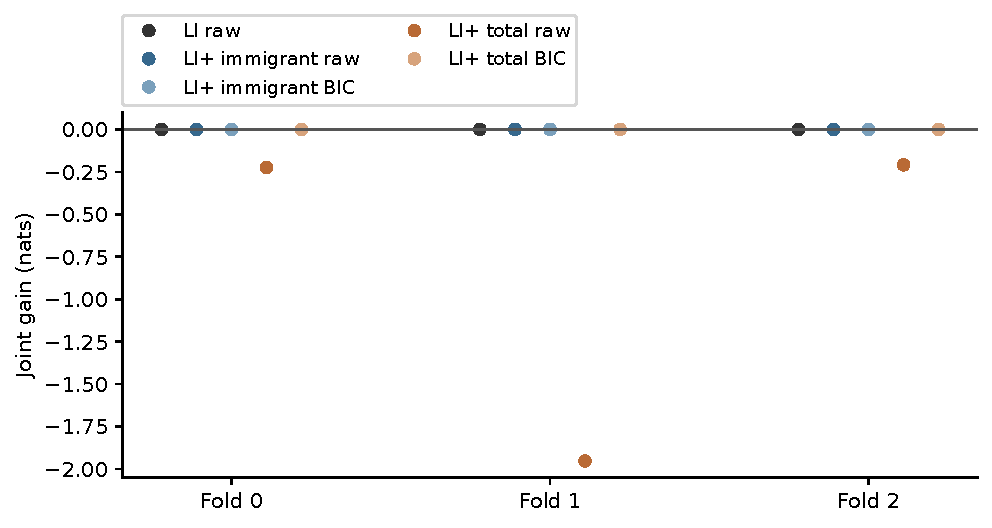
\includegraphics[width=\textwidth]{s04_observed_joint_gains.pdf}\caption{Held-out joint gains on the fixed three-fold population.}\end{figure}

\begin{center}\begin{tabular}{lrr}\toprule Fold & Training targets & Planned held-out targets\\\midrule

0 & 851 & 79 \\

1 & 930 & 167 \\

2 & 1097 & 69 \\

\bottomrule\end{tabular}\end{center}

All original LI and magnitude-scaled immigrant-only fits select their exact uninhibited floor. Raw total-intensity inhibition is active but loses held-out joint score in each fold. Its BIC-gated version selects the floor in every fold. These outcomes do not establish a predictive benefit from the revised inhibition mechanisms on this fixed observed population.


\part{Synthesis and Programme Boundaries}
\chapter{Consolidated Discussion, Limits of Inference, and Conclusion}
\label{ch:discussion}\label{ch:conclusion}\label{chap:discussion}

The programme now supports an assessment across the completed mathematical, synthetic and regional empirical arc. Its central observed-catalogue result is the failure of the tested inhibition additions to improve matched predictive scores. Large spatial gains mainly correct coarse routing and uniform cell-lift representations; these are useful diagnostic checks, but do not establish competitive forecasting superiority. Standard unweighted inverse-power ETAS beats OC in every reported California and Japan primary fold. The tested inhibition additions remain losing or tied in the observed comparisons, including after temporal refinement and localization. These statements concern declared procedures and common scored observations, not a universal ranking of all inhibitory and excitation models.
\section{What the theory separates}

The mathematical results delimit several distinct regimes. Finite positive-mode systems admit the stated first-moment stability conclusions under their link, mark and subcritical-triggering assumptions. Finite-horizon approximation does not establish an interchange of stationary and infinite-mode limits. Exact-memory counterexamples apply to specified no-feedback submodels, and the linear-response calculation concerns an auxiliary frozen-slope system. Full-law identifiability also requires assumptions stronger than those available in an observed finite catalogue. The preceding mathematical chapters state their assumptions and proofs. The new comparison in Section~\ref{sec:autonomous-nz-comparison} directly fits an autonomous finite-mode subfamily satisfying the first-moment hypotheses. Its early and late folds select positive inhibition and lose held-out score; the middle fold selects $\eta=0$ and is tied at displayed precision. This connects the stability model to an executed fitted comparison while keeping stability and predictive advantage distinct.

This separation matters for the empirical discussion. A physical model may contain loading or initial-stress memory while a finite catalogue lacks power to distinguish it from a restricted alternative. A diagnostic family may improve its training score because its likelihood geometry favours extra structure, without thereby identifying the full physical law. A small held-out loss may be numerically controlled yet limited as statistical evidence when folds overlap or were inspected. Conversely, a non-rejection is not evidence of equality. Failure to distinguish two recipes leaves a set of explanations: the data may be insufficient, the candidate may be misspecified, the optimizer may be imperfect, or the tested effect may be small over the observed horizon. The controlled studies weaken some specific explanations, but do not select a unique physical one.

At \(\eta=0\), a separately varied stress kernel disappears from the diagnostic intensity when background and triggering are held fixed. It is therefore unidentified there. The analogous physical loading argument requires finite loading and initial-stress parameters: it cannot be carried into a singular small-feedback, large-loading limit without additional analysis. Non-rejection of a shared-kernel restriction at or near zero feedback consequently does not validate equality of two physical memories.

Synthetic diagnostics further clarify, but do not erase, the inferential gap. The historical comparison with nuisance quantities supplied produced 150 detections in 150 trials, whereas a fitted setting produced 57 in 150. These are different simple-versus-composite inferential tasks; their contrast is not an intrinsic information ceiling, and it is not proof that the remainder is avoidable algorithmic inefficiency. It offers no justification for fixing the real background merely to recover apparent power. Better optimization or a larger synthetic bank can improve numerical precision without changing the scientific question.

The transformed marks add another qualification. The magnitude excess has an exponential law, while the stress and productivity transforms have finite first and infinite second moments at the declared generating parameters. That does not prevent bounded-indicator Monte Carlo summaries, but it invalidates unqualified use of Fisher-information shortcuts based on second moments. Computational stability and statistical efficiency therefore have to be defended under the declared scoring rule, not inferred from formal differentiability alone.


\section{What the temporal and mark extensions resolve}

The magnitude-history and productivity studies retain negative matched results. A class-history law can change conditional mark probabilities and, through joint fitting, timing parameters without providing additional held-out information. Its effective-scale algebra concerns the fixed observed marked history; it does not establish equality of unconditional multistep future laws. Free productivity likewise changes the fitting problem and its finite-moment regime. Its failed continuation gate is part of the result, not an omitted successful analysis waiting to be inferred.

Exposure orthogonalization separates numerical geometry from the represented family. Better Gram conditioning is useful, but an interior optimum that maps feasibly into both coordinate boxes need not give a better predictive model. The negligible score change in Stage A is therefore consistent with the algebra. Its coarse Omori bridge must be distinguished from Extension O's continuously tuned temporal law. The latter improves excitation yet leaves matched and jointly tuned inhibition losing. The national temporal loss cannot be attributed solely to having fixed the original ML triggering kernel.

Common free ML time scale improves its own temporal comparison. Parent-class time scales add an inconsistent increment and fail the registered continuation rule, leaving observed association fitting unexecuted. This does not erase the earlier completed class-history experiment: the two branches have distinct references, parameters and gates. Every claim of nonexecution in this monograph refers to its specified branch.

\section{What localization changes, and what it does not}

Regional nonclosure gives a mathematical reason to test local structure: equal pooled depletion can conceal different sums of local rates. The completed progression in Chapter~\ref{ch:nz-spatial} supplies the empirical comparison that the earlier manuscript proposed. It moves from zone-local excitation to redistribution, distance routing, projected continuous density and a factorial with stronger immigrant geography. These changes improve particular location scores, but incremental inhibition remains negative, boundary-selected or tied. A reduced whole-model penalty after localization must not be confused with a positive inhibition-minus-matched-excitation contrast.

Continuous geography retains its advantage over the cell-lift representation under the richer background. Location dominates that benefit. Temporal and background contrasts still contain losses, including changes whose pooled joint sign differs from their timing sign and whose fold signs differ from their pooled sign. Spatial normalization leaves regional intensity unchanged at fixed shared parameters; timing changes after refitting do not imply that a normalized spatial density directly creates regional events. Nor can gains from separate historical stages be concatenated as if they were one fitted comparison.

The selected spatial scales describe a bounded statistical recipe in a declared projection and domain. Endpoint selection, negative small-scale sensitivities, repeated coordinates and unknown coordinate accuracy prevent physical interaction-distance claims. Training density is an estimate of event geography under the observed record, not an identified distribution of immigrants. Missing parents, region boundaries and catalogue selection remain observation-law limitations.

\section{Transfer, competition and conditional adequacy are different questions}

California retains the primary matched temporal and location directions, and the fitted target beats its no-trigger reference. EP nevertheless wins the joint comparison in every original primary window, chiefly through conditional location. The higher-magnitude sensitivity and annual/sequence accounting retain their separate denominators and do not convert retrospective inspection into untouched confirmation. The Ridgecrest active partition is a predetermined-in-form retrospective time union; it is not a causal assignment of individual aftershocks. These regional score conclusions use recovered original fit and score records with checked hashes and source identities, rather than newly recomputed regional scores; the original audit scopes remain distinct from this recovery.

Japan transfers the continuous-versus-lifted location direction but reverses the Omori-versus-fixed-ML timing direction in every scored window. The combined descriptive transfer rule therefore fails. EP again wins jointly. A statement that ``the improvement transfers'' without naming the component and reference would obscure a central negative finding. The explicit complete-primary selection rule also limits the population to which the JMA comparison applies; excluded unresolved records are not silently imputed.

The frozen OC conditional simulations ask another question. Material count, gap, spatial and subblock discrepancies survive the complete identity/count/mark/exposure audit. Tied diagnostic values require insertion intervals, particularly for empty cells; a single randomized rank would hide that ambiguity. The full raw replay has narrower path coverage than the aggregate audit. These diagnostics show material conditional inadequacy of OC across the three origins. Deterministic immigrant exposure is an accounting coordinate, not a random calibration test, and total/trigger exposure ranks are redundant. EP's log-score victory stands on its own; Section~\ref{sec:s05-completed} shows fixed-state discrepancies for EP too \citep{Schorlemmer2007,Zechar2010}.

The completed matched magnitude-history study (Section~\ref{sec:s02-completed}) separates frequent small positive fitted gains from evidence calibrated against its empirical null bank. Matching productivity reduces the mean GLR relative to the misspecified candidate, but positive selection remains common. Exceedances of the same-bank empirical threshold do not establish independent Type I error control or a physical explanation.

The four-arm spatial comparison (Section~\ref{sec:s03-completed}) addresses a different contrast from the earlier coarse cell-lift checks. EP retains a regional joint advantage over OC in California and New Zealand, chiefly through location. Fold contrasts vary; the comparison neither establishes universal EP superiority nor causally decomposes tail shape and background effects.

The expanded California backtest (Section~\ref{sec:s06-completed}) has a distinct retrospective episode roster and variable procedure contrasts: EP does not win every episode. Its causal training prefixes do not make the inspected roster prospective or independent. In Japan, fixing the background trend at zero reduces the pooled OC--FC timing deficit but leaves every fold negative. The trend ablation therefore does not remove the reversal or rescue the combined descriptive transfer rule.

\section{Continuous local inhibition and the zero-strength boundary}

The LI extension attenuates only the immigrant contribution without spatial renormalization. The field uses unit stress marks and all eligible strictly earlier recorded parents. Every eligible event therefore contributes the same inhibition amplitude regardless of magnitude, while triggering is unattenuated. This is a restrictive diagnostic of immigrant attenuation, not a physical stress-shadow model or whole-intensity suppression. At zero strength it nests OC exactly, while range and memory disappear from the law.

All selected observed California LI states lie at that boundary. The tiny retained positive floating-point difference from OC is a numerical tie, not a predictive gain. The separately archived OC--EP and LI--EP values retain distinct source identities even though their displayed rounded values agree. Range and memory display conventions at zero do not identify physical scales. EP's better score remains a competitive result rather than a calibration certificate.

Every fixed-seed regime matters. In the historical initial eight-dataset study, all four null controls lose held-out score, including a loss of 148.65 nats. This shows that nesting the null in training does not protect future performance: estimation variability and overfitting remain plausible. Held-out losses alone do not establish an optimization defect or estimate a false-positive rate. Losses under narrow/short positive inhibition prevent an assertion that the procedure reliably detects inhibition whenever it exists. Broad/long positive examples demonstrate success under those retained laws, with small test counts. The regimes have different laws and denominators; an aggregate success percentage would not estimate a meaningful common power. No inconvenient seed, cap or recovery history is replaced by a more favourable outcome.

The expanded matrix in Section~\ref{sec:s04-expanded} separates original LI, magnitude-scaled immigrant attenuation and total-intensity attenuation. Under the original unit-mark, immigrant-only generating law, magnitude-scaled immigrant-only inhibition has a positive mean gain in the broad/long regime, whereas total-intensity attenuation has a negative mean there. Both LI+ procedures are alternatives to that generating law, so this comparison does not measure their power under matched LI+ generation. The matrix reports Monte Carlo uncertainty by regime, and shows that gating can remove null overfitting while also selecting no inhibition in the narrow/short positive regime. This extends procedural sensitivity evidence without establishing physical absence or nominal test size.

The separate matched-generator extension in Section~\ref{sec:s04b-matched} generates magnitude-scaled immigrant-only and total-intensity histories. The generator counters change the interpretation of its narrow/short immigrant setting: 19 of 20 histories have no rejected proposals. This is a weakly realized control, not evidence of reliable recovery or its general impossibility. The total-attenuation setting rejects offspring and is a different experiment. Both matched raw procedures retain negative narrow/short mean gains against either floor. The original broad/long wins all use a fixed nuisance backbone. In the executed intercept sensitivity (Section~\ref{sec:s04b-refitted}), fitting the uninhibited background on training leaves matched mean gains of 5.1631 and 9.7367 nats, with 19/20 and 18/20 wins. This removes most of the large fixed-floor advantage but not all of it. The saved inhibitory parameters, gates and remaining nuisance coordinates are unchanged, so the comparison does not establish the performance of jointly refitted families. The fitted-parameter table also shows boundary concentration; an off-floor fit need not recover the generating parameters.

The completed magnitude-scaled observed comparison (Section~\ref{sec:s04-observed-completed}) retains the same conclusion: immigrant-only LI+ selects no inhibition in every fold. Raw total-intensity attenuation selects positive inhibition but loses held-out joint score in every fold; its complexity-gated version returns to the exact uninhibited floor. This fixed-backbone comparison addresses the revised diagnostic procedures, not a general test of physical stress shadows.

The completed conditional comparison (Section~\ref{sec:s05-completed}) retains discrepancies for both OC and EP under the two continuous-statistic omnibus procedures at each origin. The retained minimum-rank procedure does not reject at the declared level. Better comparative log score and conditional adequacy are therefore distinct: EP wins important score comparisons without thereby passing these diagnostic checks. Fitted states are held fixed, and no joint cross-origin null or parameter-uncertainty integration is claimed.

\section{Interpretation of the completed comparisons}

The New Zealand programme adaptively reused the same 612 test events: earlier test scores informed later model design and parameter bounds. Freezing each stage did not erase this dependence \citep{Dwork2015}. The inspected historical windows, overlapping training prefixes and dependent earthquake histories preclude event-iid confidence intervals and untouched-confirmation language. The singular zero-strength boundary does not come with a justified Wilks or half-chi-squared reference law. A bounded multistart search, independent score reconstruction and near-optimal forecast-spread check are useful controls, but are not global-optimization proofs.


The literature classifications in Appendix~\ref{app:literature_status} identify inherited triggering kernels, established stability machinery and restricted model-specific derivations. The contribution is the stated analysis and the executed procedure comparisons.

\section{Conclusion}

Mathematical legitimacy, identification, estimation, competitive prediction and calibration are distinct achievements. The finite-mode and finite-history results provide a restricted foundation; fitted nuisance parameters, stronger benchmarks, calibration and transfer constrain its empirical reach. The tested inhibition additions do not establish predictive success on the observed catalogues. This does not imply physical absence. Positive ablations, negative contrasts, boundary selections and completed failed gates remain part of that assessment.

\appendix
\chapter{Archival Source Map, Notation, Score Semantics, and Literature Classification}\label{app:source-map}
\label{app:evidence}

\section{What the manuscript and its companion files reproduce}

The internal project and addendum records are retained in \path{paper/supplements/project_source_records.bib}, as source-availability metadata rather than peer-reviewed bibliography entries. The exact consulted external preprint and its later journal publication remain distinct because the text cites version-specific equations.

The companion source builds this unified manuscript from retained LaTeX, native conversions and saved figures. The original compact-release availability statements below describe the historical baseline; the present delivery additionally embeds the sources, figures, claim ledger and authority copies needed for its editorial rebuild and reconciliation. The document build itself does not rerun historical scientific studies. Rebuilding a plot from a retained table is different from regenerating its histories, refitting its models and recalibrating its test. Each derived data file and figure records its source in the figure manifest. Illustrative mathematical figures are labelled as such; they are not synthetic catalogue outcomes.

The earlier 40-page manuscript is not redistributed in this public repository. The reconstructed New Zealand, California and Japan catalogue records are now supplied under \path{reproduction/}, together with the raw provider inputs, explicit selection rules and portable cohort-reconstruction commands. The catalogue providers, access locations, original snapshot hashes and terms are documented in \path{docs/data.md}. Reacquiring a live catalogue does not guarantee recovery of the historical snapshot. The earlier manuscript's frozen catalogue, original fitting code, complete optimization records and editable source remain unavailable.

The principal data snapshot was retrieved on 15 October 2026 from GeoNet's WFS interface. Its bundled selected CSV is \path{reproduction/nzca/expected/geonet_M5_shallow_1960_2026.csv}, with SHA256
\begin{quote}\small\ttfamily
feacccb7581d1c4c33f88874cd6b198c41639da6930a7fc35e46f910a594fb3e.
\end{quote}
The saved metadata defines the exact geographic, depth, magnitude, event-type and clock rules. The 1960-origin observation window is 24,394 days, with 15 October 2026 excluded. The archived FDSN selection contains 914 events: all 913 primary IDs and one additional ID. These are two interfaces/snapshots from one provider, not independent physical catalogues.

\section{Canonical authorities for the main results}

Table~\ref{tab:authority_map} gives the archive-relative entry points needed to inspect the main claims. Narrative summaries point to their underlying machine-readable outputs. A source report establishes what was reported and retained; a hash establishes byte consistency. Neither alone certifies a physical mechanism or every historical execution.

The \href{https://github.com/Drefetr/InhibitoryEarthquakeModels/blob/3e76a174cf4f58ce601c6c9640c4d0c11168813f/paper/supplements/source_availability.json}{public availability register} records the historical compact-release subset and references to the research archive. The historical source index is retained as metadata in \href{https://github.com/Drefetr/InhibitoryEarthquakeModels/blob/3e76a174cf4f58ce601c6c9640c4d0c11168813f/provenance/historical_v4_source_index.json}{historical source index}; its old included paths describe release v4, not this repository. Current recovered inputs and executable replays are indexed separately in \path{reproduction/README.md}; current payload membership is recorded in \path{MANIFEST.json}. The earlier manuscript PDF remains outside this distribution.

\begin{longtable}{@{}>{\raggedright\arraybackslash}p{0.20\textwidth}>{\raggedright\arraybackslash}p{\dimexpr\textwidth-0.20\textwidth-2\tabcolsep\relax}@{}}
\caption{Canonical source map. Display names identify archive-relative authorities; stable IDs map to the full paths in the source index. This is not a promise that every historical payload is embedded in a compact manuscript release.}\label{tab:authority_map}\\
\toprule
Topic & Authority and scope \\
\midrule
\endfirsthead
\toprule Topic & Authority and scope \\\midrule
\endhead
Finite-mode analysis & \nolinkurl{A_finite_mode_audit.md}; accompanying \texttt{S21}: \nolinkurl{A_theorems.tex}. State assumptions, construction, coupling and approximation scope. \\
% Exact archive paths: iteration_4/reports/A_finite_mode_audit.md; iteration_4/manuscript_revisions/A_theorems.tex
Exact memory and response & \nolinkurl{B_memory_response.md}; \texttt{S22}: \nolinkurl{B_propositions.tex}. No-feedback obstructions and the auxiliary response are separate results. \\
% Exact archive paths: iteration_4/reports/B_memory_response.md; iteration_4/manuscript_revisions/B_propositions.tex
Identification and score bounds & \texttt{S23}: \nolinkurl{C_identifiability.md}; \texttt{S03}: \nolinkurl{restricted_score_bound.md}; \texttt{S06}: \nolinkurl{power_response_corollary.md}. Positive-feedback and fixed-rule assumptions apply locally to each proposition. \\
% Exact archive paths: iteration_4/reports/C_identifiability.md; iteration_13/reports/restricted_score_bound.md; iteration_15/reports/power_response_corollary.md
Amplitude profiling & \texttt{S12}: \nolinkurl{A_amplitude_proposition.md}; \texttt{S13}: \nolinkurl{background_balance_corollary.md}. Conditional negative-log-likelihood calculus, not a global optimizer theorem. \\
% Exact archive paths: iteration_23/reports/A_amplitude_proposition.md; iteration_23/reports/background_balance_corollary.md
Reconstructed catalogue & \texttt{S24}: \nolinkurl{catalogue_metadata.json}; \texttt{S25}: \nolinkurl{research_report.md}. Archived new snapshot, selection and independent reconstruction. \\
% Exact archive paths: iteration_5/data/processed/catalogue_metadata.json; iteration_5/reports/research_report.md
Known-law comparison & \texttt{S09}: \nolinkurl{completed_evaluation.md}; \nolinkurl{completed_results.json}. All 2,149 scores accepted, including five validated imports; no new histories for this comparison. \\
% Exact archive paths: iteration_19/reports/completed_evaluation.md; iteration_19/reports/completed_results.json
Background comparison & \texttt{S11}: \nolinkurl{research_report.md}; \nolinkurl{completion_summary.json}. Accepted completion of the supplied-background and estimated-background procedures. \\
% Exact archive paths: iteration_22/reports/research_report.md; iteration_22/results/completion_summary.json
Optimizer robustness & \texttt{S14}: \nolinkurl{research_report.md}. Ten selected difficult histories; the earlier preparation and failed strict branches are not substituted for completion. \\
% Exact archive paths: iteration_24/completion/reports/research_report.md
Raw ablation & \texttt{S15}: \nolinkurl{research_report.md}. Ten-history level/trend raw-statistic comparison, not calibrated power. \\
% Exact archive paths: iteration_25/completion/reports/research_report.md
Level-only calibration & \texttt{S16}: \nolinkurl{research_report.md}; \texttt{M09}: \nolinkurl{summary.json}. All 2,149 fresh fits and accepted matched-null decisions. \\
% Exact archive paths: iteration_26/completion/reports/research_report.md; iteration_26/completion/results/summary.json
Observed prediction & \texttt{S19}: \nolinkurl{research_report.md}; \texttt{M18}: \nolinkurl{summary.json}. Three folds, five declared families, 612 scored test events. \\
% Exact archive paths: iteration_27/reports/research_report.md; iteration_27/results/observed_analysis/summary.json
Heterogeneity and source sensitivity & \texttt{S20}: \nolinkurl{research_report.md}; \nolinkurl{summary.json}; \nolinkurl{A_source_comparison.json}. Fixed-parameter temporal decomposition and matched source-value sensitivity. \\
% Exact archive paths: iteration_28/reports/research_report.md; iteration_28/results/publication/summary.json; iteration_28/results/A_source_comparison.json
\bottomrule
\end{longtable}


\section{Stable source supplement identifiers}\label{sec:source-supplements}
The identifiers below retain the identity of historical documentary sources. Their exact original files are supplied in \path{reproduction/historical_fits/historical_fit_package.zip}; \path{reproduction/historical_fits/source_availability.json} maps each identifier to its archive member and hash. These documentary source identifiers are distinct from the later follow-up study identifiers. The mathematical arguments are given in Chapters~\ref{ch:models}--\ref{ch:inference}. The public repository also retains \path{paper/supplements/explanatory_supplement.pdf}. Archive recovery supplies existing evidence and does not constitute a new scientific execution.

\begin{longtable}{@{}>{\raggedright\arraybackslash}p{0.09\textwidth}>{\raggedright\arraybackslash}p{\dimexpr\textwidth-0.09\textwidth-2\tabcolsep\relax}@{}}
\caption{Stable documentary source keys, display filenames and public status. Full original archive-relative paths are retained in the source index for provenance.}\label{tab:source-keys}\\
\toprule Key & Archived document \\ \midrule\endfirsthead
\toprule Key & Archived document \\ \midrule\endhead
\hypertarget{S01}{}\label{source:S01}\texttt{S01} & \nolinkurl{summary.json}. \textit{Recovered original} \\
% Exact archive paths: iteration_12/results/aggregate/2026-10-16T061247128773_0000/summary.json
\hypertarget{S02}{}\label{source:S02}\texttt{S02} & \nolinkurl{reference_score_geometry.md}. \textit{Recovered original} \\
% Exact archive paths: iteration_13/reports/reference_score_geometry.md
\hypertarget{S03}{}\label{source:S03}\texttt{S03} & \nolinkurl{restricted_score_bound.md}. \textit{Recovered original} \\
% Exact archive paths: iteration_13/reports/restricted_score_bound.md
\hypertarget{S04}{}\label{source:S04}\texttt{S04} & \nolinkurl{stable_process_irregular_score.md}. \textit{Recovered original} \\
% Exact archive paths: iteration_13/reports/stable_process_irregular_score.md
\hypertarget{S05}{}\label{source:S05}\texttt{S05} & \nolinkurl{positive_eta_response.md}. \textit{Recovered original} \\
% Exact archive paths: iteration_15/reports/positive_eta_response.md
\hypertarget{S06}{}\label{source:S06}\texttt{S06} & \nolinkurl{power_response_corollary.md}. \textit{Recovered original} \\
% Exact archive paths: iteration_15/reports/power_response_corollary.md
\hypertarget{S07}{}\label{source:S07}\texttt{S07} & \nolinkurl{power_engine.py}. \textit{Recovered original} \\
% Exact archive paths: iteration_16/code/power_engine.py
\hypertarget{S08}{}\label{source:S08}\texttt{S08} & \nolinkurl{research_report.md}. \textit{Recovered original} \\
% Exact archive paths: iteration_16/reports/research_report.md
\hypertarget{S09}{}\label{source:S09}\texttt{S09} & \nolinkurl{completed_evaluation.md}. \textit{Recovered original} \\
% Exact archive paths: iteration_19/reports/completed_evaluation.md
\hypertarget{S10}{}\label{source:S10}\texttt{S10} & \nolinkurl{restricted_history.py}. \textit{Included} \\
% Exact archive paths: iteration_20/code/restricted_history.py
\hypertarget{S11}{}\label{source:S11}\texttt{S11} & \nolinkurl{research_report.md}. \textit{Recovered original} \\
% Exact archive paths: iteration_22/reports/research_report.md
\hypertarget{S12}{}\label{source:S12}\texttt{S12} & \nolinkurl{A_amplitude_proposition.md}. \textit{Recovered original} \\
% Exact archive paths: iteration_23/reports/A_amplitude_proposition.md
\hypertarget{S13}{}\label{source:S13}\texttt{S13} & \nolinkurl{background_balance_corollary.md}. \textit{Recovered original} \\
% Exact archive paths: iteration_23/reports/background_balance_corollary.md
\hypertarget{S14}{}\label{source:S14}\texttt{S14} & \nolinkurl{research_report.md}. \textit{Recovered original} \\
% Exact archive paths: iteration_24/completion/reports/research_report.md
\hypertarget{S15}{}\label{source:S15}\texttt{S15} & \nolinkurl{research_report.md}. \textit{Recovered original} \\
% Exact archive paths: iteration_25/completion/reports/research_report.md
\hypertarget{S16}{}\label{source:S16}\texttt{S16} & \nolinkurl{research_report.md}. \textit{Recovered original} \\
% Exact archive paths: iteration_26/completion/reports/research_report.md
\hypertarget{S17}{}\label{source:S17}\texttt{S17} & \nolinkurl{adequacy.py}. \textit{Included} \\
% Exact archive paths: iteration_27/code/adequacy.py
\hypertarget{S18}{}\label{source:S18}\texttt{S18} & \nolinkurl{observed_frozen.json}. \textit{Recovered original} \\
% Exact archive paths: iteration_27/configs/observed_frozen.json
\hypertarget{S19}{}\label{source:S19}\texttt{S19} & \nolinkurl{research_report.md}. \textit{Recovered original} \\
% Exact archive paths: iteration_27/reports/research_report.md
\hypertarget{S20}{}\label{source:S20}\texttt{S20} & \nolinkurl{research_report.md}. \textit{Recovered original} \\
% Exact archive paths: iteration_28/reports/research_report.md
\hypertarget{S21}{}\label{source:S21}\texttt{S21} & \nolinkurl{A_theorems.tex}. \textit{Recovered original} \\
% Exact archive paths: iteration_4/manuscript_revisions/A_theorems.tex
\hypertarget{S22}{}\label{source:S22}\texttt{S22} & \nolinkurl{B_propositions.tex}. \textit{Recovered original} \\
% Exact archive paths: iteration_4/manuscript_revisions/B_propositions.tex
\hypertarget{S23}{}\label{source:S23}\texttt{S23} & \nolinkurl{C_identifiability.md}. \textit{Recovered original} \\
% Exact archive paths: iteration_4/reports/C_identifiability.md
\hypertarget{S24}{}\label{source:S24}\texttt{S24} & \nolinkurl{catalogue_metadata.json}. \textit{Recovered original} \\
% Exact archive paths: iteration_5/data/processed/catalogue_metadata.json
\hypertarget{S25}{}\label{source:S25}\texttt{S25} & \nolinkurl{research_report.md}. \textit{Recovered original} \\
% Exact archive paths: iteration_5/reports/research_report.md
\hypertarget{S26}{}\label{source:S26}\texttt{S26} & \nolinkurl{SUPERVISOR_REVIEW_ADDENDUM.txt}. \textit{Recovered original} \\
% Exact archive paths: review_handoff/2026-10-18/deepseek_cli_review_20261018-115244/SUPERVISOR_REVIEW_ADDENDUM.txt
\hypertarget{S27}{}\label{source:S27}\texttt{S27} & \nolinkurl{research_handoff.md}. \textit{Recovered original} \\
% Exact archive paths: review_handoff/2026-10-18/output/research_handoff.md
\bottomrule
\end{longtable}


\section{Unified study-to-chapter map}

The pinned library contains the baseline, Addenda I--V and the following completed follow-up strands. Their authoritative JSON remains in the named upstream runs; the ledger records exact files, fields and SHA-256 identities. The withdrawn F addendum is retained in the historical source archive; Addendum II in Chapter~\ref{ch:temporal-extensions}; Addendum III in Chapter~\ref{ch:nz-spatial}; Addendum IV in Chapters~\ref{ch:external}--\ref{ch:calibration}; and Addendum V in Chapter~\ref{ch:local-inhibition}. The section-level crosswalk accompanies this edition.

\begin{longtable}{@{}p{.78\textwidth}p{.16\textwidth}@{}}
\caption{Complete follow-up roster and integrated destination. Dates are run identifiers, not independent evidence counts.}\\
\toprule Pinned strand & Chapter \\\midrule\endfirsthead
\toprule Pinned strand & Chapter \\\midrule\endhead
\nolinkurl{california_schema_repair_20261025T044000Z} & 11 \\
\nolinkurl{competitive_benchmarks_20261025T065609Z} & 11 \\
\nolinkurl{conditional_calibration_20261025T085151Z} & 12 \\
\nolinkurl{kernel_and_continuous_space_20261024T183658Z} & 9 and 10 \\
\nolinkurl{local_inhibition_gpu_resume_20261028T172954Z} & 13 \\
\nolinkurl{magnitude_history_20261023T205716Z} & 9 \\
\nolinkurl{magnitude_prediction_20261023T222049Z} & 9 \\
\nolinkurl{multitype_temporal_decay_20261024T173017Z} & 9 \\
\nolinkurl{orthogonal_stress_and_kernel_20261024T082952Z} & 9 \\
\nolinkurl{productivity_slope_20261024T023501Z} & 9 \\
\nolinkurl{score_robustness_20261025T102500Z} & 11 \\
\nolinkurl{sequence_score_audit_20261025T193331Z} & 11 \\
\nolinkurl{spatial_continuation_20261024T102859Z} & 10 \\
\nolinkurl{spatial_local_inhibition_20261024T094130Z} & 10 \\
\nolinkurl{temporal_spatial_background_20261024T211225Z} & 10 \\
\nolinkurl{third_region_transfer_20261026T001254Z} & 11 \\
\bottomrule\end{longtable}

\section{Score-field custody}

Section~\ref{sec:master-scores} defines the canonical $P,Q,E,C=-E,M$ notation. Historical temporal and LI raw \texttt{E} fields denote event-logsum differences; sequence \texttt{timing\_compensator} denotes a signed difference in nonnegative exposure. The pinned field dictionary is preserved with its source identity. No archived key is renamed in the authority copy, and no sign is inferred from a key name alone. The source ledger distinguishes raw values, derived differences and displayed rounding.
\section{Historical theoretical notation and scope}
\label{app:notation}

\begin{longtable}{@{}p{0.17\textwidth}p{0.78\textwidth}@{}}
\caption{Core notation. Individual propositions specify any additional conditions and distinguish the physical and diagnostic uses.}\\
\toprule Symbol & Meaning \\
\midrule\endfirsthead
\toprule Symbol & Meaning \\\midrule\endhead
$T_i,M_i$ & Event time and fresh magnitude/mark; predictable intensity at $T_i$ uses strictly earlier events. \\
$\Phi_s,h_e$ & Stress relaxation and triggering density. A shared restriction may relate them, but they are varied separately when testing identification. \\
$X$ & Latent physical stress, including specified loading, initial state and event depletion. \\
$B(t)$ & Independently specified diagnostic background; it may be nonstationary and is not the physical loading closure. \\
$G_s(t),H_e(t)$ & Marked diagnostic depletion and normalized triggering features based on past history. \\
$\eta$ & Nonnegative diagnostic inhibition coefficient; it is not automatically the original physical stress parameter. \\
$n$ & Physical mean productivity $n=\E _F\kappa(M)<1$; in the diagnostic convention $\E _F\kappa(Q)=1$ and $n$ is the coefficient outside $H_e$. \\
$\ell,F$ & In Chapter~\ref{ch:inference}, log-likelihood and its negative; $F$ elsewhere denotes the mark law and $\ell$ the auxiliary response slope. Local definitions fix these uses. \\
$A=e^a,p_i$ & Background amplitude and fitted background mixture weight at event $i$. The weights are not identified causal parent labels. \\
$a_{\mathrm{rel}},\beta_{\mathrm{rel}}$ & Auxiliary-response coefficient $(1-n)\tau^{-\alpha}$ and exponent $1-\alpha$; $a$ remains the background intercept. \\
$\gamma$ & Feedback gain $m_1\ell$ in the auxiliary response; the stress-mark exponent is separately defined in the generating law. \\
$\alpha$ & Fractional relaxation index where used, with its permitted range stated in the relevant model. \\
$\beta$ & Excess-mark rate in the exponential mark model; the Lyapunov weight in Theorem~\ref{thm:finite_mode} is a separate local use. A plug-in mark-rate estimate is not automatically a joint marked-intensity MLE. \\
\bottomrule
\end{longtable}

\section{Focused literature comparisons}
\label{app:literature_status}

The contribution classifications distinguish inherited components, applications of established theory and model-specific derivations. Each mathematical result is stated and proved under its own hypotheses in the main chapters.

\begin{longtable}{@{}>{\raggedright\arraybackslash}p{0.23\textwidth}>{\raggedright\arraybackslash}p{\dimexpr\textwidth-0.23\textwidth-2\tabcolsep\relax}@{}}
\caption{Contribution classifications and primary-source context.}\label{tab:contribution-classification}\\
\toprule Result & Classification and source comparison \\ \midrule\endfirsthead
\toprule Result & Classification and source comparison \\ \midrule\endhead
Mittag--Leffler triggering & \textbf{Inherited component / application}. \citet{DavisBaeumerWang2024}, equations (11)--(12), give the derivative-related triggering kernel and marked productivity. \\
Shared depletion and triggering & \textbf{Model specialization; no priority claim}. \citet{PetrilloZhuangLippiello2023}, equations (10)--(11), uses an additive permanent correction; the present restriction multiplies a positive background by relaxing depletion and sets \(h=-\Phi'\). An equation difference does not establish firstness. \\
Theorem~\ref{thm:finite_mode} & \textbf{Application of weak Harris theory}. The model-specific construction, drift and coupling verify the hypotheses of \citet{HairerMattinglyScheutzow2011}, Theorem 4.8 and Corollary 4.11. \\
Proposition~\ref{prop:heavy-moments} & \textbf{Self-contained moment derivation}. A recent-jump truncation argument identifies the divergent second moments while retaining first-moment stability; no priority claim. \\
Propositions~\ref{prop:quantitative-kernel}--\ref{prop:qualitative-kernel} & \textbf{Coupling derivations / scope correction}. Quantitative half-line control and qualitative local truncation are distinct. The correction does not establish an invariant infinite-mode limit. \\
Proposition~\ref{prop:exact-obstruction} & \textbf{Compensated shot-noise specialization}. The displayed characteristic-function and moment arguments apply to the stated no-feedback submodel; no general nonlinear or novelty claim. \\
Proposition~\ref{prop:auxiliary-response} & \textbf{Self-contained linear specialization}. The explicit resolvent uses established Stieltjes/complete-Bernstein relaxation tools; see \citet{MeerschaertToaldo2019}, Section 2.1. Its nonlinear interpretation remains restricted. \\
Zero-feedback nonidentification & \textbf{Direct observation-law consequence}. At fixed finite loading and initial stress, stress memory vanishes from the diagnostic law at zero feedback. The singular divergent-loading closure is separate. \\
Positive-feedback identification & \textbf{Restricted nonlinear derivation; no priority claim}. The known-transform, empty-history, unbounded-mark experiment differs from the linear representation setting of \citet{DavisKresinBaeumerWang2026}, Theorem 3. It does not establish finite-catalogue estimation. \\
Visibility and score bounds & \textbf{Self-contained finite-horizon derivations}. Matched nonnegative histories and the stated weighted moment conditions are essential. No general information, boundary asymptotics or universal detection threshold follows. \\
Remark~\ref{prop:regional_nonclosure} & \textbf{Conditional pooling algebra}. Equal total depletion need not give equal summed local rates. No empirical attribution to pooling follows. \\
Conditional amplitude profile & \textbf{Finite-history calculus / convexity application}. The conditional profile, its balance and curvature do not establish a global optimum over trend and inhibition. \\
Fixed-rule positive-inhibition response & \textbf{Likelihood differentiation derivation}. The fixed complete-data rule and positive-inhibition envelope differ from the fitted diagnostic setting in \citet{KlingVetter2024}. No monotonicity or boundary calibration is claimed. \\
\bottomrule
\end{longtable}


\chapter{Master Numerical Custody, Audit Rosters, and Parameter Ledger}\label{app:custody}

\section{Machine-readable custody and rebuild}

The delivery's \path{validation/MASTER_CLAIM_LEDGER.json} binds empirical numbers and table entries to the retained authorities. Each entry identifies a file hash, a JSON pointer or explicit documentary locator, the displayed value and its derivation, with comparator, component and denominator where applicable. \path{validation/numeric_reconciliation_receipt.json} reports actual comparisons and unresolved limitations. Hash agreement establishes identity; it is not a theorem or a reconstruction of the generating computation.

The historical source maps below remain useful for original calculations that were not distributed in the compact public release. The unified source is self-contained for LaTeX compilation. The separate recovered-input bundle distributes earthquake records under provider terms and supplies executable cohort and numerical-replay entry points; it does not recover the original missing manuscript. The document build invokes Tectonic at the pinned version and the production validator checks references, citations, figures, log warnings and page edges, then renders every page for inspection. It imports no scientific fitting or simulation entry point.

\section{Parameter and procedure custody}

The original origin-specific predictive parameters are retained in Chapter~\ref{ch:observed} and in \path{paper/supplements/predictive_parameters.json}. The design chapter records the finite spectral recipe and historical generator. Addendum II's reconciled parameter/procedure tables and the A/B/O summaries bind the temporal extensions; the spatial summaries bind routing, density and factorial choices. The external/LI protocol subset supplies nuisance freezing, bounds, starts, fallback rules, exact floors and tie selection. Chapter~\ref{ch:local-inhibition} retains the full LI start schedule and all controls. A training-selected parameter, a numerical floor and a boundary display convention are recorded separately.

The main numerical rosters must remain local to their studies. Counts of procedures, prescribed starts, solver returns, retained candidates, exact floors and audited scores are not interchangeable. Raw-history score reconstruction is also distinct from checking exported aggregate arithmetic. The III--V audit answers those distinctions explicitly; a full aggregate calibration audit does not mean every simulated diagnostic was independently replayed from raw paths.
\section{Completed evidence}

The initial calibration retained 1,999 cases for each of two restrictions, or 3,998 rows, under its declared recovery policy. The later paired study completed 150 fresh pairs, or 300 full-fit cases. The known-law and background comparisons reused specified saved histories and retained their reference/query identities. Fresh fitting of a saved history is not a fresh independent catalogue replication. The smaller planning cohorts were not pooled with the later cohort to improve its reported precision.

The observed five-family comparison completed all 477 planned records, 411 mandatory optimization start lineages and 30 selected numerical controls.

The final fixed-parameter audit completed 90 evaluations, 45 quadrature-order pairs, 18 temporal additivity controls and 913 source matches. That fixed-parameter audit did not introduce a spatial model, new fitting, new simulation or another catalogue download. Later spatial and external studies are separately integrated in Part III. Spatial and mark group tables partition event terms; their absence of a local compensator is a limit of the object computed, not a missing integral that can be supplied by arbitrarily allocating the national exposure.

\section{Numerical control is not a statistical or physical certificate}

The likelihood uses predictable pre-event features, the full observation window and its quiet intervals. Numerical controls compare the declared finite-mixture/clock representation and quadrature refinements at selected points. An empirical envelope or agreement at two orders is not a proven integration-error bound. Histories with extreme marks or closely spaced clocks remain in the procedure through declared numerical policies; unresolved outcomes cannot be silently converted into non-rejections.

Likewise, a solver's small gradient, successful exit or repeated winner is not a global optimality theorem. The ten-history robustness study materially reduces the appeal of merely increasing optimizer limits on that selected set, without validating all historical fits. The mathematical convexity of the conditional amplitude objective is narrower than joint convexity of the remaining profile. The manuscript retains these distinctions when interpreting the numerical evidence.

\section{Computational and AI assistance}\label{sec:ai-assistance}
The completed summaries were accepted within the research archive's internal review. This manuscript does not present model-assisted agreement as independent academic refereeing. Human collaborators are Drefetr and magna-nz, identified by their reported GitHub handles. AI systems used as tools, as reported in the project history, include Claude Opus 5.5, DeepSeek 4.1 Flash, Gemini 4.0 Argon, GPT 6.0 Astra and GPT 6.1 Sol; these systems are not listed as authors. The bulk of the project work was performed by AI agents: Claude Opus 5.5 and GPT 6.0 Astra developed the initial outline and specification; GPT 6.1 Sol coordinated an agent swarm comprising GPT 6.1 Sol and DeepSeek 4.1 Flash subagents; GPT 6.0 Astra and Gemini 4.0 Argon provided review. These roles describe the development history reported by the collaborators, rather than independently verified model identities for every historical call. The release-v4 finalisation used native Codex agents without external DeepSeek calls. Reviewing retained sources and arithmetic is distinct from rerunning the historical studies.



\section{Reading the detailed audit records}
The following records supply the complete per-window, parameter, protocol and diagnostic tables supporting Chapters~\ref{ch:temporal-extensions}, \ref{ch:nz-spatial} and \ref{ch:calibration}. Their original comparison signs, denominators, failed gates and numerical representations are retained. Each chapter links to the relevant record; the main text retains its primary comparisons and interpretation.
\section{Temporal and mark-extension audit tables}\label{app:audit09}

\subsection{Implementation and validation}
\label{app:audit09-pilot-implementation}


The new numerical core is standalone C++17 with a base-R interface. The preserved Python estimator uses its original CUDA/FP64 primary route and declared failure-only recovery. Core special-function support is explicitly limited to temporal shape 0.5 or 1; unsupported shapes fail. No general contour implementation was silently substituted.

Validation evidence includes:

\begin{itemize}
\item Original released ml.m executed under GNU Octave 11.3.0 after one private copyright-preserving dispatch-byte change; all 78 checked shape/scale/time cases passed. Maximum absolute survival/ML discrepancy was $\text{\texttt{2.33e-15}}$. This is a kernel reference bridge, not a full author-fit reproduction.
\item Independent SciPy special-function/spectral-quadrature and high-precision Decimal checks on 84 kernel cases plus the saved clock fixtures. These mathematical audits used Python; R was tested separately as an end-to-end interface.
\item Fixed-seed waiting-law checks on 120,000 variates across six shape/scale combinations, with declared CDF and 18 Laplace-transform checks.
\item R 4.6.1 configuration/simulation/history/scoring round trip and malformed-input rejection checks. An initial unsupported-shape test-harness mutation failed to change its input; the failed receipt and corrected targeted rerun are retained, with no implementation change.
\item Unchanged comparison smoke and six excluded timing cases; original starts, $\eta=0$ candidate, quiet exposure, positive gaps, witnesses and $\text{\texttt{1e-4}}$ numerical gates retained.
\item Full saved-artifact source/input/seed/configuration/clock/checkpoint audit, followed by independent recomputation of all 120 outcome rows, six frequency cells and four paired contrasts.
\end{itemize}

All 360 mandatory optimizer records resolved through the original primary CUDA tier; no solver recovery was needed in the pilot. Local convergence remains distinct from a global optimum certificate. No event-cap or precision-gate failure occurred. The generator rejects excessive relative parent-child wait rounding above $\text{\texttt{1e-8}}$ without redrawing, and retains incomplete constructions as ineligible for fitting. Finite two-double arithmetic is not arbitrary-precision path recovery.

\subsection{Computational resources and preservation}


The pilot used 977.383 seconds (16.29 minutes). Mean per-catalogue comparison wall time including process startup was 16.23 seconds; maximum was 29.84 seconds. New C++ generation across all 60 invocations used 2.207 measured wall seconds. These measurements are not a cross-language performance comparison.

The 20 forests contained 15,290 distinct event times, repeated across scenarios; per-forest counts ranged from 668 to 847. The run retained a single numerical-job slot and one numerical thread per job. Prior numerical reservation wall times were conservatively charged before allocating the remaining 6,638-second pilot ceiling. The pilot finished well within it.

A read-only sampler observed 47 of 60 comparison processes. Maximum observed process-reported peak working set was 892.1 MiB. PyTorch reported at most 146.9 MiB of allocated tensor memory; this excludes driver/context/desktop memory. The recorded 16 GiB target was not an enforced OS memory limit, and unsampled host peaks remain unknown.

Source and numerical reviews required corrections before acceptance; the retained audit records distinguish those corrections from independent external peer review.

Original executable baseline: \nolinkurl{3e76a174cf4f58ce601c6c9640c4d0c11168813f}. Accepted local source commit: \nolinkurl{ae934318c1acf914da341f09072b1e59b0b1cc9c}. Source-only patch application was checked against the original baseline. Original checkout, sealed v4 outputs, historical aggregates and historical F counts remain unchanged. No experiments were merged into those historical denominators.

\subsection{Reproducibility artifacts}
\label{app:audit09-pilot-artifacts}


\begin{itemize}
\item \path{pilot_protocol_frozen.json} and \path{receipts/pilot_freeze.json}: original immutable scientific plan and hash.
\item \path{results/pilot/plan.json}, \path{registry.jsonl}, per-case histories, configurations, raw comparisons and \path{outcomes.json}: every planned identity and outcome.
\item \path{results/pilot_analysis/summary.json} and \path{method_outcomes.csv}: strict saved-output analysis.
\item \path{methods/pilot_saved_artifact_audit.json} and \path{result_audit/statistical_recomputation.json}: independent saved-output and arithmetic checks.
\item \path{reports/methods_and_limits.md}: full construction, estimand and interpretation details.
\item \path{sources/source_manifest.json} and \path{reproduction_gaps.json}: source pins, versions, licences and exact-reproduction gaps.
\item \path{reports/claim_register.json} and the separate final claim-review receipt: claim scope and acceptance.
\item delivery/magnitude\_history\_implementation.patch: source-only implementation patch; full bundle includes synthetic outputs and review evidence.
\end{itemize}

The exact published supplement remains unavailable, the released Japan CSV is empty and unshipped historical banks cannot be reconstructed from summaries. The fixed author preprint is separately pinned. A private original-source reference copy, article archives, raw third-party catalogue rows, worker prompts/provider logs and the unaccepted general draft are excluded from the tidy delivery. Absolute frozen paths are preserved with a relocation map; relocating or rebuilding requires a separately recorded identity, not silent weakening of historical guards.

\subsection{Evidence map}
\label{app:audit09-pilot-evidence}


\begin{itemize}
\item \path{pilot_protocol_frozen.json}: estimand, scenarios, sample plan, comparison contract, resources, analysis and exclusions.
\item \path{sources/model_mapping.md}, \path{methods/construction_review.md}, \path{sources/ds16_cross_review.json}: source equations and independently reviewed finite-window construction.
\item \path{sources/source_manifest.json}, \path{sources/reproduction_gaps.json}: exact source identities, versions, licences and missing assets.
\item \path{sources/octave_reference/source_copy_identity.json}, \path{sources/octave_reference/comparison_report.json}, \path{sources/octave_reference/terminal_receipt.json}: private original-source Octave bridge.
\item \path{sources/methods_independent_controls_cross_review.json}, \path{methods/independent_controls_receipt.json}: independent numerical controls and their scope.
\item \path{methods/final_pilot_protocol_review.json}, \path{methods/freeze_confirmation.json}: pre-pilot protocol review and identity confirmation.
\end{itemize}

This methods note preceded the terminal pilot. The completed results, negative paired contrasts and independent saved-output audit are retained in Chapter~\ref{ch:temporal-extensions} and in the numerical custody ledger; the prospective interpretation gate in the original note is recorded as historical.

\subsection{Complete magnitude-extension fold accounting}
\label{app:audit09-magnitude-folds}
The aggregate findings in Chapter~\ref{ch:temporal-extensions} are accompanied by the full fold contrasts below,
including both sensitivity settings and every declared comparator. The marked
class-history losses remain visible separately from timing. For productivity,
the common fitted magnitude law cancels; tiny last-digit timing/joint
differences reflect saved floating-point summation. The tables are native
transcriptions of the hash-bound aggregate packet, which retains original
producer selectors and hashes.

\subsubsection{Class-history fold contrasts}
Comparison keys are local to this table. 
\begin{description}
\item[H1] \path{E1-E0}
\item[H2] \path{E1-I0}
\item[H3] \path{E0-I0}
\item[H4] \path{E1-E1_h0}
\item[H5] \path{E1_h0-E0}
\end{description}

{\small
\setlength{\tabcolsep}{3pt}
\begin{longtable}{llrrrrr}
\caption{Class-history fold contrasts; primary. Total nats unless stated otherwise. Positive favors the candidate.}\label{tab:H-primary}\\
\toprule
Fold & Key & Targets & Timing & $\Delta M$ & Joint & Joint/event\\\midrule
\endfirsthead
\toprule
Fold & Key & Targets & Timing & $\Delta M$ & Joint & Joint/event\\\midrule
\endhead
0 & H1 & 203 & -5.003978 & 0.359055 & -4.644923 & -0.022881\\
1 & H1 & 155 & 4.911943 & -2.885308 & 2.026635 & 0.013075\\
2 & H1 & 254 & -1.800546 & -0.894770 & -2.695315 & -0.010611\\
0 & H2 & 203 & 11.984757 & 0.359055 & 12.343812 & 0.060807\\
1 & H2 & 155 & 4.939445 & -2.885308 & 2.054137 & 0.013252\\
2 & H2 & 254 & -0.630368 & -0.894770 & -1.525137 & -0.006004\\
0 & H3 & 203 & 16.988735 & 0.000000 & 16.988735 & 0.083688\\
1 & H3 & 155 & 0.027502 & 0.000000 & 0.027502 & 0.000177\\
2 & H3 & 254 & 1.170178 & 0.000000 & 1.170178 & 0.004607\\
0 & H4 & 203 & 0.204715 & 0.359055 & 0.563770 & 0.002777\\
1 & H4 & 155 & -0.094372 & -2.885308 & -2.979680 & -0.019224\\
2 & H4 & 254 & 0.037575 & -0.894770 & -0.857195 & -0.003375\\
0 & H5 & 203 & -5.208693 & -0.000000 & -5.208693 & -0.025659\\
1 & H5 & 155 & 5.006315 & 0.000000 & 5.006315 & 0.032299\\
2 & H5 & 254 & -1.838120 & -0.000000 & -1.838120 & -0.007237\\
\bottomrule
\end{longtable}
}

{\small
\setlength{\tabcolsep}{3pt}
\begin{longtable}{llrrrrr}
\caption{Class-history fold contrasts; constant\_background. Total nats unless stated otherwise. Positive favors the candidate.}\label{tab:H-constant_background}\\
\toprule
Fold & Key & Targets & Timing & $\Delta M$ & Joint & Joint/event\\\midrule
\endfirsthead
\toprule
Fold & Key & Targets & Timing & $\Delta M$ & Joint & Joint/event\\\midrule
\endhead
0 & H1 & 203 & -6.371564 & 0.356263 & -6.015301 & -0.029632\\
1 & H1 & 155 & 4.868998 & -2.891175 & 1.977823 & 0.012760\\
2 & H1 & 254 & -2.104297 & -0.893801 & -2.998098 & -0.011804\\
0 & H2 & 203 & 3.639388 & 0.356263 & 3.995651 & 0.019683\\
1 & H2 & 155 & 4.868992 & -2.891175 & 1.977817 & 0.012760\\
2 & H2 & 254 & 0.921431 & -0.893801 & 0.027630 & 0.000109\\
0 & H3 & 203 & 10.010952 & 0.000000 & 10.010952 & 0.049315\\
1 & H3 & 155 & -0.000006 & 0.000000 & -0.000006 & -0.000000\\
2 & H3 & 254 & 3.025728 & 0.000000 & 3.025728 & 0.011912\\
\bottomrule
\end{longtable}
}

{\small
\setlength{\tabcolsep}{3pt}
\begin{longtable}{llrrrrr}
\caption{Class-history fold contrasts; post1980\_training. Total nats unless stated otherwise. Positive favors the candidate.}\label{tab:H-post1980_training}\\
\toprule
Fold & Key & Targets & Timing & $\Delta M$ & Joint & Joint/event\\\midrule
\endfirsthead
\toprule
Fold & Key & Targets & Timing & $\Delta M$ & Joint & Joint/event\\\midrule
\endhead
0 & H1 & 203 & -8.029804 & -0.274203 & -8.304007 & -0.040906\\
1 & H1 & 155 & 6.138077 & -1.393217 & 4.744860 & 0.030612\\
2 & H1 & 254 & -1.869401 & 0.106705 & -1.762696 & -0.006940\\
0 & H2 & 203 & 10.598707 & -0.274203 & 10.324504 & 0.050860\\
1 & H2 & 155 & 7.007711 & -1.393217 & 5.614494 & 0.036223\\
2 & H2 & 254 & -1.755667 & 0.106705 & -1.648962 & -0.006492\\
0 & H3 & 203 & 18.628512 & 0.000000 & 18.628512 & 0.091766\\
1 & H3 & 155 & 0.869634 & 0.000000 & 0.869634 & 0.005611\\
2 & H3 & 254 & 0.113734 & 0.000000 & 0.113734 & 0.000448\\
\bottomrule
\end{longtable}
}

\subsubsection{Productivity fold contrasts}
Comparison keys are local to this table. 
\begin{description}
\item[R1] \path{E0_free-E0_fixed}
\item[R2] \path{I0_free-I0_fixed}
\item[R3] \path{E0_free-I0_free}
\item[R4] \path{E0_fixed-I0_fixed}
\end{description}

{\small
\setlength{\tabcolsep}{3pt}
\begin{longtable}{llrrrrr}
\caption{Productivity fold contrasts; primary. Total nats unless stated otherwise. Positive favors the candidate.}\label{tab:R-primary}\\
\toprule
Fold & Key & Targets & Timing & $\Delta M$ & Joint & Joint/event\\\midrule
\endfirsthead
\toprule
Fold & Key & Targets & Timing & $\Delta M$ & Joint & Joint/event\\\midrule
\endhead
0 & R1 & 203 & -7.120621 & 0.000000 & -7.120621 & -0.035077\\
1 & R1 & 155 & 8.166602 & 0.000000 & 8.166602 & 0.052688\\
2 & R1 & 254 & -6.420486 & 0.000000 & -6.420486 & -0.025278\\
0 & R2 & 203 & -6.917234 & 0.000000 & -6.917234 & -0.034075\\
1 & R2 & 155 & 8.279067 & 0.000000 & 8.279067 & 0.053413\\
2 & R2 & 254 & -6.934000 & 0.000000 & -6.934000 & -0.027299\\
0 & R3 & 203 & 16.785391 & 0.000000 & 16.785391 & 0.082687\\
1 & R3 & 155 & -0.084963 & 0.000000 & -0.084963 & -0.000548\\
2 & R3 & 254 & 1.683695 & 0.000000 & 1.683695 & 0.006629\\
0 & R4 & 203 & 16.988779 & 0.000000 & 16.988779 & 0.083689\\
1 & R4 & 155 & 0.027501 & 0.000000 & 0.027501 & 0.000177\\
2 & R4 & 254 & 1.170180 & 0.000000 & 1.170180 & 0.004607\\
\bottomrule
\end{longtable}
}

{\small
\setlength{\tabcolsep}{3pt}
\begin{longtable}{llrrrrr}
\caption{Productivity fold contrasts; constant\_background. Total nats unless stated otherwise. Positive favors the candidate.}\label{tab:R-constant_background}\\
\toprule
Fold & Key & Targets & Timing & $\Delta M$ & Joint & Joint/event\\\midrule
\endfirsthead
\toprule
Fold & Key & Targets & Timing & $\Delta M$ & Joint & Joint/event\\\midrule
\endhead
0 & R1 & 203 & -7.770158 & 0.000000 & -7.770158 & -0.038277\\
1 & R1 & 155 & 8.043488 & 0.000000 & 8.043488 & 0.051893\\
2 & R1 & 254 & -6.666621 & 0.000000 & -6.666621 & -0.026247\\
0 & R2 & 203 & -6.546142 & 0.000000 & -6.546142 & -0.032247\\
1 & R2 & 155 & 8.043490 & 0.000000 & 8.043490 & 0.051893\\
2 & R2 & 254 & -6.814730 & 0.000000 & -6.814730 & -0.026830\\
0 & R3 & 203 & 8.786939 & 0.000000 & 8.786939 & 0.043285\\
1 & R3 & 155 & 0.000000 & 0.000000 & 0.000000 & 0.000000\\
2 & R3 & 254 & 3.173846 & 0.000000 & 3.173846 & 0.012495\\
0 & R4 & 203 & 10.010954 & 0.000000 & 10.010954 & 0.049315\\
1 & R4 & 155 & 0.000001 & 0.000000 & 0.000001 & 0.000000\\
2 & R4 & 254 & 3.025736 & 0.000000 & 3.025736 & 0.011912\\
\bottomrule
\end{longtable}
}

{\small
\setlength{\tabcolsep}{3pt}
\begin{longtable}{llrrrrr}
\caption{Productivity fold contrasts; post1980\_training. Total nats unless stated otherwise. Positive favors the candidate.}\label{tab:R-post1980_training}\\
\toprule
Fold & Key & Targets & Timing & $\Delta M$ & Joint & Joint/event\\\midrule
\endfirsthead
\toprule
Fold & Key & Targets & Timing & $\Delta M$ & Joint & Joint/event\\\midrule
\endhead
0 & R1 & 203 & -27.910113 & 0.000000 & -27.910113 & -0.137488\\
1 & R1 & 155 & -3.166988 & 0.000000 & -3.166988 & -0.020432\\
2 & R1 & 254 & -6.211334 & 0.000000 & -6.211334 & -0.024454\\
0 & R2 & 203 & -24.583234 & 0.000000 & -24.583234 & -0.121100\\
1 & R2 & 155 & -2.012969 & 0.000000 & -2.012969 & -0.012987\\
2 & R2 & 254 & -6.492439 & 0.000000 & -6.492439 & -0.025561\\
0 & R3 & 203 & 15.301635 & 0.000000 & 15.301635 & 0.075378\\
1 & R3 & 155 & -0.284368 & 0.000000 & -0.284368 & -0.001835\\
2 & R3 & 254 & 0.394837 & 0.000000 & 0.394837 & 0.001554\\
0 & R4 & 203 & 18.628514 & 0.000000 & 18.628514 & 0.091766\\
1 & R4 & 155 & 0.869650 & 0.000000 & 0.869650 & 0.005611\\
2 & R4 & 254 & 0.113732 & 0.000000 & 0.113732 & 0.000448\\
\bottomrule
\end{longtable}
}

\subsection{Stage A complete fold score accounting}
\label{app:audit09-stage-a-folds}
Comparison keys are local to this table. 
\begin{description}
\item[A1] \path{I0_raw_ml-E0_ml}
\item[A2] \path{I0_orth_ml-E0_ml}
\item[A3] \path{I0_orth_ml-I0_raw_ml}
\item[A4] \path{E0_omori-E0_ml}
\item[A5] \path{I0_orth_omori-E0_omori}
\item[A6] \path{I0_orth_omori-I0_orth_ml}
\item[A7] \path{(I0_orth_omori-E0_omori)-(I0_orth_ml-E0_ml)}
\end{description}

{\small
\setlength{\tabcolsep}{3pt}
\begin{longtable}{llrrrrrr}
\caption{Stage A complete fold score accounting; primary. Total nats unless stated otherwise. Positive favors the candidate.}\label{tab:A-primary}\\
\toprule
Fold & Key & Targets & $\Delta Q$ & $\Delta C$ & Timing & $\Delta M$ & Joint\\\midrule
\endfirsthead
\toprule
Fold & Key & Targets & $\Delta Q$ & $\Delta C$ & Timing & $\Delta M$ & Joint\\\midrule
\endhead
0 & A1 & 203 & -33.904743 & 16.916008 & -16.988735 & 0.000000 & -16.988735\\
0 & A2 & 203 & -33.904812 & 16.916043 & -16.988769 & 0.000000 & -16.988769\\
0 & A3 & 203 & -0.000069 & 0.000035 & -0.000034 & 0.000000 & -0.000034\\
0 & A4 & 203 & -1.475060 & -1.735606 & -3.210666 & 0.000000 & -3.210666\\
0 & A5 & 203 & -33.783069 & 17.379036 & -16.404033 & 0.000000 & -16.404033\\
0 & A6 & 203 & -1.353318 & -1.272613 & -2.625930 & 0.000000 & -2.625930\\
1 & A1 & 155 & -2.032892 & 2.005390 & -0.027502 & 0.000000 & -0.027502\\
1 & A2 & 155 & -2.032888 & 2.005386 & -0.027503 & 0.000000 & -0.027503\\
1 & A3 & 155 & 0.000004 & -0.000005 & -0.000001 & 0.000000 & -0.000001\\
1 & A4 & 155 & -33.909489 & -2.045907 & -35.955396 & 0.000000 & -35.955396\\
1 & A5 & 155 & -2.989593 & 3.117053 & 0.127460 & 0.000000 & 0.127460\\
1 & A6 & 155 & -34.866194 & -0.934240 & -35.800434 & 0.000000 & -35.800434\\
2 & A1 & 254 & -4.917340 & 3.747162 & -1.170178 & 0.000000 & -1.170178\\
2 & A2 & 254 & -4.917343 & 3.747154 & -1.170189 & 0.000000 & -1.170189\\
2 & A3 & 254 & -0.000003 & -0.000008 & -0.000011 & 0.000000 & -0.000011\\
2 & A4 & 254 & -2.632651 & 3.627421 & 0.994770 & 0.000000 & 0.994770\\
2 & A5 & 254 & -0.000001 & 0.000002 & 0.000000 & 0.000000 & 0.000000\\
2 & A6 & 254 & 2.284690 & -0.119731 & 2.164959 & 0.000000 & 2.164959\\
0 & A7 & 203 & 0.121742 & 0.462994 & 0.584736 & 0.000000 & 0.584736\\
1 & A7 & 155 & -0.956705 & 1.111667 & 0.154962 & 0.000000 & 0.154962\\
2 & A7 & 254 & 4.917341 & -3.747152 & 1.170189 & 0.000000 & 1.170189\\
\bottomrule
\end{longtable}
}

{\small
\setlength{\tabcolsep}{3pt}
\begin{longtable}{llrrrrrr}
\caption{Stage A complete fold score accounting; constant\_background. Total nats unless stated otherwise. Positive favors the candidate.}\label{tab:A-constant_background}\\
\toprule
Fold & Key & Targets & $\Delta Q$ & $\Delta C$ & Timing & $\Delta M$ & Joint\\\midrule
\endfirsthead
\toprule
Fold & Key & Targets & $\Delta Q$ & $\Delta C$ & Timing & $\Delta M$ & Joint\\\midrule
\endhead
0 & A1 & 203 & -28.768977 & 18.758026 & -10.010952 & 0.000000 & -10.010952\\
0 & A2 & 203 & -30.329816 & 18.501711 & -11.828105 & 0.000000 & -11.828105\\
0 & A3 & 203 & -1.560839 & -0.256314 & -1.817153 & 0.000000 & -1.817153\\
0 & A4 & 203 & -0.260758 & -2.899086 & -3.159844 & 0.000000 & -3.159844\\
0 & A5 & 203 & -30.816545 & 19.934773 & -10.881773 & 0.000000 & -10.881773\\
0 & A6 & 203 & -0.747487 & -1.466025 & -2.213512 & 0.000000 & -2.213512\\
1 & A1 & 155 & -0.000014 & 0.000021 & 0.000006 & 0.000000 & 0.000006\\
1 & A2 & 155 & -1.365149 & 0.838195 & -0.526954 & 0.000000 & -0.526954\\
1 & A3 & 155 & -1.365134 & 0.838174 & -0.526960 & 0.000000 & -0.526960\\
1 & A4 & 155 & -31.177940 & -5.497944 & -36.675884 & 0.000000 & -36.675884\\
1 & A5 & 155 & -1.430681 & 0.895357 & -0.535324 & 0.000000 & -0.535324\\
1 & A6 & 155 & -31.243473 & -5.440782 & -36.684255 & 0.000000 & -36.684255\\
2 & A1 & 254 & -9.491283 & 6.465555 & -3.025728 & 0.000000 & -3.025728\\
2 & A2 & 254 & -3.390062 & 2.893287 & -0.496775 & 0.000000 & -0.496775\\
2 & A3 & 254 & 6.101221 & -3.572267 & 2.528954 & 0.000000 & 2.528954\\
2 & A4 & 254 & -16.161294 & 12.563620 & -3.597674 & 0.000000 & -3.597674\\
2 & A5 & 254 & 0.000000 & 0.000000 & 0.000000 & 0.000000 & 0.000000\\
2 & A6 & 254 & -12.771232 & 9.670332 & -3.100900 & 0.000000 & -3.100900\\
0 & A7 & 203 & -0.486729 & 1.433061 & 0.946333 & 0.000000 & 0.946333\\
1 & A7 & 155 & -0.065533 & 0.057162 & -0.008370 & 0.000000 & -0.008370\\
2 & A7 & 254 & 3.390062 & -2.893287 & 0.496775 & 0.000000 & 0.496775\\
\bottomrule
\end{longtable}
}

{\small
\setlength{\tabcolsep}{3pt}
\begin{longtable}{llrrrrrr}
\caption{Stage A complete fold score accounting; post1980\_training. Total nats unless stated otherwise. Positive favors the candidate.}\label{tab:A-post1980_training}\\
\toprule
Fold & Key & Targets & $\Delta Q$ & $\Delta C$ & Timing & $\Delta M$ & Joint\\\midrule
\endfirsthead
\toprule
Fold & Key & Targets & $\Delta Q$ & $\Delta C$ & Timing & $\Delta M$ & Joint\\\midrule
\endhead
0 & A1 & 203 & -39.900996 & 21.272485 & -18.628512 & 0.000000 & -18.628512\\
0 & A2 & 203 & -39.375561 & 20.264481 & -19.111080 & 0.000000 & -19.111080\\
0 & A3 & 203 & 0.525435 & -1.008004 & -0.482568 & 0.000000 & -0.482568\\
0 & A4 & 203 & -2.317077 & -0.828399 & -3.145476 & 0.000000 & -3.145476\\
0 & A5 & 203 & -0.000151 & 0.000117 & -0.000033 & 0.000000 & -0.000033\\
0 & A6 & 203 & 37.058333 & -21.092763 & 15.965570 & 0.000000 & 15.965570\\
1 & A1 & 155 & -1.170377 & 0.300743 & -0.869634 & 0.000000 & -0.869634\\
1 & A2 & 155 & -1.170359 & 0.300710 & -0.869649 & 0.000000 & -0.869649\\
1 & A3 & 155 & 0.000018 & -0.000033 & -0.000015 & 0.000000 & -0.000015\\
1 & A4 & 155 & -16.618485 & 3.450748 & -13.167737 & 0.000000 & -13.167737\\
1 & A5 & 155 & 0.000000 & 0.000000 & 0.000000 & 0.000000 & 0.000000\\
1 & A6 & 155 & -15.448125 & 3.150038 & -12.298088 & 0.000000 & -12.298088\\
2 & A1 & 254 & -2.498407 & 2.384669 & -0.113739 & 0.000000 & -0.113739\\
2 & A2 & 254 & -2.498407 & 2.384669 & -0.113739 & 0.000000 & -0.113739\\
2 & A3 & 254 & 0.000000 & 0.000000 & 0.000000 & 0.000000 & 0.000000\\
2 & A4 & 254 & 1.932529 & -0.625115 & 1.307414 & 0.000000 & 1.307414\\
2 & A5 & 254 & 0.000000 & 0.000000 & 0.000000 & 0.000000 & 0.000000\\
2 & A6 & 254 & 4.430937 & -3.009784 & 1.421152 & 0.000000 & 1.421152\\
0 & A7 & 203 & 39.375411 & -20.264364 & 19.111047 & 0.000000 & 19.111047\\
1 & A7 & 155 & 1.170359 & -0.300710 & 0.869649 & 0.000000 & 0.869649\\
2 & A7 & 254 & 2.498407 & -2.384669 & 0.113739 & 0.000000 & 0.113739\\
\bottomrule
\end{longtable}
}

\subsection{Stage A aggregate sensitivity accounting}
\label{app:audit09-stage-a-sensitivity}
The comparison keys are defined with the corresponding primary aggregate table in Chapter~\ref{ch:temporal-extensions}.

{\small
\setlength{\tabcolsep}{3pt}
\begin{longtable}{lrrrrrr}
\caption{Stage A complete aggregate score accounting; constant\_background. Total nats unless stated otherwise. Positive favors the candidate. The same 612 targets enter each aggregate; positive-fold counts are out of three.}\label{tab:AG-constant_background}\\
\toprule
Key & $\Delta Q$ & $\Delta C$ & Timing & $\Delta M$ & Joint & Joint/event\\\midrule
\endfirsthead
\toprule
Key & $\Delta Q$ & $\Delta C$ & Timing & $\Delta M$ & Joint & Joint/event\\\midrule
\endhead
AG1 & -38.260275 & 25.223601 & -13.036674 & 0.000000 & -13.036674 & -0.021302\\
AG2 & -35.085027 & 22.233193 & -12.851834 & 0.000000 & -12.851834 & -0.021000\\
AG3 & 3.175247 & -2.990408 & 0.184840 & 0.000000 & 0.184840 & 0.000302\\
AG4 & -47.599992 & 4.166589 & -43.433403 & 0.000000 & -43.433403 & -0.070970\\
AG5 & -32.247227 & 20.830130 & -11.417097 & 0.000000 & -11.417097 & -0.018655\\
AG6 & -44.762191 & 2.763526 & -41.998666 & 0.000000 & -41.998666 & -0.068625\\
AG7 & 2.837801 & -1.403064 & 1.434737 & 0.000000 & 1.434737 & 0.002344\\
\bottomrule
\end{longtable}
}

{\small
\setlength{\tabcolsep}{3pt}
\begin{longtable}{lrrrrrr}
\caption{Stage A complete aggregate score accounting; post1980\_training. Total nats unless stated otherwise. Positive favors the candidate. The same 612 targets enter each aggregate; positive-fold counts are out of three.}\label{tab:AG-post1980_training}\\
\toprule
Key & $\Delta Q$ & $\Delta C$ & Timing & $\Delta M$ & Joint & Joint/event\\\midrule
\endfirsthead
\toprule
Key & $\Delta Q$ & $\Delta C$ & Timing & $\Delta M$ & Joint & Joint/event\\\midrule
\endhead
AG1 & -43.569781 & 23.957897 & -19.611884 & 0.000000 & -19.611884 & -0.032046\\
AG2 & -43.044328 & 22.949860 & -20.094467 & 0.000000 & -20.094467 & -0.032834\\
AG3 & 0.525453 & -1.008036 & -0.482583 & 0.000000 & -0.482583 & -0.000789\\
AG4 & -17.003033 & 1.997234 & -15.005799 & 0.000000 & -15.005799 & -0.024519\\
AG5 & -0.000151 & 0.000117 & -0.000033 & 0.000000 & -0.000033 & -0.000000\\
AG6 & 26.041144 & -20.952509 & 5.088635 & 0.000000 & 5.088635 & 0.008315\\
AG7 & 43.044177 & -22.949743 & 20.094434 & 0.000000 & 20.094434 & 0.032834\\
\bottomrule
\end{longtable}
}

\subsection{Stage A training exposure geometry}
\label{app:audit09-stage-a-geometry}
{\small
\setlength{\tabcolsep}{3pt}
\begin{longtable}{llrrrrrr}
\caption{Training exposure geometry for every primary and sensitivity case. These are Gram condition numbers, not likelihood information or sampling covariance.}\label{tab:a-geometry}\\
\toprule
Variant & Fold & $\gamma_0$ & $\gamma_1$ & Raw & Residual & Scaled raw & Scaled residual\\\midrule
\endfirsthead
\toprule
Variant & Fold & $\gamma_0$ & $\gamma_1$ & Raw & Residual & Scaled raw & Scaled residual\\\midrule
\endhead
Primary & 0 & 1.473592 & 1.296771 & 137.804559 & 19.281470 & 124.155962 & 13.928203\\
Primary & 1 & 1.753030 & 1.721009 & 101.246757 & 9.224213 & 58.817721 & 5.290263\\
Primary & 2 & 1.819329 & 1.856766 & 108.420677 & 5.169906 & 44.708612 & 2.318729\\
Constant & 0 & 1.473592 & 1.296771 & 137.804559 & 19.281470 & 124.155962 & 13.928203\\
Constant & 1 & 1.753030 & 1.721009 & 101.246757 & 9.224213 & 58.817721 & 5.290263\\
Constant & 2 & 1.819329 & 1.856766 & 108.420677 & 5.169906 & 44.708612 & 2.318729\\
Post-1980 & 0 & 1.457034 & 1.111932 & 258.340548 & 80.797916 & 97.008850 & 13.928203\\
Post-1980 & 1 & 1.771206 & 2.148674 & 178.062897 & 24.544460 & 36.377157 & 1.639521\\
Post-1980 & 2 & 1.765340 & 2.202126 & 154.072404 & 12.233693 & 42.055743 & 1.964848\\
\bottomrule
\end{longtable}
}

\subsection{Stage B complete fold score accounting}
\label{app:audit09-stage-b-folds}
Comparison keys are local to this table. 
\begin{description}
\item[B1] \path{E0_tau_free-E0_tau1}
\item[B2] \path{E1_tau_class-E0_tau_free}
\item[B3] \path{E1_tau_class-E0_tau1}
\end{description}

{\small
\setlength{\tabcolsep}{3pt}
\begin{longtable}{llrrrrrr}
\caption{Stage B complete fold score accounting; primary. Total nats unless stated otherwise. Positive favors the candidate.}\label{tab:B-primary}\\
\toprule
Fold & Key & Targets & $\Delta Q$ & $\Delta C$ & Timing & $\Delta M$ & Joint\\\midrule
\endfirsthead
\toprule
Fold & Key & Targets & $\Delta Q$ & $\Delta C$ & Timing & $\Delta M$ & Joint\\\midrule
\endhead
0 & B1 & 203 & -0.133101 & 0.210113 & 0.077011 & 0.000000 & 0.077011\\
0 & B2 & 203 & -0.575950 & 0.107987 & -0.467963 & -0.000000 & -0.467963\\
0 & B3 & 203 & -0.709052 & 0.318100 & -0.390952 & 0.000000 & -0.390952\\
1 & B1 & 155 & 2.226571 & 0.827196 & 3.053767 & 0.000000 & 3.053767\\
1 & B2 & 155 & 4.745611 & -1.885141 & 2.860470 & 0.000000 & 2.860470\\
1 & B3 & 155 & 6.972182 & -1.057945 & 5.914237 & 0.000000 & 5.914237\\
2 & B1 & 254 & 2.312010 & 1.940885 & 4.252896 & 0.000000 & 4.252896\\
2 & B2 & 254 & 1.128317 & -2.512991 & -1.384674 & 0.000000 & -1.384674\\
2 & B3 & 254 & 3.440327 & -0.572105 & 2.868222 & 0.000000 & 2.868222\\
\bottomrule
\end{longtable}
}

\subsection{Stage B selected temporal scales}
\label{app:audit09-stage-b-scales}
{\small
\setlength{\tabcolsep}{3pt}
\begin{longtable}{llrrr}
\caption{All selected Stage B temporal scales; all selected coordinates are interior.}\label{tab:b-scales}\\
\toprule
Fold & Model & $\tau_0$ days & $\tau_1$ days & Training NLL\\\midrule
\endfirsthead
\toprule
Fold & Model & $\tau_0$ days & $\tau_1$ days & Training NLL\\\midrule
\endhead
0 & E0\_tau1 & 1.000000 & 1.000000 & 1035.271005\\
0 & E0\_tau\_free & 0.931796 & 0.931796 & 1035.254019\\
0 & E1\_tau\_class & 0.863412 & 0.987068 & 1035.241963\\
1 & E0\_tau1 & 1.000000 & 1.000000 & 1319.780120\\
1 & E0\_tau\_free & 0.826384 & 0.826384 & 1319.503187\\
1 & E1\_tau\_class & 1.770186 & 0.539459 & 1317.635532\\
2 & E0\_tau1 & 1.000000 & 1.000000 & 1476.713690\\
2 & E0\_tau\_free & 0.402085 & 0.402085 & 1468.072664\\
2 & E1\_tau\_class & 1.352711 & 0.228245 & 1462.824072\\
\bottomrule
\end{longtable}
}

\subsection{Extension O complete fold score accounting}
\label{app:audit09-extension-o-folds}
Comparison keys are local to this table. 
\begin{description}
\item[O1] \path{E_omori-E_ml}
\item[O2] \path{Iorth_matched-E_omori}
\item[O3] \path{Iraw_matched-E_omori}
\item[O4] \path{Iorth_joint-E_omori}
\item[O5] \path{Iorth_joint-Iorth_matched}
\item[O6] \path{Iorth_matched-Iraw_matched}
\end{description}

{\small
\setlength{\tabcolsep}{3pt}
\begin{longtable}{llrrrrrr}
\caption{Extension O complete fold score accounting; constant\_background. Total nats unless stated otherwise. Positive favors the candidate.}\label{tab:O-constant_background}\\
\toprule
Fold & Key & Targets & $\Delta Q$ & $\Delta C$ & Timing & $\Delta M$ & Joint\\\midrule
\endfirsthead
\toprule
Fold & Key & Targets & $\Delta Q$ & $\Delta C$ & Timing & $\Delta M$ & Joint\\\midrule
\endhead
0 & O1 & 203 & 6.977360 & -4.247158 & 2.730202 & 0.000000 & 2.730202\\
0 & O2 & 203 & -27.485414 & 19.107314 & -8.378100 & 0.000000 & -8.378100\\
0 & O3 & 203 & -30.527464 & 21.203330 & -9.324134 & 0.000000 & -9.324134\\
0 & O4 & 203 & -22.464138 & 15.555084 & -6.909054 & 0.000000 & -6.909054\\
0 & O5 & 203 & 5.021276 & -3.552230 & 1.469046 & 0.000000 & 1.469046\\
0 & O6 & 203 & 3.042050 & -2.096017 & 0.946033 & 0.000000 & 0.946033\\
1 & O1 & 155 & 7.896044 & -5.795535 & 2.100509 & 0.000000 & 2.100509\\
1 & O2 & 155 & -1.021226 & 0.635369 & -0.385856 & 0.000000 & -0.385856\\
1 & O3 & 155 & -1.643197 & 2.278392 & 0.635194 & 0.000000 & 0.635194\\
1 & O4 & 155 & 0.364194 & -1.788729 & -1.424535 & 0.000000 & -1.424535\\
1 & O5 & 155 & 1.385419 & -2.424098 & -1.038679 & 0.000000 & -1.038679\\
1 & O6 & 155 & 0.621972 & -1.643022 & -1.021050 & 0.000000 & -1.021050\\
2 & O1 & 254 & 16.526438 & -7.064119 & 9.462319 & 0.000000 & 9.462319\\
2 & O2 & 254 & -1.357974 & 1.325013 & -0.032962 & 0.000000 & -0.032962\\
2 & O3 & 254 & -18.392939 & 12.835486 & -5.557453 & 0.000000 & -5.557453\\
2 & O4 & 254 & -1.120117 & 1.172210 & 0.052093 & 0.000000 & 0.052093\\
2 & O5 & 254 & 0.237858 & -0.152803 & 0.085055 & 0.000000 & 0.085055\\
2 & O6 & 254 & 17.034964 & -11.510473 & 5.524491 & 0.000000 & 5.524491\\
\bottomrule
\end{longtable}
}

{\small
\setlength{\tabcolsep}{3pt}
\begin{longtable}{llrrrrrr}
\caption{Extension O complete fold score accounting; post1980\_training. Total nats unless stated otherwise. Positive favors the candidate.}\label{tab:O-post1980_training}\\
\toprule
Fold & Key & Targets & $\Delta Q$ & $\Delta C$ & Timing & $\Delta M$ & Joint\\\midrule
\endfirsthead
\toprule
Fold & Key & Targets & $\Delta Q$ & $\Delta C$ & Timing & $\Delta M$ & Joint\\\midrule
\endhead
0 & O1 & 203 & 5.580265 & -2.102392 & 3.477873 & 0.000000 & 3.477873\\
0 & O2 & 203 & -38.642680 & 21.044140 & -17.598539 & 0.000000 & -17.598539\\
0 & O3 & 203 & -39.351608 & 22.384136 & -16.967472 & 0.000000 & -16.967472\\
0 & O4 & 203 & -28.578025 & 16.319335 & -12.258690 & 0.000000 & -12.258690\\
0 & O5 & 203 & 10.064655 & -4.724805 & 5.339850 & 0.000000 & 5.339850\\
0 & O6 & 203 & 0.708928 & -1.339996 & -0.631067 & 0.000000 & -0.631067\\
1 & O1 & 155 & 1.191057 & -0.573982 & 0.617074 & 0.000000 & 0.617074\\
1 & O2 & 155 & -1.307756 & 0.313343 & -0.994412 & 0.000000 & -0.994412\\
1 & O3 & 155 & -1.307753 & 0.313339 & -0.994414 & 0.000000 & -0.994414\\
1 & O4 & 155 & -0.828427 & -0.296337 & -1.124764 & 0.000000 & -1.124764\\
1 & O5 & 155 & 0.479328 & -0.609680 & -0.130352 & 0.000000 & -0.130352\\
1 & O6 & 155 & -0.000003 & 0.000005 & 0.000002 & 0.000000 & 0.000002\\
2 & O1 & 254 & 6.073799 & -0.065525 & 6.008274 & 0.000000 & 6.008274\\
2 & O2 & 254 & -1.945172 & 1.769425 & -0.175747 & 0.000000 & -0.175747\\
2 & O3 & 254 & -1.945042 & 1.769314 & -0.175728 & 0.000000 & -0.175728\\
2 & O4 & 254 & -2.554853 & 2.087877 & -0.466976 & 0.000000 & -0.466976\\
2 & O5 & 254 & -0.609681 & 0.318452 & -0.291229 & 0.000000 & -0.291229\\
2 & O6 & 254 & -0.000130 & 0.000111 & -0.000019 & 0.000000 & -0.000019\\
\bottomrule
\end{longtable}
}

{\small
\setlength{\tabcolsep}{3pt}
\begin{longtable}{llrrrrrr}
\caption{Extension O complete fold score accounting; primary. Total nats unless stated otherwise. Positive favors the candidate.}\label{tab:O-primary}\\
\toprule
Fold & Key & Targets & $\Delta Q$ & $\Delta C$ & Timing & $\Delta M$ & Joint\\\midrule
\endfirsthead
\toprule
Fold & Key & Targets & $\Delta Q$ & $\Delta C$ & Timing & $\Delta M$ & Joint\\\midrule
\endhead
0 & O1 & 203 & 5.049423 & -2.601323 & 2.448100 & 0.000000 & 2.448100\\
0 & O2 & 203 & -28.233396 & 15.616474 & -12.616922 & 0.000000 & -12.616922\\
0 & O3 & 203 & -27.722639 & 15.467188 & -12.255451 & 0.000000 & -12.255451\\
0 & O4 & 203 & -17.687488 & 8.965567 & -8.721921 & 0.000000 & -8.721921\\
0 & O5 & 203 & 10.545908 & -6.650906 & 3.895001 & 0.000000 & 3.895001\\
0 & O6 & 203 & -0.510757 & 0.149286 & -0.361471 & 0.000000 & -0.361471\\
1 & O1 & 155 & 3.993136 & -0.808859 & 3.184277 & 0.000000 & 3.184277\\
1 & O2 & 155 & -2.408001 & 2.583159 & 0.175158 & 0.000000 & 0.175158\\
1 & O3 & 155 & -2.407986 & 2.583140 & 0.175155 & 0.000000 & 0.175155\\
1 & O4 & 155 & -1.878676 & 1.525240 & -0.353436 & 0.000000 & -0.353436\\
1 & O5 & 155 & 0.529325 & -1.057919 & -0.528594 & 0.000000 & -0.528594\\
1 & O6 & 155 & -0.000015 & 0.000019 & 0.000003 & 0.000000 & 0.000003\\
2 & O1 & 254 & 8.199586 & -1.626460 & 6.573125 & 0.000000 & 6.573125\\
2 & O2 & 254 & -6.360917 & 4.665508 & -1.695409 & 0.000000 & -1.695409\\
2 & O3 & 254 & -6.360917 & 4.665508 & -1.695409 & 0.000000 & -1.695409\\
2 & O4 & 254 & -7.613588 & 4.885708 & -2.727880 & 0.000000 & -2.727880\\
2 & O5 & 254 & -1.252671 & 0.220200 & -1.032470 & 0.000000 & -1.032470\\
2 & O6 & 254 & -0.000000 & 0.000000 & -0.000000 & 0.000000 & -0.000000\\
\bottomrule
\end{longtable}
}

\subsection{Extension O aggregate sensitivity accounting}
\label{app:audit09-extension-o-sensitivity}
The comparison keys are defined with the corresponding primary aggregate table in Chapter~\ref{ch:temporal-extensions}.

{\small
\setlength{\tabcolsep}{3pt}
\begin{longtable}{lrrrrrrr}
\caption{Extension O complete aggregate score accounting; constant\_background. Total nats unless stated otherwise. Positive favors the candidate. The same 612 targets enter each aggregate; positive-fold counts count joint gains exceeding $10^{-4}$ nats out of three. Positive values at or below that threshold are treated as numerical ties.}\label{tab:OG-constant_background}\\
\toprule
Key & $\Delta Q$ & $\Delta C$ & Timing & $\Delta M$ & Joint & Joint/event & Positive folds\\\midrule
\endfirsthead
\toprule
Key & $\Delta Q$ & $\Delta C$ & Timing & $\Delta M$ & Joint & Joint/event & Positive folds\\\midrule
\endhead
OG1 & 31.399842 & -17.106812 & 14.293030 & 0.000000 & 14.293030 & 0.023355 & 3\\
OG2 & -29.864614 & 21.067696 & -8.796918 & 0.000000 & -8.796918 & -0.014374 & 0\\
OG3 & -50.563600 & 36.317208 & -14.246392 & 0.000000 & -14.246392 & -0.023278 & 1\\
OG4 & -23.220061 & 14.938565 & -8.281496 & 0.000000 & -8.281496 & -0.013532 & 1\\
OG5 & 6.644553 & -6.129131 & 0.515422 & 0.000000 & 0.515422 & 0.000842 & 2\\
OG6 & 20.698986 & -15.249512 & 5.449474 & 0.000000 & 5.449474 & 0.008904 & 2\\
\bottomrule
\end{longtable}
}

{\small
\setlength{\tabcolsep}{3pt}
\begin{longtable}{lrrrrrrr}
\caption{Extension O complete aggregate score accounting; post1980\_training. Total nats unless stated otherwise. Positive favors the candidate. The same 612 targets enter each aggregate; positive-fold counts count joint gains exceeding $10^{-4}$ nats out of three. Positive values at or below that threshold are treated as numerical ties.}\label{tab:OG-post1980_training}\\
\toprule
Key & $\Delta Q$ & $\Delta C$ & Timing & $\Delta M$ & Joint & Joint/event & Positive folds\\\midrule
\endfirsthead
\toprule
Key & $\Delta Q$ & $\Delta C$ & Timing & $\Delta M$ & Joint & Joint/event & Positive folds\\\midrule
\endhead
OG1 & 12.845121 & -2.741900 & 10.103221 & 0.000000 & 10.103221 & 0.016509 & 3\\
OG2 & -41.895607 & 23.126909 & -18.768698 & 0.000000 & -18.768698 & -0.030668 & 0\\
OG3 & -42.604403 & 24.466788 & -18.137615 & 0.000000 & -18.137615 & -0.029637 & 0\\
OG4 & -31.961305 & 18.110875 & -13.850430 & 0.000000 & -13.850430 & -0.022631 & 0\\
OG5 & 9.934302 & -5.016033 & 4.918269 & 0.000000 & 4.918269 & 0.008036 & 1\\
OG6 & 0.708796 & -1.339880 & -0.631084 & 0.000000 & -0.631084 & -0.001031 & 0\\
\bottomrule
\end{longtable}
}

\subsection{Extension O selected continuous kernels}
\label{app:audit09-extension-o-kernels}
{\small
\setlength{\tabcolsep}{3pt}
\begin{longtable}{llrr}
\caption{All excitation-selected continuous Omori kernels shared by matched inhibitory comparisons.}\label{tab:o-kernels}\\
\toprule
Variant & Fold & $c$ days & $p$\\\midrule
\endfirsthead
\toprule
Variant & Fold & $c$ days & $p$\\\midrule
\endhead
constant\_background & 0 & 0.016103 & 1.165455\\
constant\_background & 1 & 0.019728 & 1.191021\\
constant\_background & 2 & 0.007315 & 1.166448\\
post1980\_training & 0 & 0.028709 & 1.276663\\
post1980\_training & 1 & 0.027837 & 1.265051\\
post1980\_training & 2 & 0.007187 & 1.180165\\
primary & 0 & 0.014609 & 1.146121\\
primary & 1 & 0.020002 & 1.194027\\
primary & 2 & 0.006777 & 1.152028\\
\bottomrule
\end{longtable}
}

\subsection{Engineering normalization, forecast, profile and map witnesses}
\label{app:audit09-engineering-witnesses}
{\small
\setlength{\tabcolsep}{3pt}
\begin{longtable}{lrrrrr}
\caption{All class-history engineering normalization witnesses. Offspring outside the window are retained separately.}\label{tab:a2-engineering-normalization}\\
\toprule
History & Events & Proposed offspring & Outside & Radius & $\mathbf1^\top Kp$\\\midrule
\endfirsthead
\toprule
History & Events & Proposed offspring & Outside & Radius & $\mathbf1^\top Kp$\\\midrule
\endhead
E0\_00 & 1582 & 622 & 13 & 0.350 & 0.350000\\
E0\_01 & 1425 & 448 & 4 & 0.350 & 0.350000\\
E0\_02 & 1408 & 433 & 2 & 0.350 & 0.350000\\
E1\_active\_00 & 1202 & 189 & 0 & 0.350 & 0.151019\\
E1\_active\_01 & 1162 & 142 & 2 & 0.350 & 0.151019\\
E1\_active\_02 & 1202 & 216 & 2 & 0.350 & 0.151019\\
\bottomrule
\end{longtable}
}

{\small
\setlength{\tabcolsep}{3pt}
\begin{longtable}{llrrrr}
\caption{Every saved engineering score witness from the magnitude-extension packet; nats, candidate minus reference. Histories and target counts are specific to each witness.}\label{tab:a2-engineering-scores}\\
\toprule
History & Contrast & Targets & Timing & $\Delta M$ & Joint\\\midrule
\endfirsthead
\toprule
History & Contrast & Targets & Timing & $\Delta M$ & Joint\\\midrule
\endhead
E0\_00 & E1-E0 & 612 & -0.574423 & -3.729507 & -4.303930\\
E0\_01 & E1-E0 & 405 & 0.441037 & -0.178469 & 0.262568\\
E0\_02 & E1-E0 & 372 & 0.407162 & -0.574953 & -0.167790\\
E1\_active\_00 & E1-E0 & 339 & 0.369123 & 7.331815 & 7.700938\\
E1\_active\_01 & E1-E0 & 386 & 0.755100 & 24.400509 & 25.155610\\
E1\_active\_02 & E1-E0 & 363 & 0.669956 & 15.162250 & 15.832205\\
E0\_r070\_00 & E0\_free-E0\_fixed & 67 & 0.114099 & 0.000000 & 0.114099\\
E0\_r070\_01 & E0\_free-E0\_fixed & 93 & 0.085151 & 0.000000 & 0.085151\\
E0\_r035\_00 & E0\_free-E0\_fixed & 82 & 4.994451 & 0.000000 & 4.994451\\
E0\_r035\_01 & E0\_free-E0\_fixed & 87 & 11.847512 & 0.000000 & 11.847512\\
\bottomrule
\end{longtable}
}

{\small
\setlength{\tabcolsep}{3pt}
\begin{longtable}{llrl}
\caption{All primary sparse productivity support sets. None denotes no sampled grid node within two nats, not an empty confidence interval.}\label{tab:a2-profile-support}\\
\toprule
Case & Model & Selected $r$ & Sampled support\\\midrule
\endfirsthead
\toprule
Case & Model & Selected $r$ & Sampled support\\\midrule
\endhead
fold\_0 & E0\_free & 0.471908 & 0.35, 0.50\\
fold\_0 & I0\_free & 0.472469 & 0.35, 0.50\\
fold\_1 & E0\_free & 0.605853 & none\\
fold\_1 & I0\_free & 0.603756 & none\\
fold\_2 & E0\_free & 0.610446 & none\\
fold\_2 & I0\_free & 0.609725 & none\\
\bottomrule
\end{longtable}
}

{\small
\setlength{\tabcolsep}{3pt}
\begin{longtable}{llrrl}
\caption{Every Extension O selected raw/residual map. Feasibility includes the destination fixed-coordinate restriction; coefficients are not clipped.}\label{tab:o-feasibility}\\
\toprule
Case & Direction & Mapped intercept & Mapped trend & Feasible\\\midrule
\endfirsthead
\toprule
Case & Direction & Mapped intercept & Mapped trend & Feasible\\\midrule
\endhead
constant / 0 & raw to residual & -4.728423 & -0.651341 & False\\
constant / 0 & residual to raw & -2.031941 & 2.146959 & False\\
constant / 1 & raw to residual & -4.354684 & -0.063093 & False\\
constant / 1 & residual to raw & -3.681607 & 0.671691 & False\\
constant / 2 & raw to residual & -4.398560 & -0.197474 & False\\
constant / 2 & residual to raw & -4.246945 & 0.093713 & False\\
post-1980 / 0 & raw to residual & -4.598880 & 0.106504 & True\\
post-1980 / 0 & residual to raw & -1.223168 & 3.311541 & False\\
post-1980 / 1 & raw to residual & -4.337005 & 0.815822 & True\\
post-1980 / 1 & residual to raw & -3.587742 & 1.724763 & True\\
post-1980 / 2 & raw to residual & -4.405585 & -0.131728 & True\\
post-1980 / 2 & residual to raw & -4.181072 & 0.148335 & True\\
primary / 0 & raw to residual & -4.855097 & -0.623668 & True\\
primary / 0 & residual to raw & -1.753179 & 2.114439 & False\\
primary / 1 & raw to residual & -4.367342 & -0.014533 & True\\
primary / 1 & residual to raw & -3.688696 & 0.651718 & True\\
primary / 2 & raw to residual & -4.443303 & -0.239259 & True\\
primary / 2 & residual to raw & -4.089207 & 0.122123 & True\\
\bottomrule
\end{longtable}
}

\subsection{Stage A selected coarse-grid kernels}
\label{app:audit09-coarse-kernels}
{\small
\setlength{\tabcolsep}{3pt}
\begin{longtable}{lrr}
\caption{All Stage A excitation-selected coarse Omori kernels. The saved field named tau is the Omori scale c.}\label{tab:a-coarse-kernels}\\
\toprule
Case & $c$ days & $p$\\\midrule
\endfirsthead
\toprule
Case & $c$ days & $p$\\\midrule
\endhead
primary / 0 & 0.100000 & 1.300000\\
primary / 1 & 0.100000 & 1.300000\\
primary / 2 & 0.100000 & 1.700000\\
constant / 0 & 0.100000 & 1.300000\\
constant / 1 & 0.100000 & 1.300000\\
constant / 2 & 0.100000 & 1.700000\\
post-1980 / 0 & 0.100000 & 1.700000\\
post-1980 / 1 & 0.100000 & 1.700000\\
post-1980 / 2 & 0.100000 & 1.700000\\
\bottomrule
\end{longtable}
}


\section{New Zealand spatial audit tables}

In the tables, $I_{\mathrm{d,g}}$ denotes distance excitation with global stress (the saved identifier \texttt{I\_distance\_globalG}). A stacked mantissa and power of ten form one scientific-notation value; their full displayed precision is retained.
\label{app:audit10}

\subsection{C1 fold and zone accounting}
\label{app:audit10-c1}

\subsubsection{Per-fold comparisons}

\begingroup\scriptsize\setlength{\tabcolsep}{2pt}\renewcommand{\arraystretch}{1.18}
\begin{longtable}{@{}>{\raggedright\arraybackslash}p{0.1080\textwidth}>{\raggedright\arraybackslash}p{0.1080\textwidth}>{\raggedright\arraybackslash}p{0.1080\textwidth}>{\raggedright\arraybackslash}p{0.1080\textwidth}>{\raggedright\arraybackslash}p{0.1080\textwidth}>{\raggedright\arraybackslash}p{0.1080\textwidth}>{\raggedright\arraybackslash}p{0.1080\textwidth}>{\raggedright\arraybackslash}p{0.1080\textwidth}@{}}
\toprule
{}Fold & Contrast & Events & Event & $\Delta C$ & Regional timing & Conditional zone & Joint \\
\midrule\endfirsthead
\toprule
Fold & Contrast & Events & Event & $\Delta C$ & Regional timing & Conditional zone & Joint \\
\midrule\endhead
\midrule\multicolumn{8}{r}{\emph{Continued on next page}}\\
\endfoot
\bottomrule\endlastfoot
{}0 & \modeltag{E0}{local}\allowbreak{}-\allowbreak{}\modeltag{E0}{global} & 203 & 103.29 & 1.81424 & -2.08324 & 107.188 & 105.105 \\
{}0 & \modeltag{I0}{local}\allowbreak{}-\allowbreak{}\modeltag{I0}{global} & 203 & 134.194 & -12.3089 & 14.0738 & 107.812 & 121.885 \\
{}0 & \modeltag{I0}{local}\allowbreak{}-\allowbreak{}\modeltag{E0}{local} & 203 & -3.00076 & 2.7929 & -0.831697 & 0.623835 & -0.207862 \\
{}0 & \modeltag{I0}{global}\allowbreak{}-\allowbreak{}\modeltag{E0}{global} & 203 & -33.9047 & 16.916 & -16.9887 & \shortstack[r]{$-1.13687$\\$\times10^{-13}$} & -16.9887 \\
{}1 & \modeltag{E0}{local}\allowbreak{}-\allowbreak{}\modeltag{E0}{global} & 155 & 113.7 & 5.30083 & 1.79756 & 117.203 & 119.001 \\
{}1 & \modeltag{I0}{local}\allowbreak{}-\allowbreak{}\modeltag{I0}{global} & 155 & 116.119 & -0.282139 & 0.579009 & 115.258 & 115.837 \\
{}1 & \modeltag{I0}{local}\allowbreak{}-\allowbreak{}\modeltag{E0}{local} & 155 & 0.385632 & -3.57753 & -1.24604 & -1.94585 & -3.1919 \\
{}1 & \modeltag{I0}{global}\allowbreak{}-\allowbreak{}\modeltag{E0}{global} & 155 & -2.03292 & 2.00544 & -0.0274878 & \shortstack[r]{$1.13687$\\$\times10^{-13}$} & -0.0274878 \\
{}2 & \modeltag{E0}{local}\allowbreak{}-\allowbreak{}\modeltag{E0}{global} & 254 & 121.606 & 4.07498 & 2.11386 & 123.567 & 125.681 \\
{}2 & \modeltag{I0}{local}\allowbreak{}-\allowbreak{}\modeltag{I0}{global} & 254 & 126.523 & 0.327849 & 3.28405 & 123.567 & 126.851 \\
{}2 & \modeltag{I0}{local}\allowbreak{}-\allowbreak{}\modeltag{E0}{local} & 254 & \shortstack[r]{$-4.43908$\\$\times10^{-6}$} & \shortstack[r]{$1.47191$\\$\times10^{-6}$} & \shortstack[r]{$-2.6669$\\$\times10^{-6}$} & \shortstack[r]{$-3.00271$\\$\times10^{-7}$} & \shortstack[r]{$-2.96717$\\$\times10^{-6}$} \\
{}2 & \modeltag{I0}{global}\allowbreak{}-\allowbreak{}\modeltag{E0}{global} & 254 & -4.91733 & 3.74714 & -1.17019 & \shortstack[r]{$-5.11591$\\$\times10^{-13}$} & -1.17019 \\
{}0 & (\modeltag{I0}{local}\allowbreak{}-\allowbreak{}\modeltag{E0}{local})-(\modeltag{I0}{global}\allowbreak{}-\allowbreak{}\modeltag{E0}{global}) & 203 & 30.904 & -14.1231 & 16.157 & 0.623835 & 16.7809 \\
{}1 & (\modeltag{I0}{local}\allowbreak{}-\allowbreak{}\modeltag{E0}{local})-(\modeltag{I0}{global}\allowbreak{}-\allowbreak{}\modeltag{E0}{global}) & 155 & 2.41856 & -5.58296 & -1.21855 & -1.94585 & -3.16441 \\
{}2 & (\modeltag{I0}{local}\allowbreak{}-\allowbreak{}\modeltag{E0}{local})-(\modeltag{I0}{global}\allowbreak{}-\allowbreak{}\modeltag{E0}{global}) & 254 & 4.91732 & -3.74714 & 1.17018 & \shortstack[r]{$-3.00271$\\$\times10^{-7}$} & 1.17018 \\
\end{longtable}\endgroup

\subsubsection{Exact zone decomposition}

\begingroup\scriptsize\setlength{\tabcolsep}{2pt}\renewcommand{\arraystretch}{1.18}
\begin{longtable}{@{}>{\raggedright\arraybackslash}p{0.1251\textwidth}>{\raggedright\arraybackslash}p{0.1251\textwidth}>{\raggedright\arraybackslash}p{0.1251\textwidth}>{\raggedright\arraybackslash}p{0.1251\textwidth}>{\raggedright\arraybackslash}p{0.1251\textwidth}>{\raggedright\arraybackslash}p{0.1251\textwidth}>{\raggedright\arraybackslash}p{0.1251\textwidth}@{}}
\toprule
{}Fold & Contrast & Zone & Events & Event & $\Delta C$ & Sum \\
\midrule\endfirsthead
\toprule
Fold & Contrast & Zone & Events & Event & $\Delta C$ & Sum \\
\midrule\endhead
\midrule\multicolumn{7}{r}{\emph{Continued on next page}}\\
\endfoot
\bottomrule\endlastfoot
{}0 & \modeltag{E0}{local}\allowbreak{}-\allowbreak{}\modeltag{E0}{global} & south & 43 & 24.4051 & 2.40447 & 26.8096 \\
{}0 & \modeltag{E0}{local}\allowbreak{}-\allowbreak{}\modeltag{E0}{global} & central & 37 & -2.32422 & 17.1847 & 14.8605 \\
{}0 & \modeltag{E0}{local}\allowbreak{}-\allowbreak{}\modeltag{E0}{global} & north & 123 & 81.2094 & -17.775 & 63.4344 \\
{}0 & \modeltag{I0}{local}\allowbreak{}-\allowbreak{}\modeltag{I0}{global} & south & 43 & 37.0734 & -1.66038 & 35.413 \\
{}0 & \modeltag{I0}{local}\allowbreak{}-\allowbreak{}\modeltag{I0}{global} & central & 37 & 9.42696 & 10.7779 & 20.2049 \\
{}0 & \modeltag{I0}{local}\allowbreak{}-\allowbreak{}\modeltag{I0}{global} & north & 123 & 87.694 & -21.4264 & 66.2676 \\
{}0 & \modeltag{I0}{local}\allowbreak{}-\allowbreak{}\modeltag{E0}{local} & south & 43 & 0.532678 & -0.243298 & 0.289381 \\
{}0 & \modeltag{I0}{local}\allowbreak{}-\allowbreak{}\modeltag{E0}{local} & central & 37 & -0.366395 & 0.224714 & -0.141682 \\
{}0 & \modeltag{I0}{local}\allowbreak{}-\allowbreak{}\modeltag{E0}{local} & north & 123 & -3.16705 & 2.81148 & -0.355561 \\
{}0 & \modeltag{I0}{global}\allowbreak{}-\allowbreak{}\modeltag{E0}{global} & south & 43 & -12.1355 & 3.82156 & -8.31398 \\
{}0 & \modeltag{I0}{global}\allowbreak{}-\allowbreak{}\modeltag{E0}{global} & central & 37 & -12.1176 & 6.63152 & -5.48605 \\
{}0 & \modeltag{I0}{global}\allowbreak{}-\allowbreak{}\modeltag{E0}{global} & north & 123 & -9.65163 & 6.46293 & -3.18871 \\
{}1 & \modeltag{E0}{local}\allowbreak{}-\allowbreak{}\modeltag{E0}{global} & south & 115 & 130.41 & -109.594 & 20.8165 \\
{}1 & \modeltag{E0}{local}\allowbreak{}-\allowbreak{}\modeltag{E0}{global} & central & 23 & -12.0792 & 40.2793 & 28.2001 \\
{}1 & \modeltag{E0}{local}\allowbreak{}-\allowbreak{}\modeltag{E0}{global} & north & 17 & -4.63109 & 74.6154 & 69.9844 \\
{}1 & \modeltag{I0}{local}\allowbreak{}-\allowbreak{}\modeltag{I0}{global} & south & 115 & 128.878 & -108.752 & 20.1265 \\
{}1 & \modeltag{I0}{local}\allowbreak{}-\allowbreak{}\modeltag{I0}{global} & central & 23 & -9.14046 & 36.0405 & 26.9 \\
{}1 & \modeltag{I0}{local}\allowbreak{}-\allowbreak{}\modeltag{I0}{global} & north & 17 & -3.61925 & 72.4293 & 68.8101 \\
{}1 & \modeltag{I0}{local}\allowbreak{}-\allowbreak{}\modeltag{E0}{local} & south & 115 & -2.77278 & 1.28366 & -1.48912 \\
{}1 & \modeltag{I0}{local}\allowbreak{}-\allowbreak{}\modeltag{E0}{local} & central & 23 & 2.62957 & -3.62209 & -0.992518 \\
{}1 & \modeltag{I0}{local}\allowbreak{}-\allowbreak{}\modeltag{E0}{local} & north & 17 & 0.528839 & -1.2391 & -0.710261 \\
{}1 & \modeltag{I0}{global}\allowbreak{}-\allowbreak{}\modeltag{E0}{global} & south & 115 & -1.24078 & 0.441674 & -0.799105 \\
{}1 & \modeltag{I0}{global}\allowbreak{}-\allowbreak{}\modeltag{E0}{global} & central & 23 & -0.309142 & 0.616751 & 0.307609 \\
{}1 & \modeltag{I0}{global}\allowbreak{}-\allowbreak{}\modeltag{E0}{global} & north & 17 & -0.483004 & 0.947012 & 0.464008 \\
{}2 & \modeltag{E0}{local}\allowbreak{}-\allowbreak{}\modeltag{E0}{global} & south & 66 & -1.36256 & 33.6904 & 32.3278 \\
{}2 & \modeltag{E0}{local}\allowbreak{}-\allowbreak{}\modeltag{E0}{global} & central & 129 & 108.706 & -54.8 & 53.906 \\
{}2 & \modeltag{E0}{local}\allowbreak{}-\allowbreak{}\modeltag{E0}{global} & north & 59 & 14.2625 & 25.1847 & 39.4472 \\
{}2 & \modeltag{I0}{local}\allowbreak{}-\allowbreak{}\modeltag{I0}{global} & south & 66 & 0.601783 & 32.4053 & 33.0071 \\
{}2 & \modeltag{I0}{local}\allowbreak{}-\allowbreak{}\modeltag{I0}{global} & central & 129 & 110.286 & -55.8122 & 54.4742 \\
{}2 & \modeltag{I0}{local}\allowbreak{}-\allowbreak{}\modeltag{I0}{global} & north & 59 & 15.6351 & 23.7347 & 39.3698 \\
{}2 & \modeltag{I0}{local}\allowbreak{}-\allowbreak{}\modeltag{E0}{local} & south & 66 & \shortstack[r]{$-2.68952$\\$\times10^{-6}$} & \shortstack[r]{$1.02233$\\$\times10^{-6}$} & \shortstack[r]{$-1.66719$\\$\times10^{-6}$} \\
{}2 & \modeltag{I0}{local}\allowbreak{}-\allowbreak{}\modeltag{E0}{local} & central & 129 & \shortstack[r]{$-6.95975$\\$\times10^{-7}$} & \shortstack[r]{$-4.98334$\\$\times10^{-7}$} & \shortstack[r]{$-1.19431$\\$\times10^{-6}$} \\
{}2 & \modeltag{I0}{local}\allowbreak{}-\allowbreak{}\modeltag{E0}{local} & north & 59 & \shortstack[r]{$-1.05358$\\$\times10^{-6}$} & \shortstack[r]{$9.47913$\\$\times10^{-7}$} & \shortstack[r]{$-1.05669$\\$\times10^{-7}$} \\
{}2 & \modeltag{I0}{global}\allowbreak{}-\allowbreak{}\modeltag{E0}{global} & south & 66 & -1.96435 & 1.28506 & -0.679292 \\
{}2 & \modeltag{I0}{global}\allowbreak{}-\allowbreak{}\modeltag{E0}{global} & central & 129 & -1.58037 & 1.01213 & -0.568246 \\
{}2 & \modeltag{I0}{global}\allowbreak{}-\allowbreak{}\modeltag{E0}{global} & north & 59 & -1.3726 & 1.44995 & 0.077351 \\
{}0 & (\modeltag{I0}{local}\allowbreak{}-\allowbreak{}\modeltag{E0}{local})-(\modeltag{I0}{global}\allowbreak{}-\allowbreak{}\modeltag{E0}{global}) & south & 43 & 12.6682 & -4.06485 & 8.60336 \\
{}0 & (\modeltag{I0}{local}\allowbreak{}-\allowbreak{}\modeltag{E0}{local})-(\modeltag{I0}{global}\allowbreak{}-\allowbreak{}\modeltag{E0}{global}) & central & 37 & 11.7512 & -6.40681 & 5.34437 \\
{}0 & (\modeltag{I0}{local}\allowbreak{}-\allowbreak{}\modeltag{E0}{local})-(\modeltag{I0}{global}\allowbreak{}-\allowbreak{}\modeltag{E0}{global}) & north & 123 & 6.48459 & -3.65144 & 2.83315 \\
{}1 & (\modeltag{I0}{local}\allowbreak{}-\allowbreak{}\modeltag{E0}{local})-(\modeltag{I0}{global}\allowbreak{}-\allowbreak{}\modeltag{E0}{global}) & south & 115 & -1.532 & 0.841991 & -0.690012 \\
{}1 & (\modeltag{I0}{local}\allowbreak{}-\allowbreak{}\modeltag{E0}{local})-(\modeltag{I0}{global}\allowbreak{}-\allowbreak{}\modeltag{E0}{global}) & central & 23 & 2.93872 & -4.23884 & -1.30013 \\
{}1 & (\modeltag{I0}{local}\allowbreak{}-\allowbreak{}\modeltag{E0}{local})-(\modeltag{I0}{global}\allowbreak{}-\allowbreak{}\modeltag{E0}{global}) & north & 17 & 1.01184 & -2.18611 & -1.17427 \\
{}2 & (\modeltag{I0}{local}\allowbreak{}-\allowbreak{}\modeltag{E0}{local})-(\modeltag{I0}{global}\allowbreak{}-\allowbreak{}\modeltag{E0}{global}) & south & 66 & 1.96435 & -1.28506 & 0.679291 \\
{}2 & (\modeltag{I0}{local}\allowbreak{}-\allowbreak{}\modeltag{E0}{local})-(\modeltag{I0}{global}\allowbreak{}-\allowbreak{}\modeltag{E0}{global}) & central & 129 & 1.58037 & -1.01213 & 0.568245 \\
{}2 & (\modeltag{I0}{local}\allowbreak{}-\allowbreak{}\modeltag{E0}{local})-(\modeltag{I0}{global}\allowbreak{}-\allowbreak{}\modeltag{E0}{global}) & north & 59 & 1.3726 & -1.44995 & -0.0773511 \\
\end{longtable}\endgroup


\subsection{W window and target-region accounting}
\label{app:audit10-w}

\subsubsection{Per-window event and compensator decomposition}

\begingroup\scriptsize\setlength{\tabcolsep}{2pt}\renewcommand{\arraystretch}{1.18}
\begin{longtable}{@{}>{\raggedright\arraybackslash}p{0.0874\textwidth}>{\raggedright\arraybackslash}p{0.1020\textwidth}>{\raggedright\arraybackslash}p{0.0947\textwidth}>{\raggedright\arraybackslash}p{0.0947\textwidth}>{\raggedright\arraybackslash}p{0.0947\textwidth}>{\raggedright\arraybackslash}p{0.0947\textwidth}>{\raggedright\arraybackslash}p{0.0947\textwidth}>{\raggedright\arraybackslash}p{0.0947\textwidth}>{\raggedright\arraybackslash}p{0.0947\textwidth}@{}}
\toprule
{}Fold & Contrast & Events & Event & $\Delta C$ & Timing & Zone & Cell given zone & Joint \\
\midrule\endfirsthead
\toprule
Fold & Contrast & Events & Event & $\Delta C$ & Timing & Zone & Cell given zone & Joint \\
\midrule\endhead
\midrule\multicolumn{9}{r}{\emph{Continued on next page}}\\
\endfoot
\bottomrule\endlastfoot
{}0 & \modeltag{E}{wfree}\allowbreak{}-\allowbreak{}\modeltag{E}{w0} & 203 & 2.74011 & -0.446709 & 0.865688 & 1.42771 & 0 & 2.2934 \\
{}0 & \modeltag{E}{wfree}\allowbreak{}-\allowbreak{}\modeltag{E}{w1} & 203 & 106.03 & 1.36751 & -1.21754 & 108.615 & 0 & 107.398 \\
{}0 & \modeltag{Ilocal}{wfree}\allowbreak{}-\allowbreak{}\modeltag{E}{wfree} & 203 & -2.00297 & 2.09027 & -0.704286 & 0.791583 & 0 & 0.0872966 \\
{}0 & \modeltag{Iglobal}{wfree}\allowbreak{}-\allowbreak{}\modeltag{E}{wfree} & 203 & -24.9079 & 13.7159 & -10.0284 & -1.16355 & 0 & -11.1919 \\
{}0 & \modeltag{Ilocal}{w0}\allowbreak{}-\allowbreak{}\modeltag{E}{w0} & 203 & -3.00086 & 2.79298 & -0.831722 & 0.623842 & 0 & -0.20788 \\
{}0 & \modeltag{Iglobal}{w0}\allowbreak{}-\allowbreak{}\modeltag{E}{w0} & 203 & -2.63908 & 1.63403 & -0.528321 & -0.476723 & 0 & -1.00504 \\
{}0 & \modeltag{Ilocal}{w1}\allowbreak{}-\allowbreak{}\modeltag{E}{w1} & 203 & \shortstack[r]{$-4.09687$\\$\times10^{-5}$} & \shortstack[r]{$2.90728$\\$\times10^{-5}$} & \shortstack[r]{$-1.18959$\\$\times10^{-5}$} & \shortstack[r]{$1.13687$\\$\times10^{-13}$} & 0 & \shortstack[r]{$-1.18959$\\$\times10^{-5}$} \\
{}0 & \modeltag{Iglobal}{w1}\allowbreak{}-\allowbreak{}\modeltag{E}{w1} & 203 & -33.9047 & 16.916 & -16.9887 & \shortstack[r]{$2.55795$\\$\times10^{-13}$} & 0 & -16.9887 \\
{}0 & \modeltag{Ilocal}{wfree}\allowbreak{}-\allowbreak{}\modeltag{Iglobal}{wfree} & 203 & 22.9049 & -11.6256 & 9.32411 & 1.95513 & 0 & 11.2792 \\
{}1 & \modeltag{E}{wfree}\allowbreak{}-\allowbreak{}\modeltag{E}{w0} & 155 & 9.62251 & -1.4458 & -0.561462 & 8.73818 & 0 & 8.17672 \\
{}1 & \modeltag{E}{wfree}\allowbreak{}-\allowbreak{}\modeltag{E}{w1} & 155 & 123.323 & 3.85493 & 1.23607 & 125.942 & 0 & 127.178 \\
{}1 & \modeltag{Ilocal}{wfree}\allowbreak{}-\allowbreak{}\modeltag{E}{wfree} & 155 & 0.561647 & -3.79426 & -1.29001 & -1.9426 & 0 & -3.23262 \\
{}1 & \modeltag{Iglobal}{wfree}\allowbreak{}-\allowbreak{}\modeltag{E}{wfree} & 155 & -0.646655 & 1.28603 & 0.0912276 & 0.548152 & 0 & 0.639379 \\
{}1 & \modeltag{Ilocal}{w0}\allowbreak{}-\allowbreak{}\modeltag{E}{w0} & 155 & 0.385602 & -3.57749 & -1.24603 & -1.94586 & 0 & -3.19188 \\
{}1 & \modeltag{Iglobal}{w0}\allowbreak{}-\allowbreak{}\modeltag{E}{w0} & 155 & \shortstack[r]{$-3.47829$\\$\times10^{-5}$} & \shortstack[r]{$5.21426$\\$\times10^{-5}$} & \shortstack[r]{$1.5626$\\$\times10^{-5}$} & \shortstack[r]{$1.73366$\\$\times10^{-6}$} & 0 & \shortstack[r]{$1.73597$\\$\times10^{-5}$} \\
{}1 & \modeltag{Ilocal}{w1}\allowbreak{}-\allowbreak{}\modeltag{E}{w1} & 155 & 0 & 0 & 0 & 0 & 0 & 0 \\
{}1 & \modeltag{Iglobal}{w1}\allowbreak{}-\allowbreak{}\modeltag{E}{w1} & 155 & -2.03289 & 2.00539 & -0.0275043 & \shortstack[r]{$-1.42109$\\$\times10^{-13}$} & 0 & -0.0275043 \\
{}1 & \modeltag{Ilocal}{wfree}\allowbreak{}-\allowbreak{}\modeltag{Iglobal}{wfree} & 155 & 1.2083 & -5.0803 & -1.38124 & -2.49075 & 0 & -3.872 \\
{}2 & \modeltag{E}{wfree}\allowbreak{}-\allowbreak{}\modeltag{E}{w0} & 254 & 0.282971 & -0.199715 & -3.54035 & 3.6236 & 0 & 0.0832556 \\
{}2 & \modeltag{E}{wfree}\allowbreak{}-\allowbreak{}\modeltag{E}{w1} & 254 & 121.889 & 3.87531 & -1.4265 & 127.191 & 0 & 125.764 \\
{}2 & \modeltag{Ilocal}{wfree}\allowbreak{}-\allowbreak{}\modeltag{E}{wfree} & 254 & -1.02061 & 0.528631 & -0.298122 & -0.193855 & 0 & -0.491977 \\
{}2 & \modeltag{Iglobal}{wfree}\allowbreak{}-\allowbreak{}\modeltag{E}{wfree} & 254 & -7.33546 & 5.0003 & -1.65631 & -0.678847 & 0 & -2.33516 \\
{}2 & \modeltag{Ilocal}{w0}\allowbreak{}-\allowbreak{}\modeltag{E}{w0} & 254 & \shortstack[r]{$1.92136$\\$\times10^{-5}$} & \shortstack[r]{$-1.83895$\\$\times10^{-5}$} & \shortstack[r]{$7.43356$\\$\times10^{-7}$} & \shortstack[r]{$8.07663$\\$\times10^{-8}$} & 0 & \shortstack[r]{$8.24122$\\$\times10^{-7}$} \\
{}2 & \modeltag{Iglobal}{w0}\allowbreak{}-\allowbreak{}\modeltag{E}{w0} & 254 & \shortstack[r]{$1.92136$\\$\times10^{-5}$} & \shortstack[r]{$-1.83895$\\$\times10^{-5}$} & \shortstack[r]{$7.43356$\\$\times10^{-7}$} & \shortstack[r]{$8.07663$\\$\times10^{-8}$} & 0 & \shortstack[r]{$8.24122$\\$\times10^{-7}$} \\
{}2 & \modeltag{Ilocal}{w1}\allowbreak{}-\allowbreak{}\modeltag{E}{w1} & 254 & \shortstack[r]{$-2.23743$\\$\times10^{-5}$} & \shortstack[r]{$2.54481$\\$\times10^{-6}$} & \shortstack[r]{$-1.98295$\\$\times10^{-5}$} & \shortstack[r]{$-2.84217$\\$\times10^{-13}$} & 0 & \shortstack[r]{$-1.98295$\\$\times10^{-5}$} \\
{}2 & \modeltag{Iglobal}{w1}\allowbreak{}-\allowbreak{}\modeltag{E}{w1} & 254 & -4.91733 & 3.74713 & -1.1702 & \shortstack[r]{$-2.84217$\\$\times10^{-13}$} & 0 & -1.1702 \\
{}2 & \modeltag{Ilocal}{wfree}\allowbreak{}-\allowbreak{}\modeltag{Iglobal}{wfree} & 254 & 6.31485 & -4.47167 & 1.35819 & 0.484993 & 0 & 1.84318 \\
\end{longtable}\endgroup

\subsubsection{Proper target-region exposures}

\begingroup\scriptsize\setlength{\tabcolsep}{2pt}\renewcommand{\arraystretch}{1.18}
\begin{longtable}{@{}>{\raggedright\arraybackslash}p{0.1480\textwidth}>{\raggedright\arraybackslash}p{0.1480\textwidth}>{\raggedright\arraybackslash}p{0.1480\textwidth}>{\raggedright\arraybackslash}p{0.1480\textwidth}>{\raggedright\arraybackslash}p{0.1480\textwidth}>{\raggedright\arraybackslash}p{0.1480\textwidth}@{}}
\toprule
{}Fold & Contrast & Target & Event & $\Delta C$ & Sum \\
\midrule\endfirsthead
\toprule
Fold & Contrast & Target & Event & $\Delta C$ & Sum \\
\midrule\endhead
\midrule\multicolumn{6}{r}{\emph{Continued on next page}}\\
\endfoot
\bottomrule\endlastfoot
{}0 & \modeltag{E}{wfree}\allowbreak{}-\allowbreak{}\modeltag{E}{w0} & 0 & -0.807672 & -0.131685 & -0.939358 \\
{}0 & \modeltag{E}{wfree}\allowbreak{}-\allowbreak{}\modeltag{E}{w0} & 1 & 2.56945 & -0.429232 & 2.14022 \\
{}0 & \modeltag{E}{wfree}\allowbreak{}-\allowbreak{}\modeltag{E}{w0} & 2 & 0.978328 & 0.114208 & 1.09254 \\
{}0 & \modeltag{E}{wfree}\allowbreak{}-\allowbreak{}\modeltag{E}{w1} & 0 & 23.5975 & 2.27278 & 25.8703 \\
{}0 & \modeltag{E}{wfree}\allowbreak{}-\allowbreak{}\modeltag{E}{w1} & 1 & 0.245243 & 16.7555 & 17.0007 \\
{}0 & \modeltag{E}{wfree}\allowbreak{}-\allowbreak{}\modeltag{E}{w1} & 2 & 82.1877 & -17.6608 & 64.527 \\
{}0 & \modeltag{Ilocal}{wfree}\allowbreak{}-\allowbreak{}\modeltag{E}{wfree} & 0 & 0.422907 & -0.17919 & 0.243717 \\
{}0 & \modeltag{Ilocal}{wfree}\allowbreak{}-\allowbreak{}\modeltag{E}{wfree} & 1 & -0.202542 & 0.165563 & -0.0369782 \\
{}0 & \modeltag{Ilocal}{wfree}\allowbreak{}-\allowbreak{}\modeltag{E}{wfree} & 2 & -2.22334 & 2.10389 & -0.119442 \\
{}0 & \modeltag{Iglobal}{wfree}\allowbreak{}-\allowbreak{}\modeltag{E}{wfree} & 0 & -8.61409 & 3.12587 & -5.48823 \\
{}0 & \modeltag{Iglobal}{wfree}\allowbreak{}-\allowbreak{}\modeltag{E}{wfree} & 1 & -9.74315 & 5.60211 & -4.14104 \\
{}0 & \modeltag{Iglobal}{wfree}\allowbreak{}-\allowbreak{}\modeltag{E}{wfree} & 2 & -6.55061 & 4.98793 & -1.56268 \\
{}0 & \modeltag{Ilocal}{w0}\allowbreak{}-\allowbreak{}\modeltag{E}{w0} & 0 & 0.532671 & -0.243296 & 0.289375 \\
{}0 & \modeltag{Ilocal}{w0}\allowbreak{}-\allowbreak{}\modeltag{E}{w0} & 1 & -0.366428 & 0.224736 & -0.141692 \\
{}0 & \modeltag{Ilocal}{w0}\allowbreak{}-\allowbreak{}\modeltag{E}{w0} & 2 & -3.1671 & 2.81154 & -0.355562 \\
{}0 & \modeltag{Iglobal}{w0}\allowbreak{}-\allowbreak{}\modeltag{E}{w0} & 0 & -0.605392 & 0.373352 & -0.23204 \\
{}0 & \modeltag{Iglobal}{w0}\allowbreak{}-\allowbreak{}\modeltag{E}{w0} & 1 & -1.34317 & 0.675289 & -0.667881 \\
{}0 & \modeltag{Iglobal}{w0}\allowbreak{}-\allowbreak{}\modeltag{E}{w0} & 2 & -0.690514 & 0.58539 & -0.105123 \\
{}0 & \modeltag{Ilocal}{w1}\allowbreak{}-\allowbreak{}\modeltag{E}{w1} & 0 & \shortstack[r]{$-2.32084$\\$\times10^{-5}$} & \shortstack[r]{$6.56795$\\$\times10^{-6}$} & \shortstack[r]{$-1.66405$\\$\times10^{-5}$} \\
{}0 & \modeltag{Ilocal}{w1}\allowbreak{}-\allowbreak{}\modeltag{E}{w1} & 1 & \shortstack[r]{$-1.97879$\\$\times10^{-5}$} & \shortstack[r]{$1.13973$\\$\times10^{-5}$} & \shortstack[r]{$-8.3906$\\$\times10^{-6}$} \\
{}0 & \modeltag{Ilocal}{w1}\allowbreak{}-\allowbreak{}\modeltag{E}{w1} & 2 & \shortstack[r]{$2.02764$\\$\times10^{-6}$} & \shortstack[r]{$1.11076$\\$\times10^{-5}$} & \shortstack[r]{$1.31352$\\$\times10^{-5}$} \\
{}0 & \modeltag{Iglobal}{w1}\allowbreak{}-\allowbreak{}\modeltag{E}{w1} & 0 & -12.1355 & 3.82156 & -8.31397 \\
{}0 & \modeltag{Iglobal}{w1}\allowbreak{}-\allowbreak{}\modeltag{E}{w1} & 1 & -12.1176 & 6.63152 & -5.48605 \\
{}0 & \modeltag{Iglobal}{w1}\allowbreak{}-\allowbreak{}\modeltag{E}{w1} & 2 & -9.65164 & 6.46292 & -3.18871 \\
{}0 & \modeltag{Ilocal}{wfree}\allowbreak{}-\allowbreak{}\modeltag{Iglobal}{wfree} & 0 & 9.037 & -3.30506 & 5.73194 \\
{}0 & \modeltag{Ilocal}{wfree}\allowbreak{}-\allowbreak{}\modeltag{Iglobal}{wfree} & 1 & 9.54061 & -5.43655 & 4.10406 \\
{}0 & \modeltag{Ilocal}{wfree}\allowbreak{}-\allowbreak{}\modeltag{Iglobal}{wfree} & 2 & 4.32727 & -2.88403 & 1.44324 \\
{}1 & \modeltag{E}{wfree}\allowbreak{}-\allowbreak{}\modeltag{E}{w0} & 0 & 1.64758 & 1.76103 & 3.40861 \\
{}1 & \modeltag{E}{wfree}\allowbreak{}-\allowbreak{}\modeltag{E}{w0} & 1 & 6.60185 & -1.17024 & 5.43161 \\
{}1 & \modeltag{E}{wfree}\allowbreak{}-\allowbreak{}\modeltag{E}{w0} & 2 & 1.37308 & -2.03658 & -0.663505 \\
{}1 & \modeltag{E}{wfree}\allowbreak{}-\allowbreak{}\modeltag{E}{w1} & 0 & 132.058 & -107.833 & 24.2251 \\
{}1 & \modeltag{E}{wfree}\allowbreak{}-\allowbreak{}\modeltag{E}{w1} & 1 & -5.47731 & 39.109 & 33.6317 \\
{}1 & \modeltag{E}{wfree}\allowbreak{}-\allowbreak{}\modeltag{E}{w1} & 2 & -3.258 & 72.5788 & 69.3208 \\
{}1 & \modeltag{Ilocal}{wfree}\allowbreak{}-\allowbreak{}\modeltag{E}{wfree} & 0 & -2.69947 & 1.32516 & -1.37431 \\
{}1 & \modeltag{Ilocal}{wfree}\allowbreak{}-\allowbreak{}\modeltag{E}{wfree} & 1 & 2.65283 & -3.85229 & -1.19946 \\
{}1 & \modeltag{Ilocal}{wfree}\allowbreak{}-\allowbreak{}\modeltag{E}{wfree} & 2 & 0.60829 & -1.26714 & -0.65885 \\
{}1 & \modeltag{Iglobal}{wfree}\allowbreak{}-\allowbreak{}\modeltag{E}{wfree} & 0 & -0.188234 & 0.0366368 & -0.151597 \\
{}1 & \modeltag{Iglobal}{wfree}\allowbreak{}-\allowbreak{}\modeltag{E}{wfree} & 1 & -0.136832 & 0.481554 & 0.344722 \\
{}1 & \modeltag{Iglobal}{wfree}\allowbreak{}-\allowbreak{}\modeltag{E}{wfree} & 2 & -0.321589 & 0.767843 & 0.446254 \\
{}1 & \modeltag{Ilocal}{w0}\allowbreak{}-\allowbreak{}\modeltag{E}{w0} & 0 & -2.7728 & 1.28367 & -1.48912 \\
{}1 & \modeltag{Ilocal}{w0}\allowbreak{}-\allowbreak{}\modeltag{E}{w0} & 1 & 2.62957 & -3.62208 & -0.992516 \\
{}1 & \modeltag{Ilocal}{w0}\allowbreak{}-\allowbreak{}\modeltag{E}{w0} & 2 & 0.52883 & -1.23908 & -0.710248 \\
{}1 & \modeltag{Iglobal}{w0}\allowbreak{}-\allowbreak{}\modeltag{E}{w0} & 0 & \shortstack[r]{$-1.01594$\\$\times10^{-5}$} & \shortstack[r]{$7.07895$\\$\times10^{-6}$} & \shortstack[r]{$-3.08047$\\$\times10^{-6}$} \\
{}1 & \modeltag{Iglobal}{w0}\allowbreak{}-\allowbreak{}\modeltag{E}{w0} & 1 & \shortstack[r]{$-1.32397$\\$\times10^{-5}$} & \shortstack[r]{$1.75729$\\$\times10^{-5}$} & \shortstack[r]{$4.33326$\\$\times10^{-6}$} \\
{}1 & \modeltag{Iglobal}{w0}\allowbreak{}-\allowbreak{}\modeltag{E}{w0} & 2 & \shortstack[r]{$-1.13838$\\$\times10^{-5}$} & \shortstack[r]{$2.74907$\\$\times10^{-5}$} & \shortstack[r]{$1.61069$\\$\times10^{-5}$} \\
{}1 & \modeltag{Ilocal}{w1}\allowbreak{}-\allowbreak{}\modeltag{E}{w1} & 0 & 0 & 0 & 0 \\
{}1 & \modeltag{Ilocal}{w1}\allowbreak{}-\allowbreak{}\modeltag{E}{w1} & 1 & 0 & 0 & 0 \\
{}1 & \modeltag{Ilocal}{w1}\allowbreak{}-\allowbreak{}\modeltag{E}{w1} & 2 & 0 & 0 & 0 \\
{}1 & \modeltag{Iglobal}{w1}\allowbreak{}-\allowbreak{}\modeltag{E}{w1} & 0 & -1.24076 & 0.441663 & -0.799097 \\
{}1 & \modeltag{Iglobal}{w1}\allowbreak{}-\allowbreak{}\modeltag{E}{w1} & 1 & -0.309135 & 0.616737 & 0.307602 \\
{}1 & \modeltag{Iglobal}{w1}\allowbreak{}-\allowbreak{}\modeltag{E}{w1} & 2 & -0.482999 & 0.94699 & 0.463991 \\
{}1 & \modeltag{Ilocal}{wfree}\allowbreak{}-\allowbreak{}\modeltag{Iglobal}{wfree} & 0 & -2.51124 & 1.28853 & -1.22271 \\
{}1 & \modeltag{Ilocal}{wfree}\allowbreak{}-\allowbreak{}\modeltag{Iglobal}{wfree} & 1 & 2.78966 & -4.33384 & -1.54418 \\
{}1 & \modeltag{Ilocal}{wfree}\allowbreak{}-\allowbreak{}\modeltag{Iglobal}{wfree} & 2 & 0.929879 & -2.03498 & -1.1051 \\
{}2 & \modeltag{E}{wfree}\allowbreak{}-\allowbreak{}\modeltag{E}{w0} & 0 & -0.215898 & -0.637351 & -0.853249 \\
{}2 & \modeltag{E}{wfree}\allowbreak{}-\allowbreak{}\modeltag{E}{w0} & 1 & -2.47187 & 0.930783 & -1.54109 \\
{}2 & \modeltag{E}{wfree}\allowbreak{}-\allowbreak{}\modeltag{E}{w0} & 2 & 2.97074 & -0.493147 & 2.47759 \\
{}2 & \modeltag{E}{wfree}\allowbreak{}-\allowbreak{}\modeltag{E}{w1} & 0 & -1.57849 & 33.053 & 31.4745 \\
{}2 & \modeltag{E}{wfree}\allowbreak{}-\allowbreak{}\modeltag{E}{w1} & 1 & 106.234 & -53.8692 & 52.3649 \\
{}2 & \modeltag{E}{wfree}\allowbreak{}-\allowbreak{}\modeltag{E}{w1} & 2 & 17.2332 & 24.6915 & 41.9248 \\
{}2 & \modeltag{Ilocal}{wfree}\allowbreak{}-\allowbreak{}\modeltag{E}{wfree} & 0 & -0.833143 & 0.399447 & -0.433696 \\
{}2 & \modeltag{Ilocal}{wfree}\allowbreak{}-\allowbreak{}\modeltag{E}{wfree} & 1 & -0.262932 & 0.201889 & -0.061043 \\
{}2 & \modeltag{Ilocal}{wfree}\allowbreak{}-\allowbreak{}\modeltag{E}{wfree} & 2 & 0.0754677 & -0.0727058 & 0.00276194 \\
{}2 & \modeltag{Iglobal}{wfree}\allowbreak{}-\allowbreak{}\modeltag{E}{wfree} & 0 & -3.47924 & 1.8192 & -1.66004 \\
{}2 & \modeltag{Iglobal}{wfree}\allowbreak{}-\allowbreak{}\modeltag{E}{wfree} & 1 & -1.6334 & 1.16994 & -0.463461 \\
{}2 & \modeltag{Iglobal}{wfree}\allowbreak{}-\allowbreak{}\modeltag{E}{wfree} & 2 & -2.22283 & 2.01117 & -0.211657 \\
{}2 & \modeltag{Ilocal}{w0}\allowbreak{}-\allowbreak{}\modeltag{E}{w0} & 0 & \shortstack[r]{$5.45463$\\$\times10^{-6}$} & \shortstack[r]{$-4.18448$\\$\times10^{-6}$} & \shortstack[r]{$1.27015$\\$\times10^{-6}$} \\
{}2 & \modeltag{Ilocal}{w0}\allowbreak{}-\allowbreak{}\modeltag{E}{w0} & 1 & \shortstack[r]{$9.29142$\\$\times10^{-6}$} & \shortstack[r]{$-8.64058$\\$\times10^{-6}$} & \shortstack[r]{$6.50837$\\$\times10^{-7}$} \\
{}2 & \modeltag{Ilocal}{w0}\allowbreak{}-\allowbreak{}\modeltag{E}{w0} & 2 & \shortstack[r]{$4.46759$\\$\times10^{-6}$} & \shortstack[r]{$-5.56446$\\$\times10^{-6}$} & \shortstack[r]{$-1.09687$\\$\times10^{-6}$} \\
{}2 & \modeltag{Iglobal}{w0}\allowbreak{}-\allowbreak{}\modeltag{E}{w0} & 0 & \shortstack[r]{$5.45463$\\$\times10^{-6}$} & \shortstack[r]{$-4.18448$\\$\times10^{-6}$} & \shortstack[r]{$1.27015$\\$\times10^{-6}$} \\
{}2 & \modeltag{Iglobal}{w0}\allowbreak{}-\allowbreak{}\modeltag{E}{w0} & 1 & \shortstack[r]{$9.29142$\\$\times10^{-6}$} & \shortstack[r]{$-8.64058$\\$\times10^{-6}$} & \shortstack[r]{$6.50837$\\$\times10^{-7}$} \\
{}2 & \modeltag{Iglobal}{w0}\allowbreak{}-\allowbreak{}\modeltag{E}{w0} & 2 & \shortstack[r]{$4.46759$\\$\times10^{-6}$} & \shortstack[r]{$-5.56446$\\$\times10^{-6}$} & \shortstack[r]{$-1.09687$\\$\times10^{-6}$} \\
{}2 & \modeltag{Ilocal}{w1}\allowbreak{}-\allowbreak{}\modeltag{E}{w1} & 0 & \shortstack[r]{$-1.51857$\\$\times10^{-5}$} & \shortstack[r]{$8.72726$\\$\times10^{-7}$} & \shortstack[r]{$-1.43129$\\$\times10^{-5}$} \\
{}2 & \modeltag{Ilocal}{w1}\allowbreak{}-\allowbreak{}\modeltag{E}{w1} & 1 & \shortstack[r]{$-2.74149$\\$\times10^{-6}$} & \shortstack[r]{$6.87368$\\$\times10^{-7}$} & \shortstack[r]{$-2.05412$\\$\times10^{-6}$} \\
{}2 & \modeltag{Ilocal}{w1}\allowbreak{}-\allowbreak{}\modeltag{E}{w1} & 2 & \shortstack[r]{$-4.44716$\\$\times10^{-6}$} & \shortstack[r]{$9.84713$\\$\times10^{-7}$} & \shortstack[r]{$-3.46245$\\$\times10^{-6}$} \\
{}2 & \modeltag{Iglobal}{w1}\allowbreak{}-\allowbreak{}\modeltag{E}{w1} & 0 & -1.96436 & 1.28506 & -0.679301 \\
{}2 & \modeltag{Iglobal}{w1}\allowbreak{}-\allowbreak{}\modeltag{E}{w1} & 1 & -1.58037 & 1.01212 & -0.568248 \\
{}2 & \modeltag{Iglobal}{w1}\allowbreak{}-\allowbreak{}\modeltag{E}{w1} & 2 & -1.3726 & 1.44995 & 0.077349 \\
{}2 & \modeltag{Ilocal}{wfree}\allowbreak{}-\allowbreak{}\modeltag{Iglobal}{wfree} & 0 & 2.64609 & -1.41975 & 1.22634 \\
{}2 & \modeltag{Ilocal}{wfree}\allowbreak{}-\allowbreak{}\modeltag{Iglobal}{wfree} & 1 & 1.37046 & -0.968047 & 0.402418 \\
{}2 & \modeltag{Ilocal}{wfree}\allowbreak{}-\allowbreak{}\modeltag{Iglobal}{wfree} & 2 & 2.29829 & -2.08387 & 0.214419 \\
\end{longtable}\endgroup


\subsection{D window and target-cell accounting}
\label{app:audit10-d}

\subsubsection{Per-window event and compensator decomposition}

\begingroup\scriptsize\setlength{\tabcolsep}{2pt}\renewcommand{\arraystretch}{1.18}
\begin{longtable}{@{}>{\raggedright\arraybackslash}p{0.0874\textwidth}>{\raggedright\arraybackslash}p{0.1020\textwidth}>{\raggedright\arraybackslash}p{0.0947\textwidth}>{\raggedright\arraybackslash}p{0.0947\textwidth}>{\raggedright\arraybackslash}p{0.0947\textwidth}>{\raggedright\arraybackslash}p{0.0947\textwidth}>{\raggedright\arraybackslash}p{0.0947\textwidth}>{\raggedright\arraybackslash}p{0.0947\textwidth}>{\raggedright\arraybackslash}p{0.0947\textwidth}@{}}
\toprule
{}Fold & Contrast & Events & Event & $\Delta C$ & Timing & Zone & Cell given zone & Joint \\
\midrule\endfirsthead
\toprule
Fold & Contrast & Events & Event & $\Delta C$ & Timing & Zone & Cell given zone & Joint \\
\midrule\endhead
\midrule\multicolumn{9}{r}{\emph{Continued on next page}}\\
\endfoot
\bottomrule\endlastfoot
{}0 & \modeltag{E}{bridge}\allowbreak{}-\allowbreak{}\modeltag{E}{global} & 203 & 103.29 & 1.81423 & -2.08323 & 107.188 & \shortstack[r]{$2.27374$\\$\times10^{-13}$} & 105.105 \\
{}0 & \modeltag{I}{bridge}\allowbreak{}-\allowbreak{}\modeltag{I}{global} & 203 & 134.194 & -12.3088 & 14.0738 & 107.812 & \shortstack[r]{$5.68434$\\$\times10^{-14}$} & 121.885 \\
{}0 & \modeltag{I}{bridge}\allowbreak{}-\allowbreak{}\modeltag{E}{bridge} & 203 & -3.00086 & 2.79298 & -0.831722 & 0.623842 & \shortstack[r]{$5.68434$\\$\times10^{-14}$} & -0.20788 \\
{}0 & \modeltag{E}{distance}\allowbreak{}-\allowbreak{}\modeltag{E}{bridge} & 203 & 3.45382 & -0.00881186 & 0.67817 & -5.19369 & 7.96052 & 3.44501 \\
{}0 & \modeltag{E}{distance}\allowbreak{}-\allowbreak{}\modeltag{E}{global} & 203 & 106.744 & 1.80542 & -1.40506 & 101.994 & 7.96052 & 108.55 \\
{}0 & \modeltag{I}{distance}\allowbreak{}-\allowbreak{}\modeltag{E}{distance} & 203 & 1.89808 & -1.44588 & 1.22564 & -0.500322 & -0.27312 & 0.4522 \\
{}0 & \modeltag{I}{d,g}-\modeltag{E}{distance} & 203 & -7.75799 & 5.42857 & -2.45323 & 0.248731 & -0.124921 & -2.32942 \\
{}0 & \modeltag{I}{distance}\allowbreak{}-\allowbreak{}\modeltag{I}{d,g} & 203 & 9.65607 & -6.87445 & 3.67887 & -0.749053 & -0.148199 & 2.78162 \\
{}1 & \modeltag{E}{bridge}\allowbreak{}-\allowbreak{}\modeltag{E}{global} & 155 & 113.7 & 5.30079 & 1.79755 & 117.203 & \shortstack[r]{$7.10543$\\$\times10^{-14}$} & 119.001 \\
{}1 & \modeltag{I}{bridge}\allowbreak{}-\allowbreak{}\modeltag{I}{global} & 155 & 116.119 & -0.282137 & 0.57901 & 115.258 & \shortstack[r]{$-4.26326$\\$\times10^{-14}$} & 115.837 \\
{}1 & \modeltag{I}{bridge}\allowbreak{}-\allowbreak{}\modeltag{E}{bridge} & 155 & 0.385602 & -3.57749 & -1.24603 & -1.94586 & \shortstack[r]{$2.84217$\\$\times10^{-14}$} & -3.19188 \\
{}1 & \modeltag{E}{distance}\allowbreak{}-\allowbreak{}\modeltag{E}{bridge} & 155 & 34.2708 & -1.00246 & -0.43472 & -2.64504 & 36.3481 & 33.2684 \\
{}1 & \modeltag{E}{distance}\allowbreak{}-\allowbreak{}\modeltag{E}{global} & 155 & 147.971 & 4.29832 & 1.36283 & 114.558 & 36.3481 & 152.269 \\
{}1 & \modeltag{I}{distance}\allowbreak{}-\allowbreak{}\modeltag{E}{distance} & 155 & 4.4095 & -7.15026 & -2.26963 & -5.46472 & 4.99359 & -2.74076 \\
{}1 & \modeltag{I}{d,g}-\modeltag{E}{distance} & 155 & -0.409991 & 0.72405 & 0.0964919 & 0.196743 & 0.0208243 & 0.31406 \\
{}1 & \modeltag{I}{distance}\allowbreak{}-\allowbreak{}\modeltag{I}{d,g} & 155 & 4.81949 & -7.87431 & -2.36612 & -5.66147 & 4.97277 & -3.05482 \\
{}2 & \modeltag{E}{bridge}\allowbreak{}-\allowbreak{}\modeltag{E}{global} & 254 & 121.606 & 4.07505 & 2.11386 & 123.567 & \shortstack[r]{$-2.84217$\\$\times10^{-13}$} & 125.681 \\
{}2 & \modeltag{I}{bridge}\allowbreak{}-\allowbreak{}\modeltag{I}{global} & 254 & 126.523 & 0.327865 & 3.28404 & 123.567 & \shortstack[r]{$-2.27374$\\$\times10^{-13}$} & 126.851 \\
{}2 & \modeltag{I}{bridge}\allowbreak{}-\allowbreak{}\modeltag{E}{bridge} & 254 & \shortstack[r]{$1.91887$\\$\times10^{-5}$} & \shortstack[r]{$-1.83711$\\$\times10^{-5}$} & \shortstack[r]{$7.37475$\\$\times10^{-7}$} & \shortstack[r]{$8.00863$\\$\times10^{-8}$} & \shortstack[r]{$-5.68434$\\$\times10^{-14}$} & \shortstack[r]{$8.17562$\\$\times10^{-7}$} \\
{}2 & \modeltag{E}{distance}\allowbreak{}-\allowbreak{}\modeltag{E}{bridge} & 254 & 37.1782 & 0.952261 & -3.50292 & 2.13441 & 39.4989 & 38.1304 \\
{}2 & \modeltag{E}{distance}\allowbreak{}-\allowbreak{}\modeltag{E}{global} & 254 & 158.784 & 5.02731 & -1.38906 & 125.701 & 39.4989 & 163.811 \\
{}2 & \modeltag{I}{distance}\allowbreak{}-\allowbreak{}\modeltag{E}{distance} & 254 & 1.56192 & -1.54844 & 0.527849 & -0.144115 & -0.370255 & 0.0134791 \\
{}2 & \modeltag{I}{d,g}-\modeltag{E}{distance} & 254 & -3.31077 & 2.33536 & -0.496628 & -0.362222 & -0.116559 & -0.97541 \\
{}2 & \modeltag{I}{distance}\allowbreak{}-\allowbreak{}\modeltag{I}{d,g} & 254 & 4.87269 & -3.8838 & 1.02448 & 0.218107 & -0.253695 & 0.988889 \\
\end{longtable}\endgroup

\subsubsection{Proper target-region exposures}

\begingroup\scriptsize\setlength{\tabcolsep}{2pt}\renewcommand{\arraystretch}{1.18}
\begin{longtable}{@{}>{\raggedright\arraybackslash}p{0.1480\textwidth}>{\raggedright\arraybackslash}p{0.1480\textwidth}>{\raggedright\arraybackslash}p{0.1480\textwidth}>{\raggedright\arraybackslash}p{0.1480\textwidth}>{\raggedright\arraybackslash}p{0.1480\textwidth}>{\raggedright\arraybackslash}p{0.1480\textwidth}@{}}
\toprule
{}Fold & Contrast & Target & Event & $\Delta C$ & Sum \\
\midrule\endfirsthead
\toprule
Fold & Contrast & Target & Event & $\Delta C$ & Sum \\
\midrule\endhead
\midrule\multicolumn{6}{r}{\emph{Continued on next page}}\\
\endfoot
\bottomrule\endlastfoot
{}0 & \modeltag{E}{bridge}\allowbreak{}-\allowbreak{}\modeltag{E}{global} & 0 & 22.2146 & 2.23149 & 24.4461 \\
{}0 & \modeltag{E}{bridge}\allowbreak{}-\allowbreak{}\modeltag{E}{global} & 1 & 2.1905 & 0.155685 & 2.34618 \\
{}0 & \modeltag{E}{bridge}\allowbreak{}-\allowbreak{}\modeltag{E}{global} & 2 & 0 & 0.0172983 & 0.0172983 \\
{}0 & \modeltag{E}{bridge}\allowbreak{}-\allowbreak{}\modeltag{E}{global} & 3 & 0 & 0.0719026 & 0.0719026 \\
{}0 & \modeltag{E}{bridge}\allowbreak{}-\allowbreak{}\modeltag{E}{global} & 4 & 6.10393 & 9.56305 & 15.667 \\
{}0 & \modeltag{E}{bridge}\allowbreak{}-\allowbreak{}\modeltag{E}{global} & 5 & -8.42815 & 7.54978 & -0.87837 \\
{}0 & \modeltag{E}{bridge}\allowbreak{}-\allowbreak{}\modeltag{E}{global} & 6 & 0 & -0.0762874 & -0.0762874 \\
{}0 & \modeltag{E}{bridge}\allowbreak{}-\allowbreak{}\modeltag{E}{global} & 7 & 0 & -0.0762874 & -0.0762874 \\
{}0 & \modeltag{E}{bridge}\allowbreak{}-\allowbreak{}\modeltag{E}{global} & 8 & 81.2094 & -17.6224 & 63.587 \\
{}0 & \modeltag{I}{bridge}\allowbreak{}-\allowbreak{}\modeltag{I}{global} & 0 & 33.4739 & -1.54093 & 31.933 \\
{}0 & \modeltag{I}{bridge}\allowbreak{}-\allowbreak{}\modeltag{I}{global} & 1 & 3.59941 & -0.107507 & 3.49191 \\
{}0 & \modeltag{I}{bridge}\allowbreak{}-\allowbreak{}\modeltag{I}{global} & 2 & 0 & -0.0119452 & -0.0119452 \\
{}0 & \modeltag{I}{bridge}\allowbreak{}-\allowbreak{}\modeltag{I}{global} & 3 & 0 & 0.045096 & 0.045096 \\
{}0 & \modeltag{I}{bridge}\allowbreak{}-\allowbreak{}\modeltag{I}{global} & 4 & 15.2089 & 5.99776 & 21.2066 \\
{}0 & \modeltag{I}{bridge}\allowbreak{}-\allowbreak{}\modeltag{I}{global} & 5 & -5.78193 & 4.73508 & -1.04685 \\
{}0 & \modeltag{I}{bridge}\allowbreak{}-\allowbreak{}\modeltag{I}{global} & 6 & 0 & -0.0919586 & -0.0919586 \\
{}0 & \modeltag{I}{bridge}\allowbreak{}-\allowbreak{}\modeltag{I}{global} & 7 & 0 & -0.0919586 & -0.0919586 \\
{}0 & \modeltag{I}{bridge}\allowbreak{}-\allowbreak{}\modeltag{I}{global} & 8 & 87.6939 & -21.2424 & 66.4515 \\
{}0 & \modeltag{I}{bridge}\allowbreak{}-\allowbreak{}\modeltag{E}{bridge} & 0 & 0.493526 & -0.225793 & 0.267734 \\
{}0 & \modeltag{I}{bridge}\allowbreak{}-\allowbreak{}\modeltag{E}{bridge} & 1 & 0.0391442 & -0.015753 & 0.0233912 \\
{}0 & \modeltag{I}{bridge}\allowbreak{}-\allowbreak{}\modeltag{E}{bridge} & 2 & 0 & -0.00175033 & -0.00175033 \\
{}0 & \modeltag{I}{bridge}\allowbreak{}-\allowbreak{}\modeltag{E}{bridge} & 3 & 0 & 0.000940318 & 0.000940318 \\
{}0 & \modeltag{I}{bridge}\allowbreak{}-\allowbreak{}\modeltag{E}{bridge} & 4 & -0.273347 & 0.125062 & -0.148285 \\
{}0 & \modeltag{I}{bridge}\allowbreak{}-\allowbreak{}\modeltag{E}{bridge} & 5 & -0.0930809 & 0.0987334 & 0.00565254 \\
{}0 & \modeltag{I}{bridge}\allowbreak{}-\allowbreak{}\modeltag{E}{bridge} & 6 & 0 & 0.0120667 & 0.0120667 \\
{}0 & \modeltag{I}{bridge}\allowbreak{}-\allowbreak{}\modeltag{E}{bridge} & 7 & 0 & 0.0120667 & 0.0120667 \\
{}0 & \modeltag{I}{bridge}\allowbreak{}-\allowbreak{}\modeltag{E}{bridge} & 8 & -3.1671 & 2.78741 & -0.379696 \\
{}0 & \modeltag{E}{distance}\allowbreak{}-\allowbreak{}\modeltag{E}{bridge} & 0 & 1.52369 & -1.56967 & -0.0459846 \\
{}0 & \modeltag{E}{distance}\allowbreak{}-\allowbreak{}\modeltag{E}{bridge} & 1 & -1.7412 & 0.755243 & -0.985952 \\
{}0 & \modeltag{E}{distance}\allowbreak{}-\allowbreak{}\modeltag{E}{bridge} & 2 & 0 & 0.110556 & 0.110556 \\
{}0 & \modeltag{E}{distance}\allowbreak{}-\allowbreak{}\modeltag{E}{bridge} & 3 & 0 & 0.0441556 & 0.0441556 \\
{}0 & \modeltag{E}{distance}\allowbreak{}-\allowbreak{}\modeltag{E}{bridge} & 4 & 4.45311 & -3.1711 & 1.28201 \\
{}0 & \modeltag{E}{distance}\allowbreak{}-\allowbreak{}\modeltag{E}{bridge} & 5 & 5.39786 & 0.300324 & 5.69819 \\
{}0 & \modeltag{E}{distance}\allowbreak{}-\allowbreak{}\modeltag{E}{bridge} & 6 & 0 & 0.209397 & 0.209397 \\
{}0 & \modeltag{E}{distance}\allowbreak{}-\allowbreak{}\modeltag{E}{bridge} & 7 & 0 & 0.202572 & 0.202572 \\
{}0 & \modeltag{E}{distance}\allowbreak{}-\allowbreak{}\modeltag{E}{bridge} & 8 & -6.17964 & 3.10972 & -3.06993 \\
{}0 & \modeltag{E}{distance}\allowbreak{}-\allowbreak{}\modeltag{E}{global} & 0 & 23.7383 & 0.661813 & 24.4001 \\
{}0 & \modeltag{E}{distance}\allowbreak{}-\allowbreak{}\modeltag{E}{global} & 1 & 0.449301 & 0.910928 & 1.36023 \\
{}0 & \modeltag{E}{distance}\allowbreak{}-\allowbreak{}\modeltag{E}{global} & 2 & 0 & 0.127854 & 0.127854 \\
{}0 & \modeltag{E}{distance}\allowbreak{}-\allowbreak{}\modeltag{E}{global} & 3 & 0 & 0.116058 & 0.116058 \\
{}0 & \modeltag{E}{distance}\allowbreak{}-\allowbreak{}\modeltag{E}{global} & 4 & 10.557 & 6.39195 & 16.949 \\
{}0 & \modeltag{E}{distance}\allowbreak{}-\allowbreak{}\modeltag{E}{global} & 5 & -3.03028 & 7.8501 & 4.81982 \\
{}0 & \modeltag{E}{distance}\allowbreak{}-\allowbreak{}\modeltag{E}{global} & 6 & 0 & 0.133109 & 0.133109 \\
{}0 & \modeltag{E}{distance}\allowbreak{}-\allowbreak{}\modeltag{E}{global} & 7 & 0 & 0.126284 & 0.126284 \\
{}0 & \modeltag{E}{distance}\allowbreak{}-\allowbreak{}\modeltag{E}{global} & 8 & 75.0297 & -14.5127 & 60.5171 \\
{}0 & \modeltag{I}{distance}\allowbreak{}-\allowbreak{}\modeltag{E}{distance} & 0 & 0.8838 & -0.414348 & 0.469452 \\
{}0 & \modeltag{I}{distance}\allowbreak{}-\allowbreak{}\modeltag{E}{distance} & 1 & 0.781575 & -0.317988 & 0.463587 \\
{}0 & \modeltag{I}{distance}\allowbreak{}-\allowbreak{}\modeltag{E}{distance} & 2 & 0 & -0.0379157 & -0.0379157 \\
{}0 & \modeltag{I}{distance}\allowbreak{}-\allowbreak{}\modeltag{E}{distance} & 3 & 0 & -0.0363839 & -0.0363839 \\
{}0 & \modeltag{I}{distance}\allowbreak{}-\allowbreak{}\modeltag{E}{distance} & 4 & 2.77134 & -2.05343 & 0.717913 \\
{}0 & \modeltag{I}{distance}\allowbreak{}-\allowbreak{}\modeltag{E}{distance} & 5 & 1.61461 & -1.85018 & -0.235565 \\
{}0 & \modeltag{I}{distance}\allowbreak{}-\allowbreak{}\modeltag{E}{distance} & 6 & 0 & -0.0388164 & -0.0388164 \\
{}0 & \modeltag{I}{distance}\allowbreak{}-\allowbreak{}\modeltag{E}{distance} & 7 & 0 & -0.0368891 & -0.0368891 \\
{}0 & \modeltag{I}{distance}\allowbreak{}-\allowbreak{}\modeltag{E}{distance} & 8 & -4.15325 & 3.34007 & -0.813181 \\
{}0 & \modeltag{I}{d,g}-\modeltag{E}{distance} & 0 & -2.12819 & 1.14069 & -0.987506 \\
{}0 & \modeltag{I}{d,g}-\modeltag{E}{distance} & 1 & -0.380981 & 0.0873014 & -0.293679 \\
{}0 & \modeltag{I}{d,g}-\modeltag{E}{distance} & 2 & 0 & 0.00993793 & 0.00993793 \\
{}0 & \modeltag{I}{d,g}-\modeltag{E}{distance} & 3 & 0 & 0.00991384 & 0.00991384 \\
{}0 & \modeltag{I}{d,g}-\modeltag{E}{distance} & 4 & -2.43525 & 1.23782 & -1.19744 \\
{}0 & \modeltag{I}{d,g}-\modeltag{E}{distance} & 5 & -0.603029 & 1.00225 & 0.399222 \\
{}0 & \modeltag{I}{d,g}-\modeltag{E}{distance} & 6 & 0 & 0.0100631 & 0.0100631 \\
{}0 & \modeltag{I}{d,g}-\modeltag{E}{distance} & 7 & 0 & 0.0100022 & 0.0100022 \\
{}0 & \modeltag{I}{d,g}-\modeltag{E}{distance} & 8 & -2.21053 & 1.9206 & -0.289934 \\
{}0 & \modeltag{I}{distance}\allowbreak{}-\allowbreak{}\modeltag{I}{d,g} & 0 & 3.01199 & -1.55504 & 1.45696 \\
{}0 & \modeltag{I}{distance}\allowbreak{}-\allowbreak{}\modeltag{I}{d,g} & 1 & 1.16256 & -0.405289 & 0.757266 \\
{}0 & \modeltag{I}{distance}\allowbreak{}-\allowbreak{}\modeltag{I}{d,g} & 2 & 0 & -0.0478537 & -0.0478537 \\
{}0 & \modeltag{I}{distance}\allowbreak{}-\allowbreak{}\modeltag{I}{d,g} & 3 & 0 & -0.0462978 & -0.0462978 \\
{}0 & \modeltag{I}{distance}\allowbreak{}-\allowbreak{}\modeltag{I}{d,g} & 4 & 5.20659 & -3.29124 & 1.91535 \\
{}0 & \modeltag{I}{distance}\allowbreak{}-\allowbreak{}\modeltag{I}{d,g} & 5 & 2.21764 & -2.85243 & -0.634786 \\
{}0 & \modeltag{I}{distance}\allowbreak{}-\allowbreak{}\modeltag{I}{d,g} & 6 & 0 & -0.0488796 & -0.0488796 \\
{}0 & \modeltag{I}{distance}\allowbreak{}-\allowbreak{}\modeltag{I}{d,g} & 7 & 0 & -0.0468913 & -0.0468913 \\
{}0 & \modeltag{I}{distance}\allowbreak{}-\allowbreak{}\modeltag{I}{d,g} & 8 & -1.94272 & 1.41947 & -0.523247 \\
{}1 & \modeltag{E}{bridge}\allowbreak{}-\allowbreak{}\modeltag{E}{global} & 0 & 110.126 & -101.801 & 8.32533 \\
{}1 & \modeltag{E}{bridge}\allowbreak{}-\allowbreak{}\modeltag{E}{global} & 1 & 20.2845 & -7.30626 & 12.9783 \\
{}1 & \modeltag{E}{bridge}\allowbreak{}-\allowbreak{}\modeltag{E}{global} & 2 & 0 & -0.487084 & -0.487084 \\
{}1 & \modeltag{E}{bridge}\allowbreak{}-\allowbreak{}\modeltag{E}{global} & 3 & 0 & 0.128688 & 0.128688 \\
{}1 & \modeltag{E}{bridge}\allowbreak{}-\allowbreak{}\modeltag{E}{global} & 4 & -9.51127 & 24.322 & 14.8107 \\
{}1 & \modeltag{E}{bridge}\allowbreak{}-\allowbreak{}\modeltag{E}{global} & 5 & -2.5679 & 15.8286 & 13.2607 \\
{}1 & \modeltag{E}{bridge}\allowbreak{}-\allowbreak{}\modeltag{E}{global} & 6 & 0 & 0.155773 & 0.155773 \\
{}1 & \modeltag{E}{bridge}\allowbreak{}-\allowbreak{}\modeltag{E}{global} & 7 & 0 & 0.155773 & 0.155773 \\
{}1 & \modeltag{E}{bridge}\allowbreak{}-\allowbreak{}\modeltag{E}{global} & 8 & -4.63109 & 74.3039 & 69.6728 \\
{}1 & \modeltag{I}{bridge}\allowbreak{}-\allowbreak{}\modeltag{I}{global} & 0 & 109.576 & -101.018 & 8.55788 \\
{}1 & \modeltag{I}{bridge}\allowbreak{}-\allowbreak{}\modeltag{I}{global} & 1 & 19.3021 & -7.25013 & 12.0519 \\
{}1 & \modeltag{I}{bridge}\allowbreak{}-\allowbreak{}\modeltag{I}{global} & 2 & 0 & -0.483342 & -0.483342 \\
{}1 & \modeltag{I}{bridge}\allowbreak{}-\allowbreak{}\modeltag{I}{global} & 3 & 0 & 0.115145 & 0.115145 \\
{}1 & \modeltag{I}{bridge}\allowbreak{}-\allowbreak{}\modeltag{I}{global} & 4 & -8.77441 & 21.7624 & 12.988 \\
{}1 & \modeltag{I}{bridge}\allowbreak{}-\allowbreak{}\modeltag{I}{global} & 5 & -0.366054 & 14.1629 & 13.7968 \\
{}1 & \modeltag{I}{bridge}\allowbreak{}-\allowbreak{}\modeltag{I}{global} & 6 & 0 & 0.151209 & 0.151209 \\
{}1 & \modeltag{I}{bridge}\allowbreak{}-\allowbreak{}\modeltag{I}{global} & 7 & 0 & 0.151209 & 0.151209 \\
{}1 & \modeltag{I}{bridge}\allowbreak{}-\allowbreak{}\modeltag{I}{global} & 8 & -3.61925 & 72.1269 & 68.5077 \\
{}1 & \modeltag{I}{bridge}\allowbreak{}-\allowbreak{}\modeltag{E}{bridge} & 0 & -1.16362 & 1.19239 & 0.0287677 \\
{}1 & \modeltag{I}{bridge}\allowbreak{}-\allowbreak{}\modeltag{E}{bridge} & 1 & -1.60917 & 0.0855783 & -1.52359 \\
{}1 & \modeltag{I}{bridge}\allowbreak{}-\allowbreak{}\modeltag{E}{bridge} & 2 & 0 & 0.00570522 & 0.00570522 \\
{}1 & \modeltag{I}{bridge}\allowbreak{}-\allowbreak{}\modeltag{E}{bridge} & 3 & 0 & -0.0115721 & -0.0115721 \\
{}1 & \modeltag{I}{bridge}\allowbreak{}-\allowbreak{}\modeltag{E}{bridge} & 4 & 0.669144 & -2.18714 & -1.51799 \\
{}1 & \modeltag{I}{bridge}\allowbreak{}-\allowbreak{}\modeltag{E}{bridge} & 5 & 1.96042 & -1.42337 & 0.537049 \\
{}1 & \modeltag{I}{bridge}\allowbreak{}-\allowbreak{}\modeltag{E}{bridge} & 6 & 0 & -0.0025868 & -0.0025868 \\
{}1 & \modeltag{I}{bridge}\allowbreak{}-\allowbreak{}\modeltag{E}{bridge} & 7 & 0 & -0.0025868 & -0.0025868 \\
{}1 & \modeltag{I}{bridge}\allowbreak{}-\allowbreak{}\modeltag{E}{bridge} & 8 & 0.52883 & -1.2339 & -0.705074 \\
{}1 & \modeltag{E}{distance}\allowbreak{}-\allowbreak{}\modeltag{E}{bridge} & 0 & 5.55823 & 10.7002 & 16.2585 \\
{}1 & \modeltag{E}{distance}\allowbreak{}-\allowbreak{}\modeltag{E}{bridge} & 1 & 8.45207 & 7.72506 & 16.1771 \\
{}1 & \modeltag{E}{distance}\allowbreak{}-\allowbreak{}\modeltag{E}{bridge} & 2 & 0 & 0.636456 & 0.636456 \\
{}1 & \modeltag{E}{distance}\allowbreak{}-\allowbreak{}\modeltag{E}{bridge} & 3 & 0 & 0.0127908 & 0.0127908 \\
{}1 & \modeltag{E}{distance}\allowbreak{}-\allowbreak{}\modeltag{E}{bridge} & 4 & 19.1858 & -15.8708 & 3.31501 \\
{}1 & \modeltag{E}{distance}\allowbreak{}-\allowbreak{}\modeltag{E}{bridge} & 5 & 1.36242 & -1.14838 & 0.214035 \\
{}1 & \modeltag{E}{distance}\allowbreak{}-\allowbreak{}\modeltag{E}{bridge} & 6 & 0 & 0.0124583 & 0.0124583 \\
{}1 & \modeltag{E}{distance}\allowbreak{}-\allowbreak{}\modeltag{E}{bridge} & 7 & 0 & 0.0104879 & 0.0104879 \\
{}1 & \modeltag{E}{distance}\allowbreak{}-\allowbreak{}\modeltag{E}{bridge} & 8 & -0.287695 & -3.0808 & -3.3685 \\
{}1 & \modeltag{E}{distance}\allowbreak{}-\allowbreak{}\modeltag{E}{global} & 0 & 115.684 & -91.1003 & 24.5838 \\
{}1 & \modeltag{E}{distance}\allowbreak{}-\allowbreak{}\modeltag{E}{global} & 1 & 28.7366 & 0.4188 & 29.1554 \\
{}1 & \modeltag{E}{distance}\allowbreak{}-\allowbreak{}\modeltag{E}{global} & 2 & 0 & 0.149372 & 0.149372 \\
{}1 & \modeltag{E}{distance}\allowbreak{}-\allowbreak{}\modeltag{E}{global} & 3 & 0 & 0.141479 & 0.141479 \\
{}1 & \modeltag{E}{distance}\allowbreak{}-\allowbreak{}\modeltag{E}{global} & 4 & 9.67452 & 8.45122 & 18.1257 \\
{}1 & \modeltag{E}{distance}\allowbreak{}-\allowbreak{}\modeltag{E}{global} & 5 & -1.20548 & 14.6802 & 13.4747 \\
{}1 & \modeltag{E}{distance}\allowbreak{}-\allowbreak{}\modeltag{E}{global} & 6 & 0 & 0.168232 & 0.168232 \\
{}1 & \modeltag{E}{distance}\allowbreak{}-\allowbreak{}\modeltag{E}{global} & 7 & 0 & 0.166261 & 0.166261 \\
{}1 & \modeltag{E}{distance}\allowbreak{}-\allowbreak{}\modeltag{E}{global} & 8 & -4.91878 & 71.2231 & 66.3043 \\
{}1 & \modeltag{I}{distance}\allowbreak{}-\allowbreak{}\modeltag{E}{distance} & 0 & -4.06396 & 3.6889 & -0.375064 \\
{}1 & \modeltag{I}{distance}\allowbreak{}-\allowbreak{}\modeltag{E}{distance} & 1 & 2.61989 & -0.628783 & 1.99111 \\
{}1 & \modeltag{I}{distance}\allowbreak{}-\allowbreak{}\modeltag{E}{distance} & 2 & 0 & -0.0468517 & -0.0468517 \\
{}1 & \modeltag{I}{distance}\allowbreak{}-\allowbreak{}\modeltag{E}{distance} & 3 & 0 & -0.0439742 & -0.0439742 \\
{}1 & \modeltag{I}{distance}\allowbreak{}-\allowbreak{}\modeltag{E}{distance} & 4 & 0.965733 & -5.09986 & -4.13412 \\
{}1 & \modeltag{I}{distance}\allowbreak{}-\allowbreak{}\modeltag{E}{distance} & 5 & 4.32996 & -3.58338 & 0.74658 \\
{}1 & \modeltag{I}{distance}\allowbreak{}-\allowbreak{}\modeltag{E}{distance} & 6 & 0 & -0.0479659 & -0.0479659 \\
{}1 & \modeltag{I}{distance}\allowbreak{}-\allowbreak{}\modeltag{E}{distance} & 7 & 0 & -0.0465053 & -0.0465053 \\
{}1 & \modeltag{I}{distance}\allowbreak{}-\allowbreak{}\modeltag{E}{distance} & 8 & 0.557883 & -1.34185 & -0.783963 \\
{}1 & \modeltag{I}{d,g}-\modeltag{E}{distance} & 0 & 0.0401512 & -0.0628927 & -0.0227416 \\
{}1 & \modeltag{I}{d,g}-\modeltag{E}{distance} & 1 & -0.117479 & 0.0114469 & -0.106032 \\
{}1 & \modeltag{I}{d,g}-\modeltag{E}{distance} & 2 & 0 & 0.00104176 & 0.00104176 \\
{}1 & \modeltag{I}{d,g}-\modeltag{E}{distance} & 3 & 0 & 0.00102631 & 0.00102631 \\
{}1 & \modeltag{I}{d,g}-\modeltag{E}{distance} & 4 & -0.00263744 & 0.152015 & 0.149378 \\
{}1 & \modeltag{I}{d,g}-\modeltag{E}{distance} & 5 & -0.0595624 & 0.119992 & 0.0604293 \\
{}1 & \modeltag{I}{d,g}-\modeltag{E}{distance} & 6 & 0 & 0.00109003 & 0.00109003 \\
{}1 & \modeltag{I}{d,g}-\modeltag{E}{distance} & 7 & 0 & 0.00108551 & 0.00108551 \\
{}1 & \modeltag{I}{d,g}-\modeltag{E}{distance} & 8 & -0.270463 & 0.499245 & 0.228782 \\
{}1 & \modeltag{I}{distance}\allowbreak{}-\allowbreak{}\modeltag{I}{d,g} & 0 & -4.10411 & 3.75179 & -0.352322 \\
{}1 & \modeltag{I}{distance}\allowbreak{}-\allowbreak{}\modeltag{I}{d,g} & 1 & 2.73737 & -0.64023 & 2.09714 \\
{}1 & \modeltag{I}{distance}\allowbreak{}-\allowbreak{}\modeltag{I}{d,g} & 2 & 0 & -0.0478935 & -0.0478935 \\
{}1 & \modeltag{I}{distance}\allowbreak{}-\allowbreak{}\modeltag{I}{d,g} & 3 & 0 & -0.0450005 & -0.0450005 \\
{}1 & \modeltag{I}{distance}\allowbreak{}-\allowbreak{}\modeltag{I}{d,g} & 4 & 0.96837 & -5.25187 & -4.2835 \\
{}1 & \modeltag{I}{distance}\allowbreak{}-\allowbreak{}\modeltag{I}{d,g} & 5 & 4.38952 & -3.70337 & 0.68615 \\
{}1 & \modeltag{I}{distance}\allowbreak{}-\allowbreak{}\modeltag{I}{d,g} & 6 & 0 & -0.0490559 & -0.0490559 \\
{}1 & \modeltag{I}{distance}\allowbreak{}-\allowbreak{}\modeltag{I}{d,g} & 7 & 0 & -0.0475908 & -0.0475908 \\
{}1 & \modeltag{I}{distance}\allowbreak{}-\allowbreak{}\modeltag{I}{d,g} & 8 & 0.828346 & -1.84109 & -1.01274 \\
{}2 & \modeltag{E}{bridge}\allowbreak{}-\allowbreak{}\modeltag{E}{global} & 0 & -1.40194 & 28.6553 & 27.2534 \\
{}2 & \modeltag{E}{bridge}\allowbreak{}-\allowbreak{}\modeltag{E}{global} & 1 & 0.0508683 & 4.961 & 5.01187 \\
{}2 & \modeltag{E}{bridge}\allowbreak{}-\allowbreak{}\modeltag{E}{global} & 2 & -0.0115199 & 0.0740448 & 0.0625249 \\
{}2 & \modeltag{E}{bridge}\allowbreak{}-\allowbreak{}\modeltag{E}{global} & 3 & 0 & -0.152646 & -0.152646 \\
{}2 & \modeltag{E}{bridge}\allowbreak{}-\allowbreak{}\modeltag{E}{global} & 4 & 102.851 & -31.9031 & 70.9478 \\
{}2 & \modeltag{E}{bridge}\allowbreak{}-\allowbreak{}\modeltag{E}{global} & 5 & 5.85504 & -22.7443 & -16.8893 \\
{}2 & \modeltag{E}{bridge}\allowbreak{}-\allowbreak{}\modeltag{E}{global} & 6 & 0 & 0.0490929 & 0.0490929 \\
{}2 & \modeltag{E}{bridge}\allowbreak{}-\allowbreak{}\modeltag{E}{global} & 7 & 0 & 0.0490929 & 0.0490929 \\
{}2 & \modeltag{E}{bridge}\allowbreak{}-\allowbreak{}\modeltag{E}{global} & 8 & 14.2625 & 25.0865 & 39.349 \\
{}2 & \modeltag{I}{bridge}\allowbreak{}-\allowbreak{}\modeltag{I}{global} & 0 & 0.476653 & 27.5623 & 28.039 \\
{}2 & \modeltag{I}{bridge}\allowbreak{}-\allowbreak{}\modeltag{I}{global} & 1 & 0.099788 & 4.77177 & 4.87156 \\
{}2 & \modeltag{I}{bridge}\allowbreak{}-\allowbreak{}\modeltag{I}{global} & 2 & 0.0253261 & 0.0712205 & 0.0965466 \\
{}2 & \modeltag{I}{bridge}\allowbreak{}-\allowbreak{}\modeltag{I}{global} & 3 & 0 & -0.155466 & -0.155466 \\
{}2 & \modeltag{I}{bridge}\allowbreak{}-\allowbreak{}\modeltag{I}{global} & 4 & 103.676 & -32.4923 & 71.1839 \\
{}2 & \modeltag{I}{bridge}\allowbreak{}-\allowbreak{}\modeltag{I}{global} & 5 & 6.61009 & -23.1644 & -16.5543 \\
{}2 & \modeltag{I}{bridge}\allowbreak{}-\allowbreak{}\modeltag{I}{global} & 6 & 0 & 0.0462665 & 0.0462665 \\
{}2 & \modeltag{I}{bridge}\allowbreak{}-\allowbreak{}\modeltag{I}{global} & 7 & 0 & 0.0462665 & 0.0462665 \\
{}2 & \modeltag{I}{bridge}\allowbreak{}-\allowbreak{}\modeltag{I}{global} & 8 & 15.6351 & 23.6422 & 39.2773 \\
{}2 & \modeltag{I}{bridge}\allowbreak{}-\allowbreak{}\modeltag{E}{bridge} & 0 & \shortstack[r]{$5.16499$\\$\times10^{-6}$} & \shortstack[r]{$-3.55438$\\$\times10^{-6}$} & \shortstack[r]{$1.6106$\\$\times10^{-6}$} \\
{}2 & \modeltag{I}{bridge}\allowbreak{}-\allowbreak{}\modeltag{E}{bridge} & 1 & \shortstack[r]{$1.86419$\\$\times10^{-7}$} & \shortstack[r]{$-6.15359$\\$\times10^{-7}$} & \shortstack[r]{$-4.28939$\\$\times10^{-7}$} \\
{}2 & \modeltag{I}{bridge}\allowbreak{}-\allowbreak{}\modeltag{E}{bridge} & 2 & \shortstack[r]{$9.33217$\\$\times10^{-8}$} & \shortstack[r]{$-9.18446$\\$\times10^{-9}$} & \shortstack[r]{$8.41372$\\$\times10^{-8}$} \\
{}2 & \modeltag{I}{bridge}\allowbreak{}-\allowbreak{}\modeltag{E}{bridge} & 3 & 0 & \shortstack[r]{$-2.4051$\\$\times10^{-8}$} & \shortstack[r]{$-2.4051$\\$\times10^{-8}$} \\
{}2 & \modeltag{I}{bridge}\allowbreak{}-\allowbreak{}\modeltag{E}{bridge} & 4 & \shortstack[r]{$7.2178$\\$\times10^{-6}$} & \shortstack[r]{$-5.02665$\\$\times10^{-6}$} & \shortstack[r]{$2.19115$\\$\times10^{-6}$} \\
{}2 & \modeltag{I}{bridge}\allowbreak{}-\allowbreak{}\modeltag{E}{bridge} & 5 & \shortstack[r]{$2.06441$\\$\times10^{-6}$} & \shortstack[r]{$-3.58359$\\$\times10^{-6}$} & \shortstack[r]{$-1.51918$\\$\times10^{-6}$} \\
{}2 & \modeltag{I}{bridge}\allowbreak{}-\allowbreak{}\modeltag{E}{bridge} & 6 & 0 & \shortstack[r]{$-1.08341$\\$\times10^{-8}$} & \shortstack[r]{$-1.08341$\\$\times10^{-8}$} \\
{}2 & \modeltag{I}{bridge}\allowbreak{}-\allowbreak{}\modeltag{E}{bridge} & 7 & 0 & \shortstack[r]{$-1.08341$\\$\times10^{-8}$} & \shortstack[r]{$-1.08341$\\$\times10^{-8}$} \\
{}2 & \modeltag{I}{bridge}\allowbreak{}-\allowbreak{}\modeltag{E}{bridge} & 8 & \shortstack[r]{$4.46174$\\$\times10^{-6}$} & \shortstack[r]{$-5.53622$\\$\times10^{-6}$} & \shortstack[r]{$-1.07449$\\$\times10^{-6}$} \\
{}2 & \modeltag{E}{distance}\allowbreak{}-\allowbreak{}\modeltag{E}{bridge} & 0 & 2.12054 & -4.12809 & -2.00755 \\
{}2 & \modeltag{E}{distance}\allowbreak{}-\allowbreak{}\modeltag{E}{bridge} & 1 & -0.276221 & 2.69055 & 2.41433 \\
{}2 & \modeltag{E}{distance}\allowbreak{}-\allowbreak{}\modeltag{E}{bridge} & 2 & -0.142578 & 0.056243 & -0.0863347 \\
{}2 & \modeltag{E}{distance}\allowbreak{}-\allowbreak{}\modeltag{E}{bridge} & 3 & 0 & 0.289847 & 0.289847 \\
{}2 & \modeltag{E}{distance}\allowbreak{}-\allowbreak{}\modeltag{E}{bridge} & 4 & 37.3107 & -28.3568 & 8.95392 \\
{}2 & \modeltag{E}{distance}\allowbreak{}-\allowbreak{}\modeltag{E}{bridge} & 5 & -4.49236 & 30.5329 & 26.0406 \\
{}2 & \modeltag{E}{distance}\allowbreak{}-\allowbreak{}\modeltag{E}{bridge} & 6 & 0 & 0.0988367 & 0.0988367 \\
{}2 & \modeltag{E}{distance}\allowbreak{}-\allowbreak{}\modeltag{E}{bridge} & 7 & 0 & 0.0944831 & 0.0944831 \\
{}2 & \modeltag{E}{distance}\allowbreak{}-\allowbreak{}\modeltag{E}{bridge} & 8 & 2.65809 & -0.325752 & 2.33234 \\
{}2 & \modeltag{E}{distance}\allowbreak{}-\allowbreak{}\modeltag{E}{global} & 0 & 0.718607 & 24.5272 & 25.2459 \\
{}2 & \modeltag{E}{distance}\allowbreak{}-\allowbreak{}\modeltag{E}{global} & 1 & -0.225353 & 7.65155 & 7.4262 \\
{}2 & \modeltag{E}{distance}\allowbreak{}-\allowbreak{}\modeltag{E}{global} & 2 & -0.154098 & 0.130288 & -0.0238098 \\
{}2 & \modeltag{E}{distance}\allowbreak{}-\allowbreak{}\modeltag{E}{global} & 3 & 0 & 0.137201 & 0.137201 \\
{}2 & \modeltag{E}{distance}\allowbreak{}-\allowbreak{}\modeltag{E}{global} & 4 & 140.162 & -60.2598 & 79.9018 \\
{}2 & \modeltag{E}{distance}\allowbreak{}-\allowbreak{}\modeltag{E}{global} & 5 & 1.36268 & 7.78862 & 9.1513 \\
{}2 & \modeltag{E}{distance}\allowbreak{}-\allowbreak{}\modeltag{E}{global} & 6 & 0 & 0.14793 & 0.14793 \\
{}2 & \modeltag{E}{distance}\allowbreak{}-\allowbreak{}\modeltag{E}{global} & 7 & 0 & 0.143576 & 0.143576 \\
{}2 & \modeltag{E}{distance}\allowbreak{}-\allowbreak{}\modeltag{E}{global} & 8 & 16.9206 & 24.7607 & 41.6813 \\
{}2 & \modeltag{I}{distance}\allowbreak{}-\allowbreak{}\modeltag{E}{distance} & 0 & -1.53184 & 0.632313 & -0.899524 \\
{}2 & \modeltag{I}{distance}\allowbreak{}-\allowbreak{}\modeltag{E}{distance} & 1 & 0.165263 & -0.266383 & -0.101119 \\
{}2 & \modeltag{I}{distance}\allowbreak{}-\allowbreak{}\modeltag{E}{distance} & 2 & 0.0866314 & -0.00400427 & 0.0826271 \\
{}2 & \modeltag{I}{distance}\allowbreak{}-\allowbreak{}\modeltag{E}{distance} & 3 & 0 & -0.00395532 & -0.00395532 \\
{}2 & \modeltag{I}{distance}\allowbreak{}-\allowbreak{}\modeltag{E}{distance} & 4 & 1.10552 & -0.78696 & 0.318564 \\
{}2 & \modeltag{I}{distance}\allowbreak{}-\allowbreak{}\modeltag{E}{distance} & 5 & 1.17792 & -0.478157 & 0.699764 \\
{}2 & \modeltag{I}{distance}\allowbreak{}-\allowbreak{}\modeltag{E}{distance} & 6 & 0 & -0.00397012 & -0.00397012 \\
{}2 & \modeltag{I}{distance}\allowbreak{}-\allowbreak{}\modeltag{E}{distance} & 7 & 0 & -0.00397023 & -0.00397023 \\
{}2 & \modeltag{I}{distance}\allowbreak{}-\allowbreak{}\modeltag{E}{distance} & 8 & 0.558417 & -0.633355 & -0.0749378 \\
{}2 & \modeltag{I}{d,g}-\modeltag{E}{distance} & 0 & -1.52164 & 0.731077 & -0.790564 \\
{}2 & \modeltag{I}{d,g}-\modeltag{E}{distance} & 1 & -0.0211498 & 0.133934 & 0.112784 \\
{}2 & \modeltag{I}{d,g}-\modeltag{E}{distance} & 2 & -0.0197161 & 0.0020338 & -0.0176823 \\
{}2 & \modeltag{I}{d,g}-\modeltag{E}{distance} & 3 & 0 & 0.00204564 & 0.00204564 \\
{}2 & \modeltag{I}{d,g}-\modeltag{E}{distance} & 4 & -0.246055 & 0.235195 & -0.01086 \\
{}2 & \modeltag{I}{d,g}-\modeltag{E}{distance} & 5 & -0.469565 & 0.277432 & -0.192132 \\
{}2 & \modeltag{I}{d,g}-\modeltag{E}{distance} & 6 & 0 & 0.00207327 & 0.00207327 \\
{}2 & \modeltag{I}{d,g}-\modeltag{E}{distance} & 7 & 0 & 0.00206385 & 0.00206385 \\
{}2 & \modeltag{I}{d,g}-\modeltag{E}{distance} & 8 & -1.03264 & 0.949504 & -0.0831372 \\
{}2 & \modeltag{I}{distance}\allowbreak{}-\allowbreak{}\modeltag{I}{d,g} & 0 & -0.0101955 & -0.0987639 & -0.108959 \\
{}2 & \modeltag{I}{distance}\allowbreak{}-\allowbreak{}\modeltag{I}{d,g} & 1 & 0.186413 & -0.400316 & -0.213903 \\
{}2 & \modeltag{I}{distance}\allowbreak{}-\allowbreak{}\modeltag{I}{d,g} & 2 & 0.106347 & -0.00603807 & 0.100309 \\
{}2 & \modeltag{I}{distance}\allowbreak{}-\allowbreak{}\modeltag{I}{d,g} & 3 & 0 & -0.00600096 & -0.00600096 \\
{}2 & \modeltag{I}{distance}\allowbreak{}-\allowbreak{}\modeltag{I}{d,g} & 4 & 1.35158 & -1.02215 & 0.329424 \\
{}2 & \modeltag{I}{distance}\allowbreak{}-\allowbreak{}\modeltag{I}{d,g} & 5 & 1.64749 & -0.755589 & 0.891897 \\
{}2 & \modeltag{I}{distance}\allowbreak{}-\allowbreak{}\modeltag{I}{d,g} & 6 & 0 & -0.00604339 & -0.00604339 \\
{}2 & \modeltag{I}{distance}\allowbreak{}-\allowbreak{}\modeltag{I}{d,g} & 7 & 0 & -0.00603409 & -0.00603409 \\
{}2 & \modeltag{I}{distance}\allowbreak{}-\allowbreak{}\modeltag{I}{d,g} & 8 & 1.59106 & -1.58286 & 0.00819931 \\
\end{longtable}\endgroup


\subsection{Secondary common-space window arithmetic}
\label{app:audit10-common}

\subsubsection{Per-window arithmetic}

\begingroup\scriptsize\setlength{\tabcolsep}{2pt}\renewcommand{\arraystretch}{1.18}
\begin{longtable}{@{}>{\raggedright\arraybackslash}p{0.0947\textwidth}>{\raggedright\arraybackslash}p{0.0947\textwidth}>{\raggedright\arraybackslash}p{0.0947\textwidth}>{\raggedright\arraybackslash}p{0.0947\textwidth}>{\raggedright\arraybackslash}p{0.0947\textwidth}>{\raggedright\arraybackslash}p{0.0947\textwidth}>{\raggedright\arraybackslash}p{0.0947\textwidth}>{\raggedright\arraybackslash}p{0.0947\textwidth}>{\raggedright\arraybackslash}p{0.0947\textwidth}@{}}
\toprule
{}Fold & D candidate & Events & Event & $\Delta C$ & Timing & Zone & Cell given zone & Joint \\
\midrule\endfirsthead
\toprule
Fold & D candidate & Events & Event & $\Delta C$ & Timing & Zone & Cell given zone & Joint \\
\midrule\endhead
\midrule\multicolumn{9}{r}{\emph{Continued on next page}}\\
\endfoot
\bottomrule\endlastfoot
{}0 & \modeltag{E}{global} & 203 & -106.03 & -1.36753 & 1.21755 & -108.615 & \shortstack[r]{$1.42109$\\$\times10^{-14}$} & -107.398 \\
{}0 & \modeltag{I}{global} & 203 & -139.935 & 15.5485 & -15.7712 & -108.615 & \shortstack[r]{$1.42109$\\$\times10^{-14}$} & -124.387 \\
{}0 & \modeltag{E}{bridge} & 203 & -2.74011 & 0.446709 & -0.865688 & -1.42771 & \shortstack[r]{$1.42109$\\$\times10^{-14}$} & -2.2934 \\
{}0 & \modeltag{I}{bridge} & 203 & -5.74097 & 3.23969 & -1.69741 & -0.803867 & \shortstack[r]{$1.42109$\\$\times10^{-14}$} & -2.50128 \\
{}0 & \modeltag{E}{distance} & 203 & 0.713712 & 0.437897 & -0.187518 & -6.6214 & 7.96052 & 1.15161 \\
{}0 & \modeltag{I}{distance} & 203 & 2.61179 & -1.00798 & 1.03812 & -7.12172 & 7.6874 & 1.60381 \\
{}0 & \modeltag{I}{d,g} & 203 & -7.04427 & 5.86647 & -2.64074 & -6.37267 & 7.8356 & -1.17781 \\
{}1 & \modeltag{E}{global} & 155 & -123.323 & -3.85499 & -1.23609 & -125.942 & 0 & -127.178 \\
{}1 & \modeltag{I}{global} & 155 & -125.356 & -1.84955 & -1.26358 & -125.942 & 0 & -127.205 \\
{}1 & \modeltag{E}{bridge} & 155 & -9.62251 & 1.4458 & 0.561462 & -8.73818 & 0 & -8.17672 \\
{}1 & \modeltag{I}{bridge} & 155 & -9.23691 & -2.13169 & -0.684567 & -10.684 & 0 & -11.3686 \\
{}1 & \modeltag{E}{distance} & 155 & 24.6483 & 0.443333 & 0.126742 & -11.3832 & 36.3481 & 25.0916 \\
{}1 & \modeltag{I}{distance} & 155 & 29.0578 & -6.70693 & -2.14289 & -16.8479 & 41.3417 & 22.3509 \\
{}1 & \modeltag{I}{d,g} & 155 & 24.2383 & 1.16738 & 0.223234 & -11.1865 & 36.3689 & 25.4057 \\
{}2 & \modeltag{E}{global} & 254 & -121.889 & -3.87533 & 1.42649 & -127.191 & 0 & -125.764 \\
{}2 & \modeltag{I}{global} & 254 & -126.806 & -0.128169 & 0.256312 & -127.191 & \shortstack[r]{$-1.42109$\\$\times10^{-14}$} & -126.934 \\
{}2 & \modeltag{E}{bridge} & 254 & -0.282971 & 0.199715 & 3.54035 & -3.6236 & 0 & -0.0832556 \\
{}2 & \modeltag{I}{bridge} & 254 & -0.282952 & 0.199697 & 3.54035 & -3.6236 & \shortstack[r]{$-1.42109$\\$\times10^{-14}$} & -0.0832547 \\
{}2 & \modeltag{E}{distance} & 254 & 36.8952 & 1.15198 & 0.037426 & -1.48919 & 39.4989 & 38.0472 \\
{}2 & \modeltag{I}{distance} & 254 & 38.4571 & -0.396465 & 0.565275 & -1.63331 & 39.1287 & 38.0607 \\
{}2 & \modeltag{I}{d,g} & 254 & 33.5844 & 3.48733 & -0.459202 & -1.85141 & 39.3824 & 37.0718 \\
\end{longtable}\endgroup

Both stage-specific raw-row audits, source/input pins, raw event time/excess/category ordering, training proportions/smoothing, identical windows and shared $\beta$ were checked before arithmetic. Per-cell P+C contributions are retained as aggregates in summary.json; raw catalogue rows, event arrays and caches are not exported. Original primary tables and fit/start denominators remain unchanged.

This comparison was planned after the W result and before opening D outcomes. It is secondary adaptive reporting and does not turn reused windows into independent validation or establish physical causality.


\subsection{Complete factorial and bounded-scale score record}
\label{app:audit10-factorial}
The model identifiers below encode temporal family, background (cell or smooth KDE-enriched) and offspring geography (cont or lift). Each fold's twelve rows use the same selected baseline spatial scale and test targets. Absolute log density scores depend on the declared square-kilometre measure; only matched differences carry the comparison interpretation. The common magnitude score is retained rather than absorbed into location. These are all primary arms, including the losing temporal/lift combinations.
\begingroup\scriptsize\setlength{\tabcolsep}{2pt}\renewcommand{\arraystretch}{1.18}
\begin{longtable}{@{}>{\raggedright\arraybackslash}p{0.0400\textwidth}>{\raggedright\arraybackslash}p{0.1500\textwidth}>{\raggedright\arraybackslash}p{0.0600\textwidth}>{\raggedright\arraybackslash}p{0.0950\textwidth}>{\raggedright\arraybackslash}p{0.0950\textwidth}>{\raggedright\arraybackslash}p{0.0950\textwidth}>{\raggedright\arraybackslash}p{0.1150\textwidth}>{\raggedright\arraybackslash}p{0.0750\textwidth}>{\raggedright\arraybackslash}p{0.1000\textwidth}@{}}
\toprule
Fold & Arm & $N$ & Timing & Zone & Cell given zone & Within-cell density & Mark & Joint \\
\midrule\endfirsthead
\toprule
Fold & Arm & $N$ & Timing & Zone & Cell given zone & Within-cell density & Mark & Joint \\
\midrule\endhead
\midrule\multicolumn{9}{r}{\emph{Continued on next page}}\\
\endfoot
\bottomrule\endlastfoot
{}F0 & fixedML\_\allowbreak{}cell\_\allowbreak{}cont & 203 & -334.242 & -109.786 & -25.8562 & -1968.98 & 34.2981 & -2404.57 \\
{}F0 & commonML\_\allowbreak{}cell\_\allowbreak{}cont & 203 & -333.662 & -109.884 & -25.8391 & -1968.77 & 34.2981 & -2403.86 \\
{}F0 & Omori\_\allowbreak{}cell\_\allowbreak{}cont & 203 & -331.395 & -110.326 & -25.7421 & -1964.35 & 34.2981 & -2397.51 \\
{}F0 & fixedML\_\allowbreak{}cell\_\allowbreak{}lift & 203 & -331.846 & -113.936 & -27.8384 & -2514 & 34.2981 & -2953.33 \\
{}F0 & commonML\_\allowbreak{}cell\_\allowbreak{}lift & 203 & -331.499 & -114.038 & -27.8009 & -2514 & 34.2981 & -2953.04 \\
{}F0 & Omori\_\allowbreak{}cell\_\allowbreak{}lift & 203 & -329.13 & -114.862 & -27.7262 & -2514 & 34.2981 & -2951.42 \\
{}F0 & fixedML\_\allowbreak{}smooth\_\allowbreak{}cont & 203 & -337.85 & -109.568 & -25.6119 & -1941.49 & 34.2981 & -2380.23 \\
{}F0 & commonML\_\allowbreak{}smooth\_\allowbreak{}cont & 203 & -336.616 & -109.995 & -25.5726 & -1940.56 & 34.2981 & -2378.45 \\
{}F0 & Omori\_\allowbreak{}smooth\_\allowbreak{}cont & 203 & -334.808 & -111.005 & -25.5254 & -1942.5 & 34.2981 & -2379.54 \\
{}F0 & fixedML\_\allowbreak{}smooth\_\allowbreak{}lift & 203 & -362.798 & -115.451 & -27.6931 & -2467.26 & 34.2981 & -2938.9 \\
{}F0 & commonML\_\allowbreak{}smooth\_\allowbreak{}lift & 203 & -368.404 & -118.704 & -27.791 & -2465.77 & 34.2981 & -2946.37 \\
{}F0 & Omori\_\allowbreak{}smooth\_\allowbreak{}lift & 203 & -370.741 & -121.533 & -27.9344 & -2465.09 & 34.2981 & -2951 \\
{}F1 & fixedML\_\allowbreak{}cell\_\allowbreak{}cont & 155 & -158.445 & -106.119 & -35.2124 & -1461.23 & -3.84474 & -1764.85 \\
{}F1 & commonML\_\allowbreak{}cell\_\allowbreak{}cont & 155 & -157.564 & -106.198 & -35.2265 & -1461.37 & -3.84474 & -1764.2 \\
{}F1 & Omori\_\allowbreak{}cell\_\allowbreak{}cont & 155 & -150.352 & -103.402 & -37.9133 & -1451.06 & -3.84474 & -1746.57 \\
{}F1 & fixedML\_\allowbreak{}cell\_\allowbreak{}lift & 155 & -158.719 & -99.5906 & -48.3143 & -1907.4 & -3.84474 & -2217.87 \\
{}F1 & commonML\_\allowbreak{}cell\_\allowbreak{}lift & 155 & -154.521 & -100.104 & -48.3944 & -1907.4 & -3.84474 & -2214.27 \\
{}F1 & Omori\_\allowbreak{}cell\_\allowbreak{}lift & 155 & -155.095 & -97.8026 & -49.8916 & -1907.4 & -3.84474 & -2214.03 \\
{}F1 & fixedML\_\allowbreak{}smooth\_\allowbreak{}cont & 155 & -156.905 & -106.779 & -35.2247 & -1444.76 & -3.84474 & -1747.51 \\
{}F1 & commonML\_\allowbreak{}smooth\_\allowbreak{}cont & 155 & -148.447 & -107.784 & -35.4844 & -1445.55 & -3.84474 & -1741.11 \\
{}F1 & Omori\_\allowbreak{}smooth\_\allowbreak{}cont & 155 & -154.611 & -107.477 & -35.9637 & -1444.77 & -3.84474 & -1746.67 \\
{}F1 & fixedML\_\allowbreak{}smooth\_\allowbreak{}lift & 155 & -160.171 & -102.05 & -48.8902 & -1883.91 & -3.84474 & -2198.87 \\
{}F1 & commonML\_\allowbreak{}smooth\_\allowbreak{}lift & 155 & -142.14 & -105.305 & -49.7509 & -1881.47 & -3.84474 & -2182.51 \\
{}F1 & Omori\_\allowbreak{}smooth\_\allowbreak{}lift & 155 & -152.303 & -108.517 & -50.5331 & -1879.42 & -3.84474 & -2194.62 \\
{}F2 & fixedML\_\allowbreak{}cell\_\allowbreak{}cont & 254 & -507.66 & -172.693 & -58.1854 & -2676.78 & -26.9106 & -3442.23 \\
{}F2 & commonML\_\allowbreak{}cell\_\allowbreak{}cont & 254 & -507.667 & -172.23 & -57.8413 & -2680.19 & -26.9106 & -3444.83 \\
{}F2 & Omori\_\allowbreak{}cell\_\allowbreak{}cont & 254 & -495.18 & -169.315 & -62.8372 & -2645.34 & -26.9106 & -3399.59 \\
{}F2 & fixedML\_\allowbreak{}cell\_\allowbreak{}lift & 254 & -499.65 & -170.042 & -59.1399 & -3137.99 & -26.9106 & -3893.74 \\
{}F2 & commonML\_\allowbreak{}cell\_\allowbreak{}lift & 254 & -497.357 & -169.958 & -59.0612 & -3137.99 & -26.9106 & -3891.28 \\
{}F2 & Omori\_\allowbreak{}cell\_\allowbreak{}lift & 254 & -492.084 & -167.66 & -60.7759 & -3137.99 & -26.9106 & -3885.42 \\
{}F2 & fixedML\_\allowbreak{}smooth\_\allowbreak{}cont & 254 & -494.298 & -171.266 & -58.4698 & -2647.22 & -26.9106 & -3398.16 \\
{}F2 & commonML\_\allowbreak{}smooth\_\allowbreak{}cont & 254 & -494.337 & -171.008 & -58.0393 & -2650.43 & -26.9106 & -3400.73 \\
{}F2 & Omori\_\allowbreak{}smooth\_\allowbreak{}cont & 254 & -489.266 & -169.026 & -58.8698 & -2640.15 & -26.9106 & -3384.22 \\
{}F2 & fixedML\_\allowbreak{}smooth\_\allowbreak{}lift & 254 & -482.63 & -169.703 & -59.712 & -3073.31 & -26.9106 & -3812.26 \\
{}F2 & commonML\_\allowbreak{}smooth\_\allowbreak{}lift & 254 & -483.972 & -171.463 & -60.3154 & -3072.04 & -26.9106 & -3814.7 \\
{}F2 & Omori\_\allowbreak{}smooth\_\allowbreak{}lift & 254 & -483.526 & -172.269 & -60.7074 & -3071.18 & -26.9106 & -3814.6 \\
\end{longtable}\endgroup
\subsubsection{Every small-scale sensitivity fit}
\label{app:audit10-sensitivity}
Each row changes only the declared fixed-ML continuous procedure's fixed spatial scale, under its named background, relative to that background's primary selected-scale procedure. These rows are not an expanded-grid twelve-arm factorial and do not select the primary forecast. Every joint difference is negative; occasional timing improvements are retained.
\begingroup\scriptsize\setlength{\tabcolsep}{2pt}\renewcommand{\arraystretch}{1.18}
\begin{longtable}{@{}>{\raggedright\arraybackslash}p{0.0500\textwidth}>{\raggedright\arraybackslash}p{0.2100\textwidth}>{\raggedright\arraybackslash}p{0.1000\textwidth}>{\raggedright\arraybackslash}p{0.1000\textwidth}>{\raggedright\arraybackslash}p{0.1300\textwidth}>{\raggedright\arraybackslash}p{0.1300\textwidth}>{\raggedright\arraybackslash}p{0.1300\textwidth}@{}}
\toprule
Fold & Primary reference & Sensitivity km & Primary km & Joint delta & Timing delta & Joint per target \\
\midrule\endfirsthead
\toprule
Fold & Primary reference & Sensitivity km & Primary km & Joint delta & Timing delta & Joint per target \\
\midrule\endhead
\midrule\multicolumn{7}{r}{\emph{Continued on next page}}\\
\endfoot
\bottomrule\endlastfoot
{}F0 & fixedML\_\allowbreak{}cell\_\allowbreak{}cont & 1 & 5 & -252.691 & -4.91036 & -1.24479 \\
{}F0 & fixedML\_\allowbreak{}cell\_\allowbreak{}cont & 2 & 5 & -114.734 & -2.58132 & -0.565193 \\
{}F0 & fixedML\_\allowbreak{}smooth\_\allowbreak{}cont & 1 & 5 & -248.566 & -8.51238 & -1.22447 \\
{}F0 & fixedML\_\allowbreak{}smooth\_\allowbreak{}cont & 2 & 5 & -111.301 & -3.90217 & -0.548279 \\
{}F1 & fixedML\_\allowbreak{}cell\_\allowbreak{}cont & 1 & 15 & -207.359 & 2.87971 & -1.3378 \\
{}F1 & fixedML\_\allowbreak{}cell\_\allowbreak{}cont & 2 & 15 & -100.135 & 2.52249 & -0.646035 \\
{}F1 & fixedML\_\allowbreak{}smooth\_\allowbreak{}cont & 1 & 15 & -201.315 & 0.647017 & -1.2988 \\
{}F1 & fixedML\_\allowbreak{}smooth\_\allowbreak{}cont & 2 & 15 & -96.988 & 0.821518 & -0.625729 \\
{}F2 & fixedML\_\allowbreak{}cell\_\allowbreak{}cont & 1 & 15 & -308.064 & 15.0179 & -1.21285 \\
{}F2 & fixedML\_\allowbreak{}cell\_\allowbreak{}cont & 2 & 15 & -167.638 & 11.0334 & -0.659992 \\
{}F2 & fixedML\_\allowbreak{}smooth\_\allowbreak{}cont & 1 & 15 & -290.547 & 8.74533 & -1.14389 \\
{}F2 & fixedML\_\allowbreak{}smooth\_\allowbreak{}cont & 2 & 15 & -159.63 & 5.66373 & -0.628465 \\
\end{longtable}\endgroup

\subsection{Numerical protocol coordinates and controls}
\label{app:audit10-protocol}
The factorial study fixes a nine-cell domain, a six-point primary spatial grid and eight starts per procedure. Background amplitude, trend and branching coordinates use $a\in[-12,0]$, $d\in[-2,2]$ and $n\in[0,0.98]$. Common ML scale ranges from 0.001 to 20 days; Omori uses $c\in[0.0001,20]$ days and $p\in[1.01,2.5]$. The primary bandwidth and spatial grids are 5, 15, 50, 150, 500 and 1500 km. The background mixes 95\% training KDE with a 5\% cell-density floor.

Geometry uses latitude edges $-48.5,-43.5,-38.5,-33.5$ degrees, longitude edges $165,170,175,180$ degrees, Earth radius 6371.0088 km and projection origin $(-41,172.5)$ degrees. These are finite-domain numerical choices, not physical scale estimates.

The exact start offsets, optimizer settings, finite-difference steps, quadrature controls and both fixed-seed engineering laws are retained without alteration in the supplementary TeX fragment \path{paper/supplements/factorial_protocol_full.tex} and the bundled frozen protocol. Selected estimates above remain distinct from search limits and initial values. The configuration is a reproducibility contract, not another set of empirical replications.

\section{External-comparison numerical backup}\label{app:audit11}
These tables retain the detailed saved displays supporting Chapter~\ref{ch:external}. A repeated subtotal or reporting partition is not an additional observation. Values, signs and source-specific rounding are preserved. The complete bundle supplies the underlying JSON; this appendix does not reproduce raw catalogue rows or refit any procedure.

\subsection{California annual accounting}\label{app:audit11-annual}
The original M $\geq$ 4.0 population contains 315 targets. Annual boundaries partition events and exposure without resetting admissible history. Pooled means divide summed nats by 315 rather than averaging annual means. Signed 2019 shares include negative annual contributions in their denominators. The three columns use separate references and cannot be added.

\begingroup\small\setlength{\tabcolsep}{2pt}\renewcommand{\arraystretch}{1.18}
\begin{longtable}{@{}>{\raggedright\arraybackslash}p{0.2280\textwidth}>{\raggedright\arraybackslash}p{0.2280\textwidth}>{\raggedright\arraybackslash}p{0.2280\textwidth}>{\raggedright\arraybackslash}p{0.2280\textwidth}@{}}
\toprule
{}Primary score and exact comparator (Omori\_\allowbreak{}smooth\_\allowbreak{}cont minus...) & Pooled gain, nats & Nats/target & 2019 signed share \\
\midrule\endfirsthead
\toprule
Primary score and exact comparator (Omori\_\allowbreak{}smooth\_\allowbreak{}cont minus...) & Pooled gain, nats & Nats/target & 2019 signed share \\
\midrule\endhead
\midrule\multicolumn{4}{r}{\emph{Continued on next page}}\\
\endfoot
\bottomrule\endlastfoot
{}Timing: fixedML\_\allowbreak{}smooth\_\allowbreak{}cont & 37.790339 & 0.119969 & 77.48\% \\
{}Conditional location: Omori\_\allowbreak{}smooth\_\allowbreak{}lift & 674.323522 & 2.140710 & 58.247\% \\
{}Joint: commonML\_\allowbreak{}smooth\_\allowbreak{}cont & 21.177884 & 0.067231 & 37.678\% \\
\end{longtable}\endgroup
\begingroup\footnotesize\setlength{\tabcolsep}{2pt}\renewcommand{\arraystretch}{1.18}
\begin{longtable}{@{}>{\raggedright\arraybackslash}p{0.1800\textwidth}>{\raggedright\arraybackslash}p{0.1800\textwidth}>{\raggedright\arraybackslash}p{0.1800\textwidth}>{\raggedright\arraybackslash}p{0.1800\textwidth}>{\raggedright\arraybackslash}p{0.1800\textwidth}@{}}
\toprule
{}UTC window & Targets & Timing vs fixedML, nats (per target) & Location vs Omori lift, nats (per target) & Joint vs commonML, nats (per target) \\
\midrule\endfirsthead
\toprule
UTC window & Targets & Timing vs fixedML, nats (per target) & Location vs Omori lift, nats (per target) & Joint vs commonML, nats (per target) \\
\midrule\endhead
\midrule\multicolumn{5}{r}{\emph{Continued on next page}}\\
\endfoot
\bottomrule\endlastfoot
{}[2011,2016) & 79 & 0.099084 (0.001254) & 91.803255 (1.162067) & 5.392213 (0.068256) \\
{}[2016,2021) & 167 & 32.722878 (0.195945) & 465.829993 (2.789401) & 10.609008 (0.063527) \\
{}[2021,2026) & 69 & 4.968377 (0.072005) & 116.690274 (1.691163) & 5.176663 (0.075024) \\
\end{longtable}\endgroup
\begingroup\footnotesize\setlength{\tabcolsep}{2pt}\renewcommand{\arraystretch}{1.18}
\begin{longtable}{@{}>{\raggedright\arraybackslash}p{0.1800\textwidth}>{\raggedright\arraybackslash}p{0.1800\textwidth}>{\raggedright\arraybackslash}p{0.1800\textwidth}>{\raggedright\arraybackslash}p{0.1800\textwidth}>{\raggedright\arraybackslash}p{0.1800\textwidth}@{}}
\toprule
{}UTC year & Targets & Timing vs fixedML & Location vs Omori lift & Joint vs commonML \\
\midrule\endfirsthead
\toprule
UTC year & Targets & Timing vs fixedML & Location vs Omori lift & Joint vs commonML \\
\midrule\endhead
\midrule\multicolumn{5}{r}{\emph{Continued on next page}}\\
\endfoot
\bottomrule\endlastfoot
{}2011 & 14 & -0.793154 & 3.79999 & 1.12678 \\
{}2012 & 30 & 1.43786 & 71.4105 & 2.96013 \\
{}2013 & 13 & -0.389569 & 3.70658 & -0.128884 \\
{}2014 & 12 & -0.549005 & 7.99345 & 0.345606 \\
{}2015 & 10 & 0.392957 & 4.89271 & 1.08859 \\
{}2016 & 12 & 0.171398 & 11.7828 & 0.203358 \\
{}2017 & 4 & -0.0317705 & -0.19626 & 0.0986852 \\
{}2018 & 8 & 0.124995 & -0.468682 & 0.16032 \\
{}2019 & 116 & 29.2806 & 392.773 & 7.9794 \\
{}2020 & 27 & 3.17766 & 61.9387 & 2.16724 \\
{}2021 & 14 & 2.29243 & 32.6733 & 1.39997 \\
{}2022 & 6 & -0.277276 & 0.515857 & 0.224872 \\
{}2023 & 11 & 0.685377 & 16.446 & 1.65334 \\
{}2024 & 31 & 2.31922 & 66.5511 & 1.42642 \\
{}2025 & 7 & -0.0513726 & 0.503992 & 0.47207 \\
\end{longtable}\endgroup

The timing gain against fixedML decomposes into +40.898879 event-ground-log nats and -3.108539 exposure nats. The signed exposure contribution is \textbf{minus integrated intensity}, so a higher integrated intensity contributes negatively. The location gain against Omori lift consists of +17.206741 zone, +3.514553 conditional-cell and +653.602228 within-cell-density nats. The joint gain against commonML consists of +18.749060 timing and +2.428824 conditional-location nats, with zero mark contrast. These decompositions belong to their named comparator; they cannot be combined into a single decomposition across the three rows.

The source is \path{validation/authorities/bf4d50b9ecefc531_aggregates.json}. The reconstruction retains 60 arm rows, 45 contrast rows and 12 arm windows. Its 2,097 identity checks passed; the maximum independent discrepancy was $1.1368683772161603\times10^{-13}$ nats, below the $10^{-4}$ gate. The larger $3.9642412019702533\times10^{-7}$ comparison discrepancy concerned rounded historical totals, not a changed fitted state.

\subsection{Higher-threshold roster, components and annual contributions}\label{app:audit11-threshold}
These displays concern the distinct 87-target M $\geq$ 4.5 population. The protocol retained every start, floor, candidate and finite return, including the first-fold resource pilot. Absolute arm totals include the common mark score once; it cancels in the contrasts. Zero-target years retain exposure and have undefined per-target means.

\begingroup\small\setlength{\tabcolsep}{2pt}\renewcommand{\arraystretch}{1.18}
\begin{longtable}{@{}>{\raggedright\arraybackslash}p{0.3080\textwidth}>{\raggedright\arraybackslash}p{0.3080\textwidth}>{\raggedright\arraybackslash}p{0.3080\textwidth}@{}}
\toprule
{}Planned item & Planned & Completed or audited \\
\midrule\endfirsthead
\toprule
Planned item & Planned & Completed or audited \\
\midrule\endhead
\midrule\multicolumn{3}{r}{\emph{Continued on next page}}\\
\endfoot
\bottomrule\endlastfoot
{}Fitted procedures & 30 & 30 \\
{}Prescribed optimizer starts & 240 & 240 \\
{}Exact nested floors & 33 & 33 \\
{}Accepted candidate slots & 273 & 273 \\
{}Finite solver returns & Retain every feasible return & 240 \\
{}Model-window statuses including prerequisite & 15 & 15 complete \\
{}Retained primary-arm windows & 12 & 12 complete \\
{}Annual arm blocks / contrast blocks & 60 / 45 & 60 / 45 \\
{}Test targets & 16 / 53 / 18 & 87 total \\
\end{longtable}\endgroup
\begingroup\small\setlength{\tabcolsep}{2pt}\renewcommand{\arraystretch}{1.18}
\begin{longtable}{@{}>{\raggedright\arraybackslash}p{0.3080\textwidth}>{\raggedright\arraybackslash}p{0.3080\textwidth}>{\raggedright\arraybackslash}p{0.3080\textwidth}@{}}
\toprule
{}Primary component and exact reference for OC minus reference & Pooled nats & Nats per target \\
\midrule\endfirsthead
\toprule
Primary component and exact reference for OC minus reference & Pooled nats & Nats per target \\
\midrule\endhead
\midrule\multicolumn{3}{r}{\emph{Continued on next page}}\\
\endfoot
\bottomrule\endlastfoot
{}Timing versus \texttt{fixedML\_\allowbreak{}smooth\_\allowbreak{}cont} & 13.249423 & 0.152292 \\
{}Conditional location versus \texttt{Omori\_\allowbreak{}smooth\_\allowbreak{}lift} & 184.776469 & 2.123867 \\
{}Joint versus \texttt{commonML\_\allowbreak{}smooth\_\allowbreak{}cont} & 6.744097 & 0.077518 \\
\end{longtable}\endgroup
\begingroup\footnotesize\setlength{\tabcolsep}{2pt}\renewcommand{\arraystretch}{1.18}
\begin{longtable}{@{}>{\raggedright\arraybackslash}p{0.1800\textwidth}>{\raggedright\arraybackslash}p{0.1800\textwidth}>{\raggedright\arraybackslash}p{0.1800\textwidth}>{\raggedright\arraybackslash}p{0.1800\textwidth}>{\raggedright\arraybackslash}p{0.1800\textwidth}@{}}
\toprule
{}UTC window & Targets & Timing versus fixedML nats (per target) & Location versus Omori lift nats (per target) & Joint versus commonML nats (per target) \\
\midrule\endfirsthead
\toprule
UTC window & Targets & Timing versus fixedML nats (per target) & Location versus Omori lift nats (per target) & Joint versus commonML nats (per target) \\
\midrule\endhead
\midrule\multicolumn{5}{r}{\emph{Continued on next page}}\\
\endfoot
\bottomrule\endlastfoot
{}[2011,2016) & 16 & 0.077968 (0.004873) & 36.075692 (2.254731) & -0.626348 (-0.039147) \\
{}[2016,2021) & 53 & 11.741293 (0.221534) & 122.870533 (2.318312) & 6.141657 (0.115880) \\
{}[2021,2026) & 18 & 1.430162 (0.079453) & 25.830245 (1.435014) & 1.228788 (0.068266) \\
\end{longtable}\endgroup
\begingroup\small\setlength{\tabcolsep}{2pt}\renewcommand{\arraystretch}{1.18}
\begin{longtable}{@{}>{\raggedright\arraybackslash}p{0.2280\textwidth}>{\raggedright\arraybackslash}p{0.2280\textwidth}>{\raggedright\arraybackslash}p{0.2280\textwidth}>{\raggedright\arraybackslash}p{0.2280\textwidth}@{}}
\toprule
{}Primary arm & Timing nats & Conditional-location nats & Joint nats \\
\midrule\endfirsthead
\toprule
Primary arm & Timing nats & Conditional-location nats & Joint nats \\
\midrule\endhead
\midrule\multicolumn{4}{r}{\emph{Continued on next page}}\\
\endfoot
\bottomrule\endlastfoot
{}\texttt{fixedML\_\allowbreak{}smooth\_\allowbreak{}cont} & -182.481890 & -803.122764 & -984.052721 \\
{}\texttt{commonML\_\allowbreak{}smooth\_\allowbreak{}cont} & -175.225364 & -803.571207 & -977.244638 \\
{}\texttt{Omori\_\allowbreak{}smooth\_\allowbreak{}cont} & -169.232467 & -802.820007 & -970.500541 \\
{}\texttt{Omori\_\allowbreak{}smooth\_\allowbreak{}lift} & -183.351046 & -987.596477 & -1169.395589 \\
\end{longtable}\endgroup
\begingroup\footnotesize\setlength{\tabcolsep}{2pt}\renewcommand{\arraystretch}{1.18}
\begin{longtable}{@{}>{\raggedright\arraybackslash}p{0.1800\textwidth}>{\raggedright\arraybackslash}p{0.1800\textwidth}>{\raggedright\arraybackslash}p{0.1800\textwidth}>{\raggedright\arraybackslash}p{0.1800\textwidth}>{\raggedright\arraybackslash}p{0.1800\textwidth}@{}}
\toprule
{}UTC year & Targets & Timing versus fixedML & Location versus Omori lift & Joint versus commonML \\
\midrule\endfirsthead
\toprule
UTC year & Targets & Timing versus fixedML & Location versus Omori lift & Joint versus commonML \\
\midrule\endhead
\midrule\multicolumn{5}{r}{\emph{Continued on next page}}\\
\endfoot
\bottomrule\endlastfoot
{}2011 & 2 & -0.69304 & 1.60649 & -0.32573 \\
{}2012 & 10 & 1.21515 & 34.7119 & 0.125733 \\
{}2013 & 2 & -0.151209 & -0.171337 & -0.237623 \\
{}2014 & 2 & -0.106284 & -0.0714092 & -0.104797 \\
{}2015 & 0 & -0.186651 & 0 & -0.0839305 \\
{}2016 & 2 & -0.00588702 & -0.106569 & 0.0171039 \\
{}2017 & 0 & -0.102727 & 0 & -0.0373898 \\
{}2018 & 3 & 0.0496577 & -0.141071 & -0.0308888 \\
{}2019 & 37 & 10.9771 & 112.008 & 5.28845 \\
{}2020 & 11 & 0.823168 & 11.1105 & 0.904382 \\
{}2021 & 2 & -0.0669458 & -0.215809 & -0.260059 \\
{}2022 & 1 & -0.125996 & 0.36667 & 0.151796 \\
{}2023 & 2 & -0.0280045 & -0.134367 & -0.101869 \\
{}2024 & 12 & 1.72875 & 25.9029 & 1.56265 \\
{}2025 & 1 & -0.0776466 & -0.0891843 & -0.123725 \\
\end{longtable}\endgroup
\begingroup\small\setlength{\tabcolsep}{2pt}\renewcommand{\arraystretch}{1.18}
\begin{longtable}{@{}>{\raggedright\arraybackslash}p{0.3080\textwidth}>{\raggedright\arraybackslash}p{0.3080\textwidth}>{\raggedright\arraybackslash}p{0.3080\textwidth}@{}}
\toprule
{}Declared comparison & Original M4 nats (per 315 targets) & M4.5 nats (per 87 targets) \\
\midrule\endfirsthead
\toprule
Declared comparison & Original M4 nats (per 315 targets) & M4.5 nats (per 87 targets) \\
\midrule\endhead
\midrule\multicolumn{3}{r}{\emph{Continued on next page}}\\
\endfoot
\bottomrule\endlastfoot
{}Timing OC versus fixedML & 37.790339 (0.119969) & 13.249423 (0.152292) \\
{}Location OC versus Omori lift & 674.323522 (2.140710) & 184.776469 (2.123867) \\
{}Joint OC versus commonML & 21.177884 (0.067231) & 6.744097 (0.077518) \\
\end{longtable}\endgroup

The source is \path{validation/authorities/e93db40b7871acc7_approved_aggregates_v1.json}. The numerical audit covered 30 procedures, 240 starts, 33 floors, 273 candidates, 103 saved report artifacts and 84 caches; all 15 model-window statuses were complete. The maximum score discrepancy was $1.1226575225009583\times10^{-11}$ nats; annual reconstruction differed by at most $1.1368683772161603\times10^{-13}$. The full candidate, start, return, floor and training-selection tables are supplied in \path{reproduction/regional/original_primary_california_20261025.zip}, member \path{m45/private_reporting/candidate_tables_v1.json}. Its public copy replaces machine account roots with portable placeholders; the manifest retains the original hash \nolinkurl{8ba55b42dae764c005e30bb3fe4200dbc7206d4a6f018aee2bc0760c5c50bb30} and verifies unchanged numerical fields. Historical compiler provenance remains unknown. None of these audit counts is a new empirical replication.

\subsection{Complete sequence partition}\label{app:audit11-sequence}
Counts and durations are common to every arm and contrast. Calendar 2019, pooled rows and the episode row repeat portions of the original folds and must not be added to them. Empty active rows have zero exposure and totals, with undefined per-target means. The sole scored episode contains 110 targets over exactly 2,713,564,040,000 microseconds; exact integer membership is retained in the source.

\textbf{Primary comparison: OC minus EP.} All terms are nats; larger is better for OC. Timing = ground-event term - positive integrated intensity E. The exposure column is therefore -$\Delta$E, not $\Delta$E. Joint = timing + conditional location + inherited mark; the mark contrast is exactly zero in every row. The full regional compensator is retained independently of the target count. Active and complement rows and the calendar-2019 total use nine decimal places; other total rows and the repeated episode row use six significant digits. The accepted JSON retains full precision.

\begingroup\small\setlength{\tabcolsep}{2pt}\renewcommand{\arraystretch}{1.18}
\begin{longtable}{@{}>{\raggedright\arraybackslash}p{0.2280\textwidth}>{\raggedright\arraybackslash}p{0.2280\textwidth}>{\raggedright\arraybackslash}p{0.2280\textwidth}>{\raggedright\arraybackslash}p{0.2280\textwidth}@{}}
\toprule
{}Reporting range / category & Targets & Anchor targets & Exposure days \\
\midrule\endfirsthead
\toprule
Reporting range / category & Targets & Anchor targets & Exposure days \\
\midrule\endhead
\midrule\multicolumn{4}{r}{\emph{Continued on next page}}\\
\endfoot
\bottomrule\endlastfoot
{}2011-2016 / Active & 0 & 0 & 0.000000000 \\
{}2011-2016 / Complement & 79 & 0 & 1826.000000000 \\
{}2011-2016 / Total & 79 & 0 & 1826 \\
{}2016-2021 / Active & 110 & 1 & 31.406991204 \\
{}2016-2021 / Complement & 57 & 1 & 1795.593008796 \\
{}2016-2021 / Total & 167 & 2 & 1827 \\
{}2021-2026 / Active & 0 & 0 & 0.000000000 \\
{}2021-2026 / Complement & 69 & 0 & 1826.000000000 \\
{}2021-2026 / Total & 69 & 0 & 1826 \\
{}Calendar 2019 / Active & 110 & 1 & 31.406991204 \\
{}Calendar 2019 / Complement & 6 & 1 & 333.593008796 \\
{}Calendar 2019 / Total & 116 & 2 & 365.000000000 \\
{}Pooled 2011-2026 / Active & 110 & 1 & 31.406991204 \\
{}Pooled 2011-2026 / Complement & 205 & 1 & 5447.593008796 \\
{}Pooled 2011-2026 / Total & 315 & 2 & 5479 \\
{}2016-2021 / Episode 9 (Ridgecrest) & 110 & 1 & 31.407 \\
\end{longtable}\endgroup
\begingroup\scriptsize\setlength{\tabcolsep}{2pt}\renewcommand{\arraystretch}{1.18}
\begin{longtable}{@{}>{\raggedright\arraybackslash}p{0.1251\textwidth}>{\raggedright\arraybackslash}p{0.1251\textwidth}>{\raggedright\arraybackslash}p{0.1251\textwidth}>{\raggedright\arraybackslash}p{0.1251\textwidth}>{\raggedright\arraybackslash}p{0.1251\textwidth}>{\raggedright\arraybackslash}p{0.1251\textwidth}>{\raggedright\arraybackslash}p{0.1251\textwidth}@{}}
\toprule
{}Range / category & Ground-event $\Delta$ & Exposure contribution -$\Delta$E & Timing $\Delta$ & Location $\Delta$ & Joint $\Delta$ & Joint $\Delta$/target \\
\midrule\endfirsthead
\toprule
Range / category & Ground-event $\Delta$ & Exposure contribution -$\Delta$E & Timing $\Delta$ & Location $\Delta$ & Joint $\Delta$ & Joint $\Delta$/target \\
\midrule\endhead
\midrule\multicolumn{7}{r}{\emph{Continued on next page}}\\
\endfoot
\bottomrule\endlastfoot
{}2011-2016 / Active & +0.000000000 & +0.000000000 & +0.000000000 & +0.000000000 & +0.000000000 & null \\
{}2011-2016 / Complement & -1.064622768 & +1.557903123 & +0.493280355 & -6.782099452 & -6.288819097 & -0.079605305 \\
{}2011-2016 / Total & -1.06462 & +1.5579 & +0.49328 & -6.7821 & -6.28882 & -0.0796053 \\
{}2016-2021 / Active & -0.872592079 & +0.065909253 & -0.806682826 & -17.565547269 & -18.372230095 & -0.167020274 \\
{}2016-2021 / Complement & -0.679833552 & +1.302640826 & +0.622807275 & -13.993089629 & -13.370282354 & -0.234566357 \\
{}2016-2021 / Total & -1.55243 & +1.36855 & -0.183876 & -31.5586 & -31.7425 & -0.190075 \\
{}2021-2026 / Active & +0.000000000 & +0.000000000 & +0.000000000 & +0.000000000 & +0.000000000 & null \\
{}2021-2026 / Complement & -0.587174150 & +0.614018871 & +0.026844721 & -13.046717939 & -13.019873217 & -0.188693815 \\
{}2021-2026 / Total & -0.587174 & +0.614019 & +0.0268447 & -13.0467 & -13.0199 & -0.188694 \\
{}Calendar 2019 / Active & -0.872592079 & +0.065909253 & -0.806682826 & -17.565547269 & -18.372230095 & -0.167020274 \\
{}Calendar 2019 / Complement & -0.071315734 & +0.390295314 & +0.318979580 & -2.116996329 & -1.798016750 & -0.299669458 \\
{}Calendar 2019 / Total & -0.943907813 & +0.456204567 & -0.487703246 & -19.682543598 & -20.170246844 & -0.173881438 \\
{}Pooled 2011-2026 / Active & -0.872592079 & +0.065909253 & -0.806682826 & -17.565547269 & -18.372230095 & -0.167020274 \\
{}Pooled 2011-2026 / Complement & -2.331630469 & +3.474562820 & +1.142932351 & -33.821907020 & -32.678974668 & -0.159409633 \\
{}Pooled 2011-2026 / Total & -3.20422 & +3.54047 & +0.33625 & -51.3875 & -51.0512 & -0.162067 \\
{}2016-2021 / Episode 9 (Ridgecrest) & -0.872592 & +0.0659093 & -0.806683 & -17.5655 & -18.3722 & -0.16702 \\
\end{longtable}\endgroup

\textbf{Three contextual comparisons.} Each column has its own reference and primary component; the columns must never be added. Parentheses divide that row's summed nats by that row's target count. Pooled means use the summed original-fold scores divided by 315, 110 or 205 as appropriate; they do not average fold means. All sixteen reporting rows per contrast are retained, including the sole episode and both empty active rows.

\begingroup\small\setlength{\tabcolsep}{2pt}\renewcommand{\arraystretch}{1.18}
\begin{longtable}{@{}>{\raggedright\arraybackslash}p{0.2280\textwidth}>{\raggedright\arraybackslash}p{0.2280\textwidth}>{\raggedright\arraybackslash}p{0.2280\textwidth}>{\raggedright\arraybackslash}p{0.2280\textwidth}@{}}
\toprule
{}Range / category & OC-fixedML timing: nats (per target) & OC-OL location: nats (per target) & OC-commonML joint: nats (per target) \\
\midrule\endfirsthead
\toprule
Range / category & OC-fixedML timing: nats (per target) & OC-OL location: nats (per target) & OC-commonML joint: nats (per target) \\
\midrule\endhead
\midrule\multicolumn{4}{r}{\emph{Continued on next page}}\\
\endfoot
\bottomrule\endlastfoot
{}2011-2016 / Active & +0.000000000 (null) & +0.000000000 (null) & +0.000000000 (null) \\
{}2011-2016 / Complement & +0.099084005 (+0.001254228) & +91.803254519 (+1.162066513) & +5.392213175 (+0.068255863) \\
{}2011-2016 / Total & +0.099084005 (+0.001254228) & +91.803254519 (+1.162066513) & +5.392213175 (+0.068255863) \\
{}2016-2021 / Active & +30.058155064 (+0.273255955) & +375.944700694 (+3.417679097) & +9.878145249 (+0.089801320) \\
{}2016-2021 / Complement & +2.664723302 (+0.046749532) & +89.885292282 (+1.576934952) & +0.730862724 (+0.012822153) \\
{}2016-2021 / Total & +32.722878366 (+0.195945379) & +465.829992976 (+2.789401156) & +10.609007973 (+0.063526994) \\
{}2021-2026 / Active & +0.000000000 (null) & +0.000000000 (null) & +0.000000000 (null) \\
{}2021-2026 / Complement & +4.968376888 (+0.072005462) & +116.690274452 (+1.691163398) & +5.176663249 (+0.075024105) \\
{}2021-2026 / Total & +4.968376888 (+0.072005462) & +116.690274452 (+1.691163398) & +5.176663249 (+0.075024105) \\
{}Calendar 2019 / Active & +30.058155064 (+0.273255955) & +375.944700694 (+3.417679097) & +9.878145249 (+0.089801320) \\
{}Calendar 2019 / Complement & -0.777558252 (-0.129593042) & +16.828728374 (+2.804788062) & -1.898745079 (-0.316457513) \\
{}Calendar 2019 / Total & +29.280596812 (+0.252418938) & +392.773429068 (+3.385977837) & +7.979400169 (+0.068787932) \\
{}Pooled 2011-2026 / Active & +30.058155064 (+0.273255955) & +375.944700694 (+3.417679097) & +9.878145249 (+0.089801320) \\
{}Pooled 2011-2026 / Complement & +7.732184195 (+0.037717972) & +298.378821253 (+1.455506445) & +11.299739148 (+0.055120679) \\
{}Pooled 2011-2026 / Total & +37.790339259 (+0.119969331) & +674.323521946 (+2.140709593) & +21.177884396 (+0.067231379) \\
{}2016-2021 / Episode 9 (Ridgecrest) & +30.058155064 (+0.273255955) & +375.944700694 (+3.417679097) & +9.878145249 (+0.089801320) \\
\end{longtable}\endgroup

\textbf{Absolute pooled arm accounting.} The common target counts are 110 active, 205 complement and 315 total. These totals preserve the shared mark law once; contrast marks cancel. The closed aggregate also contains all fold, calendar-2019 and episode arm components, zone/cell/within-cell splits, exposures and per-target means.

\begingroup\small\setlength{\tabcolsep}{3pt}
\begin{longtable}{@{}p{.23\textwidth}rrr@{}}
\caption{Absolute pooled timing accounting: the ground-event sum and nonnegative exposure are retained separately.}\\
\toprule Arm / category & $Q$ & $E$ & Timing \\\midrule\endfirsthead
\toprule Arm / category & $Q$ & $E$ & Timing \\\midrule\endhead
OC / Active & +451.279601588 & +69.960547415 & +381.319054173 \\
OC / Complement & -447.826953842 & +298.942177507 & -746.769131348 \\
OC / Total & +3.452647747 & +368.902724922 & -365.450077175 \\
EP / Active & +452.152193667 & +70.026456668 & +382.125736999 \\
EP / Complement & -445.495323373 & +302.416740327 & -747.912063700 \\
EP / Total & +6.656870295 & +372.443196995 & -365.786326700 \\
fixedML / Active & +424.214370841 & +72.953471732 & +351.260899109 \\
fixedML / Complement & -461.660601615 & +292.840713928 & -754.501315543 \\
fixedML / Total & -37.446230774 & +365.794185660 & -403.240416434 \\
OL / Active & +426.452950532 & +54.629531543 & +371.823418989 \\
OL / Complement & -417.533182279 & +353.640495229 & -771.173677508 \\
OL / Total & +8.919768253 & +408.270026772 & -399.350258519 \\
commonML / Active & +440.199252278 & +73.917986263 & +366.281266016 \\
commonML / Complement & -455.378304069 & +295.102099395 & -750.480403464 \\
commonML / Total & -15.179051791 & +369.020085657 & -384.199137448 \\
\bottomrule\end{longtable}\endgroup
\begingroup\small\setlength{\tabcolsep}{3pt}
\begin{longtable}{@{}p{.23\textwidth}rrr@{}}
\caption{Absolute pooled location, mark and joint scores for the same categories and fitted states.}\\
\toprule Arm / category & Location & $M$ & Joint \\\midrule\endfirsthead
\toprule Arm / category & Location & $M$ & Joint \\\midrule\endhead
OC / Active & -796.930791629 & -3.899138947 & -419.510876403 \\
OC / Complement & -2069.601458524 & +0.113243545 & -2816.257346327 \\
OC / Total & -2866.532250153 & -3.785895402 & -3235.768222730 \\
EP / Active & -779.365244361 & -3.899138947 & -401.138646308 \\
EP / Complement & -2035.779551504 & +0.113243545 & -2783.578371659 \\
EP / Total & -2815.144795865 & -3.785895402 & -3184.717017967 \\
fixedML / Active & -793.603858831 & -3.899138947 & -446.242098669 \\
fixedML / Complement & -2074.107449411 & +0.113243545 & -2828.495521410 \\
fixedML / Total & -2867.711308243 & -3.785895402 & -3274.737620079 \\
OL / Active & -1172.875492323 & -3.899138947 & -804.951212281 \\
OL / Complement & -2367.980279776 & +0.113243545 & -3139.040713739 \\
OL / Total & -3540.855772099 & -3.785895402 & -3943.991926020 \\
commonML / Active & -791.771148720 & -3.899138947 & -429.389021652 \\
commonML / Complement & -2077.189925556 & +0.113243545 & -2827.557085475 \\
commonML / Total & -2868.961074276 & -3.785895402 & -3256.946107126 \\
\bottomrule\end{longtable}\endgroup

The source is \path{validation/authorities/682a9c7ecf12bc8c_approved_aggregates_v2.json}. All 15 states, 80 arm rows and 64 contrast rows were retained. Independent reconstruction passed 7,128 component checks with maximum discrepancy $4.547473508864641\times10^{-13}$ nats against $10^{-4}$. Production and independent controls passed 161 and 101 checks; exporter controls numbered 12, with 11 projection controls and 3,888 actual projection checks. A changed artifact pin was rejected before scientific launch and the original restored; no model, denominator or scientific state changed. This custody incident and the detailed execution telemetry remain in the protected source archive rather than being presented as scientific observations.

\subsection{JMA complete comparison roster}\label{app:audit11-jma}
Each arm scores 469, 348 and 460 records in its three windows, totalling 1,277. Rows below retain the two primary components and all competitive/contextual comparisons. The registered combined timing-and-location criterion is not demonstrated.

\begingroup\scriptsize\setlength{\tabcolsep}{2pt}\renewcommand{\arraystretch}{1.18}
\begin{longtable}{@{}>{\raggedright\arraybackslash}p{0.1080\textwidth}>{\raggedright\arraybackslash}p{0.1080\textwidth}>{\raggedright\arraybackslash}p{0.1080\textwidth}>{\raggedright\arraybackslash}p{0.1080\textwidth}>{\raggedright\arraybackslash}p{0.1080\textwidth}>{\raggedright\arraybackslash}p{0.1080\textwidth}>{\raggedright\arraybackslash}p{0.1080\textwidth}>{\raggedright\arraybackslash}p{0.1080\textwidth}@{}}
\toprule
{}Comparison & Component & Pooled delta nats & Delta nats/target & Fold 0 delta & Fold 1 delta & Fold 2 delta & N \\
\midrule\endfirsthead
\toprule
Comparison & Component & Pooled delta nats & Delta nats/target & Fold 0 delta & Fold 1 delta & Fold 2 delta & N \\
\midrule\endhead
\midrule\multicolumn{8}{r}{\emph{Continued on next page}}\\
\endfoot
\bottomrule\endlastfoot
{}OC--FC & Timing & -58.5935 & -0.0458837 & -19.9765 & -12.8718 & -25.7452 & 1277 \\
{}OC--OL & Location & 1905.74 & 1.49236 & 619.711 & 424.797 & 861.235 & 1277 \\
{}OC--MC & Joint & -49.1946 & -0.0385236 & -22.8544 & -5.63338 & -20.7069 & 1277 \\
{}FC--FL & Location & 1847.64 & 1.44686 & 589.61 & 411.737 & 846.29 & 1277 \\
{}OC--FL & Joint & 1777.98 & 1.39231 & 554.925 & 384.497 & 838.558 & 1277 \\
{}OC--EP & Joint & -221.211 & -0.173227 & -74.7591 & -59.1334 & -87.319 & 1277 \\
{}OC--N0 & Joint & 3262.47 & 2.55479 & 912.194 & 460.219 & 1890.05 & 1277 \\
\end{longtable}\endgroup

Annual rows use the nine registered source-JST calendar years. The full-window and annual score tables include canonical $P$, $Q$, nonnegative exposure $E$, signed contribution $C=-E$, immigrant and offspring exposures, mark/joint/timing/location components, observed target counts $N$, $N-E$, and conditional allocation residual summaries. These are saved-score aggregates; they are not event-level output.

The source is \path{validation/authorities/ad5c7b19cf47d0be_forecast_findings_v1.json}. The procedure and stability rosters contain 36 procedures, 288 starts, 42 floors and 330 slots. The largest independently reconstructed score difference was $1.81899\times10^{-10}$ nats; the largest near-optimal spread was $3.74731\times10^{-5}$ nats per record against the strict 0.01 gate. These saved checks do not certify global optimization or forecast calibration.

\section{Conditional calibration: full diagnostic record}\label{app:audit12}


The complete reference shows material count, temporal and spatial discrepancies for the original frozen Omori continuous (OC) forecast, alongside some ordinary-looking diagnostics. It does not support a broad adequacy claim. This is a retrospective, exploratory, fixed-state conditional check of 315 already inspected targets: 79, 167 and 69 in [2011,2016), [2016,2021) and [2021,2026). No parameters or nuisance choices were refitted.

The target remains original OC, with its density-weighted rational offspring spatial kernel and smooth background. Thread01's separately fitted optimized smooth inverse-power ETAS comparator (EP) exceeded OC by 51.051204763 pooled joint nats. That relative predictive comparison did not replace the frozen target, and it does not establish EP's adequacy. These diagnostics do not calibrate EP.

\subsection{Reference and interpretation}

Each origin has 999 complete dependent branching-future paths, conditional on its own original prehistory and fitted/nuisance state. All 2,997 planned paths are complete; failed and unknown counts are both zero. Simulated events can generate descendants. Sequential observed scores use every strictly earlier admissible event. The issue-frozen NHPP is a different forecast object and has no empirical arm here. The observed-path exposure is a realised predictable compensator, not a Poisson future-count mean.

For each coordinate, the complete tables report the observed value $y$, inclusive counts $L=\#\{Y_b\leq y\}$ and $H=\#\{Y_b\geq y\}$, ties, its insertion interval and the supplied empirical reference interval. With $B=999$ complete paths, the insertion interval is
\[
 \left[\frac{1+\#\{Y_b<y\}}{1000},\;
       \frac{1+\#\{Y_b\leq y\}}{1000}\right].
\]
The inclusive lower and upper tails are $(1+L)/1000$ and $(1+H)/1000$. Resolution is $0.001$. A boundary rank is a finite comparison, not a zero probability or an exact population tail probability. Ties can make insertion intervals wide. All $84$ coordinates per origin form one descriptive collection; individual tails are not separate unadjusted discoveries, and no omnibus significance test is asserted. Reference intervals describe simulated catalogues, not confidence intervals for fitted parameters or model validity.

The coordinate \texttt{immigrant\_exposure} is marked \emph{fixed} in every table: its reference variance is zero by construction and it is not a stochastic adequacy diagnostic. Adding it to trigger exposure produces total exposure, so the latter two insertion intervals are duplicates within an origin. The full accounting vector is preserved, but its length must not be interpreted as the number of independent tests.

\subsection{What the complete vector shows}

Early origin: count 79 is below all 999 simulated counts (L=0,H=999,ties=0; insertion 0.001), with supplied count reference interval 121 to 453. Exposure 114.54932024184329 and trigger exposure 38.82182627332281 are also below all references. Count minus exposure is -35.54932024184329 (L=10,H=989; insertion 0.011). Gap KS 0.22224496322920195 and gap serial statistic 0.025311536051231393 both exceed every reference. Spatial Rosenblatt KS 0.16733517789142327 exceeds every reference; location dimensionless mean 2.4494637138726643 is below all references and variance 10.653917170486158 is above all. Yet time event-logsum insertion is 0.583, censored tail 0.111 and within-cell absolute maximum 0.187. The second year count 30 has insertion interval [0.370,0.409], with 39 ties. This is not uniformly poor on every coordinate.

Middle origin: total count 167 looks ordinary in its reference (L=711,H=296,ties=8; insertion [0.704,0.712], supplied count interval 90 to 398). Balance -4.373290651999895 has insertion 0.391. This total hides subblock concentration: yearly counts are 12,4,8,116,27; subblock balance maximum 0.6836875842626084 has L=997,H=2 and insertion 0.998. The fourth year's balance is +25.931179418686256 (insertion 0.998). Gap KS 0.15088891163993823 has H=8; serial 0.05049115130656217 exceeds all 999. Spatial KS 0.16932136137657972 has H=4, cross statistic 0.027677364202278305 exceeds all 999, and cell-mass residual maximum 1.278459418085198 has H=11. Conditional-location logscore insertion 0.364, within-cell density score 0.312, terminal tail 0.237 and within-cell absolute maximum 0.341 illustrate ordinary-looking components alongside those discrepancies.

Late origin: count 69 lies toward the low end (L=27,H=979,ties=7; insertion [0.021,0.028], supplied interval 69 to 279). Exposure 82.98011402768624 has insertion 0.012, while balance -13.980114027686241 has insertion 0.110. Gap KS 0.0881227829042357 has insertion 0.676, spatial KS 0.1129696501693383 has insertion 0.810 and terminal tail 1.586732938471152 has insertion 0.700. However serial statistic 0.02308692546525953 has H=2 (insertion 0.998), spatial cross statistic 0.021671079327220788 has H=8 (0.992), and dimensionless location variance 12.30394407102264 exceeds all references. Within-cell absolute maximum has insertion 0.499. A reasonable marginal shape statistic therefore does not settle dependence or concentration.

Across the descriptive cell tables, cell 4 counts are 15,7,8 against conditional expected allocations 23.493716546234523,16.132286198379887,14.770085109767768. These allocations sum conditional probabilities at the observed event times; they are not unconditional count means. Their count-minus-allocation values have insertion ranks 0.074,0.029,0.047. Other cells differ in direction: middle cell 7 count 124 has insertion 0.992, and late cell 3 count-minus-allocation +5.305104300093006 has insertion 0.991. Empty cells often tie extensively: early cell 8 count zero has 562 ties and insertion [0.001,0.563], so its lower endpoint alone is misleading.

Raw total log scores depend on the number of events and the score measure. For example early joint and location log scores exceed all reference totals while count is below all references; this is not evidence of adequate probabilities. Dimensionless location summaries, allocation residuals and spatial transforms provide complementary information. Immigrant exposure is deterministic within each fixed state: all 999 references tie at 75.72749396852048,65.12820992122843,51.19150695498898 respectively. Its [0.001,1.000] insertion interval is expected by construction, not an adequacy result. Mark totals also vary with count and do not independently validate the mark or productivity recipe.

\subsection{Independent computational audit and limits}

The independent campaign audit passed identity/hash/status/seed checks and all-path raw count, mark and temporal-exposure checks for 2,997 paths. The full 84-coordinate raw diagnostic replay was sampled: indices 0,499,998 in each origin, nine complete paths. Maximum sampled absolute score difference was 2.2737367544323206e-12 nats (gate 1e-4); maximum non-score difference 3.410605131648481e-13 and spatial CDF difference 6.217248937900877e-15. This does not mean all 2,997 paths received full-vector independent replay. Original observed reconstructions are separately bound by the approved report's execution and oracle receipt hashes. Numerical agreement checks implementation; it does not validate the forecast's scientific adequacy.

The fitted state, training history and nuisance choices are fixed; fitting, selection, measurement and catalogue-revision uncertainty are excluded. Later observed training histories include earlier target periods, so independent per-origin simulations do not define a coherent cross-origin joint null. Cross-window patterns and any pooled quantities remain descriptive. There is no event-iid confidence interval, Wilks inference, causal triggering conclusion, untouched holdout, general calibration or validation claim. Heavy-tailed productivity has infinite second moment under the fixed mark recipe; normal/CLT count arguments are not used. Terminal exposure is censored survival information, never an added completed gap. No observed rounding model, post-observation metric choice or seed extension was introduced.

\subsection{Evidence and transition}

The sole numerical reporting input is approved scalar report, SHA256 \nolinkurl{731a4a1481fc4dee9297a8cccba6012f1096803f5551171501f22bbd64233f93}. Definitions are in frozen protocol, fixed methods and independent design. Audit evidence is campaign audit. The complete HTML table and the appendix cover all 252 coordinates. Rendering-only revised rank figures are early, middle, late; the JSON, rather than plotted glyphs, is authoritative.

The subsequent completed score-concentration and catalogue-robustness study retained these discrepant and ordinary-looking diagnostics. Its exact annual accounting preserved every event history and full exposure before the separately admitted higher-threshold sensitivity. Those completed results appear in Chapter~\ref{ch:external}; the frozen OC target was retained by that follow-on.

\subsection{Complete coordinate appendix}

Years are chronological, zero-based within each five-year window. Cells 0 to 8 are row-major latitude then longitude. Values are rounded for display; the approved JSON retains full precision. Every row has planned=complete=999 and failed/unknown=0. RI denotes the supplied empirical reference interval; it is not an inferential acceptance band.

\subsubsection{california\_\allowbreak{}fold\_\allowbreak{}0}

\begingroup\scriptsize\setlength{\tabcolsep}{2pt}\renewcommand{\arraystretch}{1.12}
\begin{longtable}{@{}>{\raggedright\arraybackslash}p{0.2100\textwidth}>{\raggedright\arraybackslash}p{0.1200\textwidth}>{\raggedright\arraybackslash}p{0.0400\textwidth}>{\raggedright\arraybackslash}p{0.0400\textwidth}>{\raggedright\arraybackslash}p{0.0400\textwidth}>{\raggedright\arraybackslash}p{0.1400\textwidth}>{\raggedright\arraybackslash}p{0.2400\textwidth}@{}}
\toprule
{}Coordinate & Observed & L & H & Ties & Insertion interval & RI \\
\midrule\endfirsthead
\toprule
Coordinate & Observed & L & H & Ties & Insertion interval & RI \\
\midrule\endhead
\midrule\multicolumn{7}{r}{\emph{Continued on next page}}\\
\endfoot
\bottomrule\endlastfoot
{}count & 79 & 0 & 999 & 0 & [0.001, 0.001] & [121, 453] \\
{}exposure & 114.549 & 0 & 999 & 0 & [0.001, 0.001] & [135.568, 486.759] \\
{}immigrant\_\allowbreak{}exposure (fixed) & 75.7275 & 999 & 999 & 999 & [0.001, 1.000] & [75.7275, 75.7275] \\
{}trigger\_\allowbreak{}exposure & 38.8218 & 0 & 999 & 0 & [0.001, 0.001] & [59.8403, 411.031] \\
{}count\_\allowbreak{}minus\_\allowbreak{}exposure & -35.5493 & 10 & 989 & 0 & [0.011, 0.011] & [-27.6883, 30.0604] \\
{}time\_\allowbreak{}event\_\allowbreak{}logsum & -176.459 & 582 & 417 & 0 & [0.583, 0.583] & [-286.513, 722.925] \\
{}timing\_\allowbreak{}logscore & -291.008 & 832 & 167 & 0 & [0.833, 0.833] & [-457.245, 177.529] \\
{}location\_\allowbreak{}logscore & -816.442 & 999 & 0 & 0 & [1.000, 1.000] & [-3711.06, -1114.36] \\
{}mark\_\allowbreak{}logscore & 6.45748 & 995 & 4 & 0 & [0.996, 0.996] & [-99.9643, -0.728886] \\
{}joint\_\allowbreak{}logscore & -1100.99 & 999 & 0 & 0 & [1.000, 1.000] & [-3577.51, -1463.15] \\
{}zone\_\allowbreak{}logscore & -74.7927 & 993 & 6 & 0 & [0.994, 0.994] & [-165.841, -82.9881] \\
{}cell\_\allowbreak{}given\_\allowbreak{}zone\_\allowbreak{}logscore & -42.5394 & 989 & 10 & 0 & [0.990, 0.990] & [-118.87, -46.1742] \\
{}within\_\allowbreak{}cell\_\allowbreak{}density\_\allowbreak{}logscore & -699.11 & 999 & 0 & 0 & [1.000, 1.000] & [-3254.52, -969.257] \\
{}subblock\_\allowbreak{}balance\_\allowbreak{}max & 0.461367 & 960 & 39 & 0 & [0.961, 0.961] & [0.0994411, 0.481693] \\
{}gap\_\allowbreak{}ks & 0.222245 & 999 & 0 & 0 & [1.000, 1.000] & [0.0301227, 0.11125] \\
{}gap\_\allowbreak{}serial & 0.0253115 & 999 & 0 & 0 & [1.000, 1.000] & [-0.0125117, 0.012663] \\
{}censored\_\allowbreak{}tail & 0.363034 & 110 & 889 & 0 & [0.111, 0.111] & [0.172443, 4.35742] \\
{}spatial\_\allowbreak{}rosenblatt\_\allowbreak{}ks\_\allowbreak{}max & 0.167335 & 999 & 0 & 0 & [1.000, 1.000] & [0.0369932, 0.120491] \\
{}spatial\_\allowbreak{}rosenblatt\_\allowbreak{}cross\_\allowbreak{}abs & 0.0136967 & 979 & 20 & 0 & [0.980, 0.980] & [0.000180014, 0.0134149] \\
{}cell\_\allowbreak{}mass\_\allowbreak{}residual\_\allowbreak{}max & 0.944775 & 940 & 59 & 0 & [0.941, 0.941] & [0.273419, 1.25152] \\
{}location\_\allowbreak{}dimensionless\_\allowbreak{}log\_\allowbreak{}mean & 2.44946 & 0 & 999 & 0 & [0.001, 0.001] & [3.22345, 5.12333] \\
{}location\_\allowbreak{}dimensionless\_\allowbreak{}log\_\allowbreak{}variance & 10.6539 & 999 & 0 & 0 & [1.000, 1.000] & [5.42532, 8.42119] \\
{}within\_\allowbreak{}cell\_\allowbreak{}dimensionless\_\allowbreak{}absmax & 6.18894 & 186 & 813 & 0 & [0.187, 0.187] & [6.05597, 6.93833] \\
{}within\_\allowbreak{}cell\_\allowbreak{}dimensionless\_\allowbreak{}sum & 137.844 & 0 & 999 & 0 & [0.001, 0.001] & [280.681, 1543.46] \\
{}year\_\allowbreak{}count[0] & 14 & 17 & 988 & 6 & [0.012, 0.018] & [16, 137] \\
{}year\_\allowbreak{}count[1] & 30 & 408 & 630 & 39 & [0.370, 0.409] & [14, 102] \\
{}year\_\allowbreak{}count[2] & 13 & 16 & 990 & 7 & [0.010, 0.017] & [14, 121] \\
{}year\_\allowbreak{}count[3] & 12 & 19 & 986 & 6 & [0.014, 0.020] & [14, 152] \\
{}year\_\allowbreak{}count[4] & 10 & 2 & 998 & 1 & [0.002, 0.003] & [15, 137] \\
{}year\_\allowbreak{}exposure[0] & 22.3768 & 7 & 992 & 0 & [0.008, 0.008] & [23.4745, 132.734] \\
{}year\_\allowbreak{}exposure[1] & 30.6867 & 382 & 617 & 0 & [0.383, 0.383] & [22.4225, 104.079] \\
{}year\_\allowbreak{}exposure[2] & 20.8572 & 4 & 995 & 0 & [0.005, 0.005] & [22.4249, 111.59] \\
{}year\_\allowbreak{}exposure[3] & 21.2066 & 10 & 989 & 0 & [0.011, 0.011] & [22.4176, 150.938] \\
{}year\_\allowbreak{}exposure[4] & 19.4221 & 0 & 999 & 0 & [0.001, 0.001] & [22.9658, 124.594] \\
{}year\_\allowbreak{}count\_\allowbreak{}minus\_\allowbreak{}exposure[0] & -8.3768 & 65 & 934 & 0 & [0.066, 0.066] & [-10.4097, 14.7207] \\
{}year\_\allowbreak{}count\_\allowbreak{}minus\_\allowbreak{}exposure[1] & -0.686685 & 470 & 529 & 0 & [0.471, 0.471] & [-10.1202, 14.0157] \\
{}year\_\allowbreak{}count\_\allowbreak{}minus\_\allowbreak{}exposure[2] & -7.85718 & 88 & 911 & 0 & [0.089, 0.089] & [-10.827, 14.85] \\
{}year\_\allowbreak{}count\_\allowbreak{}minus\_\allowbreak{}exposure[3] & -9.2066 & 64 & 935 & 0 & [0.065, 0.065] & [-11.3972, 14.9039] \\
{}year\_\allowbreak{}count\_\allowbreak{}minus\_\allowbreak{}exposure[4] & -9.42206 & 40 & 959 & 0 & [0.041, 0.041] & [-10.3287, 17.6716] \\
{}cell\_\allowbreak{}count[0] & 1 & 898 & 288 & 187 & [0.712, 0.899] & [0, 5] \\
{}cell\_\allowbreak{}count[1] & 5 & 325 & 763 & 89 & [0.237, 0.326] & [1, 41] \\
{}cell\_\allowbreak{}count[2] & 39 & 169 & 852 & 22 & [0.148, 0.170] & [27, 178] \\
{}cell\_\allowbreak{}count[3] & 2 & 260 & 854 & 115 & [0.146, 0.261] & [0, 23] \\
{}cell\_\allowbreak{}count[4] & 15 & 0 & 999 & 0 & [0.001, 0.001] & [35, 218] \\
{}cell\_\allowbreak{}count[5] & 2 & 12 & 994 & 7 & [0.006, 0.013] & [3, 42] \\
{}cell\_\allowbreak{}count[6] & 7 & 660 & 414 & 75 & [0.586, 0.661] & [1, 31] \\
{}cell\_\allowbreak{}count[7] & 8 & 227 & 834 & 62 & [0.166, 0.228] & [4, 56] \\
{}cell\_\allowbreak{}count[8] & 0 & 562 & 999 & 562 & [0.001, 0.563] & [0, 5] \\
{}cell\_\allowbreak{}conditional\_\allowbreak{}expected[0] & 0.264795 & 22 & 977 & 0 & [0.023, 0.023] & [0.266605, 2.60346] \\
{}cell\_\allowbreak{}conditional\_\allowbreak{}expected[1] & 3.39765 & 0 & 999 & 0 & [0.001, 0.001] & [4.20337, 38.4866] \\
{}cell\_\allowbreak{}conditional\_\allowbreak{}expected[2] & 34.7782 & 49 & 950 & 0 & [0.050, 0.050] & [32.7803, 180.086] \\
{}cell\_\allowbreak{}conditional\_\allowbreak{}expected[3] & 2.42206 & 0 & 999 & 0 & [0.001, 0.001] & [2.77168, 21.7863] \\
{}cell\_\allowbreak{}conditional\_\allowbreak{}expected[4] & 23.4937 & 0 & 999 & 0 & [0.001, 0.001] & [39.125, 218.36] \\
{}cell\_\allowbreak{}conditional\_\allowbreak{}expected[5] & 5.33786 & 0 & 999 & 0 & [0.001, 0.001] & [7.36546, 39.439] \\
{}cell\_\allowbreak{}conditional\_\allowbreak{}expected[6] & 3.11359 & 40 & 959 & 0 & [0.041, 0.041] & [3.00673, 27.2229] \\
{}cell\_\allowbreak{}conditional\_\allowbreak{}expected[7] & 5.78427 & 1 & 998 & 0 & [0.002, 0.002] & [7.40276, 53.2884] \\
{}cell\_\allowbreak{}conditional\_\allowbreak{}expected[8] & 0.407903 & 0 & 999 & 0 & [0.001, 0.001] & [0.483074, 4.0325] \\
{}cell\_\allowbreak{}exposure[0] & 0.558912 & 837 & 162 & 0 & [0.838, 0.838] & [0.321129, 2.05508] \\
{}cell\_\allowbreak{}exposure[1] & 5.71935 & 149 & 850 & 0 & [0.150, 0.150] & [4.99354, 37.8893] \\
{}cell\_\allowbreak{}exposure[2] & 43.1983 & 134 & 865 & 0 & [0.135, 0.135] & [37.6058, 176.193] \\
{}cell\_\allowbreak{}exposure[3] & 4.01574 & 317 & 682 & 0 & [0.318, 0.318] & [3.17289, 20.7453] \\
{}cell\_\allowbreak{}exposure[4] & 36.1404 & 0 & 999 & 0 & [0.001, 0.001] & [45.597, 209.277] \\
{}cell\_\allowbreak{}exposure[5] & 7.84627 & 2 & 997 & 0 & [0.003, 0.003] & [8.53853, 38.8116] \\
{}cell\_\allowbreak{}exposure[6] & 6.71515 & 666 & 333 & 0 & [0.667, 0.667] & [3.56374, 27.1171] \\
{}cell\_\allowbreak{}exposure[7] & 9.77314 & 103 & 896 & 0 & [0.104, 0.104] & [8.74061, 47.3811] \\
{}cell\_\allowbreak{}exposure[8] & 0.582052 & 0 & 999 & 0 & [0.001, 0.001] & [0.582164, 3.19678] \\
{}cell\_\allowbreak{}count\_\allowbreak{}minus\_\allowbreak{}conditional\_\allowbreak{}expected[0] & 0.735205 & 918 & 81 & 0 & [0.919, 0.919] & [-0.38687, 2.15471] \\
{}cell\_\allowbreak{}count\_\allowbreak{}minus\_\allowbreak{}conditional\_\allowbreak{}expected[1] & 1.60235 & 744 & 255 & 0 & [0.745, 0.745] & [-4.11639, 5.82373] \\
{}cell\_\allowbreak{}count\_\allowbreak{}minus\_\allowbreak{}conditional\_\allowbreak{}expected[2] & 4.22184 & 808 & 191 & 0 & [0.809, 0.809] & [-10.355, 9.62315] \\
{}cell\_\allowbreak{}count\_\allowbreak{}minus\_\allowbreak{}conditional\_\allowbreak{}expected[3] & -0.422056 & 473 & 526 & 0 & [0.474, 0.474] & [-3.21669, 4.60473] \\
{}cell\_\allowbreak{}count\_\allowbreak{}minus\_\allowbreak{}conditional\_\allowbreak{}expected[4] & -8.49372 & 73 & 926 & 0 & [0.074, 0.074] & [-11.0784, 10.7925] \\
{}cell\_\allowbreak{}count\_\allowbreak{}minus\_\allowbreak{}conditional\_\allowbreak{}expected[5] & -3.33786 & 139 & 860 & 0 & [0.140, 0.140] & [-5.78535, 6.84044] \\
{}cell\_\allowbreak{}count\_\allowbreak{}minus\_\allowbreak{}conditional\_\allowbreak{}expected[6] & 3.88641 & 940 & 59 & 0 & [0.941, 0.941] & [-3.31407, 5.27876] \\
{}cell\_\allowbreak{}count\_\allowbreak{}minus\_\allowbreak{}conditional\_\allowbreak{}expected[7] & 2.21573 & 748 & 251 & 0 & [0.749, 0.749] & [-5.47284, 6.7455] \\
{}cell\_\allowbreak{}count\_\allowbreak{}minus\_\allowbreak{}conditional\_\allowbreak{}expected[8] & -0.407903 & 571 & 428 & 0 & [0.572, 0.572] & [-0.680562, 2.20553] \\
{}cell\_\allowbreak{}count\_\allowbreak{}minus\_\allowbreak{}exposure[0] & 0.441088 & 782 & 217 & 0 & [0.783, 0.783] & [-0.369183, 2.33848] \\
{}cell\_\allowbreak{}count\_\allowbreak{}minus\_\allowbreak{}exposure[1] & -0.719352 & 442 & 557 & 0 & [0.443, 0.443] & [-4.47976, 7.52299] \\
{}cell\_\allowbreak{}count\_\allowbreak{}minus\_\allowbreak{}exposure[2] & -4.19828 & 332 & 667 & 0 & [0.333, 0.333] & [-14.4546, 18.9275] \\
{}cell\_\allowbreak{}count\_\allowbreak{}minus\_\allowbreak{}exposure[3] & -2.01574 & 198 & 801 & 0 & [0.199, 0.199] & [-3.20664, 6.01319] \\
{}cell\_\allowbreak{}count\_\allowbreak{}minus\_\allowbreak{}exposure[4] & -21.1404 & 7 & 992 & 0 & [0.008, 0.008] & [-15.7661, 19.7682] \\
{}cell\_\allowbreak{}count\_\allowbreak{}minus\_\allowbreak{}exposure[5] & -5.84627 & 32 & 967 & 0 & [0.033, 0.033] & [-6.13766, 8.00333] \\
{}cell\_\allowbreak{}count\_\allowbreak{}minus\_\allowbreak{}exposure[6] & 0.284852 & 614 & 385 & 0 & [0.615, 0.615] & [-3.39293, 6.60789] \\
{}cell\_\allowbreak{}count\_\allowbreak{}minus\_\allowbreak{}exposure[7] & -1.77314 & 367 & 632 & 0 & [0.368, 0.368] & [-6.5223, 9.49155] \\
{}cell\_\allowbreak{}count\_\allowbreak{}minus\_\allowbreak{}exposure[8] & -0.582052 & 571 & 428 & 0 & [0.572, 0.572] & [-0.60909, 2.45499] \\
\end{longtable}\endgroup

\subsubsection{california\_\allowbreak{}fold\_\allowbreak{}1}

\begingroup\scriptsize\setlength{\tabcolsep}{2pt}\renewcommand{\arraystretch}{1.12}
\begin{longtable}{@{}>{\raggedright\arraybackslash}p{0.2100\textwidth}>{\raggedright\arraybackslash}p{0.1200\textwidth}>{\raggedright\arraybackslash}p{0.0400\textwidth}>{\raggedright\arraybackslash}p{0.0400\textwidth}>{\raggedright\arraybackslash}p{0.0400\textwidth}>{\raggedright\arraybackslash}p{0.1400\textwidth}>{\raggedright\arraybackslash}p{0.2400\textwidth}@{}}
\toprule
{}Coordinate & Observed & L & H & Ties & Insertion interval & RI \\
\midrule\endfirsthead
\toprule
Coordinate & Observed & L & H & Ties & Insertion interval & RI \\
\midrule\endhead
\midrule\multicolumn{7}{r}{\emph{Continued on next page}}\\
\endfoot
\bottomrule\endlastfoot
{}count & 167 & 711 & 296 & 8 & [0.704, 0.712] & [90, 398] \\
{}exposure & 171.373 & 766 & 233 & 0 & [0.767, 0.767] & [106.123, 397.718] \\
{}immigrant\_\allowbreak{}exposure (fixed) & 65.1282 & 999 & 999 & 999 & [0.001, 1.000] & [65.1282, 65.1282] \\
{}trigger\_\allowbreak{}exposure & 106.245 & 766 & 233 & 0 & [0.767, 0.767] & [40.9949, 332.589] \\
{}count\_\allowbreak{}minus\_\allowbreak{}exposure & -4.37329 & 390 & 609 & 0 & [0.391, 0.391] & [-24.363, 26.3737] \\
{}time\_\allowbreak{}event\_\allowbreak{}logsum & 326.504 & 963 & 36 & 0 & [0.964, 0.964] & [-265.132, 583.383] \\
{}timing\_\allowbreak{}logscore & 155.131 & 971 & 28 & 0 & [0.972, 0.972] & [-404.099, 178.164] \\
{}location\_\allowbreak{}logscore & -1377.21 & 363 & 636 & 0 & [0.364, 0.364] & [-3078.53, -854.24] \\
{}mark\_\allowbreak{}logscore & -15.039 & 680 & 319 & 0 & [0.681, 0.681] & [-81.6814, 1.52589] \\
{}joint\_\allowbreak{}logscore & -1237.12 & 948 & 51 & 0 & [0.949, 0.949] & [-3090.7, -1158.67] \\
{}zone\_\allowbreak{}logscore & -54.3512 & 998 & 1 & 0 & [0.999, 0.999] & [-141.063, -64.9197] \\
{}cell\_\allowbreak{}given\_\allowbreak{}zone\_\allowbreak{}logscore & -45.4093 & 852 & 147 & 0 & [0.853, 0.853] & [-94.9976, -36.3447] \\
{}within\_\allowbreak{}cell\_\allowbreak{}density\_\allowbreak{}logscore & -1277.45 & 311 & 688 & 0 & [0.312, 0.312] & [-2827.3, -745.781] \\
{}subblock\_\allowbreak{}balance\_\allowbreak{}max & 0.683688 & 997 & 2 & 0 & [0.998, 0.998] & [0.109334, 0.534276] \\
{}gap\_\allowbreak{}ks & 0.150889 & 991 & 8 & 0 & [0.992, 0.992] & [0.0338237, 0.133599] \\
{}gap\_\allowbreak{}serial & 0.0504912 & 999 & 0 & 0 & [1.000, 1.000] & [-0.0147719, 0.0133319] \\
{}censored\_\allowbreak{}tail & 0.616134 & 236 & 763 & 0 & [0.237, 0.237] & [0.187709, 4.19745] \\
{}spatial\_\allowbreak{}rosenblatt\_\allowbreak{}ks\_\allowbreak{}max & 0.169321 & 995 & 4 & 0 & [0.996, 0.996] & [0.0419072, 0.13574] \\
{}spatial\_\allowbreak{}rosenblatt\_\allowbreak{}cross\_\allowbreak{}abs & 0.0276774 & 999 & 0 & 0 & [1.000, 1.000] & [0.00016408, 0.0154671] \\
{}cell\_\allowbreak{}mass\_\allowbreak{}residual\_\allowbreak{}max & 1.27846 & 988 & 11 & 0 & [0.989, 0.989] & [0.290536, 1.12216] \\
{}location\_\allowbreak{}dimensionless\_\allowbreak{}log\_\allowbreak{}mean & 4.53739 & 906 & 93 & 0 & [0.907, 0.907] & [3.02673, 5.1304] \\
{}location\_\allowbreak{}dimensionless\_\allowbreak{}log\_\allowbreak{}variance & 8.76988 & 976 & 23 & 0 & [0.977, 0.977] & [5.13867, 8.72968] \\
{}within\_\allowbreak{}cell\_\allowbreak{}dimensionless\_\allowbreak{}absmax & 6.21235 & 340 & 659 & 0 & [0.341, 0.341] & [6.00424, 6.92997] \\
{}within\_\allowbreak{}cell\_\allowbreak{}dimensionless\_\allowbreak{}sum & 488.361 & 732 & 267 & 0 & [0.733, 0.733] & [205.4, 1400.6] \\
{}year\_\allowbreak{}count[0] & 12 & 71 & 952 & 24 & [0.048, 0.072] & [10, 90] \\
{}year\_\allowbreak{}count[1] & 4 & 1 & 999 & 1 & [0.001, 0.002] & [11, 84] \\
{}year\_\allowbreak{}count[2] & 8 & 8 & 995 & 4 & [0.005, 0.009] & [11, 101] \\
{}year\_\allowbreak{}count[3] & 116 & 985 & 14 & 0 & [0.986, 0.986] & [11, 82] \\
{}year\_\allowbreak{}count[4] & 27 & 514 & 525 & 40 & [0.475, 0.515] & [10, 78] \\
{}year\_\allowbreak{}exposure[0] & 18.2911 & 73 & 926 & 0 & [0.074, 0.074] & [17.2083, 89.5413] \\
{}year\_\allowbreak{}exposure[1] & 14.8072 & 0 & 999 & 0 & [0.001, 0.001] & [17.6359, 78.9419] \\
{}year\_\allowbreak{}exposure[2] & 17.9604 & 26 & 973 & 0 & [0.027, 0.027] & [17.9169, 106.21] \\
{}year\_\allowbreak{}exposure[3] & 90.0688 & 980 & 19 & 0 & [0.981, 0.981] & [18.2227, 78.0068] \\
{}year\_\allowbreak{}exposure[4] & 30.2459 & 643 & 356 & 0 & [0.644, 0.644] & [18.1292, 75.4797] \\
{}year\_\allowbreak{}count\_\allowbreak{}minus\_\allowbreak{}exposure[0] & -6.29107 & 100 & 899 & 0 & [0.101, 0.101] & [-9.38564, 12.2754] \\
{}year\_\allowbreak{}count\_\allowbreak{}minus\_\allowbreak{}exposure[1] & -10.8072 & 13 & 986 & 0 & [0.014, 0.014] & [-9.30059, 11.8518] \\
{}year\_\allowbreak{}count\_\allowbreak{}minus\_\allowbreak{}exposure[2] & -9.96035 & 15 & 984 & 0 & [0.016, 0.016] & [-9.09994, 12.8146] \\
{}year\_\allowbreak{}count\_\allowbreak{}minus\_\allowbreak{}exposure[3] & 25.9312 & 997 & 2 & 0 & [0.998, 0.998] & [-8.60357, 13.2453] \\
{}year\_\allowbreak{}count\_\allowbreak{}minus\_\allowbreak{}exposure[4] & -3.24589 & 323 & 676 & 0 & [0.324, 0.324] & [-9.7793, 11.4455] \\
{}cell\_\allowbreak{}count[0] & 0 & 717 & 999 & 717 & [0.001, 0.718] & [0, 4] \\
{}cell\_\allowbreak{}count[1] & 5 & 452 & 634 & 87 & [0.366, 0.453] & [1, 27] \\
{}cell\_\allowbreak{}count[2] & 17 & 13 & 988 & 2 & [0.012, 0.014] & [19, 134] \\
{}cell\_\allowbreak{}count[3] & 5 & 732 & 343 & 76 & [0.657, 0.733] & [0, 20] \\
{}cell\_\allowbreak{}count[4] & 7 & 0 & 999 & 0 & [0.001, 0.001] & [25, 191] \\
{}cell\_\allowbreak{}count[5] & 3 & 80 & 969 & 50 & [0.031, 0.081] & [2, 30] \\
{}cell\_\allowbreak{}count[6] & 4 & 454 & 626 & 81 & [0.374, 0.455] & [0, 27] \\
{}cell\_\allowbreak{}count[7] & 124 & 991 & 8 & 0 & [0.992, 0.992] & [2, 45] \\
{}cell\_\allowbreak{}count[8] & 2 & 947 & 129 & 77 & [0.871, 0.948] & [0, 4] \\
{}cell\_\allowbreak{}conditional\_\allowbreak{}expected[0] & 0.196435 & 0 & 999 & 0 & [0.001, 0.001] & [0.283822, 2.71701] \\
{}cell\_\allowbreak{}conditional\_\allowbreak{}expected[1] & 3.28105 & 8 & 991 & 0 & [0.009, 0.009] & [3.47798, 24.3377] \\
{}cell\_\allowbreak{}conditional\_\allowbreak{}expected[2] & 20.5286 & 5 & 994 & 0 & [0.006, 0.006] & [23.4844, 129.722] \\
{}cell\_\allowbreak{}conditional\_\allowbreak{}expected[3] & 1.64839 & 0 & 999 & 0 & [0.001, 0.001] & [2.24293, 18.5057] \\
{}cell\_\allowbreak{}conditional\_\allowbreak{}expected[4] & 16.1323 & 0 & 999 & 0 & [0.001, 0.001] & [30.1783, 188.077] \\
{}cell\_\allowbreak{}conditional\_\allowbreak{}expected[5] & 3.84289 & 0 & 999 & 0 & [0.001, 0.001] & [5.56033, 25.2496] \\
{}cell\_\allowbreak{}conditional\_\allowbreak{}expected[6] & 1.9814 & 0 & 999 & 0 & [0.001, 0.001] & [2.81796, 26.1705] \\
{}cell\_\allowbreak{}conditional\_\allowbreak{}expected[7] & 119.072 & 991 & 8 & 0 & [0.992, 0.992] & [5.88285, 43.0544] \\
{}cell\_\allowbreak{}conditional\_\allowbreak{}expected[8] & 0.316679 & 1 & 998 & 0 & [0.002, 0.002] & [0.375522, 3.23759] \\
{}cell\_\allowbreak{}exposure[0] & 0.35138 & 620 & 379 & 0 & [0.621, 0.621] & [0.346286, 2.45038] \\
{}cell\_\allowbreak{}exposure[1] & 6.37401 & 553 & 446 & 0 & [0.554, 0.554] & [4.15007, 23.3833] \\
{}cell\_\allowbreak{}exposure[2] & 26.8893 & 9 & 990 & 0 & [0.010, 0.010] & [28.566, 135.655] \\
{}cell\_\allowbreak{}exposure[3] & 4.98962 & 768 & 231 & 0 & [0.769, 0.769] & [2.61991, 17.8111] \\
{}cell\_\allowbreak{}exposure[4] & 28.8743 & 0 & 999 & 0 & [0.001, 0.001] & [35.9872, 179.332] \\
{}cell\_\allowbreak{}exposure[5] & 6.65003 & 29 & 970 & 0 & [0.030, 0.030] & [6.59611, 21.634] \\
{}cell\_\allowbreak{}exposure[6] & 4.61809 & 406 & 593 & 0 & [0.407, 0.407] & [3.21846, 24.2814] \\
{}cell\_\allowbreak{}exposure[7] & 91.4855 & 988 & 11 & 0 & [0.989, 0.989] & [7.1327, 42.7387] \\
{}cell\_\allowbreak{}exposure[8] & 1.14108 & 930 & 69 & 0 & [0.931, 0.931] & [0.457852, 2.56708] \\
{}cell\_\allowbreak{}count\_\allowbreak{}minus\_\allowbreak{}conditional\_\allowbreak{}expected[0] & -0.196435 & 724 & 275 & 0 & [0.725, 0.725] & [-0.428208, 2.02942] \\
{}cell\_\allowbreak{}count\_\allowbreak{}minus\_\allowbreak{}conditional\_\allowbreak{}expected[1] & 1.71895 & 779 & 220 & 0 & [0.780, 0.780] & [-3.38599, 5.56352] \\
{}cell\_\allowbreak{}count\_\allowbreak{}minus\_\allowbreak{}conditional\_\allowbreak{}expected[2] & -3.52859 & 230 & 769 & 0 & [0.231, 0.231] & [-8.6423, 9.3221] \\
{}cell\_\allowbreak{}count\_\allowbreak{}minus\_\allowbreak{}conditional\_\allowbreak{}expected[3] & 3.35161 & 942 & 57 & 0 & [0.943, 0.943] & [-2.80122, 4.55026] \\
{}cell\_\allowbreak{}count\_\allowbreak{}minus\_\allowbreak{}conditional\_\allowbreak{}expected[4] & -9.13229 & 28 & 971 & 0 & [0.029, 0.029] & [-9.23256, 10.2033] \\
{}cell\_\allowbreak{}count\_\allowbreak{}minus\_\allowbreak{}conditional\_\allowbreak{}expected[5] & -0.842886 & 410 & 589 & 0 & [0.411, 0.411] & [-4.91408, 6.04513] \\
{}cell\_\allowbreak{}count\_\allowbreak{}minus\_\allowbreak{}conditional\_\allowbreak{}expected[6] & 2.0186 & 850 & 149 & 0 & [0.851, 0.851] & [-3.22868, 4.4536] \\
{}cell\_\allowbreak{}count\_\allowbreak{}minus\_\allowbreak{}conditional\_\allowbreak{}expected[7] & 4.92771 & 951 & 48 & 0 & [0.952, 0.952] & [-4.88563, 5.91796] \\
{}cell\_\allowbreak{}count\_\allowbreak{}minus\_\allowbreak{}conditional\_\allowbreak{}expected[8] & 1.68332 & 974 & 25 & 0 & [0.975, 0.975] & [-0.546403, 1.68373] \\
{}cell\_\allowbreak{}count\_\allowbreak{}minus\_\allowbreak{}exposure[0] & -0.35138 & 102 & 897 & 0 & [0.103, 0.103] & [-0.383332, 2.17322] \\
{}cell\_\allowbreak{}count\_\allowbreak{}minus\_\allowbreak{}exposure[1] & -1.37401 & 346 & 653 & 0 & [0.347, 0.347] & [-3.72152, 7.35179] \\
{}cell\_\allowbreak{}count\_\allowbreak{}minus\_\allowbreak{}exposure[2] & -9.88929 & 59 & 940 & 0 & [0.060, 0.060] & [-12.9982, 15.0907] \\
{}cell\_\allowbreak{}count\_\allowbreak{}minus\_\allowbreak{}exposure[3] & 0.0103764 & 604 & 395 & 0 & [0.605, 0.605] & [-2.76441, 5.53505] \\
{}cell\_\allowbreak{}count\_\allowbreak{}minus\_\allowbreak{}exposure[4] & -21.8743 & 4 & 995 & 0 & [0.005, 0.005] & [-13.5997, 17.6117] \\
{}cell\_\allowbreak{}count\_\allowbreak{}minus\_\allowbreak{}exposure[5] & -3.65003 & 109 & 890 & 0 & [0.110, 0.110] & [-5.03823, 6.97647] \\
{}cell\_\allowbreak{}count\_\allowbreak{}minus\_\allowbreak{}exposure[6] & -0.618089 & 474 & 525 & 0 & [0.475, 0.475] & [-3.22321, 7.21084] \\
{}cell\_\allowbreak{}count\_\allowbreak{}minus\_\allowbreak{}exposure[7] & 32.5145 & 998 & 1 & 0 & [0.999, 0.999] & [-5.52971, 8.40555] \\
{}cell\_\allowbreak{}count\_\allowbreak{}minus\_\allowbreak{}exposure[8] & 0.858916 & 895 & 104 & 0 & [0.896, 0.896] & [-0.474084, 1.85003] \\
\end{longtable}\endgroup

\subsubsection{california\_\allowbreak{}fold\_\allowbreak{}2}

\begingroup\scriptsize\setlength{\tabcolsep}{2pt}\renewcommand{\arraystretch}{1.12}
\begin{longtable}{@{}>{\raggedright\arraybackslash}p{0.2100\textwidth}>{\raggedright\arraybackslash}p{0.1200\textwidth}>{\raggedright\arraybackslash}p{0.0400\textwidth}>{\raggedright\arraybackslash}p{0.0400\textwidth}>{\raggedright\arraybackslash}p{0.0400\textwidth}>{\raggedright\arraybackslash}p{0.1400\textwidth}>{\raggedright\arraybackslash}p{0.2400\textwidth}@{}}
\toprule
{}Coordinate & Observed & L & H & Ties & Insertion interval & RI \\
\midrule\endfirsthead
\toprule
Coordinate & Observed & L & H & Ties & Insertion interval & RI \\
\midrule\endhead
\midrule\multicolumn{7}{r}{\emph{Continued on next page}}\\
\endfoot
\bottomrule\endlastfoot
{}count & 69 & 27 & 979 & 7 & [0.021, 0.028] & [69, 279] \\
{}exposure & 82.9801 & 11 & 988 & 0 & [0.012, 0.012] & [84.6391, 273.416] \\
{}immigrant\_\allowbreak{}exposure (fixed) & 51.1915 & 999 & 999 & 999 & [0.001, 1.000] & [51.1915, 51.1915] \\
{}trigger\_\allowbreak{}exposure & 31.7886 & 11 & 988 & 0 & [0.012, 0.012] & [33.4476, 222.225] \\
{}count\_\allowbreak{}minus\_\allowbreak{}exposure & -13.9801 & 109 & 890 & 0 & [0.110, 0.110] & [-21.5162, 25.7304] \\
{}time\_\allowbreak{}event\_\allowbreak{}logsum & -146.593 & 609 & 390 & 0 & [0.610, 0.610] & [-232.883, 319.678] \\
{}timing\_\allowbreak{}logscore & -229.573 & 782 & 217 & 0 & [0.783, 0.783] & [-348.998, 48.5116] \\
{}location\_\allowbreak{}logscore & -672.878 & 969 & 30 & 0 & [0.970, 0.970] & [-2179.9, -658.585] \\
{}mark\_\allowbreak{}logscore & 4.79567 & 953 & 46 & 0 & [0.954, 0.954] & [-55.1853, 7.87956] \\
{}joint\_\allowbreak{}logscore & -897.655 & 975 & 24 & 0 & [0.976, 0.976] & [-2266.97, -899.621] \\
{}zone\_\allowbreak{}logscore & -55.0781 & 981 & 18 & 0 & [0.982, 0.982] & [-120.766, -56.7314] \\
{}cell\_\allowbreak{}given\_\allowbreak{}zone\_\allowbreak{}logscore & -47.4487 & 375 & 624 & 0 & [0.376, 0.376] & [-80.9155, -25.3484] \\
{}within\_\allowbreak{}cell\_\allowbreak{}density\_\allowbreak{}logscore & -570.351 & 974 & 25 & 0 & [0.975, 0.975] & [-1993.36, -568.099] \\
{}subblock\_\allowbreak{}balance\_\allowbreak{}max & 0.506742 & 912 & 87 & 0 & [0.913, 0.913] & [0.13028, 0.597709] \\
{}gap\_\allowbreak{}ks & 0.0881228 & 675 & 324 & 0 & [0.676, 0.676] & [0.0389069, 0.151529] \\
{}gap\_\allowbreak{}serial & 0.0230869 & 997 & 2 & 0 & [0.998, 0.998] & [-0.0164741, 0.0158146] \\
{}censored\_\allowbreak{}tail & 1.58673 & 699 & 300 & 0 & [0.700, 0.700] & [0.204758, 4.1602] \\
{}spatial\_\allowbreak{}rosenblatt\_\allowbreak{}ks\_\allowbreak{}max & 0.11297 & 809 & 190 & 0 & [0.810, 0.810] & [0.0465445, 0.155071] \\
{}spatial\_\allowbreak{}rosenblatt\_\allowbreak{}cross\_\allowbreak{}abs & 0.0216711 & 991 & 8 & 0 & [0.992, 0.992] & [0.000277444, 0.0182526] \\
{}cell\_\allowbreak{}mass\_\allowbreak{}residual\_\allowbreak{}max & 0.9353 & 928 & 71 & 0 & [0.929, 0.929] & [0.2906, 1.13691] \\
{}location\_\allowbreak{}dimensionless\_\allowbreak{}log\_\allowbreak{}mean & 3.03231 & 37 & 962 & 0 & [0.038, 0.038] & [2.97277, 5.07106] \\
{}location\_\allowbreak{}dimensionless\_\allowbreak{}log\_\allowbreak{}variance & 12.3039 & 999 & 0 & 0 & [1.000, 1.000] & [5.11568, 8.90204] \\
{}within\_\allowbreak{}cell\_\allowbreak{}dimensionless\_\allowbreak{}absmax & 6.22259 & 498 & 501 & 0 & [0.499, 0.499] & [5.93567, 6.92541] \\
{}within\_\allowbreak{}cell\_\allowbreak{}dimensionless\_\allowbreak{}sum & 160.576 & 29 & 970 & 0 & [0.030, 0.030] & [157.923, 976.089] \\
{}year\_\allowbreak{}count[0] & 14 & 188 & 851 & 40 & [0.149, 0.189] & [8, 69] \\
{}year\_\allowbreak{}count[1] & 6 & 13 & 994 & 8 & [0.006, 0.014] & [7, 77] \\
{}year\_\allowbreak{}count[2] & 11 & 112 & 913 & 26 & [0.087, 0.113] & [7, 83] \\
{}year\_\allowbreak{}count[3] & 31 & 793 & 219 & 13 & [0.781, 0.794] & [7, 75] \\
{}year\_\allowbreak{}count[4] & 7 & 28 & 983 & 12 & [0.017, 0.029] & [7, 68] \\
{}year\_\allowbreak{}exposure[0] & 16.938 & 138 & 861 & 0 & [0.139, 0.139] & [15.059, 59.8745] \\
{}year\_\allowbreak{}exposure[1] & 13.1913 & 2 & 997 & 0 & [0.003, 0.003] & [14.5469, 73.6176] \\
{}year\_\allowbreak{}exposure[2] & 15.3397 & 79 & 920 & 0 & [0.080, 0.080] & [14.0186, 78.5319] \\
{}year\_\allowbreak{}exposure[3] & 23.0921 & 616 & 383 & 0 & [0.617, 0.617] & [14.0072, 74.5098] \\
{}year\_\allowbreak{}exposure[4] & 14.419 & 44 & 955 & 0 & [0.045, 0.045] & [13.6782, 64.7594] \\
{}year\_\allowbreak{}count\_\allowbreak{}minus\_\allowbreak{}exposure[0] & -2.93805 & 299 & 700 & 0 & [0.300, 0.300] & [-7.67249, 12.2186] \\
{}year\_\allowbreak{}count\_\allowbreak{}minus\_\allowbreak{}exposure[1] & -7.19134 & 41 & 958 & 0 & [0.042, 0.042] & [-7.9307, 11.0882] \\
{}year\_\allowbreak{}count\_\allowbreak{}minus\_\allowbreak{}exposure[2] & -4.33967 & 189 & 810 & 0 & [0.190, 0.190] & [-8.34279, 12.6448] \\
{}year\_\allowbreak{}count\_\allowbreak{}minus\_\allowbreak{}exposure[3] & 7.90791 & 932 & 67 & 0 & [0.933, 0.933] & [-7.93494, 11.3002] \\
{}year\_\allowbreak{}count\_\allowbreak{}minus\_\allowbreak{}exposure[4] & -7.41897 & 34 & 965 & 0 & [0.035, 0.035] & [-7.75287, 10.9252] \\
{}cell\_\allowbreak{}count[0] & 0 & 814 & 999 & 814 & [0.001, 0.815] & [0, 2] \\
{}cell\_\allowbreak{}count[1] & 6 & 711 & 359 & 71 & [0.641, 0.712] & [0, 27] \\
{}cell\_\allowbreak{}count[2] & 30 & 576 & 457 & 34 & [0.543, 0.577] & [12, 87] \\
{}cell\_\allowbreak{}count[3] & 11 & 946 & 66 & 13 & [0.934, 0.947] & [0, 16] \\
{}cell\_\allowbreak{}count[4] & 8 & 1 & 998 & 0 & [0.002, 0.002] & [15, 103] \\
{}cell\_\allowbreak{}count[5] & 0 & 7 & 999 & 7 & [0.001, 0.008] & [1, 21] \\
{}cell\_\allowbreak{}count[6] & 4 & 669 & 440 & 110 & [0.560, 0.670] & [0, 22] \\
{}cell\_\allowbreak{}count[7] & 9 & 32 & 977 & 10 & [0.023, 0.033] & [9, 107] \\
{}cell\_\allowbreak{}count[8] & 1 & 864 & 367 & 232 & [0.633, 0.865] & [0, 4] \\
{}cell\_\allowbreak{}conditional\_\allowbreak{}expected[0] & 0.185909 & 45 & 954 & 0 & [0.046, 0.046] & [0.179725, 1.28819] \\
{}cell\_\allowbreak{}conditional\_\allowbreak{}expected[1] & 2.61701 & 68 & 931 & 0 & [0.069, 0.069] & [2.40165, 27.2712] \\
{}cell\_\allowbreak{}conditional\_\allowbreak{}expected[2] & 27.3997 & 493 & 506 & 0 & [0.494, 0.494] & [15.2385, 88.3632] \\
{}cell\_\allowbreak{}conditional\_\allowbreak{}expected[3] & 5.6949 & 871 & 128 & 0 & [0.872, 0.872] & [1.61982, 13.481] \\
{}cell\_\allowbreak{}conditional\_\allowbreak{}expected[4] & 14.7701 & 2 & 997 & 0 & [0.003, 0.003] & [18.0943, 99.7113] \\
{}cell\_\allowbreak{}conditional\_\allowbreak{}expected[5] & 3.34589 & 11 & 988 & 0 & [0.012, 0.012] & [3.5531, 17.7813] \\
{}cell\_\allowbreak{}conditional\_\allowbreak{}expected[6] & 2.04302 & 61 & 938 & 0 & [0.062, 0.062] & [1.90358, 19.411] \\
{}cell\_\allowbreak{}conditional\_\allowbreak{}expected[7] & 12.5871 & 19 & 980 & 0 & [0.020, 0.020] & [13.2619, 101.837] \\
{}cell\_\allowbreak{}conditional\_\allowbreak{}expected[8] & 0.356408 & 111 & 888 & 0 & [0.112, 0.112] & [0.323762, 2.89666] \\
{}cell\_\allowbreak{}exposure[0] & 0.234267 & 533 & 466 & 0 & [0.534, 0.534] & [0.233696, 1.18385] \\
{}cell\_\allowbreak{}exposure[1] & 5.1514 & 671 & 328 & 0 & [0.672, 0.672] & [2.90187, 23.9996] \\
{}cell\_\allowbreak{}exposure[2] & 25.8568 & 386 & 613 & 0 & [0.387, 0.387] & [19.0713, 87.7123] \\
{}cell\_\allowbreak{}exposure[3] & 6.82953 & 923 & 76 & 0 & [0.924, 0.924] & [2.02464, 12.601] \\
{}cell\_\allowbreak{}exposure[4] & 20.3487 & 0 & 999 & 0 & [0.001, 0.001] & [23.4101, 96.2069] \\
{}cell\_\allowbreak{}exposure[5] & 4.21047 & 0 & 999 & 0 & [0.001, 0.001] & [4.43963, 16.6524] \\
{}cell\_\allowbreak{}exposure[6] & 3.42026 & 504 & 495 & 0 & [0.505, 0.505] & [2.35546, 18.9387] \\
{}cell\_\allowbreak{}exposure[7] & 16.1866 & 22 & 977 & 0 & [0.023, 0.023] & [16.3028, 98.9965] \\
{}cell\_\allowbreak{}exposure[8] & 0.742081 & 847 & 152 & 0 & [0.848, 0.848] & [0.414219, 2.09758] \\
{}cell\_\allowbreak{}count\_\allowbreak{}minus\_\allowbreak{}conditional\_\allowbreak{}expected[0] & -0.185909 & 771 & 228 & 0 & [0.772, 0.772] & [-0.303696, 1.47732] \\
{}cell\_\allowbreak{}count\_\allowbreak{}minus\_\allowbreak{}conditional\_\allowbreak{}expected[1] & 3.38299 & 943 & 56 & 0 & [0.944, 0.944] & [-3.05927, 4.33262] \\
{}cell\_\allowbreak{}count\_\allowbreak{}minus\_\allowbreak{}conditional\_\allowbreak{}expected[2] & 2.60032 & 753 & 246 & 0 & [0.754, 0.754] & [-6.85874, 7.80752] \\
{}cell\_\allowbreak{}count\_\allowbreak{}minus\_\allowbreak{}conditional\_\allowbreak{}expected[3] & 5.3051 & 990 & 9 & 0 & [0.991, 0.991] & [-2.29715, 4.0011] \\
{}cell\_\allowbreak{}count\_\allowbreak{}minus\_\allowbreak{}conditional\_\allowbreak{}expected[4] & -6.77009 & 46 & 953 & 0 & [0.047, 0.047] & [-7.93975, 8.92137] \\
{}cell\_\allowbreak{}count\_\allowbreak{}minus\_\allowbreak{}conditional\_\allowbreak{}expected[5] & -3.34589 & 46 & 953 & 0 & [0.047, 0.047] & [-3.71602, 5.01355] \\
{}cell\_\allowbreak{}count\_\allowbreak{}minus\_\allowbreak{}conditional\_\allowbreak{}expected[6] & 1.95698 & 894 & 105 & 0 & [0.895, 0.895] & [-2.4857, 3.84926] \\
{}cell\_\allowbreak{}count\_\allowbreak{}minus\_\allowbreak{}conditional\_\allowbreak{}expected[7] & -3.5871 & 162 & 837 & 0 & [0.163, 0.163] & [-6.95699, 7.65505] \\
{}cell\_\allowbreak{}count\_\allowbreak{}minus\_\allowbreak{}conditional\_\allowbreak{}expected[8] & 0.643592 & 873 & 126 & 0 & [0.874, 0.874] & [-0.509632, 2.01469] \\
{}cell\_\allowbreak{}count\_\allowbreak{}minus\_\allowbreak{}exposure[0] & -0.234267 & 285 & 714 & 0 & [0.286, 0.286] & [-0.277815, 1.46093] \\
{}cell\_\allowbreak{}count\_\allowbreak{}minus\_\allowbreak{}exposure[1] & 0.848601 & 703 & 296 & 0 & [0.704, 0.704] & [-2.98993, 5.32921] \\
{}cell\_\allowbreak{}count\_\allowbreak{}minus\_\allowbreak{}exposure[2] & 4.14318 & 771 & 228 & 0 & [0.772, 0.772] & [-9.05911, 12.7817] \\
{}cell\_\allowbreak{}count\_\allowbreak{}minus\_\allowbreak{}exposure[3] & 4.17047 & 956 & 43 & 0 & [0.957, 0.957] & [-2.12513, 4.97781] \\
{}cell\_\allowbreak{}count\_\allowbreak{}minus\_\allowbreak{}exposure[4] & -12.3487 & 9 & 990 & 0 & [0.010, 0.010] & [-10.6048, 13.7031] \\
{}cell\_\allowbreak{}count\_\allowbreak{}minus\_\allowbreak{}exposure[5] & -4.21047 & 16 & 983 & 0 & [0.017, 0.017] & [-3.74352, 6.04436] \\
{}cell\_\allowbreak{}count\_\allowbreak{}minus\_\allowbreak{}exposure[6] & 0.579741 & 719 & 280 & 0 & [0.720, 0.720] & [-2.40103, 5.9591] \\
{}cell\_\allowbreak{}count\_\allowbreak{}minus\_\allowbreak{}exposure[7] & -7.18655 & 60 & 939 & 0 & [0.061, 0.061] & [-8.77738, 12.1147] \\
{}cell\_\allowbreak{}count\_\allowbreak{}minus\_\allowbreak{}exposure[8] & 0.257919 & 683 & 316 & 0 & [0.684, 0.684] & [-0.422793, 2.35711] \\
\end{longtable}\endgroup

\clearpage
\begin{figure}[p]\centering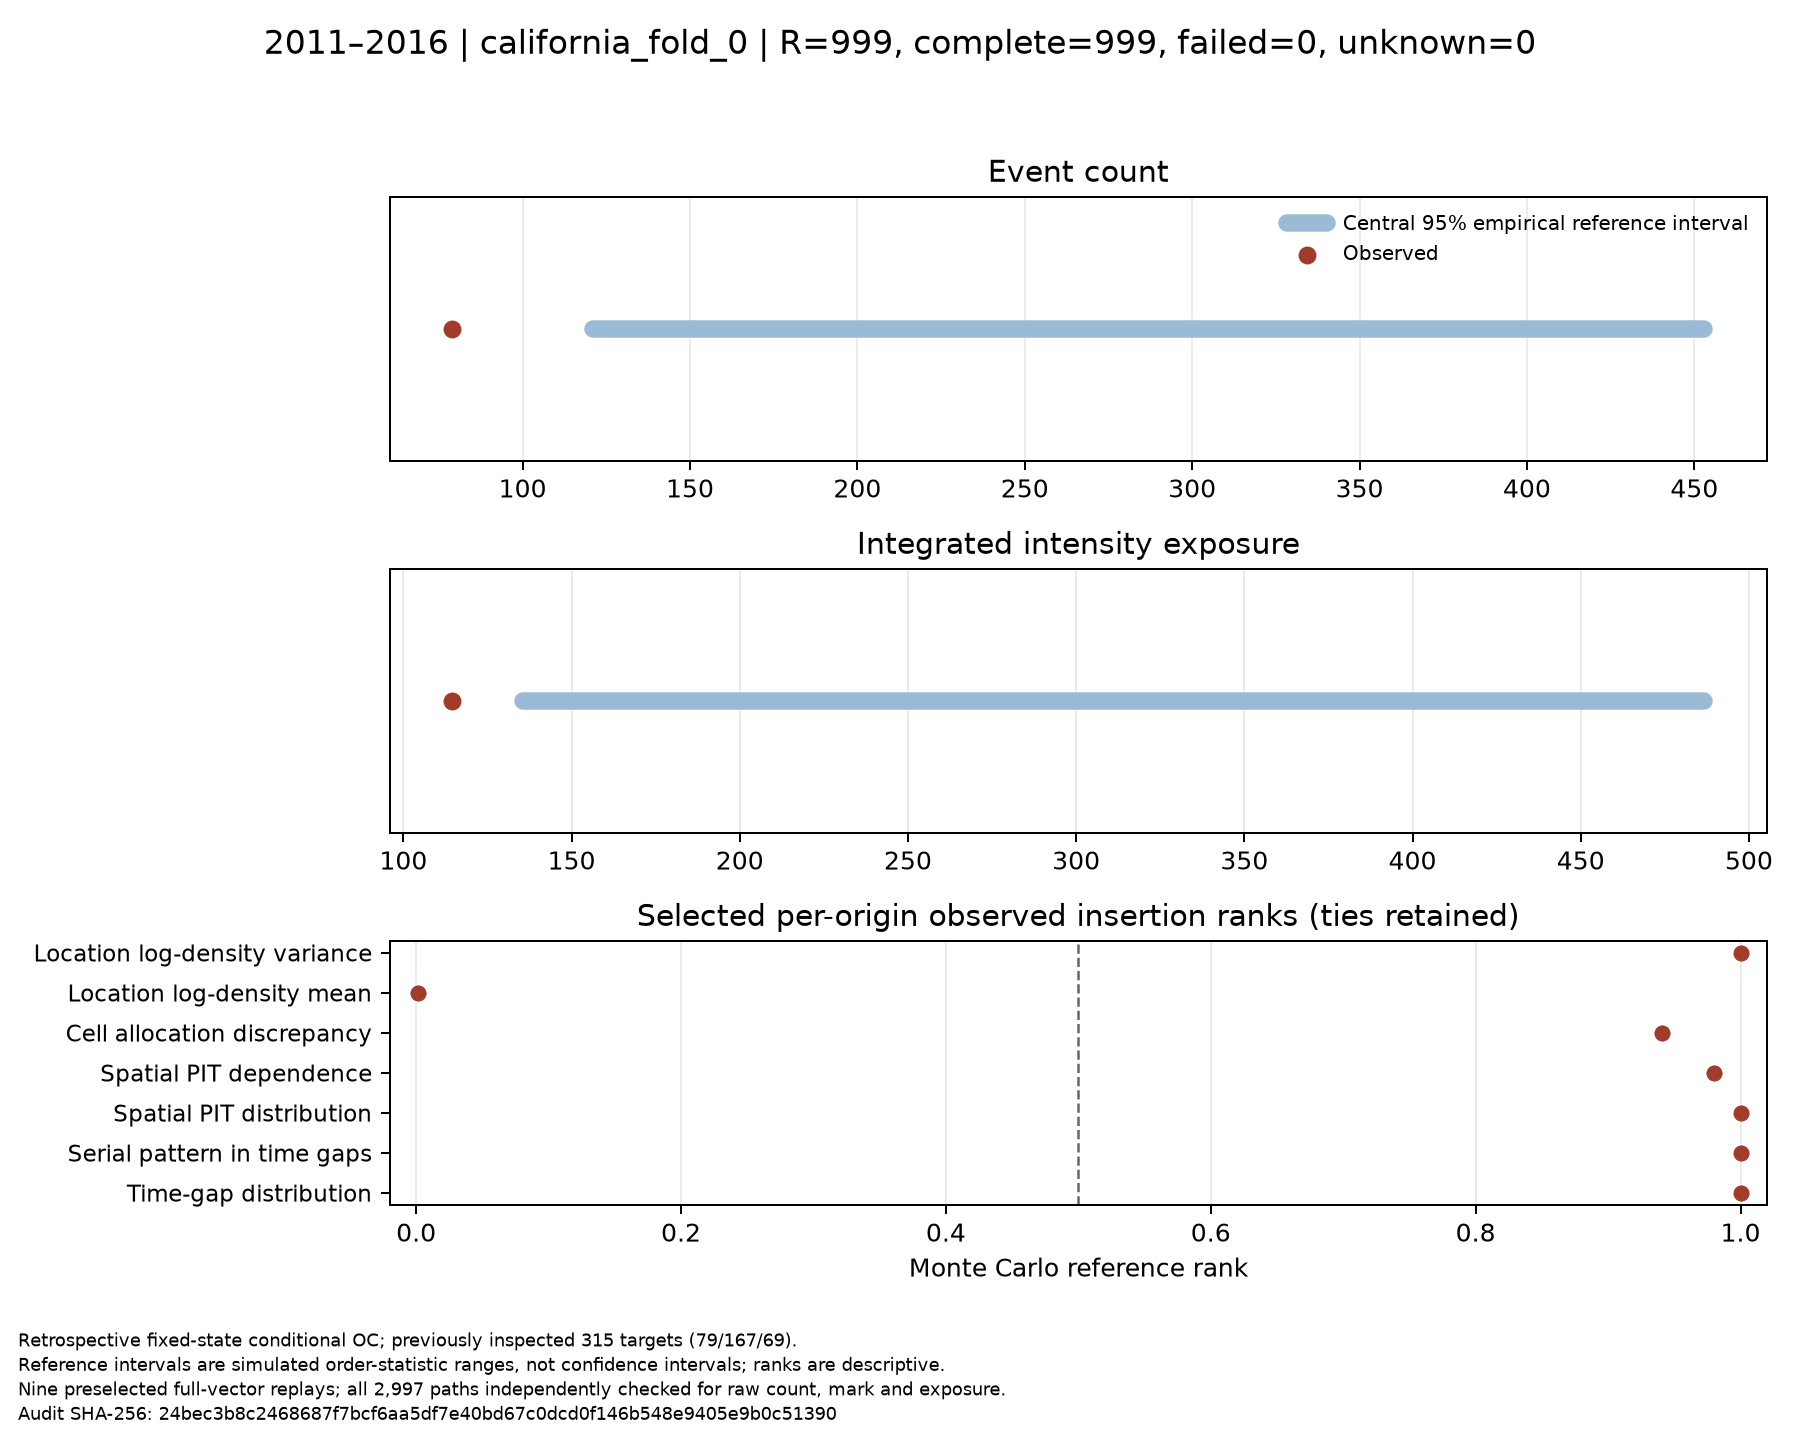
\includegraphics[width=\linewidth,height=.78\textheight,keepaspectratio]{spatial_detail_origin_01.png}
\caption{Conditional diagnostic insertion intervals for frozen OC Fold 0 (2011--2016; 79 observed targets). Immigrant exposure is deterministic; its ties carry no adequacy evidence. Other ties and ordinary-looking coordinates coexist with discrepancies. These are descriptive reference comparisons.}\end{figure}
\clearpage

\clearpage
\begin{figure}[p]\centering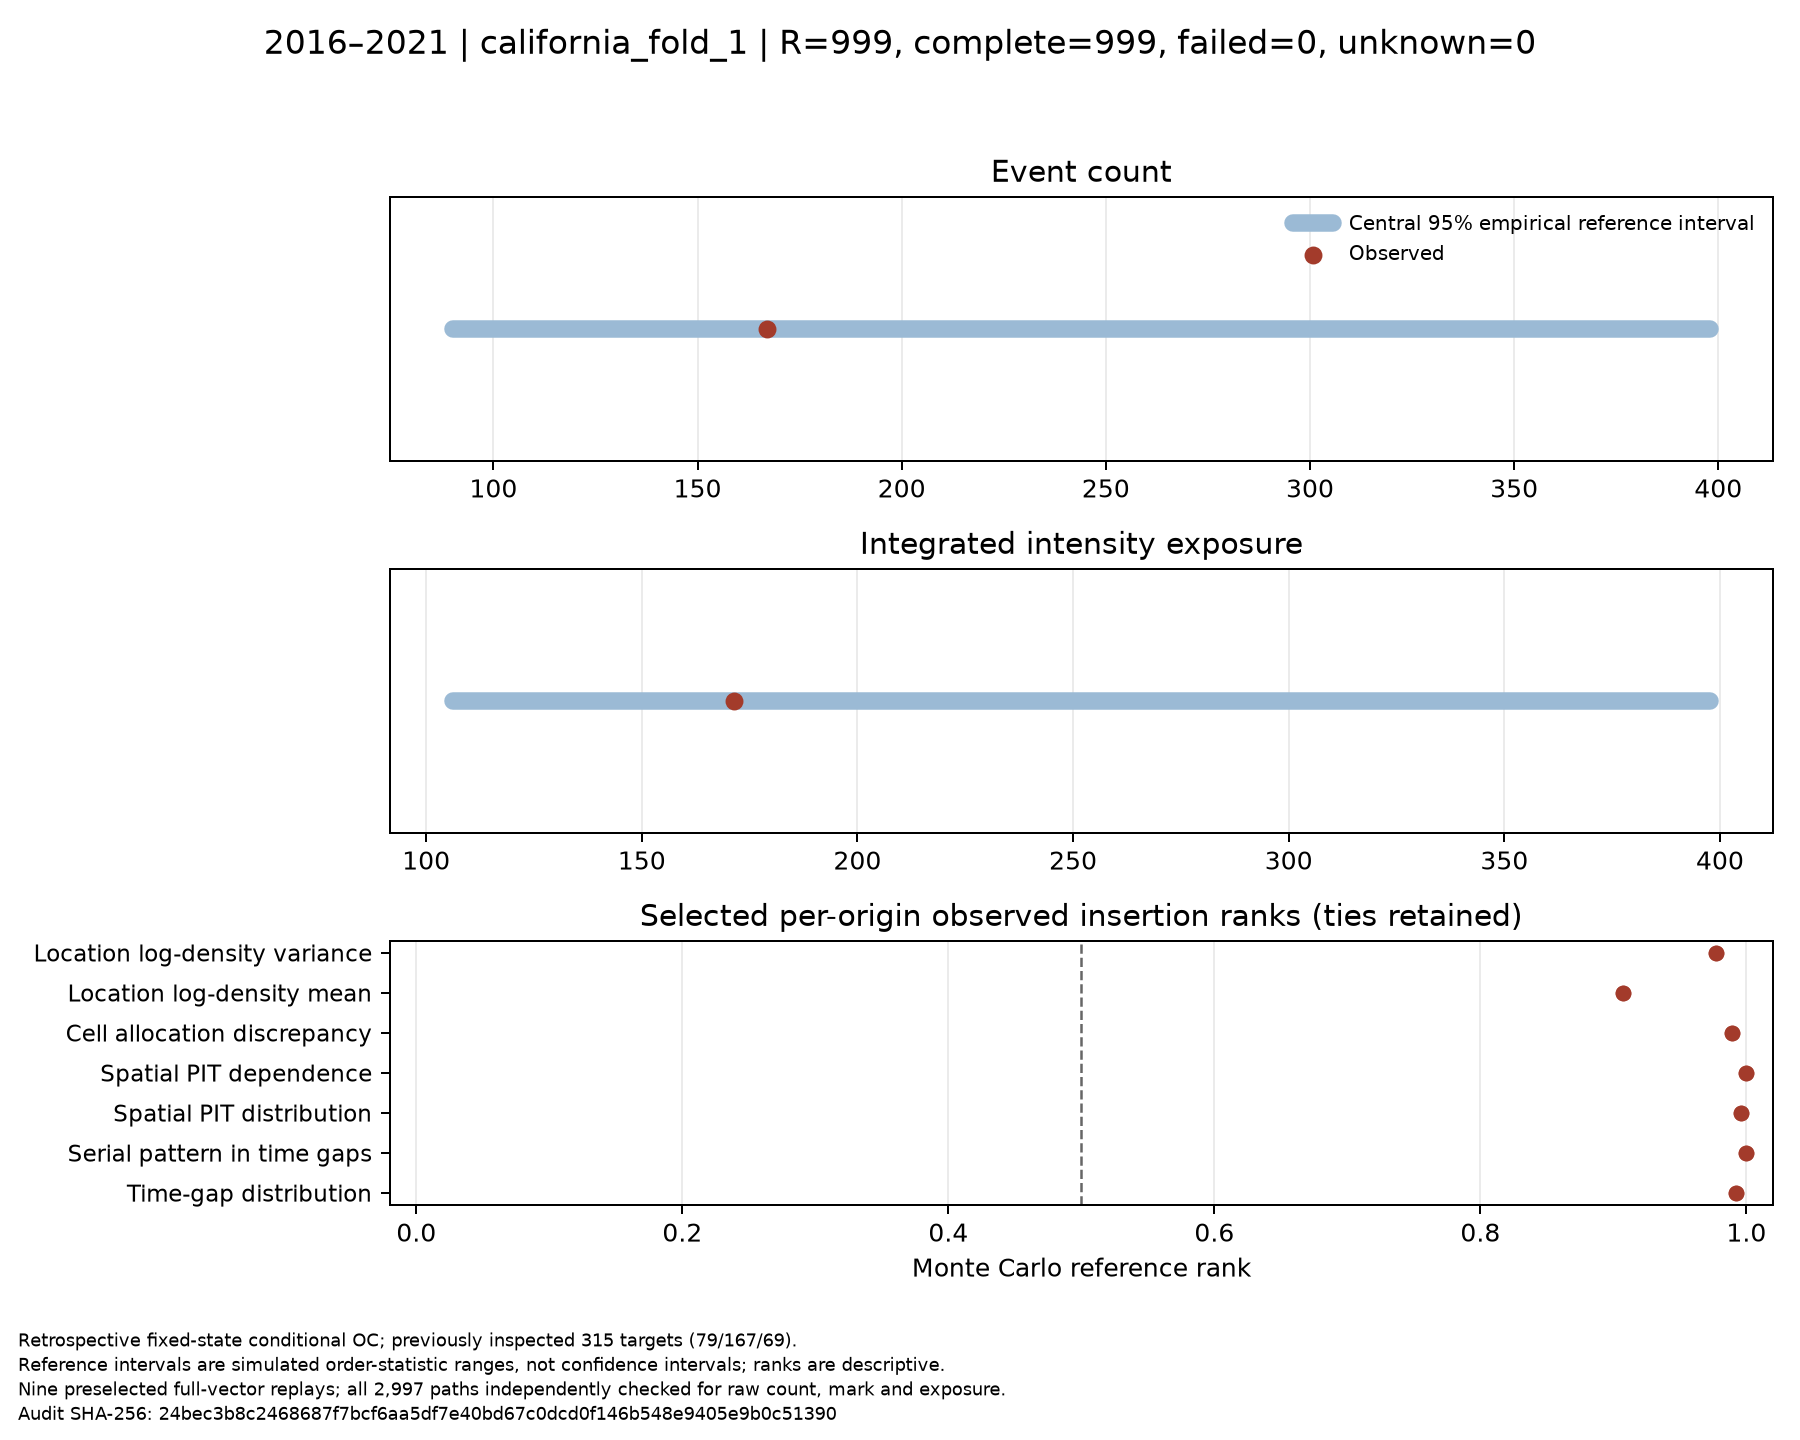
\includegraphics[width=\linewidth,height=.78\textheight,keepaspectratio]{spatial_detail_origin_02.png}
\caption{Conditional diagnostic insertion intervals for frozen OC Fold 1 (2016--2021; 167 observed targets). Immigrant exposure is deterministic; its ties carry no adequacy evidence. Other ties and ordinary-looking coordinates coexist with discrepancies. These are descriptive reference comparisons.}\end{figure}
\clearpage

\clearpage
\begin{figure}[p]\centering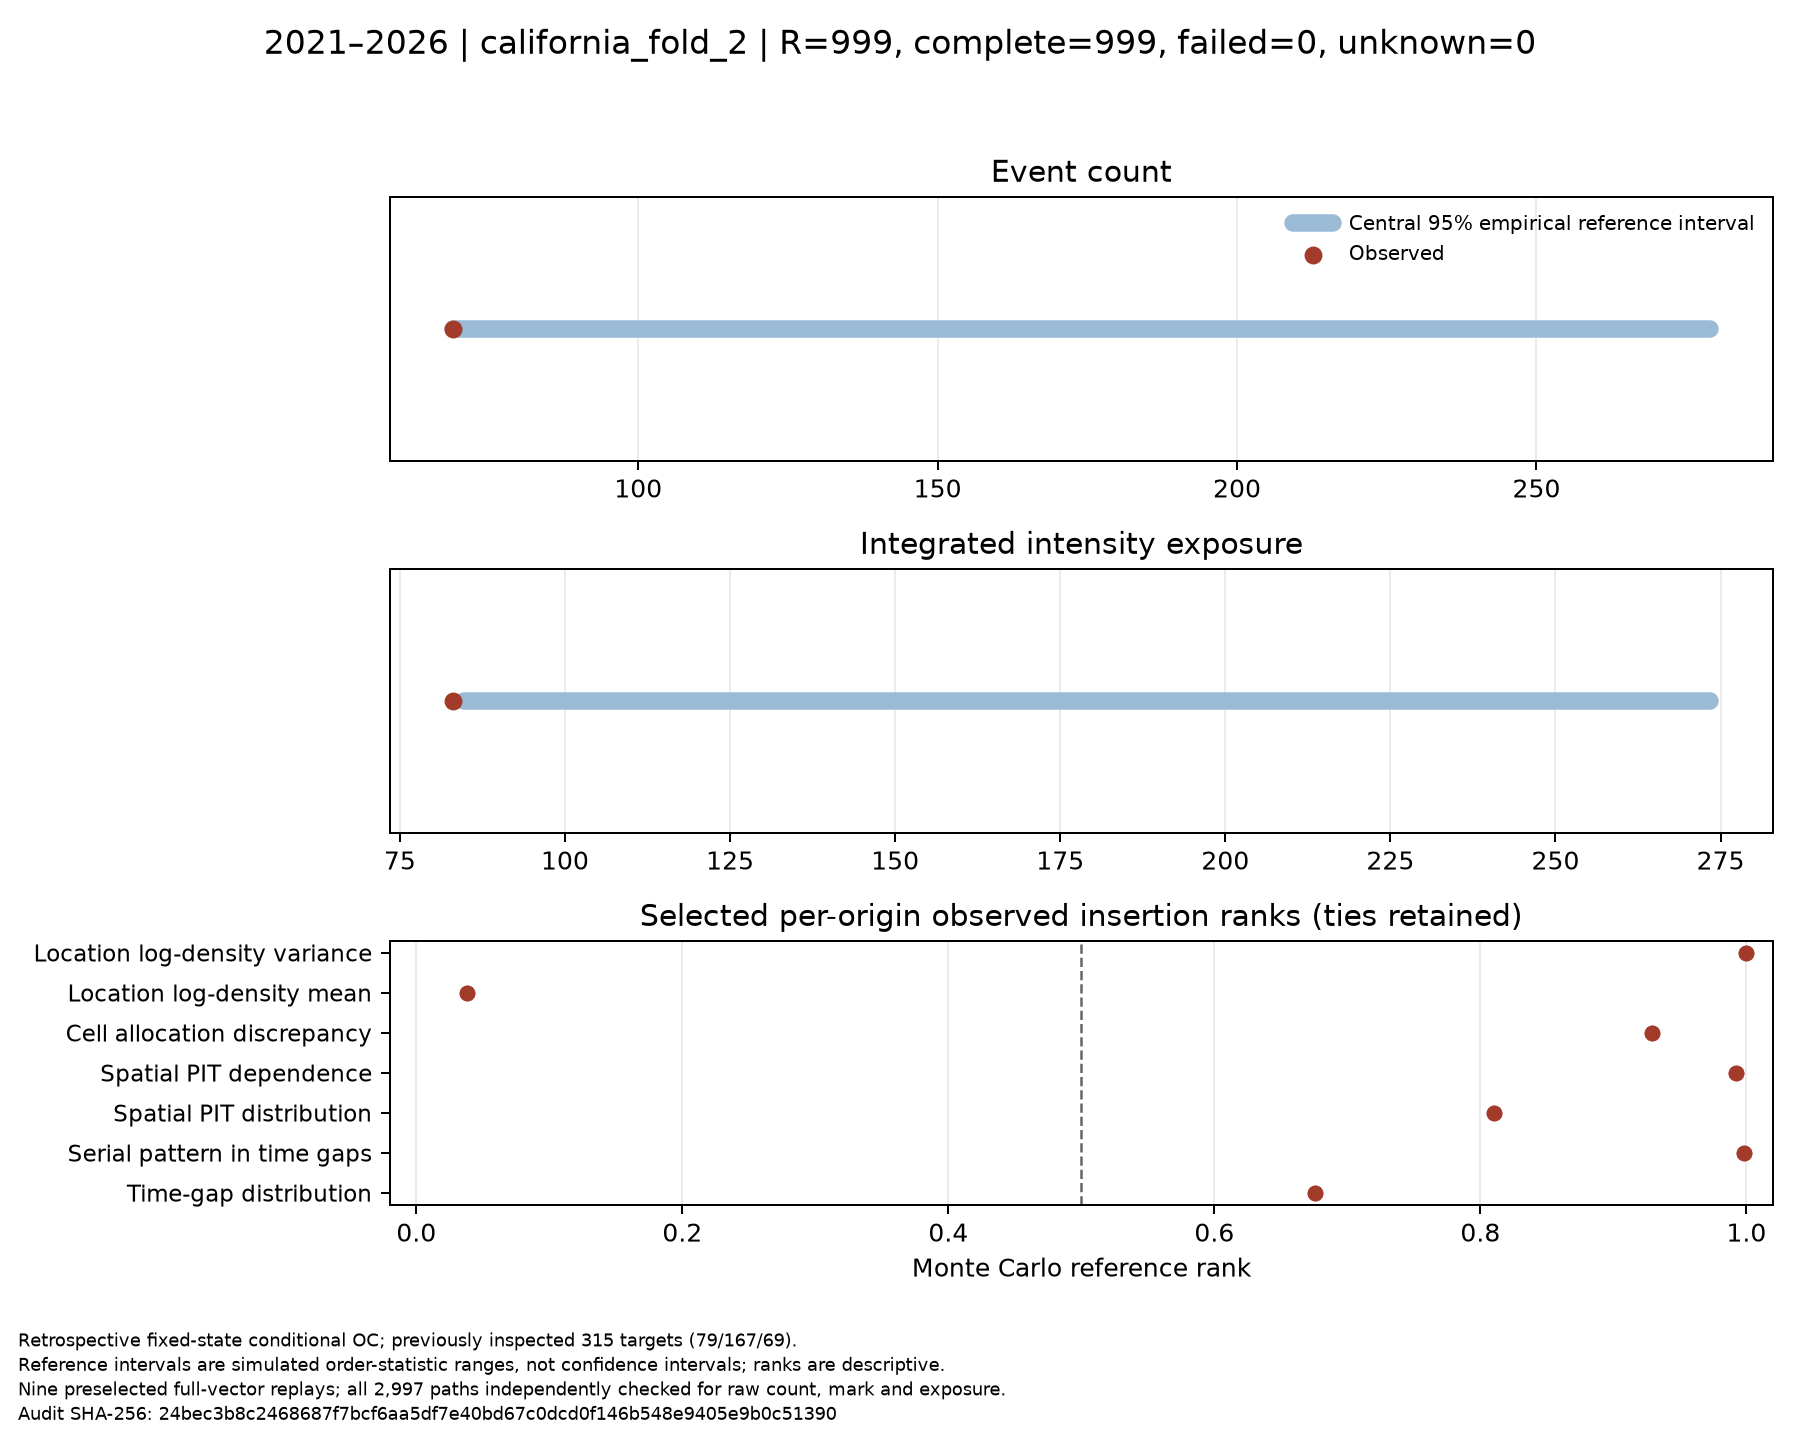
\includegraphics[width=\linewidth,height=.78\textheight,keepaspectratio]{spatial_detail_origin_03.png}
\caption{Conditional diagnostic insertion intervals for frozen OC Fold 2 (2021--2026; 69 observed targets). Immigrant exposure is deterministic; its ties carry no adequacy evidence. Other ties and ordinary-looking coordinates coexist with discrepancies. These are descriptive reference comparisons.}\end{figure}
\clearpage


{\small\setlength{\bibsep}{4pt}\bibliographystyle{plainnat}\bibliography{references}}
\end{document}
